%%%%%%%%%%%%%%%%%%%%%%%%%%%%%%%Packages%%%%%%%%%%%%%%%%%%%%%%%%%%%%%%%%
\documentclass[12pt,openright]{book}
\usepackage{iftex}
\iftutex
  % Moteurs Unicode (XeLaTeX/LuaLaTeX)
  \usepackage{fontspec}
  \usepackage{polyglossia}
  \setmainlanguage{french}
  % Définition d'une commande \nombre équivalente
\newcommand{\nombre}[1]{\numprint{#1}}
\else
  % Moteur classique (pdfLaTeX)
  \usepackage[T1]{fontenc}
  \usepackage[utf8]{inputenc}
  \usepackage[french]{babel}
\fi
\usepackage[a4paper,inner=1.2cm,outer=0.8cm,top=2cm,bottom=2cm]{geometry}
\usepackage{datatool}
\DTLsetseparator{;} % Avant tout : on a besoin de définir le séparateur pour la basededonnées
\usepackage{numprint}
\npthousandsep{\,} % espace fine insécable entre les milliers (usage français)
%\usepackage[noenc]{tipa}
%\usepackage{tipa}
\usepackage{tipx}
%\usepackage[geometry,weather,misc,clock]{ifsym}
\usepackage{pifont}
\usepackage{eurosym}
%\usepackage{amsmath}
\usepackage{wasysym}
%\usepackage{amssymb,amsfonts,textcomp}
%\usepackage[T3,T1]{fontenc}
\usepackage[dvipdfm]{graphicx} % Pour les images
\usepackage{metalogo}
\usepackage{xifthen} % Programmation dans LaTeX
\usepackage{multicol}
\usepackage{array}
\usepackage{multirow}
\usepackage{makecell}
\usepackage{tabularx}
\usepackage{colortbl}
\usepackage[most]{tcolorbox}
\usepackage{enumitem}
\usepackage{booktabs}
\usepackage[table,xcdraw]{xcolor}
\usepackage{caption}
\DeclareCaptionFormat{sanslabel}{#3}
\usepackage{xspace}
\usepackage{xstring}
\usepackage{xfp}%Gestion des pourcentages
\usepackage{tikz}
\usetikzlibrary{babel}
\usepackage{pgf-pie}
\usepackage{pgfplots}
\pgfplotsset{compat=1.18}
\usepackage{changepage}
\usepackage[defaultlines=2]{nowidow}
\usepackage{xpatch} % Nécessaire pour modifier l'alignement des ndbp/Manier avec précaution
\usepackage{xparse}
\usepackage{etoolbox} % Ajouts de commandes pour résoudre des problèmes d'espacement notamment
\usepackage{setspace} % Pour changer l'espacement entre les lignes
\usepackage{shorttoc}
\usepackage{titlesec}
\usepackage{titletoc}
\usepackage{tocbibind} % rajoute la bib, l'ind, la ToC, la lof et la lot automatiquement à ToC.
\usepackage{totpages} % Pour obtenir le numéro de la dernière page
\usepackage{perpage} % Permet de recommencer les ndbp à chaque page
\MakePerPage{footnote} % Appliquer le changement des ndbp
\usepackage{fancyhdr} % Pour maîtriser les en-têtes
\usepackage{xkeyval}
\usepackage{longtable}
\usepackage{microtype} %Résolution de certains problèmes de dépassement d'hbox
\usepackage{needspace}
\usepackage{morewrites}
\usepackage{pdflscape}
\usepackage{pdfpages} % Insérer des pdf dans le fichier
\usepackage[xindy]{imakeidx} % Pour l'index
\title{Banque indexée des sujets d'Humanités, Terminale}
\author{Mikaël Quesseveur}
\date{2025-09-22}

\renewcommand{\thesubsection}{\arabic{section}.\arabic{subsection}.}

\titleformat{\subsection}
{\normalfont\large\bfseries}{\thesubsection}{1em}{}

\titleformat{\subsubsection}
{\center\normalfont\normalsize\bfseries}{\thesubsubsection}{1em}{}

%\titleformat*{\subsubsection}{\center\bfseries}

%%%Configuration de dots pour qu'il soit plus élégant et supprimer l'espace inélégante dans le cas où les points de suspension sont entre crochets%%%
\let\olddots\dots
\renewcommand\dots{\olddots{}\xspace}
\xspaceaddexceptions{]}

%%%Reconfiguration des colonnes de tabularx pour améliorer l'espacement%%%
\renewcommand{\tabularxcolumn}[1]{>{\centering\arraybackslash}m{#1}}

%%%%%%%%%%%%%%%%%%%%%%%%%%%%%%%%%%%%%%%%%%%%%%%%%%%%%%%%%%%%%%%%%%%%%%
%%%%%%%%%%%%%%%%%%%%%Commandes pour l'index%%%%%%%%%%%%%%%%%%%%%%%%%%%
%%%%%%%%%%%%%%%%%%%%%%%%%%%%%%%%%%%%%%%%%%%%%%%%%%%%%%%%%%%%%%%%%%%%%%
\newcommand{\questiontitle}{\bfseries\large}
\newcommand{\questiontype}{\itshape\normalsize}
\newcommand{\questionsize}[1]{{\normalfont\footnotesize#1}}
%%%Changement de l'indentation dans les index%%%
\makeatletter
\def\@idxitem{\par\hangindent 12pt}
\makeatother

%%%Gestion de l'espacement dans les environnements d'index
\AtBeginEnvironment{theindex}{\raggedbottom}  % nécessite etoolbox

%%%Les liens vers les banques de sujets%%%

\newcommand{\sujetshlpsanscorr}{\href{https://drive.google.com/file/d/127SoEaNlMn662R3lhdlSIw74tFSGJGNQ/view?usp=drive_link}{Banque de sujets HLP sans éléments d'évaluation}}
\newcommand{\sujetshlpcorr}{\href{https://drive.google.com/file/d/1PJyaKCNypSU1-v5-fRtyrf5YMxSI8puw/view?usp=drive_link}{Banque de sujets HLP avec éléments d'évaluation}}
\newcommand{\sujetscsv}{\href{https://docs.google.com/spreadsheets/d/1cosKjvc7rgAi1zdjNtZ4UWY1j2-Tbmz-K3ha3xRiIc4/edit?usp=sharing}{Tableau (\textit{Sheets, en ligne)} récapitulant les sujets et leur indexation}}

%%%%%%%%%%%%%%%%%%%%%%%%%%%%%%%%%%%%%%%%%%%%%%%%%%%%%%%%%%%%%%%%%%%%%%%
%%%%%%%%%%%%%%%%%%%%%%%%% Compteurs %%%%%%%%%%%%%%%%%%%%%%%%%%%%%%%%%%%
%%%%%%%%%%%%%%%%%%%%%%%%%%%%%%%%%%%%%%%%%%%%%%%%%%%%%%%%%%%%%%%%%%%%%%%
%%%%%%%%%%%%%%%%%%%%%%%%%%%%%%%%%%%%%%%%%%%%%%%%%%%%%%%%%%%%%%%%%%%%%%%
%%%%%%%%%%%%%%%%%%%%%%%%%%%%%%Compteurs%%%%%%%%%%%%%%%%%%%%%%%%%%%%%%%%
%%%%%%%%%%%%%%%%%%%%%%%%%%%%%%%%%%%%%%%%%%%%%%%%%%%%%%%%%%%%%%%%%%%%%%%
%%%Compter les sujets par thème%%%
\newcounter{nosujet}
\newcounter{sujetHQ}
\newcounter{sujetRS}
%%%Sujets simples%%%
\newcounter{sujetEXS}
\newcounter{sujetETA}
\newcounter{sujetMM}
\newcounter{sujetHV}
\newcounter{sujetCC}
\newcounter{sujetHL}
%%%Sujets mixtes%%%
\newcounter{sujetEXSTA}
\newcounter{sujetEXSMM}
\newcounter{sujetETAMM}
\newcounter{sujetOdS}
\newcounter{sujetHVL}
\newcounter{sujetHVCC}
\newcounter{sujetHLCC}
\newcounter{sujetOdH}
%%%Sujets mixtes semestres%%%
\newcounter{sujetETACC}
\newcounter{sujetETAHV}
\newcounter{sujetETAHL}
\newcounter{sujetEXSCC}
\newcounter{sujetEXSHV}
\newcounter{sujetEXSHL}
\newcounter{sujetMMCC}
\newcounter{sujetMMHV}
\newcounter{sujetMMHL}

%%%Sujets mixtes années%%
\newcounter{sujetpremterm}%%%Compteur général de sujet
\newcounter{sujetETAPdP}
\newcounter{sujetETADFI}
\newcounter{sujetETADMRC}
\newcounter{sujetETAHA}
\newcounter{sujetpremtermETA}
\newcounter{sujetEXSPdP}
\newcounter{sujetEXSDFI}
\newcounter{sujetEXSDMRC}
\newcounter{sujetEXSHA}
\newcounter{sujetpremtermEXS}
\newcounter{sujetMMPdP}
\newcounter{sujetMMDFI}
\newcounter{sujetMMDMRC}
\newcounter{sujetMMHA}
\newcounter{sujetpremtermMM}
\newcounter{sujetCCPdP}
\newcounter{sujetCCDFI}
\newcounter{sujetCCDMRC}
\newcounter{sujetCCHA}
\newcounter{sujetpremtermCC}
\newcounter{sujetHVPdP}
\newcounter{sujetHVDFI}
\newcounter{sujetHVDMRC}
\newcounter{sujetHVHA}
\newcounter{sujetpremtermHV}
\newcounter{sujetHLPdP}
\newcounter{sujetHLDFI}
\newcounter{sujetHLDMRC}
\newcounter{sujetHLHA}
\newcounter{sujetpremtermHL}
\newcounter{sujetRSPdP}
\newcounter{sujetRSRdM}
\newcounter{sujetRSDFI}
\newcounter{sujetRSDMRC}
\newcounter{sujetRSHA}
\newcounter{sujetHQPdP}
\newcounter{sujetHQRdM}
\newcounter{sujetHQDFI}
\newcounter{sujetHQDMRC}
\newcounter{sujetHQHA}

%%%Somme des compteurs%%%
\newcounter{sujetall}
\newcounter{sujetallETA}
\newcounter{sujetallEXS}
\newcounter{sujetallMM}
\newcounter{sujetallRS}
\newcounter{sujetallCC}
\newcounter{sujetallHV}
\newcounter{sujetallHL}
\newcounter{sujetallHQ}

%%%Compter les sujets par thème et types de questions%%%
%%%%%%%%%%%%%%%%%%%%%%%%%%%%%%%%%%%%%%%%%%%%%
%%%%%%%%%Question d'interprétation%%%%%%%%%%%
%%%%%%%%%%%%%%%%%%%%%%%%%%%%%%%%%%%%%%%%%%%%%

%%%%%%%%%%%%%%%Général%%%%%%%%%%%%%%%%%%%%%%%
\newcounter{nosujetint}
\newcounter{sujetHQint}
\newcounter{sujetRSint}
%%%Sujets simples%%%
\newcounter{sujetintEXS}
\newcounter{sujetintETA}
\newcounter{sujetintMM}
\newcounter{sujetintHV}
\newcounter{sujetintCC}
\newcounter{sujetintHL}
%%%Sujets mixtes%%%
\newcounter{sujetintEXSTA}
\newcounter{sujetintEXSMM}
\newcounter{sujetintETAMM}
\newcounter{sujetintOdS}
\newcounter{sujetintHVL}
\newcounter{sujetintHVCC}
\newcounter{sujetintHLCC}
\newcounter{sujetintOdH}
%%%Sujets mixtes semestres%%%
\newcounter{sujetintETACC}
\newcounter{sujetintETAHV}
\newcounter{sujetintETAHL}
\newcounter{sujetintEXSCC}
\newcounter{sujetintEXSHV}
\newcounter{sujetintEXSHL}
\newcounter{sujetintMMCC}
\newcounter{sujetintMMHV}
\newcounter{sujetintMMHL}
%%%Sujets mixtes années%%
\newcounter{sujetintpremterm}
\newcounter{sujetintpremtermRS}
\newcounter{sujetintpremtermHQ}
\newcounter{sujetintETAPdP}
\newcounter{sujetintETADFI}
\newcounter{sujetintETADMRC}
\newcounter{sujetintETAHA}
\newcounter{sujetintpremtermETA}
\newcounter{sujetintEXSPdP}
\newcounter{sujetintEXSDFI}
\newcounter{sujetintEXSDMRC}
\newcounter{sujetintEXSHA}
\newcounter{sujetintpremtermEXS}
\newcounter{sujetintMMPdP}
\newcounter{sujetintMMDFI}
\newcounter{sujetintMMDMRC}
\newcounter{sujetintMMHA}
\newcounter{sujetintpremtermMM}
\newcounter{sujetintCCPdP}
\newcounter{sujetintCCDFI}
\newcounter{sujetintCCDMRC}
\newcounter{sujetintCCHA}
\newcounter{sujetintpremtermCC}
\newcounter{sujetintHVPdP}
\newcounter{sujetintHVDFI}
\newcounter{sujetintHVDMRC}
\newcounter{sujetintHVHA}
\newcounter{sujetintpremtermHV}
\newcounter{sujetintHLPdP}
\newcounter{sujetintHLDFI}
\newcounter{sujetintHLDMRC}
\newcounter{sujetintHLHA}
\newcounter{sujetintpremtermHL}
\newcounter{sujetintRSPdP}
\newcounter{sujetintRSRdM}
\newcounter{sujetintRSDFI}
\newcounter{sujetintRSDMRC}
\newcounter{sujetintRSHA}
\newcounter{sujetintHQPdP}
\newcounter{sujetintHQRdM}
\newcounter{sujetintHQDFI}
\newcounter{sujetintHQDMRC}
\newcounter{sujetintHQHA}
%%%Somme des compteurs%%%
\newcounter{sujetallintETA}
\newcounter{sujetallintEXS}
\newcounter{sujetallintMM}
\newcounter{sujetallintRS}
\newcounter{sujetallintCC}
\newcounter{sujetallintHV}
\newcounter{sujetallintHL}
\newcounter{sujetallintHQ}

%%%%%%%%Interprétation philosophique%%%%%%%%%
\newcounter{nosujetintphilosophique}
\newcounter{sujetHQintphilosophique}
\newcounter{sujetRSintphilosophique}
%%%Sujets simples%%%
\newcounter{sujetintphilosophiqueEXS}
\newcounter{sujetintphilosophiqueETA}
\newcounter{sujetintphilosophiqueMM}
\newcounter{sujetintphilosophiqueHV}
\newcounter{sujetintphilosophiqueCC}
\newcounter{sujetintphilosophiqueHL}
%%%Sujets mixtes%%%
\newcounter{sujetintphilosophiqueEXSTA}
\newcounter{sujetintphilosophiqueEXSMM}
\newcounter{sujetintphilosophiqueETAMM}
\newcounter{sujetintphilosophiqueOdS}
\newcounter{sujetintphilosophiqueHVL}
\newcounter{sujetintphilosophiqueHVCC}
\newcounter{sujetintphilosophiqueHLCC}
\newcounter{sujetintphilosophiqueOdH}
%%%Sujets mixtes semestres%%%
\newcounter{sujetintphilosophiqueETACC}
\newcounter{sujetintphilosophiqueETAHV}
\newcounter{sujetintphilosophiqueETAHL}
\newcounter{sujetintphilosophiqueEXSCC}
\newcounter{sujetintphilosophiqueEXSHV}
\newcounter{sujetintphilosophiqueEXSHL}
\newcounter{sujetintphilosophiqueMMCC}
\newcounter{sujetintphilosophiqueMMHV}
\newcounter{sujetintphilosophiqueMMHL}
%%%Sujets mixtes années%%
\newcounter{sujetintphilosophiquepremterm}
\newcounter{sujetintphilosophiquepremtermRS}
\newcounter{sujetintphilosophiquepremtermHQ}
\newcounter{sujetintphilosophiqueETAPdP}
\newcounter{sujetintphilosophiqueETADFI}
\newcounter{sujetintphilosophiqueETADMRC}
\newcounter{sujetintphilosophiqueETAHA}
\newcounter{sujetintphilosophiquepremtermETA}
\newcounter{sujetintphilosophiqueEXSPdP}
\newcounter{sujetintphilosophiqueEXSDFI}
\newcounter{sujetintphilosophiqueEXSDMRC}
\newcounter{sujetintphilosophiqueEXSHA}
\newcounter{sujetintphilosophiquepremtermEXS}
\newcounter{sujetintphilosophiqueMMPdP}
\newcounter{sujetintphilosophiqueMMDFI}
\newcounter{sujetintphilosophiqueMMDMRC}
\newcounter{sujetintphilosophiqueMMHA}
\newcounter{sujetintphilosophiquepremtermMM}
\newcounter{sujetintphilosophiqueCCPdP}
\newcounter{sujetintphilosophiqueCCDFI}
\newcounter{sujetintphilosophiqueCCDMRC}
\newcounter{sujetintphilosophiqueCCHA}
\newcounter{sujetintphilosophiquepremtermCC}
\newcounter{sujetintphilosophiqueHVPdP}
\newcounter{sujetintphilosophiqueHVDFI}
\newcounter{sujetintphilosophiqueHVDMRC}
\newcounter{sujetintphilosophiqueHVHA}
\newcounter{sujetintphilosophiquepremtermHV}
\newcounter{sujetintphilosophiqueHLPdP}
\newcounter{sujetintphilosophiqueHLDFI}
\newcounter{sujetintphilosophiqueHLDMRC}
\newcounter{sujetintphilosophiqueHLHA}
\newcounter{sujetintphilosophiquepremtermHL}
\newcounter{sujetintphilosophiqueRSPdP}
\newcounter{sujetintphilosophiqueRSRdM}
\newcounter{sujetintphilosophiqueRSDFI}
\newcounter{sujetintphilosophiqueRSDMRC}
\newcounter{sujetintphilosophiqueRSHA}
\newcounter{sujetintphilosophiqueHQPdP}
\newcounter{sujetintphilosophiqueHQRdM}
\newcounter{sujetintphilosophiqueHQDFI}
\newcounter{sujetintphilosophiqueHQDMRC}
\newcounter{sujetintphilosophiqueHQHA}
%%%Somme des compteurs%%%
\newcounter{sujetallintphilosophiqueETA}
\newcounter{sujetallintphilosophiqueEXS}
\newcounter{sujetallintphilosophiqueMM}
\newcounter{sujetallintphilosophiqueRS}
\newcounter{sujetallintphilosophiqueCC}
\newcounter{sujetallintphilosophiqueHV}
\newcounter{sujetallintphilosophiqueHL}
\newcounter{sujetallintphilosophiqueHQ}

%%%%%%%%%Interprétation littéraire%%%%%%%%%%%
\newcounter{nosujetintlitteraire}
\newcounter{sujetHQintlitteraire}
\newcounter{sujetRSintlitteraire}
%%%Sujets simples%%%
\newcounter{sujetintlitteraireEXS}
\newcounter{sujetintlitteraireETA}
\newcounter{sujetintlitteraireMM}
\newcounter{sujetintlitteraireHV}
\newcounter{sujetintlitteraireCC}
\newcounter{sujetintlitteraireHL}
%%%Sujets mixtes%%%
\newcounter{sujetintlitteraireEXSTA}
\newcounter{sujetintlitteraireEXSMM}
\newcounter{sujetintlitteraireETAMM}
\newcounter{sujetintlitteraireOdS}
\newcounter{sujetintlitteraireHVL}
\newcounter{sujetintlitteraireHVCC}
\newcounter{sujetintlitteraireHLCC}
\newcounter{sujetintlitteraireOdH}
%%%Sujets mixtes semestres%%%
\newcounter{sujetintlitteraireETACC}
\newcounter{sujetintlitteraireETAHV}
\newcounter{sujetintlitteraireETAHL}
\newcounter{sujetintlitteraireEXSCC}
\newcounter{sujetintlitteraireEXSHV}
\newcounter{sujetintlitteraireEXSHL}
\newcounter{sujetintlitteraireMMCC}
\newcounter{sujetintlitteraireMMHV}
\newcounter{sujetintlitteraireMMHL}
%%%Sujets mixtes années%%
\newcounter{sujetintlitterairepremterm}
\newcounter{sujetintlitterairepremtermRS}
\newcounter{sujetintlitterairepremtermHQ}
\newcounter{sujetintlitteraireETAPdP}
\newcounter{sujetintlitteraireETADFI}
\newcounter{sujetintlitteraireETADMRC}
\newcounter{sujetintlitteraireETAHA}
\newcounter{sujetintlitterairepremtermETA}
\newcounter{sujetintlitteraireEXSPdP}
\newcounter{sujetintlitteraireEXSDFI}
\newcounter{sujetintlitteraireEXSDMRC}
\newcounter{sujetintlitteraireEXSHA}
\newcounter{sujetintlitterairepremtermEXS}
\newcounter{sujetintlitteraireMMPdP}
\newcounter{sujetintlitteraireMMDFI}
\newcounter{sujetintlitteraireMMDMRC}
\newcounter{sujetintlitteraireMMHA}
\newcounter{sujetintlitterairepremtermMM}
\newcounter{sujetintlitteraireCCPdP}
\newcounter{sujetintlitteraireCCDFI}
\newcounter{sujetintlitteraireCCDMRC}
\newcounter{sujetintlitteraireCCHA}
\newcounter{sujetintlitterairepremtermCC}
\newcounter{sujetintlitteraireHVPdP}
\newcounter{sujetintlitteraireHVDFI}
\newcounter{sujetintlitteraireHVDMRC}
\newcounter{sujetintlitteraireHVHA}
\newcounter{sujetintlitterairepremtermHV}
\newcounter{sujetintlitteraireHLPdP}
\newcounter{sujetintlitteraireHLDFI}
\newcounter{sujetintlitteraireHLDMRC}
\newcounter{sujetintlitteraireHLHA}
\newcounter{sujetintlitterairepremtermHL}
\newcounter{sujetintlitteraireRSPdP}
\newcounter{sujetintlitteraireRSRdM}
\newcounter{sujetintlitteraireRSDFI}
\newcounter{sujetintlitteraireRSDMRC}
\newcounter{sujetintlitteraireRSHA}
\newcounter{sujetintlitteraireHQPdP}
\newcounter{sujetintlitteraireHQRdM}
\newcounter{sujetintlitteraireHQDFI}
\newcounter{sujetintlitteraireHQDMRC}
\newcounter{sujetintlitteraireHQHA}
%%%Somme des compteurs%%%
\newcounter{sujetallintlitteraireETA}
\newcounter{sujetallintlitteraireEXS}
\newcounter{sujetallintlitteraireMM}
\newcounter{sujetallintlitteraireRS}
\newcounter{sujetallintlitteraireCC}
\newcounter{sujetallintlitteraireHV}
\newcounter{sujetallintlitteraireHL}
\newcounter{sujetallintlitteraireHQ}

%%%%%%%%%%%%%%%%%%%%%%%%%%%%%%%%%%%%%%%%%%%%%
%%%%%%%%%%%%Question de réflexion%%%%%%%%%%%%
%%%%%%%%%%%%%%%%%%%%%%%%%%%%%%%%%%%%%%%%%%%%%
\newcounter{nosujetref}
%%%Sujets simples%%%
\newcounter{sujetrefEXS}
\newcounter{sujetrefETA}
\newcounter{sujetrefMM}
\newcounter{sujetrefHV}
\newcounter{sujetrefCC}
\newcounter{sujetrefHL}
%%%Sujets mixtes%%%
\newcounter{sujetrefEXSTA}
\newcounter{sujetrefEXSMM}
\newcounter{sujetrefETAMM}
\newcounter{sujetrefOdS}
\newcounter{sujetrefHVL}
\newcounter{sujetrefHVCC}
\newcounter{sujetrefHLCC}
\newcounter{sujetrefOdH}
%%%Sujets mixtes semestres%%%
\newcounter{sujetrefETACC}
\newcounter{sujetrefETAHV}
\newcounter{sujetrefETAHL}
\newcounter{sujetrefEXSCC}
\newcounter{sujetrefEXSHV}
\newcounter{sujetrefEXSHL}
\newcounter{sujetrefMMCC}
\newcounter{sujetrefMMHV}
\newcounter{sujetrefMMHL}
%%%Sujets mixtes années%%
\newcounter{sujetrefpremterm}%%%Compteur général
\newcounter{sujetrefETAPdP}
\newcounter{sujetrefETADFI}
\newcounter{sujetrefETADMRC}
\newcounter{sujetrefETAHA}
\newcounter{sujetrefpremtermETA}
\newcounter{sujetrefEXSPdP}
\newcounter{sujetrefEXSDFI}
\newcounter{sujetrefEXSDMRC}
\newcounter{sujetrefEXSHA}
\newcounter{sujetrefpremtermEXS}
\newcounter{sujetrefMMPdP}
\newcounter{sujetrefMMDFI}
\newcounter{sujetrefMMDMRC}
\newcounter{sujetrefMMHA}
\newcounter{sujetrefpremtermMM}
\newcounter{sujetrefCCPdP}
\newcounter{sujetrefCCDFI}
\newcounter{sujetrefCCDMRC}
\newcounter{sujetrefCCHA}
\newcounter{sujetrefpremtermCC}
\newcounter{sujetrefHVPdP}
\newcounter{sujetrefHVDFI}
\newcounter{sujetrefHVDMRC}
\newcounter{sujetrefHVHA}
\newcounter{sujetrefpremtermHV}
\newcounter{sujetrefHLPdP}
\newcounter{sujetrefHLDFI}
\newcounter{sujetrefHLDMRC}
\newcounter{sujetrefHLHA}
\newcounter{sujetrefpremtermHL}
\newcounter{sujetrefRSPdP}
\newcounter{sujetrefRSRdM}
\newcounter{sujetrefRSDFI}
\newcounter{sujetrefRSDMRC}
\newcounter{sujetrefRSHA}
\newcounter{sujetrefHQPdP}
\newcounter{sujetrefHQRdM}
\newcounter{sujetrefHQDFI}
\newcounter{sujetrefHQDMRC}
\newcounter{sujetrefHQHA}
%%%Somme des compteurs%%%
\newcounter{sujetallrefETA}
\newcounter{sujetallrefEXS}
\newcounter{sujetallrefMM}
\newcounter{sujetallrefRS}
\newcounter{sujetallrefCC}
\newcounter{sujetallrefHV}
\newcounter{sujetallrefHL}
\newcounter{sujetallrefHQ}

%%%%%%%%Réflexion philosophique%%%%%%%%%
\newcounter{nosujetrefphilosophique}
\newcounter{sujetHQrefphilosophique}
\newcounter{sujetRSrefphilosophique}
%%%Sujets simples%%%
\newcounter{sujetrefphilosophiqueEXS}
\newcounter{sujetrefphilosophiqueETA}
\newcounter{sujetrefphilosophiqueMM}
\newcounter{sujetrefphilosophiqueHV}
\newcounter{sujetrefphilosophiqueCC}
\newcounter{sujetrefphilosophiqueHL}
%%%Sujets mixtes%%%
\newcounter{sujetrefphilosophiqueEXSTA}
\newcounter{sujetrefphilosophiqueEXSMM}
\newcounter{sujetrefphilosophiqueETAMM}
\newcounter{sujetrefphilosophiqueOdS}
\newcounter{sujetrefphilosophiqueHVL}
\newcounter{sujetrefphilosophiqueHVCC}
\newcounter{sujetrefphilosophiqueHLCC}
\newcounter{sujetrefphilosophiqueOdH}
%%%Sujets mixtes semestres%%%
\newcounter{sujetrefphilosophiqueETACC}
\newcounter{sujetrefphilosophiqueETAHV}
\newcounter{sujetrefphilosophiqueETAHL}
\newcounter{sujetrefphilosophiqueEXSCC}
\newcounter{sujetrefphilosophiqueEXSHV}
\newcounter{sujetrefphilosophiqueEXSHL}
\newcounter{sujetrefphilosophiqueMMCC}
\newcounter{sujetrefphilosophiqueMMHV}
\newcounter{sujetrefphilosophiqueMMHL}
%%%Sujets mixtes années%%
\newcounter{sujetrefphilosophiquepremterm}
\newcounter{sujetrefphilosophiquepremtermRS}
\newcounter{sujetrefphilosophiquepremtermHQ}
\newcounter{sujetrefphilosophiqueETAPdP}
\newcounter{sujetrefphilosophiqueETADFI}
\newcounter{sujetrefphilosophiqueETADMRC}
\newcounter{sujetrefphilosophiqueETAHA}\newcounter{sujetrefphilosophiquepremtermETA}
\newcounter{sujetrefphilosophiqueEXSPdP}
\newcounter{sujetrefphilosophiqueEXSDFI}
\newcounter{sujetrefphilosophiqueEXSDMRC}
\newcounter{sujetrefphilosophiqueEXSHA}
\newcounter{sujetrefphilosophiquepremtermEXS}
\newcounter{sujetrefphilosophiqueMMPdP}
\newcounter{sujetrefphilosophiqueMMDFI}
\newcounter{sujetrefphilosophiqueMMDMRC}
\newcounter{sujetrefphilosophiqueMMHA}
\newcounter{sujetrefphilosophiquepremtermMM}
\newcounter{sujetrefphilosophiqueCCPdP}
\newcounter{sujetrefphilosophiqueCCDFI}
\newcounter{sujetrefphilosophiqueCCDMRC}
\newcounter{sujetrefphilosophiqueCCHA}
\newcounter{sujetrefphilosophiquepremtermCC}
\newcounter{sujetrefphilosophiqueHVPdP}
\newcounter{sujetrefphilosophiqueHVDFI}
\newcounter{sujetrefphilosophiqueHVDMRC}
\newcounter{sujetrefphilosophiqueHVHA}
\newcounter{sujetrefphilosophiquepremtermHV}
\newcounter{sujetrefphilosophiqueHLPdP}
\newcounter{sujetrefphilosophiqueHLDFI}
\newcounter{sujetrefphilosophiqueHLDMRC}
\newcounter{sujetrefphilosophiqueHLHA}
\newcounter{sujetrefphilosophiquepremtermHL}
\newcounter{sujetrefphilosophiqueRSPdP}
\newcounter{sujetrefphilosophiqueRSRdM}
\newcounter{sujetrefphilosophiqueRSDFI}
\newcounter{sujetrefphilosophiqueRSDMRC}
\newcounter{sujetrefphilosophiqueRSHA}
\newcounter{sujetrefphilosophiqueHQPdP}
\newcounter{sujetrefphilosophiqueHQRdM}
\newcounter{sujetrefphilosophiqueHQDFI}
\newcounter{sujetrefphilosophiqueHQDMRC}
\newcounter{sujetrefphilosophiqueHQHA}
%%%Somme des compteurs%%%
\newcounter{sujetallrefphilosophiqueETA}
\newcounter{sujetallrefphilosophiqueEXS}
\newcounter{sujetallrefphilosophiqueMM}
\newcounter{sujetallrefphilosophiqueRS}
\newcounter{sujetallrefphilosophiqueCC}
\newcounter{sujetallrefphilosophiqueHV}
\newcounter{sujetallrefphilosophiqueHL}
\newcounter{sujetallrefphilosophiqueHQ}

%%%%%%%%%Réflexion littéraire%%%%%%%%%%%
\newcounter{nosujetreflitteraire}
\newcounter{sujetHQreflitteraire}
\newcounter{sujetRSreflitteraire}
%%%Sujets simples%%%
\newcounter{sujetreflitteraireEXS}
\newcounter{sujetreflitteraireETA}
\newcounter{sujetreflitteraireMM}
\newcounter{sujetreflitteraireHV}
\newcounter{sujetreflitteraireCC}
\newcounter{sujetreflitteraireHL}
%%%Sujets mixtes%%%
\newcounter{sujetreflitteraireEXSTA}
\newcounter{sujetreflitteraireEXSMM}
\newcounter{sujetreflitteraireETAMM}
\newcounter{sujetreflitteraireOdS}
\newcounter{sujetreflitteraireHVL}
\newcounter{sujetreflitteraireHVCC}
\newcounter{sujetreflitteraireHLCC}
\newcounter{sujetreflitteraireOdH}
%%%Sujets mixtes semestres%%%
\newcounter{sujetreflitteraireETACC}
\newcounter{sujetreflitteraireETAHV}
\newcounter{sujetreflitteraireETAHL}
\newcounter{sujetreflitteraireEXSCC}
\newcounter{sujetreflitteraireEXSHV}
\newcounter{sujetreflitteraireEXSHL}
\newcounter{sujetreflitteraireMMCC}
\newcounter{sujetreflitteraireMMHV}
\newcounter{sujetreflitteraireMMHL}
%%%Sujets mixtes années%%
\newcounter{sujetreflitterairepremterm}
\newcounter{sujetreflitterairepremtermRS}
\newcounter{sujetreflitterairepremtermHQ}
\newcounter{sujetreflitteraireETAPdP}
\newcounter{sujetreflitteraireETADFI}
\newcounter{sujetreflitteraireETADMRC}
\newcounter{sujetreflitteraireETAHA}
\newcounter{sujetreflitterairepremtermETA}
\newcounter{sujetreflitteraireEXSPdP}
\newcounter{sujetreflitteraireEXSDFI}
\newcounter{sujetreflitteraireEXSDMRC}
\newcounter{sujetreflitteraireEXSHA}
\newcounter{sujetreflitterairepremtermEXS}
\newcounter{sujetreflitteraireMMPdP}
\newcounter{sujetreflitteraireMMDFI}
\newcounter{sujetreflitteraireMMDMRC}
\newcounter{sujetreflitteraireMMHA}
\newcounter{sujetreflitterairepremtermMM}
\newcounter{sujetreflitteraireCCPdP}
\newcounter{sujetreflitteraireCCDFI}
\newcounter{sujetreflitteraireCCDMRC}
\newcounter{sujetreflitteraireCCHA}
\newcounter{sujetreflitterairepremtermCC}
\newcounter{sujetreflitteraireHVPdP}
\newcounter{sujetreflitteraireHVDFI}
\newcounter{sujetreflitteraireHVDMRC}
\newcounter{sujetreflitteraireHVHA}
\newcounter{sujetreflitterairepremtermHV}
\newcounter{sujetreflitteraireHLPdP}
\newcounter{sujetreflitteraireHLDFI}
\newcounter{sujetreflitteraireHLDMRC}
\newcounter{sujetreflitteraireHLHA}
\newcounter{sujetreflitterairepremtermHL}
\newcounter{sujetreflitteraireRSPdP}
\newcounter{sujetreflitteraireRSRdM}
\newcounter{sujetreflitteraireRSDFI}
\newcounter{sujetreflitteraireRSDMRC}
\newcounter{sujetreflitteraireRSHA}
\newcounter{sujetreflitteraireHQPdP}
\newcounter{sujetreflitteraireHQRdM}
\newcounter{sujetreflitteraireHQDFI}
\newcounter{sujetreflitteraireHQDMRC}
\newcounter{sujetreflitteraireHQHA}
%%%Somme des compteurs%%%
\newcounter{sujetallreflitteraireETA}
\newcounter{sujetallreflitteraireEXS}
\newcounter{sujetallreflitteraireMM}
\newcounter{sujetallreflitteraireCC}
\newcounter{sujetallreflitteraireRS}
\newcounter{sujetallreflitteraireHV}
\newcounter{sujetallreflitteraireHL}
\newcounter{sujetallreflitteraireHQ}
%%%Compteurs de statistiques globales sur les genres de question%%%
\newcounter{sujetexclRS}
\newcounter{sujetmixtRS}
\newcounter{sujetexclHQ}
\newcounter{sujetmixtHQ}
\newcounter{sujetmixtHQRS}
%%%Compteurs de statistiques sur les transversaux (divers semestres, première et terminale)
\newcounter{sujettransintlitteraire}
\newcounter{sujettransreflitteraire}
\newcounter{sujettransintphilosophique}
\newcounter{sujettransrefphilosophique}
%%% Compteurs du nombre de sujets par type
\newcounter{sujetintlitteraire}
\newcounter{sujetreflitteraire}
\newcounter{sujetintphilosophique}
\newcounter{sujetrefphilosophique}
%%% Compteurs par discipline
%%Litt
\newcounter{sujetlitteraireETA}
\newcounter{sujetlitteraireEXS}
\newcounter{sujetlitteraireMM}
\newcounter{sujetlitteraireCC}
\newcounter{sujetlitteraireHV}
\newcounter{sujetlitteraireHL}
\newcounter{sujetlitteraireEXSTA}
\newcounter{sujetlitteraireETAMM}
\newcounter{sujetlitteraireEXSMM}
\newcounter{sujetlitteraireHVCC}
\newcounter{sujetlitteraireHVL}
\newcounter{sujetlitteraireaut}
%%Phil
\newcounter{sujetphilosophiqueETA}
\newcounter{sujetphilosophiqueEXS}
\newcounter{sujetphilosophiqueMM}
\newcounter{sujetphilosophiqueCC}
\newcounter{sujetphilosophiqueHV}
\newcounter{sujetphilosophiqueHL}
\newcounter{sujetphilosophiqueEXSTA}
\newcounter{sujetphilosophiqueETAMM}
\newcounter{sujetphilosophiqueEXSMM}
\newcounter{sujetphilosophiqueHVCC}
\newcounter{sujetphilosophiqueHVL}
\newcounter{sujetphilosophiqueaut}
%%% Autres (Ods et Odh) comptés ensemble
\newcounter{sujetallaut}
%%%Pour les graphiques%%%
\newcounter{sujetlitterairetotal}
\newcounter{sujetphilosophiquetotal}
\newcounter{sujettotal}

%%%Compteurs par centres d'examen%%%
%%%%%%%%%%%%%%%%%%%%%%%%%%%%%%%%%%%%%%%%%%%%%%%%%%%%%%%%%%%%%%%%%%%%%%%
%%%%%%%%%%%%%%%%%%%%%%%%%%%%%%Compteurs%%%%%%%%%%%%%%%%%%%%%%%%%%%%%%%%
%%%%%%%%%%%%%%%%%%%%%%%%%%%%%%%%%%%%%%%%%%%%%%%%%%%%%%%%%%%%%%%%%%%%%%%
%%%Compter les sujets par thème%%%
%\newcounter{nosujetamnord}
\newcounter{sujetamnordall}%Total de questions pour le centre
\newcounter{sujetamnordtotal}%Total des questions en comptant en double les questions pour les graphiques
\newcounter{sujetamnordHQ}
\newcounter{sujetamnordRS}
%%%sujetamnords simples%%%
\newcounter{sujetamnordEXS}
\newcounter{sujetamnordETA}
\newcounter{sujetamnordMM}
\newcounter{sujetamnordHV}
\newcounter{sujetamnordCC}
\newcounter{sujetamnordHL}
%%%sujetamnords mixtes%%%
\newcounter{sujetamnordEXSTA}
\newcounter{sujetamnordEXSMM}
\newcounter{sujetamnordETAMM}
\newcounter{sujetamnordOdS}
\newcounter{sujetamnordHVL}
\newcounter{sujetamnordHVCC}
\newcounter{sujetamnordHLCC}
\newcounter{sujetamnordOdH}
%%%sujetamnords mixtes semestres%%%
\newcounter{sujetamnordETACC}
\newcounter{sujetamnordETAHV}
\newcounter{sujetamnordETAHL}
\newcounter{sujetamnordEXSCC}
\newcounter{sujetamnordEXSHV}
\newcounter{sujetamnordEXSHL}
\newcounter{sujetamnordMMCC}
\newcounter{sujetamnordMMHV}
\newcounter{sujetamnordMMHL}

%%%sujetamnords mixtes années%%
\newcounter{sujetamnordpremterm}%%%Compteur général de sujetamnord
\newcounter{sujetamnordETAPdP}
\newcounter{sujetamnordETADFI}
\newcounter{sujetamnordETADMRC}
\newcounter{sujetamnordETAHA}
\newcounter{sujetamnordpremtermETA}
\newcounter{sujetamnordEXSPdP}
\newcounter{sujetamnordEXSDFI}
\newcounter{sujetamnordEXSDMRC}
\newcounter{sujetamnordEXSHA}
\newcounter{sujetamnordpremtermEXS}
\newcounter{sujetamnordMMPdP}
\newcounter{sujetamnordMMDFI}
\newcounter{sujetamnordMMDMRC}
\newcounter{sujetamnordMMHA}
\newcounter{sujetamnordpremtermMM}
\newcounter{sujetamnordCCPdP}
\newcounter{sujetamnordCCDFI}
\newcounter{sujetamnordCCDMRC}
\newcounter{sujetamnordCCHA}
\newcounter{sujetamnordpremtermCC}
\newcounter{sujetamnordHVPdP}
\newcounter{sujetamnordHVDFI}
\newcounter{sujetamnordHVDMRC}
\newcounter{sujetamnordHVHA}
\newcounter{sujetamnordpremtermHV}
\newcounter{sujetamnordHLPdP}
\newcounter{sujetamnordHLDFI}
\newcounter{sujetamnordHLDMRC}
\newcounter{sujetamnordHLHA}
\newcounter{sujetamnordpremtermHL}
\newcounter{sujetamnordRSPdP}
\newcounter{sujetamnordRSRdM}
\newcounter{sujetamnordRSDFI}
\newcounter{sujetamnordRSDMRC}
\newcounter{sujetamnordRSHA}
\newcounter{sujetamnordHQPdP}
\newcounter{sujetamnordHQRdM}
\newcounter{sujetamnordHQDFI}
\newcounter{sujetamnordHQDMRC}
\newcounter{sujetamnordHQHA}

%%%Somme des compteurs%%%
\newcounter{sujetamnordallETA}
\newcounter{sujetamnordallEXS}
\newcounter{sujetamnordallMM}
\newcounter{sujetamnordallRS}
\newcounter{sujetamnordallCC}
\newcounter{sujetamnordallHV}
\newcounter{sujetamnordallHL}
\newcounter{sujetamnordallHQ}

%%%Compter les sujetamnords par thème et types de questions%%%
%%%%%%%%%%%%%%%%%%%%%%%%%%%%%%%%%%%%%%%%%%%%%
%%%%%%%%%Question d'interprétation%%%%%%%%%%%
%%%%%%%%%%%%%%%%%%%%%%%%%%%%%%%%%%%%%%%%%%%%%

%%%%%%%%%%%%%%%Général%%%%%%%%%%%%%%%%%%%%%%%
\newcounter{nosujetamnordint}
\newcounter{sujetamnordHQint}
\newcounter{sujetamnordRSint}
%%%sujetamnords simples%%%
\newcounter{sujetamnordintEXS}
\newcounter{sujetamnordintETA}
\newcounter{sujetamnordintMM}
\newcounter{sujetamnordintHV}
\newcounter{sujetamnordintCC}
\newcounter{sujetamnordintHL}
%%%sujetamnords mixtes%%%
\newcounter{sujetamnordintEXSTA}
\newcounter{sujetamnordintEXSMM}
\newcounter{sujetamnordintETAMM}
\newcounter{sujetamnordintOdS}
\newcounter{sujetamnordintHVL}
\newcounter{sujetamnordintHVCC}
\newcounter{sujetamnordintHLCC}
\newcounter{sujetamnordintOdH}
%%%sujetamnords mixtes semestres%%%
\newcounter{sujetamnordintETACC}
\newcounter{sujetamnordintETAHV}
\newcounter{sujetamnordintETAHL}
\newcounter{sujetamnordintEXSCC}
\newcounter{sujetamnordintEXSHV}
\newcounter{sujetamnordintEXSHL}
\newcounter{sujetamnordintMMCC}
\newcounter{sujetamnordintMMHV}
\newcounter{sujetamnordintMMHL}
%%%sujetamnords mixtes années%%
\newcounter{sujetamnordintpremterm}
\newcounter{sujetamnordintpremtermRS}
\newcounter{sujetamnordintpremtermHQ}
\newcounter{sujetamnordintETAPdP}
\newcounter{sujetamnordintETADFI}
\newcounter{sujetamnordintETADMRC}
\newcounter{sujetamnordintETAHA}
\newcounter{sujetamnordintpremtermETA}
\newcounter{sujetamnordintEXSPdP}
\newcounter{sujetamnordintEXSDFI}
\newcounter{sujetamnordintEXSDMRC}
\newcounter{sujetamnordintEXSHA}
\newcounter{sujetamnordintpremtermEXS}
\newcounter{sujetamnordintMMPdP}
\newcounter{sujetamnordintMMDFI}
\newcounter{sujetamnordintMMDMRC}
\newcounter{sujetamnordintMMHA}
\newcounter{sujetamnordintpremtermMM}
\newcounter{sujetamnordintCCPdP}
\newcounter{sujetamnordintCCDFI}
\newcounter{sujetamnordintCCDMRC}
\newcounter{sujetamnordintCCHA}
\newcounter{sujetamnordintpremtermCC}
\newcounter{sujetamnordintHVPdP}
\newcounter{sujetamnordintHVDFI}
\newcounter{sujetamnordintHVDMRC}
\newcounter{sujetamnordintHVHA}
\newcounter{sujetamnordintpremtermHV}
\newcounter{sujetamnordintHLPdP}
\newcounter{sujetamnordintHLDFI}
\newcounter{sujetamnordintHLDMRC}
\newcounter{sujetamnordintHLHA}
\newcounter{sujetamnordintpremtermHL}
\newcounter{sujetamnordintRSPdP}
\newcounter{sujetamnordintRSRdM}
\newcounter{sujetamnordintRSDFI}
\newcounter{sujetamnordintRSDMRC}
\newcounter{sujetamnordintRSHA}
\newcounter{sujetamnordintHQPdP}
\newcounter{sujetamnordintHQRdM}
\newcounter{sujetamnordintHQDFI}
\newcounter{sujetamnordintHQDMRC}
\newcounter{sujetamnordintHQHA}
%%%Somme des compteurs%%%
\newcounter{sujetamnordallintETA}
\newcounter{sujetamnordallintEXS}
\newcounter{sujetamnordallintMM}
\newcounter{sujetamnordallintRS}
\newcounter{sujetamnordallintCC}
\newcounter{sujetamnordallintHV}
\newcounter{sujetamnordallintHL}
\newcounter{sujetamnordallintHQ}

%%%%%%%%Interprétation philosophique%%%%%%%%%
\newcounter{nosujetamnordintphilosophique}
\newcounter{sujetamnordHQintphilosophique}
\newcounter{sujetamnordRSintphilosophique}
%%%sujetamnords simples%%%
\newcounter{sujetamnordintphilosophiqueEXS}
\newcounter{sujetamnordintphilosophiqueETA}
\newcounter{sujetamnordintphilosophiqueMM}
\newcounter{sujetamnordintphilosophiqueHV}
\newcounter{sujetamnordintphilosophiqueCC}
\newcounter{sujetamnordintphilosophiqueHL}
%%%sujetamnords mixtes%%%
\newcounter{sujetamnordintphilosophiqueEXSTA}
\newcounter{sujetamnordintphilosophiqueEXSMM}
\newcounter{sujetamnordintphilosophiqueETAMM}
\newcounter{sujetamnordintphilosophiqueOdS}
\newcounter{sujetamnordintphilosophiqueHVL}
\newcounter{sujetamnordintphilosophiqueHVCC}
\newcounter{sujetamnordintphilosophiqueHLCC}
\newcounter{sujetamnordintphilosophiqueOdH}
%%%sujetamnords mixtes semestres%%%
\newcounter{sujetamnordintphilosophiqueETACC}
\newcounter{sujetamnordintphilosophiqueETAHV}
\newcounter{sujetamnordintphilosophiqueETAHL}
\newcounter{sujetamnordintphilosophiqueEXSCC}
\newcounter{sujetamnordintphilosophiqueEXSHV}
\newcounter{sujetamnordintphilosophiqueEXSHL}
\newcounter{sujetamnordintphilosophiqueMMCC}
\newcounter{sujetamnordintphilosophiqueMMHV}
\newcounter{sujetamnordintphilosophiqueMMHL}
%%%sujetamnords mixtes années%%
\newcounter{sujetamnordintphilosophiquepremterm}
\newcounter{sujetamnordintphilosophiquepremtermRS}
\newcounter{sujetamnordintphilosophiquepremtermHQ}
\newcounter{sujetamnordintphilosophiqueETAPdP}
\newcounter{sujetamnordintphilosophiqueETADFI}
\newcounter{sujetamnordintphilosophiqueETADMRC}
\newcounter{sujetamnordintphilosophiqueETAHA}
\newcounter{sujetamnordintphilosophiquepremtermETA}
\newcounter{sujetamnordintphilosophiqueEXSPdP}
\newcounter{sujetamnordintphilosophiqueEXSDFI}
\newcounter{sujetamnordintphilosophiqueEXSDMRC}
\newcounter{sujetamnordintphilosophiqueEXSHA}
\newcounter{sujetamnordintphilosophiquepremtermEXS}
\newcounter{sujetamnordintphilosophiqueMMPdP}
\newcounter{sujetamnordintphilosophiqueMMDFI}
\newcounter{sujetamnordintphilosophiqueMMDMRC}
\newcounter{sujetamnordintphilosophiqueMMHA}
\newcounter{sujetamnordintphilosophiquepremtermMM}
\newcounter{sujetamnordintphilosophiqueCCPdP}
\newcounter{sujetamnordintphilosophiqueCCDFI}
\newcounter{sujetamnordintphilosophiqueCCDMRC}
\newcounter{sujetamnordintphilosophiqueCCHA}
\newcounter{sujetamnordintphilosophiquepremtermCC}
\newcounter{sujetamnordintphilosophiqueHVPdP}
\newcounter{sujetamnordintphilosophiqueHVDFI}
\newcounter{sujetamnordintphilosophiqueHVDMRC}
\newcounter{sujetamnordintphilosophiqueHVHA}
\newcounter{sujetamnordintphilosophiquepremtermHV}
\newcounter{sujetamnordintphilosophiqueHLPdP}
\newcounter{sujetamnordintphilosophiqueHLDFI}
\newcounter{sujetamnordintphilosophiqueHLDMRC}
\newcounter{sujetamnordintphilosophiqueHLHA}
\newcounter{sujetamnordintphilosophiquepremtermHL}
\newcounter{sujetamnordintphilosophiqueRSPdP}
\newcounter{sujetamnordintphilosophiqueRSRdM}
\newcounter{sujetamnordintphilosophiqueRSDFI}
\newcounter{sujetamnordintphilosophiqueRSDMRC}
\newcounter{sujetamnordintphilosophiqueRSHA}
\newcounter{sujetamnordintphilosophiqueHQPdP}
\newcounter{sujetamnordintphilosophiqueHQRdM}
\newcounter{sujetamnordintphilosophiqueHQDFI}
\newcounter{sujetamnordintphilosophiqueHQDMRC}
\newcounter{sujetamnordintphilosophiqueHQHA}
%%%Somme des compteurs%%%
\newcounter{sujetamnordallintphilosophiqueETA}
\newcounter{sujetamnordallintphilosophiqueEXS}
\newcounter{sujetamnordallintphilosophiqueMM}
\newcounter{sujetamnordallintphilosophiqueRS}
\newcounter{sujetamnordallintphilosophiqueCC}
\newcounter{sujetamnordallintphilosophiqueHV}
\newcounter{sujetamnordallintphilosophiqueHL}
\newcounter{sujetamnordallintphilosophiqueHQ}

%%%%%%%%%Interprétation littéraire%%%%%%%%%%%
\newcounter{nosujetamnordintlitteraire}
\newcounter{sujetamnordHQintlitteraire}
\newcounter{sujetamnordRSintlitteraire}
%%%sujetamnords simples%%%
\newcounter{sujetamnordintlitteraireEXS}
\newcounter{sujetamnordintlitteraireETA}
\newcounter{sujetamnordintlitteraireMM}
\newcounter{sujetamnordintlitteraireHV}
\newcounter{sujetamnordintlitteraireCC}
\newcounter{sujetamnordintlitteraireHL}
%%%sujetamnords mixtes%%%
\newcounter{sujetamnordintlitteraireEXSTA}
\newcounter{sujetamnordintlitteraireEXSMM}
\newcounter{sujetamnordintlitteraireETAMM}
\newcounter{sujetamnordintlitteraireOdS}
\newcounter{sujetamnordintlitteraireHVL}
\newcounter{sujetamnordintlitteraireHVCC}
\newcounter{sujetamnordintlitteraireHLCC}
\newcounter{sujetamnordintlitteraireOdH}
%%%sujetamnords mixtes semestres%%%
\newcounter{sujetamnordintlitteraireETACC}
\newcounter{sujetamnordintlitteraireETAHV}
\newcounter{sujetamnordintlitteraireETAHL}
\newcounter{sujetamnordintlitteraireEXSCC}
\newcounter{sujetamnordintlitteraireEXSHV}
\newcounter{sujetamnordintlitteraireEXSHL}
\newcounter{sujetamnordintlitteraireMMCC}
\newcounter{sujetamnordintlitteraireMMHV}
\newcounter{sujetamnordintlitteraireMMHL}
%%%sujetamnords mixtes années%%
\newcounter{sujetamnordintlitterairepremterm}
\newcounter{sujetamnordintlitterairepremtermRS}
\newcounter{sujetamnordintlitterairepremtermHQ}
\newcounter{sujetamnordintlitteraireETAPdP}
\newcounter{sujetamnordintlitteraireETADFI}
\newcounter{sujetamnordintlitteraireETADMRC}
\newcounter{sujetamnordintlitteraireETAHA}
\newcounter{sujetamnordintlitterairepremtermETA}
\newcounter{sujetamnordintlitteraireEXSPdP}
\newcounter{sujetamnordintlitteraireEXSDFI}
\newcounter{sujetamnordintlitteraireEXSDMRC}
\newcounter{sujetamnordintlitteraireEXSHA}
\newcounter{sujetamnordintlitterairepremtermEXS}
\newcounter{sujetamnordintlitteraireMMPdP}
\newcounter{sujetamnordintlitteraireMMDFI}
\newcounter{sujetamnordintlitteraireMMDMRC}
\newcounter{sujetamnordintlitteraireMMHA}
\newcounter{sujetamnordintlitterairepremtermMM}
\newcounter{sujetamnordintlitteraireCCPdP}
\newcounter{sujetamnordintlitteraireCCDFI}
\newcounter{sujetamnordintlitteraireCCDMRC}
\newcounter{sujetamnordintlitteraireCCHA}
\newcounter{sujetamnordintlitterairepremtermCC}
\newcounter{sujetamnordintlitteraireHVPdP}
\newcounter{sujetamnordintlitteraireHVDFI}
\newcounter{sujetamnordintlitteraireHVDMRC}
\newcounter{sujetamnordintlitteraireHVHA}
\newcounter{sujetamnordintlitterairepremtermHV}
\newcounter{sujetamnordintlitteraireHLPdP}
\newcounter{sujetamnordintlitteraireHLDFI}
\newcounter{sujetamnordintlitteraireHLDMRC}
\newcounter{sujetamnordintlitteraireHLHA}
\newcounter{sujetamnordintlitterairepremtermHL}
\newcounter{sujetamnordintlitteraireRSPdP}
\newcounter{sujetamnordintlitteraireRSRdM}
\newcounter{sujetamnordintlitteraireRSDFI}
\newcounter{sujetamnordintlitteraireRSDMRC}
\newcounter{sujetamnordintlitteraireRSHA}
\newcounter{sujetamnordintlitteraireHQPdP}
\newcounter{sujetamnordintlitteraireHQRdM}
\newcounter{sujetamnordintlitteraireHQDFI}
\newcounter{sujetamnordintlitteraireHQDMRC}
\newcounter{sujetamnordintlitteraireHQHA}
%%%Somme des compteurs%%%
\newcounter{sujetamnordallintlitteraireETA}
\newcounter{sujetamnordallintlitteraireEXS}
\newcounter{sujetamnordallintlitteraireMM}
\newcounter{sujetamnordallintlitteraireRS}
\newcounter{sujetamnordallintlitteraireCC}
\newcounter{sujetamnordallintlitteraireHV}
\newcounter{sujetamnordallintlitteraireHL}
\newcounter{sujetamnordallintlitteraireHQ}

%%%%%%%%%%%%%%%%%%%%%%%%%%%%%%%%%%%%%%%%%%%%%
%%%%%%%%%%%%Question de réflexion%%%%%%%%%%%%
%%%%%%%%%%%%%%%%%%%%%%%%%%%%%%%%%%%%%%%%%%%%%
\newcounter{nosujetamnordref}
%%%sujetamnords simples%%%
\newcounter{sujetamnordrefEXS}
\newcounter{sujetamnordrefETA}
\newcounter{sujetamnordrefMM}
\newcounter{sujetamnordrefHV}
\newcounter{sujetamnordrefCC}
\newcounter{sujetamnordrefHL}
%%%sujetamnords mixtes%%%
\newcounter{sujetamnordrefEXSTA}
\newcounter{sujetamnordrefEXSMM}
\newcounter{sujetamnordrefETAMM}
\newcounter{sujetamnordrefOdS}
\newcounter{sujetamnordrefHVL}
\newcounter{sujetamnordrefHVCC}
\newcounter{sujetamnordrefHLCC}
\newcounter{sujetamnordrefOdH}
%%%sujetamnords mixtes semestres%%%
\newcounter{sujetamnordrefETACC}
\newcounter{sujetamnordrefETAHV}
\newcounter{sujetamnordrefETAHL}
\newcounter{sujetamnordrefEXSCC}
\newcounter{sujetamnordrefEXSHV}
\newcounter{sujetamnordrefEXSHL}
\newcounter{sujetamnordrefMMCC}
\newcounter{sujetamnordrefMMHV}
\newcounter{sujetamnordrefMMHL}
%%%sujetamnords mixtes années%%
\newcounter{sujetamnordrefpremterm}%%%Compteur général
\newcounter{sujetamnordrefETAPdP}
\newcounter{sujetamnordrefETADFI}
\newcounter{sujetamnordrefETADMRC}
\newcounter{sujetamnordrefETAHA}
\newcounter{sujetamnordrefpremtermETA}
\newcounter{sujetamnordrefEXSPdP}
\newcounter{sujetamnordrefEXSDFI}
\newcounter{sujetamnordrefEXSDMRC}
\newcounter{sujetamnordrefEXSHA}
\newcounter{sujetamnordrefpremtermEXS}
\newcounter{sujetamnordrefMMPdP}
\newcounter{sujetamnordrefMMDFI}
\newcounter{sujetamnordrefMMDMRC}
\newcounter{sujetamnordrefMMHA}
\newcounter{sujetamnordrefpremtermMM}
\newcounter{sujetamnordrefCCPdP}
\newcounter{sujetamnordrefCCDFI}
\newcounter{sujetamnordrefCCDMRC}
\newcounter{sujetamnordrefCCHA}
\newcounter{sujetamnordrefpremtermCC}
\newcounter{sujetamnordrefHVPdP}
\newcounter{sujetamnordrefHVDFI}
\newcounter{sujetamnordrefHVDMRC}
\newcounter{sujetamnordrefHVHA}
\newcounter{sujetamnordrefpremtermHV}
\newcounter{sujetamnordrefHLPdP}
\newcounter{sujetamnordrefHLDFI}
\newcounter{sujetamnordrefHLDMRC}
\newcounter{sujetamnordrefHLHA}
\newcounter{sujetamnordrefpremtermHL}
\newcounter{sujetamnordrefRSPdP}
\newcounter{sujetamnordrefRSRdM}
\newcounter{sujetamnordrefRSDFI}
\newcounter{sujetamnordrefRSDMRC}
\newcounter{sujetamnordrefRSHA}
\newcounter{sujetamnordrefHQPdP}
\newcounter{sujetamnordrefHQRdM}
\newcounter{sujetamnordrefHQDFI}
\newcounter{sujetamnordrefHQDMRC}
\newcounter{sujetamnordrefHQHA}
%%%Somme des compteurs%%%
\newcounter{sujetamnordallrefETA}
\newcounter{sujetamnordallrefEXS}
\newcounter{sujetamnordallrefMM}
\newcounter{sujetamnordallrefRS}
\newcounter{sujetamnordallrefCC}
\newcounter{sujetamnordallrefHV}
\newcounter{sujetamnordallrefHL}
\newcounter{sujetamnordallrefHQ}

%%%%%%%%Réflexion philosophique%%%%%%%%%
\newcounter{nosujetamnordrefphilosophique}
\newcounter{sujetamnordHQrefphilosophique}
\newcounter{sujetamnordRSrefphilosophique}
%%%sujetamnords simples%%%
\newcounter{sujetamnordrefphilosophiqueEXS}
\newcounter{sujetamnordrefphilosophiqueETA}
\newcounter{sujetamnordrefphilosophiqueMM}
\newcounter{sujetamnordrefphilosophiqueHV}
\newcounter{sujetamnordrefphilosophiqueCC}
\newcounter{sujetamnordrefphilosophiqueHL}
%%%sujetamnords mixtes%%%
\newcounter{sujetamnordrefphilosophiqueEXSTA}
\newcounter{sujetamnordrefphilosophiqueEXSMM}
\newcounter{sujetamnordrefphilosophiqueETAMM}
\newcounter{sujetamnordrefphilosophiqueOdS}
\newcounter{sujetamnordrefphilosophiqueHVL}
\newcounter{sujetamnordrefphilosophiqueHVCC}
\newcounter{sujetamnordrefphilosophiqueHLCC}
\newcounter{sujetamnordrefphilosophiqueOdH}
%%%sujetamnords mixtes semestres%%%
\newcounter{sujetamnordrefphilosophiqueETACC}
\newcounter{sujetamnordrefphilosophiqueETAHV}
\newcounter{sujetamnordrefphilosophiqueETAHL}
\newcounter{sujetamnordrefphilosophiqueEXSCC}
\newcounter{sujetamnordrefphilosophiqueEXSHV}
\newcounter{sujetamnordrefphilosophiqueEXSHL}
\newcounter{sujetamnordrefphilosophiqueMMCC}
\newcounter{sujetamnordrefphilosophiqueMMHV}
\newcounter{sujetamnordrefphilosophiqueMMHL}
%%%sujetamnords mixtes années%%
\newcounter{sujetamnordrefphilosophiquepremterm}
\newcounter{sujetamnordrefphilosophiquepremtermRS}
\newcounter{sujetamnordrefphilosophiquepremtermHQ}
\newcounter{sujetamnordrefphilosophiqueETAPdP}
\newcounter{sujetamnordrefphilosophiqueETADFI}
\newcounter{sujetamnordrefphilosophiqueETADMRC}
\newcounter{sujetamnordrefphilosophiqueETAHA}\newcounter{sujetamnordrefphilosophiquepremtermETA}
\newcounter{sujetamnordrefphilosophiqueEXSPdP}
\newcounter{sujetamnordrefphilosophiqueEXSDFI}
\newcounter{sujetamnordrefphilosophiqueEXSDMRC}
\newcounter{sujetamnordrefphilosophiqueEXSHA}
\newcounter{sujetamnordrefphilosophiquepremtermEXS}
\newcounter{sujetamnordrefphilosophiqueMMPdP}
\newcounter{sujetamnordrefphilosophiqueMMDFI}
\newcounter{sujetamnordrefphilosophiqueMMDMRC}
\newcounter{sujetamnordrefphilosophiqueMMHA}
\newcounter{sujetamnordrefphilosophiquepremtermMM}
\newcounter{sujetamnordrefphilosophiqueCCPdP}
\newcounter{sujetamnordrefphilosophiqueCCDFI}
\newcounter{sujetamnordrefphilosophiqueCCDMRC}
\newcounter{sujetamnordrefphilosophiqueCCHA}
\newcounter{sujetamnordrefphilosophiquepremtermCC}
\newcounter{sujetamnordrefphilosophiqueHVPdP}
\newcounter{sujetamnordrefphilosophiqueHVDFI}
\newcounter{sujetamnordrefphilosophiqueHVDMRC}
\newcounter{sujetamnordrefphilosophiqueHVHA}
\newcounter{sujetamnordrefphilosophiquepremtermHV}
\newcounter{sujetamnordrefphilosophiqueHLPdP}
\newcounter{sujetamnordrefphilosophiqueHLDFI}
\newcounter{sujetamnordrefphilosophiqueHLDMRC}
\newcounter{sujetamnordrefphilosophiqueHLHA}
\newcounter{sujetamnordrefphilosophiquepremtermHL}
\newcounter{sujetamnordrefphilosophiqueRSPdP}
\newcounter{sujetamnordrefphilosophiqueRSRdM}
\newcounter{sujetamnordrefphilosophiqueRSDFI}
\newcounter{sujetamnordrefphilosophiqueRSDMRC}
\newcounter{sujetamnordrefphilosophiqueRSHA}
\newcounter{sujetamnordrefphilosophiqueHQPdP}
\newcounter{sujetamnordrefphilosophiqueHQRdM}
\newcounter{sujetamnordrefphilosophiqueHQDFI}
\newcounter{sujetamnordrefphilosophiqueHQDMRC}
\newcounter{sujetamnordrefphilosophiqueHQHA}
%%%Somme des compteurs%%%
\newcounter{sujetamnordallrefphilosophiqueETA}
\newcounter{sujetamnordallrefphilosophiqueEXS}
\newcounter{sujetamnordallrefphilosophiqueMM}
\newcounter{sujetamnordallrefphilosophiqueRS}
\newcounter{sujetamnordallrefphilosophiqueCC}
\newcounter{sujetamnordallrefphilosophiqueHV}
\newcounter{sujetamnordallrefphilosophiqueHL}
\newcounter{sujetamnordallrefphilosophiqueHQ}

%%%%%%%%%Réflexion littéraire%%%%%%%%%%%
\newcounter{nosujetamnordreflitteraire}
\newcounter{sujetamnordHQreflitteraire}
\newcounter{sujetamnordRSreflitteraire}
%%%sujetamnords simples%%%
\newcounter{sujetamnordreflitteraireEXS}
\newcounter{sujetamnordreflitteraireETA}
\newcounter{sujetamnordreflitteraireMM}
\newcounter{sujetamnordreflitteraireHV}
\newcounter{sujetamnordreflitteraireCC}
\newcounter{sujetamnordreflitteraireHL}
%%%sujetamnords mixtes%%%
\newcounter{sujetamnordreflitteraireEXSTA}
\newcounter{sujetamnordreflitteraireEXSMM}
\newcounter{sujetamnordreflitteraireETAMM}
\newcounter{sujetamnordreflitteraireOdS}
\newcounter{sujetamnordreflitteraireHVL}
\newcounter{sujetamnordreflitteraireHVCC}
\newcounter{sujetamnordreflitteraireHLCC}
\newcounter{sujetamnordreflitteraireOdH}
%%%sujetamnords mixtes semestres%%%
\newcounter{sujetamnordreflitteraireETACC}
\newcounter{sujetamnordreflitteraireETAHV}
\newcounter{sujetamnordreflitteraireETAHL}
\newcounter{sujetamnordreflitteraireEXSCC}
\newcounter{sujetamnordreflitteraireEXSHV}
\newcounter{sujetamnordreflitteraireEXSHL}
\newcounter{sujetamnordreflitteraireMMCC}
\newcounter{sujetamnordreflitteraireMMHV}
\newcounter{sujetamnordreflitteraireMMHL}
%%%sujetamnords mixtes années%%
\newcounter{sujetamnordreflitterairepremterm}
\newcounter{sujetamnordreflitterairepremtermRS}
\newcounter{sujetamnordreflitterairepremtermHQ}
\newcounter{sujetamnordreflitteraireETAPdP}
\newcounter{sujetamnordreflitteraireETADFI}
\newcounter{sujetamnordreflitteraireETADMRC}
\newcounter{sujetamnordreflitteraireETAHA}
\newcounter{sujetamnordreflitterairepremtermETA}
\newcounter{sujetamnordreflitteraireEXSPdP}
\newcounter{sujetamnordreflitteraireEXSDFI}
\newcounter{sujetamnordreflitteraireEXSDMRC}
\newcounter{sujetamnordreflitteraireEXSHA}
\newcounter{sujetamnordreflitterairepremtermEXS}
\newcounter{sujetamnordreflitteraireMMPdP}
\newcounter{sujetamnordreflitteraireMMDFI}
\newcounter{sujetamnordreflitteraireMMDMRC}
\newcounter{sujetamnordreflitteraireMMHA}
\newcounter{sujetamnordreflitterairepremtermMM}
\newcounter{sujetamnordreflitteraireCCPdP}
\newcounter{sujetamnordreflitteraireCCDFI}
\newcounter{sujetamnordreflitteraireCCDMRC}
\newcounter{sujetamnordreflitteraireCCHA}
\newcounter{sujetamnordreflitterairepremtermCC}
\newcounter{sujetamnordreflitteraireHVPdP}
\newcounter{sujetamnordreflitteraireHVDFI}
\newcounter{sujetamnordreflitteraireHVDMRC}
\newcounter{sujetamnordreflitteraireHVHA}
\newcounter{sujetamnordreflitterairepremtermHV}
\newcounter{sujetamnordreflitteraireHLPdP}
\newcounter{sujetamnordreflitteraireHLDFI}
\newcounter{sujetamnordreflitteraireHLDMRC}
\newcounter{sujetamnordreflitteraireHLHA}
\newcounter{sujetamnordreflitterairepremtermHL}
\newcounter{sujetamnordreflitteraireRSPdP}
\newcounter{sujetamnordreflitteraireRSRdM}
\newcounter{sujetamnordreflitteraireRSDFI}
\newcounter{sujetamnordreflitteraireRSDMRC}
\newcounter{sujetamnordreflitteraireRSHA}
\newcounter{sujetamnordreflitteraireHQPdP}
\newcounter{sujetamnordreflitteraireHQRdM}
\newcounter{sujetamnordreflitteraireHQDFI}
\newcounter{sujetamnordreflitteraireHQDMRC}
\newcounter{sujetamnordreflitteraireHQHA}
%%%Somme des compteurs%%%
\newcounter{sujetamnordallreflitteraireETA}
\newcounter{sujetamnordallreflitteraireEXS}
\newcounter{sujetamnordallreflitteraireMM}
\newcounter{sujetamnordallreflitteraireCC}
\newcounter{sujetamnordallreflitteraireRS}
\newcounter{sujetamnordallreflitteraireHV}
\newcounter{sujetamnordallreflitteraireHL}
\newcounter{sujetamnordallreflitteraireHQ}
%%%Compteurs de statistiques globales sur les genres de question%%%
\newcounter{sujetamnordexclRS}
\newcounter{sujetamnordmixtRS}
\newcounter{sujetamnordexclHQ}
\newcounter{sujetamnordmixtHQ}
\newcounter{sujetamnordmixtHQRS}
%%%Compteurs de statistiques sur les transversaux (divers semestres, première et terminale)
\newcounter{sujettransamnordintlitteraire}
\newcounter{sujettransamnordreflitteraire}
\newcounter{sujettransamnordintphilosophique}
\newcounter{sujettransamnordrefphilosophique}
%%% Compteurs du nombre de sujets par type
\newcounter{sujetamnordintlitteraire}
\newcounter{sujetamnordreflitteraire}
\newcounter{sujetamnordintphilosophique}
\newcounter{sujetamnordrefphilosophique}
%%% Compteurs par discipline
%%Litt
\newcounter{sujetamnordlitteraireETA}
\newcounter{sujetamnordlitteraireEXS}
\newcounter{sujetamnordlitteraireMM}
\newcounter{sujetamnordlitteraireCC}
\newcounter{sujetamnordlitteraireHV}
\newcounter{sujetamnordlitteraireHL}
\newcounter{sujetamnordlitteraireEXSTA}
\newcounter{sujetamnordlitteraireETAMM}
\newcounter{sujetamnordlitteraireEXSMM}
\newcounter{sujetamnordlitteraireHVCC}
\newcounter{sujetamnordlitteraireHVL}
\newcounter{sujetamnordlitteraireaut}
%%Phil
\newcounter{sujetamnordphilosophiqueETA}
\newcounter{sujetamnordphilosophiqueEXS}
\newcounter{sujetamnordphilosophiqueMM}
\newcounter{sujetamnordphilosophiqueCC}
\newcounter{sujetamnordphilosophiqueHV}
\newcounter{sujetamnordphilosophiqueHL}
\newcounter{sujetamnordphilosophiqueEXSTA}
\newcounter{sujetamnordphilosophiqueETAMM}
\newcounter{sujetamnordphilosophiqueEXSMM}
\newcounter{sujetamnordphilosophiqueHVCC}
\newcounter{sujetamnordphilosophiqueHVL}
\newcounter{sujetamnordphilosophiqueaut}
%%Totaux pour les graphiques
\newcounter{sujetamnordlitterairetotal}
\newcounter{sujetamnordphilosophiquetotal}
%%% Autres (Ods et Odh) comptés ensemble
\newcounter{sujetamnordallaut}
%%%%%%%%%%%%%%%%%%%%%%%%%%%%%%%%%%%%%%%%%%%%%%%%%%%%%%%%%%%%%%%%%%%%%%%
%%%%%%%%%%%%%%%%%%%%%%%%%%%%%%Compteurs%%%%%%%%%%%%%%%%%%%%%%%%%%%%%%%%
%%%%%%%%%%%%%%%%%%%%%%%%%%%%%%%%%%%%%%%%%%%%%%%%%%%%%%%%%%%%%%%%%%%%%%%
%%%Compter les sujets par thème%%%
%\newcounter{nosujetamsud}
\newcounter{sujetamsudall}%Total de questions pour le centre
\newcounter{sujetamsudtotal}%Total des questions en comptant en double les questions pour les graphiques
\newcounter{sujetamsudHQ}
\newcounter{sujetamsudRS}
%%%sujetamsuds simples%%%
\newcounter{sujetamsudEXS}
\newcounter{sujetamsudETA}
\newcounter{sujetamsudMM}
\newcounter{sujetamsudHV}
\newcounter{sujetamsudCC}
\newcounter{sujetamsudHL}
%%%sujetamsuds mixtes%%%
\newcounter{sujetamsudEXSTA}
\newcounter{sujetamsudEXSMM}
\newcounter{sujetamsudETAMM}
\newcounter{sujetamsudOdS}
\newcounter{sujetamsudHVL}
\newcounter{sujetamsudHVCC}
\newcounter{sujetamsudHLCC}
\newcounter{sujetamsudOdH}
%%%sujetamsuds mixtes semestres%%%
\newcounter{sujetamsudETACC}
\newcounter{sujetamsudETAHV}
\newcounter{sujetamsudETAHL}
\newcounter{sujetamsudEXSCC}
\newcounter{sujetamsudEXSHV}
\newcounter{sujetamsudEXSHL}
\newcounter{sujetamsudMMCC}
\newcounter{sujetamsudMMHV}
\newcounter{sujetamsudMMHL}

%%%sujetamsuds mixtes années%%
\newcounter{sujetamsudpremterm}%%%Compteur général de sujetamsud
\newcounter{sujetamsudETAPdP}
\newcounter{sujetamsudETADFI}
\newcounter{sujetamsudETADMRC}
\newcounter{sujetamsudETAHA}
\newcounter{sujetamsudpremtermETA}
\newcounter{sujetamsudEXSPdP}
\newcounter{sujetamsudEXSDFI}
\newcounter{sujetamsudEXSDMRC}
\newcounter{sujetamsudEXSHA}
\newcounter{sujetamsudpremtermEXS}
\newcounter{sujetamsudMMPdP}
\newcounter{sujetamsudMMDFI}
\newcounter{sujetamsudMMDMRC}
\newcounter{sujetamsudMMHA}
\newcounter{sujetamsudpremtermMM}
\newcounter{sujetamsudCCPdP}
\newcounter{sujetamsudCCDFI}
\newcounter{sujetamsudCCDMRC}
\newcounter{sujetamsudCCHA}
\newcounter{sujetamsudpremtermCC}
\newcounter{sujetamsudHVPdP}
\newcounter{sujetamsudHVDFI}
\newcounter{sujetamsudHVDMRC}
\newcounter{sujetamsudHVHA}
\newcounter{sujetamsudpremtermHV}
\newcounter{sujetamsudHLPdP}
\newcounter{sujetamsudHLDFI}
\newcounter{sujetamsudHLDMRC}
\newcounter{sujetamsudHLHA}
\newcounter{sujetamsudpremtermHL}
\newcounter{sujetamsudRSPdP}
\newcounter{sujetamsudRSRdM}
\newcounter{sujetamsudRSDFI}
\newcounter{sujetamsudRSDMRC}
\newcounter{sujetamsudRSHA}
\newcounter{sujetamsudHQPdP}
\newcounter{sujetamsudHQRdM}
\newcounter{sujetamsudHQDFI}
\newcounter{sujetamsudHQDMRC}
\newcounter{sujetamsudHQHA}

%%%Somme des compteurs%%%
\newcounter{sujetamsudallETA}
\newcounter{sujetamsudallEXS}
\newcounter{sujetamsudallMM}
\newcounter{sujetamsudallRS}
\newcounter{sujetamsudallCC}
\newcounter{sujetamsudallHV}
\newcounter{sujetamsudallHL}
\newcounter{sujetamsudallHQ}

%%%Compter les sujetamsuds par thème et types de questions%%%
%%%%%%%%%%%%%%%%%%%%%%%%%%%%%%%%%%%%%%%%%%%%%
%%%%%%%%%Question d'interprétation%%%%%%%%%%%
%%%%%%%%%%%%%%%%%%%%%%%%%%%%%%%%%%%%%%%%%%%%%

%%%%%%%%%%%%%%%Général%%%%%%%%%%%%%%%%%%%%%%%
\newcounter{nosujetamsudint}
\newcounter{sujetamsudHQint}
\newcounter{sujetamsudRSint}
%%%sujetamsuds simples%%%
\newcounter{sujetamsudintEXS}
\newcounter{sujetamsudintETA}
\newcounter{sujetamsudintMM}
\newcounter{sujetamsudintHV}
\newcounter{sujetamsudintCC}
\newcounter{sujetamsudintHL}
%%%sujetamsuds mixtes%%%
\newcounter{sujetamsudintEXSTA}
\newcounter{sujetamsudintEXSMM}
\newcounter{sujetamsudintETAMM}
\newcounter{sujetamsudintOdS}
\newcounter{sujetamsudintHVL}
\newcounter{sujetamsudintHVCC}
\newcounter{sujetamsudintHLCC}
\newcounter{sujetamsudintOdH}
%%%sujetamsuds mixtes semestres%%%
\newcounter{sujetamsudintETACC}
\newcounter{sujetamsudintETAHV}
\newcounter{sujetamsudintETAHL}
\newcounter{sujetamsudintEXSCC}
\newcounter{sujetamsudintEXSHV}
\newcounter{sujetamsudintEXSHL}
\newcounter{sujetamsudintMMCC}
\newcounter{sujetamsudintMMHV}
\newcounter{sujetamsudintMMHL}
%%%sujetamsuds mixtes années%%
\newcounter{sujetamsudintpremterm}
\newcounter{sujetamsudintpremtermRS}
\newcounter{sujetamsudintpremtermHQ}
\newcounter{sujetamsudintETAPdP}
\newcounter{sujetamsudintETADFI}
\newcounter{sujetamsudintETADMRC}
\newcounter{sujetamsudintETAHA}
\newcounter{sujetamsudintpremtermETA}
\newcounter{sujetamsudintEXSPdP}
\newcounter{sujetamsudintEXSDFI}
\newcounter{sujetamsudintEXSDMRC}
\newcounter{sujetamsudintEXSHA}
\newcounter{sujetamsudintpremtermEXS}
\newcounter{sujetamsudintMMPdP}
\newcounter{sujetamsudintMMDFI}
\newcounter{sujetamsudintMMDMRC}
\newcounter{sujetamsudintMMHA}
\newcounter{sujetamsudintpremtermMM}
\newcounter{sujetamsudintCCPdP}
\newcounter{sujetamsudintCCDFI}
\newcounter{sujetamsudintCCDMRC}
\newcounter{sujetamsudintCCHA}
\newcounter{sujetamsudintpremtermCC}
\newcounter{sujetamsudintHVPdP}
\newcounter{sujetamsudintHVDFI}
\newcounter{sujetamsudintHVDMRC}
\newcounter{sujetamsudintHVHA}
\newcounter{sujetamsudintpremtermHV}
\newcounter{sujetamsudintHLPdP}
\newcounter{sujetamsudintHLDFI}
\newcounter{sujetamsudintHLDMRC}
\newcounter{sujetamsudintHLHA}
\newcounter{sujetamsudintpremtermHL}
\newcounter{sujetamsudintRSPdP}
\newcounter{sujetamsudintRSRdM}
\newcounter{sujetamsudintRSDFI}
\newcounter{sujetamsudintRSDMRC}
\newcounter{sujetamsudintRSHA}
\newcounter{sujetamsudintHQPdP}
\newcounter{sujetamsudintHQRdM}
\newcounter{sujetamsudintHQDFI}
\newcounter{sujetamsudintHQDMRC}
\newcounter{sujetamsudintHQHA}
%%%Somme des compteurs%%%
\newcounter{sujetamsudallintETA}
\newcounter{sujetamsudallintEXS}
\newcounter{sujetamsudallintMM}
\newcounter{sujetamsudallintRS}
\newcounter{sujetamsudallintCC}
\newcounter{sujetamsudallintHV}
\newcounter{sujetamsudallintHL}
\newcounter{sujetamsudallintHQ}

%%%%%%%%Interprétation philosophique%%%%%%%%%
\newcounter{nosujetamsudintphilosophique}
\newcounter{sujetamsudHQintphilosophique}
\newcounter{sujetamsudRSintphilosophique}
%%%sujetamsuds simples%%%
\newcounter{sujetamsudintphilosophiqueEXS}
\newcounter{sujetamsudintphilosophiqueETA}
\newcounter{sujetamsudintphilosophiqueMM}
\newcounter{sujetamsudintphilosophiqueHV}
\newcounter{sujetamsudintphilosophiqueCC}
\newcounter{sujetamsudintphilosophiqueHL}
%%%sujetamsuds mixtes%%%
\newcounter{sujetamsudintphilosophiqueEXSTA}
\newcounter{sujetamsudintphilosophiqueEXSMM}
\newcounter{sujetamsudintphilosophiqueETAMM}
\newcounter{sujetamsudintphilosophiqueOdS}
\newcounter{sujetamsudintphilosophiqueHVL}
\newcounter{sujetamsudintphilosophiqueHVCC}
\newcounter{sujetamsudintphilosophiqueHLCC}
\newcounter{sujetamsudintphilosophiqueOdH}
%%%sujetamsuds mixtes semestres%%%
\newcounter{sujetamsudintphilosophiqueETACC}
\newcounter{sujetamsudintphilosophiqueETAHV}
\newcounter{sujetamsudintphilosophiqueETAHL}
\newcounter{sujetamsudintphilosophiqueEXSCC}
\newcounter{sujetamsudintphilosophiqueEXSHV}
\newcounter{sujetamsudintphilosophiqueEXSHL}
\newcounter{sujetamsudintphilosophiqueMMCC}
\newcounter{sujetamsudintphilosophiqueMMHV}
\newcounter{sujetamsudintphilosophiqueMMHL}
%%%sujetamsuds mixtes années%%
\newcounter{sujetamsudintphilosophiquepremterm}
\newcounter{sujetamsudintphilosophiquepremtermRS}
\newcounter{sujetamsudintphilosophiquepremtermHQ}
\newcounter{sujetamsudintphilosophiqueETAPdP}
\newcounter{sujetamsudintphilosophiqueETADFI}
\newcounter{sujetamsudintphilosophiqueETADMRC}
\newcounter{sujetamsudintphilosophiqueETAHA}
\newcounter{sujetamsudintphilosophiquepremtermETA}
\newcounter{sujetamsudintphilosophiqueEXSPdP}
\newcounter{sujetamsudintphilosophiqueEXSDFI}
\newcounter{sujetamsudintphilosophiqueEXSDMRC}
\newcounter{sujetamsudintphilosophiqueEXSHA}
\newcounter{sujetamsudintphilosophiquepremtermEXS}
\newcounter{sujetamsudintphilosophiqueMMPdP}
\newcounter{sujetamsudintphilosophiqueMMDFI}
\newcounter{sujetamsudintphilosophiqueMMDMRC}
\newcounter{sujetamsudintphilosophiqueMMHA}
\newcounter{sujetamsudintphilosophiquepremtermMM}
\newcounter{sujetamsudintphilosophiqueCCPdP}
\newcounter{sujetamsudintphilosophiqueCCDFI}
\newcounter{sujetamsudintphilosophiqueCCDMRC}
\newcounter{sujetamsudintphilosophiqueCCHA}
\newcounter{sujetamsudintphilosophiquepremtermCC}
\newcounter{sujetamsudintphilosophiqueHVPdP}
\newcounter{sujetamsudintphilosophiqueHVDFI}
\newcounter{sujetamsudintphilosophiqueHVDMRC}
\newcounter{sujetamsudintphilosophiqueHVHA}
\newcounter{sujetamsudintphilosophiquepremtermHV}
\newcounter{sujetamsudintphilosophiqueHLPdP}
\newcounter{sujetamsudintphilosophiqueHLDFI}
\newcounter{sujetamsudintphilosophiqueHLDMRC}
\newcounter{sujetamsudintphilosophiqueHLHA}
\newcounter{sujetamsudintphilosophiquepremtermHL}
\newcounter{sujetamsudintphilosophiqueRSPdP}
\newcounter{sujetamsudintphilosophiqueRSRdM}
\newcounter{sujetamsudintphilosophiqueRSDFI}
\newcounter{sujetamsudintphilosophiqueRSDMRC}
\newcounter{sujetamsudintphilosophiqueRSHA}
\newcounter{sujetamsudintphilosophiqueHQPdP}
\newcounter{sujetamsudintphilosophiqueHQRdM}
\newcounter{sujetamsudintphilosophiqueHQDFI}
\newcounter{sujetamsudintphilosophiqueHQDMRC}
\newcounter{sujetamsudintphilosophiqueHQHA}
%%%Somme des compteurs%%%
\newcounter{sujetamsudallintphilosophiqueETA}
\newcounter{sujetamsudallintphilosophiqueEXS}
\newcounter{sujetamsudallintphilosophiqueMM}
\newcounter{sujetamsudallintphilosophiqueRS}
\newcounter{sujetamsudallintphilosophiqueCC}
\newcounter{sujetamsudallintphilosophiqueHV}
\newcounter{sujetamsudallintphilosophiqueHL}
\newcounter{sujetamsudallintphilosophiqueHQ}

%%%%%%%%%Interprétation littéraire%%%%%%%%%%%
\newcounter{nosujetamsudintlitteraire}
\newcounter{sujetamsudHQintlitteraire}
\newcounter{sujetamsudRSintlitteraire}
%%%sujetamsuds simples%%%
\newcounter{sujetamsudintlitteraireEXS}
\newcounter{sujetamsudintlitteraireETA}
\newcounter{sujetamsudintlitteraireMM}
\newcounter{sujetamsudintlitteraireHV}
\newcounter{sujetamsudintlitteraireCC}
\newcounter{sujetamsudintlitteraireHL}
%%%sujetamsuds mixtes%%%
\newcounter{sujetamsudintlitteraireEXSTA}
\newcounter{sujetamsudintlitteraireEXSMM}
\newcounter{sujetamsudintlitteraireETAMM}
\newcounter{sujetamsudintlitteraireOdS}
\newcounter{sujetamsudintlitteraireHVL}
\newcounter{sujetamsudintlitteraireHVCC}
\newcounter{sujetamsudintlitteraireHLCC}
\newcounter{sujetamsudintlitteraireOdH}
%%%sujetamsuds mixtes semestres%%%
\newcounter{sujetamsudintlitteraireETACC}
\newcounter{sujetamsudintlitteraireETAHV}
\newcounter{sujetamsudintlitteraireETAHL}
\newcounter{sujetamsudintlitteraireEXSCC}
\newcounter{sujetamsudintlitteraireEXSHV}
\newcounter{sujetamsudintlitteraireEXSHL}
\newcounter{sujetamsudintlitteraireMMCC}
\newcounter{sujetamsudintlitteraireMMHV}
\newcounter{sujetamsudintlitteraireMMHL}
%%%sujetamsuds mixtes années%%
\newcounter{sujetamsudintlitterairepremterm}
\newcounter{sujetamsudintlitterairepremtermRS}
\newcounter{sujetamsudintlitterairepremtermHQ}
\newcounter{sujetamsudintlitteraireETAPdP}
\newcounter{sujetamsudintlitteraireETADFI}
\newcounter{sujetamsudintlitteraireETADMRC}
\newcounter{sujetamsudintlitteraireETAHA}
\newcounter{sujetamsudintlitterairepremtermETA}
\newcounter{sujetamsudintlitteraireEXSPdP}
\newcounter{sujetamsudintlitteraireEXSDFI}
\newcounter{sujetamsudintlitteraireEXSDMRC}
\newcounter{sujetamsudintlitteraireEXSHA}
\newcounter{sujetamsudintlitterairepremtermEXS}
\newcounter{sujetamsudintlitteraireMMPdP}
\newcounter{sujetamsudintlitteraireMMDFI}
\newcounter{sujetamsudintlitteraireMMDMRC}
\newcounter{sujetamsudintlitteraireMMHA}
\newcounter{sujetamsudintlitterairepremtermMM}
\newcounter{sujetamsudintlitteraireCCPdP}
\newcounter{sujetamsudintlitteraireCCDFI}
\newcounter{sujetamsudintlitteraireCCDMRC}
\newcounter{sujetamsudintlitteraireCCHA}
\newcounter{sujetamsudintlitterairepremtermCC}
\newcounter{sujetamsudintlitteraireHVPdP}
\newcounter{sujetamsudintlitteraireHVDFI}
\newcounter{sujetamsudintlitteraireHVDMRC}
\newcounter{sujetamsudintlitteraireHVHA}
\newcounter{sujetamsudintlitterairepremtermHV}
\newcounter{sujetamsudintlitteraireHLPdP}
\newcounter{sujetamsudintlitteraireHLDFI}
\newcounter{sujetamsudintlitteraireHLDMRC}
\newcounter{sujetamsudintlitteraireHLHA}
\newcounter{sujetamsudintlitterairepremtermHL}
\newcounter{sujetamsudintlitteraireRSPdP}
\newcounter{sujetamsudintlitteraireRSRdM}
\newcounter{sujetamsudintlitteraireRSDFI}
\newcounter{sujetamsudintlitteraireRSDMRC}
\newcounter{sujetamsudintlitteraireRSHA}
\newcounter{sujetamsudintlitteraireHQPdP}
\newcounter{sujetamsudintlitteraireHQRdM}
\newcounter{sujetamsudintlitteraireHQDFI}
\newcounter{sujetamsudintlitteraireHQDMRC}
\newcounter{sujetamsudintlitteraireHQHA}
%%%Somme des compteurs%%%
\newcounter{sujetamsudallintlitteraireETA}
\newcounter{sujetamsudallintlitteraireEXS}
\newcounter{sujetamsudallintlitteraireMM}
\newcounter{sujetamsudallintlitteraireRS}
\newcounter{sujetamsudallintlitteraireCC}
\newcounter{sujetamsudallintlitteraireHV}
\newcounter{sujetamsudallintlitteraireHL}
\newcounter{sujetamsudallintlitteraireHQ}

%%%%%%%%%%%%%%%%%%%%%%%%%%%%%%%%%%%%%%%%%%%%%
%%%%%%%%%%%%Question de réflexion%%%%%%%%%%%%
%%%%%%%%%%%%%%%%%%%%%%%%%%%%%%%%%%%%%%%%%%%%%
\newcounter{nosujetamsudref}
%%%sujetamsuds simples%%%
\newcounter{sujetamsudrefEXS}
\newcounter{sujetamsudrefETA}
\newcounter{sujetamsudrefMM}
\newcounter{sujetamsudrefHV}
\newcounter{sujetamsudrefCC}
\newcounter{sujetamsudrefHL}
%%%sujetamsuds mixtes%%%
\newcounter{sujetamsudrefEXSTA}
\newcounter{sujetamsudrefEXSMM}
\newcounter{sujetamsudrefETAMM}
\newcounter{sujetamsudrefOdS}
\newcounter{sujetamsudrefHVL}
\newcounter{sujetamsudrefHVCC}
\newcounter{sujetamsudrefHLCC}
\newcounter{sujetamsudrefOdH}
%%%sujetamsuds mixtes semestres%%%
\newcounter{sujetamsudrefETACC}
\newcounter{sujetamsudrefETAHV}
\newcounter{sujetamsudrefETAHL}
\newcounter{sujetamsudrefEXSCC}
\newcounter{sujetamsudrefEXSHV}
\newcounter{sujetamsudrefEXSHL}
\newcounter{sujetamsudrefMMCC}
\newcounter{sujetamsudrefMMHV}
\newcounter{sujetamsudrefMMHL}
%%%sujetamsuds mixtes années%%
\newcounter{sujetamsudrefpremterm}%%%Compteur général
\newcounter{sujetamsudrefETAPdP}
\newcounter{sujetamsudrefETADFI}
\newcounter{sujetamsudrefETADMRC}
\newcounter{sujetamsudrefETAHA}
\newcounter{sujetamsudrefpremtermETA}
\newcounter{sujetamsudrefEXSPdP}
\newcounter{sujetamsudrefEXSDFI}
\newcounter{sujetamsudrefEXSDMRC}
\newcounter{sujetamsudrefEXSHA}
\newcounter{sujetamsudrefpremtermEXS}
\newcounter{sujetamsudrefMMPdP}
\newcounter{sujetamsudrefMMDFI}
\newcounter{sujetamsudrefMMDMRC}
\newcounter{sujetamsudrefMMHA}
\newcounter{sujetamsudrefpremtermMM}
\newcounter{sujetamsudrefCCPdP}
\newcounter{sujetamsudrefCCDFI}
\newcounter{sujetamsudrefCCDMRC}
\newcounter{sujetamsudrefCCHA}
\newcounter{sujetamsudrefpremtermCC}
\newcounter{sujetamsudrefHVPdP}
\newcounter{sujetamsudrefHVDFI}
\newcounter{sujetamsudrefHVDMRC}
\newcounter{sujetamsudrefHVHA}
\newcounter{sujetamsudrefpremtermHV}
\newcounter{sujetamsudrefHLPdP}
\newcounter{sujetamsudrefHLDFI}
\newcounter{sujetamsudrefHLDMRC}
\newcounter{sujetamsudrefHLHA}
\newcounter{sujetamsudrefpremtermHL}
\newcounter{sujetamsudrefRSPdP}
\newcounter{sujetamsudrefRSRdM}
\newcounter{sujetamsudrefRSDFI}
\newcounter{sujetamsudrefRSDMRC}
\newcounter{sujetamsudrefRSHA}
\newcounter{sujetamsudrefHQPdP}
\newcounter{sujetamsudrefHQRdM}
\newcounter{sujetamsudrefHQDFI}
\newcounter{sujetamsudrefHQDMRC}
\newcounter{sujetamsudrefHQHA}
%%%Somme des compteurs%%%
\newcounter{sujetamsudallrefETA}
\newcounter{sujetamsudallrefEXS}
\newcounter{sujetamsudallrefMM}
\newcounter{sujetamsudallrefRS}
\newcounter{sujetamsudallrefCC}
\newcounter{sujetamsudallrefHV}
\newcounter{sujetamsudallrefHL}
\newcounter{sujetamsudallrefHQ}

%%%%%%%%Réflexion philosophique%%%%%%%%%
\newcounter{nosujetamsudrefphilosophique}
\newcounter{sujetamsudHQrefphilosophique}
\newcounter{sujetamsudRSrefphilosophique}
%%%sujetamsuds simples%%%
\newcounter{sujetamsudrefphilosophiqueEXS}
\newcounter{sujetamsudrefphilosophiqueETA}
\newcounter{sujetamsudrefphilosophiqueMM}
\newcounter{sujetamsudrefphilosophiqueHV}
\newcounter{sujetamsudrefphilosophiqueCC}
\newcounter{sujetamsudrefphilosophiqueHL}
%%%sujetamsuds mixtes%%%
\newcounter{sujetamsudrefphilosophiqueEXSTA}
\newcounter{sujetamsudrefphilosophiqueEXSMM}
\newcounter{sujetamsudrefphilosophiqueETAMM}
\newcounter{sujetamsudrefphilosophiqueOdS}
\newcounter{sujetamsudrefphilosophiqueHVL}
\newcounter{sujetamsudrefphilosophiqueHVCC}
\newcounter{sujetamsudrefphilosophiqueHLCC}
\newcounter{sujetamsudrefphilosophiqueOdH}
%%%sujetamsuds mixtes semestres%%%
\newcounter{sujetamsudrefphilosophiqueETACC}
\newcounter{sujetamsudrefphilosophiqueETAHV}
\newcounter{sujetamsudrefphilosophiqueETAHL}
\newcounter{sujetamsudrefphilosophiqueEXSCC}
\newcounter{sujetamsudrefphilosophiqueEXSHV}
\newcounter{sujetamsudrefphilosophiqueEXSHL}
\newcounter{sujetamsudrefphilosophiqueMMCC}
\newcounter{sujetamsudrefphilosophiqueMMHV}
\newcounter{sujetamsudrefphilosophiqueMMHL}
%%%sujetamsuds mixtes années%%
\newcounter{sujetamsudrefphilosophiquepremterm}
\newcounter{sujetamsudrefphilosophiquepremtermRS}
\newcounter{sujetamsudrefphilosophiquepremtermHQ}
\newcounter{sujetamsudrefphilosophiqueETAPdP}
\newcounter{sujetamsudrefphilosophiqueETADFI}
\newcounter{sujetamsudrefphilosophiqueETADMRC}
\newcounter{sujetamsudrefphilosophiqueETAHA}\newcounter{sujetamsudrefphilosophiquepremtermETA}
\newcounter{sujetamsudrefphilosophiqueEXSPdP}
\newcounter{sujetamsudrefphilosophiqueEXSDFI}
\newcounter{sujetamsudrefphilosophiqueEXSDMRC}
\newcounter{sujetamsudrefphilosophiqueEXSHA}
\newcounter{sujetamsudrefphilosophiquepremtermEXS}
\newcounter{sujetamsudrefphilosophiqueMMPdP}
\newcounter{sujetamsudrefphilosophiqueMMDFI}
\newcounter{sujetamsudrefphilosophiqueMMDMRC}
\newcounter{sujetamsudrefphilosophiqueMMHA}
\newcounter{sujetamsudrefphilosophiquepremtermMM}
\newcounter{sujetamsudrefphilosophiqueCCPdP}
\newcounter{sujetamsudrefphilosophiqueCCDFI}
\newcounter{sujetamsudrefphilosophiqueCCDMRC}
\newcounter{sujetamsudrefphilosophiqueCCHA}
\newcounter{sujetamsudrefphilosophiquepremtermCC}
\newcounter{sujetamsudrefphilosophiqueHVPdP}
\newcounter{sujetamsudrefphilosophiqueHVDFI}
\newcounter{sujetamsudrefphilosophiqueHVDMRC}
\newcounter{sujetamsudrefphilosophiqueHVHA}
\newcounter{sujetamsudrefphilosophiquepremtermHV}
\newcounter{sujetamsudrefphilosophiqueHLPdP}
\newcounter{sujetamsudrefphilosophiqueHLDFI}
\newcounter{sujetamsudrefphilosophiqueHLDMRC}
\newcounter{sujetamsudrefphilosophiqueHLHA}
\newcounter{sujetamsudrefphilosophiquepremtermHL}
\newcounter{sujetamsudrefphilosophiqueRSPdP}
\newcounter{sujetamsudrefphilosophiqueRSRdM}
\newcounter{sujetamsudrefphilosophiqueRSDFI}
\newcounter{sujetamsudrefphilosophiqueRSDMRC}
\newcounter{sujetamsudrefphilosophiqueRSHA}
\newcounter{sujetamsudrefphilosophiqueHQPdP}
\newcounter{sujetamsudrefphilosophiqueHQRdM}
\newcounter{sujetamsudrefphilosophiqueHQDFI}
\newcounter{sujetamsudrefphilosophiqueHQDMRC}
\newcounter{sujetamsudrefphilosophiqueHQHA}
%%%Somme des compteurs%%%
\newcounter{sujetamsudallrefphilosophiqueETA}
\newcounter{sujetamsudallrefphilosophiqueEXS}
\newcounter{sujetamsudallrefphilosophiqueMM}
\newcounter{sujetamsudallrefphilosophiqueRS}
\newcounter{sujetamsudallrefphilosophiqueCC}
\newcounter{sujetamsudallrefphilosophiqueHV}
\newcounter{sujetamsudallrefphilosophiqueHL}
\newcounter{sujetamsudallrefphilosophiqueHQ}

%%%%%%%%%Réflexion littéraire%%%%%%%%%%%
\newcounter{nosujetamsudreflitteraire}
\newcounter{sujetamsudHQreflitteraire}
\newcounter{sujetamsudRSreflitteraire}
%%%sujetamsuds simples%%%
\newcounter{sujetamsudreflitteraireEXS}
\newcounter{sujetamsudreflitteraireETA}
\newcounter{sujetamsudreflitteraireMM}
\newcounter{sujetamsudreflitteraireHV}
\newcounter{sujetamsudreflitteraireCC}
\newcounter{sujetamsudreflitteraireHL}
%%%sujetamsuds mixtes%%%
\newcounter{sujetamsudreflitteraireEXSTA}
\newcounter{sujetamsudreflitteraireEXSMM}
\newcounter{sujetamsudreflitteraireETAMM}
\newcounter{sujetamsudreflitteraireOdS}
\newcounter{sujetamsudreflitteraireHVL}
\newcounter{sujetamsudreflitteraireHVCC}
\newcounter{sujetamsudreflitteraireHLCC}
\newcounter{sujetamsudreflitteraireOdH}
%%%sujetamsuds mixtes semestres%%%
\newcounter{sujetamsudreflitteraireETACC}
\newcounter{sujetamsudreflitteraireETAHV}
\newcounter{sujetamsudreflitteraireETAHL}
\newcounter{sujetamsudreflitteraireEXSCC}
\newcounter{sujetamsudreflitteraireEXSHV}
\newcounter{sujetamsudreflitteraireEXSHL}
\newcounter{sujetamsudreflitteraireMMCC}
\newcounter{sujetamsudreflitteraireMMHV}
\newcounter{sujetamsudreflitteraireMMHL}
%%%sujetamsuds mixtes années%%
\newcounter{sujetamsudreflitterairepremterm}
\newcounter{sujetamsudreflitterairepremtermRS}
\newcounter{sujetamsudreflitterairepremtermHQ}
\newcounter{sujetamsudreflitteraireETAPdP}
\newcounter{sujetamsudreflitteraireETADFI}
\newcounter{sujetamsudreflitteraireETADMRC}
\newcounter{sujetamsudreflitteraireETAHA}
\newcounter{sujetamsudreflitterairepremtermETA}
\newcounter{sujetamsudreflitteraireEXSPdP}
\newcounter{sujetamsudreflitteraireEXSDFI}
\newcounter{sujetamsudreflitteraireEXSDMRC}
\newcounter{sujetamsudreflitteraireEXSHA}
\newcounter{sujetamsudreflitterairepremtermEXS}
\newcounter{sujetamsudreflitteraireMMPdP}
\newcounter{sujetamsudreflitteraireMMDFI}
\newcounter{sujetamsudreflitteraireMMDMRC}
\newcounter{sujetamsudreflitteraireMMHA}
\newcounter{sujetamsudreflitterairepremtermMM}
\newcounter{sujetamsudreflitteraireCCPdP}
\newcounter{sujetamsudreflitteraireCCDFI}
\newcounter{sujetamsudreflitteraireCCDMRC}
\newcounter{sujetamsudreflitteraireCCHA}
\newcounter{sujetamsudreflitterairepremtermCC}
\newcounter{sujetamsudreflitteraireHVPdP}
\newcounter{sujetamsudreflitteraireHVDFI}
\newcounter{sujetamsudreflitteraireHVDMRC}
\newcounter{sujetamsudreflitteraireHVHA}
\newcounter{sujetamsudreflitterairepremtermHV}
\newcounter{sujetamsudreflitteraireHLPdP}
\newcounter{sujetamsudreflitteraireHLDFI}
\newcounter{sujetamsudreflitteraireHLDMRC}
\newcounter{sujetamsudreflitteraireHLHA}
\newcounter{sujetamsudreflitterairepremtermHL}
\newcounter{sujetamsudreflitteraireRSPdP}
\newcounter{sujetamsudreflitteraireRSRdM}
\newcounter{sujetamsudreflitteraireRSDFI}
\newcounter{sujetamsudreflitteraireRSDMRC}
\newcounter{sujetamsudreflitteraireRSHA}
\newcounter{sujetamsudreflitteraireHQPdP}
\newcounter{sujetamsudreflitteraireHQRdM}
\newcounter{sujetamsudreflitteraireHQDFI}
\newcounter{sujetamsudreflitteraireHQDMRC}
\newcounter{sujetamsudreflitteraireHQHA}
%%%Somme des compteurs%%%
\newcounter{sujetamsudallreflitteraireETA}
\newcounter{sujetamsudallreflitteraireEXS}
\newcounter{sujetamsudallreflitteraireMM}
\newcounter{sujetamsudallreflitteraireCC}
\newcounter{sujetamsudallreflitteraireRS}
\newcounter{sujetamsudallreflitteraireHV}
\newcounter{sujetamsudallreflitteraireHL}
\newcounter{sujetamsudallreflitteraireHQ}
%%%Compteurs de statistiques globales sur les genres de question%%%
\newcounter{sujetamsudexclRS}
\newcounter{sujetamsudmixtRS}
\newcounter{sujetamsudexclHQ}
\newcounter{sujetamsudmixtHQ}
\newcounter{sujetamsudmixtHQRS}
%%%Compteurs de statistiques sur les transversaux (divers semestres, première et terminale)
\newcounter{sujettransamsudintlitteraire}
\newcounter{sujettransamsudreflitteraire}
\newcounter{sujettransamsudintphilosophique}
\newcounter{sujettransamsudrefphilosophique}
%%% Compteurs du nombre de sujets par type
\newcounter{sujetamsudintlitteraire}
\newcounter{sujetamsudreflitteraire}
\newcounter{sujetamsudintphilosophique}
\newcounter{sujetamsudrefphilosophique}
%%% Compteurs par discipline
%%Litt
\newcounter{sujetamsudlitteraireETA}
\newcounter{sujetamsudlitteraireEXS}
\newcounter{sujetamsudlitteraireMM}
\newcounter{sujetamsudlitteraireCC}
\newcounter{sujetamsudlitteraireHV}
\newcounter{sujetamsudlitteraireHL}
\newcounter{sujetamsudlitteraireEXSTA}
\newcounter{sujetamsudlitteraireETAMM}
\newcounter{sujetamsudlitteraireEXSMM}
\newcounter{sujetamsudlitteraireHVCC}
\newcounter{sujetamsudlitteraireHVL}
\newcounter{sujetamsudlitteraireaut}
%%Phil
\newcounter{sujetamsudphilosophiqueETA}
\newcounter{sujetamsudphilosophiqueEXS}
\newcounter{sujetamsudphilosophiqueMM}
\newcounter{sujetamsudphilosophiqueCC}
\newcounter{sujetamsudphilosophiqueHV}
\newcounter{sujetamsudphilosophiqueHL}
\newcounter{sujetamsudphilosophiqueEXSTA}
\newcounter{sujetamsudphilosophiqueETAMM}
\newcounter{sujetamsudphilosophiqueEXSMM}
\newcounter{sujetamsudphilosophiqueHVCC}
\newcounter{sujetamsudphilosophiqueHVL}
\newcounter{sujetamsudphilosophiqueaut}
%%Totaux pour les graphiques
\newcounter{sujetamsudlitterairetotal}
\newcounter{sujetamsudphilosophiquetotal}
%%% Autres (Ods et Odh) comptés ensemble
\newcounter{sujetamsudallaut}
%%%%%%%%%%%%%%%%%%%%%%%%%%%%%%%%%%%%%%%%%%%%%%%%%%%%%%%%%%%%%%%%%%%%%%%
%%%%%%%%%%%%%%%%%%%%%%%%%%%%%%Compteurs%%%%%%%%%%%%%%%%%%%%%%%%%%%%%%%%
%%%%%%%%%%%%%%%%%%%%%%%%%%%%%%%%%%%%%%%%%%%%%%%%%%%%%%%%%%%%%%%%%%%%%%%
%%%Compter les sujets par thème%%%
%\newcounter{nosujetang}
\newcounter{sujetangall}%Total de questions pour le centre
\newcounter{sujetangtotal}%Total des questions en comptant en double les questions pour les graphiques
\newcounter{sujetangHQ}
\newcounter{sujetangRS}
%%%sujetangs simples%%%
\newcounter{sujetangEXS}
\newcounter{sujetangETA}
\newcounter{sujetangMM}
\newcounter{sujetangHV}
\newcounter{sujetangCC}
\newcounter{sujetangHL}
%%%sujetangs mixtes%%%
\newcounter{sujetangEXSTA}
\newcounter{sujetangEXSMM}
\newcounter{sujetangETAMM}
\newcounter{sujetangOdS}
\newcounter{sujetangHVL}
\newcounter{sujetangHVCC}
\newcounter{sujetangHLCC}
\newcounter{sujetangOdH}
%%%sujetangs mixtes semestres%%%
\newcounter{sujetangETACC}
\newcounter{sujetangETAHV}
\newcounter{sujetangETAHL}
\newcounter{sujetangEXSCC}
\newcounter{sujetangEXSHV}
\newcounter{sujetangEXSHL}
\newcounter{sujetangMMCC}
\newcounter{sujetangMMHV}
\newcounter{sujetangMMHL}

%%%sujetangs mixtes années%%
\newcounter{sujetangpremterm}%%%Compteur général de sujetang
\newcounter{sujetangETAPdP}
\newcounter{sujetangETADFI}
\newcounter{sujetangETADMRC}
\newcounter{sujetangETAHA}
\newcounter{sujetangpremtermETA}
\newcounter{sujetangEXSPdP}
\newcounter{sujetangEXSDFI}
\newcounter{sujetangEXSDMRC}
\newcounter{sujetangEXSHA}
\newcounter{sujetangpremtermEXS}
\newcounter{sujetangMMPdP}
\newcounter{sujetangMMDFI}
\newcounter{sujetangMMDMRC}
\newcounter{sujetangMMHA}
\newcounter{sujetangpremtermMM}
\newcounter{sujetangCCPdP}
\newcounter{sujetangCCDFI}
\newcounter{sujetangCCDMRC}
\newcounter{sujetangCCHA}
\newcounter{sujetangpremtermCC}
\newcounter{sujetangHVPdP}
\newcounter{sujetangHVDFI}
\newcounter{sujetangHVDMRC}
\newcounter{sujetangHVHA}
\newcounter{sujetangpremtermHV}
\newcounter{sujetangHLPdP}
\newcounter{sujetangHLDFI}
\newcounter{sujetangHLDMRC}
\newcounter{sujetangHLHA}
\newcounter{sujetangpremtermHL}
\newcounter{sujetangRSPdP}
\newcounter{sujetangRSRdM}
\newcounter{sujetangRSDFI}
\newcounter{sujetangRSDMRC}
\newcounter{sujetangRSHA}
\newcounter{sujetangHQPdP}
\newcounter{sujetangHQRdM}
\newcounter{sujetangHQDFI}
\newcounter{sujetangHQDMRC}
\newcounter{sujetangHQHA}

%%%Somme des compteurs%%%
\newcounter{sujetangallETA}
\newcounter{sujetangallEXS}
\newcounter{sujetangallMM}
\newcounter{sujetangallRS}
\newcounter{sujetangallCC}
\newcounter{sujetangallHV}
\newcounter{sujetangallHL}
\newcounter{sujetangallHQ}

%%%Compter les sujetangs par thème et types de questions%%%
%%%%%%%%%%%%%%%%%%%%%%%%%%%%%%%%%%%%%%%%%%%%%
%%%%%%%%%Question d'interprétation%%%%%%%%%%%
%%%%%%%%%%%%%%%%%%%%%%%%%%%%%%%%%%%%%%%%%%%%%

%%%%%%%%%%%%%%%Général%%%%%%%%%%%%%%%%%%%%%%%
\newcounter{nosujetangint}
\newcounter{sujetangHQint}
\newcounter{sujetangRSint}
%%%sujetangs simples%%%
\newcounter{sujetangintEXS}
\newcounter{sujetangintETA}
\newcounter{sujetangintMM}
\newcounter{sujetangintHV}
\newcounter{sujetangintCC}
\newcounter{sujetangintHL}
%%%sujetangs mixtes%%%
\newcounter{sujetangintEXSTA}
\newcounter{sujetangintEXSMM}
\newcounter{sujetangintETAMM}
\newcounter{sujetangintOdS}
\newcounter{sujetangintHVL}
\newcounter{sujetangintHVCC}
\newcounter{sujetangintHLCC}
\newcounter{sujetangintOdH}
%%%sujetangs mixtes semestres%%%
\newcounter{sujetangintETACC}
\newcounter{sujetangintETAHV}
\newcounter{sujetangintETAHL}
\newcounter{sujetangintEXSCC}
\newcounter{sujetangintEXSHV}
\newcounter{sujetangintEXSHL}
\newcounter{sujetangintMMCC}
\newcounter{sujetangintMMHV}
\newcounter{sujetangintMMHL}
%%%sujetangs mixtes années%%
\newcounter{sujetangintpremterm}
\newcounter{sujetangintpremtermRS}
\newcounter{sujetangintpremtermHQ}
\newcounter{sujetangintETAPdP}
\newcounter{sujetangintETADFI}
\newcounter{sujetangintETADMRC}
\newcounter{sujetangintETAHA}
\newcounter{sujetangintpremtermETA}
\newcounter{sujetangintEXSPdP}
\newcounter{sujetangintEXSDFI}
\newcounter{sujetangintEXSDMRC}
\newcounter{sujetangintEXSHA}
\newcounter{sujetangintpremtermEXS}
\newcounter{sujetangintMMPdP}
\newcounter{sujetangintMMDFI}
\newcounter{sujetangintMMDMRC}
\newcounter{sujetangintMMHA}
\newcounter{sujetangintpremtermMM}
\newcounter{sujetangintCCPdP}
\newcounter{sujetangintCCDFI}
\newcounter{sujetangintCCDMRC}
\newcounter{sujetangintCCHA}
\newcounter{sujetangintpremtermCC}
\newcounter{sujetangintHVPdP}
\newcounter{sujetangintHVDFI}
\newcounter{sujetangintHVDMRC}
\newcounter{sujetangintHVHA}
\newcounter{sujetangintpremtermHV}
\newcounter{sujetangintHLPdP}
\newcounter{sujetangintHLDFI}
\newcounter{sujetangintHLDMRC}
\newcounter{sujetangintHLHA}
\newcounter{sujetangintpremtermHL}
\newcounter{sujetangintRSPdP}
\newcounter{sujetangintRSRdM}
\newcounter{sujetangintRSDFI}
\newcounter{sujetangintRSDMRC}
\newcounter{sujetangintRSHA}
\newcounter{sujetangintHQPdP}
\newcounter{sujetangintHQRdM}
\newcounter{sujetangintHQDFI}
\newcounter{sujetangintHQDMRC}
\newcounter{sujetangintHQHA}
%%%Somme des compteurs%%%
\newcounter{sujetangallintETA}
\newcounter{sujetangallintEXS}
\newcounter{sujetangallintMM}
\newcounter{sujetangallintRS}
\newcounter{sujetangallintCC}
\newcounter{sujetangallintHV}
\newcounter{sujetangallintHL}
\newcounter{sujetangallintHQ}

%%%%%%%%Interprétation philosophique%%%%%%%%%
\newcounter{nosujetangintphilosophique}
\newcounter{sujetangHQintphilosophique}
\newcounter{sujetangRSintphilosophique}
%%%sujetangs simples%%%
\newcounter{sujetangintphilosophiqueEXS}
\newcounter{sujetangintphilosophiqueETA}
\newcounter{sujetangintphilosophiqueMM}
\newcounter{sujetangintphilosophiqueHV}
\newcounter{sujetangintphilosophiqueCC}
\newcounter{sujetangintphilosophiqueHL}
%%%sujetangs mixtes%%%
\newcounter{sujetangintphilosophiqueEXSTA}
\newcounter{sujetangintphilosophiqueEXSMM}
\newcounter{sujetangintphilosophiqueETAMM}
\newcounter{sujetangintphilosophiqueOdS}
\newcounter{sujetangintphilosophiqueHVL}
\newcounter{sujetangintphilosophiqueHVCC}
\newcounter{sujetangintphilosophiqueHLCC}
\newcounter{sujetangintphilosophiqueOdH}
%%%sujetangs mixtes semestres%%%
\newcounter{sujetangintphilosophiqueETACC}
\newcounter{sujetangintphilosophiqueETAHV}
\newcounter{sujetangintphilosophiqueETAHL}
\newcounter{sujetangintphilosophiqueEXSCC}
\newcounter{sujetangintphilosophiqueEXSHV}
\newcounter{sujetangintphilosophiqueEXSHL}
\newcounter{sujetangintphilosophiqueMMCC}
\newcounter{sujetangintphilosophiqueMMHV}
\newcounter{sujetangintphilosophiqueMMHL}
%%%sujetangs mixtes années%%
\newcounter{sujetangintphilosophiquepremterm}
\newcounter{sujetangintphilosophiquepremtermRS}
\newcounter{sujetangintphilosophiquepremtermHQ}
\newcounter{sujetangintphilosophiqueETAPdP}
\newcounter{sujetangintphilosophiqueETADFI}
\newcounter{sujetangintphilosophiqueETADMRC}
\newcounter{sujetangintphilosophiqueETAHA}
\newcounter{sujetangintphilosophiquepremtermETA}
\newcounter{sujetangintphilosophiqueEXSPdP}
\newcounter{sujetangintphilosophiqueEXSDFI}
\newcounter{sujetangintphilosophiqueEXSDMRC}
\newcounter{sujetangintphilosophiqueEXSHA}
\newcounter{sujetangintphilosophiquepremtermEXS}
\newcounter{sujetangintphilosophiqueMMPdP}
\newcounter{sujetangintphilosophiqueMMDFI}
\newcounter{sujetangintphilosophiqueMMDMRC}
\newcounter{sujetangintphilosophiqueMMHA}
\newcounter{sujetangintphilosophiquepremtermMM}
\newcounter{sujetangintphilosophiqueCCPdP}
\newcounter{sujetangintphilosophiqueCCDFI}
\newcounter{sujetangintphilosophiqueCCDMRC}
\newcounter{sujetangintphilosophiqueCCHA}
\newcounter{sujetangintphilosophiquepremtermCC}
\newcounter{sujetangintphilosophiqueHVPdP}
\newcounter{sujetangintphilosophiqueHVDFI}
\newcounter{sujetangintphilosophiqueHVDMRC}
\newcounter{sujetangintphilosophiqueHVHA}
\newcounter{sujetangintphilosophiquepremtermHV}
\newcounter{sujetangintphilosophiqueHLPdP}
\newcounter{sujetangintphilosophiqueHLDFI}
\newcounter{sujetangintphilosophiqueHLDMRC}
\newcounter{sujetangintphilosophiqueHLHA}
\newcounter{sujetangintphilosophiquepremtermHL}
\newcounter{sujetangintphilosophiqueRSPdP}
\newcounter{sujetangintphilosophiqueRSRdM}
\newcounter{sujetangintphilosophiqueRSDFI}
\newcounter{sujetangintphilosophiqueRSDMRC}
\newcounter{sujetangintphilosophiqueRSHA}
\newcounter{sujetangintphilosophiqueHQPdP}
\newcounter{sujetangintphilosophiqueHQRdM}
\newcounter{sujetangintphilosophiqueHQDFI}
\newcounter{sujetangintphilosophiqueHQDMRC}
\newcounter{sujetangintphilosophiqueHQHA}
%%%Somme des compteurs%%%
\newcounter{sujetangallintphilosophiqueETA}
\newcounter{sujetangallintphilosophiqueEXS}
\newcounter{sujetangallintphilosophiqueMM}
\newcounter{sujetangallintphilosophiqueRS}
\newcounter{sujetangallintphilosophiqueCC}
\newcounter{sujetangallintphilosophiqueHV}
\newcounter{sujetangallintphilosophiqueHL}
\newcounter{sujetangallintphilosophiqueHQ}

%%%%%%%%%Interprétation littéraire%%%%%%%%%%%
\newcounter{nosujetangintlitteraire}
\newcounter{sujetangHQintlitteraire}
\newcounter{sujetangRSintlitteraire}
%%%sujetangs simples%%%
\newcounter{sujetangintlitteraireEXS}
\newcounter{sujetangintlitteraireETA}
\newcounter{sujetangintlitteraireMM}
\newcounter{sujetangintlitteraireHV}
\newcounter{sujetangintlitteraireCC}
\newcounter{sujetangintlitteraireHL}
%%%sujetangs mixtes%%%
\newcounter{sujetangintlitteraireEXSTA}
\newcounter{sujetangintlitteraireEXSMM}
\newcounter{sujetangintlitteraireETAMM}
\newcounter{sujetangintlitteraireOdS}
\newcounter{sujetangintlitteraireHVL}
\newcounter{sujetangintlitteraireHVCC}
\newcounter{sujetangintlitteraireHLCC}
\newcounter{sujetangintlitteraireOdH}
%%%sujetangs mixtes semestres%%%
\newcounter{sujetangintlitteraireETACC}
\newcounter{sujetangintlitteraireETAHV}
\newcounter{sujetangintlitteraireETAHL}
\newcounter{sujetangintlitteraireEXSCC}
\newcounter{sujetangintlitteraireEXSHV}
\newcounter{sujetangintlitteraireEXSHL}
\newcounter{sujetangintlitteraireMMCC}
\newcounter{sujetangintlitteraireMMHV}
\newcounter{sujetangintlitteraireMMHL}
%%%sujetangs mixtes années%%
\newcounter{sujetangintlitterairepremterm}
\newcounter{sujetangintlitterairepremtermRS}
\newcounter{sujetangintlitterairepremtermHQ}
\newcounter{sujetangintlitteraireETAPdP}
\newcounter{sujetangintlitteraireETADFI}
\newcounter{sujetangintlitteraireETADMRC}
\newcounter{sujetangintlitteraireETAHA}
\newcounter{sujetangintlitterairepremtermETA}
\newcounter{sujetangintlitteraireEXSPdP}
\newcounter{sujetangintlitteraireEXSDFI}
\newcounter{sujetangintlitteraireEXSDMRC}
\newcounter{sujetangintlitteraireEXSHA}
\newcounter{sujetangintlitterairepremtermEXS}
\newcounter{sujetangintlitteraireMMPdP}
\newcounter{sujetangintlitteraireMMDFI}
\newcounter{sujetangintlitteraireMMDMRC}
\newcounter{sujetangintlitteraireMMHA}
\newcounter{sujetangintlitterairepremtermMM}
\newcounter{sujetangintlitteraireCCPdP}
\newcounter{sujetangintlitteraireCCDFI}
\newcounter{sujetangintlitteraireCCDMRC}
\newcounter{sujetangintlitteraireCCHA}
\newcounter{sujetangintlitterairepremtermCC}
\newcounter{sujetangintlitteraireHVPdP}
\newcounter{sujetangintlitteraireHVDFI}
\newcounter{sujetangintlitteraireHVDMRC}
\newcounter{sujetangintlitteraireHVHA}
\newcounter{sujetangintlitterairepremtermHV}
\newcounter{sujetangintlitteraireHLPdP}
\newcounter{sujetangintlitteraireHLDFI}
\newcounter{sujetangintlitteraireHLDMRC}
\newcounter{sujetangintlitteraireHLHA}
\newcounter{sujetangintlitterairepremtermHL}
\newcounter{sujetangintlitteraireRSPdP}
\newcounter{sujetangintlitteraireRSRdM}
\newcounter{sujetangintlitteraireRSDFI}
\newcounter{sujetangintlitteraireRSDMRC}
\newcounter{sujetangintlitteraireRSHA}
\newcounter{sujetangintlitteraireHQPdP}
\newcounter{sujetangintlitteraireHQRdM}
\newcounter{sujetangintlitteraireHQDFI}
\newcounter{sujetangintlitteraireHQDMRC}
\newcounter{sujetangintlitteraireHQHA}
%%%Somme des compteurs%%%
\newcounter{sujetangallintlitteraireETA}
\newcounter{sujetangallintlitteraireEXS}
\newcounter{sujetangallintlitteraireMM}
\newcounter{sujetangallintlitteraireRS}
\newcounter{sujetangallintlitteraireCC}
\newcounter{sujetangallintlitteraireHV}
\newcounter{sujetangallintlitteraireHL}
\newcounter{sujetangallintlitteraireHQ}

%%%%%%%%%%%%%%%%%%%%%%%%%%%%%%%%%%%%%%%%%%%%%
%%%%%%%%%%%%Question de réflexion%%%%%%%%%%%%
%%%%%%%%%%%%%%%%%%%%%%%%%%%%%%%%%%%%%%%%%%%%%
\newcounter{nosujetangref}
%%%sujetangs simples%%%
\newcounter{sujetangrefEXS}
\newcounter{sujetangrefETA}
\newcounter{sujetangrefMM}
\newcounter{sujetangrefHV}
\newcounter{sujetangrefCC}
\newcounter{sujetangrefHL}
%%%sujetangs mixtes%%%
\newcounter{sujetangrefEXSTA}
\newcounter{sujetangrefEXSMM}
\newcounter{sujetangrefETAMM}
\newcounter{sujetangrefOdS}
\newcounter{sujetangrefHVL}
\newcounter{sujetangrefHVCC}
\newcounter{sujetangrefHLCC}
\newcounter{sujetangrefOdH}
%%%sujetangs mixtes semestres%%%
\newcounter{sujetangrefETACC}
\newcounter{sujetangrefETAHV}
\newcounter{sujetangrefETAHL}
\newcounter{sujetangrefEXSCC}
\newcounter{sujetangrefEXSHV}
\newcounter{sujetangrefEXSHL}
\newcounter{sujetangrefMMCC}
\newcounter{sujetangrefMMHV}
\newcounter{sujetangrefMMHL}
%%%sujetangs mixtes années%%
\newcounter{sujetangrefpremterm}%%%Compteur général
\newcounter{sujetangrefETAPdP}
\newcounter{sujetangrefETADFI}
\newcounter{sujetangrefETADMRC}
\newcounter{sujetangrefETAHA}
\newcounter{sujetangrefpremtermETA}
\newcounter{sujetangrefEXSPdP}
\newcounter{sujetangrefEXSDFI}
\newcounter{sujetangrefEXSDMRC}
\newcounter{sujetangrefEXSHA}
\newcounter{sujetangrefpremtermEXS}
\newcounter{sujetangrefMMPdP}
\newcounter{sujetangrefMMDFI}
\newcounter{sujetangrefMMDMRC}
\newcounter{sujetangrefMMHA}
\newcounter{sujetangrefpremtermMM}
\newcounter{sujetangrefCCPdP}
\newcounter{sujetangrefCCDFI}
\newcounter{sujetangrefCCDMRC}
\newcounter{sujetangrefCCHA}
\newcounter{sujetangrefpremtermCC}
\newcounter{sujetangrefHVPdP}
\newcounter{sujetangrefHVDFI}
\newcounter{sujetangrefHVDMRC}
\newcounter{sujetangrefHVHA}
\newcounter{sujetangrefpremtermHV}
\newcounter{sujetangrefHLPdP}
\newcounter{sujetangrefHLDFI}
\newcounter{sujetangrefHLDMRC}
\newcounter{sujetangrefHLHA}
\newcounter{sujetangrefpremtermHL}
\newcounter{sujetangrefRSPdP}
\newcounter{sujetangrefRSRdM}
\newcounter{sujetangrefRSDFI}
\newcounter{sujetangrefRSDMRC}
\newcounter{sujetangrefRSHA}
\newcounter{sujetangrefHQPdP}
\newcounter{sujetangrefHQRdM}
\newcounter{sujetangrefHQDFI}
\newcounter{sujetangrefHQDMRC}
\newcounter{sujetangrefHQHA}
%%%Somme des compteurs%%%
\newcounter{sujetangallrefETA}
\newcounter{sujetangallrefEXS}
\newcounter{sujetangallrefMM}
\newcounter{sujetangallrefRS}
\newcounter{sujetangallrefCC}
\newcounter{sujetangallrefHV}
\newcounter{sujetangallrefHL}
\newcounter{sujetangallrefHQ}

%%%%%%%%Réflexion philosophique%%%%%%%%%
\newcounter{nosujetangrefphilosophique}
\newcounter{sujetangHQrefphilosophique}
\newcounter{sujetangRSrefphilosophique}
%%%sujetangs simples%%%
\newcounter{sujetangrefphilosophiqueEXS}
\newcounter{sujetangrefphilosophiqueETA}
\newcounter{sujetangrefphilosophiqueMM}
\newcounter{sujetangrefphilosophiqueHV}
\newcounter{sujetangrefphilosophiqueCC}
\newcounter{sujetangrefphilosophiqueHL}
%%%sujetangs mixtes%%%
\newcounter{sujetangrefphilosophiqueEXSTA}
\newcounter{sujetangrefphilosophiqueEXSMM}
\newcounter{sujetangrefphilosophiqueETAMM}
\newcounter{sujetangrefphilosophiqueOdS}
\newcounter{sujetangrefphilosophiqueHVL}
\newcounter{sujetangrefphilosophiqueHVCC}
\newcounter{sujetangrefphilosophiqueHLCC}
\newcounter{sujetangrefphilosophiqueOdH}
%%%sujetangs mixtes semestres%%%
\newcounter{sujetangrefphilosophiqueETACC}
\newcounter{sujetangrefphilosophiqueETAHV}
\newcounter{sujetangrefphilosophiqueETAHL}
\newcounter{sujetangrefphilosophiqueEXSCC}
\newcounter{sujetangrefphilosophiqueEXSHV}
\newcounter{sujetangrefphilosophiqueEXSHL}
\newcounter{sujetangrefphilosophiqueMMCC}
\newcounter{sujetangrefphilosophiqueMMHV}
\newcounter{sujetangrefphilosophiqueMMHL}
%%%sujetangs mixtes années%%
\newcounter{sujetangrefphilosophiquepremterm}
\newcounter{sujetangrefphilosophiquepremtermRS}
\newcounter{sujetangrefphilosophiquepremtermHQ}
\newcounter{sujetangrefphilosophiqueETAPdP}
\newcounter{sujetangrefphilosophiqueETADFI}
\newcounter{sujetangrefphilosophiqueETADMRC}
\newcounter{sujetangrefphilosophiqueETAHA}\newcounter{sujetangrefphilosophiquepremtermETA}
\newcounter{sujetangrefphilosophiqueEXSPdP}
\newcounter{sujetangrefphilosophiqueEXSDFI}
\newcounter{sujetangrefphilosophiqueEXSDMRC}
\newcounter{sujetangrefphilosophiqueEXSHA}
\newcounter{sujetangrefphilosophiquepremtermEXS}
\newcounter{sujetangrefphilosophiqueMMPdP}
\newcounter{sujetangrefphilosophiqueMMDFI}
\newcounter{sujetangrefphilosophiqueMMDMRC}
\newcounter{sujetangrefphilosophiqueMMHA}
\newcounter{sujetangrefphilosophiquepremtermMM}
\newcounter{sujetangrefphilosophiqueCCPdP}
\newcounter{sujetangrefphilosophiqueCCDFI}
\newcounter{sujetangrefphilosophiqueCCDMRC}
\newcounter{sujetangrefphilosophiqueCCHA}
\newcounter{sujetangrefphilosophiquepremtermCC}
\newcounter{sujetangrefphilosophiqueHVPdP}
\newcounter{sujetangrefphilosophiqueHVDFI}
\newcounter{sujetangrefphilosophiqueHVDMRC}
\newcounter{sujetangrefphilosophiqueHVHA}
\newcounter{sujetangrefphilosophiquepremtermHV}
\newcounter{sujetangrefphilosophiqueHLPdP}
\newcounter{sujetangrefphilosophiqueHLDFI}
\newcounter{sujetangrefphilosophiqueHLDMRC}
\newcounter{sujetangrefphilosophiqueHLHA}
\newcounter{sujetangrefphilosophiquepremtermHL}
\newcounter{sujetangrefphilosophiqueRSPdP}
\newcounter{sujetangrefphilosophiqueRSRdM}
\newcounter{sujetangrefphilosophiqueRSDFI}
\newcounter{sujetangrefphilosophiqueRSDMRC}
\newcounter{sujetangrefphilosophiqueRSHA}
\newcounter{sujetangrefphilosophiqueHQPdP}
\newcounter{sujetangrefphilosophiqueHQRdM}
\newcounter{sujetangrefphilosophiqueHQDFI}
\newcounter{sujetangrefphilosophiqueHQDMRC}
\newcounter{sujetangrefphilosophiqueHQHA}
%%%Somme des compteurs%%%
\newcounter{sujetangallrefphilosophiqueETA}
\newcounter{sujetangallrefphilosophiqueEXS}
\newcounter{sujetangallrefphilosophiqueMM}
\newcounter{sujetangallrefphilosophiqueRS}
\newcounter{sujetangallrefphilosophiqueCC}
\newcounter{sujetangallrefphilosophiqueHV}
\newcounter{sujetangallrefphilosophiqueHL}
\newcounter{sujetangallrefphilosophiqueHQ}

%%%%%%%%%Réflexion littéraire%%%%%%%%%%%
\newcounter{nosujetangreflitteraire}
\newcounter{sujetangHQreflitteraire}
\newcounter{sujetangRSreflitteraire}
%%%sujetangs simples%%%
\newcounter{sujetangreflitteraireEXS}
\newcounter{sujetangreflitteraireETA}
\newcounter{sujetangreflitteraireMM}
\newcounter{sujetangreflitteraireHV}
\newcounter{sujetangreflitteraireCC}
\newcounter{sujetangreflitteraireHL}
%%%sujetangs mixtes%%%
\newcounter{sujetangreflitteraireEXSTA}
\newcounter{sujetangreflitteraireEXSMM}
\newcounter{sujetangreflitteraireETAMM}
\newcounter{sujetangreflitteraireOdS}
\newcounter{sujetangreflitteraireHVL}
\newcounter{sujetangreflitteraireHVCC}
\newcounter{sujetangreflitteraireHLCC}
\newcounter{sujetangreflitteraireOdH}
%%%sujetangs mixtes semestres%%%
\newcounter{sujetangreflitteraireETACC}
\newcounter{sujetangreflitteraireETAHV}
\newcounter{sujetangreflitteraireETAHL}
\newcounter{sujetangreflitteraireEXSCC}
\newcounter{sujetangreflitteraireEXSHV}
\newcounter{sujetangreflitteraireEXSHL}
\newcounter{sujetangreflitteraireMMCC}
\newcounter{sujetangreflitteraireMMHV}
\newcounter{sujetangreflitteraireMMHL}
%%%sujetangs mixtes années%%
\newcounter{sujetangreflitterairepremterm}
\newcounter{sujetangreflitterairepremtermRS}
\newcounter{sujetangreflitterairepremtermHQ}
\newcounter{sujetangreflitteraireETAPdP}
\newcounter{sujetangreflitteraireETADFI}
\newcounter{sujetangreflitteraireETADMRC}
\newcounter{sujetangreflitteraireETAHA}
\newcounter{sujetangreflitterairepremtermETA}
\newcounter{sujetangreflitteraireEXSPdP}
\newcounter{sujetangreflitteraireEXSDFI}
\newcounter{sujetangreflitteraireEXSDMRC}
\newcounter{sujetangreflitteraireEXSHA}
\newcounter{sujetangreflitterairepremtermEXS}
\newcounter{sujetangreflitteraireMMPdP}
\newcounter{sujetangreflitteraireMMDFI}
\newcounter{sujetangreflitteraireMMDMRC}
\newcounter{sujetangreflitteraireMMHA}
\newcounter{sujetangreflitterairepremtermMM}
\newcounter{sujetangreflitteraireCCPdP}
\newcounter{sujetangreflitteraireCCDFI}
\newcounter{sujetangreflitteraireCCDMRC}
\newcounter{sujetangreflitteraireCCHA}
\newcounter{sujetangreflitterairepremtermCC}
\newcounter{sujetangreflitteraireHVPdP}
\newcounter{sujetangreflitteraireHVDFI}
\newcounter{sujetangreflitteraireHVDMRC}
\newcounter{sujetangreflitteraireHVHA}
\newcounter{sujetangreflitterairepremtermHV}
\newcounter{sujetangreflitteraireHLPdP}
\newcounter{sujetangreflitteraireHLDFI}
\newcounter{sujetangreflitteraireHLDMRC}
\newcounter{sujetangreflitteraireHLHA}
\newcounter{sujetangreflitterairepremtermHL}
\newcounter{sujetangreflitteraireRSPdP}
\newcounter{sujetangreflitteraireRSRdM}
\newcounter{sujetangreflitteraireRSDFI}
\newcounter{sujetangreflitteraireRSDMRC}
\newcounter{sujetangreflitteraireRSHA}
\newcounter{sujetangreflitteraireHQPdP}
\newcounter{sujetangreflitteraireHQRdM}
\newcounter{sujetangreflitteraireHQDFI}
\newcounter{sujetangreflitteraireHQDMRC}
\newcounter{sujetangreflitteraireHQHA}
%%%Somme des compteurs%%%
\newcounter{sujetangallreflitteraireETA}
\newcounter{sujetangallreflitteraireEXS}
\newcounter{sujetangallreflitteraireMM}
\newcounter{sujetangallreflitteraireCC}
\newcounter{sujetangallreflitteraireRS}
\newcounter{sujetangallreflitteraireHV}
\newcounter{sujetangallreflitteraireHL}
\newcounter{sujetangallreflitteraireHQ}
%%%Compteurs de statistiques globales sur les genres de question%%%
\newcounter{sujetangexclRS}
\newcounter{sujetangmixtRS}
\newcounter{sujetangexclHQ}
\newcounter{sujetangmixtHQ}
\newcounter{sujetangmixtHQRS}
%%%Compteurs de statistiques sur les transversaux (divers semestres, première et terminale)
\newcounter{sujettransangintlitteraire}
\newcounter{sujettransangreflitteraire}
\newcounter{sujettransangintphilosophique}
\newcounter{sujettransangrefphilosophique}
%%% Compteurs du nombre de sujets par type
\newcounter{sujetangintlitteraire}
\newcounter{sujetangreflitteraire}
\newcounter{sujetangintphilosophique}
\newcounter{sujetangrefphilosophique}
%%% Compteurs par discipline
%%Litt
\newcounter{sujetanglitteraireETA}
\newcounter{sujetanglitteraireEXS}
\newcounter{sujetanglitteraireMM}
\newcounter{sujetanglitteraireCC}
\newcounter{sujetanglitteraireHV}
\newcounter{sujetanglitteraireHL}
\newcounter{sujetanglitteraireEXSTA}
\newcounter{sujetanglitteraireETAMM}
\newcounter{sujetanglitteraireEXSMM}
\newcounter{sujetanglitteraireHVCC}
\newcounter{sujetanglitteraireHVL}
\newcounter{sujetanglitteraireaut}
%%Phil
\newcounter{sujetangphilosophiqueETA}
\newcounter{sujetangphilosophiqueEXS}
\newcounter{sujetangphilosophiqueMM}
\newcounter{sujetangphilosophiqueCC}
\newcounter{sujetangphilosophiqueHV}
\newcounter{sujetangphilosophiqueHL}
\newcounter{sujetangphilosophiqueEXSTA}
\newcounter{sujetangphilosophiqueETAMM}
\newcounter{sujetangphilosophiqueEXSMM}
\newcounter{sujetangphilosophiqueHVCC}
\newcounter{sujetangphilosophiqueHVL}
\newcounter{sujetangphilosophiqueaut}
%%Totaux pour les graphiques
\newcounter{sujetanglitterairetotal}
\newcounter{sujetangphilosophiquetotal}
%%% Autres (Ods et Odh) comptés ensemble
\newcounter{sujetangallaut}
%%%%%%%%%%%%%%%%%%%%%%%%%%%%%%%%%%%%%%%%%%%%%%%%%%%%%%%%%%%%%%%%%%%%%%%
%%%%%%%%%%%%%%%%%%%%%%%%%%%%%%Compteurs%%%%%%%%%%%%%%%%%%%%%%%%%%%%%%%%
%%%%%%%%%%%%%%%%%%%%%%%%%%%%%%%%%%%%%%%%%%%%%%%%%%%%%%%%%%%%%%%%%%%%%%%
%%%Compter les sujets par thème%%%
%\newcounter{nosujetasi}
\newcounter{sujetasiall}%Total de questions pour le centre
\newcounter{sujetasitotal}%Total des questions en comptant en double les questions pour les graphiques
\newcounter{sujetasiHQ}
\newcounter{sujetasiRS}
%%%sujetasis simples%%%
\newcounter{sujetasiEXS}
\newcounter{sujetasiETA}
\newcounter{sujetasiMM}
\newcounter{sujetasiHV}
\newcounter{sujetasiCC}
\newcounter{sujetasiHL}
%%%sujetasis mixtes%%%
\newcounter{sujetasiEXSTA}
\newcounter{sujetasiEXSMM}
\newcounter{sujetasiETAMM}
\newcounter{sujetasiOdS}
\newcounter{sujetasiHVL}
\newcounter{sujetasiHVCC}
\newcounter{sujetasiHLCC}
\newcounter{sujetasiOdH}
%%%sujetasis mixtes semestres%%%
\newcounter{sujetasiETACC}
\newcounter{sujetasiETAHV}
\newcounter{sujetasiETAHL}
\newcounter{sujetasiEXSCC}
\newcounter{sujetasiEXSHV}
\newcounter{sujetasiEXSHL}
\newcounter{sujetasiMMCC}
\newcounter{sujetasiMMHV}
\newcounter{sujetasiMMHL}

%%%sujetasis mixtes années%%
\newcounter{sujetasipremterm}%%%Compteur général de sujetasi
\newcounter{sujetasiETAPdP}
\newcounter{sujetasiETADFI}
\newcounter{sujetasiETADMRC}
\newcounter{sujetasiETAHA}
\newcounter{sujetasipremtermETA}
\newcounter{sujetasiEXSPdP}
\newcounter{sujetasiEXSDFI}
\newcounter{sujetasiEXSDMRC}
\newcounter{sujetasiEXSHA}
\newcounter{sujetasipremtermEXS}
\newcounter{sujetasiMMPdP}
\newcounter{sujetasiMMDFI}
\newcounter{sujetasiMMDMRC}
\newcounter{sujetasiMMHA}
\newcounter{sujetasipremtermMM}
\newcounter{sujetasiCCPdP}
\newcounter{sujetasiCCDFI}
\newcounter{sujetasiCCDMRC}
\newcounter{sujetasiCCHA}
\newcounter{sujetasipremtermCC}
\newcounter{sujetasiHVPdP}
\newcounter{sujetasiHVDFI}
\newcounter{sujetasiHVDMRC}
\newcounter{sujetasiHVHA}
\newcounter{sujetasipremtermHV}
\newcounter{sujetasiHLPdP}
\newcounter{sujetasiHLDFI}
\newcounter{sujetasiHLDMRC}
\newcounter{sujetasiHLHA}
\newcounter{sujetasipremtermHL}
\newcounter{sujetasiRSPdP}
\newcounter{sujetasiRSRdM}
\newcounter{sujetasiRSDFI}
\newcounter{sujetasiRSDMRC}
\newcounter{sujetasiRSHA}
\newcounter{sujetasiHQPdP}
\newcounter{sujetasiHQRdM}
\newcounter{sujetasiHQDFI}
\newcounter{sujetasiHQDMRC}
\newcounter{sujetasiHQHA}

%%%Somme des compteurs%%%
\newcounter{sujetasiallETA}
\newcounter{sujetasiallEXS}
\newcounter{sujetasiallMM}
\newcounter{sujetasiallRS}
\newcounter{sujetasiallCC}
\newcounter{sujetasiallHV}
\newcounter{sujetasiallHL}
\newcounter{sujetasiallHQ}

%%%Compter les sujetasis par thème et types de questions%%%
%%%%%%%%%%%%%%%%%%%%%%%%%%%%%%%%%%%%%%%%%%%%%
%%%%%%%%%Question d'interprétation%%%%%%%%%%%
%%%%%%%%%%%%%%%%%%%%%%%%%%%%%%%%%%%%%%%%%%%%%

%%%%%%%%%%%%%%%Général%%%%%%%%%%%%%%%%%%%%%%%
\newcounter{nosujetasiint}
\newcounter{sujetasiHQint}
\newcounter{sujetasiRSint}
%%%sujetasis simples%%%
\newcounter{sujetasiintEXS}
\newcounter{sujetasiintETA}
\newcounter{sujetasiintMM}
\newcounter{sujetasiintHV}
\newcounter{sujetasiintCC}
\newcounter{sujetasiintHL}
%%%sujetasis mixtes%%%
\newcounter{sujetasiintEXSTA}
\newcounter{sujetasiintEXSMM}
\newcounter{sujetasiintETAMM}
\newcounter{sujetasiintOdS}
\newcounter{sujetasiintHVL}
\newcounter{sujetasiintHVCC}
\newcounter{sujetasiintHLCC}
\newcounter{sujetasiintOdH}
%%%sujetasis mixtes semestres%%%
\newcounter{sujetasiintETACC}
\newcounter{sujetasiintETAHV}
\newcounter{sujetasiintETAHL}
\newcounter{sujetasiintEXSCC}
\newcounter{sujetasiintEXSHV}
\newcounter{sujetasiintEXSHL}
\newcounter{sujetasiintMMCC}
\newcounter{sujetasiintMMHV}
\newcounter{sujetasiintMMHL}
%%%sujetasis mixtes années%%
\newcounter{sujetasiintpremterm}
\newcounter{sujetasiintpremtermRS}
\newcounter{sujetasiintpremtermHQ}
\newcounter{sujetasiintETAPdP}
\newcounter{sujetasiintETADFI}
\newcounter{sujetasiintETADMRC}
\newcounter{sujetasiintETAHA}
\newcounter{sujetasiintpremtermETA}
\newcounter{sujetasiintEXSPdP}
\newcounter{sujetasiintEXSDFI}
\newcounter{sujetasiintEXSDMRC}
\newcounter{sujetasiintEXSHA}
\newcounter{sujetasiintpremtermEXS}
\newcounter{sujetasiintMMPdP}
\newcounter{sujetasiintMMDFI}
\newcounter{sujetasiintMMDMRC}
\newcounter{sujetasiintMMHA}
\newcounter{sujetasiintpremtermMM}
\newcounter{sujetasiintCCPdP}
\newcounter{sujetasiintCCDFI}
\newcounter{sujetasiintCCDMRC}
\newcounter{sujetasiintCCHA}
\newcounter{sujetasiintpremtermCC}
\newcounter{sujetasiintHVPdP}
\newcounter{sujetasiintHVDFI}
\newcounter{sujetasiintHVDMRC}
\newcounter{sujetasiintHVHA}
\newcounter{sujetasiintpremtermHV}
\newcounter{sujetasiintHLPdP}
\newcounter{sujetasiintHLDFI}
\newcounter{sujetasiintHLDMRC}
\newcounter{sujetasiintHLHA}
\newcounter{sujetasiintpremtermHL}
\newcounter{sujetasiintRSPdP}
\newcounter{sujetasiintRSRdM}
\newcounter{sujetasiintRSDFI}
\newcounter{sujetasiintRSDMRC}
\newcounter{sujetasiintRSHA}
\newcounter{sujetasiintHQPdP}
\newcounter{sujetasiintHQRdM}
\newcounter{sujetasiintHQDFI}
\newcounter{sujetasiintHQDMRC}
\newcounter{sujetasiintHQHA}
%%%Somme des compteurs%%%
\newcounter{sujetasiallintETA}
\newcounter{sujetasiallintEXS}
\newcounter{sujetasiallintMM}
\newcounter{sujetasiallintRS}
\newcounter{sujetasiallintCC}
\newcounter{sujetasiallintHV}
\newcounter{sujetasiallintHL}
\newcounter{sujetasiallintHQ}

%%%%%%%%Interprétation philosophique%%%%%%%%%
\newcounter{nosujetasiintphilosophique}
\newcounter{sujetasiHQintphilosophique}
\newcounter{sujetasiRSintphilosophique}
%%%sujetasis simples%%%
\newcounter{sujetasiintphilosophiqueEXS}
\newcounter{sujetasiintphilosophiqueETA}
\newcounter{sujetasiintphilosophiqueMM}
\newcounter{sujetasiintphilosophiqueHV}
\newcounter{sujetasiintphilosophiqueCC}
\newcounter{sujetasiintphilosophiqueHL}
%%%sujetasis mixtes%%%
\newcounter{sujetasiintphilosophiqueEXSTA}
\newcounter{sujetasiintphilosophiqueEXSMM}
\newcounter{sujetasiintphilosophiqueETAMM}
\newcounter{sujetasiintphilosophiqueOdS}
\newcounter{sujetasiintphilosophiqueHVL}
\newcounter{sujetasiintphilosophiqueHVCC}
\newcounter{sujetasiintphilosophiqueHLCC}
\newcounter{sujetasiintphilosophiqueOdH}
%%%sujetasis mixtes semestres%%%
\newcounter{sujetasiintphilosophiqueETACC}
\newcounter{sujetasiintphilosophiqueETAHV}
\newcounter{sujetasiintphilosophiqueETAHL}
\newcounter{sujetasiintphilosophiqueEXSCC}
\newcounter{sujetasiintphilosophiqueEXSHV}
\newcounter{sujetasiintphilosophiqueEXSHL}
\newcounter{sujetasiintphilosophiqueMMCC}
\newcounter{sujetasiintphilosophiqueMMHV}
\newcounter{sujetasiintphilosophiqueMMHL}
%%%sujetasis mixtes années%%
\newcounter{sujetasiintphilosophiquepremterm}
\newcounter{sujetasiintphilosophiquepremtermRS}
\newcounter{sujetasiintphilosophiquepremtermHQ}
\newcounter{sujetasiintphilosophiqueETAPdP}
\newcounter{sujetasiintphilosophiqueETADFI}
\newcounter{sujetasiintphilosophiqueETADMRC}
\newcounter{sujetasiintphilosophiqueETAHA}
\newcounter{sujetasiintphilosophiquepremtermETA}
\newcounter{sujetasiintphilosophiqueEXSPdP}
\newcounter{sujetasiintphilosophiqueEXSDFI}
\newcounter{sujetasiintphilosophiqueEXSDMRC}
\newcounter{sujetasiintphilosophiqueEXSHA}
\newcounter{sujetasiintphilosophiquepremtermEXS}
\newcounter{sujetasiintphilosophiqueMMPdP}
\newcounter{sujetasiintphilosophiqueMMDFI}
\newcounter{sujetasiintphilosophiqueMMDMRC}
\newcounter{sujetasiintphilosophiqueMMHA}
\newcounter{sujetasiintphilosophiquepremtermMM}
\newcounter{sujetasiintphilosophiqueCCPdP}
\newcounter{sujetasiintphilosophiqueCCDFI}
\newcounter{sujetasiintphilosophiqueCCDMRC}
\newcounter{sujetasiintphilosophiqueCCHA}
\newcounter{sujetasiintphilosophiquepremtermCC}
\newcounter{sujetasiintphilosophiqueHVPdP}
\newcounter{sujetasiintphilosophiqueHVDFI}
\newcounter{sujetasiintphilosophiqueHVDMRC}
\newcounter{sujetasiintphilosophiqueHVHA}
\newcounter{sujetasiintphilosophiquepremtermHV}
\newcounter{sujetasiintphilosophiqueHLPdP}
\newcounter{sujetasiintphilosophiqueHLDFI}
\newcounter{sujetasiintphilosophiqueHLDMRC}
\newcounter{sujetasiintphilosophiqueHLHA}
\newcounter{sujetasiintphilosophiquepremtermHL}
\newcounter{sujetasiintphilosophiqueRSPdP}
\newcounter{sujetasiintphilosophiqueRSRdM}
\newcounter{sujetasiintphilosophiqueRSDFI}
\newcounter{sujetasiintphilosophiqueRSDMRC}
\newcounter{sujetasiintphilosophiqueRSHA}
\newcounter{sujetasiintphilosophiqueHQPdP}
\newcounter{sujetasiintphilosophiqueHQRdM}
\newcounter{sujetasiintphilosophiqueHQDFI}
\newcounter{sujetasiintphilosophiqueHQDMRC}
\newcounter{sujetasiintphilosophiqueHQHA}
%%%Somme des compteurs%%%
\newcounter{sujetasiallintphilosophiqueETA}
\newcounter{sujetasiallintphilosophiqueEXS}
\newcounter{sujetasiallintphilosophiqueMM}
\newcounter{sujetasiallintphilosophiqueRS}
\newcounter{sujetasiallintphilosophiqueCC}
\newcounter{sujetasiallintphilosophiqueHV}
\newcounter{sujetasiallintphilosophiqueHL}
\newcounter{sujetasiallintphilosophiqueHQ}

%%%%%%%%%Interprétation littéraire%%%%%%%%%%%
\newcounter{nosujetasiintlitteraire}
\newcounter{sujetasiHQintlitteraire}
\newcounter{sujetasiRSintlitteraire}
%%%sujetasis simples%%%
\newcounter{sujetasiintlitteraireEXS}
\newcounter{sujetasiintlitteraireETA}
\newcounter{sujetasiintlitteraireMM}
\newcounter{sujetasiintlitteraireHV}
\newcounter{sujetasiintlitteraireCC}
\newcounter{sujetasiintlitteraireHL}
%%%sujetasis mixtes%%%
\newcounter{sujetasiintlitteraireEXSTA}
\newcounter{sujetasiintlitteraireEXSMM}
\newcounter{sujetasiintlitteraireETAMM}
\newcounter{sujetasiintlitteraireOdS}
\newcounter{sujetasiintlitteraireHVL}
\newcounter{sujetasiintlitteraireHVCC}
\newcounter{sujetasiintlitteraireHLCC}
\newcounter{sujetasiintlitteraireOdH}
%%%sujetasis mixtes semestres%%%
\newcounter{sujetasiintlitteraireETACC}
\newcounter{sujetasiintlitteraireETAHV}
\newcounter{sujetasiintlitteraireETAHL}
\newcounter{sujetasiintlitteraireEXSCC}
\newcounter{sujetasiintlitteraireEXSHV}
\newcounter{sujetasiintlitteraireEXSHL}
\newcounter{sujetasiintlitteraireMMCC}
\newcounter{sujetasiintlitteraireMMHV}
\newcounter{sujetasiintlitteraireMMHL}
%%%sujetasis mixtes années%%
\newcounter{sujetasiintlitterairepremterm}
\newcounter{sujetasiintlitterairepremtermRS}
\newcounter{sujetasiintlitterairepremtermHQ}
\newcounter{sujetasiintlitteraireETAPdP}
\newcounter{sujetasiintlitteraireETADFI}
\newcounter{sujetasiintlitteraireETADMRC}
\newcounter{sujetasiintlitteraireETAHA}
\newcounter{sujetasiintlitterairepremtermETA}
\newcounter{sujetasiintlitteraireEXSPdP}
\newcounter{sujetasiintlitteraireEXSDFI}
\newcounter{sujetasiintlitteraireEXSDMRC}
\newcounter{sujetasiintlitteraireEXSHA}
\newcounter{sujetasiintlitterairepremtermEXS}
\newcounter{sujetasiintlitteraireMMPdP}
\newcounter{sujetasiintlitteraireMMDFI}
\newcounter{sujetasiintlitteraireMMDMRC}
\newcounter{sujetasiintlitteraireMMHA}
\newcounter{sujetasiintlitterairepremtermMM}
\newcounter{sujetasiintlitteraireCCPdP}
\newcounter{sujetasiintlitteraireCCDFI}
\newcounter{sujetasiintlitteraireCCDMRC}
\newcounter{sujetasiintlitteraireCCHA}
\newcounter{sujetasiintlitterairepremtermCC}
\newcounter{sujetasiintlitteraireHVPdP}
\newcounter{sujetasiintlitteraireHVDFI}
\newcounter{sujetasiintlitteraireHVDMRC}
\newcounter{sujetasiintlitteraireHVHA}
\newcounter{sujetasiintlitterairepremtermHV}
\newcounter{sujetasiintlitteraireHLPdP}
\newcounter{sujetasiintlitteraireHLDFI}
\newcounter{sujetasiintlitteraireHLDMRC}
\newcounter{sujetasiintlitteraireHLHA}
\newcounter{sujetasiintlitterairepremtermHL}
\newcounter{sujetasiintlitteraireRSPdP}
\newcounter{sujetasiintlitteraireRSRdM}
\newcounter{sujetasiintlitteraireRSDFI}
\newcounter{sujetasiintlitteraireRSDMRC}
\newcounter{sujetasiintlitteraireRSHA}
\newcounter{sujetasiintlitteraireHQPdP}
\newcounter{sujetasiintlitteraireHQRdM}
\newcounter{sujetasiintlitteraireHQDFI}
\newcounter{sujetasiintlitteraireHQDMRC}
\newcounter{sujetasiintlitteraireHQHA}
%%%Somme des compteurs%%%
\newcounter{sujetasiallintlitteraireETA}
\newcounter{sujetasiallintlitteraireEXS}
\newcounter{sujetasiallintlitteraireMM}
\newcounter{sujetasiallintlitteraireRS}
\newcounter{sujetasiallintlitteraireCC}
\newcounter{sujetasiallintlitteraireHV}
\newcounter{sujetasiallintlitteraireHL}
\newcounter{sujetasiallintlitteraireHQ}

%%%%%%%%%%%%%%%%%%%%%%%%%%%%%%%%%%%%%%%%%%%%%
%%%%%%%%%%%%Question de réflexion%%%%%%%%%%%%
%%%%%%%%%%%%%%%%%%%%%%%%%%%%%%%%%%%%%%%%%%%%%
\newcounter{nosujetasiref}
%%%sujetasis simples%%%
\newcounter{sujetasirefEXS}
\newcounter{sujetasirefETA}
\newcounter{sujetasirefMM}
\newcounter{sujetasirefHV}
\newcounter{sujetasirefCC}
\newcounter{sujetasirefHL}
%%%sujetasis mixtes%%%
\newcounter{sujetasirefEXSTA}
\newcounter{sujetasirefEXSMM}
\newcounter{sujetasirefETAMM}
\newcounter{sujetasirefOdS}
\newcounter{sujetasirefHVL}
\newcounter{sujetasirefHVCC}
\newcounter{sujetasirefHLCC}
\newcounter{sujetasirefOdH}
%%%sujetasis mixtes semestres%%%
\newcounter{sujetasirefETACC}
\newcounter{sujetasirefETAHV}
\newcounter{sujetasirefETAHL}
\newcounter{sujetasirefEXSCC}
\newcounter{sujetasirefEXSHV}
\newcounter{sujetasirefEXSHL}
\newcounter{sujetasirefMMCC}
\newcounter{sujetasirefMMHV}
\newcounter{sujetasirefMMHL}
%%%sujetasis mixtes années%%
\newcounter{sujetasirefpremterm}%%%Compteur général
\newcounter{sujetasirefETAPdP}
\newcounter{sujetasirefETADFI}
\newcounter{sujetasirefETADMRC}
\newcounter{sujetasirefETAHA}
\newcounter{sujetasirefpremtermETA}
\newcounter{sujetasirefEXSPdP}
\newcounter{sujetasirefEXSDFI}
\newcounter{sujetasirefEXSDMRC}
\newcounter{sujetasirefEXSHA}
\newcounter{sujetasirefpremtermEXS}
\newcounter{sujetasirefMMPdP}
\newcounter{sujetasirefMMDFI}
\newcounter{sujetasirefMMDMRC}
\newcounter{sujetasirefMMHA}
\newcounter{sujetasirefpremtermMM}
\newcounter{sujetasirefCCPdP}
\newcounter{sujetasirefCCDFI}
\newcounter{sujetasirefCCDMRC}
\newcounter{sujetasirefCCHA}
\newcounter{sujetasirefpremtermCC}
\newcounter{sujetasirefHVPdP}
\newcounter{sujetasirefHVDFI}
\newcounter{sujetasirefHVDMRC}
\newcounter{sujetasirefHVHA}
\newcounter{sujetasirefpremtermHV}
\newcounter{sujetasirefHLPdP}
\newcounter{sujetasirefHLDFI}
\newcounter{sujetasirefHLDMRC}
\newcounter{sujetasirefHLHA}
\newcounter{sujetasirefpremtermHL}
\newcounter{sujetasirefRSPdP}
\newcounter{sujetasirefRSRdM}
\newcounter{sujetasirefRSDFI}
\newcounter{sujetasirefRSDMRC}
\newcounter{sujetasirefRSHA}
\newcounter{sujetasirefHQPdP}
\newcounter{sujetasirefHQRdM}
\newcounter{sujetasirefHQDFI}
\newcounter{sujetasirefHQDMRC}
\newcounter{sujetasirefHQHA}
%%%Somme des compteurs%%%
\newcounter{sujetasiallrefETA}
\newcounter{sujetasiallrefEXS}
\newcounter{sujetasiallrefMM}
\newcounter{sujetasiallrefRS}
\newcounter{sujetasiallrefCC}
\newcounter{sujetasiallrefHV}
\newcounter{sujetasiallrefHL}
\newcounter{sujetasiallrefHQ}

%%%%%%%%Réflexion philosophique%%%%%%%%%
\newcounter{nosujetasirefphilosophique}
\newcounter{sujetasiHQrefphilosophique}
\newcounter{sujetasiRSrefphilosophique}
%%%sujetasis simples%%%
\newcounter{sujetasirefphilosophiqueEXS}
\newcounter{sujetasirefphilosophiqueETA}
\newcounter{sujetasirefphilosophiqueMM}
\newcounter{sujetasirefphilosophiqueHV}
\newcounter{sujetasirefphilosophiqueCC}
\newcounter{sujetasirefphilosophiqueHL}
%%%sujetasis mixtes%%%
\newcounter{sujetasirefphilosophiqueEXSTA}
\newcounter{sujetasirefphilosophiqueEXSMM}
\newcounter{sujetasirefphilosophiqueETAMM}
\newcounter{sujetasirefphilosophiqueOdS}
\newcounter{sujetasirefphilosophiqueHVL}
\newcounter{sujetasirefphilosophiqueHVCC}
\newcounter{sujetasirefphilosophiqueHLCC}
\newcounter{sujetasirefphilosophiqueOdH}
%%%sujetasis mixtes semestres%%%
\newcounter{sujetasirefphilosophiqueETACC}
\newcounter{sujetasirefphilosophiqueETAHV}
\newcounter{sujetasirefphilosophiqueETAHL}
\newcounter{sujetasirefphilosophiqueEXSCC}
\newcounter{sujetasirefphilosophiqueEXSHV}
\newcounter{sujetasirefphilosophiqueEXSHL}
\newcounter{sujetasirefphilosophiqueMMCC}
\newcounter{sujetasirefphilosophiqueMMHV}
\newcounter{sujetasirefphilosophiqueMMHL}
%%%sujetasis mixtes années%%
\newcounter{sujetasirefphilosophiquepremterm}
\newcounter{sujetasirefphilosophiquepremtermRS}
\newcounter{sujetasirefphilosophiquepremtermHQ}
\newcounter{sujetasirefphilosophiqueETAPdP}
\newcounter{sujetasirefphilosophiqueETADFI}
\newcounter{sujetasirefphilosophiqueETADMRC}
\newcounter{sujetasirefphilosophiqueETAHA}\newcounter{sujetasirefphilosophiquepremtermETA}
\newcounter{sujetasirefphilosophiqueEXSPdP}
\newcounter{sujetasirefphilosophiqueEXSDFI}
\newcounter{sujetasirefphilosophiqueEXSDMRC}
\newcounter{sujetasirefphilosophiqueEXSHA}
\newcounter{sujetasirefphilosophiquepremtermEXS}
\newcounter{sujetasirefphilosophiqueMMPdP}
\newcounter{sujetasirefphilosophiqueMMDFI}
\newcounter{sujetasirefphilosophiqueMMDMRC}
\newcounter{sujetasirefphilosophiqueMMHA}
\newcounter{sujetasirefphilosophiquepremtermMM}
\newcounter{sujetasirefphilosophiqueCCPdP}
\newcounter{sujetasirefphilosophiqueCCDFI}
\newcounter{sujetasirefphilosophiqueCCDMRC}
\newcounter{sujetasirefphilosophiqueCCHA}
\newcounter{sujetasirefphilosophiquepremtermCC}
\newcounter{sujetasirefphilosophiqueHVPdP}
\newcounter{sujetasirefphilosophiqueHVDFI}
\newcounter{sujetasirefphilosophiqueHVDMRC}
\newcounter{sujetasirefphilosophiqueHVHA}
\newcounter{sujetasirefphilosophiquepremtermHV}
\newcounter{sujetasirefphilosophiqueHLPdP}
\newcounter{sujetasirefphilosophiqueHLDFI}
\newcounter{sujetasirefphilosophiqueHLDMRC}
\newcounter{sujetasirefphilosophiqueHLHA}
\newcounter{sujetasirefphilosophiquepremtermHL}
\newcounter{sujetasirefphilosophiqueRSPdP}
\newcounter{sujetasirefphilosophiqueRSRdM}
\newcounter{sujetasirefphilosophiqueRSDFI}
\newcounter{sujetasirefphilosophiqueRSDMRC}
\newcounter{sujetasirefphilosophiqueRSHA}
\newcounter{sujetasirefphilosophiqueHQPdP}
\newcounter{sujetasirefphilosophiqueHQRdM}
\newcounter{sujetasirefphilosophiqueHQDFI}
\newcounter{sujetasirefphilosophiqueHQDMRC}
\newcounter{sujetasirefphilosophiqueHQHA}
%%%Somme des compteurs%%%
\newcounter{sujetasiallrefphilosophiqueETA}
\newcounter{sujetasiallrefphilosophiqueEXS}
\newcounter{sujetasiallrefphilosophiqueMM}
\newcounter{sujetasiallrefphilosophiqueRS}
\newcounter{sujetasiallrefphilosophiqueCC}
\newcounter{sujetasiallrefphilosophiqueHV}
\newcounter{sujetasiallrefphilosophiqueHL}
\newcounter{sujetasiallrefphilosophiqueHQ}

%%%%%%%%%Réflexion littéraire%%%%%%%%%%%
\newcounter{nosujetasireflitteraire}
\newcounter{sujetasiHQreflitteraire}
\newcounter{sujetasiRSreflitteraire}
%%%sujetasis simples%%%
\newcounter{sujetasireflitteraireEXS}
\newcounter{sujetasireflitteraireETA}
\newcounter{sujetasireflitteraireMM}
\newcounter{sujetasireflitteraireHV}
\newcounter{sujetasireflitteraireCC}
\newcounter{sujetasireflitteraireHL}
%%%sujetasis mixtes%%%
\newcounter{sujetasireflitteraireEXSTA}
\newcounter{sujetasireflitteraireEXSMM}
\newcounter{sujetasireflitteraireETAMM}
\newcounter{sujetasireflitteraireOdS}
\newcounter{sujetasireflitteraireHVL}
\newcounter{sujetasireflitteraireHVCC}
\newcounter{sujetasireflitteraireHLCC}
\newcounter{sujetasireflitteraireOdH}
%%%sujetasis mixtes semestres%%%
\newcounter{sujetasireflitteraireETACC}
\newcounter{sujetasireflitteraireETAHV}
\newcounter{sujetasireflitteraireETAHL}
\newcounter{sujetasireflitteraireEXSCC}
\newcounter{sujetasireflitteraireEXSHV}
\newcounter{sujetasireflitteraireEXSHL}
\newcounter{sujetasireflitteraireMMCC}
\newcounter{sujetasireflitteraireMMHV}
\newcounter{sujetasireflitteraireMMHL}
%%%sujetasis mixtes années%%
\newcounter{sujetasireflitterairepremterm}
\newcounter{sujetasireflitterairepremtermRS}
\newcounter{sujetasireflitterairepremtermHQ}
\newcounter{sujetasireflitteraireETAPdP}
\newcounter{sujetasireflitteraireETADFI}
\newcounter{sujetasireflitteraireETADMRC}
\newcounter{sujetasireflitteraireETAHA}
\newcounter{sujetasireflitterairepremtermETA}
\newcounter{sujetasireflitteraireEXSPdP}
\newcounter{sujetasireflitteraireEXSDFI}
\newcounter{sujetasireflitteraireEXSDMRC}
\newcounter{sujetasireflitteraireEXSHA}
\newcounter{sujetasireflitterairepremtermEXS}
\newcounter{sujetasireflitteraireMMPdP}
\newcounter{sujetasireflitteraireMMDFI}
\newcounter{sujetasireflitteraireMMDMRC}
\newcounter{sujetasireflitteraireMMHA}
\newcounter{sujetasireflitterairepremtermMM}
\newcounter{sujetasireflitteraireCCPdP}
\newcounter{sujetasireflitteraireCCDFI}
\newcounter{sujetasireflitteraireCCDMRC}
\newcounter{sujetasireflitteraireCCHA}
\newcounter{sujetasireflitterairepremtermCC}
\newcounter{sujetasireflitteraireHVPdP}
\newcounter{sujetasireflitteraireHVDFI}
\newcounter{sujetasireflitteraireHVDMRC}
\newcounter{sujetasireflitteraireHVHA}
\newcounter{sujetasireflitterairepremtermHV}
\newcounter{sujetasireflitteraireHLPdP}
\newcounter{sujetasireflitteraireHLDFI}
\newcounter{sujetasireflitteraireHLDMRC}
\newcounter{sujetasireflitteraireHLHA}
\newcounter{sujetasireflitterairepremtermHL}
\newcounter{sujetasireflitteraireRSPdP}
\newcounter{sujetasireflitteraireRSRdM}
\newcounter{sujetasireflitteraireRSDFI}
\newcounter{sujetasireflitteraireRSDMRC}
\newcounter{sujetasireflitteraireRSHA}
\newcounter{sujetasireflitteraireHQPdP}
\newcounter{sujetasireflitteraireHQRdM}
\newcounter{sujetasireflitteraireHQDFI}
\newcounter{sujetasireflitteraireHQDMRC}
\newcounter{sujetasireflitteraireHQHA}
%%%Somme des compteurs%%%
\newcounter{sujetasiallreflitteraireETA}
\newcounter{sujetasiallreflitteraireEXS}
\newcounter{sujetasiallreflitteraireMM}
\newcounter{sujetasiallreflitteraireCC}
\newcounter{sujetasiallreflitteraireRS}
\newcounter{sujetasiallreflitteraireHV}
\newcounter{sujetasiallreflitteraireHL}
\newcounter{sujetasiallreflitteraireHQ}
%%%Compteurs de statistiques globales sur les genres de question%%%
\newcounter{sujetasiexclRS}
\newcounter{sujetasimixtRS}
\newcounter{sujetasiexclHQ}
\newcounter{sujetasimixtHQ}
\newcounter{sujetasimixtHQRS}
%%%Compteurs de statistiques sur les transversaux (divers semestres, première et terminale)
\newcounter{sujettransasiintlitteraire}
\newcounter{sujettransasireflitteraire}
\newcounter{sujettransasiintphilosophique}
\newcounter{sujettransasirefphilosophique}
%%% Compteurs du nombre de sujets par type
\newcounter{sujetasiintlitteraire}
\newcounter{sujetasireflitteraire}
\newcounter{sujetasiintphilosophique}
\newcounter{sujetasirefphilosophique}
%%% Compteurs par discipline
%%Litt
\newcounter{sujetasilitteraireETA}
\newcounter{sujetasilitteraireEXS}
\newcounter{sujetasilitteraireMM}
\newcounter{sujetasilitteraireCC}
\newcounter{sujetasilitteraireHV}
\newcounter{sujetasilitteraireHL}
\newcounter{sujetasilitteraireEXSTA}
\newcounter{sujetasilitteraireETAMM}
\newcounter{sujetasilitteraireEXSMM}
\newcounter{sujetasilitteraireHVCC}
\newcounter{sujetasilitteraireHVL}
\newcounter{sujetasilitteraireaut}
%%Phil
\newcounter{sujetasiphilosophiqueETA}
\newcounter{sujetasiphilosophiqueEXS}
\newcounter{sujetasiphilosophiqueMM}
\newcounter{sujetasiphilosophiqueCC}
\newcounter{sujetasiphilosophiqueHV}
\newcounter{sujetasiphilosophiqueHL}
\newcounter{sujetasiphilosophiqueEXSTA}
\newcounter{sujetasiphilosophiqueETAMM}
\newcounter{sujetasiphilosophiqueEXSMM}
\newcounter{sujetasiphilosophiqueHVCC}
\newcounter{sujetasiphilosophiqueHVL}
\newcounter{sujetasiphilosophiqueaut}
%%Totaux pour les graphiques
\newcounter{sujetasilitterairetotal}
\newcounter{sujetasiphilosophiquetotal}
%%% Autres (Ods et Odh) comptés ensemble
\newcounter{sujetasiallaut}
%%%%%%%%%%%%%%%%%%%%%%%%%%%%%%%%%%%%%%%%%%%%%%%%%%%%%%%%%%%%%%%%%%%%%%%
%%%%%%%%%%%%%%%%%%%%%%%%%%%%%%Compteurs%%%%%%%%%%%%%%%%%%%%%%%%%%%%%%%%
%%%%%%%%%%%%%%%%%%%%%%%%%%%%%%%%%%%%%%%%%%%%%%%%%%%%%%%%%%%%%%%%%%%%%%%
%%%Compter les sujets par thème%%%
%\newcounter{nosujetcea}
\newcounter{sujetceaall}%Total de questions pour le centre
\newcounter{sujetceatotal}%Total des questions en comptant en double les questions pour les graphiques
\newcounter{sujetceaHQ}
\newcounter{sujetceaRS}
%%%sujetceas simples%%%
\newcounter{sujetceaEXS}
\newcounter{sujetceaETA}
\newcounter{sujetceaMM}
\newcounter{sujetceaHV}
\newcounter{sujetceaCC}
\newcounter{sujetceaHL}
%%%sujetceas mixtes%%%
\newcounter{sujetceaEXSTA}
\newcounter{sujetceaEXSMM}
\newcounter{sujetceaETAMM}
\newcounter{sujetceaOdS}
\newcounter{sujetceaHVL}
\newcounter{sujetceaHVCC}
\newcounter{sujetceaHLCC}
\newcounter{sujetceaOdH}
%%%sujetceas mixtes semestres%%%
\newcounter{sujetceaETACC}
\newcounter{sujetceaETAHV}
\newcounter{sujetceaETAHL}
\newcounter{sujetceaEXSCC}
\newcounter{sujetceaEXSHV}
\newcounter{sujetceaEXSHL}
\newcounter{sujetceaMMCC}
\newcounter{sujetceaMMHV}
\newcounter{sujetceaMMHL}

%%%sujetceas mixtes années%%
\newcounter{sujetceapremterm}%%%Compteur général de sujetcea
\newcounter{sujetceaETAPdP}
\newcounter{sujetceaETADFI}
\newcounter{sujetceaETADMRC}
\newcounter{sujetceaETAHA}
\newcounter{sujetceapremtermETA}
\newcounter{sujetceaEXSPdP}
\newcounter{sujetceaEXSDFI}
\newcounter{sujetceaEXSDMRC}
\newcounter{sujetceaEXSHA}
\newcounter{sujetceapremtermEXS}
\newcounter{sujetceaMMPdP}
\newcounter{sujetceaMMDFI}
\newcounter{sujetceaMMDMRC}
\newcounter{sujetceaMMHA}
\newcounter{sujetceapremtermMM}
\newcounter{sujetceaCCPdP}
\newcounter{sujetceaCCDFI}
\newcounter{sujetceaCCDMRC}
\newcounter{sujetceaCCHA}
\newcounter{sujetceapremtermCC}
\newcounter{sujetceaHVPdP}
\newcounter{sujetceaHVDFI}
\newcounter{sujetceaHVDMRC}
\newcounter{sujetceaHVHA}
\newcounter{sujetceapremtermHV}
\newcounter{sujetceaHLPdP}
\newcounter{sujetceaHLDFI}
\newcounter{sujetceaHLDMRC}
\newcounter{sujetceaHLHA}
\newcounter{sujetceapremtermHL}
\newcounter{sujetceaRSPdP}
\newcounter{sujetceaRSRdM}
\newcounter{sujetceaRSDFI}
\newcounter{sujetceaRSDMRC}
\newcounter{sujetceaRSHA}
\newcounter{sujetceaHQPdP}
\newcounter{sujetceaHQRdM}
\newcounter{sujetceaHQDFI}
\newcounter{sujetceaHQDMRC}
\newcounter{sujetceaHQHA}

%%%Somme des compteurs%%%
\newcounter{sujetceaallETA}
\newcounter{sujetceaallEXS}
\newcounter{sujetceaallMM}
\newcounter{sujetceaallRS}
\newcounter{sujetceaallCC}
\newcounter{sujetceaallHV}
\newcounter{sujetceaallHL}
\newcounter{sujetceaallHQ}

%%%Compter les sujetceas par thème et types de questions%%%
%%%%%%%%%%%%%%%%%%%%%%%%%%%%%%%%%%%%%%%%%%%%%
%%%%%%%%%Question d'interprétation%%%%%%%%%%%
%%%%%%%%%%%%%%%%%%%%%%%%%%%%%%%%%%%%%%%%%%%%%

%%%%%%%%%%%%%%%Général%%%%%%%%%%%%%%%%%%%%%%%
\newcounter{nosujetceaint}
\newcounter{sujetceaHQint}
\newcounter{sujetceaRSint}
%%%sujetceas simples%%%
\newcounter{sujetceaintEXS}
\newcounter{sujetceaintETA}
\newcounter{sujetceaintMM}
\newcounter{sujetceaintHV}
\newcounter{sujetceaintCC}
\newcounter{sujetceaintHL}
%%%sujetceas mixtes%%%
\newcounter{sujetceaintEXSTA}
\newcounter{sujetceaintEXSMM}
\newcounter{sujetceaintETAMM}
\newcounter{sujetceaintOdS}
\newcounter{sujetceaintHVL}
\newcounter{sujetceaintHVCC}
\newcounter{sujetceaintHLCC}
\newcounter{sujetceaintOdH}
%%%sujetceas mixtes semestres%%%
\newcounter{sujetceaintETACC}
\newcounter{sujetceaintETAHV}
\newcounter{sujetceaintETAHL}
\newcounter{sujetceaintEXSCC}
\newcounter{sujetceaintEXSHV}
\newcounter{sujetceaintEXSHL}
\newcounter{sujetceaintMMCC}
\newcounter{sujetceaintMMHV}
\newcounter{sujetceaintMMHL}
%%%sujetceas mixtes années%%
\newcounter{sujetceaintpremterm}
\newcounter{sujetceaintpremtermRS}
\newcounter{sujetceaintpremtermHQ}
\newcounter{sujetceaintETAPdP}
\newcounter{sujetceaintETADFI}
\newcounter{sujetceaintETADMRC}
\newcounter{sujetceaintETAHA}
\newcounter{sujetceaintpremtermETA}
\newcounter{sujetceaintEXSPdP}
\newcounter{sujetceaintEXSDFI}
\newcounter{sujetceaintEXSDMRC}
\newcounter{sujetceaintEXSHA}
\newcounter{sujetceaintpremtermEXS}
\newcounter{sujetceaintMMPdP}
\newcounter{sujetceaintMMDFI}
\newcounter{sujetceaintMMDMRC}
\newcounter{sujetceaintMMHA}
\newcounter{sujetceaintpremtermMM}
\newcounter{sujetceaintCCPdP}
\newcounter{sujetceaintCCDFI}
\newcounter{sujetceaintCCDMRC}
\newcounter{sujetceaintCCHA}
\newcounter{sujetceaintpremtermCC}
\newcounter{sujetceaintHVPdP}
\newcounter{sujetceaintHVDFI}
\newcounter{sujetceaintHVDMRC}
\newcounter{sujetceaintHVHA}
\newcounter{sujetceaintpremtermHV}
\newcounter{sujetceaintHLPdP}
\newcounter{sujetceaintHLDFI}
\newcounter{sujetceaintHLDMRC}
\newcounter{sujetceaintHLHA}
\newcounter{sujetceaintpremtermHL}
\newcounter{sujetceaintRSPdP}
\newcounter{sujetceaintRSRdM}
\newcounter{sujetceaintRSDFI}
\newcounter{sujetceaintRSDMRC}
\newcounter{sujetceaintRSHA}
\newcounter{sujetceaintHQPdP}
\newcounter{sujetceaintHQRdM}
\newcounter{sujetceaintHQDFI}
\newcounter{sujetceaintHQDMRC}
\newcounter{sujetceaintHQHA}
%%%Somme des compteurs%%%
\newcounter{sujetceaallintETA}
\newcounter{sujetceaallintEXS}
\newcounter{sujetceaallintMM}
\newcounter{sujetceaallintRS}
\newcounter{sujetceaallintCC}
\newcounter{sujetceaallintHV}
\newcounter{sujetceaallintHL}
\newcounter{sujetceaallintHQ}

%%%%%%%%Interprétation philosophique%%%%%%%%%
\newcounter{nosujetceaintphilosophique}
\newcounter{sujetceaHQintphilosophique}
\newcounter{sujetceaRSintphilosophique}
%%%sujetceas simples%%%
\newcounter{sujetceaintphilosophiqueEXS}
\newcounter{sujetceaintphilosophiqueETA}
\newcounter{sujetceaintphilosophiqueMM}
\newcounter{sujetceaintphilosophiqueHV}
\newcounter{sujetceaintphilosophiqueCC}
\newcounter{sujetceaintphilosophiqueHL}
%%%sujetceas mixtes%%%
\newcounter{sujetceaintphilosophiqueEXSTA}
\newcounter{sujetceaintphilosophiqueEXSMM}
\newcounter{sujetceaintphilosophiqueETAMM}
\newcounter{sujetceaintphilosophiqueOdS}
\newcounter{sujetceaintphilosophiqueHVL}
\newcounter{sujetceaintphilosophiqueHVCC}
\newcounter{sujetceaintphilosophiqueHLCC}
\newcounter{sujetceaintphilosophiqueOdH}
%%%sujetceas mixtes semestres%%%
\newcounter{sujetceaintphilosophiqueETACC}
\newcounter{sujetceaintphilosophiqueETAHV}
\newcounter{sujetceaintphilosophiqueETAHL}
\newcounter{sujetceaintphilosophiqueEXSCC}
\newcounter{sujetceaintphilosophiqueEXSHV}
\newcounter{sujetceaintphilosophiqueEXSHL}
\newcounter{sujetceaintphilosophiqueMMCC}
\newcounter{sujetceaintphilosophiqueMMHV}
\newcounter{sujetceaintphilosophiqueMMHL}
%%%sujetceas mixtes années%%
\newcounter{sujetceaintphilosophiquepremterm}
\newcounter{sujetceaintphilosophiquepremtermRS}
\newcounter{sujetceaintphilosophiquepremtermHQ}
\newcounter{sujetceaintphilosophiqueETAPdP}
\newcounter{sujetceaintphilosophiqueETADFI}
\newcounter{sujetceaintphilosophiqueETADMRC}
\newcounter{sujetceaintphilosophiqueETAHA}
\newcounter{sujetceaintphilosophiquepremtermETA}
\newcounter{sujetceaintphilosophiqueEXSPdP}
\newcounter{sujetceaintphilosophiqueEXSDFI}
\newcounter{sujetceaintphilosophiqueEXSDMRC}
\newcounter{sujetceaintphilosophiqueEXSHA}
\newcounter{sujetceaintphilosophiquepremtermEXS}
\newcounter{sujetceaintphilosophiqueMMPdP}
\newcounter{sujetceaintphilosophiqueMMDFI}
\newcounter{sujetceaintphilosophiqueMMDMRC}
\newcounter{sujetceaintphilosophiqueMMHA}
\newcounter{sujetceaintphilosophiquepremtermMM}
\newcounter{sujetceaintphilosophiqueCCPdP}
\newcounter{sujetceaintphilosophiqueCCDFI}
\newcounter{sujetceaintphilosophiqueCCDMRC}
\newcounter{sujetceaintphilosophiqueCCHA}
\newcounter{sujetceaintphilosophiquepremtermCC}
\newcounter{sujetceaintphilosophiqueHVPdP}
\newcounter{sujetceaintphilosophiqueHVDFI}
\newcounter{sujetceaintphilosophiqueHVDMRC}
\newcounter{sujetceaintphilosophiqueHVHA}
\newcounter{sujetceaintphilosophiquepremtermHV}
\newcounter{sujetceaintphilosophiqueHLPdP}
\newcounter{sujetceaintphilosophiqueHLDFI}
\newcounter{sujetceaintphilosophiqueHLDMRC}
\newcounter{sujetceaintphilosophiqueHLHA}
\newcounter{sujetceaintphilosophiquepremtermHL}
\newcounter{sujetceaintphilosophiqueRSPdP}
\newcounter{sujetceaintphilosophiqueRSRdM}
\newcounter{sujetceaintphilosophiqueRSDFI}
\newcounter{sujetceaintphilosophiqueRSDMRC}
\newcounter{sujetceaintphilosophiqueRSHA}
\newcounter{sujetceaintphilosophiqueHQPdP}
\newcounter{sujetceaintphilosophiqueHQRdM}
\newcounter{sujetceaintphilosophiqueHQDFI}
\newcounter{sujetceaintphilosophiqueHQDMRC}
\newcounter{sujetceaintphilosophiqueHQHA}
%%%Somme des compteurs%%%
\newcounter{sujetceaallintphilosophiqueETA}
\newcounter{sujetceaallintphilosophiqueEXS}
\newcounter{sujetceaallintphilosophiqueMM}
\newcounter{sujetceaallintphilosophiqueRS}
\newcounter{sujetceaallintphilosophiqueCC}
\newcounter{sujetceaallintphilosophiqueHV}
\newcounter{sujetceaallintphilosophiqueHL}
\newcounter{sujetceaallintphilosophiqueHQ}

%%%%%%%%%Interprétation littéraire%%%%%%%%%%%
\newcounter{nosujetceaintlitteraire}
\newcounter{sujetceaHQintlitteraire}
\newcounter{sujetceaRSintlitteraire}
%%%sujetceas simples%%%
\newcounter{sujetceaintlitteraireEXS}
\newcounter{sujetceaintlitteraireETA}
\newcounter{sujetceaintlitteraireMM}
\newcounter{sujetceaintlitteraireHV}
\newcounter{sujetceaintlitteraireCC}
\newcounter{sujetceaintlitteraireHL}
%%%sujetceas mixtes%%%
\newcounter{sujetceaintlitteraireEXSTA}
\newcounter{sujetceaintlitteraireEXSMM}
\newcounter{sujetceaintlitteraireETAMM}
\newcounter{sujetceaintlitteraireOdS}
\newcounter{sujetceaintlitteraireHVL}
\newcounter{sujetceaintlitteraireHVCC}
\newcounter{sujetceaintlitteraireHLCC}
\newcounter{sujetceaintlitteraireOdH}
%%%sujetceas mixtes semestres%%%
\newcounter{sujetceaintlitteraireETACC}
\newcounter{sujetceaintlitteraireETAHV}
\newcounter{sujetceaintlitteraireETAHL}
\newcounter{sujetceaintlitteraireEXSCC}
\newcounter{sujetceaintlitteraireEXSHV}
\newcounter{sujetceaintlitteraireEXSHL}
\newcounter{sujetceaintlitteraireMMCC}
\newcounter{sujetceaintlitteraireMMHV}
\newcounter{sujetceaintlitteraireMMHL}
%%%sujetceas mixtes années%%
\newcounter{sujetceaintlitterairepremterm}
\newcounter{sujetceaintlitterairepremtermRS}
\newcounter{sujetceaintlitterairepremtermHQ}
\newcounter{sujetceaintlitteraireETAPdP}
\newcounter{sujetceaintlitteraireETADFI}
\newcounter{sujetceaintlitteraireETADMRC}
\newcounter{sujetceaintlitteraireETAHA}
\newcounter{sujetceaintlitterairepremtermETA}
\newcounter{sujetceaintlitteraireEXSPdP}
\newcounter{sujetceaintlitteraireEXSDFI}
\newcounter{sujetceaintlitteraireEXSDMRC}
\newcounter{sujetceaintlitteraireEXSHA}
\newcounter{sujetceaintlitterairepremtermEXS}
\newcounter{sujetceaintlitteraireMMPdP}
\newcounter{sujetceaintlitteraireMMDFI}
\newcounter{sujetceaintlitteraireMMDMRC}
\newcounter{sujetceaintlitteraireMMHA}
\newcounter{sujetceaintlitterairepremtermMM}
\newcounter{sujetceaintlitteraireCCPdP}
\newcounter{sujetceaintlitteraireCCDFI}
\newcounter{sujetceaintlitteraireCCDMRC}
\newcounter{sujetceaintlitteraireCCHA}
\newcounter{sujetceaintlitterairepremtermCC}
\newcounter{sujetceaintlitteraireHVPdP}
\newcounter{sujetceaintlitteraireHVDFI}
\newcounter{sujetceaintlitteraireHVDMRC}
\newcounter{sujetceaintlitteraireHVHA}
\newcounter{sujetceaintlitterairepremtermHV}
\newcounter{sujetceaintlitteraireHLPdP}
\newcounter{sujetceaintlitteraireHLDFI}
\newcounter{sujetceaintlitteraireHLDMRC}
\newcounter{sujetceaintlitteraireHLHA}
\newcounter{sujetceaintlitterairepremtermHL}
\newcounter{sujetceaintlitteraireRSPdP}
\newcounter{sujetceaintlitteraireRSRdM}
\newcounter{sujetceaintlitteraireRSDFI}
\newcounter{sujetceaintlitteraireRSDMRC}
\newcounter{sujetceaintlitteraireRSHA}
\newcounter{sujetceaintlitteraireHQPdP}
\newcounter{sujetceaintlitteraireHQRdM}
\newcounter{sujetceaintlitteraireHQDFI}
\newcounter{sujetceaintlitteraireHQDMRC}
\newcounter{sujetceaintlitteraireHQHA}
%%%Somme des compteurs%%%
\newcounter{sujetceaallintlitteraireETA}
\newcounter{sujetceaallintlitteraireEXS}
\newcounter{sujetceaallintlitteraireMM}
\newcounter{sujetceaallintlitteraireRS}
\newcounter{sujetceaallintlitteraireCC}
\newcounter{sujetceaallintlitteraireHV}
\newcounter{sujetceaallintlitteraireHL}
\newcounter{sujetceaallintlitteraireHQ}

%%%%%%%%%%%%%%%%%%%%%%%%%%%%%%%%%%%%%%%%%%%%%
%%%%%%%%%%%%Question de réflexion%%%%%%%%%%%%
%%%%%%%%%%%%%%%%%%%%%%%%%%%%%%%%%%%%%%%%%%%%%
\newcounter{nosujetcearef}
%%%sujetceas simples%%%
\newcounter{sujetcearefEXS}
\newcounter{sujetcearefETA}
\newcounter{sujetcearefMM}
\newcounter{sujetcearefHV}
\newcounter{sujetcearefCC}
\newcounter{sujetcearefHL}
%%%sujetceas mixtes%%%
\newcounter{sujetcearefEXSTA}
\newcounter{sujetcearefEXSMM}
\newcounter{sujetcearefETAMM}
\newcounter{sujetcearefOdS}
\newcounter{sujetcearefHVL}
\newcounter{sujetcearefHVCC}
\newcounter{sujetcearefHLCC}
\newcounter{sujetcearefOdH}
%%%sujetceas mixtes semestres%%%
\newcounter{sujetcearefETACC}
\newcounter{sujetcearefETAHV}
\newcounter{sujetcearefETAHL}
\newcounter{sujetcearefEXSCC}
\newcounter{sujetcearefEXSHV}
\newcounter{sujetcearefEXSHL}
\newcounter{sujetcearefMMCC}
\newcounter{sujetcearefMMHV}
\newcounter{sujetcearefMMHL}
%%%sujetceas mixtes années%%
\newcounter{sujetcearefpremterm}%%%Compteur général
\newcounter{sujetcearefETAPdP}
\newcounter{sujetcearefETADFI}
\newcounter{sujetcearefETADMRC}
\newcounter{sujetcearefETAHA}
\newcounter{sujetcearefpremtermETA}
\newcounter{sujetcearefEXSPdP}
\newcounter{sujetcearefEXSDFI}
\newcounter{sujetcearefEXSDMRC}
\newcounter{sujetcearefEXSHA}
\newcounter{sujetcearefpremtermEXS}
\newcounter{sujetcearefMMPdP}
\newcounter{sujetcearefMMDFI}
\newcounter{sujetcearefMMDMRC}
\newcounter{sujetcearefMMHA}
\newcounter{sujetcearefpremtermMM}
\newcounter{sujetcearefCCPdP}
\newcounter{sujetcearefCCDFI}
\newcounter{sujetcearefCCDMRC}
\newcounter{sujetcearefCCHA}
\newcounter{sujetcearefpremtermCC}
\newcounter{sujetcearefHVPdP}
\newcounter{sujetcearefHVDFI}
\newcounter{sujetcearefHVDMRC}
\newcounter{sujetcearefHVHA}
\newcounter{sujetcearefpremtermHV}
\newcounter{sujetcearefHLPdP}
\newcounter{sujetcearefHLDFI}
\newcounter{sujetcearefHLDMRC}
\newcounter{sujetcearefHLHA}
\newcounter{sujetcearefpremtermHL}
\newcounter{sujetcearefRSPdP}
\newcounter{sujetcearefRSRdM}
\newcounter{sujetcearefRSDFI}
\newcounter{sujetcearefRSDMRC}
\newcounter{sujetcearefRSHA}
\newcounter{sujetcearefHQPdP}
\newcounter{sujetcearefHQRdM}
\newcounter{sujetcearefHQDFI}
\newcounter{sujetcearefHQDMRC}
\newcounter{sujetcearefHQHA}
%%%Somme des compteurs%%%
\newcounter{sujetceaallrefETA}
\newcounter{sujetceaallrefEXS}
\newcounter{sujetceaallrefMM}
\newcounter{sujetceaallrefRS}
\newcounter{sujetceaallrefCC}
\newcounter{sujetceaallrefHV}
\newcounter{sujetceaallrefHL}
\newcounter{sujetceaallrefHQ}

%%%%%%%%Réflexion philosophique%%%%%%%%%
\newcounter{nosujetcearefphilosophique}
\newcounter{sujetceaHQrefphilosophique}
\newcounter{sujetceaRSrefphilosophique}
%%%sujetceas simples%%%
\newcounter{sujetcearefphilosophiqueEXS}
\newcounter{sujetcearefphilosophiqueETA}
\newcounter{sujetcearefphilosophiqueMM}
\newcounter{sujetcearefphilosophiqueHV}
\newcounter{sujetcearefphilosophiqueCC}
\newcounter{sujetcearefphilosophiqueHL}
%%%sujetceas mixtes%%%
\newcounter{sujetcearefphilosophiqueEXSTA}
\newcounter{sujetcearefphilosophiqueEXSMM}
\newcounter{sujetcearefphilosophiqueETAMM}
\newcounter{sujetcearefphilosophiqueOdS}
\newcounter{sujetcearefphilosophiqueHVL}
\newcounter{sujetcearefphilosophiqueHVCC}
\newcounter{sujetcearefphilosophiqueHLCC}
\newcounter{sujetcearefphilosophiqueOdH}
%%%sujetceas mixtes semestres%%%
\newcounter{sujetcearefphilosophiqueETACC}
\newcounter{sujetcearefphilosophiqueETAHV}
\newcounter{sujetcearefphilosophiqueETAHL}
\newcounter{sujetcearefphilosophiqueEXSCC}
\newcounter{sujetcearefphilosophiqueEXSHV}
\newcounter{sujetcearefphilosophiqueEXSHL}
\newcounter{sujetcearefphilosophiqueMMCC}
\newcounter{sujetcearefphilosophiqueMMHV}
\newcounter{sujetcearefphilosophiqueMMHL}
%%%sujetceas mixtes années%%
\newcounter{sujetcearefphilosophiquepremterm}
\newcounter{sujetcearefphilosophiquepremtermRS}
\newcounter{sujetcearefphilosophiquepremtermHQ}
\newcounter{sujetcearefphilosophiqueETAPdP}
\newcounter{sujetcearefphilosophiqueETADFI}
\newcounter{sujetcearefphilosophiqueETADMRC}
\newcounter{sujetcearefphilosophiqueETAHA}\newcounter{sujetcearefphilosophiquepremtermETA}
\newcounter{sujetcearefphilosophiqueEXSPdP}
\newcounter{sujetcearefphilosophiqueEXSDFI}
\newcounter{sujetcearefphilosophiqueEXSDMRC}
\newcounter{sujetcearefphilosophiqueEXSHA}
\newcounter{sujetcearefphilosophiquepremtermEXS}
\newcounter{sujetcearefphilosophiqueMMPdP}
\newcounter{sujetcearefphilosophiqueMMDFI}
\newcounter{sujetcearefphilosophiqueMMDMRC}
\newcounter{sujetcearefphilosophiqueMMHA}
\newcounter{sujetcearefphilosophiquepremtermMM}
\newcounter{sujetcearefphilosophiqueCCPdP}
\newcounter{sujetcearefphilosophiqueCCDFI}
\newcounter{sujetcearefphilosophiqueCCDMRC}
\newcounter{sujetcearefphilosophiqueCCHA}
\newcounter{sujetcearefphilosophiquepremtermCC}
\newcounter{sujetcearefphilosophiqueHVPdP}
\newcounter{sujetcearefphilosophiqueHVDFI}
\newcounter{sujetcearefphilosophiqueHVDMRC}
\newcounter{sujetcearefphilosophiqueHVHA}
\newcounter{sujetcearefphilosophiquepremtermHV}
\newcounter{sujetcearefphilosophiqueHLPdP}
\newcounter{sujetcearefphilosophiqueHLDFI}
\newcounter{sujetcearefphilosophiqueHLDMRC}
\newcounter{sujetcearefphilosophiqueHLHA}
\newcounter{sujetcearefphilosophiquepremtermHL}
\newcounter{sujetcearefphilosophiqueRSPdP}
\newcounter{sujetcearefphilosophiqueRSRdM}
\newcounter{sujetcearefphilosophiqueRSDFI}
\newcounter{sujetcearefphilosophiqueRSDMRC}
\newcounter{sujetcearefphilosophiqueRSHA}
\newcounter{sujetcearefphilosophiqueHQPdP}
\newcounter{sujetcearefphilosophiqueHQRdM}
\newcounter{sujetcearefphilosophiqueHQDFI}
\newcounter{sujetcearefphilosophiqueHQDMRC}
\newcounter{sujetcearefphilosophiqueHQHA}
%%%Somme des compteurs%%%
\newcounter{sujetceaallrefphilosophiqueETA}
\newcounter{sujetceaallrefphilosophiqueEXS}
\newcounter{sujetceaallrefphilosophiqueMM}
\newcounter{sujetceaallrefphilosophiqueRS}
\newcounter{sujetceaallrefphilosophiqueCC}
\newcounter{sujetceaallrefphilosophiqueHV}
\newcounter{sujetceaallrefphilosophiqueHL}
\newcounter{sujetceaallrefphilosophiqueHQ}

%%%%%%%%%Réflexion littéraire%%%%%%%%%%%
\newcounter{nosujetceareflitteraire}
\newcounter{sujetceaHQreflitteraire}
\newcounter{sujetceaRSreflitteraire}
%%%sujetceas simples%%%
\newcounter{sujetceareflitteraireEXS}
\newcounter{sujetceareflitteraireETA}
\newcounter{sujetceareflitteraireMM}
\newcounter{sujetceareflitteraireHV}
\newcounter{sujetceareflitteraireCC}
\newcounter{sujetceareflitteraireHL}
%%%sujetceas mixtes%%%
\newcounter{sujetceareflitteraireEXSTA}
\newcounter{sujetceareflitteraireEXSMM}
\newcounter{sujetceareflitteraireETAMM}
\newcounter{sujetceareflitteraireOdS}
\newcounter{sujetceareflitteraireHVL}
\newcounter{sujetceareflitteraireHVCC}
\newcounter{sujetceareflitteraireHLCC}
\newcounter{sujetceareflitteraireOdH}
%%%sujetceas mixtes semestres%%%
\newcounter{sujetceareflitteraireETACC}
\newcounter{sujetceareflitteraireETAHV}
\newcounter{sujetceareflitteraireETAHL}
\newcounter{sujetceareflitteraireEXSCC}
\newcounter{sujetceareflitteraireEXSHV}
\newcounter{sujetceareflitteraireEXSHL}
\newcounter{sujetceareflitteraireMMCC}
\newcounter{sujetceareflitteraireMMHV}
\newcounter{sujetceareflitteraireMMHL}
%%%sujetceas mixtes années%%
\newcounter{sujetceareflitterairepremterm}
\newcounter{sujetceareflitterairepremtermRS}
\newcounter{sujetceareflitterairepremtermHQ}
\newcounter{sujetceareflitteraireETAPdP}
\newcounter{sujetceareflitteraireETADFI}
\newcounter{sujetceareflitteraireETADMRC}
\newcounter{sujetceareflitteraireETAHA}
\newcounter{sujetceareflitterairepremtermETA}
\newcounter{sujetceareflitteraireEXSPdP}
\newcounter{sujetceareflitteraireEXSDFI}
\newcounter{sujetceareflitteraireEXSDMRC}
\newcounter{sujetceareflitteraireEXSHA}
\newcounter{sujetceareflitterairepremtermEXS}
\newcounter{sujetceareflitteraireMMPdP}
\newcounter{sujetceareflitteraireMMDFI}
\newcounter{sujetceareflitteraireMMDMRC}
\newcounter{sujetceareflitteraireMMHA}
\newcounter{sujetceareflitterairepremtermMM}
\newcounter{sujetceareflitteraireCCPdP}
\newcounter{sujetceareflitteraireCCDFI}
\newcounter{sujetceareflitteraireCCDMRC}
\newcounter{sujetceareflitteraireCCHA}
\newcounter{sujetceareflitterairepremtermCC}
\newcounter{sujetceareflitteraireHVPdP}
\newcounter{sujetceareflitteraireHVDFI}
\newcounter{sujetceareflitteraireHVDMRC}
\newcounter{sujetceareflitteraireHVHA}
\newcounter{sujetceareflitterairepremtermHV}
\newcounter{sujetceareflitteraireHLPdP}
\newcounter{sujetceareflitteraireHLDFI}
\newcounter{sujetceareflitteraireHLDMRC}
\newcounter{sujetceareflitteraireHLHA}
\newcounter{sujetceareflitterairepremtermHL}
\newcounter{sujetceareflitteraireRSPdP}
\newcounter{sujetceareflitteraireRSRdM}
\newcounter{sujetceareflitteraireRSDFI}
\newcounter{sujetceareflitteraireRSDMRC}
\newcounter{sujetceareflitteraireRSHA}
\newcounter{sujetceareflitteraireHQPdP}
\newcounter{sujetceareflitteraireHQRdM}
\newcounter{sujetceareflitteraireHQDFI}
\newcounter{sujetceareflitteraireHQDMRC}
\newcounter{sujetceareflitteraireHQHA}
%%%Somme des compteurs%%%
\newcounter{sujetceaallreflitteraireETA}
\newcounter{sujetceaallreflitteraireEXS}
\newcounter{sujetceaallreflitteraireMM}
\newcounter{sujetceaallreflitteraireCC}
\newcounter{sujetceaallreflitteraireRS}
\newcounter{sujetceaallreflitteraireHV}
\newcounter{sujetceaallreflitteraireHL}
\newcounter{sujetceaallreflitteraireHQ}
%%%Compteurs de statistiques globales sur les genres de question%%%
\newcounter{sujetceaexclRS}
\newcounter{sujetceamixtRS}
\newcounter{sujetceaexclHQ}
\newcounter{sujetceamixtHQ}
\newcounter{sujetceamixtHQRS}
%%%Compteurs de statistiques sur les transversaux (divers semestres, première et terminale)
\newcounter{sujettransceaintlitteraire}
\newcounter{sujettransceareflitteraire}
\newcounter{sujettransceaintphilosophique}
\newcounter{sujettranscearefphilosophique}
%%% Compteurs du nombre de sujets par type
\newcounter{sujetceaintlitteraire}
\newcounter{sujetceareflitteraire}
\newcounter{sujetceaintphilosophique}
\newcounter{sujetcearefphilosophique}
%%% Compteurs par discipline
%%Litt
\newcounter{sujetcealitteraireETA}
\newcounter{sujetcealitteraireEXS}
\newcounter{sujetcealitteraireMM}
\newcounter{sujetcealitteraireCC}
\newcounter{sujetcealitteraireHV}
\newcounter{sujetcealitteraireHL}
\newcounter{sujetcealitteraireEXSTA}
\newcounter{sujetcealitteraireETAMM}
\newcounter{sujetcealitteraireEXSMM}
\newcounter{sujetcealitteraireHVCC}
\newcounter{sujetcealitteraireHVL}
\newcounter{sujetcealitteraireaut}
%%Phil
\newcounter{sujetceaphilosophiqueETA}
\newcounter{sujetceaphilosophiqueEXS}
\newcounter{sujetceaphilosophiqueMM}
\newcounter{sujetceaphilosophiqueCC}
\newcounter{sujetceaphilosophiqueHV}
\newcounter{sujetceaphilosophiqueHL}
\newcounter{sujetceaphilosophiqueEXSTA}
\newcounter{sujetceaphilosophiqueETAMM}
\newcounter{sujetceaphilosophiqueEXSMM}
\newcounter{sujetceaphilosophiqueHVCC}
\newcounter{sujetceaphilosophiqueHVL}
\newcounter{sujetceaphilosophiqueaut}
%%Totaux pour les graphiques
\newcounter{sujetcealitterairetotal}
\newcounter{sujetceaphilosophiquetotal}
%%% Autres (Ods et Odh) comptés ensemble
\newcounter{sujetceaallaut}
%%%%%%%%%%%%%%%%%%%%%%%%%%%%%%%%%%%%%%%%%%%%%%%%%%%%%%%%%%%%%%%%%%%%%%%
%%%%%%%%%%%%%%%%%%%%%%%%%%%%%%Compteurs%%%%%%%%%%%%%%%%%%%%%%%%%%%%%%%%
%%%%%%%%%%%%%%%%%%%%%%%%%%%%%%%%%%%%%%%%%%%%%%%%%%%%%%%%%%%%%%%%%%%%%%%
%%%Compter les sujets par thème%%%
%\newcounter{nosujetlib}
\newcounter{sujetliball}%Total de questions pour le centre
\newcounter{sujetlibtotal}%Total des questions en comptant en double les questions pour les graphiques
\newcounter{sujetlibHQ}
\newcounter{sujetlibRS}
%%%sujetlibs simples%%%
\newcounter{sujetlibEXS}
\newcounter{sujetlibETA}
\newcounter{sujetlibMM}
\newcounter{sujetlibHV}
\newcounter{sujetlibCC}
\newcounter{sujetlibHL}
%%%sujetlibs mixtes%%%
\newcounter{sujetlibEXSTA}
\newcounter{sujetlibEXSMM}
\newcounter{sujetlibETAMM}
\newcounter{sujetlibOdS}
\newcounter{sujetlibHVL}
\newcounter{sujetlibHVCC}
\newcounter{sujetlibHLCC}
\newcounter{sujetlibOdH}
%%%sujetlibs mixtes semestres%%%
\newcounter{sujetlibETACC}
\newcounter{sujetlibETAHV}
\newcounter{sujetlibETAHL}
\newcounter{sujetlibEXSCC}
\newcounter{sujetlibEXSHV}
\newcounter{sujetlibEXSHL}
\newcounter{sujetlibMMCC}
\newcounter{sujetlibMMHV}
\newcounter{sujetlibMMHL}

%%%sujetlibs mixtes années%%
\newcounter{sujetlibpremterm}%%%Compteur général de sujetlib
\newcounter{sujetlibETAPdP}
\newcounter{sujetlibETADFI}
\newcounter{sujetlibETADMRC}
\newcounter{sujetlibETAHA}
\newcounter{sujetlibpremtermETA}
\newcounter{sujetlibEXSPdP}
\newcounter{sujetlibEXSDFI}
\newcounter{sujetlibEXSDMRC}
\newcounter{sujetlibEXSHA}
\newcounter{sujetlibpremtermEXS}
\newcounter{sujetlibMMPdP}
\newcounter{sujetlibMMDFI}
\newcounter{sujetlibMMDMRC}
\newcounter{sujetlibMMHA}
\newcounter{sujetlibpremtermMM}
\newcounter{sujetlibCCPdP}
\newcounter{sujetlibCCDFI}
\newcounter{sujetlibCCDMRC}
\newcounter{sujetlibCCHA}
\newcounter{sujetlibpremtermCC}
\newcounter{sujetlibHVPdP}
\newcounter{sujetlibHVDFI}
\newcounter{sujetlibHVDMRC}
\newcounter{sujetlibHVHA}
\newcounter{sujetlibpremtermHV}
\newcounter{sujetlibHLPdP}
\newcounter{sujetlibHLDFI}
\newcounter{sujetlibHLDMRC}
\newcounter{sujetlibHLHA}
\newcounter{sujetlibpremtermHL}
\newcounter{sujetlibRSPdP}
\newcounter{sujetlibRSRdM}
\newcounter{sujetlibRSDFI}
\newcounter{sujetlibRSDMRC}
\newcounter{sujetlibRSHA}
\newcounter{sujetlibHQPdP}
\newcounter{sujetlibHQRdM}
\newcounter{sujetlibHQDFI}
\newcounter{sujetlibHQDMRC}
\newcounter{sujetlibHQHA}

%%%Somme des compteurs%%%
\newcounter{sujetliballETA}
\newcounter{sujetliballEXS}
\newcounter{sujetliballMM}
\newcounter{sujetliballRS}
\newcounter{sujetliballCC}
\newcounter{sujetliballHV}
\newcounter{sujetliballHL}
\newcounter{sujetliballHQ}

%%%Compter les sujetlibs par thème et types de questions%%%
%%%%%%%%%%%%%%%%%%%%%%%%%%%%%%%%%%%%%%%%%%%%%
%%%%%%%%%Question d'interprétation%%%%%%%%%%%
%%%%%%%%%%%%%%%%%%%%%%%%%%%%%%%%%%%%%%%%%%%%%

%%%%%%%%%%%%%%%Général%%%%%%%%%%%%%%%%%%%%%%%
\newcounter{nosujetlibint}
\newcounter{sujetlibHQint}
\newcounter{sujetlibRSint}
%%%sujetlibs simples%%%
\newcounter{sujetlibintEXS}
\newcounter{sujetlibintETA}
\newcounter{sujetlibintMM}
\newcounter{sujetlibintHV}
\newcounter{sujetlibintCC}
\newcounter{sujetlibintHL}
%%%sujetlibs mixtes%%%
\newcounter{sujetlibintEXSTA}
\newcounter{sujetlibintEXSMM}
\newcounter{sujetlibintETAMM}
\newcounter{sujetlibintOdS}
\newcounter{sujetlibintHVL}
\newcounter{sujetlibintHVCC}
\newcounter{sujetlibintHLCC}
\newcounter{sujetlibintOdH}
%%%sujetlibs mixtes semestres%%%
\newcounter{sujetlibintETACC}
\newcounter{sujetlibintETAHV}
\newcounter{sujetlibintETAHL}
\newcounter{sujetlibintEXSCC}
\newcounter{sujetlibintEXSHV}
\newcounter{sujetlibintEXSHL}
\newcounter{sujetlibintMMCC}
\newcounter{sujetlibintMMHV}
\newcounter{sujetlibintMMHL}
%%%sujetlibs mixtes années%%
\newcounter{sujetlibintpremterm}
\newcounter{sujetlibintpremtermRS}
\newcounter{sujetlibintpremtermHQ}
\newcounter{sujetlibintETAPdP}
\newcounter{sujetlibintETADFI}
\newcounter{sujetlibintETADMRC}
\newcounter{sujetlibintETAHA}
\newcounter{sujetlibintpremtermETA}
\newcounter{sujetlibintEXSPdP}
\newcounter{sujetlibintEXSDFI}
\newcounter{sujetlibintEXSDMRC}
\newcounter{sujetlibintEXSHA}
\newcounter{sujetlibintpremtermEXS}
\newcounter{sujetlibintMMPdP}
\newcounter{sujetlibintMMDFI}
\newcounter{sujetlibintMMDMRC}
\newcounter{sujetlibintMMHA}
\newcounter{sujetlibintpremtermMM}
\newcounter{sujetlibintCCPdP}
\newcounter{sujetlibintCCDFI}
\newcounter{sujetlibintCCDMRC}
\newcounter{sujetlibintCCHA}
\newcounter{sujetlibintpremtermCC}
\newcounter{sujetlibintHVPdP}
\newcounter{sujetlibintHVDFI}
\newcounter{sujetlibintHVDMRC}
\newcounter{sujetlibintHVHA}
\newcounter{sujetlibintpremtermHV}
\newcounter{sujetlibintHLPdP}
\newcounter{sujetlibintHLDFI}
\newcounter{sujetlibintHLDMRC}
\newcounter{sujetlibintHLHA}
\newcounter{sujetlibintpremtermHL}
\newcounter{sujetlibintRSPdP}
\newcounter{sujetlibintRSRdM}
\newcounter{sujetlibintRSDFI}
\newcounter{sujetlibintRSDMRC}
\newcounter{sujetlibintRSHA}
\newcounter{sujetlibintHQPdP}
\newcounter{sujetlibintHQRdM}
\newcounter{sujetlibintHQDFI}
\newcounter{sujetlibintHQDMRC}
\newcounter{sujetlibintHQHA}
%%%Somme des compteurs%%%
\newcounter{sujetliballintETA}
\newcounter{sujetliballintEXS}
\newcounter{sujetliballintMM}
\newcounter{sujetliballintRS}
\newcounter{sujetliballintCC}
\newcounter{sujetliballintHV}
\newcounter{sujetliballintHL}
\newcounter{sujetliballintHQ}

%%%%%%%%Interprétation philosophique%%%%%%%%%
\newcounter{nosujetlibintphilosophique}
\newcounter{sujetlibHQintphilosophique}
\newcounter{sujetlibRSintphilosophique}
%%%sujetlibs simples%%%
\newcounter{sujetlibintphilosophiqueEXS}
\newcounter{sujetlibintphilosophiqueETA}
\newcounter{sujetlibintphilosophiqueMM}
\newcounter{sujetlibintphilosophiqueHV}
\newcounter{sujetlibintphilosophiqueCC}
\newcounter{sujetlibintphilosophiqueHL}
%%%sujetlibs mixtes%%%
\newcounter{sujetlibintphilosophiqueEXSTA}
\newcounter{sujetlibintphilosophiqueEXSMM}
\newcounter{sujetlibintphilosophiqueETAMM}
\newcounter{sujetlibintphilosophiqueOdS}
\newcounter{sujetlibintphilosophiqueHVL}
\newcounter{sujetlibintphilosophiqueHVCC}
\newcounter{sujetlibintphilosophiqueHLCC}
\newcounter{sujetlibintphilosophiqueOdH}
%%%sujetlibs mixtes semestres%%%
\newcounter{sujetlibintphilosophiqueETACC}
\newcounter{sujetlibintphilosophiqueETAHV}
\newcounter{sujetlibintphilosophiqueETAHL}
\newcounter{sujetlibintphilosophiqueEXSCC}
\newcounter{sujetlibintphilosophiqueEXSHV}
\newcounter{sujetlibintphilosophiqueEXSHL}
\newcounter{sujetlibintphilosophiqueMMCC}
\newcounter{sujetlibintphilosophiqueMMHV}
\newcounter{sujetlibintphilosophiqueMMHL}
%%%sujetlibs mixtes années%%
\newcounter{sujetlibintphilosophiquepremterm}
\newcounter{sujetlibintphilosophiquepremtermRS}
\newcounter{sujetlibintphilosophiquepremtermHQ}
\newcounter{sujetlibintphilosophiqueETAPdP}
\newcounter{sujetlibintphilosophiqueETADFI}
\newcounter{sujetlibintphilosophiqueETADMRC}
\newcounter{sujetlibintphilosophiqueETAHA}
\newcounter{sujetlibintphilosophiquepremtermETA}
\newcounter{sujetlibintphilosophiqueEXSPdP}
\newcounter{sujetlibintphilosophiqueEXSDFI}
\newcounter{sujetlibintphilosophiqueEXSDMRC}
\newcounter{sujetlibintphilosophiqueEXSHA}
\newcounter{sujetlibintphilosophiquepremtermEXS}
\newcounter{sujetlibintphilosophiqueMMPdP}
\newcounter{sujetlibintphilosophiqueMMDFI}
\newcounter{sujetlibintphilosophiqueMMDMRC}
\newcounter{sujetlibintphilosophiqueMMHA}
\newcounter{sujetlibintphilosophiquepremtermMM}
\newcounter{sujetlibintphilosophiqueCCPdP}
\newcounter{sujetlibintphilosophiqueCCDFI}
\newcounter{sujetlibintphilosophiqueCCDMRC}
\newcounter{sujetlibintphilosophiqueCCHA}
\newcounter{sujetlibintphilosophiquepremtermCC}
\newcounter{sujetlibintphilosophiqueHVPdP}
\newcounter{sujetlibintphilosophiqueHVDFI}
\newcounter{sujetlibintphilosophiqueHVDMRC}
\newcounter{sujetlibintphilosophiqueHVHA}
\newcounter{sujetlibintphilosophiquepremtermHV}
\newcounter{sujetlibintphilosophiqueHLPdP}
\newcounter{sujetlibintphilosophiqueHLDFI}
\newcounter{sujetlibintphilosophiqueHLDMRC}
\newcounter{sujetlibintphilosophiqueHLHA}
\newcounter{sujetlibintphilosophiquepremtermHL}
\newcounter{sujetlibintphilosophiqueRSPdP}
\newcounter{sujetlibintphilosophiqueRSRdM}
\newcounter{sujetlibintphilosophiqueRSDFI}
\newcounter{sujetlibintphilosophiqueRSDMRC}
\newcounter{sujetlibintphilosophiqueRSHA}
\newcounter{sujetlibintphilosophiqueHQPdP}
\newcounter{sujetlibintphilosophiqueHQRdM}
\newcounter{sujetlibintphilosophiqueHQDFI}
\newcounter{sujetlibintphilosophiqueHQDMRC}
\newcounter{sujetlibintphilosophiqueHQHA}
%%%Somme des compteurs%%%
\newcounter{sujetliballintphilosophiqueETA}
\newcounter{sujetliballintphilosophiqueEXS}
\newcounter{sujetliballintphilosophiqueMM}
\newcounter{sujetliballintphilosophiqueRS}
\newcounter{sujetliballintphilosophiqueCC}
\newcounter{sujetliballintphilosophiqueHV}
\newcounter{sujetliballintphilosophiqueHL}
\newcounter{sujetliballintphilosophiqueHQ}

%%%%%%%%%Interprétation littéraire%%%%%%%%%%%
\newcounter{nosujetlibintlitteraire}
\newcounter{sujetlibHQintlitteraire}
\newcounter{sujetlibRSintlitteraire}
%%%sujetlibs simples%%%
\newcounter{sujetlibintlitteraireEXS}
\newcounter{sujetlibintlitteraireETA}
\newcounter{sujetlibintlitteraireMM}
\newcounter{sujetlibintlitteraireHV}
\newcounter{sujetlibintlitteraireCC}
\newcounter{sujetlibintlitteraireHL}
%%%sujetlibs mixtes%%%
\newcounter{sujetlibintlitteraireEXSTA}
\newcounter{sujetlibintlitteraireEXSMM}
\newcounter{sujetlibintlitteraireETAMM}
\newcounter{sujetlibintlitteraireOdS}
\newcounter{sujetlibintlitteraireHVL}
\newcounter{sujetlibintlitteraireHVCC}
\newcounter{sujetlibintlitteraireHLCC}
\newcounter{sujetlibintlitteraireOdH}
%%%sujetlibs mixtes semestres%%%
\newcounter{sujetlibintlitteraireETACC}
\newcounter{sujetlibintlitteraireETAHV}
\newcounter{sujetlibintlitteraireETAHL}
\newcounter{sujetlibintlitteraireEXSCC}
\newcounter{sujetlibintlitteraireEXSHV}
\newcounter{sujetlibintlitteraireEXSHL}
\newcounter{sujetlibintlitteraireMMCC}
\newcounter{sujetlibintlitteraireMMHV}
\newcounter{sujetlibintlitteraireMMHL}
%%%sujetlibs mixtes années%%
\newcounter{sujetlibintlitterairepremterm}
\newcounter{sujetlibintlitterairepremtermRS}
\newcounter{sujetlibintlitterairepremtermHQ}
\newcounter{sujetlibintlitteraireETAPdP}
\newcounter{sujetlibintlitteraireETADFI}
\newcounter{sujetlibintlitteraireETADMRC}
\newcounter{sujetlibintlitteraireETAHA}
\newcounter{sujetlibintlitterairepremtermETA}
\newcounter{sujetlibintlitteraireEXSPdP}
\newcounter{sujetlibintlitteraireEXSDFI}
\newcounter{sujetlibintlitteraireEXSDMRC}
\newcounter{sujetlibintlitteraireEXSHA}
\newcounter{sujetlibintlitterairepremtermEXS}
\newcounter{sujetlibintlitteraireMMPdP}
\newcounter{sujetlibintlitteraireMMDFI}
\newcounter{sujetlibintlitteraireMMDMRC}
\newcounter{sujetlibintlitteraireMMHA}
\newcounter{sujetlibintlitterairepremtermMM}
\newcounter{sujetlibintlitteraireCCPdP}
\newcounter{sujetlibintlitteraireCCDFI}
\newcounter{sujetlibintlitteraireCCDMRC}
\newcounter{sujetlibintlitteraireCCHA}
\newcounter{sujetlibintlitterairepremtermCC}
\newcounter{sujetlibintlitteraireHVPdP}
\newcounter{sujetlibintlitteraireHVDFI}
\newcounter{sujetlibintlitteraireHVDMRC}
\newcounter{sujetlibintlitteraireHVHA}
\newcounter{sujetlibintlitterairepremtermHV}
\newcounter{sujetlibintlitteraireHLPdP}
\newcounter{sujetlibintlitteraireHLDFI}
\newcounter{sujetlibintlitteraireHLDMRC}
\newcounter{sujetlibintlitteraireHLHA}
\newcounter{sujetlibintlitterairepremtermHL}
\newcounter{sujetlibintlitteraireRSPdP}
\newcounter{sujetlibintlitteraireRSRdM}
\newcounter{sujetlibintlitteraireRSDFI}
\newcounter{sujetlibintlitteraireRSDMRC}
\newcounter{sujetlibintlitteraireRSHA}
\newcounter{sujetlibintlitteraireHQPdP}
\newcounter{sujetlibintlitteraireHQRdM}
\newcounter{sujetlibintlitteraireHQDFI}
\newcounter{sujetlibintlitteraireHQDMRC}
\newcounter{sujetlibintlitteraireHQHA}
%%%Somme des compteurs%%%
\newcounter{sujetliballintlitteraireETA}
\newcounter{sujetliballintlitteraireEXS}
\newcounter{sujetliballintlitteraireMM}
\newcounter{sujetliballintlitteraireRS}
\newcounter{sujetliballintlitteraireCC}
\newcounter{sujetliballintlitteraireHV}
\newcounter{sujetliballintlitteraireHL}
\newcounter{sujetliballintlitteraireHQ}

%%%%%%%%%%%%%%%%%%%%%%%%%%%%%%%%%%%%%%%%%%%%%
%%%%%%%%%%%%Question de réflexion%%%%%%%%%%%%
%%%%%%%%%%%%%%%%%%%%%%%%%%%%%%%%%%%%%%%%%%%%%
\newcounter{nosujetlibref}
%%%sujetlibs simples%%%
\newcounter{sujetlibrefEXS}
\newcounter{sujetlibrefETA}
\newcounter{sujetlibrefMM}
\newcounter{sujetlibrefHV}
\newcounter{sujetlibrefCC}
\newcounter{sujetlibrefHL}
%%%sujetlibs mixtes%%%
\newcounter{sujetlibrefEXSTA}
\newcounter{sujetlibrefEXSMM}
\newcounter{sujetlibrefETAMM}
\newcounter{sujetlibrefOdS}
\newcounter{sujetlibrefHVL}
\newcounter{sujetlibrefHVCC}
\newcounter{sujetlibrefHLCC}
\newcounter{sujetlibrefOdH}
%%%sujetlibs mixtes semestres%%%
\newcounter{sujetlibrefETACC}
\newcounter{sujetlibrefETAHV}
\newcounter{sujetlibrefETAHL}
\newcounter{sujetlibrefEXSCC}
\newcounter{sujetlibrefEXSHV}
\newcounter{sujetlibrefEXSHL}
\newcounter{sujetlibrefMMCC}
\newcounter{sujetlibrefMMHV}
\newcounter{sujetlibrefMMHL}
%%%sujetlibs mixtes années%%
\newcounter{sujetlibrefpremterm}%%%Compteur général
\newcounter{sujetlibrefETAPdP}
\newcounter{sujetlibrefETADFI}
\newcounter{sujetlibrefETADMRC}
\newcounter{sujetlibrefETAHA}
\newcounter{sujetlibrefpremtermETA}
\newcounter{sujetlibrefEXSPdP}
\newcounter{sujetlibrefEXSDFI}
\newcounter{sujetlibrefEXSDMRC}
\newcounter{sujetlibrefEXSHA}
\newcounter{sujetlibrefpremtermEXS}
\newcounter{sujetlibrefMMPdP}
\newcounter{sujetlibrefMMDFI}
\newcounter{sujetlibrefMMDMRC}
\newcounter{sujetlibrefMMHA}
\newcounter{sujetlibrefpremtermMM}
\newcounter{sujetlibrefCCPdP}
\newcounter{sujetlibrefCCDFI}
\newcounter{sujetlibrefCCDMRC}
\newcounter{sujetlibrefCCHA}
\newcounter{sujetlibrefpremtermCC}
\newcounter{sujetlibrefHVPdP}
\newcounter{sujetlibrefHVDFI}
\newcounter{sujetlibrefHVDMRC}
\newcounter{sujetlibrefHVHA}
\newcounter{sujetlibrefpremtermHV}
\newcounter{sujetlibrefHLPdP}
\newcounter{sujetlibrefHLDFI}
\newcounter{sujetlibrefHLDMRC}
\newcounter{sujetlibrefHLHA}
\newcounter{sujetlibrefpremtermHL}
\newcounter{sujetlibrefRSPdP}
\newcounter{sujetlibrefRSRdM}
\newcounter{sujetlibrefRSDFI}
\newcounter{sujetlibrefRSDMRC}
\newcounter{sujetlibrefRSHA}
\newcounter{sujetlibrefHQPdP}
\newcounter{sujetlibrefHQRdM}
\newcounter{sujetlibrefHQDFI}
\newcounter{sujetlibrefHQDMRC}
\newcounter{sujetlibrefHQHA}
%%%Somme des compteurs%%%
\newcounter{sujetliballrefETA}
\newcounter{sujetliballrefEXS}
\newcounter{sujetliballrefMM}
\newcounter{sujetliballrefRS}
\newcounter{sujetliballrefCC}
\newcounter{sujetliballrefHV}
\newcounter{sujetliballrefHL}
\newcounter{sujetliballrefHQ}

%%%%%%%%Réflexion philosophique%%%%%%%%%
\newcounter{nosujetlibrefphilosophique}
\newcounter{sujetlibHQrefphilosophique}
\newcounter{sujetlibRSrefphilosophique}
%%%sujetlibs simples%%%
\newcounter{sujetlibrefphilosophiqueEXS}
\newcounter{sujetlibrefphilosophiqueETA}
\newcounter{sujetlibrefphilosophiqueMM}
\newcounter{sujetlibrefphilosophiqueHV}
\newcounter{sujetlibrefphilosophiqueCC}
\newcounter{sujetlibrefphilosophiqueHL}
%%%sujetlibs mixtes%%%
\newcounter{sujetlibrefphilosophiqueEXSTA}
\newcounter{sujetlibrefphilosophiqueEXSMM}
\newcounter{sujetlibrefphilosophiqueETAMM}
\newcounter{sujetlibrefphilosophiqueOdS}
\newcounter{sujetlibrefphilosophiqueHVL}
\newcounter{sujetlibrefphilosophiqueHVCC}
\newcounter{sujetlibrefphilosophiqueHLCC}
\newcounter{sujetlibrefphilosophiqueOdH}
%%%sujetlibs mixtes semestres%%%
\newcounter{sujetlibrefphilosophiqueETACC}
\newcounter{sujetlibrefphilosophiqueETAHV}
\newcounter{sujetlibrefphilosophiqueETAHL}
\newcounter{sujetlibrefphilosophiqueEXSCC}
\newcounter{sujetlibrefphilosophiqueEXSHV}
\newcounter{sujetlibrefphilosophiqueEXSHL}
\newcounter{sujetlibrefphilosophiqueMMCC}
\newcounter{sujetlibrefphilosophiqueMMHV}
\newcounter{sujetlibrefphilosophiqueMMHL}
%%%sujetlibs mixtes années%%
\newcounter{sujetlibrefphilosophiquepremterm}
\newcounter{sujetlibrefphilosophiquepremtermRS}
\newcounter{sujetlibrefphilosophiquepremtermHQ}
\newcounter{sujetlibrefphilosophiqueETAPdP}
\newcounter{sujetlibrefphilosophiqueETADFI}
\newcounter{sujetlibrefphilosophiqueETADMRC}
\newcounter{sujetlibrefphilosophiqueETAHA}\newcounter{sujetlibrefphilosophiquepremtermETA}
\newcounter{sujetlibrefphilosophiqueEXSPdP}
\newcounter{sujetlibrefphilosophiqueEXSDFI}
\newcounter{sujetlibrefphilosophiqueEXSDMRC}
\newcounter{sujetlibrefphilosophiqueEXSHA}
\newcounter{sujetlibrefphilosophiquepremtermEXS}
\newcounter{sujetlibrefphilosophiqueMMPdP}
\newcounter{sujetlibrefphilosophiqueMMDFI}
\newcounter{sujetlibrefphilosophiqueMMDMRC}
\newcounter{sujetlibrefphilosophiqueMMHA}
\newcounter{sujetlibrefphilosophiquepremtermMM}
\newcounter{sujetlibrefphilosophiqueCCPdP}
\newcounter{sujetlibrefphilosophiqueCCDFI}
\newcounter{sujetlibrefphilosophiqueCCDMRC}
\newcounter{sujetlibrefphilosophiqueCCHA}
\newcounter{sujetlibrefphilosophiquepremtermCC}
\newcounter{sujetlibrefphilosophiqueHVPdP}
\newcounter{sujetlibrefphilosophiqueHVDFI}
\newcounter{sujetlibrefphilosophiqueHVDMRC}
\newcounter{sujetlibrefphilosophiqueHVHA}
\newcounter{sujetlibrefphilosophiquepremtermHV}
\newcounter{sujetlibrefphilosophiqueHLPdP}
\newcounter{sujetlibrefphilosophiqueHLDFI}
\newcounter{sujetlibrefphilosophiqueHLDMRC}
\newcounter{sujetlibrefphilosophiqueHLHA}
\newcounter{sujetlibrefphilosophiquepremtermHL}
\newcounter{sujetlibrefphilosophiqueRSPdP}
\newcounter{sujetlibrefphilosophiqueRSRdM}
\newcounter{sujetlibrefphilosophiqueRSDFI}
\newcounter{sujetlibrefphilosophiqueRSDMRC}
\newcounter{sujetlibrefphilosophiqueRSHA}
\newcounter{sujetlibrefphilosophiqueHQPdP}
\newcounter{sujetlibrefphilosophiqueHQRdM}
\newcounter{sujetlibrefphilosophiqueHQDFI}
\newcounter{sujetlibrefphilosophiqueHQDMRC}
\newcounter{sujetlibrefphilosophiqueHQHA}
%%%Somme des compteurs%%%
\newcounter{sujetliballrefphilosophiqueETA}
\newcounter{sujetliballrefphilosophiqueEXS}
\newcounter{sujetliballrefphilosophiqueMM}
\newcounter{sujetliballrefphilosophiqueRS}
\newcounter{sujetliballrefphilosophiqueCC}
\newcounter{sujetliballrefphilosophiqueHV}
\newcounter{sujetliballrefphilosophiqueHL}
\newcounter{sujetliballrefphilosophiqueHQ}

%%%%%%%%%Réflexion littéraire%%%%%%%%%%%
\newcounter{nosujetlibreflitteraire}
\newcounter{sujetlibHQreflitteraire}
\newcounter{sujetlibRSreflitteraire}
%%%sujetlibs simples%%%
\newcounter{sujetlibreflitteraireEXS}
\newcounter{sujetlibreflitteraireETA}
\newcounter{sujetlibreflitteraireMM}
\newcounter{sujetlibreflitteraireHV}
\newcounter{sujetlibreflitteraireCC}
\newcounter{sujetlibreflitteraireHL}
%%%sujetlibs mixtes%%%
\newcounter{sujetlibreflitteraireEXSTA}
\newcounter{sujetlibreflitteraireEXSMM}
\newcounter{sujetlibreflitteraireETAMM}
\newcounter{sujetlibreflitteraireOdS}
\newcounter{sujetlibreflitteraireHVL}
\newcounter{sujetlibreflitteraireHVCC}
\newcounter{sujetlibreflitteraireHLCC}
\newcounter{sujetlibreflitteraireOdH}
%%%sujetlibs mixtes semestres%%%
\newcounter{sujetlibreflitteraireETACC}
\newcounter{sujetlibreflitteraireETAHV}
\newcounter{sujetlibreflitteraireETAHL}
\newcounter{sujetlibreflitteraireEXSCC}
\newcounter{sujetlibreflitteraireEXSHV}
\newcounter{sujetlibreflitteraireEXSHL}
\newcounter{sujetlibreflitteraireMMCC}
\newcounter{sujetlibreflitteraireMMHV}
\newcounter{sujetlibreflitteraireMMHL}
%%%sujetlibs mixtes années%%
\newcounter{sujetlibreflitterairepremterm}
\newcounter{sujetlibreflitterairepremtermRS}
\newcounter{sujetlibreflitterairepremtermHQ}
\newcounter{sujetlibreflitteraireETAPdP}
\newcounter{sujetlibreflitteraireETADFI}
\newcounter{sujetlibreflitteraireETADMRC}
\newcounter{sujetlibreflitteraireETAHA}
\newcounter{sujetlibreflitterairepremtermETA}
\newcounter{sujetlibreflitteraireEXSPdP}
\newcounter{sujetlibreflitteraireEXSDFI}
\newcounter{sujetlibreflitteraireEXSDMRC}
\newcounter{sujetlibreflitteraireEXSHA}
\newcounter{sujetlibreflitterairepremtermEXS}
\newcounter{sujetlibreflitteraireMMPdP}
\newcounter{sujetlibreflitteraireMMDFI}
\newcounter{sujetlibreflitteraireMMDMRC}
\newcounter{sujetlibreflitteraireMMHA}
\newcounter{sujetlibreflitterairepremtermMM}
\newcounter{sujetlibreflitteraireCCPdP}
\newcounter{sujetlibreflitteraireCCDFI}
\newcounter{sujetlibreflitteraireCCDMRC}
\newcounter{sujetlibreflitteraireCCHA}
\newcounter{sujetlibreflitterairepremtermCC}
\newcounter{sujetlibreflitteraireHVPdP}
\newcounter{sujetlibreflitteraireHVDFI}
\newcounter{sujetlibreflitteraireHVDMRC}
\newcounter{sujetlibreflitteraireHVHA}
\newcounter{sujetlibreflitterairepremtermHV}
\newcounter{sujetlibreflitteraireHLPdP}
\newcounter{sujetlibreflitteraireHLDFI}
\newcounter{sujetlibreflitteraireHLDMRC}
\newcounter{sujetlibreflitteraireHLHA}
\newcounter{sujetlibreflitterairepremtermHL}
\newcounter{sujetlibreflitteraireRSPdP}
\newcounter{sujetlibreflitteraireRSRdM}
\newcounter{sujetlibreflitteraireRSDFI}
\newcounter{sujetlibreflitteraireRSDMRC}
\newcounter{sujetlibreflitteraireRSHA}
\newcounter{sujetlibreflitteraireHQPdP}
\newcounter{sujetlibreflitteraireHQRdM}
\newcounter{sujetlibreflitteraireHQDFI}
\newcounter{sujetlibreflitteraireHQDMRC}
\newcounter{sujetlibreflitteraireHQHA}
%%%Somme des compteurs%%%
\newcounter{sujetliballreflitteraireETA}
\newcounter{sujetliballreflitteraireEXS}
\newcounter{sujetliballreflitteraireMM}
\newcounter{sujetliballreflitteraireCC}
\newcounter{sujetliballreflitteraireRS}
\newcounter{sujetliballreflitteraireHV}
\newcounter{sujetliballreflitteraireHL}
\newcounter{sujetliballreflitteraireHQ}
%%%Compteurs de statistiques globales sur les genres de question%%%
\newcounter{sujetlibexclRS}
\newcounter{sujetlibmixtRS}
\newcounter{sujetlibexclHQ}
\newcounter{sujetlibmixtHQ}
\newcounter{sujetlibmixtHQRS}
%%%Compteurs de statistiques sur les transversaux (divers semestres, première et terminale)
\newcounter{sujettranslibintlitteraire}
\newcounter{sujettranslibreflitteraire}
\newcounter{sujettranslibintphilosophique}
\newcounter{sujettranslibrefphilosophique}
%%% Compteurs du nombre de sujets par type
\newcounter{sujetlibintlitteraire}
\newcounter{sujetlibreflitteraire}
\newcounter{sujetlibintphilosophique}
\newcounter{sujetlibrefphilosophique}
%%% Compteurs par discipline
%%Litt
\newcounter{sujetliblitteraireETA}
\newcounter{sujetliblitteraireEXS}
\newcounter{sujetliblitteraireMM}
\newcounter{sujetliblitteraireCC}
\newcounter{sujetliblitteraireHV}
\newcounter{sujetliblitteraireHL}
\newcounter{sujetliblitteraireEXSTA}
\newcounter{sujetliblitteraireETAMM}
\newcounter{sujetliblitteraireEXSMM}
\newcounter{sujetliblitteraireHVCC}
\newcounter{sujetliblitteraireHVL}
\newcounter{sujetliblitteraireaut}
%%Phil
\newcounter{sujetlibphilosophiqueETA}
\newcounter{sujetlibphilosophiqueEXS}
\newcounter{sujetlibphilosophiqueMM}
\newcounter{sujetlibphilosophiqueCC}
\newcounter{sujetlibphilosophiqueHV}
\newcounter{sujetlibphilosophiqueHL}
\newcounter{sujetlibphilosophiqueEXSTA}
\newcounter{sujetlibphilosophiqueETAMM}
\newcounter{sujetlibphilosophiqueEXSMM}
\newcounter{sujetlibphilosophiqueHVCC}
\newcounter{sujetlibphilosophiqueHVL}
\newcounter{sujetlibphilosophiqueaut}
%%Totaux pour les graphiques
\newcounter{sujetliblitterairetotal}
\newcounter{sujetlibphilosophiquetotal}
%%% Autres (Ods et Odh) comptés ensemble
\newcounter{sujetliballaut}
%%%%%%%%%%%%%%%%%%%%%%%%%%%%%%%%%%%%%%%%%%%%%%%%%%%%%%%%%%%%%%%%%%%%%%%
%%%%%%%%%%%%%%%%%%%%%%%%%%%%%%Compteurs%%%%%%%%%%%%%%%%%%%%%%%%%%%%%%%%
%%%%%%%%%%%%%%%%%%%%%%%%%%%%%%%%%%%%%%%%%%%%%%%%%%%%%%%%%%%%%%%%%%%%%%%
%%%Compter les sujets par thème%%%
%\newcounter{nosujetunk}
\newcounter{sujetunkall}%Total de questions pour le centre
\newcounter{sujetunktotal}%Total des questions en comptant en double les questions pour les graphiques
\newcounter{sujetunkHQ}
\newcounter{sujetunkRS}
%%%sujetunks simples%%%
\newcounter{sujetunkEXS}
\newcounter{sujetunkETA}
\newcounter{sujetunkMM}
\newcounter{sujetunkHV}
\newcounter{sujetunkCC}
\newcounter{sujetunkHL}
%%%sujetunks mixtes%%%
\newcounter{sujetunkEXSTA}
\newcounter{sujetunkEXSMM}
\newcounter{sujetunkETAMM}
\newcounter{sujetunkOdS}
\newcounter{sujetunkHVL}
\newcounter{sujetunkHVCC}
\newcounter{sujetunkHLCC}
\newcounter{sujetunkOdH}
%%%sujetunks mixtes semestres%%%
\newcounter{sujetunkETACC}
\newcounter{sujetunkETAHV}
\newcounter{sujetunkETAHL}
\newcounter{sujetunkEXSCC}
\newcounter{sujetunkEXSHV}
\newcounter{sujetunkEXSHL}
\newcounter{sujetunkMMCC}
\newcounter{sujetunkMMHV}
\newcounter{sujetunkMMHL}

%%%sujetunks mixtes années%%
\newcounter{sujetunkpremterm}%%%Compteur général de sujetunk
\newcounter{sujetunkETAPdP}
\newcounter{sujetunkETADFI}
\newcounter{sujetunkETADMRC}
\newcounter{sujetunkETAHA}
\newcounter{sujetunkpremtermETA}
\newcounter{sujetunkEXSPdP}
\newcounter{sujetunkEXSDFI}
\newcounter{sujetunkEXSDMRC}
\newcounter{sujetunkEXSHA}
\newcounter{sujetunkpremtermEXS}
\newcounter{sujetunkMMPdP}
\newcounter{sujetunkMMDFI}
\newcounter{sujetunkMMDMRC}
\newcounter{sujetunkMMHA}
\newcounter{sujetunkpremtermMM}
\newcounter{sujetunkCCPdP}
\newcounter{sujetunkCCDFI}
\newcounter{sujetunkCCDMRC}
\newcounter{sujetunkCCHA}
\newcounter{sujetunkpremtermCC}
\newcounter{sujetunkHVPdP}
\newcounter{sujetunkHVDFI}
\newcounter{sujetunkHVDMRC}
\newcounter{sujetunkHVHA}
\newcounter{sujetunkpremtermHV}
\newcounter{sujetunkHLPdP}
\newcounter{sujetunkHLDFI}
\newcounter{sujetunkHLDMRC}
\newcounter{sujetunkHLHA}
\newcounter{sujetunkpremtermHL}
\newcounter{sujetunkRSPdP}
\newcounter{sujetunkRSRdM}
\newcounter{sujetunkRSDFI}
\newcounter{sujetunkRSDMRC}
\newcounter{sujetunkRSHA}
\newcounter{sujetunkHQPdP}
\newcounter{sujetunkHQRdM}
\newcounter{sujetunkHQDFI}
\newcounter{sujetunkHQDMRC}
\newcounter{sujetunkHQHA}

%%%Somme des compteurs%%%
\newcounter{sujetunkallETA}
\newcounter{sujetunkallEXS}
\newcounter{sujetunkallMM}
\newcounter{sujetunkallRS}
\newcounter{sujetunkallCC}
\newcounter{sujetunkallHV}
\newcounter{sujetunkallHL}
\newcounter{sujetunkallHQ}

%%%Compter les sujetunks par thème et types de questions%%%
%%%%%%%%%%%%%%%%%%%%%%%%%%%%%%%%%%%%%%%%%%%%%
%%%%%%%%%Question d'interprétation%%%%%%%%%%%
%%%%%%%%%%%%%%%%%%%%%%%%%%%%%%%%%%%%%%%%%%%%%

%%%%%%%%%%%%%%%Général%%%%%%%%%%%%%%%%%%%%%%%
\newcounter{nosujetunkint}
\newcounter{sujetunkHQint}
\newcounter{sujetunkRSint}
%%%sujetunks simples%%%
\newcounter{sujetunkintEXS}
\newcounter{sujetunkintETA}
\newcounter{sujetunkintMM}
\newcounter{sujetunkintHV}
\newcounter{sujetunkintCC}
\newcounter{sujetunkintHL}
%%%sujetunks mixtes%%%
\newcounter{sujetunkintEXSTA}
\newcounter{sujetunkintEXSMM}
\newcounter{sujetunkintETAMM}
\newcounter{sujetunkintOdS}
\newcounter{sujetunkintHVL}
\newcounter{sujetunkintHVCC}
\newcounter{sujetunkintHLCC}
\newcounter{sujetunkintOdH}
%%%sujetunks mixtes semestres%%%
\newcounter{sujetunkintETACC}
\newcounter{sujetunkintETAHV}
\newcounter{sujetunkintETAHL}
\newcounter{sujetunkintEXSCC}
\newcounter{sujetunkintEXSHV}
\newcounter{sujetunkintEXSHL}
\newcounter{sujetunkintMMCC}
\newcounter{sujetunkintMMHV}
\newcounter{sujetunkintMMHL}
%%%sujetunks mixtes années%%
\newcounter{sujetunkintpremterm}
\newcounter{sujetunkintpremtermRS}
\newcounter{sujetunkintpremtermHQ}
\newcounter{sujetunkintETAPdP}
\newcounter{sujetunkintETADFI}
\newcounter{sujetunkintETADMRC}
\newcounter{sujetunkintETAHA}
\newcounter{sujetunkintpremtermETA}
\newcounter{sujetunkintEXSPdP}
\newcounter{sujetunkintEXSDFI}
\newcounter{sujetunkintEXSDMRC}
\newcounter{sujetunkintEXSHA}
\newcounter{sujetunkintpremtermEXS}
\newcounter{sujetunkintMMPdP}
\newcounter{sujetunkintMMDFI}
\newcounter{sujetunkintMMDMRC}
\newcounter{sujetunkintMMHA}
\newcounter{sujetunkintpremtermMM}
\newcounter{sujetunkintCCPdP}
\newcounter{sujetunkintCCDFI}
\newcounter{sujetunkintCCDMRC}
\newcounter{sujetunkintCCHA}
\newcounter{sujetunkintpremtermCC}
\newcounter{sujetunkintHVPdP}
\newcounter{sujetunkintHVDFI}
\newcounter{sujetunkintHVDMRC}
\newcounter{sujetunkintHVHA}
\newcounter{sujetunkintpremtermHV}
\newcounter{sujetunkintHLPdP}
\newcounter{sujetunkintHLDFI}
\newcounter{sujetunkintHLDMRC}
\newcounter{sujetunkintHLHA}
\newcounter{sujetunkintpremtermHL}
\newcounter{sujetunkintRSPdP}
\newcounter{sujetunkintRSRdM}
\newcounter{sujetunkintRSDFI}
\newcounter{sujetunkintRSDMRC}
\newcounter{sujetunkintRSHA}
\newcounter{sujetunkintHQPdP}
\newcounter{sujetunkintHQRdM}
\newcounter{sujetunkintHQDFI}
\newcounter{sujetunkintHQDMRC}
\newcounter{sujetunkintHQHA}
%%%Somme des compteurs%%%
\newcounter{sujetunkallintETA}
\newcounter{sujetunkallintEXS}
\newcounter{sujetunkallintMM}
\newcounter{sujetunkallintRS}
\newcounter{sujetunkallintCC}
\newcounter{sujetunkallintHV}
\newcounter{sujetunkallintHL}
\newcounter{sujetunkallintHQ}

%%%%%%%%Interprétation philosophique%%%%%%%%%
\newcounter{nosujetunkintphilosophique}
\newcounter{sujetunkHQintphilosophique}
\newcounter{sujetunkRSintphilosophique}
%%%sujetunks simples%%%
\newcounter{sujetunkintphilosophiqueEXS}
\newcounter{sujetunkintphilosophiqueETA}
\newcounter{sujetunkintphilosophiqueMM}
\newcounter{sujetunkintphilosophiqueHV}
\newcounter{sujetunkintphilosophiqueCC}
\newcounter{sujetunkintphilosophiqueHL}
%%%sujetunks mixtes%%%
\newcounter{sujetunkintphilosophiqueEXSTA}
\newcounter{sujetunkintphilosophiqueEXSMM}
\newcounter{sujetunkintphilosophiqueETAMM}
\newcounter{sujetunkintphilosophiqueOdS}
\newcounter{sujetunkintphilosophiqueHVL}
\newcounter{sujetunkintphilosophiqueHVCC}
\newcounter{sujetunkintphilosophiqueHLCC}
\newcounter{sujetunkintphilosophiqueOdH}
%%%sujetunks mixtes semestres%%%
\newcounter{sujetunkintphilosophiqueETACC}
\newcounter{sujetunkintphilosophiqueETAHV}
\newcounter{sujetunkintphilosophiqueETAHL}
\newcounter{sujetunkintphilosophiqueEXSCC}
\newcounter{sujetunkintphilosophiqueEXSHV}
\newcounter{sujetunkintphilosophiqueEXSHL}
\newcounter{sujetunkintphilosophiqueMMCC}
\newcounter{sujetunkintphilosophiqueMMHV}
\newcounter{sujetunkintphilosophiqueMMHL}
%%%sujetunks mixtes années%%
\newcounter{sujetunkintphilosophiquepremterm}
\newcounter{sujetunkintphilosophiquepremtermRS}
\newcounter{sujetunkintphilosophiquepremtermHQ}
\newcounter{sujetunkintphilosophiqueETAPdP}
\newcounter{sujetunkintphilosophiqueETADFI}
\newcounter{sujetunkintphilosophiqueETADMRC}
\newcounter{sujetunkintphilosophiqueETAHA}
\newcounter{sujetunkintphilosophiquepremtermETA}
\newcounter{sujetunkintphilosophiqueEXSPdP}
\newcounter{sujetunkintphilosophiqueEXSDFI}
\newcounter{sujetunkintphilosophiqueEXSDMRC}
\newcounter{sujetunkintphilosophiqueEXSHA}
\newcounter{sujetunkintphilosophiquepremtermEXS}
\newcounter{sujetunkintphilosophiqueMMPdP}
\newcounter{sujetunkintphilosophiqueMMDFI}
\newcounter{sujetunkintphilosophiqueMMDMRC}
\newcounter{sujetunkintphilosophiqueMMHA}
\newcounter{sujetunkintphilosophiquepremtermMM}
\newcounter{sujetunkintphilosophiqueCCPdP}
\newcounter{sujetunkintphilosophiqueCCDFI}
\newcounter{sujetunkintphilosophiqueCCDMRC}
\newcounter{sujetunkintphilosophiqueCCHA}
\newcounter{sujetunkintphilosophiquepremtermCC}
\newcounter{sujetunkintphilosophiqueHVPdP}
\newcounter{sujetunkintphilosophiqueHVDFI}
\newcounter{sujetunkintphilosophiqueHVDMRC}
\newcounter{sujetunkintphilosophiqueHVHA}
\newcounter{sujetunkintphilosophiquepremtermHV}
\newcounter{sujetunkintphilosophiqueHLPdP}
\newcounter{sujetunkintphilosophiqueHLDFI}
\newcounter{sujetunkintphilosophiqueHLDMRC}
\newcounter{sujetunkintphilosophiqueHLHA}
\newcounter{sujetunkintphilosophiquepremtermHL}
\newcounter{sujetunkintphilosophiqueRSPdP}
\newcounter{sujetunkintphilosophiqueRSRdM}
\newcounter{sujetunkintphilosophiqueRSDFI}
\newcounter{sujetunkintphilosophiqueRSDMRC}
\newcounter{sujetunkintphilosophiqueRSHA}
\newcounter{sujetunkintphilosophiqueHQPdP}
\newcounter{sujetunkintphilosophiqueHQRdM}
\newcounter{sujetunkintphilosophiqueHQDFI}
\newcounter{sujetunkintphilosophiqueHQDMRC}
\newcounter{sujetunkintphilosophiqueHQHA}
%%%Somme des compteurs%%%
\newcounter{sujetunkallintphilosophiqueETA}
\newcounter{sujetunkallintphilosophiqueEXS}
\newcounter{sujetunkallintphilosophiqueMM}
\newcounter{sujetunkallintphilosophiqueRS}
\newcounter{sujetunkallintphilosophiqueCC}
\newcounter{sujetunkallintphilosophiqueHV}
\newcounter{sujetunkallintphilosophiqueHL}
\newcounter{sujetunkallintphilosophiqueHQ}

%%%%%%%%%Interprétation littéraire%%%%%%%%%%%
\newcounter{nosujetunkintlitteraire}
\newcounter{sujetunkHQintlitteraire}
\newcounter{sujetunkRSintlitteraire}
%%%sujetunks simples%%%
\newcounter{sujetunkintlitteraireEXS}
\newcounter{sujetunkintlitteraireETA}
\newcounter{sujetunkintlitteraireMM}
\newcounter{sujetunkintlitteraireHV}
\newcounter{sujetunkintlitteraireCC}
\newcounter{sujetunkintlitteraireHL}
%%%sujetunks mixtes%%%
\newcounter{sujetunkintlitteraireEXSTA}
\newcounter{sujetunkintlitteraireEXSMM}
\newcounter{sujetunkintlitteraireETAMM}
\newcounter{sujetunkintlitteraireOdS}
\newcounter{sujetunkintlitteraireHVL}
\newcounter{sujetunkintlitteraireHVCC}
\newcounter{sujetunkintlitteraireHLCC}
\newcounter{sujetunkintlitteraireOdH}
%%%sujetunks mixtes semestres%%%
\newcounter{sujetunkintlitteraireETACC}
\newcounter{sujetunkintlitteraireETAHV}
\newcounter{sujetunkintlitteraireETAHL}
\newcounter{sujetunkintlitteraireEXSCC}
\newcounter{sujetunkintlitteraireEXSHV}
\newcounter{sujetunkintlitteraireEXSHL}
\newcounter{sujetunkintlitteraireMMCC}
\newcounter{sujetunkintlitteraireMMHV}
\newcounter{sujetunkintlitteraireMMHL}
%%%sujetunks mixtes années%%
\newcounter{sujetunkintlitterairepremterm}
\newcounter{sujetunkintlitterairepremtermRS}
\newcounter{sujetunkintlitterairepremtermHQ}
\newcounter{sujetunkintlitteraireETAPdP}
\newcounter{sujetunkintlitteraireETADFI}
\newcounter{sujetunkintlitteraireETADMRC}
\newcounter{sujetunkintlitteraireETAHA}
\newcounter{sujetunkintlitterairepremtermETA}
\newcounter{sujetunkintlitteraireEXSPdP}
\newcounter{sujetunkintlitteraireEXSDFI}
\newcounter{sujetunkintlitteraireEXSDMRC}
\newcounter{sujetunkintlitteraireEXSHA}
\newcounter{sujetunkintlitterairepremtermEXS}
\newcounter{sujetunkintlitteraireMMPdP}
\newcounter{sujetunkintlitteraireMMDFI}
\newcounter{sujetunkintlitteraireMMDMRC}
\newcounter{sujetunkintlitteraireMMHA}
\newcounter{sujetunkintlitterairepremtermMM}
\newcounter{sujetunkintlitteraireCCPdP}
\newcounter{sujetunkintlitteraireCCDFI}
\newcounter{sujetunkintlitteraireCCDMRC}
\newcounter{sujetunkintlitteraireCCHA}
\newcounter{sujetunkintlitterairepremtermCC}
\newcounter{sujetunkintlitteraireHVPdP}
\newcounter{sujetunkintlitteraireHVDFI}
\newcounter{sujetunkintlitteraireHVDMRC}
\newcounter{sujetunkintlitteraireHVHA}
\newcounter{sujetunkintlitterairepremtermHV}
\newcounter{sujetunkintlitteraireHLPdP}
\newcounter{sujetunkintlitteraireHLDFI}
\newcounter{sujetunkintlitteraireHLDMRC}
\newcounter{sujetunkintlitteraireHLHA}
\newcounter{sujetunkintlitterairepremtermHL}
\newcounter{sujetunkintlitteraireRSPdP}
\newcounter{sujetunkintlitteraireRSRdM}
\newcounter{sujetunkintlitteraireRSDFI}
\newcounter{sujetunkintlitteraireRSDMRC}
\newcounter{sujetunkintlitteraireRSHA}
\newcounter{sujetunkintlitteraireHQPdP}
\newcounter{sujetunkintlitteraireHQRdM}
\newcounter{sujetunkintlitteraireHQDFI}
\newcounter{sujetunkintlitteraireHQDMRC}
\newcounter{sujetunkintlitteraireHQHA}
%%%Somme des compteurs%%%
\newcounter{sujetunkallintlitteraireETA}
\newcounter{sujetunkallintlitteraireEXS}
\newcounter{sujetunkallintlitteraireMM}
\newcounter{sujetunkallintlitteraireRS}
\newcounter{sujetunkallintlitteraireCC}
\newcounter{sujetunkallintlitteraireHV}
\newcounter{sujetunkallintlitteraireHL}
\newcounter{sujetunkallintlitteraireHQ}

%%%%%%%%%%%%%%%%%%%%%%%%%%%%%%%%%%%%%%%%%%%%%
%%%%%%%%%%%%Question de réflexion%%%%%%%%%%%%
%%%%%%%%%%%%%%%%%%%%%%%%%%%%%%%%%%%%%%%%%%%%%
\newcounter{nosujetunkref}
%%%sujetunks simples%%%
\newcounter{sujetunkrefEXS}
\newcounter{sujetunkrefETA}
\newcounter{sujetunkrefMM}
\newcounter{sujetunkrefHV}
\newcounter{sujetunkrefCC}
\newcounter{sujetunkrefHL}
%%%sujetunks mixtes%%%
\newcounter{sujetunkrefEXSTA}
\newcounter{sujetunkrefEXSMM}
\newcounter{sujetunkrefETAMM}
\newcounter{sujetunkrefOdS}
\newcounter{sujetunkrefHVL}
\newcounter{sujetunkrefHVCC}
\newcounter{sujetunkrefHLCC}
\newcounter{sujetunkrefOdH}
%%%sujetunks mixtes semestres%%%
\newcounter{sujetunkrefETACC}
\newcounter{sujetunkrefETAHV}
\newcounter{sujetunkrefETAHL}
\newcounter{sujetunkrefEXSCC}
\newcounter{sujetunkrefEXSHV}
\newcounter{sujetunkrefEXSHL}
\newcounter{sujetunkrefMMCC}
\newcounter{sujetunkrefMMHV}
\newcounter{sujetunkrefMMHL}
%%%sujetunks mixtes années%%
\newcounter{sujetunkrefpremterm}%%%Compteur général
\newcounter{sujetunkrefETAPdP}
\newcounter{sujetunkrefETADFI}
\newcounter{sujetunkrefETADMRC}
\newcounter{sujetunkrefETAHA}
\newcounter{sujetunkrefpremtermETA}
\newcounter{sujetunkrefEXSPdP}
\newcounter{sujetunkrefEXSDFI}
\newcounter{sujetunkrefEXSDMRC}
\newcounter{sujetunkrefEXSHA}
\newcounter{sujetunkrefpremtermEXS}
\newcounter{sujetunkrefMMPdP}
\newcounter{sujetunkrefMMDFI}
\newcounter{sujetunkrefMMDMRC}
\newcounter{sujetunkrefMMHA}
\newcounter{sujetunkrefpremtermMM}
\newcounter{sujetunkrefCCPdP}
\newcounter{sujetunkrefCCDFI}
\newcounter{sujetunkrefCCDMRC}
\newcounter{sujetunkrefCCHA}
\newcounter{sujetunkrefpremtermCC}
\newcounter{sujetunkrefHVPdP}
\newcounter{sujetunkrefHVDFI}
\newcounter{sujetunkrefHVDMRC}
\newcounter{sujetunkrefHVHA}
\newcounter{sujetunkrefpremtermHV}
\newcounter{sujetunkrefHLPdP}
\newcounter{sujetunkrefHLDFI}
\newcounter{sujetunkrefHLDMRC}
\newcounter{sujetunkrefHLHA}
\newcounter{sujetunkrefpremtermHL}
\newcounter{sujetunkrefRSPdP}
\newcounter{sujetunkrefRSRdM}
\newcounter{sujetunkrefRSDFI}
\newcounter{sujetunkrefRSDMRC}
\newcounter{sujetunkrefRSHA}
\newcounter{sujetunkrefHQPdP}
\newcounter{sujetunkrefHQRdM}
\newcounter{sujetunkrefHQDFI}
\newcounter{sujetunkrefHQDMRC}
\newcounter{sujetunkrefHQHA}
%%%Somme des compteurs%%%
\newcounter{sujetunkallrefETA}
\newcounter{sujetunkallrefEXS}
\newcounter{sujetunkallrefMM}
\newcounter{sujetunkallrefRS}
\newcounter{sujetunkallrefCC}
\newcounter{sujetunkallrefHV}
\newcounter{sujetunkallrefHL}
\newcounter{sujetunkallrefHQ}

%%%%%%%%Réflexion philosophique%%%%%%%%%
\newcounter{nosujetunkrefphilosophique}
\newcounter{sujetunkHQrefphilosophique}
\newcounter{sujetunkRSrefphilosophique}
%%%sujetunks simples%%%
\newcounter{sujetunkrefphilosophiqueEXS}
\newcounter{sujetunkrefphilosophiqueETA}
\newcounter{sujetunkrefphilosophiqueMM}
\newcounter{sujetunkrefphilosophiqueHV}
\newcounter{sujetunkrefphilosophiqueCC}
\newcounter{sujetunkrefphilosophiqueHL}
%%%sujetunks mixtes%%%
\newcounter{sujetunkrefphilosophiqueEXSTA}
\newcounter{sujetunkrefphilosophiqueEXSMM}
\newcounter{sujetunkrefphilosophiqueETAMM}
\newcounter{sujetunkrefphilosophiqueOdS}
\newcounter{sujetunkrefphilosophiqueHVL}
\newcounter{sujetunkrefphilosophiqueHVCC}
\newcounter{sujetunkrefphilosophiqueHLCC}
\newcounter{sujetunkrefphilosophiqueOdH}
%%%sujetunks mixtes semestres%%%
\newcounter{sujetunkrefphilosophiqueETACC}
\newcounter{sujetunkrefphilosophiqueETAHV}
\newcounter{sujetunkrefphilosophiqueETAHL}
\newcounter{sujetunkrefphilosophiqueEXSCC}
\newcounter{sujetunkrefphilosophiqueEXSHV}
\newcounter{sujetunkrefphilosophiqueEXSHL}
\newcounter{sujetunkrefphilosophiqueMMCC}
\newcounter{sujetunkrefphilosophiqueMMHV}
\newcounter{sujetunkrefphilosophiqueMMHL}
%%%sujetunks mixtes années%%
\newcounter{sujetunkrefphilosophiquepremterm}
\newcounter{sujetunkrefphilosophiquepremtermRS}
\newcounter{sujetunkrefphilosophiquepremtermHQ}
\newcounter{sujetunkrefphilosophiqueETAPdP}
\newcounter{sujetunkrefphilosophiqueETADFI}
\newcounter{sujetunkrefphilosophiqueETADMRC}
\newcounter{sujetunkrefphilosophiqueETAHA}\newcounter{sujetunkrefphilosophiquepremtermETA}
\newcounter{sujetunkrefphilosophiqueEXSPdP}
\newcounter{sujetunkrefphilosophiqueEXSDFI}
\newcounter{sujetunkrefphilosophiqueEXSDMRC}
\newcounter{sujetunkrefphilosophiqueEXSHA}
\newcounter{sujetunkrefphilosophiquepremtermEXS}
\newcounter{sujetunkrefphilosophiqueMMPdP}
\newcounter{sujetunkrefphilosophiqueMMDFI}
\newcounter{sujetunkrefphilosophiqueMMDMRC}
\newcounter{sujetunkrefphilosophiqueMMHA}
\newcounter{sujetunkrefphilosophiquepremtermMM}
\newcounter{sujetunkrefphilosophiqueCCPdP}
\newcounter{sujetunkrefphilosophiqueCCDFI}
\newcounter{sujetunkrefphilosophiqueCCDMRC}
\newcounter{sujetunkrefphilosophiqueCCHA}
\newcounter{sujetunkrefphilosophiquepremtermCC}
\newcounter{sujetunkrefphilosophiqueHVPdP}
\newcounter{sujetunkrefphilosophiqueHVDFI}
\newcounter{sujetunkrefphilosophiqueHVDMRC}
\newcounter{sujetunkrefphilosophiqueHVHA}
\newcounter{sujetunkrefphilosophiquepremtermHV}
\newcounter{sujetunkrefphilosophiqueHLPdP}
\newcounter{sujetunkrefphilosophiqueHLDFI}
\newcounter{sujetunkrefphilosophiqueHLDMRC}
\newcounter{sujetunkrefphilosophiqueHLHA}
\newcounter{sujetunkrefphilosophiquepremtermHL}
\newcounter{sujetunkrefphilosophiqueRSPdP}
\newcounter{sujetunkrefphilosophiqueRSRdM}
\newcounter{sujetunkrefphilosophiqueRSDFI}
\newcounter{sujetunkrefphilosophiqueRSDMRC}
\newcounter{sujetunkrefphilosophiqueRSHA}
\newcounter{sujetunkrefphilosophiqueHQPdP}
\newcounter{sujetunkrefphilosophiqueHQRdM}
\newcounter{sujetunkrefphilosophiqueHQDFI}
\newcounter{sujetunkrefphilosophiqueHQDMRC}
\newcounter{sujetunkrefphilosophiqueHQHA}
%%%Somme des compteurs%%%
\newcounter{sujetunkallrefphilosophiqueETA}
\newcounter{sujetunkallrefphilosophiqueEXS}
\newcounter{sujetunkallrefphilosophiqueMM}
\newcounter{sujetunkallrefphilosophiqueRS}
\newcounter{sujetunkallrefphilosophiqueCC}
\newcounter{sujetunkallrefphilosophiqueHV}
\newcounter{sujetunkallrefphilosophiqueHL}
\newcounter{sujetunkallrefphilosophiqueHQ}

%%%%%%%%%Réflexion littéraire%%%%%%%%%%%
\newcounter{nosujetunkreflitteraire}
\newcounter{sujetunkHQreflitteraire}
\newcounter{sujetunkRSreflitteraire}
%%%sujetunks simples%%%
\newcounter{sujetunkreflitteraireEXS}
\newcounter{sujetunkreflitteraireETA}
\newcounter{sujetunkreflitteraireMM}
\newcounter{sujetunkreflitteraireHV}
\newcounter{sujetunkreflitteraireCC}
\newcounter{sujetunkreflitteraireHL}
%%%sujetunks mixtes%%%
\newcounter{sujetunkreflitteraireEXSTA}
\newcounter{sujetunkreflitteraireEXSMM}
\newcounter{sujetunkreflitteraireETAMM}
\newcounter{sujetunkreflitteraireOdS}
\newcounter{sujetunkreflitteraireHVL}
\newcounter{sujetunkreflitteraireHVCC}
\newcounter{sujetunkreflitteraireHLCC}
\newcounter{sujetunkreflitteraireOdH}
%%%sujetunks mixtes semestres%%%
\newcounter{sujetunkreflitteraireETACC}
\newcounter{sujetunkreflitteraireETAHV}
\newcounter{sujetunkreflitteraireETAHL}
\newcounter{sujetunkreflitteraireEXSCC}
\newcounter{sujetunkreflitteraireEXSHV}
\newcounter{sujetunkreflitteraireEXSHL}
\newcounter{sujetunkreflitteraireMMCC}
\newcounter{sujetunkreflitteraireMMHV}
\newcounter{sujetunkreflitteraireMMHL}
%%%sujetunks mixtes années%%
\newcounter{sujetunkreflitterairepremterm}
\newcounter{sujetunkreflitterairepremtermRS}
\newcounter{sujetunkreflitterairepremtermHQ}
\newcounter{sujetunkreflitteraireETAPdP}
\newcounter{sujetunkreflitteraireETADFI}
\newcounter{sujetunkreflitteraireETADMRC}
\newcounter{sujetunkreflitteraireETAHA}
\newcounter{sujetunkreflitterairepremtermETA}
\newcounter{sujetunkreflitteraireEXSPdP}
\newcounter{sujetunkreflitteraireEXSDFI}
\newcounter{sujetunkreflitteraireEXSDMRC}
\newcounter{sujetunkreflitteraireEXSHA}
\newcounter{sujetunkreflitterairepremtermEXS}
\newcounter{sujetunkreflitteraireMMPdP}
\newcounter{sujetunkreflitteraireMMDFI}
\newcounter{sujetunkreflitteraireMMDMRC}
\newcounter{sujetunkreflitteraireMMHA}
\newcounter{sujetunkreflitterairepremtermMM}
\newcounter{sujetunkreflitteraireCCPdP}
\newcounter{sujetunkreflitteraireCCDFI}
\newcounter{sujetunkreflitteraireCCDMRC}
\newcounter{sujetunkreflitteraireCCHA}
\newcounter{sujetunkreflitterairepremtermCC}
\newcounter{sujetunkreflitteraireHVPdP}
\newcounter{sujetunkreflitteraireHVDFI}
\newcounter{sujetunkreflitteraireHVDMRC}
\newcounter{sujetunkreflitteraireHVHA}
\newcounter{sujetunkreflitterairepremtermHV}
\newcounter{sujetunkreflitteraireHLPdP}
\newcounter{sujetunkreflitteraireHLDFI}
\newcounter{sujetunkreflitteraireHLDMRC}
\newcounter{sujetunkreflitteraireHLHA}
\newcounter{sujetunkreflitterairepremtermHL}
\newcounter{sujetunkreflitteraireRSPdP}
\newcounter{sujetunkreflitteraireRSRdM}
\newcounter{sujetunkreflitteraireRSDFI}
\newcounter{sujetunkreflitteraireRSDMRC}
\newcounter{sujetunkreflitteraireRSHA}
\newcounter{sujetunkreflitteraireHQPdP}
\newcounter{sujetunkreflitteraireHQRdM}
\newcounter{sujetunkreflitteraireHQDFI}
\newcounter{sujetunkreflitteraireHQDMRC}
\newcounter{sujetunkreflitteraireHQHA}
%%%Somme des compteurs%%%
\newcounter{sujetunkallreflitteraireETA}
\newcounter{sujetunkallreflitteraireEXS}
\newcounter{sujetunkallreflitteraireMM}
\newcounter{sujetunkallreflitteraireCC}
\newcounter{sujetunkallreflitteraireRS}
\newcounter{sujetunkallreflitteraireHV}
\newcounter{sujetunkallreflitteraireHL}
\newcounter{sujetunkallreflitteraireHQ}
%%%Compteurs de statistiques globales sur les genres de question%%%
\newcounter{sujetunkexclRS}
\newcounter{sujetunkmixtRS}
\newcounter{sujetunkexclHQ}
\newcounter{sujetunkmixtHQ}
\newcounter{sujetunkmixtHQRS}
%%%Compteurs de statistiques sur les transversaux (divers semestres, première et terminale)
\newcounter{sujettransunkintlitteraire}
\newcounter{sujettransunkreflitteraire}
\newcounter{sujettransunkintphilosophique}
\newcounter{sujettransunkrefphilosophique}
%%% Compteurs du nombre de sujets par type
\newcounter{sujetunkintlitteraire}
\newcounter{sujetunkreflitteraire}
\newcounter{sujetunkintphilosophique}
\newcounter{sujetunkrefphilosophique}
%%% Compteurs par discipline
%%Litt
\newcounter{sujetunklitteraireETA}
\newcounter{sujetunklitteraireEXS}
\newcounter{sujetunklitteraireMM}
\newcounter{sujetunklitteraireCC}
\newcounter{sujetunklitteraireHV}
\newcounter{sujetunklitteraireHL}
\newcounter{sujetunklitteraireEXSTA}
\newcounter{sujetunklitteraireETAMM}
\newcounter{sujetunklitteraireEXSMM}
\newcounter{sujetunklitteraireHVCC}
\newcounter{sujetunklitteraireHVL}
\newcounter{sujetunklitteraireaut}
%%Phil
\newcounter{sujetunkphilosophiqueETA}
\newcounter{sujetunkphilosophiqueEXS}
\newcounter{sujetunkphilosophiqueMM}
\newcounter{sujetunkphilosophiqueCC}
\newcounter{sujetunkphilosophiqueHV}
\newcounter{sujetunkphilosophiqueHL}
\newcounter{sujetunkphilosophiqueEXSTA}
\newcounter{sujetunkphilosophiqueETAMM}
\newcounter{sujetunkphilosophiqueEXSMM}
\newcounter{sujetunkphilosophiqueHVCC}
\newcounter{sujetunkphilosophiqueHVL}
\newcounter{sujetunkphilosophiqueaut}
%%Totaux pour les graphiques
\newcounter{sujetunklitterairetotal}
\newcounter{sujetunkphilosophiquetotal}
%%% Autres (Ods et Odh) comptés ensemble
\newcounter{sujetunkallaut}
%%%%%%%%%%%%%%%%%%%%%%%%%%%%%%%%%%%%%%%%%%%%%%%%%%%%%%%%%%%%%%%%%%%%%%%
%%%%%%%%%%%%%%%%%%%%%%%%%%%%%%Compteurs%%%%%%%%%%%%%%%%%%%%%%%%%%%%%%%%
%%%%%%%%%%%%%%%%%%%%%%%%%%%%%%%%%%%%%%%%%%%%%%%%%%%%%%%%%%%%%%%%%%%%%%%
%%%Compter les sujets par thème%%%
%\newcounter{nosujetmet}
\newcounter{sujetmetall}%Total de questions pour le centre
\newcounter{sujetmettotal}%Total des questions en comptant en double les questions pour les graphiques
\newcounter{sujetmetHQ}
\newcounter{sujetmetRS}
%%%sujetmets simples%%%
\newcounter{sujetmetEXS}
\newcounter{sujetmetETA}
\newcounter{sujetmetMM}
\newcounter{sujetmetHV}
\newcounter{sujetmetCC}
\newcounter{sujetmetHL}
%%%sujetmets mixtes%%%
\newcounter{sujetmetEXSTA}
\newcounter{sujetmetEXSMM}
\newcounter{sujetmetETAMM}
\newcounter{sujetmetOdS}
\newcounter{sujetmetHVL}
\newcounter{sujetmetHVCC}
\newcounter{sujetmetHLCC}
\newcounter{sujetmetOdH}
%%%sujetmets mixtes semestres%%%
\newcounter{sujetmetETACC}
\newcounter{sujetmetETAHV}
\newcounter{sujetmetETAHL}
\newcounter{sujetmetEXSCC}
\newcounter{sujetmetEXSHV}
\newcounter{sujetmetEXSHL}
\newcounter{sujetmetMMCC}
\newcounter{sujetmetMMHV}
\newcounter{sujetmetMMHL}

%%%sujetmets mixtes années%%
\newcounter{sujetmetpremterm}%%%Compteur général de sujetmet
\newcounter{sujetmetETAPdP}
\newcounter{sujetmetETADFI}
\newcounter{sujetmetETADMRC}
\newcounter{sujetmetETAHA}
\newcounter{sujetmetpremtermETA}
\newcounter{sujetmetEXSPdP}
\newcounter{sujetmetEXSDFI}
\newcounter{sujetmetEXSDMRC}
\newcounter{sujetmetEXSHA}
\newcounter{sujetmetpremtermEXS}
\newcounter{sujetmetMMPdP}
\newcounter{sujetmetMMDFI}
\newcounter{sujetmetMMDMRC}
\newcounter{sujetmetMMHA}
\newcounter{sujetmetpremtermMM}
\newcounter{sujetmetCCPdP}
\newcounter{sujetmetCCDFI}
\newcounter{sujetmetCCDMRC}
\newcounter{sujetmetCCHA}
\newcounter{sujetmetpremtermCC}
\newcounter{sujetmetHVPdP}
\newcounter{sujetmetHVDFI}
\newcounter{sujetmetHVDMRC}
\newcounter{sujetmetHVHA}
\newcounter{sujetmetpremtermHV}
\newcounter{sujetmetHLPdP}
\newcounter{sujetmetHLDFI}
\newcounter{sujetmetHLDMRC}
\newcounter{sujetmetHLHA}
\newcounter{sujetmetpremtermHL}
\newcounter{sujetmetRSPdP}
\newcounter{sujetmetRSRdM}
\newcounter{sujetmetRSDFI}
\newcounter{sujetmetRSDMRC}
\newcounter{sujetmetRSHA}
\newcounter{sujetmetHQPdP}
\newcounter{sujetmetHQRdM}
\newcounter{sujetmetHQDFI}
\newcounter{sujetmetHQDMRC}
\newcounter{sujetmetHQHA}

%%%Somme des compteurs%%%
\newcounter{sujetmetallETA}
\newcounter{sujetmetallEXS}
\newcounter{sujetmetallMM}
\newcounter{sujetmetallRS}
\newcounter{sujetmetallCC}
\newcounter{sujetmetallHV}
\newcounter{sujetmetallHL}
\newcounter{sujetmetallHQ}

%%%Compter les sujetmets par thème et types de questions%%%
%%%%%%%%%%%%%%%%%%%%%%%%%%%%%%%%%%%%%%%%%%%%%
%%%%%%%%%Question d'interprétation%%%%%%%%%%%
%%%%%%%%%%%%%%%%%%%%%%%%%%%%%%%%%%%%%%%%%%%%%

%%%%%%%%%%%%%%%Général%%%%%%%%%%%%%%%%%%%%%%%
\newcounter{nosujetmetint}
\newcounter{sujetmetHQint}
\newcounter{sujetmetRSint}
%%%sujetmets simples%%%
\newcounter{sujetmetintEXS}
\newcounter{sujetmetintETA}
\newcounter{sujetmetintMM}
\newcounter{sujetmetintHV}
\newcounter{sujetmetintCC}
\newcounter{sujetmetintHL}
%%%sujetmets mixtes%%%
\newcounter{sujetmetintEXSTA}
\newcounter{sujetmetintEXSMM}
\newcounter{sujetmetintETAMM}
\newcounter{sujetmetintOdS}
\newcounter{sujetmetintHVL}
\newcounter{sujetmetintHVCC}
\newcounter{sujetmetintHLCC}
\newcounter{sujetmetintOdH}
%%%sujetmets mixtes semestres%%%
\newcounter{sujetmetintETACC}
\newcounter{sujetmetintETAHV}
\newcounter{sujetmetintETAHL}
\newcounter{sujetmetintEXSCC}
\newcounter{sujetmetintEXSHV}
\newcounter{sujetmetintEXSHL}
\newcounter{sujetmetintMMCC}
\newcounter{sujetmetintMMHV}
\newcounter{sujetmetintMMHL}
%%%sujetmets mixtes années%%
\newcounter{sujetmetintpremterm}
\newcounter{sujetmetintpremtermRS}
\newcounter{sujetmetintpremtermHQ}
\newcounter{sujetmetintETAPdP}
\newcounter{sujetmetintETADFI}
\newcounter{sujetmetintETADMRC}
\newcounter{sujetmetintETAHA}
\newcounter{sujetmetintpremtermETA}
\newcounter{sujetmetintEXSPdP}
\newcounter{sujetmetintEXSDFI}
\newcounter{sujetmetintEXSDMRC}
\newcounter{sujetmetintEXSHA}
\newcounter{sujetmetintpremtermEXS}
\newcounter{sujetmetintMMPdP}
\newcounter{sujetmetintMMDFI}
\newcounter{sujetmetintMMDMRC}
\newcounter{sujetmetintMMHA}
\newcounter{sujetmetintpremtermMM}
\newcounter{sujetmetintCCPdP}
\newcounter{sujetmetintCCDFI}
\newcounter{sujetmetintCCDMRC}
\newcounter{sujetmetintCCHA}
\newcounter{sujetmetintpremtermCC}
\newcounter{sujetmetintHVPdP}
\newcounter{sujetmetintHVDFI}
\newcounter{sujetmetintHVDMRC}
\newcounter{sujetmetintHVHA}
\newcounter{sujetmetintpremtermHV}
\newcounter{sujetmetintHLPdP}
\newcounter{sujetmetintHLDFI}
\newcounter{sujetmetintHLDMRC}
\newcounter{sujetmetintHLHA}
\newcounter{sujetmetintpremtermHL}
\newcounter{sujetmetintRSPdP}
\newcounter{sujetmetintRSRdM}
\newcounter{sujetmetintRSDFI}
\newcounter{sujetmetintRSDMRC}
\newcounter{sujetmetintRSHA}
\newcounter{sujetmetintHQPdP}
\newcounter{sujetmetintHQRdM}
\newcounter{sujetmetintHQDFI}
\newcounter{sujetmetintHQDMRC}
\newcounter{sujetmetintHQHA}
%%%Somme des compteurs%%%
\newcounter{sujetmetallintETA}
\newcounter{sujetmetallintEXS}
\newcounter{sujetmetallintMM}
\newcounter{sujetmetallintRS}
\newcounter{sujetmetallintCC}
\newcounter{sujetmetallintHV}
\newcounter{sujetmetallintHL}
\newcounter{sujetmetallintHQ}

%%%%%%%%Interprétation philosophique%%%%%%%%%
\newcounter{nosujetmetintphilosophique}
\newcounter{sujetmetHQintphilosophique}
\newcounter{sujetmetRSintphilosophique}
%%%sujetmets simples%%%
\newcounter{sujetmetintphilosophiqueEXS}
\newcounter{sujetmetintphilosophiqueETA}
\newcounter{sujetmetintphilosophiqueMM}
\newcounter{sujetmetintphilosophiqueHV}
\newcounter{sujetmetintphilosophiqueCC}
\newcounter{sujetmetintphilosophiqueHL}
%%%sujetmets mixtes%%%
\newcounter{sujetmetintphilosophiqueEXSTA}
\newcounter{sujetmetintphilosophiqueEXSMM}
\newcounter{sujetmetintphilosophiqueETAMM}
\newcounter{sujetmetintphilosophiqueOdS}
\newcounter{sujetmetintphilosophiqueHVL}
\newcounter{sujetmetintphilosophiqueHVCC}
\newcounter{sujetmetintphilosophiqueHLCC}
\newcounter{sujetmetintphilosophiqueOdH}
%%%sujetmets mixtes semestres%%%
\newcounter{sujetmetintphilosophiqueETACC}
\newcounter{sujetmetintphilosophiqueETAHV}
\newcounter{sujetmetintphilosophiqueETAHL}
\newcounter{sujetmetintphilosophiqueEXSCC}
\newcounter{sujetmetintphilosophiqueEXSHV}
\newcounter{sujetmetintphilosophiqueEXSHL}
\newcounter{sujetmetintphilosophiqueMMCC}
\newcounter{sujetmetintphilosophiqueMMHV}
\newcounter{sujetmetintphilosophiqueMMHL}
%%%sujetmets mixtes années%%
\newcounter{sujetmetintphilosophiquepremterm}
\newcounter{sujetmetintphilosophiquepremtermRS}
\newcounter{sujetmetintphilosophiquepremtermHQ}
\newcounter{sujetmetintphilosophiqueETAPdP}
\newcounter{sujetmetintphilosophiqueETADFI}
\newcounter{sujetmetintphilosophiqueETADMRC}
\newcounter{sujetmetintphilosophiqueETAHA}
\newcounter{sujetmetintphilosophiquepremtermETA}
\newcounter{sujetmetintphilosophiqueEXSPdP}
\newcounter{sujetmetintphilosophiqueEXSDFI}
\newcounter{sujetmetintphilosophiqueEXSDMRC}
\newcounter{sujetmetintphilosophiqueEXSHA}
\newcounter{sujetmetintphilosophiquepremtermEXS}
\newcounter{sujetmetintphilosophiqueMMPdP}
\newcounter{sujetmetintphilosophiqueMMDFI}
\newcounter{sujetmetintphilosophiqueMMDMRC}
\newcounter{sujetmetintphilosophiqueMMHA}
\newcounter{sujetmetintphilosophiquepremtermMM}
\newcounter{sujetmetintphilosophiqueCCPdP}
\newcounter{sujetmetintphilosophiqueCCDFI}
\newcounter{sujetmetintphilosophiqueCCDMRC}
\newcounter{sujetmetintphilosophiqueCCHA}
\newcounter{sujetmetintphilosophiquepremtermCC}
\newcounter{sujetmetintphilosophiqueHVPdP}
\newcounter{sujetmetintphilosophiqueHVDFI}
\newcounter{sujetmetintphilosophiqueHVDMRC}
\newcounter{sujetmetintphilosophiqueHVHA}
\newcounter{sujetmetintphilosophiquepremtermHV}
\newcounter{sujetmetintphilosophiqueHLPdP}
\newcounter{sujetmetintphilosophiqueHLDFI}
\newcounter{sujetmetintphilosophiqueHLDMRC}
\newcounter{sujetmetintphilosophiqueHLHA}
\newcounter{sujetmetintphilosophiquepremtermHL}
\newcounter{sujetmetintphilosophiqueRSPdP}
\newcounter{sujetmetintphilosophiqueRSRdM}
\newcounter{sujetmetintphilosophiqueRSDFI}
\newcounter{sujetmetintphilosophiqueRSDMRC}
\newcounter{sujetmetintphilosophiqueRSHA}
\newcounter{sujetmetintphilosophiqueHQPdP}
\newcounter{sujetmetintphilosophiqueHQRdM}
\newcounter{sujetmetintphilosophiqueHQDFI}
\newcounter{sujetmetintphilosophiqueHQDMRC}
\newcounter{sujetmetintphilosophiqueHQHA}
%%%Somme des compteurs%%%
\newcounter{sujetmetallintphilosophiqueETA}
\newcounter{sujetmetallintphilosophiqueEXS}
\newcounter{sujetmetallintphilosophiqueMM}
\newcounter{sujetmetallintphilosophiqueRS}
\newcounter{sujetmetallintphilosophiqueCC}
\newcounter{sujetmetallintphilosophiqueHV}
\newcounter{sujetmetallintphilosophiqueHL}
\newcounter{sujetmetallintphilosophiqueHQ}

%%%%%%%%%Interprétation littéraire%%%%%%%%%%%
\newcounter{nosujetmetintlitteraire}
\newcounter{sujetmetHQintlitteraire}
\newcounter{sujetmetRSintlitteraire}
%%%sujetmets simples%%%
\newcounter{sujetmetintlitteraireEXS}
\newcounter{sujetmetintlitteraireETA}
\newcounter{sujetmetintlitteraireMM}
\newcounter{sujetmetintlitteraireHV}
\newcounter{sujetmetintlitteraireCC}
\newcounter{sujetmetintlitteraireHL}
%%%sujetmets mixtes%%%
\newcounter{sujetmetintlitteraireEXSTA}
\newcounter{sujetmetintlitteraireEXSMM}
\newcounter{sujetmetintlitteraireETAMM}
\newcounter{sujetmetintlitteraireOdS}
\newcounter{sujetmetintlitteraireHVL}
\newcounter{sujetmetintlitteraireHVCC}
\newcounter{sujetmetintlitteraireHLCC}
\newcounter{sujetmetintlitteraireOdH}
%%%sujetmets mixtes semestres%%%
\newcounter{sujetmetintlitteraireETACC}
\newcounter{sujetmetintlitteraireETAHV}
\newcounter{sujetmetintlitteraireETAHL}
\newcounter{sujetmetintlitteraireEXSCC}
\newcounter{sujetmetintlitteraireEXSHV}
\newcounter{sujetmetintlitteraireEXSHL}
\newcounter{sujetmetintlitteraireMMCC}
\newcounter{sujetmetintlitteraireMMHV}
\newcounter{sujetmetintlitteraireMMHL}
%%%sujetmets mixtes années%%
\newcounter{sujetmetintlitterairepremterm}
\newcounter{sujetmetintlitterairepremtermRS}
\newcounter{sujetmetintlitterairepremtermHQ}
\newcounter{sujetmetintlitteraireETAPdP}
\newcounter{sujetmetintlitteraireETADFI}
\newcounter{sujetmetintlitteraireETADMRC}
\newcounter{sujetmetintlitteraireETAHA}
\newcounter{sujetmetintlitterairepremtermETA}
\newcounter{sujetmetintlitteraireEXSPdP}
\newcounter{sujetmetintlitteraireEXSDFI}
\newcounter{sujetmetintlitteraireEXSDMRC}
\newcounter{sujetmetintlitteraireEXSHA}
\newcounter{sujetmetintlitterairepremtermEXS}
\newcounter{sujetmetintlitteraireMMPdP}
\newcounter{sujetmetintlitteraireMMDFI}
\newcounter{sujetmetintlitteraireMMDMRC}
\newcounter{sujetmetintlitteraireMMHA}
\newcounter{sujetmetintlitterairepremtermMM}
\newcounter{sujetmetintlitteraireCCPdP}
\newcounter{sujetmetintlitteraireCCDFI}
\newcounter{sujetmetintlitteraireCCDMRC}
\newcounter{sujetmetintlitteraireCCHA}
\newcounter{sujetmetintlitterairepremtermCC}
\newcounter{sujetmetintlitteraireHVPdP}
\newcounter{sujetmetintlitteraireHVDFI}
\newcounter{sujetmetintlitteraireHVDMRC}
\newcounter{sujetmetintlitteraireHVHA}
\newcounter{sujetmetintlitterairepremtermHV}
\newcounter{sujetmetintlitteraireHLPdP}
\newcounter{sujetmetintlitteraireHLDFI}
\newcounter{sujetmetintlitteraireHLDMRC}
\newcounter{sujetmetintlitteraireHLHA}
\newcounter{sujetmetintlitterairepremtermHL}
\newcounter{sujetmetintlitteraireRSPdP}
\newcounter{sujetmetintlitteraireRSRdM}
\newcounter{sujetmetintlitteraireRSDFI}
\newcounter{sujetmetintlitteraireRSDMRC}
\newcounter{sujetmetintlitteraireRSHA}
\newcounter{sujetmetintlitteraireHQPdP}
\newcounter{sujetmetintlitteraireHQRdM}
\newcounter{sujetmetintlitteraireHQDFI}
\newcounter{sujetmetintlitteraireHQDMRC}
\newcounter{sujetmetintlitteraireHQHA}
%%%Somme des compteurs%%%
\newcounter{sujetmetallintlitteraireETA}
\newcounter{sujetmetallintlitteraireEXS}
\newcounter{sujetmetallintlitteraireMM}
\newcounter{sujetmetallintlitteraireRS}
\newcounter{sujetmetallintlitteraireCC}
\newcounter{sujetmetallintlitteraireHV}
\newcounter{sujetmetallintlitteraireHL}
\newcounter{sujetmetallintlitteraireHQ}

%%%%%%%%%%%%%%%%%%%%%%%%%%%%%%%%%%%%%%%%%%%%%
%%%%%%%%%%%%Question de réflexion%%%%%%%%%%%%
%%%%%%%%%%%%%%%%%%%%%%%%%%%%%%%%%%%%%%%%%%%%%
\newcounter{nosujetmetref}
%%%sujetmets simples%%%
\newcounter{sujetmetrefEXS}
\newcounter{sujetmetrefETA}
\newcounter{sujetmetrefMM}
\newcounter{sujetmetrefHV}
\newcounter{sujetmetrefCC}
\newcounter{sujetmetrefHL}
%%%sujetmets mixtes%%%
\newcounter{sujetmetrefEXSTA}
\newcounter{sujetmetrefEXSMM}
\newcounter{sujetmetrefETAMM}
\newcounter{sujetmetrefOdS}
\newcounter{sujetmetrefHVL}
\newcounter{sujetmetrefHVCC}
\newcounter{sujetmetrefHLCC}
\newcounter{sujetmetrefOdH}
%%%sujetmets mixtes semestres%%%
\newcounter{sujetmetrefETACC}
\newcounter{sujetmetrefETAHV}
\newcounter{sujetmetrefETAHL}
\newcounter{sujetmetrefEXSCC}
\newcounter{sujetmetrefEXSHV}
\newcounter{sujetmetrefEXSHL}
\newcounter{sujetmetrefMMCC}
\newcounter{sujetmetrefMMHV}
\newcounter{sujetmetrefMMHL}
%%%sujetmets mixtes années%%
\newcounter{sujetmetrefpremterm}%%%Compteur général
\newcounter{sujetmetrefETAPdP}
\newcounter{sujetmetrefETADFI}
\newcounter{sujetmetrefETADMRC}
\newcounter{sujetmetrefETAHA}
\newcounter{sujetmetrefpremtermETA}
\newcounter{sujetmetrefEXSPdP}
\newcounter{sujetmetrefEXSDFI}
\newcounter{sujetmetrefEXSDMRC}
\newcounter{sujetmetrefEXSHA}
\newcounter{sujetmetrefpremtermEXS}
\newcounter{sujetmetrefMMPdP}
\newcounter{sujetmetrefMMDFI}
\newcounter{sujetmetrefMMDMRC}
\newcounter{sujetmetrefMMHA}
\newcounter{sujetmetrefpremtermMM}
\newcounter{sujetmetrefCCPdP}
\newcounter{sujetmetrefCCDFI}
\newcounter{sujetmetrefCCDMRC}
\newcounter{sujetmetrefCCHA}
\newcounter{sujetmetrefpremtermCC}
\newcounter{sujetmetrefHVPdP}
\newcounter{sujetmetrefHVDFI}
\newcounter{sujetmetrefHVDMRC}
\newcounter{sujetmetrefHVHA}
\newcounter{sujetmetrefpremtermHV}
\newcounter{sujetmetrefHLPdP}
\newcounter{sujetmetrefHLDFI}
\newcounter{sujetmetrefHLDMRC}
\newcounter{sujetmetrefHLHA}
\newcounter{sujetmetrefpremtermHL}
\newcounter{sujetmetrefRSPdP}
\newcounter{sujetmetrefRSRdM}
\newcounter{sujetmetrefRSDFI}
\newcounter{sujetmetrefRSDMRC}
\newcounter{sujetmetrefRSHA}
\newcounter{sujetmetrefHQPdP}
\newcounter{sujetmetrefHQRdM}
\newcounter{sujetmetrefHQDFI}
\newcounter{sujetmetrefHQDMRC}
\newcounter{sujetmetrefHQHA}
%%%Somme des compteurs%%%
\newcounter{sujetmetallrefETA}
\newcounter{sujetmetallrefEXS}
\newcounter{sujetmetallrefMM}
\newcounter{sujetmetallrefRS}
\newcounter{sujetmetallrefCC}
\newcounter{sujetmetallrefHV}
\newcounter{sujetmetallrefHL}
\newcounter{sujetmetallrefHQ}

%%%%%%%%Réflexion philosophique%%%%%%%%%
\newcounter{nosujetmetrefphilosophique}
\newcounter{sujetmetHQrefphilosophique}
\newcounter{sujetmetRSrefphilosophique}
%%%sujetmets simples%%%
\newcounter{sujetmetrefphilosophiqueEXS}
\newcounter{sujetmetrefphilosophiqueETA}
\newcounter{sujetmetrefphilosophiqueMM}
\newcounter{sujetmetrefphilosophiqueHV}
\newcounter{sujetmetrefphilosophiqueCC}
\newcounter{sujetmetrefphilosophiqueHL}
%%%sujetmets mixtes%%%
\newcounter{sujetmetrefphilosophiqueEXSTA}
\newcounter{sujetmetrefphilosophiqueEXSMM}
\newcounter{sujetmetrefphilosophiqueETAMM}
\newcounter{sujetmetrefphilosophiqueOdS}
\newcounter{sujetmetrefphilosophiqueHVL}
\newcounter{sujetmetrefphilosophiqueHVCC}
\newcounter{sujetmetrefphilosophiqueHLCC}
\newcounter{sujetmetrefphilosophiqueOdH}
%%%sujetmets mixtes semestres%%%
\newcounter{sujetmetrefphilosophiqueETACC}
\newcounter{sujetmetrefphilosophiqueETAHV}
\newcounter{sujetmetrefphilosophiqueETAHL}
\newcounter{sujetmetrefphilosophiqueEXSCC}
\newcounter{sujetmetrefphilosophiqueEXSHV}
\newcounter{sujetmetrefphilosophiqueEXSHL}
\newcounter{sujetmetrefphilosophiqueMMCC}
\newcounter{sujetmetrefphilosophiqueMMHV}
\newcounter{sujetmetrefphilosophiqueMMHL}
%%%sujetmets mixtes années%%
\newcounter{sujetmetrefphilosophiquepremterm}
\newcounter{sujetmetrefphilosophiquepremtermRS}
\newcounter{sujetmetrefphilosophiquepremtermHQ}
\newcounter{sujetmetrefphilosophiqueETAPdP}
\newcounter{sujetmetrefphilosophiqueETADFI}
\newcounter{sujetmetrefphilosophiqueETADMRC}
\newcounter{sujetmetrefphilosophiqueETAHA}\newcounter{sujetmetrefphilosophiquepremtermETA}
\newcounter{sujetmetrefphilosophiqueEXSPdP}
\newcounter{sujetmetrefphilosophiqueEXSDFI}
\newcounter{sujetmetrefphilosophiqueEXSDMRC}
\newcounter{sujetmetrefphilosophiqueEXSHA}
\newcounter{sujetmetrefphilosophiquepremtermEXS}
\newcounter{sujetmetrefphilosophiqueMMPdP}
\newcounter{sujetmetrefphilosophiqueMMDFI}
\newcounter{sujetmetrefphilosophiqueMMDMRC}
\newcounter{sujetmetrefphilosophiqueMMHA}
\newcounter{sujetmetrefphilosophiquepremtermMM}
\newcounter{sujetmetrefphilosophiqueCCPdP}
\newcounter{sujetmetrefphilosophiqueCCDFI}
\newcounter{sujetmetrefphilosophiqueCCDMRC}
\newcounter{sujetmetrefphilosophiqueCCHA}
\newcounter{sujetmetrefphilosophiquepremtermCC}
\newcounter{sujetmetrefphilosophiqueHVPdP}
\newcounter{sujetmetrefphilosophiqueHVDFI}
\newcounter{sujetmetrefphilosophiqueHVDMRC}
\newcounter{sujetmetrefphilosophiqueHVHA}
\newcounter{sujetmetrefphilosophiquepremtermHV}
\newcounter{sujetmetrefphilosophiqueHLPdP}
\newcounter{sujetmetrefphilosophiqueHLDFI}
\newcounter{sujetmetrefphilosophiqueHLDMRC}
\newcounter{sujetmetrefphilosophiqueHLHA}
\newcounter{sujetmetrefphilosophiquepremtermHL}
\newcounter{sujetmetrefphilosophiqueRSPdP}
\newcounter{sujetmetrefphilosophiqueRSRdM}
\newcounter{sujetmetrefphilosophiqueRSDFI}
\newcounter{sujetmetrefphilosophiqueRSDMRC}
\newcounter{sujetmetrefphilosophiqueRSHA}
\newcounter{sujetmetrefphilosophiqueHQPdP}
\newcounter{sujetmetrefphilosophiqueHQRdM}
\newcounter{sujetmetrefphilosophiqueHQDFI}
\newcounter{sujetmetrefphilosophiqueHQDMRC}
\newcounter{sujetmetrefphilosophiqueHQHA}
%%%Somme des compteurs%%%
\newcounter{sujetmetallrefphilosophiqueETA}
\newcounter{sujetmetallrefphilosophiqueEXS}
\newcounter{sujetmetallrefphilosophiqueMM}
\newcounter{sujetmetallrefphilosophiqueRS}
\newcounter{sujetmetallrefphilosophiqueCC}
\newcounter{sujetmetallrefphilosophiqueHV}
\newcounter{sujetmetallrefphilosophiqueHL}
\newcounter{sujetmetallrefphilosophiqueHQ}

%%%%%%%%%Réflexion littéraire%%%%%%%%%%%
\newcounter{nosujetmetreflitteraire}
\newcounter{sujetmetHQreflitteraire}
\newcounter{sujetmetRSreflitteraire}
%%%sujetmets simples%%%
\newcounter{sujetmetreflitteraireEXS}
\newcounter{sujetmetreflitteraireETA}
\newcounter{sujetmetreflitteraireMM}
\newcounter{sujetmetreflitteraireHV}
\newcounter{sujetmetreflitteraireCC}
\newcounter{sujetmetreflitteraireHL}
%%%sujetmets mixtes%%%
\newcounter{sujetmetreflitteraireEXSTA}
\newcounter{sujetmetreflitteraireEXSMM}
\newcounter{sujetmetreflitteraireETAMM}
\newcounter{sujetmetreflitteraireOdS}
\newcounter{sujetmetreflitteraireHVL}
\newcounter{sujetmetreflitteraireHVCC}
\newcounter{sujetmetreflitteraireHLCC}
\newcounter{sujetmetreflitteraireOdH}
%%%sujetmets mixtes semestres%%%
\newcounter{sujetmetreflitteraireETACC}
\newcounter{sujetmetreflitteraireETAHV}
\newcounter{sujetmetreflitteraireETAHL}
\newcounter{sujetmetreflitteraireEXSCC}
\newcounter{sujetmetreflitteraireEXSHV}
\newcounter{sujetmetreflitteraireEXSHL}
\newcounter{sujetmetreflitteraireMMCC}
\newcounter{sujetmetreflitteraireMMHV}
\newcounter{sujetmetreflitteraireMMHL}
%%%sujetmets mixtes années%%
\newcounter{sujetmetreflitterairepremterm}
\newcounter{sujetmetreflitterairepremtermRS}
\newcounter{sujetmetreflitterairepremtermHQ}
\newcounter{sujetmetreflitteraireETAPdP}
\newcounter{sujetmetreflitteraireETADFI}
\newcounter{sujetmetreflitteraireETADMRC}
\newcounter{sujetmetreflitteraireETAHA}
\newcounter{sujetmetreflitterairepremtermETA}
\newcounter{sujetmetreflitteraireEXSPdP}
\newcounter{sujetmetreflitteraireEXSDFI}
\newcounter{sujetmetreflitteraireEXSDMRC}
\newcounter{sujetmetreflitteraireEXSHA}
\newcounter{sujetmetreflitterairepremtermEXS}
\newcounter{sujetmetreflitteraireMMPdP}
\newcounter{sujetmetreflitteraireMMDFI}
\newcounter{sujetmetreflitteraireMMDMRC}
\newcounter{sujetmetreflitteraireMMHA}
\newcounter{sujetmetreflitterairepremtermMM}
\newcounter{sujetmetreflitteraireCCPdP}
\newcounter{sujetmetreflitteraireCCDFI}
\newcounter{sujetmetreflitteraireCCDMRC}
\newcounter{sujetmetreflitteraireCCHA}
\newcounter{sujetmetreflitterairepremtermCC}
\newcounter{sujetmetreflitteraireHVPdP}
\newcounter{sujetmetreflitteraireHVDFI}
\newcounter{sujetmetreflitteraireHVDMRC}
\newcounter{sujetmetreflitteraireHVHA}
\newcounter{sujetmetreflitterairepremtermHV}
\newcounter{sujetmetreflitteraireHLPdP}
\newcounter{sujetmetreflitteraireHLDFI}
\newcounter{sujetmetreflitteraireHLDMRC}
\newcounter{sujetmetreflitteraireHLHA}
\newcounter{sujetmetreflitterairepremtermHL}
\newcounter{sujetmetreflitteraireRSPdP}
\newcounter{sujetmetreflitteraireRSRdM}
\newcounter{sujetmetreflitteraireRSDFI}
\newcounter{sujetmetreflitteraireRSDMRC}
\newcounter{sujetmetreflitteraireRSHA}
\newcounter{sujetmetreflitteraireHQPdP}
\newcounter{sujetmetreflitteraireHQRdM}
\newcounter{sujetmetreflitteraireHQDFI}
\newcounter{sujetmetreflitteraireHQDMRC}
\newcounter{sujetmetreflitteraireHQHA}
%%%Somme des compteurs%%%
\newcounter{sujetmetallreflitteraireETA}
\newcounter{sujetmetallreflitteraireEXS}
\newcounter{sujetmetallreflitteraireMM}
\newcounter{sujetmetallreflitteraireCC}
\newcounter{sujetmetallreflitteraireRS}
\newcounter{sujetmetallreflitteraireHV}
\newcounter{sujetmetallreflitteraireHL}
\newcounter{sujetmetallreflitteraireHQ}
%%%Compteurs de statistiques globales sur les genres de question%%%
\newcounter{sujetmetexclRS}
\newcounter{sujetmetmixtRS}
\newcounter{sujetmetexclHQ}
\newcounter{sujetmetmixtHQ}
\newcounter{sujetmetmixtHQRS}
%%%Compteurs de statistiques sur les transversaux (divers semestres, première et terminale)
\newcounter{sujettransmetintlitteraire}
\newcounter{sujettransmetreflitteraire}
\newcounter{sujettransmetintphilosophique}
\newcounter{sujettransmetrefphilosophique}
%%% Compteurs du nombre de sujets par type
\newcounter{sujetmetintlitteraire}
\newcounter{sujetmetreflitteraire}
\newcounter{sujetmetintphilosophique}
\newcounter{sujetmetrefphilosophique}
%%% Compteurs par discipline
%%Litt
\newcounter{sujetmetlitteraireETA}
\newcounter{sujetmetlitteraireEXS}
\newcounter{sujetmetlitteraireMM}
\newcounter{sujetmetlitteraireCC}
\newcounter{sujetmetlitteraireHV}
\newcounter{sujetmetlitteraireHL}
\newcounter{sujetmetlitteraireEXSTA}
\newcounter{sujetmetlitteraireETAMM}
\newcounter{sujetmetlitteraireEXSMM}
\newcounter{sujetmetlitteraireHVCC}
\newcounter{sujetmetlitteraireHVL}
\newcounter{sujetmetlitteraireaut}
%%Phil
\newcounter{sujetmetphilosophiqueETA}
\newcounter{sujetmetphilosophiqueEXS}
\newcounter{sujetmetphilosophiqueMM}
\newcounter{sujetmetphilosophiqueCC}
\newcounter{sujetmetphilosophiqueHV}
\newcounter{sujetmetphilosophiqueHL}
\newcounter{sujetmetphilosophiqueEXSTA}
\newcounter{sujetmetphilosophiqueETAMM}
\newcounter{sujetmetphilosophiqueEXSMM}
\newcounter{sujetmetphilosophiqueHVCC}
\newcounter{sujetmetphilosophiqueHVL}
\newcounter{sujetmetphilosophiqueaut}
%%Totaux pour les graphiques
\newcounter{sujetmetlitterairetotal}
\newcounter{sujetmetphilosophiquetotal}
%%% Autres (Ods et Odh) comptés ensemble
\newcounter{sujetmetallaut}
%%%%%%%%%%%%%%%%%%%%%%%%%%%%%%%%%%%%%%%%%%%%%%%%%%%%%%%%%%%%%%%%%%%%%%%
%%%%%%%%%%%%%%%%%%%%%%%%%%%%%%Compteurs%%%%%%%%%%%%%%%%%%%%%%%%%%%%%%%%
%%%%%%%%%%%%%%%%%%%%%%%%%%%%%%%%%%%%%%%%%%%%%%%%%%%%%%%%%%%%%%%%%%%%%%%
%%%Compter les sujets par thème%%%
%\newcounter{nosujetnca}
\newcounter{sujetncaall}%Total de questions pour le centre
\newcounter{sujetncatotal}%Total des questions en comptant en double les questions pour les graphiques
\newcounter{sujetncaHQ}
\newcounter{sujetncaRS}
%%%sujetncas simples%%%
\newcounter{sujetncaEXS}
\newcounter{sujetncaETA}
\newcounter{sujetncaMM}
\newcounter{sujetncaHV}
\newcounter{sujetncaCC}
\newcounter{sujetncaHL}
%%%sujetncas mixtes%%%
\newcounter{sujetncaEXSTA}
\newcounter{sujetncaEXSMM}
\newcounter{sujetncaETAMM}
\newcounter{sujetncaOdS}
\newcounter{sujetncaHVL}
\newcounter{sujetncaHVCC}
\newcounter{sujetncaHLCC}
\newcounter{sujetncaOdH}
%%%sujetncas mixtes semestres%%%
\newcounter{sujetncaETACC}
\newcounter{sujetncaETAHV}
\newcounter{sujetncaETAHL}
\newcounter{sujetncaEXSCC}
\newcounter{sujetncaEXSHV}
\newcounter{sujetncaEXSHL}
\newcounter{sujetncaMMCC}
\newcounter{sujetncaMMHV}
\newcounter{sujetncaMMHL}

%%%sujetncas mixtes années%%
\newcounter{sujetncapremterm}%%%Compteur général de sujetnca
\newcounter{sujetncaETAPdP}
\newcounter{sujetncaETADFI}
\newcounter{sujetncaETADMRC}
\newcounter{sujetncaETAHA}
\newcounter{sujetncapremtermETA}
\newcounter{sujetncaEXSPdP}
\newcounter{sujetncaEXSDFI}
\newcounter{sujetncaEXSDMRC}
\newcounter{sujetncaEXSHA}
\newcounter{sujetncapremtermEXS}
\newcounter{sujetncaMMPdP}
\newcounter{sujetncaMMDFI}
\newcounter{sujetncaMMDMRC}
\newcounter{sujetncaMMHA}
\newcounter{sujetncapremtermMM}
\newcounter{sujetncaCCPdP}
\newcounter{sujetncaCCDFI}
\newcounter{sujetncaCCDMRC}
\newcounter{sujetncaCCHA}
\newcounter{sujetncapremtermCC}
\newcounter{sujetncaHVPdP}
\newcounter{sujetncaHVDFI}
\newcounter{sujetncaHVDMRC}
\newcounter{sujetncaHVHA}
\newcounter{sujetncapremtermHV}
\newcounter{sujetncaHLPdP}
\newcounter{sujetncaHLDFI}
\newcounter{sujetncaHLDMRC}
\newcounter{sujetncaHLHA}
\newcounter{sujetncapremtermHL}
\newcounter{sujetncaRSPdP}
\newcounter{sujetncaRSRdM}
\newcounter{sujetncaRSDFI}
\newcounter{sujetncaRSDMRC}
\newcounter{sujetncaRSHA}
\newcounter{sujetncaHQPdP}
\newcounter{sujetncaHQRdM}
\newcounter{sujetncaHQDFI}
\newcounter{sujetncaHQDMRC}
\newcounter{sujetncaHQHA}

%%%Somme des compteurs%%%
\newcounter{sujetncaallETA}
\newcounter{sujetncaallEXS}
\newcounter{sujetncaallMM}
\newcounter{sujetncaallRS}
\newcounter{sujetncaallCC}
\newcounter{sujetncaallHV}
\newcounter{sujetncaallHL}
\newcounter{sujetncaallHQ}

%%%Compter les sujetncas par thème et types de questions%%%
%%%%%%%%%%%%%%%%%%%%%%%%%%%%%%%%%%%%%%%%%%%%%
%%%%%%%%%Question d'interprétation%%%%%%%%%%%
%%%%%%%%%%%%%%%%%%%%%%%%%%%%%%%%%%%%%%%%%%%%%

%%%%%%%%%%%%%%%Général%%%%%%%%%%%%%%%%%%%%%%%
\newcounter{nosujetncaint}
\newcounter{sujetncaHQint}
\newcounter{sujetncaRSint}
%%%sujetncas simples%%%
\newcounter{sujetncaintEXS}
\newcounter{sujetncaintETA}
\newcounter{sujetncaintMM}
\newcounter{sujetncaintHV}
\newcounter{sujetncaintCC}
\newcounter{sujetncaintHL}
%%%sujetncas mixtes%%%
\newcounter{sujetncaintEXSTA}
\newcounter{sujetncaintEXSMM}
\newcounter{sujetncaintETAMM}
\newcounter{sujetncaintOdS}
\newcounter{sujetncaintHVL}
\newcounter{sujetncaintHVCC}
\newcounter{sujetncaintHLCC}
\newcounter{sujetncaintOdH}
%%%sujetncas mixtes semestres%%%
\newcounter{sujetncaintETACC}
\newcounter{sujetncaintETAHV}
\newcounter{sujetncaintETAHL}
\newcounter{sujetncaintEXSCC}
\newcounter{sujetncaintEXSHV}
\newcounter{sujetncaintEXSHL}
\newcounter{sujetncaintMMCC}
\newcounter{sujetncaintMMHV}
\newcounter{sujetncaintMMHL}
%%%sujetncas mixtes années%%
\newcounter{sujetncaintpremterm}
\newcounter{sujetncaintpremtermRS}
\newcounter{sujetncaintpremtermHQ}
\newcounter{sujetncaintETAPdP}
\newcounter{sujetncaintETADFI}
\newcounter{sujetncaintETADMRC}
\newcounter{sujetncaintETAHA}
\newcounter{sujetncaintpremtermETA}
\newcounter{sujetncaintEXSPdP}
\newcounter{sujetncaintEXSDFI}
\newcounter{sujetncaintEXSDMRC}
\newcounter{sujetncaintEXSHA}
\newcounter{sujetncaintpremtermEXS}
\newcounter{sujetncaintMMPdP}
\newcounter{sujetncaintMMDFI}
\newcounter{sujetncaintMMDMRC}
\newcounter{sujetncaintMMHA}
\newcounter{sujetncaintpremtermMM}
\newcounter{sujetncaintCCPdP}
\newcounter{sujetncaintCCDFI}
\newcounter{sujetncaintCCDMRC}
\newcounter{sujetncaintCCHA}
\newcounter{sujetncaintpremtermCC}
\newcounter{sujetncaintHVPdP}
\newcounter{sujetncaintHVDFI}
\newcounter{sujetncaintHVDMRC}
\newcounter{sujetncaintHVHA}
\newcounter{sujetncaintpremtermHV}
\newcounter{sujetncaintHLPdP}
\newcounter{sujetncaintHLDFI}
\newcounter{sujetncaintHLDMRC}
\newcounter{sujetncaintHLHA}
\newcounter{sujetncaintpremtermHL}
\newcounter{sujetncaintRSPdP}
\newcounter{sujetncaintRSRdM}
\newcounter{sujetncaintRSDFI}
\newcounter{sujetncaintRSDMRC}
\newcounter{sujetncaintRSHA}
\newcounter{sujetncaintHQPdP}
\newcounter{sujetncaintHQRdM}
\newcounter{sujetncaintHQDFI}
\newcounter{sujetncaintHQDMRC}
\newcounter{sujetncaintHQHA}
%%%Somme des compteurs%%%
\newcounter{sujetncaallintETA}
\newcounter{sujetncaallintEXS}
\newcounter{sujetncaallintMM}
\newcounter{sujetncaallintRS}
\newcounter{sujetncaallintCC}
\newcounter{sujetncaallintHV}
\newcounter{sujetncaallintHL}
\newcounter{sujetncaallintHQ}

%%%%%%%%Interprétation philosophique%%%%%%%%%
\newcounter{nosujetncaintphilosophique}
\newcounter{sujetncaHQintphilosophique}
\newcounter{sujetncaRSintphilosophique}
%%%sujetncas simples%%%
\newcounter{sujetncaintphilosophiqueEXS}
\newcounter{sujetncaintphilosophiqueETA}
\newcounter{sujetncaintphilosophiqueMM}
\newcounter{sujetncaintphilosophiqueHV}
\newcounter{sujetncaintphilosophiqueCC}
\newcounter{sujetncaintphilosophiqueHL}
%%%sujetncas mixtes%%%
\newcounter{sujetncaintphilosophiqueEXSTA}
\newcounter{sujetncaintphilosophiqueEXSMM}
\newcounter{sujetncaintphilosophiqueETAMM}
\newcounter{sujetncaintphilosophiqueOdS}
\newcounter{sujetncaintphilosophiqueHVL}
\newcounter{sujetncaintphilosophiqueHVCC}
\newcounter{sujetncaintphilosophiqueHLCC}
\newcounter{sujetncaintphilosophiqueOdH}
%%%sujetncas mixtes semestres%%%
\newcounter{sujetncaintphilosophiqueETACC}
\newcounter{sujetncaintphilosophiqueETAHV}
\newcounter{sujetncaintphilosophiqueETAHL}
\newcounter{sujetncaintphilosophiqueEXSCC}
\newcounter{sujetncaintphilosophiqueEXSHV}
\newcounter{sujetncaintphilosophiqueEXSHL}
\newcounter{sujetncaintphilosophiqueMMCC}
\newcounter{sujetncaintphilosophiqueMMHV}
\newcounter{sujetncaintphilosophiqueMMHL}
%%%sujetncas mixtes années%%
\newcounter{sujetncaintphilosophiquepremterm}
\newcounter{sujetncaintphilosophiquepremtermRS}
\newcounter{sujetncaintphilosophiquepremtermHQ}
\newcounter{sujetncaintphilosophiqueETAPdP}
\newcounter{sujetncaintphilosophiqueETADFI}
\newcounter{sujetncaintphilosophiqueETADMRC}
\newcounter{sujetncaintphilosophiqueETAHA}
\newcounter{sujetncaintphilosophiquepremtermETA}
\newcounter{sujetncaintphilosophiqueEXSPdP}
\newcounter{sujetncaintphilosophiqueEXSDFI}
\newcounter{sujetncaintphilosophiqueEXSDMRC}
\newcounter{sujetncaintphilosophiqueEXSHA}
\newcounter{sujetncaintphilosophiquepremtermEXS}
\newcounter{sujetncaintphilosophiqueMMPdP}
\newcounter{sujetncaintphilosophiqueMMDFI}
\newcounter{sujetncaintphilosophiqueMMDMRC}
\newcounter{sujetncaintphilosophiqueMMHA}
\newcounter{sujetncaintphilosophiquepremtermMM}
\newcounter{sujetncaintphilosophiqueCCPdP}
\newcounter{sujetncaintphilosophiqueCCDFI}
\newcounter{sujetncaintphilosophiqueCCDMRC}
\newcounter{sujetncaintphilosophiqueCCHA}
\newcounter{sujetncaintphilosophiquepremtermCC}
\newcounter{sujetncaintphilosophiqueHVPdP}
\newcounter{sujetncaintphilosophiqueHVDFI}
\newcounter{sujetncaintphilosophiqueHVDMRC}
\newcounter{sujetncaintphilosophiqueHVHA}
\newcounter{sujetncaintphilosophiquepremtermHV}
\newcounter{sujetncaintphilosophiqueHLPdP}
\newcounter{sujetncaintphilosophiqueHLDFI}
\newcounter{sujetncaintphilosophiqueHLDMRC}
\newcounter{sujetncaintphilosophiqueHLHA}
\newcounter{sujetncaintphilosophiquepremtermHL}
\newcounter{sujetncaintphilosophiqueRSPdP}
\newcounter{sujetncaintphilosophiqueRSRdM}
\newcounter{sujetncaintphilosophiqueRSDFI}
\newcounter{sujetncaintphilosophiqueRSDMRC}
\newcounter{sujetncaintphilosophiqueRSHA}
\newcounter{sujetncaintphilosophiqueHQPdP}
\newcounter{sujetncaintphilosophiqueHQRdM}
\newcounter{sujetncaintphilosophiqueHQDFI}
\newcounter{sujetncaintphilosophiqueHQDMRC}
\newcounter{sujetncaintphilosophiqueHQHA}
%%%Somme des compteurs%%%
\newcounter{sujetncaallintphilosophiqueETA}
\newcounter{sujetncaallintphilosophiqueEXS}
\newcounter{sujetncaallintphilosophiqueMM}
\newcounter{sujetncaallintphilosophiqueRS}
\newcounter{sujetncaallintphilosophiqueCC}
\newcounter{sujetncaallintphilosophiqueHV}
\newcounter{sujetncaallintphilosophiqueHL}
\newcounter{sujetncaallintphilosophiqueHQ}

%%%%%%%%%Interprétation littéraire%%%%%%%%%%%
\newcounter{nosujetncaintlitteraire}
\newcounter{sujetncaHQintlitteraire}
\newcounter{sujetncaRSintlitteraire}
%%%sujetncas simples%%%
\newcounter{sujetncaintlitteraireEXS}
\newcounter{sujetncaintlitteraireETA}
\newcounter{sujetncaintlitteraireMM}
\newcounter{sujetncaintlitteraireHV}
\newcounter{sujetncaintlitteraireCC}
\newcounter{sujetncaintlitteraireHL}
%%%sujetncas mixtes%%%
\newcounter{sujetncaintlitteraireEXSTA}
\newcounter{sujetncaintlitteraireEXSMM}
\newcounter{sujetncaintlitteraireETAMM}
\newcounter{sujetncaintlitteraireOdS}
\newcounter{sujetncaintlitteraireHVL}
\newcounter{sujetncaintlitteraireHVCC}
\newcounter{sujetncaintlitteraireHLCC}
\newcounter{sujetncaintlitteraireOdH}
%%%sujetncas mixtes semestres%%%
\newcounter{sujetncaintlitteraireETACC}
\newcounter{sujetncaintlitteraireETAHV}
\newcounter{sujetncaintlitteraireETAHL}
\newcounter{sujetncaintlitteraireEXSCC}
\newcounter{sujetncaintlitteraireEXSHV}
\newcounter{sujetncaintlitteraireEXSHL}
\newcounter{sujetncaintlitteraireMMCC}
\newcounter{sujetncaintlitteraireMMHV}
\newcounter{sujetncaintlitteraireMMHL}
%%%sujetncas mixtes années%%
\newcounter{sujetncaintlitterairepremterm}
\newcounter{sujetncaintlitterairepremtermRS}
\newcounter{sujetncaintlitterairepremtermHQ}
\newcounter{sujetncaintlitteraireETAPdP}
\newcounter{sujetncaintlitteraireETADFI}
\newcounter{sujetncaintlitteraireETADMRC}
\newcounter{sujetncaintlitteraireETAHA}
\newcounter{sujetncaintlitterairepremtermETA}
\newcounter{sujetncaintlitteraireEXSPdP}
\newcounter{sujetncaintlitteraireEXSDFI}
\newcounter{sujetncaintlitteraireEXSDMRC}
\newcounter{sujetncaintlitteraireEXSHA}
\newcounter{sujetncaintlitterairepremtermEXS}
\newcounter{sujetncaintlitteraireMMPdP}
\newcounter{sujetncaintlitteraireMMDFI}
\newcounter{sujetncaintlitteraireMMDMRC}
\newcounter{sujetncaintlitteraireMMHA}
\newcounter{sujetncaintlitterairepremtermMM}
\newcounter{sujetncaintlitteraireCCPdP}
\newcounter{sujetncaintlitteraireCCDFI}
\newcounter{sujetncaintlitteraireCCDMRC}
\newcounter{sujetncaintlitteraireCCHA}
\newcounter{sujetncaintlitterairepremtermCC}
\newcounter{sujetncaintlitteraireHVPdP}
\newcounter{sujetncaintlitteraireHVDFI}
\newcounter{sujetncaintlitteraireHVDMRC}
\newcounter{sujetncaintlitteraireHVHA}
\newcounter{sujetncaintlitterairepremtermHV}
\newcounter{sujetncaintlitteraireHLPdP}
\newcounter{sujetncaintlitteraireHLDFI}
\newcounter{sujetncaintlitteraireHLDMRC}
\newcounter{sujetncaintlitteraireHLHA}
\newcounter{sujetncaintlitterairepremtermHL}
\newcounter{sujetncaintlitteraireRSPdP}
\newcounter{sujetncaintlitteraireRSRdM}
\newcounter{sujetncaintlitteraireRSDFI}
\newcounter{sujetncaintlitteraireRSDMRC}
\newcounter{sujetncaintlitteraireRSHA}
\newcounter{sujetncaintlitteraireHQPdP}
\newcounter{sujetncaintlitteraireHQRdM}
\newcounter{sujetncaintlitteraireHQDFI}
\newcounter{sujetncaintlitteraireHQDMRC}
\newcounter{sujetncaintlitteraireHQHA}
%%%Somme des compteurs%%%
\newcounter{sujetncaallintlitteraireETA}
\newcounter{sujetncaallintlitteraireEXS}
\newcounter{sujetncaallintlitteraireMM}
\newcounter{sujetncaallintlitteraireRS}
\newcounter{sujetncaallintlitteraireCC}
\newcounter{sujetncaallintlitteraireHV}
\newcounter{sujetncaallintlitteraireHL}
\newcounter{sujetncaallintlitteraireHQ}

%%%%%%%%%%%%%%%%%%%%%%%%%%%%%%%%%%%%%%%%%%%%%
%%%%%%%%%%%%Question de réflexion%%%%%%%%%%%%
%%%%%%%%%%%%%%%%%%%%%%%%%%%%%%%%%%%%%%%%%%%%%
\newcounter{nosujetncaref}
%%%sujetncas simples%%%
\newcounter{sujetncarefEXS}
\newcounter{sujetncarefETA}
\newcounter{sujetncarefMM}
\newcounter{sujetncarefHV}
\newcounter{sujetncarefCC}
\newcounter{sujetncarefHL}
%%%sujetncas mixtes%%%
\newcounter{sujetncarefEXSTA}
\newcounter{sujetncarefEXSMM}
\newcounter{sujetncarefETAMM}
\newcounter{sujetncarefOdS}
\newcounter{sujetncarefHVL}
\newcounter{sujetncarefHVCC}
\newcounter{sujetncarefHLCC}
\newcounter{sujetncarefOdH}
%%%sujetncas mixtes semestres%%%
\newcounter{sujetncarefETACC}
\newcounter{sujetncarefETAHV}
\newcounter{sujetncarefETAHL}
\newcounter{sujetncarefEXSCC}
\newcounter{sujetncarefEXSHV}
\newcounter{sujetncarefEXSHL}
\newcounter{sujetncarefMMCC}
\newcounter{sujetncarefMMHV}
\newcounter{sujetncarefMMHL}
%%%sujetncas mixtes années%%
\newcounter{sujetncarefpremterm}%%%Compteur général
\newcounter{sujetncarefETAPdP}
\newcounter{sujetncarefETADFI}
\newcounter{sujetncarefETADMRC}
\newcounter{sujetncarefETAHA}
\newcounter{sujetncarefpremtermETA}
\newcounter{sujetncarefEXSPdP}
\newcounter{sujetncarefEXSDFI}
\newcounter{sujetncarefEXSDMRC}
\newcounter{sujetncarefEXSHA}
\newcounter{sujetncarefpremtermEXS}
\newcounter{sujetncarefMMPdP}
\newcounter{sujetncarefMMDFI}
\newcounter{sujetncarefMMDMRC}
\newcounter{sujetncarefMMHA}
\newcounter{sujetncarefpremtermMM}
\newcounter{sujetncarefCCPdP}
\newcounter{sujetncarefCCDFI}
\newcounter{sujetncarefCCDMRC}
\newcounter{sujetncarefCCHA}
\newcounter{sujetncarefpremtermCC}
\newcounter{sujetncarefHVPdP}
\newcounter{sujetncarefHVDFI}
\newcounter{sujetncarefHVDMRC}
\newcounter{sujetncarefHVHA}
\newcounter{sujetncarefpremtermHV}
\newcounter{sujetncarefHLPdP}
\newcounter{sujetncarefHLDFI}
\newcounter{sujetncarefHLDMRC}
\newcounter{sujetncarefHLHA}
\newcounter{sujetncarefpremtermHL}
\newcounter{sujetncarefRSPdP}
\newcounter{sujetncarefRSRdM}
\newcounter{sujetncarefRSDFI}
\newcounter{sujetncarefRSDMRC}
\newcounter{sujetncarefRSHA}
\newcounter{sujetncarefHQPdP}
\newcounter{sujetncarefHQRdM}
\newcounter{sujetncarefHQDFI}
\newcounter{sujetncarefHQDMRC}
\newcounter{sujetncarefHQHA}
%%%Somme des compteurs%%%
\newcounter{sujetncaallrefETA}
\newcounter{sujetncaallrefEXS}
\newcounter{sujetncaallrefMM}
\newcounter{sujetncaallrefRS}
\newcounter{sujetncaallrefCC}
\newcounter{sujetncaallrefHV}
\newcounter{sujetncaallrefHL}
\newcounter{sujetncaallrefHQ}

%%%%%%%%Réflexion philosophique%%%%%%%%%
\newcounter{nosujetncarefphilosophique}
\newcounter{sujetncaHQrefphilosophique}
\newcounter{sujetncaRSrefphilosophique}
%%%sujetncas simples%%%
\newcounter{sujetncarefphilosophiqueEXS}
\newcounter{sujetncarefphilosophiqueETA}
\newcounter{sujetncarefphilosophiqueMM}
\newcounter{sujetncarefphilosophiqueHV}
\newcounter{sujetncarefphilosophiqueCC}
\newcounter{sujetncarefphilosophiqueHL}
%%%sujetncas mixtes%%%
\newcounter{sujetncarefphilosophiqueEXSTA}
\newcounter{sujetncarefphilosophiqueEXSMM}
\newcounter{sujetncarefphilosophiqueETAMM}
\newcounter{sujetncarefphilosophiqueOdS}
\newcounter{sujetncarefphilosophiqueHVL}
\newcounter{sujetncarefphilosophiqueHVCC}
\newcounter{sujetncarefphilosophiqueHLCC}
\newcounter{sujetncarefphilosophiqueOdH}
%%%sujetncas mixtes semestres%%%
\newcounter{sujetncarefphilosophiqueETACC}
\newcounter{sujetncarefphilosophiqueETAHV}
\newcounter{sujetncarefphilosophiqueETAHL}
\newcounter{sujetncarefphilosophiqueEXSCC}
\newcounter{sujetncarefphilosophiqueEXSHV}
\newcounter{sujetncarefphilosophiqueEXSHL}
\newcounter{sujetncarefphilosophiqueMMCC}
\newcounter{sujetncarefphilosophiqueMMHV}
\newcounter{sujetncarefphilosophiqueMMHL}
%%%sujetncas mixtes années%%
\newcounter{sujetncarefphilosophiquepremterm}
\newcounter{sujetncarefphilosophiquepremtermRS}
\newcounter{sujetncarefphilosophiquepremtermHQ}
\newcounter{sujetncarefphilosophiqueETAPdP}
\newcounter{sujetncarefphilosophiqueETADFI}
\newcounter{sujetncarefphilosophiqueETADMRC}
\newcounter{sujetncarefphilosophiqueETAHA}\newcounter{sujetncarefphilosophiquepremtermETA}
\newcounter{sujetncarefphilosophiqueEXSPdP}
\newcounter{sujetncarefphilosophiqueEXSDFI}
\newcounter{sujetncarefphilosophiqueEXSDMRC}
\newcounter{sujetncarefphilosophiqueEXSHA}
\newcounter{sujetncarefphilosophiquepremtermEXS}
\newcounter{sujetncarefphilosophiqueMMPdP}
\newcounter{sujetncarefphilosophiqueMMDFI}
\newcounter{sujetncarefphilosophiqueMMDMRC}
\newcounter{sujetncarefphilosophiqueMMHA}
\newcounter{sujetncarefphilosophiquepremtermMM}
\newcounter{sujetncarefphilosophiqueCCPdP}
\newcounter{sujetncarefphilosophiqueCCDFI}
\newcounter{sujetncarefphilosophiqueCCDMRC}
\newcounter{sujetncarefphilosophiqueCCHA}
\newcounter{sujetncarefphilosophiquepremtermCC}
\newcounter{sujetncarefphilosophiqueHVPdP}
\newcounter{sujetncarefphilosophiqueHVDFI}
\newcounter{sujetncarefphilosophiqueHVDMRC}
\newcounter{sujetncarefphilosophiqueHVHA}
\newcounter{sujetncarefphilosophiquepremtermHV}
\newcounter{sujetncarefphilosophiqueHLPdP}
\newcounter{sujetncarefphilosophiqueHLDFI}
\newcounter{sujetncarefphilosophiqueHLDMRC}
\newcounter{sujetncarefphilosophiqueHLHA}
\newcounter{sujetncarefphilosophiquepremtermHL}
\newcounter{sujetncarefphilosophiqueRSPdP}
\newcounter{sujetncarefphilosophiqueRSRdM}
\newcounter{sujetncarefphilosophiqueRSDFI}
\newcounter{sujetncarefphilosophiqueRSDMRC}
\newcounter{sujetncarefphilosophiqueRSHA}
\newcounter{sujetncarefphilosophiqueHQPdP}
\newcounter{sujetncarefphilosophiqueHQRdM}
\newcounter{sujetncarefphilosophiqueHQDFI}
\newcounter{sujetncarefphilosophiqueHQDMRC}
\newcounter{sujetncarefphilosophiqueHQHA}
%%%Somme des compteurs%%%
\newcounter{sujetncaallrefphilosophiqueETA}
\newcounter{sujetncaallrefphilosophiqueEXS}
\newcounter{sujetncaallrefphilosophiqueMM}
\newcounter{sujetncaallrefphilosophiqueRS}
\newcounter{sujetncaallrefphilosophiqueCC}
\newcounter{sujetncaallrefphilosophiqueHV}
\newcounter{sujetncaallrefphilosophiqueHL}
\newcounter{sujetncaallrefphilosophiqueHQ}

%%%%%%%%%Réflexion littéraire%%%%%%%%%%%
\newcounter{nosujetncareflitteraire}
\newcounter{sujetncaHQreflitteraire}
\newcounter{sujetncaRSreflitteraire}
%%%sujetncas simples%%%
\newcounter{sujetncareflitteraireEXS}
\newcounter{sujetncareflitteraireETA}
\newcounter{sujetncareflitteraireMM}
\newcounter{sujetncareflitteraireHV}
\newcounter{sujetncareflitteraireCC}
\newcounter{sujetncareflitteraireHL}
%%%sujetncas mixtes%%%
\newcounter{sujetncareflitteraireEXSTA}
\newcounter{sujetncareflitteraireEXSMM}
\newcounter{sujetncareflitteraireETAMM}
\newcounter{sujetncareflitteraireOdS}
\newcounter{sujetncareflitteraireHVL}
\newcounter{sujetncareflitteraireHVCC}
\newcounter{sujetncareflitteraireHLCC}
\newcounter{sujetncareflitteraireOdH}
%%%sujetncas mixtes semestres%%%
\newcounter{sujetncareflitteraireETACC}
\newcounter{sujetncareflitteraireETAHV}
\newcounter{sujetncareflitteraireETAHL}
\newcounter{sujetncareflitteraireEXSCC}
\newcounter{sujetncareflitteraireEXSHV}
\newcounter{sujetncareflitteraireEXSHL}
\newcounter{sujetncareflitteraireMMCC}
\newcounter{sujetncareflitteraireMMHV}
\newcounter{sujetncareflitteraireMMHL}
%%%sujetncas mixtes années%%
\newcounter{sujetncareflitterairepremterm}
\newcounter{sujetncareflitterairepremtermRS}
\newcounter{sujetncareflitterairepremtermHQ}
\newcounter{sujetncareflitteraireETAPdP}
\newcounter{sujetncareflitteraireETADFI}
\newcounter{sujetncareflitteraireETADMRC}
\newcounter{sujetncareflitteraireETAHA}
\newcounter{sujetncareflitterairepremtermETA}
\newcounter{sujetncareflitteraireEXSPdP}
\newcounter{sujetncareflitteraireEXSDFI}
\newcounter{sujetncareflitteraireEXSDMRC}
\newcounter{sujetncareflitteraireEXSHA}
\newcounter{sujetncareflitterairepremtermEXS}
\newcounter{sujetncareflitteraireMMPdP}
\newcounter{sujetncareflitteraireMMDFI}
\newcounter{sujetncareflitteraireMMDMRC}
\newcounter{sujetncareflitteraireMMHA}
\newcounter{sujetncareflitterairepremtermMM}
\newcounter{sujetncareflitteraireCCPdP}
\newcounter{sujetncareflitteraireCCDFI}
\newcounter{sujetncareflitteraireCCDMRC}
\newcounter{sujetncareflitteraireCCHA}
\newcounter{sujetncareflitterairepremtermCC}
\newcounter{sujetncareflitteraireHVPdP}
\newcounter{sujetncareflitteraireHVDFI}
\newcounter{sujetncareflitteraireHVDMRC}
\newcounter{sujetncareflitteraireHVHA}
\newcounter{sujetncareflitterairepremtermHV}
\newcounter{sujetncareflitteraireHLPdP}
\newcounter{sujetncareflitteraireHLDFI}
\newcounter{sujetncareflitteraireHLDMRC}
\newcounter{sujetncareflitteraireHLHA}
\newcounter{sujetncareflitterairepremtermHL}
\newcounter{sujetncareflitteraireRSPdP}
\newcounter{sujetncareflitteraireRSRdM}
\newcounter{sujetncareflitteraireRSDFI}
\newcounter{sujetncareflitteraireRSDMRC}
\newcounter{sujetncareflitteraireRSHA}
\newcounter{sujetncareflitteraireHQPdP}
\newcounter{sujetncareflitteraireHQRdM}
\newcounter{sujetncareflitteraireHQDFI}
\newcounter{sujetncareflitteraireHQDMRC}
\newcounter{sujetncareflitteraireHQHA}
%%%Somme des compteurs%%%
\newcounter{sujetncaallreflitteraireETA}
\newcounter{sujetncaallreflitteraireEXS}
\newcounter{sujetncaallreflitteraireMM}
\newcounter{sujetncaallreflitteraireCC}
\newcounter{sujetncaallreflitteraireRS}
\newcounter{sujetncaallreflitteraireHV}
\newcounter{sujetncaallreflitteraireHL}
\newcounter{sujetncaallreflitteraireHQ}
%%%Compteurs de statistiques globales sur les genres de question%%%
\newcounter{sujetncaexclRS}
\newcounter{sujetncamixtRS}
\newcounter{sujetncaexclHQ}
\newcounter{sujetncamixtHQ}
\newcounter{sujetncamixtHQRS}
%%%Compteurs de statistiques sur les transversaux (divers semestres, première et terminale)
\newcounter{sujettransncaintlitteraire}
\newcounter{sujettransncareflitteraire}
\newcounter{sujettransncaintphilosophique}
\newcounter{sujettransncarefphilosophique}
%%% Compteurs du nombre de sujets par type
\newcounter{sujetncaintlitteraire}
\newcounter{sujetncareflitteraire}
\newcounter{sujetncaintphilosophique}
\newcounter{sujetncarefphilosophique}
%%% Compteurs par discipline
%%Litt
\newcounter{sujetncalitteraireETA}
\newcounter{sujetncalitteraireEXS}
\newcounter{sujetncalitteraireMM}
\newcounter{sujetncalitteraireCC}
\newcounter{sujetncalitteraireHV}
\newcounter{sujetncalitteraireHL}
\newcounter{sujetncalitteraireEXSTA}
\newcounter{sujetncalitteraireETAMM}
\newcounter{sujetncalitteraireEXSMM}
\newcounter{sujetncalitteraireHVCC}
\newcounter{sujetncalitteraireHVL}
\newcounter{sujetncalitteraireaut}
%%Phil
\newcounter{sujetncaphilosophiqueETA}
\newcounter{sujetncaphilosophiqueEXS}
\newcounter{sujetncaphilosophiqueMM}
\newcounter{sujetncaphilosophiqueCC}
\newcounter{sujetncaphilosophiqueHV}
\newcounter{sujetncaphilosophiqueHL}
\newcounter{sujetncaphilosophiqueEXSTA}
\newcounter{sujetncaphilosophiqueETAMM}
\newcounter{sujetncaphilosophiqueEXSMM}
\newcounter{sujetncaphilosophiqueHVCC}
\newcounter{sujetncaphilosophiqueHVL}
\newcounter{sujetncaphilosophiqueaut}
%%Totaux pour les graphiques
\newcounter{sujetncalitterairetotal}
\newcounter{sujetncaphilosophiquetotal}
%%% Autres (Ods et Odh) comptés ensemble
\newcounter{sujetncaallaut}
%%%%%%%%%%%%%%%%%%%%%%%%%%%%%%%%%%%%%%%%%%%%%%%%%%%%%%%%%%%%%%%%%%%%%%%
%%%%%%%%%%%%%%%%%%%%%%%%%%%%%%Compteurs%%%%%%%%%%%%%%%%%%%%%%%%%%%%%%%%
%%%%%%%%%%%%%%%%%%%%%%%%%%%%%%%%%%%%%%%%%%%%%%%%%%%%%%%%%%%%%%%%%%%%%%%
%%%Compter les sujets par thème%%%
%\newcounter{nosujetpol}
\newcounter{sujetpolall}%Total de questions pour le centre
\newcounter{sujetpoltotal}%Total des questions en comptant en double les questions pour les graphiques
\newcounter{sujetpolHQ}
\newcounter{sujetpolRS}
%%%sujetpols simples%%%
\newcounter{sujetpolEXS}
\newcounter{sujetpolETA}
\newcounter{sujetpolMM}
\newcounter{sujetpolHV}
\newcounter{sujetpolCC}
\newcounter{sujetpolHL}
%%%sujetpols mixtes%%%
\newcounter{sujetpolEXSTA}
\newcounter{sujetpolEXSMM}
\newcounter{sujetpolETAMM}
\newcounter{sujetpolOdS}
\newcounter{sujetpolHVL}
\newcounter{sujetpolHVCC}
\newcounter{sujetpolHLCC}
\newcounter{sujetpolOdH}
%%%sujetpols mixtes semestres%%%
\newcounter{sujetpolETACC}
\newcounter{sujetpolETAHV}
\newcounter{sujetpolETAHL}
\newcounter{sujetpolEXSCC}
\newcounter{sujetpolEXSHV}
\newcounter{sujetpolEXSHL}
\newcounter{sujetpolMMCC}
\newcounter{sujetpolMMHV}
\newcounter{sujetpolMMHL}

%%%sujetpols mixtes années%%
\newcounter{sujetpolpremterm}%%%Compteur général de sujetpol
\newcounter{sujetpolETAPdP}
\newcounter{sujetpolETADFI}
\newcounter{sujetpolETADMRC}
\newcounter{sujetpolETAHA}
\newcounter{sujetpolpremtermETA}
\newcounter{sujetpolEXSPdP}
\newcounter{sujetpolEXSDFI}
\newcounter{sujetpolEXSDMRC}
\newcounter{sujetpolEXSHA}
\newcounter{sujetpolpremtermEXS}
\newcounter{sujetpolMMPdP}
\newcounter{sujetpolMMDFI}
\newcounter{sujetpolMMDMRC}
\newcounter{sujetpolMMHA}
\newcounter{sujetpolpremtermMM}
\newcounter{sujetpolCCPdP}
\newcounter{sujetpolCCDFI}
\newcounter{sujetpolCCDMRC}
\newcounter{sujetpolCCHA}
\newcounter{sujetpolpremtermCC}
\newcounter{sujetpolHVPdP}
\newcounter{sujetpolHVDFI}
\newcounter{sujetpolHVDMRC}
\newcounter{sujetpolHVHA}
\newcounter{sujetpolpremtermHV}
\newcounter{sujetpolHLPdP}
\newcounter{sujetpolHLDFI}
\newcounter{sujetpolHLDMRC}
\newcounter{sujetpolHLHA}
\newcounter{sujetpolpremtermHL}
\newcounter{sujetpolRSPdP}
\newcounter{sujetpolRSRdM}
\newcounter{sujetpolRSDFI}
\newcounter{sujetpolRSDMRC}
\newcounter{sujetpolRSHA}
\newcounter{sujetpolHQPdP}
\newcounter{sujetpolHQRdM}
\newcounter{sujetpolHQDFI}
\newcounter{sujetpolHQDMRC}
\newcounter{sujetpolHQHA}

%%%Somme des compteurs%%%
\newcounter{sujetpolallETA}
\newcounter{sujetpolallEXS}
\newcounter{sujetpolallMM}
\newcounter{sujetpolallRS}
\newcounter{sujetpolallCC}
\newcounter{sujetpolallHV}
\newcounter{sujetpolallHL}
\newcounter{sujetpolallHQ}

%%%Compter les sujetpols par thème et types de questions%%%
%%%%%%%%%%%%%%%%%%%%%%%%%%%%%%%%%%%%%%%%%%%%%
%%%%%%%%%Question d'interprétation%%%%%%%%%%%
%%%%%%%%%%%%%%%%%%%%%%%%%%%%%%%%%%%%%%%%%%%%%

%%%%%%%%%%%%%%%Général%%%%%%%%%%%%%%%%%%%%%%%
\newcounter{nosujetpolint}
\newcounter{sujetpolHQint}
\newcounter{sujetpolRSint}
%%%sujetpols simples%%%
\newcounter{sujetpolintEXS}
\newcounter{sujetpolintETA}
\newcounter{sujetpolintMM}
\newcounter{sujetpolintHV}
\newcounter{sujetpolintCC}
\newcounter{sujetpolintHL}
%%%sujetpols mixtes%%%
\newcounter{sujetpolintEXSTA}
\newcounter{sujetpolintEXSMM}
\newcounter{sujetpolintETAMM}
\newcounter{sujetpolintOdS}
\newcounter{sujetpolintHVL}
\newcounter{sujetpolintHVCC}
\newcounter{sujetpolintHLCC}
\newcounter{sujetpolintOdH}
%%%sujetpols mixtes semestres%%%
\newcounter{sujetpolintETACC}
\newcounter{sujetpolintETAHV}
\newcounter{sujetpolintETAHL}
\newcounter{sujetpolintEXSCC}
\newcounter{sujetpolintEXSHV}
\newcounter{sujetpolintEXSHL}
\newcounter{sujetpolintMMCC}
\newcounter{sujetpolintMMHV}
\newcounter{sujetpolintMMHL}
%%%sujetpols mixtes années%%
\newcounter{sujetpolintpremterm}
\newcounter{sujetpolintpremtermRS}
\newcounter{sujetpolintpremtermHQ}
\newcounter{sujetpolintETAPdP}
\newcounter{sujetpolintETADFI}
\newcounter{sujetpolintETADMRC}
\newcounter{sujetpolintETAHA}
\newcounter{sujetpolintpremtermETA}
\newcounter{sujetpolintEXSPdP}
\newcounter{sujetpolintEXSDFI}
\newcounter{sujetpolintEXSDMRC}
\newcounter{sujetpolintEXSHA}
\newcounter{sujetpolintpremtermEXS}
\newcounter{sujetpolintMMPdP}
\newcounter{sujetpolintMMDFI}
\newcounter{sujetpolintMMDMRC}
\newcounter{sujetpolintMMHA}
\newcounter{sujetpolintpremtermMM}
\newcounter{sujetpolintCCPdP}
\newcounter{sujetpolintCCDFI}
\newcounter{sujetpolintCCDMRC}
\newcounter{sujetpolintCCHA}
\newcounter{sujetpolintpremtermCC}
\newcounter{sujetpolintHVPdP}
\newcounter{sujetpolintHVDFI}
\newcounter{sujetpolintHVDMRC}
\newcounter{sujetpolintHVHA}
\newcounter{sujetpolintpremtermHV}
\newcounter{sujetpolintHLPdP}
\newcounter{sujetpolintHLDFI}
\newcounter{sujetpolintHLDMRC}
\newcounter{sujetpolintHLHA}
\newcounter{sujetpolintpremtermHL}
\newcounter{sujetpolintRSPdP}
\newcounter{sujetpolintRSRdM}
\newcounter{sujetpolintRSDFI}
\newcounter{sujetpolintRSDMRC}
\newcounter{sujetpolintRSHA}
\newcounter{sujetpolintHQPdP}
\newcounter{sujetpolintHQRdM}
\newcounter{sujetpolintHQDFI}
\newcounter{sujetpolintHQDMRC}
\newcounter{sujetpolintHQHA}
%%%Somme des compteurs%%%
\newcounter{sujetpolallintETA}
\newcounter{sujetpolallintEXS}
\newcounter{sujetpolallintMM}
\newcounter{sujetpolallintRS}
\newcounter{sujetpolallintCC}
\newcounter{sujetpolallintHV}
\newcounter{sujetpolallintHL}
\newcounter{sujetpolallintHQ}

%%%%%%%%Interprétation philosophique%%%%%%%%%
\newcounter{nosujetpolintphilosophique}
\newcounter{sujetpolHQintphilosophique}
\newcounter{sujetpolRSintphilosophique}
%%%sujetpols simples%%%
\newcounter{sujetpolintphilosophiqueEXS}
\newcounter{sujetpolintphilosophiqueETA}
\newcounter{sujetpolintphilosophiqueMM}
\newcounter{sujetpolintphilosophiqueHV}
\newcounter{sujetpolintphilosophiqueCC}
\newcounter{sujetpolintphilosophiqueHL}
%%%sujetpols mixtes%%%
\newcounter{sujetpolintphilosophiqueEXSTA}
\newcounter{sujetpolintphilosophiqueEXSMM}
\newcounter{sujetpolintphilosophiqueETAMM}
\newcounter{sujetpolintphilosophiqueOdS}
\newcounter{sujetpolintphilosophiqueHVL}
\newcounter{sujetpolintphilosophiqueHVCC}
\newcounter{sujetpolintphilosophiqueHLCC}
\newcounter{sujetpolintphilosophiqueOdH}
%%%sujetpols mixtes semestres%%%
\newcounter{sujetpolintphilosophiqueETACC}
\newcounter{sujetpolintphilosophiqueETAHV}
\newcounter{sujetpolintphilosophiqueETAHL}
\newcounter{sujetpolintphilosophiqueEXSCC}
\newcounter{sujetpolintphilosophiqueEXSHV}
\newcounter{sujetpolintphilosophiqueEXSHL}
\newcounter{sujetpolintphilosophiqueMMCC}
\newcounter{sujetpolintphilosophiqueMMHV}
\newcounter{sujetpolintphilosophiqueMMHL}
%%%sujetpols mixtes années%%
\newcounter{sujetpolintphilosophiquepremterm}
\newcounter{sujetpolintphilosophiquepremtermRS}
\newcounter{sujetpolintphilosophiquepremtermHQ}
\newcounter{sujetpolintphilosophiqueETAPdP}
\newcounter{sujetpolintphilosophiqueETADFI}
\newcounter{sujetpolintphilosophiqueETADMRC}
\newcounter{sujetpolintphilosophiqueETAHA}
\newcounter{sujetpolintphilosophiquepremtermETA}
\newcounter{sujetpolintphilosophiqueEXSPdP}
\newcounter{sujetpolintphilosophiqueEXSDFI}
\newcounter{sujetpolintphilosophiqueEXSDMRC}
\newcounter{sujetpolintphilosophiqueEXSHA}
\newcounter{sujetpolintphilosophiquepremtermEXS}
\newcounter{sujetpolintphilosophiqueMMPdP}
\newcounter{sujetpolintphilosophiqueMMDFI}
\newcounter{sujetpolintphilosophiqueMMDMRC}
\newcounter{sujetpolintphilosophiqueMMHA}
\newcounter{sujetpolintphilosophiquepremtermMM}
\newcounter{sujetpolintphilosophiqueCCPdP}
\newcounter{sujetpolintphilosophiqueCCDFI}
\newcounter{sujetpolintphilosophiqueCCDMRC}
\newcounter{sujetpolintphilosophiqueCCHA}
\newcounter{sujetpolintphilosophiquepremtermCC}
\newcounter{sujetpolintphilosophiqueHVPdP}
\newcounter{sujetpolintphilosophiqueHVDFI}
\newcounter{sujetpolintphilosophiqueHVDMRC}
\newcounter{sujetpolintphilosophiqueHVHA}
\newcounter{sujetpolintphilosophiquepremtermHV}
\newcounter{sujetpolintphilosophiqueHLPdP}
\newcounter{sujetpolintphilosophiqueHLDFI}
\newcounter{sujetpolintphilosophiqueHLDMRC}
\newcounter{sujetpolintphilosophiqueHLHA}
\newcounter{sujetpolintphilosophiquepremtermHL}
\newcounter{sujetpolintphilosophiqueRSPdP}
\newcounter{sujetpolintphilosophiqueRSRdM}
\newcounter{sujetpolintphilosophiqueRSDFI}
\newcounter{sujetpolintphilosophiqueRSDMRC}
\newcounter{sujetpolintphilosophiqueRSHA}
\newcounter{sujetpolintphilosophiqueHQPdP}
\newcounter{sujetpolintphilosophiqueHQRdM}
\newcounter{sujetpolintphilosophiqueHQDFI}
\newcounter{sujetpolintphilosophiqueHQDMRC}
\newcounter{sujetpolintphilosophiqueHQHA}
%%%Somme des compteurs%%%
\newcounter{sujetpolallintphilosophiqueETA}
\newcounter{sujetpolallintphilosophiqueEXS}
\newcounter{sujetpolallintphilosophiqueMM}
\newcounter{sujetpolallintphilosophiqueRS}
\newcounter{sujetpolallintphilosophiqueCC}
\newcounter{sujetpolallintphilosophiqueHV}
\newcounter{sujetpolallintphilosophiqueHL}
\newcounter{sujetpolallintphilosophiqueHQ}

%%%%%%%%%Interprétation littéraire%%%%%%%%%%%
\newcounter{nosujetpolintlitteraire}
\newcounter{sujetpolHQintlitteraire}
\newcounter{sujetpolRSintlitteraire}
%%%sujetpols simples%%%
\newcounter{sujetpolintlitteraireEXS}
\newcounter{sujetpolintlitteraireETA}
\newcounter{sujetpolintlitteraireMM}
\newcounter{sujetpolintlitteraireHV}
\newcounter{sujetpolintlitteraireCC}
\newcounter{sujetpolintlitteraireHL}
%%%sujetpols mixtes%%%
\newcounter{sujetpolintlitteraireEXSTA}
\newcounter{sujetpolintlitteraireEXSMM}
\newcounter{sujetpolintlitteraireETAMM}
\newcounter{sujetpolintlitteraireOdS}
\newcounter{sujetpolintlitteraireHVL}
\newcounter{sujetpolintlitteraireHVCC}
\newcounter{sujetpolintlitteraireHLCC}
\newcounter{sujetpolintlitteraireOdH}
%%%sujetpols mixtes semestres%%%
\newcounter{sujetpolintlitteraireETACC}
\newcounter{sujetpolintlitteraireETAHV}
\newcounter{sujetpolintlitteraireETAHL}
\newcounter{sujetpolintlitteraireEXSCC}
\newcounter{sujetpolintlitteraireEXSHV}
\newcounter{sujetpolintlitteraireEXSHL}
\newcounter{sujetpolintlitteraireMMCC}
\newcounter{sujetpolintlitteraireMMHV}
\newcounter{sujetpolintlitteraireMMHL}
%%%sujetpols mixtes années%%
\newcounter{sujetpolintlitterairepremterm}
\newcounter{sujetpolintlitterairepremtermRS}
\newcounter{sujetpolintlitterairepremtermHQ}
\newcounter{sujetpolintlitteraireETAPdP}
\newcounter{sujetpolintlitteraireETADFI}
\newcounter{sujetpolintlitteraireETADMRC}
\newcounter{sujetpolintlitteraireETAHA}
\newcounter{sujetpolintlitterairepremtermETA}
\newcounter{sujetpolintlitteraireEXSPdP}
\newcounter{sujetpolintlitteraireEXSDFI}
\newcounter{sujetpolintlitteraireEXSDMRC}
\newcounter{sujetpolintlitteraireEXSHA}
\newcounter{sujetpolintlitterairepremtermEXS}
\newcounter{sujetpolintlitteraireMMPdP}
\newcounter{sujetpolintlitteraireMMDFI}
\newcounter{sujetpolintlitteraireMMDMRC}
\newcounter{sujetpolintlitteraireMMHA}
\newcounter{sujetpolintlitterairepremtermMM}
\newcounter{sujetpolintlitteraireCCPdP}
\newcounter{sujetpolintlitteraireCCDFI}
\newcounter{sujetpolintlitteraireCCDMRC}
\newcounter{sujetpolintlitteraireCCHA}
\newcounter{sujetpolintlitterairepremtermCC}
\newcounter{sujetpolintlitteraireHVPdP}
\newcounter{sujetpolintlitteraireHVDFI}
\newcounter{sujetpolintlitteraireHVDMRC}
\newcounter{sujetpolintlitteraireHVHA}
\newcounter{sujetpolintlitterairepremtermHV}
\newcounter{sujetpolintlitteraireHLPdP}
\newcounter{sujetpolintlitteraireHLDFI}
\newcounter{sujetpolintlitteraireHLDMRC}
\newcounter{sujetpolintlitteraireHLHA}
\newcounter{sujetpolintlitterairepremtermHL}
\newcounter{sujetpolintlitteraireRSPdP}
\newcounter{sujetpolintlitteraireRSRdM}
\newcounter{sujetpolintlitteraireRSDFI}
\newcounter{sujetpolintlitteraireRSDMRC}
\newcounter{sujetpolintlitteraireRSHA}
\newcounter{sujetpolintlitteraireHQPdP}
\newcounter{sujetpolintlitteraireHQRdM}
\newcounter{sujetpolintlitteraireHQDFI}
\newcounter{sujetpolintlitteraireHQDMRC}
\newcounter{sujetpolintlitteraireHQHA}
%%%Somme des compteurs%%%
\newcounter{sujetpolallintlitteraireETA}
\newcounter{sujetpolallintlitteraireEXS}
\newcounter{sujetpolallintlitteraireMM}
\newcounter{sujetpolallintlitteraireRS}
\newcounter{sujetpolallintlitteraireCC}
\newcounter{sujetpolallintlitteraireHV}
\newcounter{sujetpolallintlitteraireHL}
\newcounter{sujetpolallintlitteraireHQ}

%%%%%%%%%%%%%%%%%%%%%%%%%%%%%%%%%%%%%%%%%%%%%
%%%%%%%%%%%%Question de réflexion%%%%%%%%%%%%
%%%%%%%%%%%%%%%%%%%%%%%%%%%%%%%%%%%%%%%%%%%%%
\newcounter{nosujetpolref}
%%%sujetpols simples%%%
\newcounter{sujetpolrefEXS}
\newcounter{sujetpolrefETA}
\newcounter{sujetpolrefMM}
\newcounter{sujetpolrefHV}
\newcounter{sujetpolrefCC}
\newcounter{sujetpolrefHL}
%%%sujetpols mixtes%%%
\newcounter{sujetpolrefEXSTA}
\newcounter{sujetpolrefEXSMM}
\newcounter{sujetpolrefETAMM}
\newcounter{sujetpolrefOdS}
\newcounter{sujetpolrefHVL}
\newcounter{sujetpolrefHVCC}
\newcounter{sujetpolrefHLCC}
\newcounter{sujetpolrefOdH}
%%%sujetpols mixtes semestres%%%
\newcounter{sujetpolrefETACC}
\newcounter{sujetpolrefETAHV}
\newcounter{sujetpolrefETAHL}
\newcounter{sujetpolrefEXSCC}
\newcounter{sujetpolrefEXSHV}
\newcounter{sujetpolrefEXSHL}
\newcounter{sujetpolrefMMCC}
\newcounter{sujetpolrefMMHV}
\newcounter{sujetpolrefMMHL}
%%%sujetpols mixtes années%%
\newcounter{sujetpolrefpremterm}%%%Compteur général
\newcounter{sujetpolrefETAPdP}
\newcounter{sujetpolrefETADFI}
\newcounter{sujetpolrefETADMRC}
\newcounter{sujetpolrefETAHA}
\newcounter{sujetpolrefpremtermETA}
\newcounter{sujetpolrefEXSPdP}
\newcounter{sujetpolrefEXSDFI}
\newcounter{sujetpolrefEXSDMRC}
\newcounter{sujetpolrefEXSHA}
\newcounter{sujetpolrefpremtermEXS}
\newcounter{sujetpolrefMMPdP}
\newcounter{sujetpolrefMMDFI}
\newcounter{sujetpolrefMMDMRC}
\newcounter{sujetpolrefMMHA}
\newcounter{sujetpolrefpremtermMM}
\newcounter{sujetpolrefCCPdP}
\newcounter{sujetpolrefCCDFI}
\newcounter{sujetpolrefCCDMRC}
\newcounter{sujetpolrefCCHA}
\newcounter{sujetpolrefpremtermCC}
\newcounter{sujetpolrefHVPdP}
\newcounter{sujetpolrefHVDFI}
\newcounter{sujetpolrefHVDMRC}
\newcounter{sujetpolrefHVHA}
\newcounter{sujetpolrefpremtermHV}
\newcounter{sujetpolrefHLPdP}
\newcounter{sujetpolrefHLDFI}
\newcounter{sujetpolrefHLDMRC}
\newcounter{sujetpolrefHLHA}
\newcounter{sujetpolrefpremtermHL}
\newcounter{sujetpolrefRSPdP}
\newcounter{sujetpolrefRSRdM}
\newcounter{sujetpolrefRSDFI}
\newcounter{sujetpolrefRSDMRC}
\newcounter{sujetpolrefRSHA}
\newcounter{sujetpolrefHQPdP}
\newcounter{sujetpolrefHQRdM}
\newcounter{sujetpolrefHQDFI}
\newcounter{sujetpolrefHQDMRC}
\newcounter{sujetpolrefHQHA}
%%%Somme des compteurs%%%
\newcounter{sujetpolallrefETA}
\newcounter{sujetpolallrefEXS}
\newcounter{sujetpolallrefMM}
\newcounter{sujetpolallrefRS}
\newcounter{sujetpolallrefCC}
\newcounter{sujetpolallrefHV}
\newcounter{sujetpolallrefHL}
\newcounter{sujetpolallrefHQ}

%%%%%%%%Réflexion philosophique%%%%%%%%%
\newcounter{nosujetpolrefphilosophique}
\newcounter{sujetpolHQrefphilosophique}
\newcounter{sujetpolRSrefphilosophique}
%%%sujetpols simples%%%
\newcounter{sujetpolrefphilosophiqueEXS}
\newcounter{sujetpolrefphilosophiqueETA}
\newcounter{sujetpolrefphilosophiqueMM}
\newcounter{sujetpolrefphilosophiqueHV}
\newcounter{sujetpolrefphilosophiqueCC}
\newcounter{sujetpolrefphilosophiqueHL}
%%%sujetpols mixtes%%%
\newcounter{sujetpolrefphilosophiqueEXSTA}
\newcounter{sujetpolrefphilosophiqueEXSMM}
\newcounter{sujetpolrefphilosophiqueETAMM}
\newcounter{sujetpolrefphilosophiqueOdS}
\newcounter{sujetpolrefphilosophiqueHVL}
\newcounter{sujetpolrefphilosophiqueHVCC}
\newcounter{sujetpolrefphilosophiqueHLCC}
\newcounter{sujetpolrefphilosophiqueOdH}
%%%sujetpols mixtes semestres%%%
\newcounter{sujetpolrefphilosophiqueETACC}
\newcounter{sujetpolrefphilosophiqueETAHV}
\newcounter{sujetpolrefphilosophiqueETAHL}
\newcounter{sujetpolrefphilosophiqueEXSCC}
\newcounter{sujetpolrefphilosophiqueEXSHV}
\newcounter{sujetpolrefphilosophiqueEXSHL}
\newcounter{sujetpolrefphilosophiqueMMCC}
\newcounter{sujetpolrefphilosophiqueMMHV}
\newcounter{sujetpolrefphilosophiqueMMHL}
%%%sujetpols mixtes années%%
\newcounter{sujetpolrefphilosophiquepremterm}
\newcounter{sujetpolrefphilosophiquepremtermRS}
\newcounter{sujetpolrefphilosophiquepremtermHQ}
\newcounter{sujetpolrefphilosophiqueETAPdP}
\newcounter{sujetpolrefphilosophiqueETADFI}
\newcounter{sujetpolrefphilosophiqueETADMRC}
\newcounter{sujetpolrefphilosophiqueETAHA}\newcounter{sujetpolrefphilosophiquepremtermETA}
\newcounter{sujetpolrefphilosophiqueEXSPdP}
\newcounter{sujetpolrefphilosophiqueEXSDFI}
\newcounter{sujetpolrefphilosophiqueEXSDMRC}
\newcounter{sujetpolrefphilosophiqueEXSHA}
\newcounter{sujetpolrefphilosophiquepremtermEXS}
\newcounter{sujetpolrefphilosophiqueMMPdP}
\newcounter{sujetpolrefphilosophiqueMMDFI}
\newcounter{sujetpolrefphilosophiqueMMDMRC}
\newcounter{sujetpolrefphilosophiqueMMHA}
\newcounter{sujetpolrefphilosophiquepremtermMM}
\newcounter{sujetpolrefphilosophiqueCCPdP}
\newcounter{sujetpolrefphilosophiqueCCDFI}
\newcounter{sujetpolrefphilosophiqueCCDMRC}
\newcounter{sujetpolrefphilosophiqueCCHA}
\newcounter{sujetpolrefphilosophiquepremtermCC}
\newcounter{sujetpolrefphilosophiqueHVPdP}
\newcounter{sujetpolrefphilosophiqueHVDFI}
\newcounter{sujetpolrefphilosophiqueHVDMRC}
\newcounter{sujetpolrefphilosophiqueHVHA}
\newcounter{sujetpolrefphilosophiquepremtermHV}
\newcounter{sujetpolrefphilosophiqueHLPdP}
\newcounter{sujetpolrefphilosophiqueHLDFI}
\newcounter{sujetpolrefphilosophiqueHLDMRC}
\newcounter{sujetpolrefphilosophiqueHLHA}
\newcounter{sujetpolrefphilosophiquepremtermHL}
\newcounter{sujetpolrefphilosophiqueRSPdP}
\newcounter{sujetpolrefphilosophiqueRSRdM}
\newcounter{sujetpolrefphilosophiqueRSDFI}
\newcounter{sujetpolrefphilosophiqueRSDMRC}
\newcounter{sujetpolrefphilosophiqueRSHA}
\newcounter{sujetpolrefphilosophiqueHQPdP}
\newcounter{sujetpolrefphilosophiqueHQRdM}
\newcounter{sujetpolrefphilosophiqueHQDFI}
\newcounter{sujetpolrefphilosophiqueHQDMRC}
\newcounter{sujetpolrefphilosophiqueHQHA}
%%%Somme des compteurs%%%
\newcounter{sujetpolallrefphilosophiqueETA}
\newcounter{sujetpolallrefphilosophiqueEXS}
\newcounter{sujetpolallrefphilosophiqueMM}
\newcounter{sujetpolallrefphilosophiqueRS}
\newcounter{sujetpolallrefphilosophiqueCC}
\newcounter{sujetpolallrefphilosophiqueHV}
\newcounter{sujetpolallrefphilosophiqueHL}
\newcounter{sujetpolallrefphilosophiqueHQ}

%%%%%%%%%Réflexion littéraire%%%%%%%%%%%
\newcounter{nosujetpolreflitteraire}
\newcounter{sujetpolHQreflitteraire}
\newcounter{sujetpolRSreflitteraire}
%%%sujetpols simples%%%
\newcounter{sujetpolreflitteraireEXS}
\newcounter{sujetpolreflitteraireETA}
\newcounter{sujetpolreflitteraireMM}
\newcounter{sujetpolreflitteraireHV}
\newcounter{sujetpolreflitteraireCC}
\newcounter{sujetpolreflitteraireHL}
%%%sujetpols mixtes%%%
\newcounter{sujetpolreflitteraireEXSTA}
\newcounter{sujetpolreflitteraireEXSMM}
\newcounter{sujetpolreflitteraireETAMM}
\newcounter{sujetpolreflitteraireOdS}
\newcounter{sujetpolreflitteraireHVL}
\newcounter{sujetpolreflitteraireHVCC}
\newcounter{sujetpolreflitteraireHLCC}
\newcounter{sujetpolreflitteraireOdH}
%%%sujetpols mixtes semestres%%%
\newcounter{sujetpolreflitteraireETACC}
\newcounter{sujetpolreflitteraireETAHV}
\newcounter{sujetpolreflitteraireETAHL}
\newcounter{sujetpolreflitteraireEXSCC}
\newcounter{sujetpolreflitteraireEXSHV}
\newcounter{sujetpolreflitteraireEXSHL}
\newcounter{sujetpolreflitteraireMMCC}
\newcounter{sujetpolreflitteraireMMHV}
\newcounter{sujetpolreflitteraireMMHL}
%%%sujetpols mixtes années%%
\newcounter{sujetpolreflitterairepremterm}
\newcounter{sujetpolreflitterairepremtermRS}
\newcounter{sujetpolreflitterairepremtermHQ}
\newcounter{sujetpolreflitteraireETAPdP}
\newcounter{sujetpolreflitteraireETADFI}
\newcounter{sujetpolreflitteraireETADMRC}
\newcounter{sujetpolreflitteraireETAHA}
\newcounter{sujetpolreflitterairepremtermETA}
\newcounter{sujetpolreflitteraireEXSPdP}
\newcounter{sujetpolreflitteraireEXSDFI}
\newcounter{sujetpolreflitteraireEXSDMRC}
\newcounter{sujetpolreflitteraireEXSHA}
\newcounter{sujetpolreflitterairepremtermEXS}
\newcounter{sujetpolreflitteraireMMPdP}
\newcounter{sujetpolreflitteraireMMDFI}
\newcounter{sujetpolreflitteraireMMDMRC}
\newcounter{sujetpolreflitteraireMMHA}
\newcounter{sujetpolreflitterairepremtermMM}
\newcounter{sujetpolreflitteraireCCPdP}
\newcounter{sujetpolreflitteraireCCDFI}
\newcounter{sujetpolreflitteraireCCDMRC}
\newcounter{sujetpolreflitteraireCCHA}
\newcounter{sujetpolreflitterairepremtermCC}
\newcounter{sujetpolreflitteraireHVPdP}
\newcounter{sujetpolreflitteraireHVDFI}
\newcounter{sujetpolreflitteraireHVDMRC}
\newcounter{sujetpolreflitteraireHVHA}
\newcounter{sujetpolreflitterairepremtermHV}
\newcounter{sujetpolreflitteraireHLPdP}
\newcounter{sujetpolreflitteraireHLDFI}
\newcounter{sujetpolreflitteraireHLDMRC}
\newcounter{sujetpolreflitteraireHLHA}
\newcounter{sujetpolreflitterairepremtermHL}
\newcounter{sujetpolreflitteraireRSPdP}
\newcounter{sujetpolreflitteraireRSRdM}
\newcounter{sujetpolreflitteraireRSDFI}
\newcounter{sujetpolreflitteraireRSDMRC}
\newcounter{sujetpolreflitteraireRSHA}
\newcounter{sujetpolreflitteraireHQPdP}
\newcounter{sujetpolreflitteraireHQRdM}
\newcounter{sujetpolreflitteraireHQDFI}
\newcounter{sujetpolreflitteraireHQDMRC}
\newcounter{sujetpolreflitteraireHQHA}
%%%Somme des compteurs%%%
\newcounter{sujetpolallreflitteraireETA}
\newcounter{sujetpolallreflitteraireEXS}
\newcounter{sujetpolallreflitteraireMM}
\newcounter{sujetpolallreflitteraireCC}
\newcounter{sujetpolallreflitteraireRS}
\newcounter{sujetpolallreflitteraireHV}
\newcounter{sujetpolallreflitteraireHL}
\newcounter{sujetpolallreflitteraireHQ}
%%%Compteurs de statistiques globales sur les genres de question%%%
\newcounter{sujetpolexclRS}
\newcounter{sujetpolmixtRS}
\newcounter{sujetpolexclHQ}
\newcounter{sujetpolmixtHQ}
\newcounter{sujetpolmixtHQRS}
%%%Compteurs de statistiques sur les transversaux (divers semestres, première et terminale)
\newcounter{sujettranspolintlitteraire}
\newcounter{sujettranspolreflitteraire}
\newcounter{sujettranspolintphilosophique}
\newcounter{sujettranspolrefphilosophique}
%%% Compteurs du nombre de sujets par type
\newcounter{sujetpolintlitteraire}
\newcounter{sujetpolreflitteraire}
\newcounter{sujetpolintphilosophique}
\newcounter{sujetpolrefphilosophique}
%%% Compteurs par discipline
%%Litt
\newcounter{sujetpollitteraireETA}
\newcounter{sujetpollitteraireEXS}
\newcounter{sujetpollitteraireMM}
\newcounter{sujetpollitteraireCC}
\newcounter{sujetpollitteraireHV}
\newcounter{sujetpollitteraireHL}
\newcounter{sujetpollitteraireEXSTA}
\newcounter{sujetpollitteraireETAMM}
\newcounter{sujetpollitteraireEXSMM}
\newcounter{sujetpollitteraireHVCC}
\newcounter{sujetpollitteraireHVL}
\newcounter{sujetpollitteraireaut}
%%Phil
\newcounter{sujetpolphilosophiqueETA}
\newcounter{sujetpolphilosophiqueEXS}
\newcounter{sujetpolphilosophiqueMM}
\newcounter{sujetpolphilosophiqueCC}
\newcounter{sujetpolphilosophiqueHV}
\newcounter{sujetpolphilosophiqueHL}
\newcounter{sujetpolphilosophiqueEXSTA}
\newcounter{sujetpolphilosophiqueETAMM}
\newcounter{sujetpolphilosophiqueEXSMM}
\newcounter{sujetpolphilosophiqueHVCC}
\newcounter{sujetpolphilosophiqueHVL}
\newcounter{sujetpolphilosophiqueaut}
%%Totaux pour les graphiques
\newcounter{sujetpollitterairetotal}
\newcounter{sujetpolphilosophiquetotal}
%%% Autres (Ods et Odh) comptés ensemble
\newcounter{sujetpolallaut}
%%%%%%%%%%%%%%%%%%%%%%%%%%%%%%%%%%%%%%%%%%%%%%%%%%%%%%%%%%%%%%%%%%%%%%%
%%%%%%%%%%%%%%%%%%%%%%%%%%%%%%Compteurs%%%%%%%%%%%%%%%%%%%%%%%%%%%%%%%%
%%%%%%%%%%%%%%%%%%%%%%%%%%%%%%%%%%%%%%%%%%%%%%%%%%%%%%%%%%%%%%%%%%%%%%%
%%%Compter les sujets par thème%%%
%\newcounter{nosujetreu}
\newcounter{sujetreuall}%Total de questions pour le centre
\newcounter{sujetreutotal}%Total des questions en comptant en double les questions pour les graphiques
\newcounter{sujetreuHQ}
\newcounter{sujetreuRS}
%%%sujetreus simples%%%
\newcounter{sujetreuEXS}
\newcounter{sujetreuETA}
\newcounter{sujetreuMM}
\newcounter{sujetreuHV}
\newcounter{sujetreuCC}
\newcounter{sujetreuHL}
%%%sujetreus mixtes%%%
\newcounter{sujetreuEXSTA}
\newcounter{sujetreuEXSMM}
\newcounter{sujetreuETAMM}
\newcounter{sujetreuOdS}
\newcounter{sujetreuHVL}
\newcounter{sujetreuHVCC}
\newcounter{sujetreuHLCC}
\newcounter{sujetreuOdH}
%%%sujetreus mixtes semestres%%%
\newcounter{sujetreuETACC}
\newcounter{sujetreuETAHV}
\newcounter{sujetreuETAHL}
\newcounter{sujetreuEXSCC}
\newcounter{sujetreuEXSHV}
\newcounter{sujetreuEXSHL}
\newcounter{sujetreuMMCC}
\newcounter{sujetreuMMHV}
\newcounter{sujetreuMMHL}

%%%sujetreus mixtes années%%
\newcounter{sujetreupremterm}%%%Compteur général de sujetreu
\newcounter{sujetreuETAPdP}
\newcounter{sujetreuETADFI}
\newcounter{sujetreuETADMRC}
\newcounter{sujetreuETAHA}
\newcounter{sujetreupremtermETA}
\newcounter{sujetreuEXSPdP}
\newcounter{sujetreuEXSDFI}
\newcounter{sujetreuEXSDMRC}
\newcounter{sujetreuEXSHA}
\newcounter{sujetreupremtermEXS}
\newcounter{sujetreuMMPdP}
\newcounter{sujetreuMMDFI}
\newcounter{sujetreuMMDMRC}
\newcounter{sujetreuMMHA}
\newcounter{sujetreupremtermMM}
\newcounter{sujetreuCCPdP}
\newcounter{sujetreuCCDFI}
\newcounter{sujetreuCCDMRC}
\newcounter{sujetreuCCHA}
\newcounter{sujetreupremtermCC}
\newcounter{sujetreuHVPdP}
\newcounter{sujetreuHVDFI}
\newcounter{sujetreuHVDMRC}
\newcounter{sujetreuHVHA}
\newcounter{sujetreupremtermHV}
\newcounter{sujetreuHLPdP}
\newcounter{sujetreuHLDFI}
\newcounter{sujetreuHLDMRC}
\newcounter{sujetreuHLHA}
\newcounter{sujetreupremtermHL}
\newcounter{sujetreuRSPdP}
\newcounter{sujetreuRSRdM}
\newcounter{sujetreuRSDFI}
\newcounter{sujetreuRSDMRC}
\newcounter{sujetreuRSHA}
\newcounter{sujetreuHQPdP}
\newcounter{sujetreuHQRdM}
\newcounter{sujetreuHQDFI}
\newcounter{sujetreuHQDMRC}
\newcounter{sujetreuHQHA}

%%%Somme des compteurs%%%
\newcounter{sujetreuallETA}
\newcounter{sujetreuallEXS}
\newcounter{sujetreuallMM}
\newcounter{sujetreuallRS}
\newcounter{sujetreuallCC}
\newcounter{sujetreuallHV}
\newcounter{sujetreuallHL}
\newcounter{sujetreuallHQ}

%%%Compter les sujetreus par thème et types de questions%%%
%%%%%%%%%%%%%%%%%%%%%%%%%%%%%%%%%%%%%%%%%%%%%
%%%%%%%%%Question d'interprétation%%%%%%%%%%%
%%%%%%%%%%%%%%%%%%%%%%%%%%%%%%%%%%%%%%%%%%%%%

%%%%%%%%%%%%%%%Général%%%%%%%%%%%%%%%%%%%%%%%
\newcounter{nosujetreuint}
\newcounter{sujetreuHQint}
\newcounter{sujetreuRSint}
%%%sujetreus simples%%%
\newcounter{sujetreuintEXS}
\newcounter{sujetreuintETA}
\newcounter{sujetreuintMM}
\newcounter{sujetreuintHV}
\newcounter{sujetreuintCC}
\newcounter{sujetreuintHL}
%%%sujetreus mixtes%%%
\newcounter{sujetreuintEXSTA}
\newcounter{sujetreuintEXSMM}
\newcounter{sujetreuintETAMM}
\newcounter{sujetreuintOdS}
\newcounter{sujetreuintHVL}
\newcounter{sujetreuintHVCC}
\newcounter{sujetreuintHLCC}
\newcounter{sujetreuintOdH}
%%%sujetreus mixtes semestres%%%
\newcounter{sujetreuintETACC}
\newcounter{sujetreuintETAHV}
\newcounter{sujetreuintETAHL}
\newcounter{sujetreuintEXSCC}
\newcounter{sujetreuintEXSHV}
\newcounter{sujetreuintEXSHL}
\newcounter{sujetreuintMMCC}
\newcounter{sujetreuintMMHV}
\newcounter{sujetreuintMMHL}
%%%sujetreus mixtes années%%
\newcounter{sujetreuintpremterm}
\newcounter{sujetreuintpremtermRS}
\newcounter{sujetreuintpremtermHQ}
\newcounter{sujetreuintETAPdP}
\newcounter{sujetreuintETADFI}
\newcounter{sujetreuintETADMRC}
\newcounter{sujetreuintETAHA}
\newcounter{sujetreuintpremtermETA}
\newcounter{sujetreuintEXSPdP}
\newcounter{sujetreuintEXSDFI}
\newcounter{sujetreuintEXSDMRC}
\newcounter{sujetreuintEXSHA}
\newcounter{sujetreuintpremtermEXS}
\newcounter{sujetreuintMMPdP}
\newcounter{sujetreuintMMDFI}
\newcounter{sujetreuintMMDMRC}
\newcounter{sujetreuintMMHA}
\newcounter{sujetreuintpremtermMM}
\newcounter{sujetreuintCCPdP}
\newcounter{sujetreuintCCDFI}
\newcounter{sujetreuintCCDMRC}
\newcounter{sujetreuintCCHA}
\newcounter{sujetreuintpremtermCC}
\newcounter{sujetreuintHVPdP}
\newcounter{sujetreuintHVDFI}
\newcounter{sujetreuintHVDMRC}
\newcounter{sujetreuintHVHA}
\newcounter{sujetreuintpremtermHV}
\newcounter{sujetreuintHLPdP}
\newcounter{sujetreuintHLDFI}
\newcounter{sujetreuintHLDMRC}
\newcounter{sujetreuintHLHA}
\newcounter{sujetreuintpremtermHL}
\newcounter{sujetreuintRSPdP}
\newcounter{sujetreuintRSRdM}
\newcounter{sujetreuintRSDFI}
\newcounter{sujetreuintRSDMRC}
\newcounter{sujetreuintRSHA}
\newcounter{sujetreuintHQPdP}
\newcounter{sujetreuintHQRdM}
\newcounter{sujetreuintHQDFI}
\newcounter{sujetreuintHQDMRC}
\newcounter{sujetreuintHQHA}
%%%Somme des compteurs%%%
\newcounter{sujetreuallintETA}
\newcounter{sujetreuallintEXS}
\newcounter{sujetreuallintMM}
\newcounter{sujetreuallintRS}
\newcounter{sujetreuallintCC}
\newcounter{sujetreuallintHV}
\newcounter{sujetreuallintHL}
\newcounter{sujetreuallintHQ}

%%%%%%%%Interprétation philosophique%%%%%%%%%
\newcounter{nosujetreuintphilosophique}
\newcounter{sujetreuHQintphilosophique}
\newcounter{sujetreuRSintphilosophique}
%%%sujetreus simples%%%
\newcounter{sujetreuintphilosophiqueEXS}
\newcounter{sujetreuintphilosophiqueETA}
\newcounter{sujetreuintphilosophiqueMM}
\newcounter{sujetreuintphilosophiqueHV}
\newcounter{sujetreuintphilosophiqueCC}
\newcounter{sujetreuintphilosophiqueHL}
%%%sujetreus mixtes%%%
\newcounter{sujetreuintphilosophiqueEXSTA}
\newcounter{sujetreuintphilosophiqueEXSMM}
\newcounter{sujetreuintphilosophiqueETAMM}
\newcounter{sujetreuintphilosophiqueOdS}
\newcounter{sujetreuintphilosophiqueHVL}
\newcounter{sujetreuintphilosophiqueHVCC}
\newcounter{sujetreuintphilosophiqueHLCC}
\newcounter{sujetreuintphilosophiqueOdH}
%%%sujetreus mixtes semestres%%%
\newcounter{sujetreuintphilosophiqueETACC}
\newcounter{sujetreuintphilosophiqueETAHV}
\newcounter{sujetreuintphilosophiqueETAHL}
\newcounter{sujetreuintphilosophiqueEXSCC}
\newcounter{sujetreuintphilosophiqueEXSHV}
\newcounter{sujetreuintphilosophiqueEXSHL}
\newcounter{sujetreuintphilosophiqueMMCC}
\newcounter{sujetreuintphilosophiqueMMHV}
\newcounter{sujetreuintphilosophiqueMMHL}
%%%sujetreus mixtes années%%
\newcounter{sujetreuintphilosophiquepremterm}
\newcounter{sujetreuintphilosophiquepremtermRS}
\newcounter{sujetreuintphilosophiquepremtermHQ}
\newcounter{sujetreuintphilosophiqueETAPdP}
\newcounter{sujetreuintphilosophiqueETADFI}
\newcounter{sujetreuintphilosophiqueETADMRC}
\newcounter{sujetreuintphilosophiqueETAHA}
\newcounter{sujetreuintphilosophiquepremtermETA}
\newcounter{sujetreuintphilosophiqueEXSPdP}
\newcounter{sujetreuintphilosophiqueEXSDFI}
\newcounter{sujetreuintphilosophiqueEXSDMRC}
\newcounter{sujetreuintphilosophiqueEXSHA}
\newcounter{sujetreuintphilosophiquepremtermEXS}
\newcounter{sujetreuintphilosophiqueMMPdP}
\newcounter{sujetreuintphilosophiqueMMDFI}
\newcounter{sujetreuintphilosophiqueMMDMRC}
\newcounter{sujetreuintphilosophiqueMMHA}
\newcounter{sujetreuintphilosophiquepremtermMM}
\newcounter{sujetreuintphilosophiqueCCPdP}
\newcounter{sujetreuintphilosophiqueCCDFI}
\newcounter{sujetreuintphilosophiqueCCDMRC}
\newcounter{sujetreuintphilosophiqueCCHA}
\newcounter{sujetreuintphilosophiquepremtermCC}
\newcounter{sujetreuintphilosophiqueHVPdP}
\newcounter{sujetreuintphilosophiqueHVDFI}
\newcounter{sujetreuintphilosophiqueHVDMRC}
\newcounter{sujetreuintphilosophiqueHVHA}
\newcounter{sujetreuintphilosophiquepremtermHV}
\newcounter{sujetreuintphilosophiqueHLPdP}
\newcounter{sujetreuintphilosophiqueHLDFI}
\newcounter{sujetreuintphilosophiqueHLDMRC}
\newcounter{sujetreuintphilosophiqueHLHA}
\newcounter{sujetreuintphilosophiquepremtermHL}
\newcounter{sujetreuintphilosophiqueRSPdP}
\newcounter{sujetreuintphilosophiqueRSRdM}
\newcounter{sujetreuintphilosophiqueRSDFI}
\newcounter{sujetreuintphilosophiqueRSDMRC}
\newcounter{sujetreuintphilosophiqueRSHA}
\newcounter{sujetreuintphilosophiqueHQPdP}
\newcounter{sujetreuintphilosophiqueHQRdM}
\newcounter{sujetreuintphilosophiqueHQDFI}
\newcounter{sujetreuintphilosophiqueHQDMRC}
\newcounter{sujetreuintphilosophiqueHQHA}
%%%Somme des compteurs%%%
\newcounter{sujetreuallintphilosophiqueETA}
\newcounter{sujetreuallintphilosophiqueEXS}
\newcounter{sujetreuallintphilosophiqueMM}
\newcounter{sujetreuallintphilosophiqueRS}
\newcounter{sujetreuallintphilosophiqueCC}
\newcounter{sujetreuallintphilosophiqueHV}
\newcounter{sujetreuallintphilosophiqueHL}
\newcounter{sujetreuallintphilosophiqueHQ}

%%%%%%%%%Interprétation littéraire%%%%%%%%%%%
\newcounter{nosujetreuintlitteraire}
\newcounter{sujetreuHQintlitteraire}
\newcounter{sujetreuRSintlitteraire}
%%%sujetreus simples%%%
\newcounter{sujetreuintlitteraireEXS}
\newcounter{sujetreuintlitteraireETA}
\newcounter{sujetreuintlitteraireMM}
\newcounter{sujetreuintlitteraireHV}
\newcounter{sujetreuintlitteraireCC}
\newcounter{sujetreuintlitteraireHL}
%%%sujetreus mixtes%%%
\newcounter{sujetreuintlitteraireEXSTA}
\newcounter{sujetreuintlitteraireEXSMM}
\newcounter{sujetreuintlitteraireETAMM}
\newcounter{sujetreuintlitteraireOdS}
\newcounter{sujetreuintlitteraireHVL}
\newcounter{sujetreuintlitteraireHVCC}
\newcounter{sujetreuintlitteraireHLCC}
\newcounter{sujetreuintlitteraireOdH}
%%%sujetreus mixtes semestres%%%
\newcounter{sujetreuintlitteraireETACC}
\newcounter{sujetreuintlitteraireETAHV}
\newcounter{sujetreuintlitteraireETAHL}
\newcounter{sujetreuintlitteraireEXSCC}
\newcounter{sujetreuintlitteraireEXSHV}
\newcounter{sujetreuintlitteraireEXSHL}
\newcounter{sujetreuintlitteraireMMCC}
\newcounter{sujetreuintlitteraireMMHV}
\newcounter{sujetreuintlitteraireMMHL}
%%%sujetreus mixtes années%%
\newcounter{sujetreuintlitterairepremterm}
\newcounter{sujetreuintlitterairepremtermRS}
\newcounter{sujetreuintlitterairepremtermHQ}
\newcounter{sujetreuintlitteraireETAPdP}
\newcounter{sujetreuintlitteraireETADFI}
\newcounter{sujetreuintlitteraireETADMRC}
\newcounter{sujetreuintlitteraireETAHA}
\newcounter{sujetreuintlitterairepremtermETA}
\newcounter{sujetreuintlitteraireEXSPdP}
\newcounter{sujetreuintlitteraireEXSDFI}
\newcounter{sujetreuintlitteraireEXSDMRC}
\newcounter{sujetreuintlitteraireEXSHA}
\newcounter{sujetreuintlitterairepremtermEXS}
\newcounter{sujetreuintlitteraireMMPdP}
\newcounter{sujetreuintlitteraireMMDFI}
\newcounter{sujetreuintlitteraireMMDMRC}
\newcounter{sujetreuintlitteraireMMHA}
\newcounter{sujetreuintlitterairepremtermMM}
\newcounter{sujetreuintlitteraireCCPdP}
\newcounter{sujetreuintlitteraireCCDFI}
\newcounter{sujetreuintlitteraireCCDMRC}
\newcounter{sujetreuintlitteraireCCHA}
\newcounter{sujetreuintlitterairepremtermCC}
\newcounter{sujetreuintlitteraireHVPdP}
\newcounter{sujetreuintlitteraireHVDFI}
\newcounter{sujetreuintlitteraireHVDMRC}
\newcounter{sujetreuintlitteraireHVHA}
\newcounter{sujetreuintlitterairepremtermHV}
\newcounter{sujetreuintlitteraireHLPdP}
\newcounter{sujetreuintlitteraireHLDFI}
\newcounter{sujetreuintlitteraireHLDMRC}
\newcounter{sujetreuintlitteraireHLHA}
\newcounter{sujetreuintlitterairepremtermHL}
\newcounter{sujetreuintlitteraireRSPdP}
\newcounter{sujetreuintlitteraireRSRdM}
\newcounter{sujetreuintlitteraireRSDFI}
\newcounter{sujetreuintlitteraireRSDMRC}
\newcounter{sujetreuintlitteraireRSHA}
\newcounter{sujetreuintlitteraireHQPdP}
\newcounter{sujetreuintlitteraireHQRdM}
\newcounter{sujetreuintlitteraireHQDFI}
\newcounter{sujetreuintlitteraireHQDMRC}
\newcounter{sujetreuintlitteraireHQHA}
%%%Somme des compteurs%%%
\newcounter{sujetreuallintlitteraireETA}
\newcounter{sujetreuallintlitteraireEXS}
\newcounter{sujetreuallintlitteraireMM}
\newcounter{sujetreuallintlitteraireRS}
\newcounter{sujetreuallintlitteraireCC}
\newcounter{sujetreuallintlitteraireHV}
\newcounter{sujetreuallintlitteraireHL}
\newcounter{sujetreuallintlitteraireHQ}

%%%%%%%%%%%%%%%%%%%%%%%%%%%%%%%%%%%%%%%%%%%%%
%%%%%%%%%%%%Question de réflexion%%%%%%%%%%%%
%%%%%%%%%%%%%%%%%%%%%%%%%%%%%%%%%%%%%%%%%%%%%
\newcounter{nosujetreuref}
%%%sujetreus simples%%%
\newcounter{sujetreurefEXS}
\newcounter{sujetreurefETA}
\newcounter{sujetreurefMM}
\newcounter{sujetreurefHV}
\newcounter{sujetreurefCC}
\newcounter{sujetreurefHL}
%%%sujetreus mixtes%%%
\newcounter{sujetreurefEXSTA}
\newcounter{sujetreurefEXSMM}
\newcounter{sujetreurefETAMM}
\newcounter{sujetreurefOdS}
\newcounter{sujetreurefHVL}
\newcounter{sujetreurefHVCC}
\newcounter{sujetreurefHLCC}
\newcounter{sujetreurefOdH}
%%%sujetreus mixtes semestres%%%
\newcounter{sujetreurefETACC}
\newcounter{sujetreurefETAHV}
\newcounter{sujetreurefETAHL}
\newcounter{sujetreurefEXSCC}
\newcounter{sujetreurefEXSHV}
\newcounter{sujetreurefEXSHL}
\newcounter{sujetreurefMMCC}
\newcounter{sujetreurefMMHV}
\newcounter{sujetreurefMMHL}
%%%sujetreus mixtes années%%
\newcounter{sujetreurefpremterm}%%%Compteur général
\newcounter{sujetreurefETAPdP}
\newcounter{sujetreurefETADFI}
\newcounter{sujetreurefETADMRC}
\newcounter{sujetreurefETAHA}
\newcounter{sujetreurefpremtermETA}
\newcounter{sujetreurefEXSPdP}
\newcounter{sujetreurefEXSDFI}
\newcounter{sujetreurefEXSDMRC}
\newcounter{sujetreurefEXSHA}
\newcounter{sujetreurefpremtermEXS}
\newcounter{sujetreurefMMPdP}
\newcounter{sujetreurefMMDFI}
\newcounter{sujetreurefMMDMRC}
\newcounter{sujetreurefMMHA}
\newcounter{sujetreurefpremtermMM}
\newcounter{sujetreurefCCPdP}
\newcounter{sujetreurefCCDFI}
\newcounter{sujetreurefCCDMRC}
\newcounter{sujetreurefCCHA}
\newcounter{sujetreurefpremtermCC}
\newcounter{sujetreurefHVPdP}
\newcounter{sujetreurefHVDFI}
\newcounter{sujetreurefHVDMRC}
\newcounter{sujetreurefHVHA}
\newcounter{sujetreurefpremtermHV}
\newcounter{sujetreurefHLPdP}
\newcounter{sujetreurefHLDFI}
\newcounter{sujetreurefHLDMRC}
\newcounter{sujetreurefHLHA}
\newcounter{sujetreurefpremtermHL}
\newcounter{sujetreurefRSPdP}
\newcounter{sujetreurefRSRdM}
\newcounter{sujetreurefRSDFI}
\newcounter{sujetreurefRSDMRC}
\newcounter{sujetreurefRSHA}
\newcounter{sujetreurefHQPdP}
\newcounter{sujetreurefHQRdM}
\newcounter{sujetreurefHQDFI}
\newcounter{sujetreurefHQDMRC}
\newcounter{sujetreurefHQHA}
%%%Somme des compteurs%%%
\newcounter{sujetreuallrefETA}
\newcounter{sujetreuallrefEXS}
\newcounter{sujetreuallrefMM}
\newcounter{sujetreuallrefRS}
\newcounter{sujetreuallrefCC}
\newcounter{sujetreuallrefHV}
\newcounter{sujetreuallrefHL}
\newcounter{sujetreuallrefHQ}

%%%%%%%%Réflexion philosophique%%%%%%%%%
\newcounter{nosujetreurefphilosophique}
\newcounter{sujetreuHQrefphilosophique}
\newcounter{sujetreuRSrefphilosophique}
%%%sujetreus simples%%%
\newcounter{sujetreurefphilosophiqueEXS}
\newcounter{sujetreurefphilosophiqueETA}
\newcounter{sujetreurefphilosophiqueMM}
\newcounter{sujetreurefphilosophiqueHV}
\newcounter{sujetreurefphilosophiqueCC}
\newcounter{sujetreurefphilosophiqueHL}
%%%sujetreus mixtes%%%
\newcounter{sujetreurefphilosophiqueEXSTA}
\newcounter{sujetreurefphilosophiqueEXSMM}
\newcounter{sujetreurefphilosophiqueETAMM}
\newcounter{sujetreurefphilosophiqueOdS}
\newcounter{sujetreurefphilosophiqueHVL}
\newcounter{sujetreurefphilosophiqueHVCC}
\newcounter{sujetreurefphilosophiqueHLCC}
\newcounter{sujetreurefphilosophiqueOdH}
%%%sujetreus mixtes semestres%%%
\newcounter{sujetreurefphilosophiqueETACC}
\newcounter{sujetreurefphilosophiqueETAHV}
\newcounter{sujetreurefphilosophiqueETAHL}
\newcounter{sujetreurefphilosophiqueEXSCC}
\newcounter{sujetreurefphilosophiqueEXSHV}
\newcounter{sujetreurefphilosophiqueEXSHL}
\newcounter{sujetreurefphilosophiqueMMCC}
\newcounter{sujetreurefphilosophiqueMMHV}
\newcounter{sujetreurefphilosophiqueMMHL}
%%%sujetreus mixtes années%%
\newcounter{sujetreurefphilosophiquepremterm}
\newcounter{sujetreurefphilosophiquepremtermRS}
\newcounter{sujetreurefphilosophiquepremtermHQ}
\newcounter{sujetreurefphilosophiqueETAPdP}
\newcounter{sujetreurefphilosophiqueETADFI}
\newcounter{sujetreurefphilosophiqueETADMRC}
\newcounter{sujetreurefphilosophiqueETAHA}\newcounter{sujetreurefphilosophiquepremtermETA}
\newcounter{sujetreurefphilosophiqueEXSPdP}
\newcounter{sujetreurefphilosophiqueEXSDFI}
\newcounter{sujetreurefphilosophiqueEXSDMRC}
\newcounter{sujetreurefphilosophiqueEXSHA}
\newcounter{sujetreurefphilosophiquepremtermEXS}
\newcounter{sujetreurefphilosophiqueMMPdP}
\newcounter{sujetreurefphilosophiqueMMDFI}
\newcounter{sujetreurefphilosophiqueMMDMRC}
\newcounter{sujetreurefphilosophiqueMMHA}
\newcounter{sujetreurefphilosophiquepremtermMM}
\newcounter{sujetreurefphilosophiqueCCPdP}
\newcounter{sujetreurefphilosophiqueCCDFI}
\newcounter{sujetreurefphilosophiqueCCDMRC}
\newcounter{sujetreurefphilosophiqueCCHA}
\newcounter{sujetreurefphilosophiquepremtermCC}
\newcounter{sujetreurefphilosophiqueHVPdP}
\newcounter{sujetreurefphilosophiqueHVDFI}
\newcounter{sujetreurefphilosophiqueHVDMRC}
\newcounter{sujetreurefphilosophiqueHVHA}
\newcounter{sujetreurefphilosophiquepremtermHV}
\newcounter{sujetreurefphilosophiqueHLPdP}
\newcounter{sujetreurefphilosophiqueHLDFI}
\newcounter{sujetreurefphilosophiqueHLDMRC}
\newcounter{sujetreurefphilosophiqueHLHA}
\newcounter{sujetreurefphilosophiquepremtermHL}
\newcounter{sujetreurefphilosophiqueRSPdP}
\newcounter{sujetreurefphilosophiqueRSRdM}
\newcounter{sujetreurefphilosophiqueRSDFI}
\newcounter{sujetreurefphilosophiqueRSDMRC}
\newcounter{sujetreurefphilosophiqueRSHA}
\newcounter{sujetreurefphilosophiqueHQPdP}
\newcounter{sujetreurefphilosophiqueHQRdM}
\newcounter{sujetreurefphilosophiqueHQDFI}
\newcounter{sujetreurefphilosophiqueHQDMRC}
\newcounter{sujetreurefphilosophiqueHQHA}
%%%Somme des compteurs%%%
\newcounter{sujetreuallrefphilosophiqueETA}
\newcounter{sujetreuallrefphilosophiqueEXS}
\newcounter{sujetreuallrefphilosophiqueMM}
\newcounter{sujetreuallrefphilosophiqueRS}
\newcounter{sujetreuallrefphilosophiqueCC}
\newcounter{sujetreuallrefphilosophiqueHV}
\newcounter{sujetreuallrefphilosophiqueHL}
\newcounter{sujetreuallrefphilosophiqueHQ}

%%%%%%%%%Réflexion littéraire%%%%%%%%%%%
\newcounter{nosujetreureflitteraire}
\newcounter{sujetreuHQreflitteraire}
\newcounter{sujetreuRSreflitteraire}
%%%sujetreus simples%%%
\newcounter{sujetreureflitteraireEXS}
\newcounter{sujetreureflitteraireETA}
\newcounter{sujetreureflitteraireMM}
\newcounter{sujetreureflitteraireHV}
\newcounter{sujetreureflitteraireCC}
\newcounter{sujetreureflitteraireHL}
%%%sujetreus mixtes%%%
\newcounter{sujetreureflitteraireEXSTA}
\newcounter{sujetreureflitteraireEXSMM}
\newcounter{sujetreureflitteraireETAMM}
\newcounter{sujetreureflitteraireOdS}
\newcounter{sujetreureflitteraireHVL}
\newcounter{sujetreureflitteraireHVCC}
\newcounter{sujetreureflitteraireHLCC}
\newcounter{sujetreureflitteraireOdH}
%%%sujetreus mixtes semestres%%%
\newcounter{sujetreureflitteraireETACC}
\newcounter{sujetreureflitteraireETAHV}
\newcounter{sujetreureflitteraireETAHL}
\newcounter{sujetreureflitteraireEXSCC}
\newcounter{sujetreureflitteraireEXSHV}
\newcounter{sujetreureflitteraireEXSHL}
\newcounter{sujetreureflitteraireMMCC}
\newcounter{sujetreureflitteraireMMHV}
\newcounter{sujetreureflitteraireMMHL}
%%%sujetreus mixtes années%%
\newcounter{sujetreureflitterairepremterm}
\newcounter{sujetreureflitterairepremtermRS}
\newcounter{sujetreureflitterairepremtermHQ}
\newcounter{sujetreureflitteraireETAPdP}
\newcounter{sujetreureflitteraireETADFI}
\newcounter{sujetreureflitteraireETADMRC}
\newcounter{sujetreureflitteraireETAHA}
\newcounter{sujetreureflitterairepremtermETA}
\newcounter{sujetreureflitteraireEXSPdP}
\newcounter{sujetreureflitteraireEXSDFI}
\newcounter{sujetreureflitteraireEXSDMRC}
\newcounter{sujetreureflitteraireEXSHA}
\newcounter{sujetreureflitterairepremtermEXS}
\newcounter{sujetreureflitteraireMMPdP}
\newcounter{sujetreureflitteraireMMDFI}
\newcounter{sujetreureflitteraireMMDMRC}
\newcounter{sujetreureflitteraireMMHA}
\newcounter{sujetreureflitterairepremtermMM}
\newcounter{sujetreureflitteraireCCPdP}
\newcounter{sujetreureflitteraireCCDFI}
\newcounter{sujetreureflitteraireCCDMRC}
\newcounter{sujetreureflitteraireCCHA}
\newcounter{sujetreureflitterairepremtermCC}
\newcounter{sujetreureflitteraireHVPdP}
\newcounter{sujetreureflitteraireHVDFI}
\newcounter{sujetreureflitteraireHVDMRC}
\newcounter{sujetreureflitteraireHVHA}
\newcounter{sujetreureflitterairepremtermHV}
\newcounter{sujetreureflitteraireHLPdP}
\newcounter{sujetreureflitteraireHLDFI}
\newcounter{sujetreureflitteraireHLDMRC}
\newcounter{sujetreureflitteraireHLHA}
\newcounter{sujetreureflitterairepremtermHL}
\newcounter{sujetreureflitteraireRSPdP}
\newcounter{sujetreureflitteraireRSRdM}
\newcounter{sujetreureflitteraireRSDFI}
\newcounter{sujetreureflitteraireRSDMRC}
\newcounter{sujetreureflitteraireRSHA}
\newcounter{sujetreureflitteraireHQPdP}
\newcounter{sujetreureflitteraireHQRdM}
\newcounter{sujetreureflitteraireHQDFI}
\newcounter{sujetreureflitteraireHQDMRC}
\newcounter{sujetreureflitteraireHQHA}
%%%Somme des compteurs%%%
\newcounter{sujetreuallreflitteraireETA}
\newcounter{sujetreuallreflitteraireEXS}
\newcounter{sujetreuallreflitteraireMM}
\newcounter{sujetreuallreflitteraireCC}
\newcounter{sujetreuallreflitteraireRS}
\newcounter{sujetreuallreflitteraireHV}
\newcounter{sujetreuallreflitteraireHL}
\newcounter{sujetreuallreflitteraireHQ}
%%%Compteurs de statistiques globales sur les genres de question%%%
\newcounter{sujetreuexclRS}
\newcounter{sujetreumixtRS}
\newcounter{sujetreuexclHQ}
\newcounter{sujetreumixtHQ}
\newcounter{sujetreumixtHQRS}
%%%Compteurs de statistiques sur les transversaux (divers semestres, première et terminale)
\newcounter{sujettransreuintlitteraire}
\newcounter{sujettransreureflitteraire}
\newcounter{sujettransreuintphilosophique}
\newcounter{sujettransreurefphilosophique}
%%% Compteurs du nombre de sujets par type
\newcounter{sujetreuintlitteraire}
\newcounter{sujetreureflitteraire}
\newcounter{sujetreuintphilosophique}
\newcounter{sujetreurefphilosophique}
%%% Compteurs par discipline
%%Litt
\newcounter{sujetreulitteraireETA}
\newcounter{sujetreulitteraireEXS}
\newcounter{sujetreulitteraireMM}
\newcounter{sujetreulitteraireCC}
\newcounter{sujetreulitteraireHV}
\newcounter{sujetreulitteraireHL}
\newcounter{sujetreulitteraireEXSTA}
\newcounter{sujetreulitteraireETAMM}
\newcounter{sujetreulitteraireEXSMM}
\newcounter{sujetreulitteraireHVCC}
\newcounter{sujetreulitteraireHVL}
\newcounter{sujetreulitteraireaut}
%%Phil
\newcounter{sujetreuphilosophiqueETA}
\newcounter{sujetreuphilosophiqueEXS}
\newcounter{sujetreuphilosophiqueMM}
\newcounter{sujetreuphilosophiqueCC}
\newcounter{sujetreuphilosophiqueHV}
\newcounter{sujetreuphilosophiqueHL}
\newcounter{sujetreuphilosophiqueEXSTA}
\newcounter{sujetreuphilosophiqueETAMM}
\newcounter{sujetreuphilosophiqueEXSMM}
\newcounter{sujetreuphilosophiqueHVCC}
\newcounter{sujetreuphilosophiqueHVL}
\newcounter{sujetreuphilosophiqueaut}
%%Totaux pour les graphiques
\newcounter{sujetreulitterairetotal}
\newcounter{sujetreuphilosophiquetotal}
%%% Autres (Ods et Odh) comptés ensemble
\newcounter{sujetreuallaut}
%%%%%%%%%%%%%%%%%%%%%%%%%%%%%%%%%%%%%%%%%%%%%%%%%%%%%%%%%%%%%%%%%%%%%%%
%%%%%%%%%%%%%%%%%%%%%%%%%%%%%%Compteurs%%%%%%%%%%%%%%%%%%%%%%%%%%%%%%%%
%%%%%%%%%%%%%%%%%%%%%%%%%%%%%%%%%%%%%%%%%%%%%%%%%%%%%%%%%%%%%%%%%%%%%%%
%%%Compter les sujets par thème%%%
%\newcounter{nosujetsujetzero}
\newcounter{sujetsujall}%Total de questions pour le centre
\newcounter{sujetsujtotal}%Total des questions en comptant en double les questions pour les graphiques
\newcounter{sujetsujHQ}
\newcounter{sujetsujRS}
%%%sujetsujs simples%%%
\newcounter{sujetsujEXS}
\newcounter{sujetsujETA}
\newcounter{sujetsujMM}
\newcounter{sujetsujHV}
\newcounter{sujetsujCC}
\newcounter{sujetsujHL}
%%%sujetsujs mixtes%%%
\newcounter{sujetsujEXSTA}
\newcounter{sujetsujEXSMM}
\newcounter{sujetsujETAMM}
\newcounter{sujetsujOdS}
\newcounter{sujetsujHVL}
\newcounter{sujetsujHVCC}
\newcounter{sujetsujHLCC}
\newcounter{sujetsujOdH}
%%%sujetsujs mixtes semestres%%%
\newcounter{sujetsujETACC}
\newcounter{sujetsujETAHV}
\newcounter{sujetsujETAHL}
\newcounter{sujetsujEXSCC}
\newcounter{sujetsujEXSHV}
\newcounter{sujetsujEXSHL}
\newcounter{sujetsujMMCC}
\newcounter{sujetsujMMHV}
\newcounter{sujetsujMMHL}

%%%sujetsujs mixtes années%%
\newcounter{sujetsujpremterm}%%%Compteur général de sujetsuj
\newcounter{sujetsujETAPdP}
\newcounter{sujetsujETADFI}
\newcounter{sujetsujETADMRC}
\newcounter{sujetsujETAHA}
\newcounter{sujetsujpremtermETA}
\newcounter{sujetsujEXSPdP}
\newcounter{sujetsujEXSDFI}
\newcounter{sujetsujEXSDMRC}
\newcounter{sujetsujEXSHA}
\newcounter{sujetsujpremtermEXS}
\newcounter{sujetsujMMPdP}
\newcounter{sujetsujMMDFI}
\newcounter{sujetsujMMDMRC}
\newcounter{sujetsujMMHA}
\newcounter{sujetsujpremtermMM}
\newcounter{sujetsujCCPdP}
\newcounter{sujetsujCCDFI}
\newcounter{sujetsujCCDMRC}
\newcounter{sujetsujCCHA}
\newcounter{sujetsujpremtermCC}
\newcounter{sujetsujHVPdP}
\newcounter{sujetsujHVDFI}
\newcounter{sujetsujHVDMRC}
\newcounter{sujetsujHVHA}
\newcounter{sujetsujpremtermHV}
\newcounter{sujetsujHLPdP}
\newcounter{sujetsujHLDFI}
\newcounter{sujetsujHLDMRC}
\newcounter{sujetsujHLHA}
\newcounter{sujetsujpremtermHL}
\newcounter{sujetsujRSPdP}
\newcounter{sujetsujRSRdM}
\newcounter{sujetsujRSDFI}
\newcounter{sujetsujRSDMRC}
\newcounter{sujetsujRSHA}
\newcounter{sujetsujHQPdP}
\newcounter{sujetsujHQRdM}
\newcounter{sujetsujHQDFI}
\newcounter{sujetsujHQDMRC}
\newcounter{sujetsujHQHA}

%%%Somme des compteurs%%%
\newcounter{sujetsujallETA}
\newcounter{sujetsujallEXS}
\newcounter{sujetsujallMM}
\newcounter{sujetsujallRS}
\newcounter{sujetsujallCC}
\newcounter{sujetsujallHV}
\newcounter{sujetsujallHL}
\newcounter{sujetsujallHQ}

%%%Compter les sujetsujs par thème et types de questions%%%
%%%%%%%%%%%%%%%%%%%%%%%%%%%%%%%%%%%%%%%%%%%%%
%%%%%%%%%Question d'interprétation%%%%%%%%%%%
%%%%%%%%%%%%%%%%%%%%%%%%%%%%%%%%%%%%%%%%%%%%%

%%%%%%%%%%%%%%%Général%%%%%%%%%%%%%%%%%%%%%%%
\newcounter{nosujetsujint}
\newcounter{sujetsujHQint}
\newcounter{sujetsujRSint}
%%%sujetsujs simples%%%
\newcounter{sujetsujintEXS}
\newcounter{sujetsujintETA}
\newcounter{sujetsujintMM}
\newcounter{sujetsujintHV}
\newcounter{sujetsujintCC}
\newcounter{sujetsujintHL}
%%%sujetsujs mixtes%%%
\newcounter{sujetsujintEXSTA}
\newcounter{sujetsujintEXSMM}
\newcounter{sujetsujintETAMM}
\newcounter{sujetsujintOdS}
\newcounter{sujetsujintHVL}
\newcounter{sujetsujintHVCC}
\newcounter{sujetsujintHLCC}
\newcounter{sujetsujintOdH}
%%%sujetsujs mixtes semestres%%%
\newcounter{sujetsujintETACC}
\newcounter{sujetsujintETAHV}
\newcounter{sujetsujintETAHL}
\newcounter{sujetsujintEXSCC}
\newcounter{sujetsujintEXSHV}
\newcounter{sujetsujintEXSHL}
\newcounter{sujetsujintMMCC}
\newcounter{sujetsujintMMHV}
\newcounter{sujetsujintMMHL}
%%%sujetsujs mixtes années%%
\newcounter{sujetsujintpremterm}
\newcounter{sujetsujintpremtermRS}
\newcounter{sujetsujintpremtermHQ}
\newcounter{sujetsujintETAPdP}
\newcounter{sujetsujintETADFI}
\newcounter{sujetsujintETADMRC}
\newcounter{sujetsujintETAHA}
\newcounter{sujetsujintpremtermETA}
\newcounter{sujetsujintEXSPdP}
\newcounter{sujetsujintEXSDFI}
\newcounter{sujetsujintEXSDMRC}
\newcounter{sujetsujintEXSHA}
\newcounter{sujetsujintpremtermEXS}
\newcounter{sujetsujintMMPdP}
\newcounter{sujetsujintMMDFI}
\newcounter{sujetsujintMMDMRC}
\newcounter{sujetsujintMMHA}
\newcounter{sujetsujintpremtermMM}
\newcounter{sujetsujintCCPdP}
\newcounter{sujetsujintCCDFI}
\newcounter{sujetsujintCCDMRC}
\newcounter{sujetsujintCCHA}
\newcounter{sujetsujintpremtermCC}
\newcounter{sujetsujintHVPdP}
\newcounter{sujetsujintHVDFI}
\newcounter{sujetsujintHVDMRC}
\newcounter{sujetsujintHVHA}
\newcounter{sujetsujintpremtermHV}
\newcounter{sujetsujintHLPdP}
\newcounter{sujetsujintHLDFI}
\newcounter{sujetsujintHLDMRC}
\newcounter{sujetsujintHLHA}
\newcounter{sujetsujintpremtermHL}
\newcounter{sujetsujintRSPdP}
\newcounter{sujetsujintRSRdM}
\newcounter{sujetsujintRSDFI}
\newcounter{sujetsujintRSDMRC}
\newcounter{sujetsujintRSHA}
\newcounter{sujetsujintHQPdP}
\newcounter{sujetsujintHQRdM}
\newcounter{sujetsujintHQDFI}
\newcounter{sujetsujintHQDMRC}
\newcounter{sujetsujintHQHA}
%%%Somme des compteurs%%%
\newcounter{sujetsujallintETA}
\newcounter{sujetsujallintEXS}
\newcounter{sujetsujallintMM}
\newcounter{sujetsujallintRS}
\newcounter{sujetsujallintCC}
\newcounter{sujetsujallintHV}
\newcounter{sujetsujallintHL}
\newcounter{sujetsujallintHQ}

%%%%%%%%Interprétation philosophique%%%%%%%%%
\newcounter{nosujetsujintphilosophique}
\newcounter{sujetsujHQintphilosophique}
\newcounter{sujetsujRSintphilosophique}
%%%sujetsujs simples%%%
\newcounter{sujetsujintphilosophiqueEXS}
\newcounter{sujetsujintphilosophiqueETA}
\newcounter{sujetsujintphilosophiqueMM}
\newcounter{sujetsujintphilosophiqueHV}
\newcounter{sujetsujintphilosophiqueCC}
\newcounter{sujetsujintphilosophiqueHL}
%%%sujetsujs mixtes%%%
\newcounter{sujetsujintphilosophiqueEXSTA}
\newcounter{sujetsujintphilosophiqueEXSMM}
\newcounter{sujetsujintphilosophiqueETAMM}
\newcounter{sujetsujintphilosophiqueOdS}
\newcounter{sujetsujintphilosophiqueHVL}
\newcounter{sujetsujintphilosophiqueHVCC}
\newcounter{sujetsujintphilosophiqueHLCC}
\newcounter{sujetsujintphilosophiqueOdH}
%%%sujetsujs mixtes semestres%%%
\newcounter{sujetsujintphilosophiqueETACC}
\newcounter{sujetsujintphilosophiqueETAHV}
\newcounter{sujetsujintphilosophiqueETAHL}
\newcounter{sujetsujintphilosophiqueEXSCC}
\newcounter{sujetsujintphilosophiqueEXSHV}
\newcounter{sujetsujintphilosophiqueEXSHL}
\newcounter{sujetsujintphilosophiqueMMCC}
\newcounter{sujetsujintphilosophiqueMMHV}
\newcounter{sujetsujintphilosophiqueMMHL}
%%%sujetsujs mixtes années%%
\newcounter{sujetsujintphilosophiquepremterm}
\newcounter{sujetsujintphilosophiquepremtermRS}
\newcounter{sujetsujintphilosophiquepremtermHQ}
\newcounter{sujetsujintphilosophiqueETAPdP}
\newcounter{sujetsujintphilosophiqueETADFI}
\newcounter{sujetsujintphilosophiqueETADMRC}
\newcounter{sujetsujintphilosophiqueETAHA}
\newcounter{sujetsujintphilosophiquepremtermETA}
\newcounter{sujetsujintphilosophiqueEXSPdP}
\newcounter{sujetsujintphilosophiqueEXSDFI}
\newcounter{sujetsujintphilosophiqueEXSDMRC}
\newcounter{sujetsujintphilosophiqueEXSHA}
\newcounter{sujetsujintphilosophiquepremtermEXS}
\newcounter{sujetsujintphilosophiqueMMPdP}
\newcounter{sujetsujintphilosophiqueMMDFI}
\newcounter{sujetsujintphilosophiqueMMDMRC}
\newcounter{sujetsujintphilosophiqueMMHA}
\newcounter{sujetsujintphilosophiquepremtermMM}
\newcounter{sujetsujintphilosophiqueCCPdP}
\newcounter{sujetsujintphilosophiqueCCDFI}
\newcounter{sujetsujintphilosophiqueCCDMRC}
\newcounter{sujetsujintphilosophiqueCCHA}
\newcounter{sujetsujintphilosophiquepremtermCC}
\newcounter{sujetsujintphilosophiqueHVPdP}
\newcounter{sujetsujintphilosophiqueHVDFI}
\newcounter{sujetsujintphilosophiqueHVDMRC}
\newcounter{sujetsujintphilosophiqueHVHA}
\newcounter{sujetsujintphilosophiquepremtermHV}
\newcounter{sujetsujintphilosophiqueHLPdP}
\newcounter{sujetsujintphilosophiqueHLDFI}
\newcounter{sujetsujintphilosophiqueHLDMRC}
\newcounter{sujetsujintphilosophiqueHLHA}
\newcounter{sujetsujintphilosophiquepremtermHL}
\newcounter{sujetsujintphilosophiqueRSPdP}
\newcounter{sujetsujintphilosophiqueRSRdM}
\newcounter{sujetsujintphilosophiqueRSDFI}
\newcounter{sujetsujintphilosophiqueRSDMRC}
\newcounter{sujetsujintphilosophiqueRSHA}
\newcounter{sujetsujintphilosophiqueHQPdP}
\newcounter{sujetsujintphilosophiqueHQRdM}
\newcounter{sujetsujintphilosophiqueHQDFI}
\newcounter{sujetsujintphilosophiqueHQDMRC}
\newcounter{sujetsujintphilosophiqueHQHA}
%%%Somme des compteurs%%%
\newcounter{sujetsujallintphilosophiqueETA}
\newcounter{sujetsujallintphilosophiqueEXS}
\newcounter{sujetsujallintphilosophiqueMM}
\newcounter{sujetsujallintphilosophiqueRS}
\newcounter{sujetsujallintphilosophiqueCC}
\newcounter{sujetsujallintphilosophiqueHV}
\newcounter{sujetsujallintphilosophiqueHL}
\newcounter{sujetsujallintphilosophiqueHQ}

%%%%%%%%%Interprétation littéraire%%%%%%%%%%%
\newcounter{nosujetsujintlitteraire}
\newcounter{sujetsujHQintlitteraire}
\newcounter{sujetsujRSintlitteraire}
%%%sujetsujs simples%%%
\newcounter{sujetsujintlitteraireEXS}
\newcounter{sujetsujintlitteraireETA}
\newcounter{sujetsujintlitteraireMM}
\newcounter{sujetsujintlitteraireHV}
\newcounter{sujetsujintlitteraireCC}
\newcounter{sujetsujintlitteraireHL}
%%%sujetsujs mixtes%%%
\newcounter{sujetsujintlitteraireEXSTA}
\newcounter{sujetsujintlitteraireEXSMM}
\newcounter{sujetsujintlitteraireETAMM}
\newcounter{sujetsujintlitteraireOdS}
\newcounter{sujetsujintlitteraireHVL}
\newcounter{sujetsujintlitteraireHVCC}
\newcounter{sujetsujintlitteraireHLCC}
\newcounter{sujetsujintlitteraireOdH}
%%%sujetsujs mixtes semestres%%%
\newcounter{sujetsujintlitteraireETACC}
\newcounter{sujetsujintlitteraireETAHV}
\newcounter{sujetsujintlitteraireETAHL}
\newcounter{sujetsujintlitteraireEXSCC}
\newcounter{sujetsujintlitteraireEXSHV}
\newcounter{sujetsujintlitteraireEXSHL}
\newcounter{sujetsujintlitteraireMMCC}
\newcounter{sujetsujintlitteraireMMHV}
\newcounter{sujetsujintlitteraireMMHL}
%%%sujetsujs mixtes années%%
\newcounter{sujetsujintlitterairepremterm}
\newcounter{sujetsujintlitterairepremtermRS}
\newcounter{sujetsujintlitterairepremtermHQ}
\newcounter{sujetsujintlitteraireETAPdP}
\newcounter{sujetsujintlitteraireETADFI}
\newcounter{sujetsujintlitteraireETADMRC}
\newcounter{sujetsujintlitteraireETAHA}
\newcounter{sujetsujintlitterairepremtermETA}
\newcounter{sujetsujintlitteraireEXSPdP}
\newcounter{sujetsujintlitteraireEXSDFI}
\newcounter{sujetsujintlitteraireEXSDMRC}
\newcounter{sujetsujintlitteraireEXSHA}
\newcounter{sujetsujintlitterairepremtermEXS}
\newcounter{sujetsujintlitteraireMMPdP}
\newcounter{sujetsujintlitteraireMMDFI}
\newcounter{sujetsujintlitteraireMMDMRC}
\newcounter{sujetsujintlitteraireMMHA}
\newcounter{sujetsujintlitterairepremtermMM}
\newcounter{sujetsujintlitteraireCCPdP}
\newcounter{sujetsujintlitteraireCCDFI}
\newcounter{sujetsujintlitteraireCCDMRC}
\newcounter{sujetsujintlitteraireCCHA}
\newcounter{sujetsujintlitterairepremtermCC}
\newcounter{sujetsujintlitteraireHVPdP}
\newcounter{sujetsujintlitteraireHVDFI}
\newcounter{sujetsujintlitteraireHVDMRC}
\newcounter{sujetsujintlitteraireHVHA}
\newcounter{sujetsujintlitterairepremtermHV}
\newcounter{sujetsujintlitteraireHLPdP}
\newcounter{sujetsujintlitteraireHLDFI}
\newcounter{sujetsujintlitteraireHLDMRC}
\newcounter{sujetsujintlitteraireHLHA}
\newcounter{sujetsujintlitterairepremtermHL}
\newcounter{sujetsujintlitteraireRSPdP}
\newcounter{sujetsujintlitteraireRSRdM}
\newcounter{sujetsujintlitteraireRSDFI}
\newcounter{sujetsujintlitteraireRSDMRC}
\newcounter{sujetsujintlitteraireRSHA}
\newcounter{sujetsujintlitteraireHQPdP}
\newcounter{sujetsujintlitteraireHQRdM}
\newcounter{sujetsujintlitteraireHQDFI}
\newcounter{sujetsujintlitteraireHQDMRC}
\newcounter{sujetsujintlitteraireHQHA}
%%%Somme des compteurs%%%
\newcounter{sujetsujallintlitteraireETA}
\newcounter{sujetsujallintlitteraireEXS}
\newcounter{sujetsujallintlitteraireMM}
\newcounter{sujetsujallintlitteraireRS}
\newcounter{sujetsujallintlitteraireCC}
\newcounter{sujetsujallintlitteraireHV}
\newcounter{sujetsujallintlitteraireHL}
\newcounter{sujetsujallintlitteraireHQ}

%%%%%%%%%%%%%%%%%%%%%%%%%%%%%%%%%%%%%%%%%%%%%
%%%%%%%%%%%%Question de réflexion%%%%%%%%%%%%
%%%%%%%%%%%%%%%%%%%%%%%%%%%%%%%%%%%%%%%%%%%%%
\newcounter{nosujetsujref}
%%%sujetsujs simples%%%
\newcounter{sujetsujrefEXS}
\newcounter{sujetsujrefETA}
\newcounter{sujetsujrefMM}
\newcounter{sujetsujrefHV}
\newcounter{sujetsujrefCC}
\newcounter{sujetsujrefHL}
%%%sujetsujs mixtes%%%
\newcounter{sujetsujrefEXSTA}
\newcounter{sujetsujrefEXSMM}
\newcounter{sujetsujrefETAMM}
\newcounter{sujetsujrefOdS}
\newcounter{sujetsujrefHVL}
\newcounter{sujetsujrefHVCC}
\newcounter{sujetsujrefHLCC}
\newcounter{sujetsujrefOdH}
%%%sujetsujs mixtes semestres%%%
\newcounter{sujetsujrefETACC}
\newcounter{sujetsujrefETAHV}
\newcounter{sujetsujrefETAHL}
\newcounter{sujetsujrefEXSCC}
\newcounter{sujetsujrefEXSHV}
\newcounter{sujetsujrefEXSHL}
\newcounter{sujetsujrefMMCC}
\newcounter{sujetsujrefMMHV}
\newcounter{sujetsujrefMMHL}
%%%sujetsujs mixtes années%%
\newcounter{sujetsujrefpremterm}%%%Compteur général
\newcounter{sujetsujrefETAPdP}
\newcounter{sujetsujrefETADFI}
\newcounter{sujetsujrefETADMRC}
\newcounter{sujetsujrefETAHA}
\newcounter{sujetsujrefpremtermETA}
\newcounter{sujetsujrefEXSPdP}
\newcounter{sujetsujrefEXSDFI}
\newcounter{sujetsujrefEXSDMRC}
\newcounter{sujetsujrefEXSHA}
\newcounter{sujetsujrefpremtermEXS}
\newcounter{sujetsujrefMMPdP}
\newcounter{sujetsujrefMMDFI}
\newcounter{sujetsujrefMMDMRC}
\newcounter{sujetsujrefMMHA}
\newcounter{sujetsujrefpremtermMM}
\newcounter{sujetsujrefCCPdP}
\newcounter{sujetsujrefCCDFI}
\newcounter{sujetsujrefCCDMRC}
\newcounter{sujetsujrefCCHA}
\newcounter{sujetsujrefpremtermCC}
\newcounter{sujetsujrefHVPdP}
\newcounter{sujetsujrefHVDFI}
\newcounter{sujetsujrefHVDMRC}
\newcounter{sujetsujrefHVHA}
\newcounter{sujetsujrefpremtermHV}
\newcounter{sujetsujrefHLPdP}
\newcounter{sujetsujrefHLDFI}
\newcounter{sujetsujrefHLDMRC}
\newcounter{sujetsujrefHLHA}
\newcounter{sujetsujrefpremtermHL}
\newcounter{sujetsujrefRSPdP}
\newcounter{sujetsujrefRSRdM}
\newcounter{sujetsujrefRSDFI}
\newcounter{sujetsujrefRSDMRC}
\newcounter{sujetsujrefRSHA}
\newcounter{sujetsujrefHQPdP}
\newcounter{sujetsujrefHQRdM}
\newcounter{sujetsujrefHQDFI}
\newcounter{sujetsujrefHQDMRC}
\newcounter{sujetsujrefHQHA}
%%%Somme des compteurs%%%
\newcounter{sujetsujallrefETA}
\newcounter{sujetsujallrefEXS}
\newcounter{sujetsujallrefMM}
\newcounter{sujetsujallrefRS}
\newcounter{sujetsujallrefCC}
\newcounter{sujetsujallrefHV}
\newcounter{sujetsujallrefHL}
\newcounter{sujetsujallrefHQ}

%%%%%%%%Réflexion philosophique%%%%%%%%%
\newcounter{nosujetsujrefphilosophique}
\newcounter{sujetsujHQrefphilosophique}
\newcounter{sujetsujRSrefphilosophique}
%%%sujetsujs simples%%%
\newcounter{sujetsujrefphilosophiqueEXS}
\newcounter{sujetsujrefphilosophiqueETA}
\newcounter{sujetsujrefphilosophiqueMM}
\newcounter{sujetsujrefphilosophiqueHV}
\newcounter{sujetsujrefphilosophiqueCC}
\newcounter{sujetsujrefphilosophiqueHL}
%%%sujetsujs mixtes%%%
\newcounter{sujetsujrefphilosophiqueEXSTA}
\newcounter{sujetsujrefphilosophiqueEXSMM}
\newcounter{sujetsujrefphilosophiqueETAMM}
\newcounter{sujetsujrefphilosophiqueOdS}
\newcounter{sujetsujrefphilosophiqueHVL}
\newcounter{sujetsujrefphilosophiqueHVCC}
\newcounter{sujetsujrefphilosophiqueHLCC}
\newcounter{sujetsujrefphilosophiqueOdH}
%%%sujetsujs mixtes semestres%%%
\newcounter{sujetsujrefphilosophiqueETACC}
\newcounter{sujetsujrefphilosophiqueETAHV}
\newcounter{sujetsujrefphilosophiqueETAHL}
\newcounter{sujetsujrefphilosophiqueEXSCC}
\newcounter{sujetsujrefphilosophiqueEXSHV}
\newcounter{sujetsujrefphilosophiqueEXSHL}
\newcounter{sujetsujrefphilosophiqueMMCC}
\newcounter{sujetsujrefphilosophiqueMMHV}
\newcounter{sujetsujrefphilosophiqueMMHL}
%%%sujetsujs mixtes années%%
\newcounter{sujetsujrefphilosophiquepremterm}
\newcounter{sujetsujrefphilosophiquepremtermRS}
\newcounter{sujetsujrefphilosophiquepremtermHQ}
\newcounter{sujetsujrefphilosophiqueETAPdP}
\newcounter{sujetsujrefphilosophiqueETADFI}
\newcounter{sujetsujrefphilosophiqueETADMRC}
\newcounter{sujetsujrefphilosophiqueETAHA}\newcounter{sujetsujrefphilosophiquepremtermETA}
\newcounter{sujetsujrefphilosophiqueEXSPdP}
\newcounter{sujetsujrefphilosophiqueEXSDFI}
\newcounter{sujetsujrefphilosophiqueEXSDMRC}
\newcounter{sujetsujrefphilosophiqueEXSHA}
\newcounter{sujetsujrefphilosophiquepremtermEXS}
\newcounter{sujetsujrefphilosophiqueMMPdP}
\newcounter{sujetsujrefphilosophiqueMMDFI}
\newcounter{sujetsujrefphilosophiqueMMDMRC}
\newcounter{sujetsujrefphilosophiqueMMHA}
\newcounter{sujetsujrefphilosophiquepremtermMM}
\newcounter{sujetsujrefphilosophiqueCCPdP}
\newcounter{sujetsujrefphilosophiqueCCDFI}
\newcounter{sujetsujrefphilosophiqueCCDMRC}
\newcounter{sujetsujrefphilosophiqueCCHA}
\newcounter{sujetsujrefphilosophiquepremtermCC}
\newcounter{sujetsujrefphilosophiqueHVPdP}
\newcounter{sujetsujrefphilosophiqueHVDFI}
\newcounter{sujetsujrefphilosophiqueHVDMRC}
\newcounter{sujetsujrefphilosophiqueHVHA}
\newcounter{sujetsujrefphilosophiquepremtermHV}
\newcounter{sujetsujrefphilosophiqueHLPdP}
\newcounter{sujetsujrefphilosophiqueHLDFI}
\newcounter{sujetsujrefphilosophiqueHLDMRC}
\newcounter{sujetsujrefphilosophiqueHLHA}
\newcounter{sujetsujrefphilosophiquepremtermHL}
\newcounter{sujetsujrefphilosophiqueRSPdP}
\newcounter{sujetsujrefphilosophiqueRSRdM}
\newcounter{sujetsujrefphilosophiqueRSDFI}
\newcounter{sujetsujrefphilosophiqueRSDMRC}
\newcounter{sujetsujrefphilosophiqueRSHA}
\newcounter{sujetsujrefphilosophiqueHQPdP}
\newcounter{sujetsujrefphilosophiqueHQRdM}
\newcounter{sujetsujrefphilosophiqueHQDFI}
\newcounter{sujetsujrefphilosophiqueHQDMRC}
\newcounter{sujetsujrefphilosophiqueHQHA}
%%%Somme des compteurs%%%
\newcounter{sujetsujallrefphilosophiqueETA}
\newcounter{sujetsujallrefphilosophiqueEXS}
\newcounter{sujetsujallrefphilosophiqueMM}
\newcounter{sujetsujallrefphilosophiqueRS}
\newcounter{sujetsujallrefphilosophiqueCC}
\newcounter{sujetsujallrefphilosophiqueHV}
\newcounter{sujetsujallrefphilosophiqueHL}
\newcounter{sujetsujallrefphilosophiqueHQ}

%%%%%%%%%Réflexion littéraire%%%%%%%%%%%
\newcounter{nosujetsujreflitteraire}
\newcounter{sujetsujHQreflitteraire}
\newcounter{sujetsujRSreflitteraire}
%%%sujetsujs simples%%%
\newcounter{sujetsujreflitteraireEXS}
\newcounter{sujetsujreflitteraireETA}
\newcounter{sujetsujreflitteraireMM}
\newcounter{sujetsujreflitteraireHV}
\newcounter{sujetsujreflitteraireCC}
\newcounter{sujetsujreflitteraireHL}
%%%sujetsujs mixtes%%%
\newcounter{sujetsujreflitteraireEXSTA}
\newcounter{sujetsujreflitteraireEXSMM}
\newcounter{sujetsujreflitteraireETAMM}
\newcounter{sujetsujreflitteraireOdS}
\newcounter{sujetsujreflitteraireHVL}
\newcounter{sujetsujreflitteraireHVCC}
\newcounter{sujetsujreflitteraireHLCC}
\newcounter{sujetsujreflitteraireOdH}
%%%sujetsujs mixtes semestres%%%
\newcounter{sujetsujreflitteraireETACC}
\newcounter{sujetsujreflitteraireETAHV}
\newcounter{sujetsujreflitteraireETAHL}
\newcounter{sujetsujreflitteraireEXSCC}
\newcounter{sujetsujreflitteraireEXSHV}
\newcounter{sujetsujreflitteraireEXSHL}
\newcounter{sujetsujreflitteraireMMCC}
\newcounter{sujetsujreflitteraireMMHV}
\newcounter{sujetsujreflitteraireMMHL}
%%%sujetsujs mixtes années%%
\newcounter{sujetsujreflitterairepremterm}
\newcounter{sujetsujreflitterairepremtermRS}
\newcounter{sujetsujreflitterairepremtermHQ}
\newcounter{sujetsujreflitteraireETAPdP}
\newcounter{sujetsujreflitteraireETADFI}
\newcounter{sujetsujreflitteraireETADMRC}
\newcounter{sujetsujreflitteraireETAHA}
\newcounter{sujetsujreflitterairepremtermETA}
\newcounter{sujetsujreflitteraireEXSPdP}
\newcounter{sujetsujreflitteraireEXSDFI}
\newcounter{sujetsujreflitteraireEXSDMRC}
\newcounter{sujetsujreflitteraireEXSHA}
\newcounter{sujetsujreflitterairepremtermEXS}
\newcounter{sujetsujreflitteraireMMPdP}
\newcounter{sujetsujreflitteraireMMDFI}
\newcounter{sujetsujreflitteraireMMDMRC}
\newcounter{sujetsujreflitteraireMMHA}
\newcounter{sujetsujreflitterairepremtermMM}
\newcounter{sujetsujreflitteraireCCPdP}
\newcounter{sujetsujreflitteraireCCDFI}
\newcounter{sujetsujreflitteraireCCDMRC}
\newcounter{sujetsujreflitteraireCCHA}
\newcounter{sujetsujreflitterairepremtermCC}
\newcounter{sujetsujreflitteraireHVPdP}
\newcounter{sujetsujreflitteraireHVDFI}
\newcounter{sujetsujreflitteraireHVDMRC}
\newcounter{sujetsujreflitteraireHVHA}
\newcounter{sujetsujreflitterairepremtermHV}
\newcounter{sujetsujreflitteraireHLPdP}
\newcounter{sujetsujreflitteraireHLDFI}
\newcounter{sujetsujreflitteraireHLDMRC}
\newcounter{sujetsujreflitteraireHLHA}
\newcounter{sujetsujreflitterairepremtermHL}
\newcounter{sujetsujreflitteraireRSPdP}
\newcounter{sujetsujreflitteraireRSRdM}
\newcounter{sujetsujreflitteraireRSDFI}
\newcounter{sujetsujreflitteraireRSDMRC}
\newcounter{sujetsujreflitteraireRSHA}
\newcounter{sujetsujreflitteraireHQPdP}
\newcounter{sujetsujreflitteraireHQRdM}
\newcounter{sujetsujreflitteraireHQDFI}
\newcounter{sujetsujreflitteraireHQDMRC}
\newcounter{sujetsujreflitteraireHQHA}
%%%Somme des compteurs%%%
\newcounter{sujetsujallreflitteraireETA}
\newcounter{sujetsujallreflitteraireEXS}
\newcounter{sujetsujallreflitteraireMM}
\newcounter{sujetsujallreflitteraireCC}
\newcounter{sujetsujallreflitteraireRS}
\newcounter{sujetsujallreflitteraireHV}
\newcounter{sujetsujallreflitteraireHL}
\newcounter{sujetsujallreflitteraireHQ}
%%%Compteurs de statistiques globales sur les genres de question%%%
\newcounter{sujetsujexclRS}
\newcounter{sujetsujmixtRS}
\newcounter{sujetsujexclHQ}
\newcounter{sujetsujmixtHQ}
\newcounter{sujetsujmixtHQRS}
%%%Compteurs de statistiques sur les transversaux (divers semestres, première et terminale)
\newcounter{sujettranssujintlitteraire}
\newcounter{sujettranssujreflitteraire}
\newcounter{sujettranssujintphilosophique}
\newcounter{sujettranssujrefphilosophique}
%%% Compteurs du nombre de sujets par type
\newcounter{sujetsujintlitteraire}
\newcounter{sujetsujreflitteraire}
\newcounter{sujetsujintphilosophique}
\newcounter{sujetsujrefphilosophique}
%%% Compteurs par discipline
%%Litt
\newcounter{sujetsujlitteraireETA}
\newcounter{sujetsujlitteraireEXS}
\newcounter{sujetsujlitteraireMM}
\newcounter{sujetsujlitteraireCC}
\newcounter{sujetsujlitteraireHV}
\newcounter{sujetsujlitteraireHL}
\newcounter{sujetsujlitteraireEXSTA}
\newcounter{sujetsujlitteraireETAMM}
\newcounter{sujetsujlitteraireEXSMM}
\newcounter{sujetsujlitteraireHVCC}
\newcounter{sujetsujlitteraireHVL}
\newcounter{sujetsujlitteraireaut}
%%Phil
\newcounter{sujetsujphilosophiqueETA}
\newcounter{sujetsujphilosophiqueEXS}
\newcounter{sujetsujphilosophiqueMM}
\newcounter{sujetsujphilosophiqueCC}
\newcounter{sujetsujphilosophiqueHV}
\newcounter{sujetsujphilosophiqueHL}
\newcounter{sujetsujphilosophiqueEXSTA}
\newcounter{sujetsujphilosophiqueETAMM}
\newcounter{sujetsujphilosophiqueEXSMM}
\newcounter{sujetsujphilosophiqueHVCC}
\newcounter{sujetsujphilosophiqueHVL}
\newcounter{sujetsujphilosophiqueaut}
%%Totaux pour les graphiques
\newcounter{sujetsujlitterairetotal}
\newcounter{sujetsujphilosophiquetotal}
%%% Autres (Ods et Odh) comptés ensemble
\newcounter{sujetsujallaut}
\newcommand{\compteursfinauxexamens}{
\sommecompteursexamens[amnord]
\sommecompteursexamens[amsud]
\sommecompteursexamens[asi]
\sommecompteursexamens[cea]
\sommecompteursexamens[lib]
\sommecompteursexamens[unk]
\sommecompteursexamens[met]
\sommecompteursexamens[nca]
\sommecompteursexamens[pol]
\sommecompteursexamens[reu]
\sommecompteursexamens[suj]
\sommecompteursexamens
}

\NewDocumentCommand{\sommecompteursexamens}{O{}}{

\setcounter{sujet#1allETA}{\numexpr\value{sujet#1ETA}+\value{sujet#1EXSTA}+\value{sujet#1ETAMM}+\value{sujet#1ETACC}+\value{sujet#1ETAHV}+\value{sujet#1ETAHL}+\value{sujet#1ETAPdP}+\value{sujet#1ETADFI}+\value{sujet#1ETADMRC}+\value{sujet#1ETAHA}\relax}

\setcounter{sujet#1premtermETA}{\numexpr%
\value{sujet#1ETAPdP}+\value{sujet#1ETADFI}+\value{sujet#1ETADMRC}+\value{sujet#1ETAHA}%
\relax}

\setcounter{sujet#1allEXS}{\numexpr%
\value{sujet#1EXS}+\value{sujet#1EXSTA}+\value{sujet#1EXSMM}+\value{sujet#1EXSHV}+\value{sujet#1EXSHL}+\value{sujet#1EXSCC}+\value{sujet#1EXSPdP}+\value{sujet#1EXSDFI}+\value{sujet#1EXSDMRC}+\value{sujet#1EXSHA}%
\relax}

\setcounter{sujet#1premtermEXS}{\numexpr%
\value{sujet#1EXSPdP}+\value{sujet#1EXSDFI}+\value{sujet#1EXSDMRC}+\value{sujet#1EXSHA}%
\relax}

\setcounter{sujet#1allMM}{\numexpr%
\value{sujet#1MM}+\value{sujet#1EXSMM}+\value{sujet#1ETAMM}+\value{sujet#1MMCC}+\value{sujet#1MMHV}+\value{sujet#1MMHL}+\value{sujet#1MMPdP}+\value{sujet#1MMDFI}+\value{sujet#1MMDMRC}+\value{sujet#1MMHA}%
\relax}

\setcounter{sujet#1premtermMM}{\numexpr%
\value{sujet#1MMPdP}+\value{sujet#1MMDFI}+\value{sujet#1MMDMRC}+\value{sujet#1MMHA}%
\relax}

\setcounter{sujet#1allCC}{\numexpr%
\value{sujet#1CC}+\value{sujet#1HVCC}+\value{sujet#1HLCC}+\value{sujet#1ETACC}+\value{sujet#1EXSCC}+\value{sujet#1MMCC}+\value{sujet#1CCPdP}+\value{sujet#1CCDFI}+\value{sujet#1CCDMRC}+\value{sujet#1CCHA}%
\relax}

\setcounter{sujet#1premtermCC}{\numexpr%
\value{sujet#1CCPdP}+\value{sujet#1CCDFI}+\value{sujet#1CCDMRC}+\value{sujet#1CCHA}%
\relax}

\setcounter{sujet#1allHV}{\numexpr%
\value{sujet#1HV}+\value{sujet#1HVL}+\value{sujet#1HVCC}+\value{sujet#1ETAHV}+\value{sujet#1EXSHV}+\value{sujet#1MMHV}+\value{sujet#1HVPdP}+\value{sujet#1HVDFI}+\value{sujet#1HVDMRC}+\value{sujet#1HVHA}%
\relax}

\setcounter{sujet#1premtermHV}{\numexpr%
\value{sujet#1HVPdP}+\value{sujet#1HVDFI}+\value{sujet#1HVDMRC}+\value{sujet#1HVHA}%
\relax}

\setcounter{sujet#1allHL}{\numexpr%
\value{sujet#1HL}+\value{sujet#1HVL}+\value{sujet#1HLCC}+\value{sujet#1ETAHL}+\value{sujet#1EXSHL}+\value{sujet#1MMHL}+\value{sujet#1HLPdP}+\value{sujet#1HLDFI}+\value{sujet#1HLDMRC}+\value{sujet#1HLHA}%
\relax}

\setcounter{sujet#1premtermHL}{\numexpr%
\value{sujet#1HLPdP}+\value{sujet#1HLDFI}+\value{sujet#1HLDMRC}+\value{sujet#1HLHA}%
\relax}

\setcounter{sujet#1allintETA}{\numexpr\value{sujet#1intETA}+\value{sujet#1intEXSTA}+\value{sujet#1intETAMM}+\value{sujet#1intETACC}+\value{sujet#1intETAHV}+\value{sujet#1intETAHL}+\value{sujet#1intETAPdP}+\value{sujet#1intETADFI}+\value{sujet#1intETADMRC}+\value{sujet#1intETAHA}\relax}

\setcounter{sujet#1intpremtermETA}{\numexpr%
\value{sujet#1intETAPdP}+\value{sujet#1intETADFI}+\value{sujet#1intETADMRC}+\value{sujet#1intETAHA}%
\relax}

\setcounter{sujet#1allintEXS}{\numexpr%
\value{sujet#1intEXS}+\value{sujet#1intEXSTA}+\value{sujet#1intEXSMM}+\value{sujet#1intEXSHV}+\value{sujet#1intEXSHL}+\value{sujet#1intEXSCC}+\value{sujet#1intEXSPdP}+\value{sujet#1intEXSDFI}+\value{sujet#1intEXSDMRC}+\value{sujet#1intEXSHA}%
\relax}

\setcounter{sujet#1intpremtermEXS}{\numexpr%
\value{sujet#1intEXSPdP}+\value{sujet#1intEXSDFI}+\value{sujet#1intEXSDMRC}+\value{sujet#1intEXSHA}%
\relax}

\setcounter{sujet#1allintMM}{\numexpr%
\value{sujet#1intMM}+\value{sujet#1intEXSMM}+\value{sujet#1intETAMM}+\value{sujet#1intMMCC}+\value{sujet#1intMMHV}+\value{sujet#1intMMHL}+\value{sujet#1intMMPdP}+\value{sujet#1intMMDFI}+\value{sujet#1intMMDMRC}+\value{sujet#1intMMHA}%
\relax}

\setcounter{sujet#1intpremtermMM}{\numexpr%
\value{sujet#1intMMPdP}+\value{sujet#1intMMDFI}+\value{sujet#1intMMDMRC}+\value{sujet#1intMMHA}%
\relax}

\setcounter{sujet#1allintCC}{\numexpr%
\value{sujet#1intCC}+\value{sujet#1intHVCC}+\value{sujet#1intHLCC}+\value{sujet#1intETACC}+\value{sujet#1intEXSCC}+\value{sujet#1intMMCC}+\value{sujet#1intCCPdP}+\value{sujet#1intCCDFI}+\value{sujet#1intCCDMRC}+\value{sujet#1intCCHA}%
\relax}

\setcounter{sujet#1intpremtermCC}{\numexpr%
\value{sujet#1intCCPdP}+\value{sujet#1intCCDFI}+\value{sujet#1intCCDMRC}+\value{sujet#1intCCHA}%
\relax}

\setcounter{sujet#1allintHV}{\numexpr%
\value{sujet#1intHV}+\value{sujet#1intHVL}+\value{sujet#1intHVCC}+\value{sujet#1intETAHV}+\value{sujet#1intEXSHV}+\value{sujet#1intMMHV}+\value{sujet#1intHVPdP}+\value{sujet#1intHVDFI}+\value{sujet#1intHVDMRC}+\value{sujet#1intHVHA}%
\relax}

\setcounter{sujet#1intpremtermHV}{\numexpr%
\value{sujet#1intHVPdP}+\value{sujet#1intHVDFI}+\value{sujet#1intHVDMRC}+\value{sujet#1intHVHA}%
\relax}

\setcounter{sujet#1allintHL}{\numexpr%
\value{sujet#1intHL}+\value{sujet#1intHVL}+\value{sujet#1intHLCC}+\value{sujet#1intETAHL}+\value{sujet#1intEXSHL}+\value{sujet#1intMMHL}+\value{sujet#1intHLPdP}+\value{sujet#1intHLDFI}+\value{sujet#1intHLDMRC}+\value{sujet#1intHLHA}%
\relax}

\setcounter{sujet#1intpremtermHL}{\numexpr%
\value{sujet#1intHLPdP}+\value{sujet#1intHLDFI}+\value{sujet#1intHLDMRC}+\value{sujet#1intHLHA}%
\relax}

%%%%%%%%%%%%%Int Litt.%%%%%%%%%%%%%%%%%%%%%%%
\setcounter{sujet#1allintlitteraireETA}{\numexpr\value{sujet#1intlitteraireETA}+\value{sujet#1intlitteraireEXSTA}+\value{sujet#1intlitteraireETAMM}+\value{sujet#1intlitteraireETACC}+\value{sujet#1intlitteraireETAHV}+\value{sujet#1intlitteraireETAHL}+\value{sujet#1intlitteraireETAPdP}+\value{sujet#1intlitteraireETADFI}+\value{sujet#1intlitteraireETADMRC}+\value{sujet#1intlitteraireETAHA}\relax}

\setcounter{sujet#1intlitterairepremtermETA}{\numexpr%
\value{sujet#1intlitteraireETAPdP}+\value{sujet#1intlitteraireETADFI}+\value{sujet#1intlitteraireETADMRC}+\value{sujet#1intlitteraireETAHA}%
\relax}

\setcounter{sujet#1allintlitteraireEXS}{\numexpr%
\value{sujet#1intlitteraireEXS}+\value{sujet#1intlitteraireEXSTA}+\value{sujet#1intlitteraireEXSMM}+\value{sujet#1intlitteraireEXSHV}+\value{sujet#1intlitteraireEXSHL}+\value{sujet#1intlitteraireEXSCC}+\value{sujet#1intlitteraireEXSPdP}+\value{sujet#1intlitteraireEXSDFI}+\value{sujet#1intlitteraireEXSDMRC}+\value{sujet#1intlitteraireEXSHA}%
\relax}

\setcounter{sujet#1intlitterairepremtermEXS}{\numexpr%
\value{sujet#1intlitteraireEXSPdP}+\value{sujet#1intlitteraireEXSDFI}+\value{sujet#1intlitteraireEXSDMRC}+\value{sujet#1intlitteraireEXSHA}%
\relax}

\setcounter{sujet#1allintlitteraireMM}{\numexpr%
\value{sujet#1intlitteraireMM}+\value{sujet#1intlitteraireEXSMM}+\value{sujet#1intlitteraireETAMM}+\value{sujet#1intlitteraireMMCC}+\value{sujet#1intlitteraireMMHV}+\value{sujet#1intlitteraireMMHL}+\value{sujet#1intlitteraireMMPdP}+\value{sujet#1intlitteraireMMDFI}+\value{sujet#1intlitteraireMMDMRC}+\value{sujet#1intlitteraireMMHA}%
\relax}

\setcounter{sujet#1intlitterairepremtermMM}{\numexpr%
\value{sujet#1intlitteraireMMPdP}+\value{sujet#1intlitteraireMMDFI}+\value{sujet#1intlitteraireMMDMRC}+\value{sujet#1intlitteraireMMHA}%
\relax}

\setcounter{sujet#1allintlitteraireCC}{\numexpr%
\value{sujet#1intlitteraireCC}+\value{sujet#1intlitteraireHVCC}+\value{sujet#1intlitteraireHLCC}+\value{sujet#1intlitteraireETACC}+\value{sujet#1intlitteraireEXSCC}+\value{sujet#1intlitteraireMMCC}+\value{sujet#1intlitteraireCCPdP}+\value{sujet#1intlitteraireCCDFI}+\value{sujet#1intlitteraireCCDMRC}+\value{sujet#1intlitteraireCCHA}%
\relax}

\setcounter{sujet#1intlitterairepremtermCC}{\numexpr%
\value{sujet#1intlitteraireCCPdP}+\value{sujet#1intlitteraireCCDFI}+\value{sujet#1intlitteraireCCDMRC}+\value{sujet#1intlitteraireCCHA}%
\relax}

\setcounter{sujet#1allintlitteraireHV}{\numexpr%
\value{sujet#1intlitteraireHV}+\value{sujet#1intlitteraireHVL}+\value{sujet#1intlitteraireHVCC}+\value{sujet#1intlitteraireETAHV}+\value{sujet#1intlitteraireEXSHV}+\value{sujet#1intlitteraireMMHV}+\value{sujet#1intlitteraireHVPdP}+\value{sujet#1intlitteraireHVDFI}+\value{sujet#1intlitteraireHVDMRC}+\value{sujet#1intlitteraireHVHA}%
\relax}

\setcounter{sujet#1intlitterairepremtermHV}{\numexpr%
\value{sujet#1intlitteraireHVPdP}+\value{sujet#1intlitteraireHVDFI}+\value{sujet#1intlitteraireHVDMRC}+\value{sujet#1intlitteraireHVHA}%
\relax}

\setcounter{sujet#1allintlitteraireHL}{\numexpr%
\value{sujet#1intlitteraireHL}+\value{sujet#1intlitteraireHVL}+\value{sujet#1intlitteraireHLCC}+\value{sujet#1intlitteraireETAHL}+\value{sujet#1intlitteraireEXSHL}+\value{sujet#1intlitteraireMMHL}+\value{sujet#1intlitteraireHLPdP}+\value{sujet#1intlitteraireHLDFI}+\value{sujet#1intlitteraireHLDMRC}+\value{sujet#1intlitteraireHLHA}%
\relax}

\setcounter{sujet#1intlitterairepremtermHL}{\numexpr%
\value{sujet#1intlitteraireHLPdP}+\value{sujet#1intlitteraireHLDFI}+\value{sujet#1intlitteraireHLDMRC}+\value{sujet#1intlitteraireHLHA}%
\relax}

%%%%%%%%%%%%%Int Phil.%%%%%%%%%%%%%%%%%%%%%%%
\setcounter{sujet#1allintphilosophiqueETA}{\numexpr\value{sujet#1intphilosophiqueETA}+\value{sujet#1intphilosophiqueEXSTA}+\value{sujet#1intphilosophiqueETAMM}+\value{sujet#1intphilosophiqueETACC}+\value{sujet#1intphilosophiqueETAHV}+\value{sujet#1intphilosophiqueETAHL}+\value{sujet#1intphilosophiqueETAPdP}+\value{sujet#1intphilosophiqueETADFI}+\value{sujet#1intphilosophiqueETADMRC}+\value{sujet#1intphilosophiqueETAHA}\relax}

\setcounter{sujet#1intphilosophiquepremtermETA}{\numexpr%
\value{sujet#1intphilosophiqueETAPdP}+\value{sujet#1intphilosophiqueETADFI}+\value{sujet#1intphilosophiqueETADMRC}+\value{sujet#1intphilosophiqueETAHA}%
\relax}

\setcounter{sujet#1allintphilosophiqueEXS}{\numexpr%
\value{sujet#1intphilosophiqueEXS}+\value{sujet#1intphilosophiqueEXSTA}+\value{sujet#1intphilosophiqueEXSMM}+\value{sujet#1intphilosophiqueEXSHV}+\value{sujet#1intphilosophiqueEXSHL}+\value{sujet#1intphilosophiqueEXSCC}+\value{sujet#1intphilosophiqueEXSPdP}+\value{sujet#1intphilosophiqueEXSDFI}+\value{sujet#1intphilosophiqueEXSDMRC}+\value{sujet#1intphilosophiqueEXSHA}%
\relax}

\setcounter{sujet#1intphilosophiquepremtermEXS}{\numexpr%
\value{sujet#1intphilosophiqueEXSPdP}+\value{sujet#1intphilosophiqueEXSDFI}+\value{sujet#1intphilosophiqueEXSDMRC}+\value{sujet#1intphilosophiqueEXSHA}%
\relax}

\setcounter{sujet#1allintphilosophiqueMM}{\numexpr%
\value{sujet#1intphilosophiqueMM}+\value{sujet#1intphilosophiqueEXSMM}+\value{sujet#1intphilosophiqueETAMM}+\value{sujet#1intphilosophiqueMMCC}+\value{sujet#1intphilosophiqueMMHV}+\value{sujet#1intphilosophiqueMMHL}+\value{sujet#1intphilosophiqueMMPdP}+\value{sujet#1intphilosophiqueMMDFI}+\value{sujet#1intphilosophiqueMMDMRC}+\value{sujet#1intphilosophiqueMMHA}%
\relax}

\setcounter{sujet#1intphilosophiquepremtermMM}{\numexpr%
\value{sujet#1intphilosophiqueMMPdP}+\value{sujet#1intphilosophiqueMMDFI}+\value{sujet#1intphilosophiqueMMDMRC}+\value{sujet#1intphilosophiqueMMHA}%
\relax}

\setcounter{sujet#1allintphilosophiqueCC}{\numexpr%
\value{sujet#1intphilosophiqueCC}+\value{sujet#1intphilosophiqueHVCC}+\value{sujet#1intphilosophiqueHLCC}+\value{sujet#1intphilosophiqueETACC}+\value{sujet#1intphilosophiqueEXSCC}+\value{sujet#1intphilosophiqueMMCC}+\value{sujet#1intphilosophiqueCCPdP}+\value{sujet#1intphilosophiqueCCDFI}+\value{sujet#1intphilosophiqueCCDMRC}+\value{sujet#1intphilosophiqueCCHA}%
\relax}

\setcounter{sujet#1intphilosophiquepremtermCC}{\numexpr%
\value{sujet#1intphilosophiqueCCPdP}+\value{sujet#1intphilosophiqueCCDFI}+\value{sujet#1intphilosophiqueCCDMRC}+\value{sujet#1intphilosophiqueCCHA}%
\relax}

\setcounter{sujet#1allintphilosophiqueHV}{\numexpr%
\value{sujet#1intphilosophiqueHV}+\value{sujet#1intphilosophiqueHVL}+\value{sujet#1intphilosophiqueHVCC}+\value{sujet#1intphilosophiqueETAHV}+\value{sujet#1intphilosophiqueEXSHV}+\value{sujet#1intphilosophiqueMMHV}+\value{sujet#1intphilosophiqueHVPdP}+\value{sujet#1intphilosophiqueHVDFI}+\value{sujet#1intphilosophiqueHVDMRC}+\value{sujet#1intphilosophiqueHVHA}%
\relax}

\setcounter{sujet#1intphilosophiquepremtermHV}{\numexpr%
\value{sujet#1intphilosophiqueHVPdP}+\value{sujet#1intphilosophiqueHVDFI}+\value{sujet#1intphilosophiqueHVDMRC}+\value{sujet#1intphilosophiqueHVHA}%
\relax}

\setcounter{sujet#1allintphilosophiqueHL}{\numexpr%
\value{sujet#1intphilosophiqueHL}+\value{sujet#1intphilosophiqueHVL}+\value{sujet#1intphilosophiqueHLCC}+\value{sujet#1intphilosophiqueETAHL}+\value{sujet#1intphilosophiqueEXSHL}+\value{sujet#1intphilosophiqueMMHL}+\value{sujet#1intphilosophiqueHLPdP}+\value{sujet#1intphilosophiqueHLDFI}+\value{sujet#1intphilosophiqueHLDMRC}+\value{sujet#1intphilosophiqueHLHA}%
\relax}

\setcounter{sujet#1intphilosophiquepremtermHL}{\numexpr%
\value{sujet#1intphilosophiqueHLPdP}+\value{sujet#1intphilosophiqueHLDFI}+\value{sujet#1intphilosophiqueHLDMRC}+\value{sujet#1intphilosophiqueHLHA}%
\relax}

%%%%%%%%%%%%%%%Questions de réflexion%%%%%%%%%%
\setcounter{sujet#1allrefETA}{\numexpr\value{sujet#1refETA}+\value{sujet#1refEXSTA}+\value{sujet#1refETAMM}+\value{sujet#1refETACC}+\value{sujet#1refETAHV}+\value{sujet#1refETAHL}+\value{sujet#1refETAPdP}+\value{sujet#1refETADFI}+\value{sujet#1refETADMRC}+\value{sujet#1refETAHA}\relax}

\setcounter{sujet#1refpremtermETA}{\numexpr%
\value{sujet#1refETAPdP}+\value{sujet#1refETADFI}+\value{sujet#1refETADMRC}+\value{sujet#1refETAHA}%
\relax}

\setcounter{sujet#1allrefEXS}{\numexpr%
\value{sujet#1refEXS}+\value{sujet#1refEXSTA}+\value{sujet#1refEXSMM}+\value{sujet#1refEXSHV}+\value{sujet#1refEXSHL}+\value{sujet#1refEXSCC}+\value{sujet#1refEXSPdP}+\value{sujet#1refEXSDFI}+\value{sujet#1refEXSDMRC}+\value{sujet#1refEXSHA}%
\relax}

\setcounter{sujet#1refpremtermEXS}{\numexpr%
\value{sujet#1refEXSPdP}+\value{sujet#1refEXSDFI}+\value{sujet#1refEXSDMRC}+\value{sujet#1refEXSHA}%
\relax}

\setcounter{sujet#1allrefMM}{\numexpr%
\value{sujet#1refMM}+\value{sujet#1refEXSMM}+\value{sujet#1refETAMM}+\value{sujet#1refMMCC}+\value{sujet#1refMMHV}+\value{sujet#1refMMHL}+\value{sujet#1refMMPdP}+\value{sujet#1refMMDFI}+\value{sujet#1refMMDMRC}+\value{sujet#1refMMHA}%
\relax}

\setcounter{sujet#1refpremtermMM}{\numexpr%
\value{sujet#1refMMPdP}+\value{sujet#1refMMDFI}+\value{sujet#1refMMDMRC}+\value{sujet#1refMMHA}%
\relax}

\setcounter{sujet#1allrefCC}{\numexpr%
\value{sujet#1refCC}+\value{sujet#1refHVCC}+\value{sujet#1refHLCC}+\value{sujet#1refETACC}+\value{sujet#1refEXSCC}+\value{sujet#1refMMCC}+\value{sujet#1refCCPdP}+\value{sujet#1refCCDFI}+\value{sujet#1refCCDMRC}+\value{sujet#1refCCHA}%
\relax}

\setcounter{sujet#1refpremtermCC}{\numexpr%
\value{sujet#1refCCPdP}+\value{sujet#1refCCDFI}+\value{sujet#1refCCDMRC}+\value{sujet#1refCCHA}%
\relax}

\setcounter{sujet#1allrefHV}{\numexpr%
\value{sujet#1refHV}+\value{sujet#1refHVL}+\value{sujet#1refHVCC}+\value{sujet#1refETAHV}+\value{sujet#1refEXSHV}+\value{sujet#1refMMHV}+\value{sujet#1refHVPdP}+\value{sujet#1refHVDFI}+\value{sujet#1refHVDMRC}+\value{sujet#1refHVHA}%
\relax}

\setcounter{sujet#1refpremtermHV}{\numexpr%
\value{sujet#1refHVPdP}+\value{sujet#1refHVDFI}+\value{sujet#1refHVDMRC}+\value{sujet#1refHVHA}%
\relax}

\setcounter{sujet#1allrefHL}{\numexpr%
\value{sujet#1refHL}+\value{sujet#1refHVL}+\value{sujet#1refHLCC}+\value{sujet#1refETAHL}+\value{sujet#1refEXSHL}+\value{sujet#1refMMHL}+\value{sujet#1refHLPdP}+\value{sujet#1refHLDFI}+\value{sujet#1refHLDMRC}+\value{sujet#1refHLHA}%
\relax}

\setcounter{sujet#1refpremtermHL}{\numexpr%
\value{sujet#1refHLPdP}+\value{sujet#1refHLDFI}+\value{sujet#1refHLDMRC}+\value{sujet#1refHLHA}%
\relax}

\setcounter{sujet#1allreflitteraireETA}{\numexpr\value{sujet#1reflitteraireETA}+\value{sujet#1reflitteraireEXSTA}+\value{sujet#1reflitteraireETAMM}+\value{sujet#1reflitteraireETACC}+\value{sujet#1reflitteraireETAHV}+\value{sujet#1reflitteraireETAHL}+\value{sujet#1reflitteraireETAPdP}+\value{sujet#1reflitteraireETADFI}+\value{sujet#1reflitteraireETADMRC}+\value{sujet#1reflitteraireETAHA}\relax}

\setcounter{sujet#1reflitterairepremtermETA}{\numexpr%
\value{sujet#1reflitteraireETAPdP}+\value{sujet#1reflitteraireETADFI}+\value{sujet#1reflitteraireETADMRC}+\value{sujet#1reflitteraireETAHA}%
\relax}

\setcounter{sujet#1allreflitteraireEXS}{\numexpr%
\value{sujet#1reflitteraireEXS}+\value{sujet#1reflitteraireEXSTA}+\value{sujet#1reflitteraireEXSMM}+\value{sujet#1reflitteraireEXSHV}+\value{sujet#1reflitteraireEXSHL}+\value{sujet#1reflitteraireEXSCC}+\value{sujet#1reflitteraireEXSPdP}+\value{sujet#1reflitteraireEXSDFI}+\value{sujet#1reflitteraireEXSDMRC}+\value{sujet#1reflitteraireEXSHA}%
\relax}

\setcounter{sujet#1reflitterairepremtermEXS}{\numexpr%
\value{sujet#1reflitteraireEXSPdP}+\value{sujet#1reflitteraireEXSDFI}+\value{sujet#1reflitteraireEXSDMRC}+\value{sujet#1reflitteraireEXSHA}%
\relax}

\setcounter{sujet#1allreflitteraireMM}{\numexpr%
\value{sujet#1reflitteraireMM}+\value{sujet#1reflitteraireEXSMM}+\value{sujet#1reflitteraireETAMM}+\value{sujet#1reflitteraireMMCC}+\value{sujet#1reflitteraireMMHV}+\value{sujet#1reflitteraireMMHL}+\value{sujet#1reflitteraireMMPdP}+\value{sujet#1reflitteraireMMDFI}+\value{sujet#1reflitteraireMMDMRC}+\value{sujet#1reflitteraireMMHA}%
\relax}

\setcounter{sujet#1reflitterairepremtermMM}{\numexpr%
\value{sujet#1reflitteraireMMPdP}+\value{sujet#1reflitteraireMMDFI}+\value{sujet#1reflitteraireMMDMRC}+\value{sujet#1reflitteraireMMHA}%
\relax}

\setcounter{sujet#1allreflitteraireCC}{\numexpr%
\value{sujet#1reflitteraireCC}+\value{sujet#1reflitteraireHVCC}+\value{sujet#1reflitteraireHLCC}+\value{sujet#1reflitteraireETACC}+\value{sujet#1reflitteraireEXSCC}+\value{sujet#1reflitteraireMMCC}+\value{sujet#1reflitteraireCCPdP}+\value{sujet#1reflitteraireCCDFI}+\value{sujet#1reflitteraireCCDMRC}+\value{sujet#1reflitteraireCCHA}%
\relax}

\setcounter{sujet#1reflitterairepremtermCC}{\numexpr%
\value{sujet#1reflitteraireCCPdP}+\value{sujet#1reflitteraireCCDFI}+\value{sujet#1reflitteraireCCDMRC}+\value{sujet#1reflitteraireCCHA}%
\relax}

\setcounter{sujet#1allreflitteraireHV}{\numexpr%
\value{sujet#1reflitteraireHV}+\value{sujet#1reflitteraireHVL}+\value{sujet#1reflitteraireHVCC}+\value{sujet#1reflitteraireETAHV}+\value{sujet#1reflitteraireEXSHV}+\value{sujet#1reflitteraireMMHV}+\value{sujet#1reflitteraireHVPdP}+\value{sujet#1reflitteraireHVDFI}+\value{sujet#1reflitteraireHVDMRC}+\value{sujet#1reflitteraireHVHA}%
\relax}

\setcounter{sujet#1reflitterairepremtermHV}{\numexpr%
\value{sujet#1reflitteraireHVPdP}+\value{sujet#1reflitteraireHVDFI}+\value{sujet#1reflitteraireHVDMRC}+\value{sujet#1reflitteraireHVHA}%
\relax}

\setcounter{sujet#1allreflitteraireHL}{\numexpr%
\value{sujet#1reflitteraireHL}+\value{sujet#1reflitteraireHVL}+\value{sujet#1reflitteraireHLCC}+\value{sujet#1reflitteraireETAHL}+\value{sujet#1reflitteraireEXSHL}+\value{sujet#1reflitteraireMMHL}+\value{sujet#1reflitteraireHLPdP}+\value{sujet#1reflitteraireHLDFI}+\value{sujet#1reflitteraireHLDMRC}+\value{sujet#1reflitteraireHLHA}%
\relax}

\setcounter{sujet#1reflitterairepremtermHL}{\numexpr%
\value{sujet#1reflitteraireHLPdP}+\value{sujet#1reflitteraireHLDFI}+\value{sujet#1reflitteraireHLDMRC}+\value{sujet#1reflitteraireHLHA}%
\relax}

%%%%%%%%%Réfl. philosophique%%%%
\setcounter{sujet#1allrefphilosophiqueETA}{\numexpr\value{sujet#1refphilosophiqueETA}+\value{sujet#1refphilosophiqueEXSTA}+\value{sujet#1refphilosophiqueETAMM}+\value{sujet#1refphilosophiqueETACC}+\value{sujet#1refphilosophiqueETAHV}+\value{sujet#1refphilosophiqueETAHL}+\value{sujet#1refphilosophiqueETAPdP}+\value{sujet#1refphilosophiqueETADFI}+\value{sujet#1refphilosophiqueETADMRC}+\value{sujet#1refphilosophiqueETAHA}\relax}

\setcounter{sujet#1refphilosophiquepremtermETA}{\numexpr%
\value{sujet#1refphilosophiqueETAPdP}+\value{sujet#1refphilosophiqueETADFI}+\value{sujet#1refphilosophiqueETADMRC}+\value{sujet#1refphilosophiqueETAHA}%
\relax}

\setcounter{sujet#1allrefphilosophiqueEXS}{\numexpr%
\value{sujet#1refphilosophiqueEXS}+\value{sujet#1refphilosophiqueEXSTA}+\value{sujet#1refphilosophiqueEXSMM}+\value{sujet#1refphilosophiqueEXSHV}+\value{sujet#1refphilosophiqueEXSHL}+\value{sujet#1refphilosophiqueEXSCC}+\value{sujet#1refphilosophiqueEXSPdP}+\value{sujet#1refphilosophiqueEXSDFI}+\value{sujet#1refphilosophiqueEXSDMRC}+\value{sujet#1refphilosophiqueEXSHA}%
\relax}

\setcounter{sujet#1refphilosophiquepremtermEXS}{\numexpr%
\value{sujet#1refphilosophiqueEXSPdP}+\value{sujet#1refphilosophiqueEXSDFI}+\value{sujet#1refphilosophiqueEXSDMRC}+\value{sujet#1refphilosophiqueEXSHA}%
\relax}

\setcounter{sujet#1allrefphilosophiqueMM}{\numexpr%
\value{sujet#1refphilosophiqueMM}+\value{sujet#1refphilosophiqueEXSMM}+\value{sujet#1refphilosophiqueETAMM}+\value{sujet#1refphilosophiqueMMCC}+\value{sujet#1refphilosophiqueMMHV}+\value{sujet#1refphilosophiqueMMHL}+\value{sujet#1refphilosophiqueMMPdP}+\value{sujet#1refphilosophiqueMMDFI}+\value{sujet#1refphilosophiqueMMDMRC}+\value{sujet#1refphilosophiqueMMHA}%
\relax}

\setcounter{sujet#1refphilosophiquepremtermMM}{\numexpr%
\value{sujet#1refphilosophiqueMMPdP}+\value{sujet#1refphilosophiqueMMDFI}+\value{sujet#1refphilosophiqueMMDMRC}+\value{sujet#1refphilosophiqueMMHA}%
\relax}

\setcounter{sujet#1allrefphilosophiqueCC}{\numexpr%
\value{sujet#1refphilosophiqueCC}+\value{sujet#1refphilosophiqueHVCC}+\value{sujet#1refphilosophiqueHLCC}+\value{sujet#1refphilosophiqueETACC}+\value{sujet#1refphilosophiqueEXSCC}+\value{sujet#1refphilosophiqueMMCC}+\value{sujet#1refphilosophiqueCCPdP}+\value{sujet#1refphilosophiqueCCDFI}+\value{sujet#1refphilosophiqueCCDMRC}+\value{sujet#1refphilosophiqueCCHA}%
\relax}

\setcounter{sujet#1refphilosophiquepremtermCC}{\numexpr%
\value{sujet#1refphilosophiqueCCPdP}+\value{sujet#1refphilosophiqueCCDFI}+\value{sujet#1refphilosophiqueCCDMRC}+\value{sujet#1refphilosophiqueCCHA}%
\relax}

\setcounter{sujet#1allrefphilosophiqueHV}{\numexpr%
\value{sujet#1refphilosophiqueHV}+\value{sujet#1refphilosophiqueHVL}+\value{sujet#1refphilosophiqueHVCC}+\value{sujet#1refphilosophiqueETAHV}+\value{sujet#1refphilosophiqueEXSHV}+\value{sujet#1refphilosophiqueMMHV}+\value{sujet#1refphilosophiqueHVPdP}+\value{sujet#1refphilosophiqueHVDFI}+\value{sujet#1refphilosophiqueHVDMRC}+\value{sujet#1refphilosophiqueHVHA}%
\relax}

\setcounter{sujet#1refphilosophiquepremtermHV}{\numexpr%
\value{sujet#1refphilosophiqueHVPdP}+\value{sujet#1refphilosophiqueHVDFI}+\value{sujet#1refphilosophiqueHVDMRC}+\value{sujet#1refphilosophiqueHVHA}%
\relax}

\setcounter{sujet#1allrefphilosophiqueHL}{\numexpr%
\value{sujet#1refphilosophiqueHL}+\value{sujet#1refphilosophiqueHVL}+\value{sujet#1refphilosophiqueHLCC}+\value{sujet#1refphilosophiqueETAHL}+\value{sujet#1refphilosophiqueEXSHL}+\value{sujet#1refphilosophiqueMMHL}+\value{sujet#1refphilosophiqueHLPdP}+\value{sujet#1refphilosophiqueHLDFI}+\value{sujet#1refphilosophiqueHLDMRC}+\value{sujet#1refphilosophiqueHLHA}%
\relax}

\setcounter{sujet#1refphilosophiquepremtermHL}{\numexpr%
\value{sujet#1refphilosophiqueHLPdP}+\value{sujet#1refphilosophiqueHLDFI}+\value{sujet#1refphilosophiqueHLDMRC}+\value{sujet#1refphilosophiqueHLHA}%
\relax}

%%%%%%%%%%%%%%%%%%%%%%%%%%%%%%%%%%%%%%%%%%%%%%%%%%%%%%%%%%%%%%%%%%%%
%%%%%%%%%%%%%%%%%Compteurs des sujet#1s sur plusieurs années%%%%%%%%%%
%%%%%%%%%%%%%%%%%%%%%%%%%%%%%%%%%%%%%%%%%%%%%%%%%%%%%%%%%%%%%%%%%%%%

\setcounter{sujet#1RSPdP}{\numexpr\value{sujet#1ETAPdP}+\value{sujet#1EXSPdP}+\value{sujet#1MMPdP}\relax}

\setcounter{sujet#1HQPdP}{\numexpr\value{sujet#1CCPdP}+\value{sujet#1HVPdP}+\value{sujet#1HLPdP}\relax}

\setcounter{sujet#1RSDFI}{\numexpr\value{sujet#1ETADFI}+\value{sujet#1EXSDFI}+\value{sujet#1MMDFI}\relax}

\setcounter{sujet#1HQDFI}{\numexpr\value{sujet#1CCDFI}+\value{sujet#1HVDFI}+\value{sujet#1HLDFI}\relax}

\setcounter{sujet#1RSDMRC}{\numexpr\value{sujet#1ETADMRC}+\value{sujet#1EXSDMRC}+\value{sujet#1MMDMRC}\relax}

\setcounter{sujet#1HQDMRC}{\numexpr\value{sujet#1CCDMRC}+\value{sujet#1HVDMRC}+\value{sujet#1HLDMRC}\relax}

\setcounter{sujet#1RSHA}{\numexpr\value{sujet#1ETAHA}+\value{sujet#1EXSHA}+\value{sujet#1ETAHA}\relax}

\setcounter{sujet#1HQHA}{\numexpr\value{sujet#1CCHA}+\value{sujet#1HVHA}+\value{sujet#1HLHA}\relax}

%%%%%%%%%Interprétations
\setcounter{sujet#1intRSPdP}{\numexpr\value{sujet#1intETAPdP}+\value{sujet#1intEXSPdP}+\value{sujet#1intMMPdP}\relax}

\setcounter{sujet#1intHQPdP}{\numexpr\value{sujet#1intCCPdP}+\value{sujet#1intHVPdP}+\value{sujet#1intHLPdP}\relax}

\setcounter{sujet#1intRSDFI}{\numexpr\value{sujet#1intETADFI}+\value{sujet#1intEXSDFI}+\value{sujet#1intMMDFI}\relax}

\setcounter{sujet#1intHQDFI}{\numexpr\value{sujet#1intCCDFI}+\value{sujet#1intHVDFI}+\value{sujet#1intHLDFI}\relax}

\setcounter{sujet#1intRSDMRC}{\numexpr\value{sujet#1intETADMRC}+\value{sujet#1intEXSDMRC}+\value{sujet#1intMMDMRC}\relax}

\setcounter{sujet#1intHQDMRC}{\numexpr\value{sujet#1intCCDMRC}+\value{sujet#1intHVDMRC}+\value{sujet#1intHLDMRC}\relax}

\setcounter{sujet#1intRSHA}{\numexpr\value{sujet#1intETAHA}+\value{sujet#1intEXSHA}+\value{sujet#1intETAHA}\relax}

\setcounter{sujet#1intHQHA}{\numexpr\value{sujet#1intCCHA}+\value{sujet#1intHVHA}+\value{sujet#1intHLHA}\relax}

%%%%%%%%%%%%%%Littéraire%%%%%%%%%%%%%%%%%%%%%
\setcounter{sujet#1intlitteraireRSPdP}{\numexpr\value{sujet#1intlitteraireETAPdP}+\value{sujet#1intlitteraireEXSPdP}+\value{sujet#1intlitteraireMMPdP}\relax}

\setcounter{sujet#1intlitteraireHQPdP}{\numexpr\value{sujet#1intlitteraireCCPdP}+\value{sujet#1intlitteraireHVPdP}+\value{sujet#1intlitteraireHLPdP}\relax}

\setcounter{sujet#1intlitteraireRSDFI}{\numexpr\value{sujet#1intlitteraireETADFI}+\value{sujet#1intlitteraireEXSDFI}+\value{sujet#1intlitteraireMMDFI}\relax}

\setcounter{sujet#1intlitteraireHQDFI}{\numexpr\value{sujet#1intlitteraireCCDFI}+\value{sujet#1intlitteraireHVDFI}+\value{sujet#1intlitteraireHLDFI}\relax}

\setcounter{sujet#1intlitteraireRSDMRC}{\numexpr\value{sujet#1intlitteraireETADMRC}+\value{sujet#1intlitteraireEXSDMRC}+\value{sujet#1intlitteraireMMDMRC}\relax}

\setcounter{sujet#1intlitteraireHQDMRC}{\numexpr\value{sujet#1intlitteraireCCDMRC}+\value{sujet#1intlitteraireHVDMRC}+\value{sujet#1intlitteraireHLDMRC}\relax}

\setcounter{sujet#1intlitteraireRSHA}{\numexpr\value{sujet#1intlitteraireETAHA}+\value{sujet#1intlitteraireEXSHA}+\value{sujet#1intlitteraireETAHA}\relax}

\setcounter{sujet#1intlitteraireHQHA}{\numexpr\value{sujet#1intlitteraireCCHA}+\value{sujet#1intlitteraireHVHA}+\value{sujet#1intlitteraireHLHA}\relax}
%%%%%%%%%%%%%%Philosophique%%%%%%%%%%%%%%%%%%
\setcounter{sujet#1intphilosophiqueRSPdP}{\numexpr\value{sujet#1intphilosophiqueETAPdP}+\value{sujet#1intphilosophiqueEXSPdP}+\value{sujet#1intphilosophiqueMMPdP}\relax}

\setcounter{sujet#1intphilosophiqueHQPdP}{\numexpr\value{sujet#1intphilosophiqueCCPdP}+\value{sujet#1intphilosophiqueHVPdP}+\value{sujet#1intphilosophiqueHLPdP}\relax}

\setcounter{sujet#1intphilosophiqueRSDFI}{\numexpr\value{sujet#1intphilosophiqueETADFI}+\value{sujet#1intphilosophiqueEXSDFI}+\value{sujet#1intphilosophiqueMMDFI}\relax}

\setcounter{sujet#1intphilosophiqueHQDFI}{\numexpr\value{sujet#1intphilosophiqueCCDFI}+\value{sujet#1intphilosophiqueHVDFI}+\value{sujet#1intphilosophiqueHLDFI}\relax}

\setcounter{sujet#1intphilosophiqueRSDMRC}{\numexpr\value{sujet#1intphilosophiqueETADMRC}+\value{sujet#1intphilosophiqueEXSDMRC}+\value{sujet#1intphilosophiqueMMDMRC}\relax}

\setcounter{sujet#1intphilosophiqueHQDMRC}{\numexpr\value{sujet#1intphilosophiqueCCDMRC}+\value{sujet#1intphilosophiqueHVDMRC}+\value{sujet#1intphilosophiqueHLDMRC}\relax}

\setcounter{sujet#1intphilosophiqueRSHA}{\numexpr\value{sujet#1intphilosophiqueETAHA}+\value{sujet#1intphilosophiqueEXSHA}+\value{sujet#1intphilosophiqueETAHA}\relax}

\setcounter{sujet#1intphilosophiqueHQHA}{\numexpr\value{sujet#1intphilosophiqueCCHA}+\value{sujet#1intphilosophiqueHVHA}+\value{sujet#1intphilosophiqueHLHA}\relax}
%%%%%%%%%%%%%%Réflexions%%%%%%%%%%%%%%%%%%%%%
\setcounter{sujet#1refRSPdP}{\numexpr\value{sujet#1refETAPdP}+\value{sujet#1refEXSPdP}+\value{sujet#1refMMPdP}\relax}

\setcounter{sujet#1refHQPdP}{\numexpr\value{sujet#1refCCPdP}+\value{sujet#1refHVPdP}+\value{sujet#1refHLPdP}\relax}

\setcounter{sujet#1refRSDFI}{\numexpr\value{sujet#1refETADFI}+\value{sujet#1refEXSDFI}+\value{sujet#1refMMDFI}\relax}

\setcounter{sujet#1refHQDFI}{\numexpr\value{sujet#1refCCDFI}+\value{sujet#1refHVDFI}+\value{sujet#1refHLDFI}\relax}

\setcounter{sujet#1refRSDMRC}{\numexpr\value{sujet#1refETADMRC}+\value{sujet#1refEXSDMRC}+\value{sujet#1refMMDMRC}\relax}

\setcounter{sujet#1refHQDMRC}{\numexpr\value{sujet#1refCCDMRC}+\value{sujet#1refHVDMRC}+\value{sujet#1refHLDMRC}\relax}

\setcounter{sujet#1refRSHA}{\numexpr\value{sujet#1refETAHA}+\value{sujet#1refEXSHA}+\value{sujet#1refETAHA}\relax}

\setcounter{sujet#1refHQHA}{\numexpr\value{sujet#1refCCHA}+\value{sujet#1refHVHA}+\value{sujet#1refHLHA}\relax}

%%%%%%%%%%%%%%Littéraire%%%%%%%%%%%%%%%%%%%%%
\setcounter{sujet#1reflitteraireRSPdP}{\numexpr\value{sujet#1reflitteraireETAPdP}+\value{sujet#1reflitteraireEXSPdP}+\value{sujet#1reflitteraireMMPdP}\relax}

\setcounter{sujet#1reflitteraireHQPdP}{\numexpr\value{sujet#1reflitteraireCCPdP}+\value{sujet#1reflitteraireHVPdP}+\value{sujet#1reflitteraireHLPdP}\relax}

\setcounter{sujet#1reflitteraireRSDFI}{\numexpr\value{sujet#1reflitteraireETADFI}+\value{sujet#1reflitteraireEXSDFI}+\value{sujet#1reflitteraireMMDFI}\relax}

\setcounter{sujet#1reflitteraireHQDFI}{\numexpr\value{sujet#1reflitteraireCCDFI}+\value{sujet#1reflitteraireHVDFI}+\value{sujet#1reflitteraireHLDFI}\relax}

\setcounter{sujet#1reflitteraireRSDMRC}{\numexpr\value{sujet#1reflitteraireETADMRC}+\value{sujet#1reflitteraireEXSDMRC}+\value{sujet#1reflitteraireMMDMRC}\relax}

\setcounter{sujet#1reflitteraireHQDMRC}{\numexpr\value{sujet#1reflitteraireCCDMRC}+\value{sujet#1reflitteraireHVDMRC}+\value{sujet#1reflitteraireHLDMRC}\relax}

\setcounter{sujet#1reflitteraireRSHA}{\numexpr\value{sujet#1reflitteraireETAHA}+\value{sujet#1reflitteraireEXSHA}+\value{sujet#1reflitteraireETAHA}\relax}

\setcounter{sujet#1reflitteraireHQHA}{\numexpr\value{sujet#1reflitteraireCCHA}+\value{sujet#1reflitteraireHVHA}+\value{sujet#1reflitteraireHLHA}\relax}

%%%%%%%%%%%%%%Philosophique%%%%%%%%%%%%%%%%%%
\setcounter{sujet#1refphilosophiqueRSPdP}{\numexpr\value{sujet#1refphilosophiqueETAPdP}+\value{sujet#1refphilosophiqueEXSPdP}+\value{sujet#1refphilosophiqueMMPdP}\relax}

\setcounter{sujet#1refphilosophiqueHQPdP}{\numexpr\value{sujet#1refphilosophiqueCCPdP}+\value{sujet#1refphilosophiqueHVPdP}+\value{sujet#1refphilosophiqueHLPdP}\relax}

\setcounter{sujet#1refphilosophiqueRSDFI}{\numexpr\value{sujet#1refphilosophiqueETADFI}+\value{sujet#1refphilosophiqueEXSDFI}+\value{sujet#1refphilosophiqueMMDFI}\relax}

\setcounter{sujet#1refphilosophiqueHQDFI}{\numexpr\value{sujet#1refphilosophiqueCCDFI}+\value{sujet#1refphilosophiqueHVDFI}+\value{sujet#1refphilosophiqueHLDFI}\relax}

\setcounter{sujet#1refphilosophiqueRSDMRC}{\numexpr\value{sujet#1refphilosophiqueETADMRC}+\value{sujet#1refphilosophiqueEXSDMRC}+\value{sujet#1refphilosophiqueMMDMRC}\relax}

\setcounter{sujet#1refphilosophiqueHQDMRC}{\numexpr\value{sujet#1refphilosophiqueCCDMRC}+\value{sujet#1refphilosophiqueHVDMRC}+\value{sujet#1refphilosophiqueHLDMRC}\relax}

\setcounter{sujet#1refphilosophiqueRSHA}{\numexpr\value{sujet#1refphilosophiqueETAHA}+\value{sujet#1refphilosophiqueEXSHA}+\value{sujet#1refphilosophiqueETAHA}\relax}

\setcounter{sujet#1refphilosophiqueHQHA}{\numexpr\value{sujet#1refphilosophiqueCCHA}+\value{sujet#1refphilosophiqueHVHA}+\value{sujet#1refphilosophiqueHLHA}\relax}

%%%%Compteurs globaux%%%
\setcounter{sujet#1RSintlitteraire}{\numexpr\value{sujet#1intlitteraireETA}+\value{sujet#1intlitteraireEXS}+\value{sujet#1intlitteraireMM}+\value{sujet#1intlitteraireEXSTA}+\value{sujet#1intlitteraireETAMM}+\value{sujet#1intlitteraireETACC}+\value{sujet#1intlitteraireEXSMM}+\value{sujet#1intlitteraireETAHV}+\value{sujet#1intlitteraireETAHL}+\value{sujet#1intlitteraireETAPdP}+\value{sujet#1intlitteraireETADFI}+\value{sujet#1intlitteraireETADMRC}+\value{sujet#1intlitteraireETAHA}+\value{sujet#1intlitteraireEXSHV}+\value{sujet#1intlitteraireEXSHL}+\value{sujet#1intlitteraireEXSCC}+\value{sujet#1intlitteraireEXSPdP}+\value{sujet#1intlitteraireEXSDFI}+\value{sujet#1intlitteraireEXSDMRC}+\value{sujet#1intlitteraireEXSHA}+\value{sujet#1intlitteraireMMCC}+\value{sujet#1intlitteraireMMHV}+\value{sujet#1intlitteraireMMHL}+\value{sujet#1intlitteraireMMPdP}+\value{sujet#1intlitteraireMMDFI}+\value{sujet#1intlitteraireMMDMRC}+\value{sujet#1intlitteraireMMHA}+\value{sujet#1intlitteraireOdS}\relax}

\setcounter{sujet#1HQintlitteraire}{%
\numexpr\value{sujet#1intlitteraireCC}+\value{sujet#1intlitteraireHV}+\value{sujet#1intlitteraireHL}+\value{sujet#1intlitteraireHVCC}+\value{sujet#1intlitteraireHLCC}+\value{sujet#1intlitteraireHVL}+\value{sujet#1intlitteraireETACC}+\value{sujet#1intlitteraireEXSCC}+\value{sujet#1intlitteraireMMCC}+\value{sujet#1intlitteraireCCPdP}+\value{sujet#1intlitteraireCCDFI}+\value{sujet#1intlitteraireCCDMRC}+\value{sujet#1intlitteraireCCHA}+\value{sujet#1intlitteraireETAHV}+\value{sujet#1intlitteraireEXSHV}+\value{sujet#1intlitteraireMMHV}+\value{sujet#1intlitteraireHVPdP}+\value{sujet#1intlitteraireHVDFI}+\value{sujet#1intlitteraireHVDMRC}+\value{sujet#1intlitteraireHVHA}+\value{sujet#1intlitteraireETAHL}+\value{sujet#1intlitteraireEXSHL}+\value{sujet#1intlitteraireMMHL}+\value{sujet#1intlitteraireHLPdP}+\value{sujet#1intlitteraireHLDFI}+\value{sujet#1intlitteraireHLDMRC}+\value{sujet#1intlitteraireHLHA}+\value{sujet#1intlitteraireOdH}\relax}

\setcounter{sujet#1RSintphilosophique}{\numexpr\value{sujet#1intphilosophiqueETA}+\value{sujet#1intphilosophiqueEXS}+\value{sujet#1intphilosophiqueMM}+\value{sujet#1intphilosophiqueEXSTA}+\value{sujet#1intphilosophiqueETAMM}+\value{sujet#1intphilosophiqueETACC}+\value{sujet#1intphilosophiqueEXSMM}+\value{sujet#1intphilosophiqueETAHV}+\value{sujet#1intphilosophiqueETAHL}+\value{sujet#1intphilosophiqueETAPdP}+\value{sujet#1intphilosophiqueETADFI}+\value{sujet#1intphilosophiqueETADMRC}+\value{sujet#1intphilosophiqueETAHA}+\value{sujet#1intphilosophiqueEXSHV}+\value{sujet#1intphilosophiqueEXSHL}+\value{sujet#1intphilosophiqueEXSCC}+\value{sujet#1intphilosophiqueEXSPdP}+\value{sujet#1intphilosophiqueEXSDFI}+\value{sujet#1intphilosophiqueEXSDMRC}+\value{sujet#1intphilosophiqueEXSHA}+\value{sujet#1intphilosophiqueMMCC}+\value{sujet#1intphilosophiqueMMHV}+\value{sujet#1intphilosophiqueMMHL}+\value{sujet#1intphilosophiqueMMPdP}+\value{sujet#1intphilosophiqueMMDFI}+\value{sujet#1intphilosophiqueMMDMRC}+\value{sujet#1intphilosophiqueMMHA}+\value{sujet#1intphilosophiqueOdS}\relax}

\setcounter{sujet#1HQintphilosophique}{%
\numexpr\value{sujet#1intphilosophiqueCC}+\value{sujet#1intphilosophiqueHV}+\value{sujet#1intphilosophiqueHL}+\value{sujet#1intphilosophiqueHVCC}+\value{sujet#1intphilosophiqueHLCC}+\value{sujet#1intphilosophiqueHVL}+\value{sujet#1intphilosophiqueETACC}+\value{sujet#1intphilosophiqueEXSCC}+\value{sujet#1intphilosophiqueMMCC}+\value{sujet#1intphilosophiqueCCPdP}+\value{sujet#1intphilosophiqueCCDFI}+\value{sujet#1intphilosophiqueCCDMRC}+\value{sujet#1intphilosophiqueCCHA}+\value{sujet#1intphilosophiqueETAHV}+\value{sujet#1intphilosophiqueEXSHV}+\value{sujet#1intphilosophiqueMMHV}+\value{sujet#1intphilosophiqueHVPdP}+\value{sujet#1intphilosophiqueHVDFI}+\value{sujet#1intphilosophiqueHVDMRC}+\value{sujet#1intphilosophiqueHVHA}+\value{sujet#1intphilosophiqueETAHL}+\value{sujet#1intphilosophiqueEXSHL}+\value{sujet#1intphilosophiqueMMHL}+\value{sujet#1intphilosophiqueHLPdP}+\value{sujet#1intphilosophiqueHLDFI}+\value{sujet#1intphilosophiqueHLDMRC}+\value{sujet#1intphilosophiqueHLHA}+\value{sujet#1intphilosophiqueOdH}\relax}

\setcounter{sujet#1RSreflitteraire}{\numexpr\value{sujet#1reflitteraireETA}+\value{sujet#1reflitteraireEXS}+\value{sujet#1reflitteraireMM}+\value{sujet#1reflitteraireEXSTA}+\value{sujet#1reflitteraireETAMM}+\value{sujet#1reflitteraireETACC}+\value{sujet#1reflitteraireEXSMM}+\value{sujet#1reflitteraireETAHV}+\value{sujet#1reflitteraireETAHL}+\value{sujet#1reflitteraireETAPdP}+\value{sujet#1reflitteraireETADFI}+\value{sujet#1reflitteraireETADMRC}+\value{sujet#1reflitteraireETAHA}+\value{sujet#1reflitteraireEXSHV}+\value{sujet#1reflitteraireEXSHL}+\value{sujet#1reflitteraireEXSCC}+\value{sujet#1reflitteraireEXSPdP}+\value{sujet#1reflitteraireEXSDFI}+\value{sujet#1reflitteraireEXSDMRC}+\value{sujet#1reflitteraireEXSHA}+\value{sujet#1reflitteraireMMCC}+\value{sujet#1reflitteraireMMHV}+\value{sujet#1reflitteraireMMHL}+\value{sujet#1reflitteraireMMPdP}+\value{sujet#1reflitteraireMMDFI}+\value{sujet#1reflitteraireMMDMRC}+\value{sujet#1reflitteraireMMHA}+\value{sujet#1reflitteraireOdS}\relax}

\setcounter{sujet#1HQreflitteraire}{%
\numexpr\value{sujet#1reflitteraireCC}+\value{sujet#1reflitteraireHV}+\value{sujet#1reflitteraireHL}+\value{sujet#1reflitteraireHVCC}+\value{sujet#1reflitteraireHLCC}+\value{sujet#1reflitteraireHVL}+\value{sujet#1reflitteraireETACC}+\value{sujet#1reflitteraireEXSCC}+\value{sujet#1reflitteraireMMCC}+\value{sujet#1reflitteraireCCPdP}+\value{sujet#1reflitteraireCCDFI}+\value{sujet#1reflitteraireCCDMRC}+\value{sujet#1reflitteraireCCHA}+\value{sujet#1reflitteraireETAHV}+\value{sujet#1reflitteraireEXSHV}+\value{sujet#1reflitteraireMMHV}+\value{sujet#1reflitteraireHVPdP}+\value{sujet#1reflitteraireHVDFI}+\value{sujet#1reflitteraireHVDMRC}+\value{sujet#1reflitteraireHVHA}+\value{sujet#1reflitteraireETAHL}+\value{sujet#1reflitteraireEXSHL}+\value{sujet#1reflitteraireMMHL}+\value{sujet#1reflitteraireHLPdP}+\value{sujet#1reflitteraireHLDFI}+\value{sujet#1reflitteraireHLDMRC}+\value{sujet#1reflitteraireHLHA}+\value{sujet#1reflitteraireOdH}\relax}

\setcounter{sujet#1RSrefphilosophique}{\numexpr\value{sujet#1refphilosophiqueETA}+\value{sujet#1refphilosophiqueEXS}+\value{sujet#1refphilosophiqueMM}+\value{sujet#1refphilosophiqueEXSTA}+\value{sujet#1refphilosophiqueETAMM}+\value{sujet#1refphilosophiqueETACC}+\value{sujet#1refphilosophiqueEXSMM}+\value{sujet#1refphilosophiqueETAHV}+\value{sujet#1refphilosophiqueETAHL}+\value{sujet#1refphilosophiqueETAPdP}+\value{sujet#1refphilosophiqueETADFI}+\value{sujet#1refphilosophiqueETADMRC}+\value{sujet#1refphilosophiqueETAHA}+\value{sujet#1refphilosophiqueEXSHV}+\value{sujet#1refphilosophiqueEXSHL}+\value{sujet#1refphilosophiqueEXSCC}+\value{sujet#1refphilosophiqueEXSPdP}+\value{sujet#1refphilosophiqueEXSDFI}+\value{sujet#1refphilosophiqueEXSDMRC}+\value{sujet#1refphilosophiqueEXSHA}+\value{sujet#1refphilosophiqueMMCC}+\value{sujet#1refphilosophiqueMMHV}+\value{sujet#1refphilosophiqueMMHL}+\value{sujet#1refphilosophiqueMMPdP}+\value{sujet#1refphilosophiqueMMDFI}+\value{sujet#1refphilosophiqueMMDMRC}+\value{sujet#1refphilosophiqueMMHA}+\value{sujet#1refphilosophiqueOdS}\relax}

\setcounter{sujet#1HQrefphilosophique}{%
\numexpr\value{sujet#1refphilosophiqueCC}+\value{sujet#1refphilosophiqueHV}+\value{sujet#1refphilosophiqueHL}+\value{sujet#1refphilosophiqueHVCC}+\value{sujet#1refphilosophiqueHLCC}+\value{sujet#1refphilosophiqueHVL}+\value{sujet#1refphilosophiqueETACC}+\value{sujet#1refphilosophiqueEXSCC}+\value{sujet#1refphilosophiqueMMCC}+\value{sujet#1refphilosophiqueCCPdP}+\value{sujet#1refphilosophiqueCCDFI}+\value{sujet#1refphilosophiqueCCDMRC}+\value{sujet#1refphilosophiqueCCHA}+\value{sujet#1refphilosophiqueETAHV}+\value{sujet#1refphilosophiqueEXSHV}+\value{sujet#1refphilosophiqueMMHV}+\value{sujet#1refphilosophiqueHVPdP}+\value{sujet#1refphilosophiqueHVDFI}+\value{sujet#1refphilosophiqueHVDMRC}+\value{sujet#1refphilosophiqueHVHA}+\value{sujet#1refphilosophiqueETAHL}+\value{sujet#1refphilosophiqueEXSHL}+\value{sujet#1refphilosophiqueMMHL}+\value{sujet#1refphilosophiqueHLPdP}+\value{sujet#1refphilosophiqueHLDFI}+\value{sujet#1refphilosophiqueHLDMRC}+\value{sujet#1refphilosophiqueHLHA}+\value{sujet#1refphilosophiqueOdH}\relax}

\setcounter{sujet#1intlitterairepremtermRS}{\numexpr%
\value{sujet#1intlitterairepremtermETA}+\value{sujet#1intlitterairepremtermEXS}+\value{sujet#1intlitterairepremtermMM}\relax}

\setcounter{sujet#1intlitterairepremtermHQ}{\numexpr%
\value{sujet#1intlitterairepremtermCC}+\value{sujet#1intlitterairepremtermHV}+\value{sujet#1intlitterairepremtermHL}\relax}

\setcounter{sujet#1intlitterairepremterm}{\numexpr%
\value{sujet#1intlitterairepremtermRS}+\value{sujet#1intlitterairepremtermHQ}\relax}

\setcounter{sujet#1reflitterairepremtermRS}{\numexpr%
\value{sujet#1reflitterairepremtermETA}+\value{sujet#1reflitterairepremtermEXS}+\value{sujet#1reflitterairepremtermMM}\relax}

\setcounter{sujet#1reflitterairepremtermHQ}{\numexpr%
\value{sujet#1reflitterairepremtermCC}+\value{sujet#1reflitterairepremtermHV}+\value{sujet#1reflitterairepremtermHL}\relax}

\setcounter{sujet#1reflitterairepremterm}{\numexpr%
\value{sujet#1reflitterairepremtermRS}+\value{sujet#1reflitterairepremtermHQ}\relax}

\setcounter{sujet#1intphilosophiquepremtermRS}{\numexpr%
\value{sujet#1intphilosophiquepremtermETA}+\value{sujet#1intphilosophiquepremtermEXS}+\value{sujet#1intphilosophiquepremtermMM}\relax}

\setcounter{sujet#1intphilosophiquepremtermHQ}{\numexpr%
\value{sujet#1intphilosophiquepremtermCC}+\value{sujet#1intphilosophiquepremtermHV}+\value{sujet#1intphilosophiquepremtermHL}\relax}

\setcounter{sujet#1intphilosophiquepremterm}{\numexpr%
\value{sujet#1intphilosophiquepremtermRS}+\value{sujet#1intphilosophiquepremtermHQ}\relax}

\setcounter{sujet#1refphilosophiquepremtermRS}{\numexpr%
\value{sujet#1refphilosophiquepremtermETA}+\value{sujet#1refphilosophiquepremtermEXS}+\value{sujet#1refphilosophiquepremtermMM}\relax}

\setcounter{sujet#1refphilosophiquepremtermHQ}{\numexpr%
\value{sujet#1refphilosophiquepremtermCC}+\value{sujet#1refphilosophiquepremtermHV}+\value{sujet#1refphilosophiquepremtermHL}\relax}

\setcounter{sujet#1refphilosophiquepremterm}{\numexpr%
\value{sujet#1refphilosophiquepremtermRS}+\value{sujet#1refphilosophiquepremtermHQ}\relax}

\setcounter{sujet#1premterm}{\numexpr\value{sujet#1intlitterairepremterm}+\value{sujet#1reflitterairepremterm}+\value{sujet#1intphilosophiquepremterm}+\value{sujet#1refphilosophiquepremterm}\relax}

\setcounter{sujet#1all}{
\numexpr\value{sujet#1RSintlitteraire}+\value{sujet#1HQintlitteraire}+\value{sujet#1HQintphilosophique}+\value{sujet#1RSintphilosophique}-\value{sujet#1intlitteraireETACC}-\value{sujet#1intlitteraireEXSCC}-\value{sujet#1intlitteraireMMCC}-\value{sujet#1intlitteraireETAHV}-\value{sujet#1intlitteraireETAHL}-\value{sujet#1intlitteraireMMHV}-\value{sujet#1intlitteraireMMHL}-\value{sujet#1intlitteraireEXSHV}-\value{sujet#1intlitteraireEXSHL}-\value{sujet#1intphilosophiqueETACC}-\value{sujet#1intphilosophiqueEXSCC}-\value{sujet#1intphilosophiqueMMCC}-\value{sujet#1intphilosophiqueETAHV}-\value{sujet#1intphilosophiqueETAHL}-\value{sujet#1intphilosophiqueMMHV}-\value{sujet#1intphilosophiqueMMHL}-\value{sujet#1intphilosophiqueEXSHV}-\value{sujet#1intphilosophiqueEXSHL}+
\value{sujet#1RSreflitteraire}+\value{sujet#1HQreflitteraire}+\value{sujet#1HQrefphilosophique}+\value{sujet#1RSrefphilosophique}-\value{sujet#1reflitteraireETACC}-\value{sujet#1reflitteraireEXSCC}-\value{sujet#1reflitteraireMMCC}-\value{sujet#1reflitteraireETAHV}-\value{sujet#1reflitteraireETAHL}-\value{sujet#1reflitteraireMMHV}-\value{sujet#1reflitteraireMMHL}-\value{sujet#1reflitteraireEXSHV}-\value{sujet#1reflitteraireEXSHL}-\value{sujet#1refphilosophiqueETACC}-\value{sujet#1refphilosophiqueEXSCC}-\value{sujet#1refphilosophiqueMMCC}-\value{sujet#1refphilosophiqueETAHV}-\value{sujet#1refphilosophiqueETAHL}-\value{sujet#1refphilosophiqueMMHV}-\value{sujet#1refphilosophiqueMMHL}-\value{sujet#1refphilosophiqueEXSHV}-\value{sujet#1refphilosophiqueEXSHL}
\relax}

%%%Somme par discipline
\setcounter{sujet#1litteraireETA}
{\numexpr%
\value{sujet#1intlitteraireETA}+\value{sujet#1reflitteraireETA}+\value{sujet#1intlitteraireEXSTA}+\value{sujet#1reflitteraireEXSTA}+\value{sujet#1intlitteraireETAMM}+\value{sujet#1reflitteraireETAMM}+
\value{sujet#1intlitteraireETACC}+\value{sujet#1reflitteraireETACC}+\value{sujet#1intlitteraireETAHV}+\value{sujet#1reflitteraireETAHV}+\value{sujet#1intlitteraireETAHL}+\value{sujet#1reflitteraireETAHL}+\value{sujet#1intlitteraireETAPdP}+\value{sujet#1reflitteraireETAPdP}+\value{sujet#1intlitteraireETADFI}+\value{sujet#1reflitteraireETADFI}+\value{sujet#1intlitteraireETADMRC}+\value{sujet#1reflitteraireETADMRC}+\value{sujet#1intlitteraireETAHA}+\value{sujet#1reflitteraireETAHA}
\relax}

\setcounter{sujet#1litteraireEXS}{\numexpr%
\value{sujet#1intlitteraireEXS}+\value{sujet#1intlitteraireEXSTA}+\value{sujet#1intlitteraireEXSMM}+\value{sujet#1intlitteraireEXSHV}+\value{sujet#1intlitteraireEXSHL}+\value{sujet#1intlitteraireEXSCC}+\value{sujet#1intlitteraireEXSPdP}+\value{sujet#1intlitteraireEXSDFI}+\value{sujet#1intlitteraireEXSDMRC}+\value{sujet#1intlitteraireEXSHA}+\value{sujet#1reflitteraireEXS}+\value{sujet#1reflitteraireEXSTA}+\value{sujet#1reflitteraireEXSMM}+\value{sujet#1reflitteraireEXSHV}+\value{sujet#1reflitteraireEXSHL}+\value{sujet#1reflitteraireEXSCC}+\value{sujet#1reflitteraireEXSPdP}+\value{sujet#1reflitteraireEXSDFI}+\value{sujet#1reflitteraireEXSDMRC}+\value{sujet#1reflitteraireEXSHA}
\relax}

\setcounter{sujet#1litteraireMM}{\numexpr%
\value{sujet#1intlitteraireMM}+\value{sujet#1intlitteraireEXSMM}+\value{sujet#1intlitteraireETAMM}+\value{sujet#1intlitteraireMMCC}+\value{sujet#1intlitteraireMMHV}+\value{sujet#1intlitteraireMMHL}+\value{sujet#1intlitteraireMMPdP}+\value{sujet#1intlitteraireMMDFI}+\value{sujet#1intlitteraireMMDMRC}+\value{sujet#1intlitteraireMMHA}%
+\value{sujet#1reflitteraireMM}+\value{sujet#1reflitteraireEXSMM}+\value{sujet#1reflitteraireETAMM}+\value{sujet#1reflitteraireMMCC}+\value{sujet#1reflitteraireMMHV}+\value{sujet#1reflitteraireMMHL}+\value{sujet#1reflitteraireMMPdP}+\value{sujet#1reflitteraireMMDFI}+\value{sujet#1reflitteraireMMDMRC}+\value{sujet#1reflitteraireMMHA}%
\relax}

\setcounter{sujet#1litteraireCC}{\numexpr%
\value{sujet#1intlitteraireCC}+\value{sujet#1intlitteraireHVCC}+\value{sujet#1intlitteraireHLCC}+\value{sujet#1intlitteraireETACC}+\value{sujet#1intlitteraireEXSCC}+\value{sujet#1intlitteraireMMCC}+\value{sujet#1intlitteraireCCPdP}+\value{sujet#1intlitteraireCCDFI}+\value{sujet#1intlitteraireCCDMRC}+\value{sujet#1intlitteraireCCHA}%
+\value{sujet#1reflitteraireCC}+\value{sujet#1reflitteraireHVCC}+\value{sujet#1reflitteraireHLCC}+\value{sujet#1reflitteraireETACC}+\value{sujet#1reflitteraireEXSCC}+\value{sujet#1reflitteraireMMCC}+\value{sujet#1reflitteraireCCPdP}+\value{sujet#1reflitteraireCCDFI}+\value{sujet#1reflitteraireCCDMRC}+\value{sujet#1reflitteraireCCHA}
\relax}

\setcounter{sujet#1litteraireHV}{\numexpr%
\value{sujet#1intlitteraireHV}+\value{sujet#1intlitteraireHVL}+\value{sujet#1intlitteraireHVCC}+\value{sujet#1intlitteraireETAHV}+\value{sujet#1intlitteraireEXSHV}+\value{sujet#1intlitteraireMMHV}+\value{sujet#1intlitteraireHVPdP}+\value{sujet#1intlitteraireHVDFI}+\value{sujet#1intlitteraireHVDMRC}+\value{sujet#1intlitteraireHVHA}%
+\value{sujet#1reflitteraireHV}+\value{sujet#1reflitteraireHVL}+\value{sujet#1reflitteraireHVCC}+\value{sujet#1reflitteraireETAHV}+\value{sujet#1reflitteraireEXSHV}+\value{sujet#1reflitteraireMMHV}+\value{sujet#1reflitteraireHVPdP}+\value{sujet#1reflitteraireHVDFI}+\value{sujet#1reflitteraireHVDMRC}+\value{sujet#1reflitteraireHVHA}%
\relax}

\setcounter{sujet#1litteraireHL}{\numexpr%
\value{sujet#1intlitteraireHL}+\value{sujet#1intlitteraireHVL}+\value{sujet#1intlitteraireHLCC}+\value{sujet#1intlitteraireETAHL}+\value{sujet#1intlitteraireEXSHL}+\value{sujet#1intlitteraireMMHL}+\value{sujet#1intlitteraireHLPdP}+\value{sujet#1intlitteraireHLDFI}+\value{sujet#1intlitteraireHLDMRC}+\value{sujet#1intlitteraireHLHA}%
+\value{sujet#1reflitteraireHL}+\value{sujet#1reflitteraireHVL}+\value{sujet#1reflitteraireHLCC}+\value{sujet#1reflitteraireETAHL}+\value{sujet#1reflitteraireEXSHL}+\value{sujet#1reflitteraireMMHL}+\value{sujet#1reflitteraireHLPdP}+\value{sujet#1reflitteraireHLDFI}+\value{sujet#1reflitteraireHLDMRC}+\value{sujet#1reflitteraireHLHA}%
\relax}

\setcounter{sujet#1litteraireaut}
{\numexpr%
\value{sujet#1intlitteraireOdS}+\value{sujet#1intlitteraireOdH}+\value{sujet#1reflitteraireOdS}+\value{sujet#1reflitteraireOdH}
\relax}

%%%Phil
\setcounter{sujet#1philosophiqueETA}
{\numexpr%
\value{sujet#1intphilosophiqueETA}+\value{sujet#1refphilosophiqueETA}+\value{sujet#1intphilosophiqueEXSTA}+\value{sujet#1refphilosophiqueEXSTA}+\value{sujet#1intphilosophiqueETAMM}+\value{sujet#1refphilosophiqueETAMM}+
\value{sujet#1intphilosophiqueETACC}+\value{sujet#1refphilosophiqueETACC}+\value{sujet#1intphilosophiqueETAHV}+\value{sujet#1refphilosophiqueETAHV}+\value{sujet#1intphilosophiqueETAHL}+\value{sujet#1refphilosophiqueETAHL}+\value{sujet#1intphilosophiqueETAPdP}+\value{sujet#1refphilosophiqueETAPdP}+\value{sujet#1intphilosophiqueETADFI}+\value{sujet#1refphilosophiqueETADFI}+\value{sujet#1intphilosophiqueETADMRC}+\value{sujet#1refphilosophiqueETADMRC}+\value{sujet#1intphilosophiqueETAHA}+\value{sujet#1refphilosophiqueETAHA}
\relax}

\setcounter{sujet#1philosophiqueEXS}{\numexpr%
\value{sujet#1intphilosophiqueEXS}+\value{sujet#1intphilosophiqueEXSTA}+\value{sujet#1intphilosophiqueEXSMM}+\value{sujet#1intphilosophiqueEXSHV}+\value{sujet#1intphilosophiqueEXSHL}+\value{sujet#1intphilosophiqueEXSCC}+\value{sujet#1intphilosophiqueEXSPdP}+\value{sujet#1intphilosophiqueEXSDFI}+\value{sujet#1intphilosophiqueEXSDMRC}+\value{sujet#1intphilosophiqueEXSHA}+\value{sujet#1refphilosophiqueEXS}+\value{sujet#1refphilosophiqueEXSTA}+\value{sujet#1refphilosophiqueEXSMM}+\value{sujet#1refphilosophiqueEXSHV}+\value{sujet#1refphilosophiqueEXSHL}+\value{sujet#1refphilosophiqueEXSCC}+\value{sujet#1refphilosophiqueEXSPdP}+\value{sujet#1refphilosophiqueEXSDFI}+\value{sujet#1refphilosophiqueEXSDMRC}+\value{sujet#1refphilosophiqueEXSHA}
\relax}

\setcounter{sujet#1philosophiqueMM}{\numexpr%
\value{sujet#1intphilosophiqueMM}+\value{sujet#1intphilosophiqueEXSMM}+\value{sujet#1intphilosophiqueETAMM}+\value{sujet#1intphilosophiqueMMCC}+\value{sujet#1intphilosophiqueMMHV}+\value{sujet#1intphilosophiqueMMHL}+\value{sujet#1intphilosophiqueMMPdP}+\value{sujet#1intphilosophiqueMMDFI}+\value{sujet#1intphilosophiqueMMDMRC}+\value{sujet#1intphilosophiqueMMHA}%
+\value{sujet#1refphilosophiqueMM}+\value{sujet#1refphilosophiqueEXSMM}+\value{sujet#1refphilosophiqueETAMM}+\value{sujet#1refphilosophiqueMMCC}+\value{sujet#1refphilosophiqueMMHV}+\value{sujet#1refphilosophiqueMMHL}+\value{sujet#1refphilosophiqueMMPdP}+\value{sujet#1refphilosophiqueMMDFI}+\value{sujet#1refphilosophiqueMMDMRC}+\value{sujet#1refphilosophiqueMMHA}%
\relax}

\setcounter{sujet#1philosophiqueCC}{\numexpr%
\value{sujet#1intphilosophiqueCC}+\value{sujet#1intphilosophiqueHVCC}+\value{sujet#1intphilosophiqueHLCC}+\value{sujet#1intphilosophiqueETACC}+\value{sujet#1intphilosophiqueEXSCC}+\value{sujet#1intphilosophiqueMMCC}+\value{sujet#1intphilosophiqueCCPdP}+\value{sujet#1intphilosophiqueCCDFI}+\value{sujet#1intphilosophiqueCCDMRC}+\value{sujet#1intphilosophiqueCCHA}%
+\value{sujet#1refphilosophiqueCC}+\value{sujet#1refphilosophiqueHVCC}+\value{sujet#1refphilosophiqueHLCC}+\value{sujet#1refphilosophiqueETACC}+\value{sujet#1refphilosophiqueEXSCC}+\value{sujet#1refphilosophiqueMMCC}+\value{sujet#1refphilosophiqueCCPdP}+\value{sujet#1refphilosophiqueCCDFI}+\value{sujet#1refphilosophiqueCCDMRC}+\value{sujet#1refphilosophiqueCCHA}
\relax}

\setcounter{sujet#1philosophiqueHV}{\numexpr%
\value{sujet#1intphilosophiqueHV}+\value{sujet#1intphilosophiqueHVL}+\value{sujet#1intphilosophiqueHVCC}+\value{sujet#1intphilosophiqueETAHV}+\value{sujet#1intphilosophiqueEXSHV}+\value{sujet#1intphilosophiqueMMHV}+\value{sujet#1intphilosophiqueHVPdP}+\value{sujet#1intphilosophiqueHVDFI}+\value{sujet#1intphilosophiqueHVDMRC}+\value{sujet#1intphilosophiqueHVHA}%
+\value{sujet#1refphilosophiqueHV}+\value{sujet#1refphilosophiqueHVL}+\value{sujet#1refphilosophiqueHVCC}+\value{sujet#1refphilosophiqueETAHV}+\value{sujet#1refphilosophiqueEXSHV}+\value{sujet#1refphilosophiqueMMHV}+\value{sujet#1refphilosophiqueHVPdP}+\value{sujet#1refphilosophiqueHVDFI}+\value{sujet#1refphilosophiqueHVDMRC}+\value{sujet#1refphilosophiqueHVHA}%
\relax}

\setcounter{sujet#1philosophiqueHL}{\numexpr%
\value{sujet#1intphilosophiqueHL}+\value{sujet#1intphilosophiqueHVL}+\value{sujet#1intphilosophiqueHLCC}+\value{sujet#1intphilosophiqueETAHL}+\value{sujet#1intphilosophiqueEXSHL}+\value{sujet#1intphilosophiqueMMHL}+\value{sujet#1intphilosophiqueHLPdP}+\value{sujet#1intphilosophiqueHLDFI}+\value{sujet#1intphilosophiqueHLDMRC}+\value{sujet#1intphilosophiqueHLHA}%
+\value{sujet#1refphilosophiqueHL}+\value{sujet#1refphilosophiqueHVL}+\value{sujet#1refphilosophiqueHLCC}+\value{sujet#1refphilosophiqueETAHL}+\value{sujet#1refphilosophiqueEXSHL}+\value{sujet#1refphilosophiqueMMHL}+\value{sujet#1refphilosophiqueHLPdP}+\value{sujet#1refphilosophiqueHLDFI}+\value{sujet#1refphilosophiqueHLDMRC}+\value{sujet#1refphilosophiqueHLHA}%
\relax}

\setcounter{sujet#1philosophiqueaut}
{\numexpr%
\value{sujet#1intphilosophiqueOdS}+\value{sujet#1intphilosophiqueOdH}+\value{sujet#1refphilosophiqueOdS}+\value{sujet#1refphilosophiqueOdH}
\relax}

\setcounter{sujet#1litterairetotal}{\numexpr%
\value{sujet#1litteraireETA}+\value{sujet#1litteraireEXS}+\value{sujet#1litteraireMM}+\value{sujet#1litteraireHV}+\value{sujet#1litteraireHL}+\value{sujet#1litteraireCC}+\value{sujet#1litteraireaut}\relax}

\setcounter{sujet#1philosophiquetotal}{\numexpr%
\value{sujet#1philosophiqueETA}+\value{sujet#1philosophiqueEXS}+\value{sujet#1philosophiqueMM}+\value{sujet#1philosophiqueHV}+\value{sujet#1philosophiqueHL}+\value{sujet#1philosophiqueCC}+\value{sujet#1philosophiqueaut}\relax}

\setcounter{sujet#1allaut}{\numexpr%
\value{sujet#1litteraireaut}+\value{sujet#1philosophiqueaut}\relax}

%%%Pour gérer la production des graphiques
\setcounter{sujet#1exclRS}{\numexpr%
\value{sujet#1ETA}+\value{sujet#1EXS}+\value{sujet#1MM}
\relax}

\setcounter{sujet#1mixtRS}{\numexpr%
\value{sujet#1ETAMM}+\value{sujet#1EXSMM}+\value{sujet#1EXSTA}+\value{sujet#1OdS}
\relax}

\setcounter{sujet#1exclHQ}{\numexpr%
\value{sujet#1CC}+\value{sujet#1HV}+\value{sujet#1HL}
\relax}

\setcounter{sujet#1mixtHQ}{\numexpr%
\value{sujet#1HVCC}+\value{sujet#1HLCC}+\value{sujet#1HVL}+\value{sujet#1OdH}
\relax}

\setcounter{sujet#1mixtHQRS}{\numexpr%
\value{sujet#1ETACC}+\value{sujet#1ETAHV}+\value{sujet#1ETAHL}+\value{sujet#1EXSCC}+\value{sujet#1EXSHV}+\value{sujet#1EXSHL}+\value{sujet#1MMCC}+\value{sujet#1MMHV}+\value{sujet#1MMHL}+\value{sujet#1premterm}
\relax}

\setcounter{sujettrans#1intlitteraire}{\numexpr%
\value{sujet#1intlitterairepremterm}+\value{sujet#1intlitteraireETACC}+\value{sujet#1intlitteraireETAHV}+\value{sujet#1intlitteraireETAHL}+\value{sujet#1intlitteraireEXSCC}+\value{sujet#1intlitteraireEXSHV}+\value{sujet#1intlitteraireEXSHL}+\value{sujet#1intlitteraireMMCC}+\value{sujet#1intlitteraireMMHV}+\value{sujet#1intlitteraireMMHL}+\value{sujet#1intlitteraireOdS}+\value{sujet#1intlitteraireOdH}
\relax}

\setcounter{sujettrans#1reflitteraire}{\numexpr%
\value{sujet#1reflitterairepremterm}+\value{sujet#1reflitteraireETACC}+\value{sujet#1reflitteraireETAHV}+\value{sujet#1reflitteraireETAHL}+\value{sujet#1reflitteraireEXSCC}+\value{sujet#1reflitteraireEXSHV}+\value{sujet#1reflitteraireEXSHL}+\value{sujet#1reflitteraireMMCC}+\value{sujet#1reflitteraireMMHV}+\value{sujet#1reflitteraireMMHL}+
\value{sujet#1reflitteraireOdS}+\value{sujet#1reflitteraireOdH}
\relax}

\setcounter{sujettrans#1intphilosophique}{\numexpr%
\value{sujet#1intphilosophiquepremterm}+\value{sujet#1intphilosophiqueETACC}+\value{sujet#1intphilosophiqueETAHV}+\value{sujet#1intphilosophiqueETAHL}+\value{sujet#1intphilosophiqueEXSCC}+\value{sujet#1intphilosophiqueEXSHV}+\value{sujet#1intphilosophiqueEXSHL}+\value{sujet#1intphilosophiqueMMCC}+\value{sujet#1intphilosophiqueMMHV}+\value{sujet#1intphilosophiqueMMHL}+
\value{sujet#1intphilosophiqueOdS}+\value{sujet#1refphilosophiqueOdH}
\relax}

\setcounter{sujettrans#1refphilosophique}{\numexpr%
\value{sujet#1refphilosophiquepremterm}+\value{sujet#1refphilosophiqueETACC}+\value{sujet#1refphilosophiqueETAHV}+\value{sujet#1refphilosophiqueETAHL}+\value{sujet#1refphilosophiqueEXSCC}+\value{sujet#1refphilosophiqueEXSHV}+\value{sujet#1refphilosophiqueEXSHL}+\value{sujet#1refphilosophiqueMMCC}+\value{sujet#1refphilosophiqueMMHV}+\value{sujet#1refphilosophiqueMMHL}+
\value{sujet#1refphilosophiqueOdS}+\value{sujet#1refphilosophiqueOdH}
\relax}

\setcounter{sujet#1intlitteraire}{\numexpr%
\value{sujet#1intlitteraireEXS}+\value{sujet#1intlitteraireMM}+\value{sujet#1intlitteraireEXSTA}+\value{sujet#1intlitteraireETAMM}+\value{sujet#1intlitteraireETACC}+\value{sujet#1intlitteraireEXSMM}+\value{sujet#1intlitteraireETAHV}+\value{sujet#1intlitteraireETAHL}+\value{sujet#1intlitteraireETAPdP}+\value{sujet#1intlitteraireETADFI}+\value{sujet#1intlitteraireETADMRC}+\value{sujet#1intlitteraireETAHA}+\value{sujet#1intlitteraireEXSHV}+\value{sujet#1intlitteraireEXSHL}+\value{sujet#1intlitteraireEXSCC}+\value{sujet#1intlitteraireEXSPdP}+\value{sujet#1intlitteraireEXSDFI}+\value{sujet#1intlitteraireEXSDMRC}+\value{sujet#1intlitteraireEXSHA}+\value{sujet#1intlitteraireMMCC}+\value{sujet#1intlitteraireMMHV}+\value{sujet#1intlitteraireMMHL}+\value{sujet#1intlitteraireMMPdP}+\value{sujet#1intlitteraireMMDFI}+\value{sujet#1intlitteraireMMDMRC}+\value{sujet#1intlitteraireMMHA}+\value{sujet#1intlitteraireOdS}+\value{sujet#1intlitteraireCC}+\value{sujet#1intlitteraireHV}+\value{sujet#1intlitteraireHL}+\value{sujet#1intlitteraireHVCC}+\value{sujet#1intlitteraireHLCC}+\value{sujet#1intlitteraireHVL}+\value{sujet#1intlitteraireCCPdP}+\value{sujet#1intlitteraireCCDFI}+\value{sujet#1intlitteraireCCDMRC}+\value{sujet#1intlitteraireCCHA}+\value{sujet#1intlitteraireHVPdP}+\value{sujet#1intlitteraireHVDFI}+\value{sujet#1intlitteraireHVDMRC}+\value{sujet#1intlitteraireHVHA}+\value{sujet#1intlitteraireHLPdP}+\value{sujet#1intlitteraireHLDFI}+\value{sujet#1intlitteraireHLDMRC}+\value{sujet#1intlitteraireHLHA}+\value{sujet#1intlitteraireOdH}\relax}

\setcounter{sujet#1reflitteraire}{\numexpr%
\value{sujet#1reflitteraireEXS}+\value{sujet#1reflitteraireMM}+\value{sujet#1reflitteraireEXSTA}+\value{sujet#1reflitteraireETAMM}+\value{sujet#1reflitteraireETACC}+\value{sujet#1reflitteraireEXSMM}+\value{sujet#1reflitteraireETAHV}+\value{sujet#1reflitteraireETAHL}+\value{sujet#1reflitteraireETAPdP}+\value{sujet#1reflitteraireETADFI}+\value{sujet#1reflitteraireETADMRC}+\value{sujet#1reflitteraireETAHA}+\value{sujet#1reflitteraireEXSHV}+\value{sujet#1reflitteraireEXSHL}+\value{sujet#1reflitteraireEXSCC}+\value{sujet#1reflitteraireEXSPdP}+\value{sujet#1reflitteraireEXSDFI}+\value{sujet#1reflitteraireEXSDMRC}+\value{sujet#1reflitteraireEXSHA}+\value{sujet#1reflitteraireMMCC}+\value{sujet#1reflitteraireMMHV}+\value{sujet#1reflitteraireMMHL}+\value{sujet#1reflitteraireMMPdP}+\value{sujet#1reflitteraireMMDFI}+\value{sujet#1reflitteraireMMDMRC}+\value{sujet#1reflitteraireMMHA}+\value{sujet#1reflitteraireOdS}+\value{sujet#1reflitteraireCC}+\value{sujet#1reflitteraireHV}+\value{sujet#1reflitteraireHL}+\value{sujet#1reflitteraireHVCC}+\value{sujet#1reflitteraireHLCC}+\value{sujet#1reflitteraireHVL}+\value{sujet#1reflitteraireCCPdP}+\value{sujet#1reflitteraireCCDFI}+\value{sujet#1reflitteraireCCDMRC}+\value{sujet#1reflitteraireCCHA}+\value{sujet#1reflitteraireHVPdP}+\value{sujet#1reflitteraireHVDFI}+\value{sujet#1reflitteraireHVDMRC}+\value{sujet#1reflitteraireHVHA}+\value{sujet#1reflitteraireHLPdP}+\value{sujet#1reflitteraireHLDFI}+\value{sujet#1reflitteraireHLDMRC}+\value{sujet#1reflitteraireHLHA}+\value{sujet#1reflitteraireOdH}\relax}

\setcounter{sujet#1intphilosophique}{\numexpr%
\value{sujet#1intphilosophiqueEXS}+\value{sujet#1intphilosophiqueMM}+\value{sujet#1intphilosophiqueEXSTA}+\value{sujet#1intphilosophiqueETAMM}+\value{sujet#1intphilosophiqueETACC}+\value{sujet#1intphilosophiqueEXSMM}+\value{sujet#1intphilosophiqueETAHV}+\value{sujet#1intphilosophiqueETAHL}+\value{sujet#1intphilosophiqueETAPdP}+\value{sujet#1intphilosophiqueETADFI}+\value{sujet#1intphilosophiqueETADMRC}+\value{sujet#1intphilosophiqueETAHA}+\value{sujet#1intphilosophiqueEXSHV}+\value{sujet#1intphilosophiqueEXSHL}+\value{sujet#1intphilosophiqueEXSCC}+\value{sujet#1intphilosophiqueEXSPdP}+\value{sujet#1intphilosophiqueEXSDFI}+\value{sujet#1intphilosophiqueEXSDMRC}+\value{sujet#1intphilosophiqueEXSHA}+\value{sujet#1intphilosophiqueMMCC}+\value{sujet#1intphilosophiqueMMHV}+\value{sujet#1intphilosophiqueMMHL}+\value{sujet#1intphilosophiqueMMPdP}+\value{sujet#1intphilosophiqueMMDFI}+\value{sujet#1intphilosophiqueMMDMRC}+\value{sujet#1intphilosophiqueMMHA}+\value{sujet#1intphilosophiqueOdS}+\value{sujet#1intphilosophiqueCC}+\value{sujet#1intphilosophiqueHV}+\value{sujet#1intphilosophiqueHL}+\value{sujet#1intphilosophiqueHVCC}+\value{sujet#1intphilosophiqueHLCC}+\value{sujet#1intphilosophiqueHVL}+\value{sujet#1intphilosophiqueCCPdP}+\value{sujet#1intphilosophiqueCCDFI}+\value{sujet#1intphilosophiqueCCDMRC}+\value{sujet#1intphilosophiqueCCHA}+\value{sujet#1intphilosophiqueHVPdP}+\value{sujet#1intphilosophiqueHVDFI}+\value{sujet#1intphilosophiqueHVDMRC}+\value{sujet#1intphilosophiqueHVHA}+\value{sujet#1intphilosophiqueHLPdP}+\value{sujet#1intphilosophiqueHLDFI}+\value{sujet#1intphilosophiqueHLDMRC}+\value{sujet#1intphilosophiqueHLHA}+\value{sujet#1intphilosophiqueOdH}\relax}

\setcounter{sujet#1refphilosophique}{\numexpr%
\value{sujet#1refphilosophiqueEXS}+\value{sujet#1refphilosophiqueMM}+\value{sujet#1refphilosophiqueEXSTA}+\value{sujet#1refphilosophiqueETAMM}+\value{sujet#1refphilosophiqueETACC}+\value{sujet#1refphilosophiqueEXSMM}+\value{sujet#1refphilosophiqueETAHV}+\value{sujet#1refphilosophiqueETAHL}+\value{sujet#1refphilosophiqueETAPdP}+\value{sujet#1refphilosophiqueETADFI}+\value{sujet#1refphilosophiqueETADMRC}+\value{sujet#1refphilosophiqueETAHA}+\value{sujet#1refphilosophiqueEXSHV}+\value{sujet#1refphilosophiqueEXSHL}+\value{sujet#1refphilosophiqueEXSCC}+\value{sujet#1refphilosophiqueEXSPdP}+\value{sujet#1refphilosophiqueEXSDFI}+\value{sujet#1refphilosophiqueEXSDMRC}+\value{sujet#1refphilosophiqueEXSHA}+\value{sujet#1refphilosophiqueMMCC}+\value{sujet#1refphilosophiqueMMHV}+\value{sujet#1refphilosophiqueMMHL}+\value{sujet#1refphilosophiqueMMPdP}+\value{sujet#1refphilosophiqueMMDFI}+\value{sujet#1refphilosophiqueMMDMRC}+\value{sujet#1refphilosophiqueMMHA}+\value{sujet#1refphilosophiqueOdS}+\value{sujet#1refphilosophiqueCC}+\value{sujet#1refphilosophiqueHV}+\value{sujet#1refphilosophiqueHL}+\value{sujet#1refphilosophiqueHVCC}+\value{sujet#1refphilosophiqueHLCC}+\value{sujet#1refphilosophiqueHVL}+\value{sujet#1refphilosophiqueCCPdP}+\value{sujet#1refphilosophiqueCCDFI}+\value{sujet#1refphilosophiqueCCDMRC}+\value{sujet#1refphilosophiqueCCHA}+\value{sujet#1refphilosophiqueHVPdP}+\value{sujet#1refphilosophiqueHVDFI}+\value{sujet#1refphilosophiqueHVDMRC}+\value{sujet#1refphilosophiqueHVHA}+\value{sujet#1refphilosophiqueHLPdP}+\value{sujet#1refphilosophiqueHLDFI}+\value{sujet#1refphilosophiqueHLDMRC}+\value{sujet#1refphilosophiqueHLHA}+\value{sujet#1refphilosophiqueOdH}\relax}

\setcounter{sujet#1total}{\numexpr%
\value{sujet#1allETA}+\value{sujet#1allEXS}+\value{sujet#1allMM}+\value{sujet#1allCC}+\value{sujet#1allHV}+\value{sujet#1allHL}+\value{sujet#1allaut}
  \relax}%
  }

%%%%%%%%%%%%%%%%%%%%%%Pour l'alignement du texte%%%%%%%%%%%%%%%%%%%%%%%
\newenvironment{envtexte}{\begin{adjustwidth}{15mm}{15mm}\hspace{\parindent}}
{\end{adjustwidth}}


\newcommand{\auteur}[2]{
\ifthenelse{\isempty{#1}}%%%Si l'auteur n'a pas de prénom
{\textsc{#2}\index[a]{\textsc{#2}}}%%Ne mettre que son nom en majuscules
{#1~\textsc{#2}\index[a]{\textsc{#2}, #1}}%%Sinon insérer/indexer tout.
}
\newcommand{\deuxauteurs}[4]{\auteur{#1}{#2}~et~\auteur{#3}{#4}}
%\newcommand{\particule}[3]{\index[a]{\textsc{#1}, #3|see{\textsc{#2}}}}
\newcommand{\chapeau}[1]{\textit{#1} \medskip}
\newcommand{\ouvrage}[1]{\textit{#1}}
\newcommand{\datep}[1]{\hspace{-3pt}(#1)}
\newcommand{\reference}[3]{%%%Inséré à la fin des textes|À améliorer -- Notamment pour le flushright qu'on clôt dans* envtexte%%%
\vspace{-0.3cm}\begin{flushright}\nopagebreak\vspace{3pt}\nopagebreak{{\auteur{#1}{#2}, \ouvrage{#3}}
}\end{flushright}
}%
\newcommand{\referenced}[5]{\vspace*{3pt}{\deuxauteurs{#1}{#2}{#3}{#4}, \ouvrage{#5}}}

\newcommand{\question}[1]{\textbf{#1}}
\newcommand{\spcsujet}{\par \medskip}

\newenvironment{envquestion}
{\begin{adjustwidth}{15mm+\parindent}{15mm}}
{\end{adjustwidth}}

\newenvironment{poesiestyle}{\begin{singlespace}}{\end{singlespace}}

%%%%%%%%%%%%%%%%%%%%%%%%%%%%%%%%%%%%%%%%%%%%%%%%%%%%%%%%%%%%%%%%%%%%%%%
%%%%%%%%%%%%%Commandes pour la mise en page des questions%%%%%%%%%%%%%%
%%%%%%%%%%%%%%%%%%%%%%%%%%%%%%%%%%%%%%%%%%%%%%%%%%%%%%%%%%%%%%%%%%%%%%%
\newcommand{\QI}[2]{
\noindent \question{Question d'interprétation #1~:}\par\nopagebreak
\noindent #2\index[q]{Question d'interprétation #1!#2}
\spcsujet
}
\newcommand{\QR}[2]{
\noindent \question{Essai #1~:}\par\nopagebreak
\noindent #2\index[q]{Essai #1!#2}
\par \bigskip%
}

\setlength{\parskip}{6pt}
\setlength{\headheight}{15.4pt}

%%%%%%%%%%%%%%%%%%%%%%%%%%%%%%%%%%%%%%%%%%%%%%%%%%%%%%%%%%%%%%%%%%%%%%%
%%%%%%%%%%%%%%%%%%%%%%Commandes de mise en page%%%%%%%%%%%%%%%%%%%%%%%%
%%%%%%%%%%%%%%%%%%%%%%%%%%%%%%%%%%%%%%%%%%%%%%%%%%%%%%%%%%%%%%%%%%%%%%%

\newcommand{\chapitre}[4]{
  % nom, chemin de l'image, largeur de l'image, légende
  \pagestyle{plain}
  \cleardoublepage
\noindent  \begin{minipage}[l]{\textwidth}
    \centering
    \chapter{#1}
    \vskip1cm
    \includegraphics[width=#4]{#2}\\\pagebreak
    \medskip
    #3
  \end{minipage}
}

\newcommand{\pageindex}{%
\clearpage
\pagestyle{plain}
\cleardoublepage
\pagestyle{index}
}

\newcommand{\theme}[1]{\index[t]{#1}}

\newcommand{\errata}[3]{{\small “#1”}&\ding{213}&{\small “#2”}&{\footnotesize (#3)}\\}

%%%%%%%%%%%%%%%%%%%%%%%%%%%%%%%%%%%%%%%%%%%%%%%%%%%%%%%
%%%%%%%%%%%%%%Mise en page des en-têtes%%%%%%%%%%%%%%%%
%%%%%%%%%%%%%%%%%%%%%%%%%%%%%%%%%%%%%%%%%%%%%%%%%%%%%%%

%%%%%%%%%En-tête sur la majorité des pages%%%%%%%%%%%%%
\fancypagestyle{normal}
\fancyhead{} % clear all header fields 
\fancyhead[RO]{\leftmark}
\fancyhead[LE]{\rightmark}
\fancyfoot{} %clear all footer fields
\fancyfoot[RO]{\textbf{\thepage ~sur~\pageref*{TotPages}}\hspace*{1.5cm}}
\fancyfoot[LE]{\hspace*{1.5cm}\textbf{\thepage ~sur~\pageref*{TotPages}}}
\renewcommand{\headrulewidth}{0.4pt}
\renewcommand{\footrulewidth}{0pt}

%%%%%%%%%%%%Page blanche et titre%%%%%%%%%%%%%%%%%%%%%%
\fancypagestyle{plain}{%
  \fancyhf{}%
  \fancyfoot{}%
  \renewcommand{\headrulewidth}{0pt}% Line at the header invisible
  \renewcommand{\footrulewidth}{0pt}% Line at the footer invisible
%  \renewcommand{\footrule{\hrule{height 0pt width 0pt}}}%
}
%%%%%%%%%%%%%%%%%%%%%%%%%%%%%%%%%%%%%%%%%%%%%%%%%%%%%%%%%%%%%%%%%%%%%%
%%%%%%%%%%%%%%%%Pour la table des matières%%%%%%%%%%%%%%%%%%%%%%%%%%%%
%%%%%%%%%%%%%%%%%%%%%%%%%%%%%%%%%%%%%%%%%%%%%%%%%%%%%%%%%%%%%%%%%%%%%%
\fancypagestyle{ToC}{%
	\fancyfoot{} % clear all header fields 
	\fancyhead[LE,RO]{\textsc{\rightmark}}
	\fancyfoot{} %clear all footer fields
	\fancyfoot[LE,RO]{\thepage}
	\renewcommand{\headrulewidth}{0.4pt}
	\renewcommand{\footrulewidth}{0pt}
	}
	
\fancypagestyle{version}{%
	\fancyhead{} % clear all header fields 
	\fancyhead[LE,RO]{Notes de version}
	\fancyfoot{} %clear all footer fields
	\fancyfoot[RO]{\textbf{\thepage ~sur~\pageref*{TotPages}}\hspace*{1.5cm}}
	\fancyfoot[LE]{\hspace*{1.5cm}\textbf{\thepage ~sur~\pageref*{TotPages}}}
	\renewcommand{\headrulewidth}{0.4pt}
	\renewcommand{\footrulewidth}{0pt}
	}
	
\fancypagestyle{recap}{%
	\fancyhead{} % clear all header fields 
	\fancyhead[LE,RO]{Récapitulatif des indexations}
	\fancyfoot{} %clear all footer fields
	\fancyfoot[RO]{\textbf{\thepage ~sur~\pageref*{TotPages}}}
	\fancyfoot[LE]{\textbf{\thepage ~sur~\pageref*{TotPages}}}
	\fancyfoot[LO,RE]{\scriptsize{Humanités, Littérature, Philosophie -- Banque des sujets indexés -- Terminale}}
	\renewcommand{\headrulewidth}{0.4pt}
	\renewcommand{\footrulewidth}{0pt}
	}

%\titlecontents*{chapter}% <section-type>
%  [0pt]% <left>
%  {\addvspace{1em}}% <above-code>
%  {\bfseries\chaptername\ \thecontentslabel.\quad}% <numbered-entry-format>
%  {\bfseries}% <numberless-entry-format>
%  {\bfseries\hfill\contentspage}% <filler-page-format>
  
%	\titlecontents*{section}[3.8em] % ie, 1.5em (chapter) + 2.3em
%	{\begin{footnotesize}}
%	{\contentslabel{2.3em}}
%	{\hspace*{-2.3em}}
%	{\titlerule*[1pc]{.}\contentspage}[\end{footnotesize}]
	
\titlecontents*{subsection}[1.5em]
{\filright\scriptsize\hspace*{1em}}
{~\thecontentslabel~}
{}
{,~p.~\thecontentspage}
[][ ---][.]

\titlecontents*{subsubsection}[1.5em]
{~:~\scriptsize}
{\makebox[0pt][r]{~\thecontentslabel~}}
{\makebox[0pt][r]{}}
{,~p.~\thecontentspage}
[ \textbullet~][]

\makeatletter
\renewcommand{\subsubsection}{\@startsection{subsubsection}{3}{\z@}%
  {-3.25ex\@plus -1ex \@minus -.2ex}%
  {1.5ex \@plus .2ex}%
  {\centering\normalfont\normalsize\bfseries}}
\makeatother
%%%%%%%%%%%%%%%%%%%%%%%%%%%%%%%%%%%%%%%%%%%%%%%%%%%%%%%%%%%%%%%%%%%%%%%
%%%%%%%%%%%%%%%%%%%%%%%Pour les index%%%%%%%%%%%%%%%%%%%%%%%%%%%%%%%%%%
%%%%%%%%%%%%%%%%%%%%%%%%%%%%%%%%%%%%%%%%%%%%%%%%%%%%%%%%%%%%%%%%%%%%%%%

\indexsetup{
  %level=\chapter,% <-- already default
  othercode={%
    \thispagestyle{indextitle}%
%    \setlength{\columnseprule}{0.6pt}
    \small\raggedright
  }
}

\fancypagestyle{indextitle}{%
\fancypagestyle{index}{%
  \renewcommand{\headrulewidth}{0pt}%
  \renewcommand{\footrulewidth}{0pt}%
  \fancyhf{}%
  \fancyhead[LE,RO]{{{\itshape\nouppercase{\rightmark}}}}%
  \fancyfoot[LO,RE]{\scriptsize{Humanités, Littérature, Philosophie -- Banque des sujets indexés -- Terminale}}
  \fancyfoot[LE,RO]{\small{\thepage~sur~\pageref*{TotPages}}}
  }}

\fancypagestyle{index}{%
  \renewcommand{\headrulewidth}{0.0pt}%
  \renewcommand{\footrulewidth}{0pt}%
  \fancyhf{}%
  \fancyhead[LE,RO]{{\itshape\nouppercase{\rightmark}}}%
  \fancyfoot[LO,RE]{\scriptsize{Humanités, Littérature, Philosophie -- Banque des sujets indexés -- Terminale}}
  \fancyfoot[LE,RO]{\small{\thepage~sur~\pageref*{TotPages}}}
} 

%%%%%%%%%%%%%%%%%%%%%%%%%%%%%%%%%%%%%%%%%%%%%%%%%%%%%%%%%%%%%%%%%%%%%%%
%%%%%%%%%%%%%%%%%%%%Pour les statistiques%%%%%%%%%%%%%%%%%%%%%%%%%%%%%%
%%%%%%%%%%%%%%%%%%%%%%%%%%%%%%%%%%%%%%%%%%%%%%%%%%%%%%%%%%%%%%%%%%%%%%%

\fancypagestyle{stats}{%
	\renewcommand{\headrulewidth}{0.4pt}
	  \renewcommand{\footrulewidth}{0pt}%
  \fancyhf{}%
  \fancyhead[CE,CO]{\textbf{Statistiques --- Répartitions des sujets selon les thèmes}}%
  \fancyfoot[LO,RE]{\scriptsize{Humanités, Littérature, Philosophie -- Banque des sujets indexés -- Terminale}}
  \fancyfoot[LE,RO]{\small{\thepage~sur~\pageref*{TotPages}}}
}

\newcommand{\centreexamen}{}
\fancypagestyle{stat-centreexam}{%
	\fancyhf{}
	\fancyhead[CE,CO]{\textbf{Statistiques -- Répartition des sujets %
	\IfBeginWith{\centreexamen}{C}{dans les}{en} %
	\centreexamen}}
	\fancyfoot[LE,RO]{\small{\thepage~sur~\pageref*{TotPages}}}
	\fancyfoot[LO,RE]{\scriptsize{Humanités, Littérature, Philosophie -- Banque des sujets indexés -- Terminale}}
}

\fancypagestyle{corr}{%
	\renewcommand{\headrulewidth}{0.4pt}
	  \renewcommand{\footrulewidth}{0pt}%
  \fancyhf{}%
  \fancyhead[CE,CO]{Éléments d'évaluation \textbf{\subsectionmark}}%
  \fancyfoot[LO,RE]{\scriptsize{Humanités, Littérature, Philosophie -- Banque des sujets indexés -- Terminale}}
  \fancyfoot[LE,RO]{\small{\thepage~sur~\pageref*{TotPages}}}
}



%%%%%%%%%%%%%%%%%%%%%%%%%%%%%%%%%%%%%%%%%%%%%%%%%%%%%%%%%%%%%%%%%%%%%%
%%%%%%%%%%%%%%Mise en page du tableau de statistiques%%%%%%%%%%%%%%%%%
%%%%%%%%%%%%%%%%%%%%%%%%%%%%%%%%%%%%%%%%%%%%%%%%%%%%%%%%%%%%%%%%%%%%%%
\newcolumntype{M}[1]{>{\centering\arraybackslash}m{#1}}
\newcolumntype{S}{@{} p{1em} @{}}

\newcommand{\statparlieux}[1]{
  \IfStrEqCase{#1}{%
    {Métropole}{\def\lieuprefix{met}}%
    {Amérique du Nord}{\def\lieuprefix{amnord}}%
    {Centres étrangers}{\def\lieuprefix{cea}}%
    {Polynésie}{\def\lieuprefix{pol}}%
    {Asie}{\def\lieuprefix{asi}}%
    {Nouvelle-Calédonie}{\def\lieuprefix{nca}}%
}[\def\lieuprefix{unk}]

\begin{table}[h]
\begin{tabularx}{\linewidth}{XXXXXXXXXXXXXXXXX}
\hline
\multicolumn{17}{c}{\makecell[cc]{{\large \textbf{#1}}}}\\
\hline
~&~&~&~&~&~&~&~&~&~&~&~&~&~&~&~&~\\
~&~&~&~&~&~&~&~&~&~&~&~&~&~&~&~&~\\\hline
~&\multicolumn{8}{c}{\makecell[cc]{La Recherche de Soi}}&\multicolumn{8}{c}{\makecell[cc]{L'Humanité en question}}\\\hline
\end{tabularx}
\end{table}
}

\newcommand{\tvert}[1]{\parbox[t]{2mm}{\rotatebox[origin=c]{52}{{\footnotesize ~#1~}}}}

%%%%%%%%%%%%%%%%%%%%%%%%%%%%%%%%%%%%%%%%%%%%%%%%%%%%%%%%%%%%%%%%%%%%%%
%%%%%%%%%%%%%%%Mise en forme de la table des matières%%%%%%%%%%%%%%%%%
%%%%%%%%%%%%%%%%%%%%%%%%%%%%%%%%%%%%%%%%%%%%%%%%%%%%%%%%%%%%%%%%%%%%%%
\dottedcontents{section}%
[3.5em]% retrait gauche
{\addvspace{3pt} \footnotesize}% matériel avant
{3.2em}% espacement de contentslabel
{0.5em}% espace entre les . . . .
[]% matériel après

%%%%%%%%%%%%%%%%%%%%%%%%%%%%%%%%%%%%%%%%%%%%%%%%%%%%%%%%%%%%%%%%%%%%%%
%%%%%%%%%%%%%%%%%%%%%%%%%Alignement des ndbp%%%%%%%%%%%%%%%%%%%%%%%%%%
%%%%%%%%%%%%%%%%%%%%%%%%%%avec le texte%%%%%%%%%%%%%%%%%%%%%%%%%%%%%%%
%%%%%%%%%%%%%%%%%%%%%%%%%%%%%%%%%%%%%%%%%%%%%%%%%%%%%%%%%%%%%%%%%%%%%%

\makeatletter
\xpatchcmd{\@footnotetext}{\@parboxrestore}%
{\@parboxrestore\leftskip+12mm\rightskip+15mm}%<--Ce qui change l'alignement
{}{}
\makeatother

\renewcommand{\footnoterule}{%
  \kern -3pt
  \hspace*{15mm}{~} \rule{0.5\textwidth}{1pt} \vspace*{3pt}{~}
  \kern 2pt
}

\definecolor{darkblue}{rgb}{0.0, 0.0, 0.55}
\definecolor{darkviolet}{rgb}{0.58, 0.0, 0.83} 

%\frenchsetup{
%AutoSpaceFootnotes=false
%}

\usepackage{hyperref}

\hypersetup{%
pdffitwindow=true,
pdftitle={Sujets indexés d'HLP Terminale},
pdfauthor={Mikaël Quesseveur},
pdfcreator=pdflatex,
pdfkeywords={Sujets, HLP, Humanités, Littérature, Philosophie, Banque, Recherche, soi, recherche de soi, Humanité en question, Histoire, Violence, limites, création, continuité, rupture},
pdfpagelayout=TwoPageRight,
pdfstartpage=1,
pdfstartview=fitV,
pdfpagemode=UseOutlines,
bookmarksopenlevel=2,
colorlinks,
    linkcolor={darkblue!80!black},
    urlcolor={darkviolet!80!black},
}

\usepackage[type={CC},
modifier={by-nc-sa},
lang={french},
imagemodifier={-eu},
version={4.0},]{doclicense}%%Gestion des droits

\usepackage[numbered,open,openlevel=0]{bookmark}%%%Gestion des signets ; à placer après hyperref : sinon cela désactive les lien des numéros de page dans les index

%\usepackage[french]{minitoc}
%\renewcommand{\mtcSfont}{\footnotesize}

%%%%%%%%%%%%%%%%%%%%%%%%%%%%%%%%%%%%%%%%%%%%%%%%%%%%%%%%%%%%%%%%%%%%%%%
%%%%%%%%%%%%%%%%%%%Liste de toutes les abbrévations%%%%%%%%%%%%%%%%%%%%
%%%%%%%%%%%%%%%%%%%%%%%%%%%%%%%%%%%%%%%%%%%%%%%%%%%%%%%%%%%%%%%%%%%%%%%

%%%%%%%%%%%%%%%%%%%%%%%%%%%%%%%%%%%%%%%%%%%%%%%%%%%%%%%%%%%%%%%%%%%%%%%
%%%%%%%%%%%%%%%%%%3e semestre : La recherche de soi%%%%%%%%%%%%%%%%%%%%
%%%%%%%%%%%%%%%%%%%%%%%%%%%Sujets simples%%%%%%%%%%%%%%%%%%%%%%%%%%%%%%
\newcommand{\RS}{La recherche de soi\stepcounter{sujetRS}}
\newcommand{\ETA}{Education, transmission et émancipation}
\newcommand{\EXS}{Les expressions de la sensibilité}
\newcommand{\MM}{Les métamorphoses du moi}
%%%%%%%%%%%%%%%%%%%%%%%Sujets croisés%%%%%%%%%%%%%%%%%%%%%%%%%%%%%%%%%%
\newcommand{\EXSTA}{\EXS~et \ETA}
\newcommand{\EXSMM}{\EXS~et \MM}
\newcommand{\ETAMM}{\ETA~et \MM}
\newcommand{\EXSTAMM}{Tous les axes sur la recherche de soi}
\newcommand{\OdS}{Sujets originaux sur la recherche de soi}
%%%%%%%%%%%%%%%4e semestre : L'humanité en question%%%%%%%%%%%%%%%%%%%%
%%%%%%%%%%%%%%%%%%%%Sujets simples%%%%%%%%%%%%%%%%%%%%%%%%%%%%%%%%%%%%%
\newcommand{\HQ}{L'humanité en question\stepcounter{sujetHQ}}
\newcommand{\CC}{Création, continuités et ruptures}
\newcommand{\HV}{Histoire et violence}
\newcommand{\HL}{L'humain et ses limites}
%%%%%%%%%%%%%%%%%%%%Sujets mixtes%%%%%%%%%%%%%%%%%%%%%%%%%%%%%%%%%%%%%%
\newcommand{\HVL}{\HV~et \HL}
\newcommand{\HVCC}{\HV~et \CC}
\newcommand{\HLCC}{\HL~et \CC}
\newcommand{\HVLCC}{Tous les axes sur l'humanité en question}
%%%%%%%%%%%%%%%Sujets mixtes semestre%%%%%%%%%%%%%%%%%%%%%%%%%%%%%%%%%%
\newcommand{\ETACC}{\ETA~et \CC}
\newcommand{\ETAHV}{\ETA~et \HV}
\newcommand{\ETAHL}{\ETA~et \HL}
\newcommand{\EXSHV}{\EXS~et \HV}
\newcommand{\EXSHL}{\EXS~et \HL}
\newcommand{\EXSCC}{\EXS~et \CC}
\newcommand{\MMCC}{\MM~et \CC}
\newcommand{\MMHV}{\MM~et \HV}
\newcommand{\MMHL}{\MM~et \HL}
\newcommand{\OdH}{Sujets originaux sur l'humanité en question}
%%% Sujets mixtes sur les années
\newcommand{\ETAPdP}{\ETA~et \PdP}
\newcommand{\ETADFI}{\ETA~et \DFI}
\newcommand{\ETADMRC}{\ETA~et \DMRC}
\newcommand{\ETAHA}{\ETA~et \HA}
\newcommand{\EXSPdP}{\EXS~et \PdP}
\newcommand{\EXSDFI}{\EXS~et \DFI}
\newcommand{\EXSDMRC}{\EXS~et \DMRC}
\newcommand{\EXSHA}{\EXS~et \HA}
\newcommand{\MMPdP}{\MM~et \PdP}
\newcommand{\MMDFI}{\MM~et \DFI}
\newcommand{\MMDMRC}{\MM~et \DMRC}
\newcommand{\MMHA}{\MM~et \HA}
\newcommand{\CCPdP}{\CC~et \PdP}
\newcommand{\CCDFI}{\CC~et \DFI}
\newcommand{\CCDMRC}{\CC~et \DMRC}
\newcommand{\CCHA}{\CC~et \HA}
\newcommand{\HVPdP}{\HV~et \PdP}
\newcommand{\HVDFI}{\HV~et \DFI}
\newcommand{\HVDMRC}{\HV~et \DMRC}
\newcommand{\HVHA}{\HV~et \HA}
\newcommand{\HLPdP}{\HL~et \PdP}
\newcommand{\HLDFI}{\HL~et \DFI}
\newcommand{\HLDMRC}{\HL~et \DMRC}
\newcommand{\HLHA}{\HL~et \HA}
\newcommand{\RSPdP}{\RS~et \PdP}
\newcommand{\RSRdM}{\RS~et \RdM}
\newcommand{\RSDFI}{\RS~et \DFI}
\newcommand{\RSDMRC}{\RS~et \DMRC}
\newcommand{\RSHA}{\RS~et \HA}
\newcommand{\HQPdP}{\HQ~et \PdP}
\newcommand{\HQRdM}{\HQ~et \RdM}
\newcommand{\HQDFI}{\HQ~et \DFI}
\newcommand{\HQDMRC}{\HQ~et \DMRC}
\newcommand{\HQHA}{\HQ~et \HA}

\newcommand{\PdP}{Les pouvoirs de la parole}
%\newcommand{\ArdP}{L'art de la parole}
%\newcommand{\AudP}{L'autorité de la parole}
%\newcommand{\SdP}{Les séductions de la parole}
%%%%%%%%%%%%%%%%%%%%%%%Sujets simples%%%%%%%%%%%%%%%%%%%%%%%%%%%%%%%%%%
%\newcommand{\AAdP}{\ArdP{}~et \AudP{}}
%\newcommand{\ArSdP}{\ArdP{}~et \SdP}
%\newcommand{\AuSdP}{\AudP{}~et \SdP{}}
%\newcommand{\AASdP}{Tous les axes sur la parole}
%\newcommand{\OdP}{Sujets originaux sur la parole}
%%%%%%%%%%%1e semestre : Les représentations du monde%%%%%%%%%%%%%%%%%%
%%%%%%%%%%%%%%%%%%%%Sujets simples%%%%%%%%%%%%%%%%%%%%%%%%%%%%%%%%%%%%%
\newcommand{\RdM}{Les représentations du monde}
\newcommand{\DMRC}{Découverte du monde et rencontre des cultures}
\newcommand{\DFI}{Décrire, figurer, imaginer}
\newcommand{\HA}{L'homme et l'animal}
%%%%%%%%%%%%%%%%%%%%Sujets mixtes%%%%%%%%%%%%%%%%%%%%%%%%%%%%%%%%%%%%%%
\newcommand{\DMFI}{\DMRC~et \DFI}
\newcommand{\DMHA}{\DMRC~et \HA}
\newcommand{\FIHA}{\DFI~et \HA}
\newcommand{\DDHA}{Tous les axes sur les représentations du monde}
\newcommand{\OdR}{Sujets originaux sur les représentations du monde}

\newcommand{\litt}{littéraire}
\newcommand{\phil}{philosophique}

\newcommand{\horsgenres}[1]{Zautres@Autres!#1}
%%%On enregistre à "Z" pour le faire apparaître en dernier
%%%en supprimant le Z à l'affichage

%%%%%%%%%%%Classées par ordre alphabétique%%%%%%%%%%%%%

\newcommand{\aphorisme}{Aphorisme%
\index[g]{Philosophie!Aphorisme}}

\newcommand{\articlel}{Article%
\index[g]{Littérature!Article de journal}}

\newcommand{\autobiographie}{Autobiographie%
\index[g]{Littérature!Autobiographie}}

\newcommand{\biologie}{Biologie%
\index[g]{\horsgenres{Biologie}}}

\newcommand{\carnet}{Carnets%
\index[g]{Philosophie!Carnet}}

\newcommand{\chanson}{Chanson%
\index[g]{Littérature!Chanson}}

\newcommand{\conte}{Conte%
\index[g]{Littérature!Conte}}

\newcommand{\coursp}{Cours~de~philosophie%
\index[g]{Philosophie!Cours}}

\newcommand{\dialoguep}{Dialogue~philosophique%
\index[g]{Philosophie!Dialogue~philosophique}}

\newcommand{\dialoguel}{Dialogue~littéraire%
\index[g]{Littérature!Dialogue~littéraire}}

\newcommand{\discours}{Discours littéraire%
\index[g]{Littérature!Discours~Littéraire}}

\newcommand{\discoursp}{Discours philosophique%
\index[g]{Philosophie!Discours~philosophique}}

\newcommand{\dictionnaire}{Article~de~dictionnaire%
\index[g]{\horsgenres{Article~de~dictionnaire~ou~d'Encyclopédie}}}

\newcommand{\essail}{Essai~littéraire%
\index[g]{Littérature!Essai~littéraire}}

\newcommand{\essaip}{Essai~philosophique%
\index[g]{Philosophie!Essai~philosophique}}

\newcommand{\histoire}{Histoire%
\index[g]{\horsgenres{Histoire}}}

\newcommand{\histpol}{Histoire%
\index[g]{\horsgenres{Histoire politique}}}

\newcommand{\lettrel}{Épistolaire%
\index[g]{Littérature!Epistolaire@Épistolaire}}

\newcommand{\lettrep}{Correspondance%
\index[g]{Philosophie!Correspondance philosophique}}

\newcommand{\memoire}{Mémoire%
\index[g]{Littérature!Mémoire}}

\newcommand{\romanl}{Roman%
\index[g]{Littérature!Roman}}

\newcommand{\romanp}{Roman%
\index[g]{Philosophie!Roman philosophique}}

\newcommand{\poesie}{Poésie%
\index[g]{Littérature!Poésie}}

\newcommand{\prose}{Poésie en prose%
\index[g]{Littérature!Poésie en prose}}

\newcommand{\theatre}{Théâtre%
\index[g]{Littérature!Théâtre}}

\newcommand{\traitep}{Traité%
\index[g]{Philosophie!Traité}}

\newcommand{\voyage}{Récit de voyage%
\index[g]{Littérature!Récit de voyage}}

\newcommand{\genrenondefini}{Genre non-défini%
\index[g]{Genre non-défini}}

%%%%Mise en page spécifique pour la littérature%%%%%
%%%Théâtre%%%
\newcommand{\personnage}[1]{\vspace*{6pt}\begin{center}#1\end{center}\vspace*{-6pt}}
\newcommand{\didascalie}[1]{\begin{flushright}
\textit{#1}
\end{flushright}\vspace*{-6pt}}

%%%%Abréviations%%%
\newcommand{\cad}{c'est-à-dire\xspace}

%%% Gestion d'index %%%
\newcommand{\espsousitem}{}
\newcommand{\espsousousitem}{}
\newif\ifgencsv
\gencsvfalse
%%%%%%%%%%%%%%%%%%%Pour les index%%%%%%%%%%%%%%%%
%%%%%%%%Gestion des index pour le document%%%%%%%
%%%%%%%%%%%%avec éléments d'évaluation%%%%%%%%%%%
\makeindex[name=q, title=Index des questions selon leur type\label{indexq}, options={-M styles/questions.xdy -L french -C utf8}]
\makeindex[name=a, title=Index des auteurs\label{indexa},%
options={-M styles/perso.xdy -L french -C utf8}]
\makeindex[name=p, title=Index des questions selon les axes du programme\label{indexp},%
options={-M styles/questions.xdy -L french -C utf8}]
\makeindex[name=g, title=Index des textes selon leur genre\label{indexg},%
options={-M styles/genre.xdy -L french -C utf8}]
\makeindex[name=n, title=Index des sujets par lieux et années\label{indexn},%
options={-M styles/numeros.xdy -L french -C utf8}]
\makeindex[name=t, title=Index thématique\label{indext}, options={-M styles/themes.xdy}]
\makeindex[name=w, title=Index des questions selon les axes du programme puis selon leur type\label{indexw}, options={-M styles/themesquestion.xdy}]
\makeindex[name=v, title=Index des questions selon les types de question puis selon les axes du programme\label{indexv}, options={-M styles/questionthemes.xdy -L french -C utf8}]%questionthemes.ist
%\makeindex[name=c, title={Index des questions avec des éléments d'évaluation\label{indexc}}, options={-M styles/corrige.xdy}]%corrige.ist
%\makeindex[name=r, title={Index des références culturelles, œuvres et auteurs cités dans les éléments d'évaluation\label{indexac}}, options={-M styles/corrigeauteurs.xdy -L french -C utf8}]

%%%Début de la configuration de xkeyval%%%
\makeatletter
%%%%%%%%%%%%%%%%%%%Pour les sujets%%%%%%%%%%%%%%%%

%% 1. Définition des clés pour les sujets 
\define@cmdkey	[SUJ]	{sujet}	{semestre}		{}
\define@cmdkey	[SUJ]	{sujet}	{lieu}			{}
\define@cmdkey	[SUJ]	{sujet}	{annee}			{}
\define@cmdkey	[SUJ]	{sujet}	{type}			{}
\define@cmdkey	[SUJ]	{sujet}	{jour}			{}
\define@cmdkey	[SUJ]	{sujet}	{nosujet}		{}
\define@cmdkey	[SUJ]	{sujet}	{prenomauteur}	{}
\define@cmdkey	[SUJ]	{sujet}	{initialeprenom}{}
\define@cmdkey	[SUJ]	{sujet}	{particule}		{}
\define@cmdkey	[SUJ]	{sujet}	{nomauteur}		{}
\define@cmdkey	[SUJ]	{sujet}	{titre}			{}
\define@cmdkey	[SUJ]	{sujet}	{datepub}		{}
\define@cmdkey	[SUJ]	{sujet}	{ajoutref}		{}
\define@cmdkey	[SUJ]	{sujet}	{genre}			{}
\define@cmdkey	[SUJ]	{sujet}	{corrige}		{}
\define@cmdkey	[SUJ]	{sujet}	{liencorrige}	{}
%\define@cmdkey	[SUJ]	{sujet}	{texte}			{}
\define@cmdkey	[SUJ]	{sujet}	{typequn}		{}
\define@cmdkey	[SUJ]	{sujet}	{typeqdeux}		{}
\define@cmdkey	[SUJ]	{sujet}	{qun}			{}
\define@cmdkey	[SUJ]	{sujet}	{quncsv}		{}
\define@cmdkey	[SUJ]	{sujet}	{qdeux}			{}
\define@cmdkey	[SUJ]	{sujet}	{qdeuxcsv}		{}
\define@cmdkey	[SUJ]	{sujet}	{themeprogrammequn}	{}
\define@cmdkey	[SUJ]	{sujet}	{themeprogrammeqdeux}	{}

%% 2. Définition des commandes pour accéder aux valeurs des clés
\newcommand{\semestre}{\cmdSUJ@sujet@semestre}
\newcommand{\lieu}{\cmdSUJ@sujet@lieu}
\newcommand{\annee}{\cmdSUJ@sujet@annee}
\newcommand{\type}{\cmdSUJ@sujet@type}
\newcommand{\jour}{\cmdSUJ@sujet@jour}
\newcommand{\prenomauteur}{\cmdSUJ@sujet@prenomauteur}
\newcommand{\initialeprenom}{\cmdSUJ@sujet@initialeprenom}
\newcommand{\particule}{\cmdSUJ@sujet@particule}
\newcommand{\nomauteur}{\cmdSUJ@sujet@nomauteur}
\newcommand{\titre}{\cmdSUJ@sujet@titre}
\newcommand{\datepub}{\cmdSUJ@sujet@datepub}
\newcommand{\ajoutref}{\cmdSUJ@sujet@ajoutref}
\newcommand{\genre}{\cmdSUJ@sujet@genre}
\newcommand{\corrige}{\cmdSUJ@sujet@corrige}
\newcommand{\liencorrige}{\cmdSUJ@sujet@liencorrige}
%\newcommand{\texte}{\cmdSUJ@sujet@texte}
\newcommand{\typequn}{\cmdSUJ@sujet@typequn}
\newcommand{\typeqdeux}{\cmdSUJ@sujet@typeqdeux}
\newcommand{\qun}{\cmdSUJ@sujet@qun}
\newcommand{\qdeux}{\cmdSUJ@sujet@qdeux}
\newcommand{\themeprogrammequn}{\cmdSUJ@sujet@themeprogrammequn}
\newcommand{\themeprogrammeqdeux}{\cmdSUJ@sujet@themeprogrammeqdeux}

%% 3. Valeurs par défaut des clés 
\presetkeys[SUJ]{sujet}{%
				nomauteur = Anonyme,
				prenomauteur =,
				initialeprenom =,
				particule =,
				titre = {LeTitre},
				semestre = HQRS,
				lieu = Métropole,
				annee = 2020,
				type =,
				jour = 0,
				datepub = 4545,
				ajoutref =,
				genre = \genrenondefini{},
				corrige =,
				liencorrige=,
				typequn = \litt,
				typeqdeux = \phil,
				qun =,
				quncsv=,
				qdeux =,
				qdeuxcsv=,
				themeprogrammequn=,
				themeprogrammeqdeux=,}{}
%				texte = {Lorem ipsum dolor sit amet},}
%%%Fin de la configuration de xkeyval

% 4. Macros utilitaires pour le formatage et l'affichage
% 4.1 Formatage du nom de l'auteur selon les cas
\newcommand{\formatauteur}{%
	\ifthenelse{\equal{\particule}{}}%
	{\initialeprenom.~\textsc{\nomauteur}}%
	{\IfEndWith{\particule}{'}%
	{\initialeprenom.~\textsc{\particule\nomauteur}}%
	{\initialeprenom.~\textsc{\particule{}~\nomauteur}}%
	}%
	}

% 4.2 Formatage de l'en-tête
\newcommand{\formatsessionentete}{%
    \ifthenelse{\equal{\type}{}}%
    {\lieu{}~\annee{} (Jour~\jour{})~:~}% Sans type spécifié
    {\lieu{}~\annee{} (\type, Jour~\jour{})~:~}% Avec type spécifié
}

%% 5. Macros pour l'indexation et les tables des matières
% 5.0 Commandes variables (visant à être écrasées à chaque fois que la fonction sera exécutée sur chaque texte)
% 5.0.1. Variables pour le format de l'auteur
\providecommand{\tocauteurformat}{}
\providecommand{\indexauteurformat}{}

% 5.0.2. Variables pour le format des informations temporelles
\providecommand{\tocanneformat}{}
\providecommand{\indexanneformat}{}

% 5.0.3. Variable pour la clé de tri de l'index
\providecommand{\indexcletri}{}

% 5.1 Gestion de l'index des questions et des compteurs
% 5.1.1 Indexation de l'auteur
\newcommand{\indexerauteur}{%
    \ifthenelse{\equal{\prenomauteur}{}}%
    {\index[a]{\nomauteur{}@\textsc{\nomauteur}}}% Indexer sans prénom
	    {\ifthenelse{\equal{\particule}{}}%Test de particule
	    	{\index[a]{\nomauteur,~\prenomauteur{}@\textsc{\nomauteur}~\prenomauteur{}}}%Sans particule
	    	{\IfEndWith{\particule}{'}%Test de la fin de particule
	    	{\index[a]{\nomauteur,~\prenomauteur{}@\textsc{\particule\nomauteur{}},~\prenomauteur}}
	    	{\index[a]{\nomauteur,~\prenomauteur{}@\textsc{\particule{}~\nomauteur{}},~\prenomauteur}}
	    	}
	    }
	}%Fin de la commande


% 5.1.2 Index et mise en page des questions
\newcommand{\indexerquestions}{%
	\begin{envquestion}
	
	% ==========================================
	% 1. AFFICHAGE ET INDEXATION DE BASE [q], [p] et [w]
	% ==========================================
	\noindent\question{Question d'interprétation \typequn~:}\par\nopagebreak
	\noindent\qun\index[q]{Question d'interprétation \typequn!\qun}
	
	\spcsujet
	
	\noindent\question{Essai \typeqdeux~:}\par\nopagebreak
	\noindent\qdeux\index[q]{Essai \typeqdeux!\qdeux}
	
	% Index [p] (Thème ! Question)
	\index[p]{{\csname\themeprogrammequn\endcsname}!\qun}
	\index[p]{{\csname\themeprogrammeqdeux\endcsname}!\qdeux}
	
	% Index [w] (Thème ! Type ! Question) -> Plus besoin de conditions ici !
	\index[w]{\csname\themeprogrammequn\endcsname!Question d'interprétation \typequn!\qun}
	\index[w]{\csname\themeprogrammeqdeux\endcsname!Essai \typeqdeux!\qdeux}

	% ==========================================
	% 2. INDEX [v] POUR LA QUESTION 1 (INTERPRÉTATION)
	% ==========================================
	\ifthenelse{\equal{\typequn}{\litt}}%
		{% --- Q1 est Littéraire (Ancre : intlitt...) ---
		 \index[v]{Question d'interprétation \typequn @ Question d'interprétation \typequn !%
		           \csname\themeprogrammequn\endcsname @ \protect\hypertarget{intlitteraire\themeprogrammequn}{\csname\themeprogrammequn\endcsname} !%
		           \qun}%
		}
		{% --- Q1 est Philosophique (Ancre : intphil...) ---
		 \index[v]{Question d'interprétation \typequn @ Question d'interprétation \typequn !%
		           \csname\themeprogrammequn\endcsname @ \protect\hypertarget{intphilosophique\themeprogrammequn}{\csname\themeprogrammequn\endcsname} !%
		           \qun}%
		}

	% ==========================================
	% 3. INDEX [v] POUR LA QUESTION 2 (ESSAI)
	% ==========================================
	\ifthenelse{\equal{\typeqdeux}{\litt}}%
		{% --- Q2 est Littéraire (Ancre : esslitt...) ---
		 \index[v]{Essai \typeqdeux @ Essai \typeqdeux !%
		           \csname\themeprogrammeqdeux\endcsname @ \protect\hypertarget{reflitteraire\themeprogrammeqdeux}{\csname\themeprogrammeqdeux\endcsname} !%
		           \qdeux}%
		}
		{% --- Q2 est Philosophique (Ancre : essphil...) ---
		 \index[v]{Essai \typeqdeux @ Essai \typeqdeux !%
		           \csname\themeprogrammeqdeux\endcsname @ \protect\hypertarget{refphilosophique\themeprogrammeqdeux}{\csname\themeprogrammeqdeux\endcsname} !%
		           \qdeux}%
		}
	\end{envquestion}
}
	
%5.1.3 Gestion des compteurs
\newcommand{\inter}{int}
\newcommand{\refle}{ref}
\newcommand{\litte}{litteraire}
%\newcommand{\philo}{philosophique}
\newcommand{\intlitt}{intlitteraire}
\newcommand{\intphil}{intphilosophique}
\newcommand{\reflitt}{reflitteraire}
\newcommand{\refphil}{refphilosophique}

\newcommand{\compteurquestions}{
	\stepcounter{sujetint\themeprogrammequn}%
	\stepcounter{sujetref\themeprogrammeqdeux}%
	\stepcounter{sujet\themeprogrammequn}%
	\stepcounter{sujet\themeprogrammeqdeux}%
	\ifthenelse{\equal{\typequn}{\litt}}%
	%%%Si l'interprétation est littéraire, on augmente l'interprétation litt. liés et la réf. philosophique ; ainsi que les compteurs liés.
	{\stepcounter{sujetintlitteraire\themeprogrammequn}
	\stepcounter{nosujetintlitteraire}
	\stepcounter{sujetrefphilosophique\themeprogrammeqdeux}
	\stepcounter{nosujetrefphilosophique}%
	}
	{%%%Sinon, on augmente l'interprétation phil. et la réf. litt. ; ainsi que les compteurs liés.
	\stepcounter{sujetintphilosophique\themeprogrammequn}
	\stepcounter{nosujetintphilosophique}
	\stepcounter{sujetreflitteraire\themeprogrammeqdeux}
	\stepcounter{nosujetreflitteraire}
	}
	  \IfStrEqCase{\lieu}{%
    {Métropole}{\def\centexam{met}}%
    {Amérique du Nord}{\def\centexam{amnord}}%
    {Amérique du Sud}{\def\centexam{amsud}}%
    {Centres étrangers}{\def\centexam{cea}}%
    {Liban}{\def\centexam{lib}}%
    {Polynésie}{\def\centexam{pol}}%
    {Asie}{\def\centexam{asi}}%
    {Sujet 0}{\def\centexam{suj}}%
    {Nouvelle-Calédonie}{\def\centexam{nca}}%
    {La Réunion}{\def\centexam{reu}}%
    {Antilles}{\def\centexam{ang}}
  }[\def\baseprefix{unk}]%
  \stepcounter{sujet\centexam\inter\themeprogrammequn}%
	\stepcounter{sujet\centexam\refle\themeprogrammeqdeux}%
	\stepcounter{sujet\centexam\themeprogrammequn}%
	\stepcounter{sujet\centexam\themeprogrammeqdeux}%
	\ifthenelse{\equal{\typequn}{\litt}}%
	%%%Si l'interprétation est littéraire, on augmente l'interprétation litt. liés et la réf. philosophique ; ainsi que les compteurs liés.
	{\stepcounter{sujet\centexam\inter\litte\themeprogrammequn}
	\stepcounter{nosujet\centexam\inter\litte}
	\stepcounter{sujet\centexam\refle\phil\themeprogrammeqdeux}
	\stepcounter{nosujet\centexam\refle\phil}%
	}
	{%%%Sinon, on augmente l'interprétation phil. et la réf. litt. ; ainsi que les compteurs liés.
	\stepcounter{sujet\centexam\inter\phil\themeprogrammequn}
	\stepcounter{nosujet\centexam\inter\phil}
	\stepcounter{sujet\centexam\refle\litte\themeprogrammeqdeux}
	\stepcounter{nosujet\centexam\refle\litte}
	}
}

%#1 = type : \inter/\refle #2 discipline : = \litte/\phil #3 = theme
\NewDocumentCommand{\statnat}{m m m}{%
  \ifnum\value{sujet#1#2#3}=0 % Plus aucun risque d'accent ici !
    \textcolor{black!70}{\arabic{sujet#1#2#3}}%
  \else
    % Le lien se construit tout seul avec les variables brutes
    \hyperlink{#1#2#3}{\arabic{sujet#1#2#3}}%
  \fi
}
  
\NewDocumentCommand{\totstatthexam}{O{} m m m}{
\ifnum\value{sujet#1all#2#3#4}=0
    \textcolor{gray!50}{\arabic{sujet#1all#2#3#4}}%
  \else
    \arabic{sujet#1all#2#3#4}%
  \fi}
%\newcommand{\txttotstat}[1]{sujetall#1}

\NewDocumentCommand{\statthexam}{O{} m m m}{
\ifnum\value{sujet#1#2#3#4}=0
\textcolor{gray!50}{\arabic{sujet#1#2#3#4}}%
\else
\arabic{sujet#1#2#3#4}%
\fi}

%%#1 : acronyme #2 : Nom du lieu
\NewDocumentCommand{\statexam}{O{} m}{
\gdef\centreexamen{#2}
\pagestyle{stat-centreexam}
\begin{table}[h]
	\global\setlength{\aboverulesep}{0.4pt}
%	\global\setlength{\belowrulesep}{0.6pt}
\begin{tabularx}{\linewidth}{M{2cm}*{8}{X}*{8}{X}}
\hline
\multicolumn{17}{c}{\makecell[cc]{{\large \textbf{#2\stepcounter{subsection}\phantomsection\addcontentsline{toc}{subsection}{#2}}}}}\\
\hline
{\tiny ~}&{\tiny ~}&{\tiny ~}&{\tiny ~}&{\tiny ~}&{\tiny ~}&{\tiny ~}&{\tiny ~}&{\tiny ~}&{\tiny ~}&{\tiny ~}&{\tiny ~}&{\tiny ~}&{\tiny ~}&{\tiny ~}&{\tiny ~}&{\tiny ~}\\\hline
\rowcolor{lightgray!60}
~ & \multicolumn{8}{>{\hsize=\dimexpr8\hsize+14\tabcolsep\relax\centering\arraybackslash}X}{\makecell[cc]{\textbf{La Recherche de Soi}}} 
  & \multicolumn{8}{>{\hsize=\dimexpr8\hsize+14\tabcolsep\relax\centering\arraybackslash}X}{\makecell[cc]{\textbf{L'Humanité en question}}} \\ \hline
\vspace{6pt}~&\multicolumn{3}{c}{\makecell[cc]{\textit{Exclusivement}}}&\multicolumn{5}{c}{\makecell[cc]{\textit{Plusieurs chap.}}}&\multicolumn{3}{c}{\makecell[cc]{\textit{Exclusivement}}}&\multicolumn{5}{c}{\makecell[cc]{\textit{Plusieurs chap.}}}\\\cmidrule(l){2-4}\cmidrule(l){5-9}\cmidrule(l){10-12}\cmidrule(l){13-17}
Questions & \tvert{ETA} & \tvert{EXS} & \tvert{MM} & \tvert{ETAMM} & \tvert{EXSTA} & \tvert{EXSMM} & \tvert{OdS} & \tvert{Tot.} & \tvert{CC} & \tvert{HV} & \tvert{HL} & \tvert{HVCC} & \tvert{HLCC} & \tvert{HVL} & \tvert{OdH} & \tvert{Tot.}\\\cmidrule{1-4}\cmidrule(l){5-9}\cmidrule(l){10-12}\cmidrule(l){13-17}
Int. litt. & \statthexam[#1]{\inter}{\litte}{ETA} & \statthexam[#1]{\inter}{\litte}{EXS} & \statthexam[#1]{\inter}{\litte}{MM} & \statthexam[#1]{\inter}{\litte}{ETAMM} & \statthexam[#1]{\inter}{\litte}{EXSTA} & \statthexam[#1]{\inter}{\litte}{EXSMM} & \statthexam[#1]{\inter}{\litte}{OdS} & \arabic{sujet#1RS\inter\litte} & \statthexam[#1]{\inter}{\litte}{CC} & \statthexam[#1]{\inter}{\litte}{HV} & \statthexam[#1]{\inter}{\litte}{HL} & \statthexam[#1]{\inter}{\litte}{HVCC} & \statthexam[#1]{\inter}{\litte}{HLCC} & \statthexam[#1]{\inter}{\litte}{HVL} & \statthexam[#1]{\inter}{\litte}{OdH} & \arabic{sujet#1HQ\inter\litte} \\\cmidrule(l){2-4}\cmidrule(l){5-9}\cmidrule(l){10-12}\cmidrule(l){13-17}
Int. phil. & \statthexam[#1]{\inter}{\phil}{ETA} & \statthexam[#1]{\inter}{\phil}{EXS} & \statthexam[#1]{\inter}{\phil}{MM} & \statthexam[#1]{\inter}{\phil}{ETAMM} & \statthexam[#1]{\inter}{\phil}{EXSTA} & \statthexam[#1]{\inter}{\phil}{EXSMM} & \statthexam[#1]{\inter}{\phil}{OdS} & \arabic{sujet#1RS\inter\phil} & \statthexam[#1]{\inter}{\phil}{CC} & \statthexam[#1]{\inter}{\phil}{HV} & \statthexam[#1]{\inter}{\phil}{HL} & \statthexam[#1]{\inter}{\phil}{HVCC} & \statthexam[#1]{\inter}{\phil}{HLCC} & \statthexam[#1]{\inter}{\phil}{HVL} & \statthexam[#1]{\inter}{\phil}{OdH} & \arabic{sujet#1HQ\inter\phil} \\\cmidrule(l){2-4}\cmidrule(l){5-9}\cmidrule(l){10-12}\cmidrule(l){13-17}
Essai litt. & \statthexam[#1]{\refle}{\litte}{ETA} & \statthexam[#1]{\refle}{\litte}{EXS} & \statthexam[#1]{\refle}{\litte}{MM} & \statthexam[#1]{\refle}{\litte}{ETAMM} & \statthexam[#1]{\refle}{\litte}{EXSTA} & \statthexam[#1]{\refle}{\litte}{EXSMM} & \statthexam[#1]{\refle}{\litte}{OdS} & \arabic{sujet#1RS\refle\litte} & \statthexam[#1]{\refle}{\litte}{CC} & \statthexam[#1]{\refle}{\litte}{HV} & \statthexam[#1]{\refle}{\litte}{HL} & \statthexam[#1]{\refle}{\litte}{HVCC} & \statthexam[#1]{\refle}{\litte}{HLCC} & \statthexam[#1]{\refle}{\litte}{HVL} & \statthexam[#1]{\refle}{\litte}{OdH} & \arabic{sujet#1HQ\refle\litte} \\\cmidrule(l){2-4}\cmidrule(l){5-9}\cmidrule(l){10-12}\cmidrule(l){13-17}
Essai phil. & \statthexam[#1]{\refle}{\phil}{ETA} & \statthexam[#1]{\refle}{\phil}{EXS} & \statthexam[#1]{\refle}{\phil}{MM} & \statthexam[#1]{\refle}{\phil}{ETAMM} & \statthexam[#1]{\refle}{\phil}{EXSTA} & \statthexam[#1]{\refle}{\phil}{EXSMM} & \statthexam[#1]{\refle}{\phil}{OdS} & \arabic{sujet#1RS\refle\phil} & \statthexam[#1]{\refle}{\phil}{CC} & \statthexam[#1]{\refle}{\phil}{HV} & \statthexam[#1]{\refle}{\phil}{HL} & \statthexam[#1]{\refle}{\phil}{HVCC} & \statthexam[#1]{\refle}{\phil}{HLCC} & \statthexam[#1]{\refle}{\phil}{HVL} & \statthexam[#1]{\refle}{\phil}{OdH} & \arabic{sujet#1HQ\refle\phil} \\\hline
%~&~&~&~&~&~&~&~&~&~&~&~&~&~&~&~&~\\\hline
\end{tabularx}

\vspace{6pt}


\begin{tabularx}{\linewidth}{M{2cm} *{9}{X} S *{6}{X}}
    \cmidrule(r){1-10}\cmidrule{12-17}\\*[-18.75pt]
    \rowcolor{lightgray!60}
    ~ & \multicolumn{9}{c}{\textit{Transversaux sur les semestres}} 
      & \cellcolor{white}
      & \multicolumn{6}{c}{\textit{Transversaux sur les années}} \\*[-1pt]
\cmidrule(r){1-10}\cmidrule{12-17}
& \tvert{ETACC} & \tvert{ETAHV} & \tvert{ETAHL} & \tvert{EXSCC} & \tvert{EXSHV} & \tvert{EXSHL} & \tvert{MMCC} & \tvert{MMHV} & \tvert{MMHL} &~& \tvert{ETA Prem} & \tvert{EXS Prem} & \tvert{MM Prem} & \tvert{CC Prem} & \tvert{HV Prem} & \tvert{HL Prem} \\\cmidrule(r){1-10}\cmidrule{12-17}
Int. litt. & \statthexam[#1]{\inter}{\litte}{ETACC} & \statthexam[#1]{\inter}{\litte}{ETAHV} & \statthexam[#1]{\inter}{\litte}{ETAHL} & \statthexam[#1]{\inter}{\litte}{EXSCC} & \statthexam[#1]{\inter}{\litte}{EXSHV} & \statthexam[#1]{\inter}{\litte}{EXSHL} & \statthexam[#1]{\inter}{\litte}{MMCC} & \statthexam[#1]{\inter}{\litte}{MMHV} & \statthexam[#1]{\inter}{\litte}{MMHL} &~&  \statthexam[#1]{\inter}{\litte}{premtermETA} & \statthexam[#1]{\inter}{\litte}{premtermEXS} & \statthexam[#1]{\inter}{\litte}{premtermMM} & \statthexam[#1]{\inter}{\litte}{premtermCC} & \statthexam[#1]{\inter}{\litte}{premtermHV} & \statthexam[#1]{\inter}{\litte}{premtermHL} \\\cmidrule(lr){2-10}\cmidrule{12-17}
Int. phil. & \statthexam[#1]{\inter}{\phil}{ETACC} & \statthexam[#1]{\inter}{\phil}{ETAHV} & \statthexam[#1]{\inter}{\phil}{ETAHL} & \statthexam[#1]{\inter}{\phil}{EXSCC} & \statthexam[#1]{\inter}{\phil}{EXSHV} & \statthexam[#1]{\inter}{\phil}{EXSHL} & \statthexam[#1]{\inter}{\phil}{MMCC} & \statthexam[#1]{\inter}{\phil}{MMHV} & \statthexam[#1]{\inter}{\phil}{MMHL} &~&  \statthexam[#1]{\inter}{\phil}{premtermETA} & \statthexam[#1]{\inter}{\phil}{premtermEXS} & \statthexam[#1]{\inter}{\phil}{premtermMM} & \statthexam[#1]{\inter}{\phil}{premtermCC} & \statthexam[#1]{\inter}{\phil}{premtermHV} & \statthexam[#1]{\inter}{\phil}{premtermHL} \\\cmidrule(lr){2-10}\cmidrule{12-17}
Essai litt. & \statthexam[#1]{\refle}{\litte}{ETACC} & \statthexam[#1]{\refle}{\litte}{ETAHV} & \statthexam[#1]{\refle}{\litte}{ETAHL} & \statthexam[#1]{\refle}{\litte}{EXSCC} & \statthexam[#1]{\refle}{\litte}{EXSHV} & \statthexam[#1]{\refle}{\litte}{EXSHL} & \statthexam[#1]{\refle}{\litte}{MMCC} & \statthexam[#1]{\refle}{\litte}{MMHV} & \statthexam[#1]{\refle}{\litte}{MMHL} &~&  \statthexam[#1]{\refle}{\litte}{premtermETA} & \statthexam[#1]{\refle}{\litte}{premtermEXS} & \statthexam[#1]{\refle}{\litte}{premtermMM} & \statthexam[#1]{\refle}{\litte}{premtermCC} & \statthexam[#1]{\refle}{\litte}{premtermHV} & \statthexam[#1]{\refle}{\litte}{premtermHL} \\\cmidrule(lr){2-10}\cmidrule{12-17}
Essai phil. & \statthexam[#1]{\refle}{\phil}{ETACC} & \statthexam[#1]{\refle}{\phil}{ETAHV} & \statthexam[#1]{\refle}{\phil}{ETAHL} & \statthexam[#1]{\refle}{\phil}{EXSCC} & \statthexam[#1]{\refle}{\phil}{EXSHV} & \statthexam[#1]{\refle}{\phil}{EXSHL} & \statthexam[#1]{\refle}{\phil}{MMCC} & \statthexam[#1]{\refle}{\phil}{MMHV} & \statthexam[#1]{\refle}{\phil}{MMHL} &~&  \statthexam[#1]{\refle}{\phil}{premtermETA} & \statthexam[#1]{\refle}{\phil}{premtermEXS} & \statthexam[#1]{\refle}{\phil}{premtermMM} & \statthexam[#1]{\refle}{\phil}{premtermCC} & \statthexam[#1]{\refle}{\phil}{premtermHV} & \statthexam[#1]{\refle}{\phil}{premtermHL} \\\cmidrule(lr){1-10}\cmidrule{12-17}
\end{tabularx}

\vspace*{6pt}

\begin{multicols}{2}
\begin{tabularx}{0.9\linewidth}{M{2cm}XXXXXX}
\hline
\rowcolor{lightgray!60}~&\multicolumn{6}{c}{\textit{Tous les axes confondus}}\\\hline
\vspace*{6pt}
~&~ETA~&~EXS~&~MM~&~CC~&~HV~&~HL~\\\cmidrule(l){2-7}
Int. litt.& \totstatthexam[#1]{\inter}{\litte}{ETA} & \totstatthexam[#1]{\inter}{\litte}{EXS} & \totstatthexam[#1]{\inter}{\litte}{MM} & \totstatthexam[#1]{\inter}{\litte}{CC} & \totstatthexam[#1]{\inter}{\litte}{HV} & \totstatthexam[#1]{\inter}{\litte}{HL}\\\cmidrule(l){2-7}
Int. phil.& \totstatthexam[#1]{\inter}{\phil}{ETA} & \totstatthexam[#1]{\inter}{\phil}{EXS} & \totstatthexam[#1]{\inter}{\phil}{MM} & \totstatthexam[#1]{\inter}{\phil}{CC} & \totstatthexam[#1]{\inter}{\phil}{HV} & \totstatthexam[#1]{\inter}{\phil}{HL}\\\cmidrule(l){2-7}
Essai. litt.& \totstatthexam[#1]{\inter}{\litte}{ETA} & \totstatthexam[#1]{\refle}{\litte}{EXS} & \totstatthexam[#1]{\refle}{\litte}{MM} & \totstatthexam[#1]{\refle}{\litte}{CC} & \totstatthexam[#1]{\refle}{\litte}{HV} & \totstatthexam[#1]{\refle}{\litte}{HL} \\\cmidrule(l){2-7}
Essai. phil.& \totstatthexam[#1]{\inter}{\phil}{ETA} & \totstatthexam[#1]{\refle}{\phil}{EXS} & \totstatthexam[#1]{\refle}{\phil}{MM} & \totstatthexam[#1]{\refle}{\phil}{CC} & \totstatthexam[#1]{\refle}{\phil}{HV} & \totstatthexam[#1]{\refle}{\phil}{HL}\\\cmidrule(l){2-7}
Totaux & \arabic{sujet#1allETA} & \arabic{sujet#1allEXS} & \arabic{sujet#1allMM} & \arabic{sujet#1allCC} & \arabic{sujet#1allHV} & \arabic{sujet#1allHL}\\\hline
\end{tabularx}

\begin{center}
Au total, il y a eu \number\numexpr\value{sujet#1all}/2\relax{} 
%\arabic{sujet#1all}{}
sujets proposés en #2.
\end{center}

\columnbreak
\setstretch{0.8}{{\scriptsize \underline{Liste des abréviations :} 
\underline{ETA~:} \ETA{}, \underline{EXS~:} \EXS{}, \underline{MM~:} \MM{}, \underline{CC~:} \CC, \underline{HV~:} \HV{}, \underline{HL~:} \HL{}, \underline{ETAMM} \ETAMM, \underline{EXSTA~:} \EXS{} et \ETA{}, \underline{HVL~:} \HVL, \underline{EXSMM~:} \EXSMM, \underline{ETACC~:} \ETACC, \underline{ETAHV~:} \ETAHV{}, \underline{ETAHL~:} Éducation, transmission et émancipation et \HL, \underline{EXSCC~:} \EXSCC, \underline{EXSHV~:} \EXSHV, \underline{EXSHL~:} \EXSHL, \underline{MMCC~:} \MMCC, \underline{MMHV~:} \MMHV, \underline{MMHL~:} \MMHL. \underline{« Prem » :} sujet croisé entre un chapitre de Terminale et un chapitre de Première. Section \underline{« Tous les axes confondus »~:} nombre de sujets au total qui portent sur un chapitre donné, en comptant également les sujets « mixtes ».}}
\end{multicols}
\end{table}
}%Fin de la commande statexam

%5.2 Index de l'auteur pour la table des matières
\newcommand{\indexerettoc}{%
  % Étape 1 : Format de l'auteur pour la table des matières
  \def\tocauteurformat{}%
  \ifthenelse{\equal{\prenomauteur}{}}%
    {% Sans prénom
      \def\tocauteurformat{\textsc{\nomauteur}}%
    }%
    {% Avec prénom
    \ifthenelse{\equal{\particule}{}}
    	{\def\tocauteurformat{\initialeprenom{}.~\textsc{\nomauteur}}}
    	{\IfEndWith{\particule}{'}
    	{\def\tocauteurformat{\initialeprenom{}.~\textsc{\particule\nomauteur}}}
    	{\def\tocauteurformat{\initialeprenom{}.~\textsc{\particule{}~\nomauteur}}}
    	}
    	}
  
  % Étape 2 : Format de l'auteur pour l'index
  \def\indexauteurformat{}%
  \ifthenelse{\equal{\prenomauteur}{}}%
    {% Sans prénom
    \def\indexauteurformat{\nomauteur}%
    }%
    {% Avec prénom
    \ifthenelse{\equal{\particule}{}}
    {\def\indexauteurformat{{\initialeprenom{}}.~\nomauteur}}
    {\IfEndWith{\particule}{'}
    {\def\indexauteurformat{{\initialeprenom{}}.~\particule\nomauteur}}
    {\def\indexauteurformat{{\initialeprenom{}}.~\particule{}~\nomauteur}}
    }
    }%
  
  % Étape 3 : Ajout à la table des matières
  \phantomsection
  \ifthenelse{\equal{\type}{}}%
    {% Épreuve obligatoire
      \addcontentsline{toc}{section}{\tocauteurformat, \textit{\titre} (\lieu~\annee, Jour~\jour)}%
    }%
    {% Épreuve avec type spécifié
      \addcontentsline{toc}{section}{\tocauteurformat, \textit{\titre} (\lieu~\annee~(\type), Jour~\jour)}%
    }%

  % Étape 4 : Index
\ifthenelse{\equal{\type}{}}%
      {\index[n]{\annee~\lieu~(Jour~\jour) -- \nomauteur{}@\textbf{\annee,~\lieu} (Jour~\jour) -- \\*\hspace*{1em}\indexauteurformat, \textit{\titre}}}% Épreuve obligatoire
      {\index[n]{\annee~\lieu~(\type, Jour~\jour) -- \nomauteur{}@\textbf{\annee,~\lieu} (\type, Jour~\jour) -- \\*\hspace*{1em}\indexauteurformat, \textit{\titre}}}% Épreuve avec type spécifié
      }
%%%%%%Génération automatique des liens vers les corrigés%%%%%%%%%%%

\newcommand{\resetliencorrige}{%
  \expandafter\def\csname cmdSUJ@sujet@liencorrige\endcsname{}%
}

\newcommand{\createlink}{%
  % Forcer l'expansion de \liencorrige pour le test
  \edef\templien{\liencorrige}%
  \ifthenelse{\equal{\templien}{}}{%
  % Préfixe selon le lieu
  \def\baseprefix{}%
  \IfStrEqCase{\lieu}{%
    {Métropole}{\def\baseprefix{met}}%
    {Amérique du Nord}{\def\baseprefix{amnord}}%
    {Amérique du Sud}{\def\baseprefix{amsud}}%
    {Antilles}{\def\baseprefix{ang}}%
    {Centres étrangers}{\def\baseprefix{cea}}%
    {Liban}{\def\baseprefix{lib}}%
    {Polynésie}{\def\baseprefix{pol}}%
    {Asie}{\def\baseprefix{asi}}%
    {Sujet 0}{\def\baseprefix{suj}}%
    {Nouvelle-Calédonie}{\def\baseprefix{nca}}%
    {La Réunion}{\def\baseprefix{reu}}%
  }[\def\baseprefix{unk}]%
  
  % Suffixe selon la nature de l'épreuve
  \def\suffixe{}%
  \IfStrEq{\type}{Remplacement}{\def\suffixe{rem}}{}%
  \IfStrEq{\type}{Rattrapage}{\def\suffixe{rat}}{}%
%  \ifStrEq{\type}{Candidats libres}{\def\suffixe{cal}}{}%
  
  % Utiliser le compteur nosujet qui existe déjà
%  \def\numeroSujet{\arabic{nosujet}}% 
  % Construction du lien
 \expandafter\edef\csname cmdSUJ@sujet@liencorrige\endcsname{\baseprefix\suffixe_\annee_\jour}
  }{}}
  
%%%%%%%Gestion de la base de données csv%%%%%%%%%%%%
\newcommand{\creationcsv}{%
\ifgencsv
\newwrite\sujetdatabase
\immediate\openout\sujetdatabase=sujetsdata.csv
\immediate\write\sujetdatabase{%
  numero;lieu;annee;jour;nomauteur;titre;typequn;axeun;typeqdeux;axedeux;%
  liencorrige;questun;questdeux%
}%
\fi
}

\newcommand{\writedonneecsv}{%
  \ifgencsv
	\createlink
  \def\axeun{\themeprogrammequn}%
  \def\axedeux{\themeprogrammeqdeux}%
  \immediate\write\sujetdatabase{%
    \arabic{nosujet};\lieu;\annee;\jour;%
    \nomauteur;\titre;%
    \typequn;\axeun;\typeqdeux;\axedeux;%
    \liencorrige;%
     \detokenize\expandafter{\cmdSUJ@sujet@qun}; \detokenize\expandafter{\cmdSUJ@sujet@qdeux}%
  }%
  \fi
}

\ifgencsv
\creationcsv
\fi
\newcommand{\sujetn}[2]{
\stepcounter{nosujet}
%%%%%Pour la mise en page%%%%
\renewcommand{\headrulewidth}{0.4pt}
\fancyhead{}
\fancyfoot{} %clear all footer fields
\fancyfoot[RO]{\textbf{\thepage ~sur~\pageref*{TotPages}}\hspace*{1.5cm}}
\fancyfoot[LE]{\hspace*{1.5cm}\textbf{\thepage ~sur~\pageref*{TotPages}}}
  \fancyfoot[LO,RE]{\scriptsize{Humanités, Littérature, Philosophie -- Banque des sujets indexés -- Terminale}}
  %%%Réinitialse liencorrige, sinon la création automatique de lien ne fonctionne pas.
  \resetliencorrige%
    \setkeys[SUJ]{sujet}{#1}%
    \createlink%%Création du lien vers le sujet et vers le corrigé s'il n'existe pas.
\ifgencsv
\writedonneecsv
\fi
     % En-tête avec le formatage du titre
	\fancyhead[C]{\formatsessionentete{}\formatauteur{}, \textit{\titre}}
	\indexerettoc{}
\renewcommand{\arraystretch}{1.5}
\vspace{-0.5cm}
\begin{center}
\begin{huge}
\textit{Sujet d'Humanités, Littérature, Philosophie}
\end{huge}\\
{\Large{Épreuve de Terminale}}\par
\smallskip
\hspace*{0.7cm}\noindent\fbox{%%Mise en page normal dans un petit encart au début de la page
\makebox[\linewidth-3.25cm][c]{
\begin{minipage}{\linewidth-3.25cm}
		\begin{small}
		\noindent\small \textbf{Axe du programme~:}~\semestre \hfill{
		\noindent\textbf{Genre du texte~:}~\genre}\par 
		\noindent\textbf{Auteur~:}
		\ifthenelse{\equal{\prenomauteur}{}}%%%Si l'auteur n'a pas de prénom
		{\textsc{\nomauteur}}%
		%%%Si l'auteur a un prénom
		{\ifthenelse{\equal{\particule}{}}
		{\initialeprenom{}.~\textsc{\nomauteur}}
		{\IfEndWith{\particule}{'}
		{\initialeprenom{}.~\textsc{\particule\nomauteur}}
		{\initialeprenom{}.~\textsc{\particule}~\textsc{\nomauteur}}
		}
		}%%%Fin du cas où l'auteur a un prénom
		\hfill \textbf{Ouvrage~:} \textit{\titre}\par
		\textbf{Centre d'examen :} \lieu \hfill \textbf{Année :} \annee\par
		\textbf{Session~:~}%
		\ifthenelse{\equal{\type}{}}{Obligatoire, Jour~\jour}{\type, Jour~\jour}%, Sujet \no{}\arabic{nosujet}%Pour vérifier que le nombre de sujets est bien conforme
		\ifthenelse{\equal{\corrige}{}}{\hfill{}\textbf{Éléments d'évaluation disponibles~:} Non\hypertarget{\liencorrige}{}}{\hfill{}\textbf{Éléments d'évaluation disponibles~:} {\hyperlink{corr\liencorrige}{Oui}\hypertarget{\liencorrige}{}}}\end{small}
\end{minipage}
	\indexerauteur{}%
	}
	}%%%Fin de la fbox
	\newline \smallskip \newline \noindent\textbf{Le candidat traite les deux parties sur des copies séparées.}
	\end{center}\vspace{-0.3cm}
	\begin{envtexte}
	#2\par
	\vspace{-0.4cm}\begin{flushright}\nopagebreak
	\ifthenelse{\equal{\prenomauteur}{}}
	{\textsc{\nomauteur}}%L'auteur n'a pas de prénom
	{\prenomauteur~\ifthenelse{\equal{\particule}{}}
	{\textsc{\nomauteur}}%L'auteur a un nom sans particule
	{\IfEndWith{\particule}{'}
	{\textsc{\particule\nomauteur}}%La particule s'achève par '
	{\textsc{\particule{}~\nomauteur}}%Particule ordinaire
	}%Fin du cas à particule
	}, \textit{\titre} (\datepub)%
	\ifthenelse{\equal{\ajoutref}{}}{.}{, \ajoutref{}.}
	\end{flushright}
	\end{envtexte}
 \indexerquestions{}%
 \compteurquestions{}%
	\clearpage
    }
%%%%%%% Gestion des graphiques par centre d'examen%%%%

%% Transformation de la valeur en donnée numérique gérée avec pgf-pie
\newcommand{\getcompteur}[1]{\number\value{#1}}
%\newcommand{\getcompteurs}[2]{\number\value{#1#2}}

\NewDocumentCommand{\camembertthemesgen }{O{} m}{% #1 = centre (ex. asi, met, amnord); #2 = Titre
  \edef\totalsujetscentre{\number\value{sujet#1total}}%
  \edef\pctETA{\fpeval{round(100 * \value{sujet#1allETA} / \totalsujetscentre, 0)}}%
  \edef\pctEXS{\fpeval{round(100 * \value{sujet#1allEXS} / \totalsujetscentre, 0)}}%
  \edef\pctMM{\fpeval{round(100 * \value{sujet#1allMM} / \totalsujetscentre, 0)}}%
  \edef\pctCC{\fpeval{round(100 * \value{sujet#1allCC} / \totalsujetscentre, 0)}}%
  \edef\pctHV{\fpeval{round(100 * \value{sujet#1allHV} / \totalsujetscentre, 0)}}%
  \edef\pctHL{\fpeval{round(100 * \value{sujet#1allHL} / \totalsujetscentre, 0)}}%
  \edef\pctaut{\fpeval{round(100 * \value{sujet#1allaut} / \totalsujetscentre, 0)}}%
  \begin{center}
  \textbf{#2}\\
  \begin{tikzpicture}
    \pie[radius=2, text=legend,
         sum=\totalsujetscentre,
         hide number=true,
         color={purple!50,red!60,orange!50,yellow!50,green!50,blue!50,gray!50}]{%
      \getcompteur{sujet#1allETA}/ETA (\pctETA\%),
      \getcompteur{sujet#1allEXS}/EXS (\pctEXS\%),
      \getcompteur{sujet#1allMM}/MM (\pctMM\%),
      \getcompteur{sujet#1allCC}/CC (\pctCC\%),
      \getcompteur{sujet#1allHV}/HV (\pctHV\%),
      \getcompteur{sujet#1allHL}/HL (\pctHL\%),
      \getcompteur{sujet#1allaut}/Aut. (\pctaut\%)%
    }%
  \end{tikzpicture}%
  \end{center}
}

\NewDocumentCommand{\camembertthemesexcl}{O{} m}{%
  \edef\totalsujetscentre{\number\value{sujet#1all}}%
  \edef\pctexclRS{\fpeval{round(100 * \value{sujet#1exclRS} / \totalsujetscentre, 0)}}%
  \edef\pctmixtRS{\fpeval{round(100 * \value{sujet#1mixtRS} / \totalsujetscentre, 0)}}%
  \edef\pctexclHQ{\fpeval{round(100 * \value{sujet#1exclHQ} / \totalsujetscentre, 0)}}%
  \edef\pctmixtHQ{\fpeval{round(100 * \value{sujet#1mixtHQ} / \totalsujetscentre, 0)}}%
  \edef\pctmixtHQRS{\fpeval{round(100 * \value{sujet#1mixtHQRS} / \totalsujetscentre, 0)}}%
  \begin{center}
    \textbf{#2}\\
    \begin{tikzpicture}
      \pie[radius=2, text=legend,
           sum=\totalsujetscentre,
           color={red!55,red!45,blue!60,blue!50,yellow!60}]{%
            \getcompteur{sujet#1exclRS}/Excl. RS (\pctexclRS\%),
            \getcompteur{sujet#1mixtRS}/Mixt. RS (\pctmixtRS\%),
            \getcompteur{sujet#1exclHQ}/Excl. HQ (\pctexclHQ\%),
            \getcompteur{sujet#1mixtHQ}/Mixt. HQ (\pctmixtHQ\%),
            \getcompteur{sujet#1mixtHQRS}/Mixt. HQRS (\pctmixtHQRS\%)%
      }%
    \end{tikzpicture}%
  \end{center}
}

\NewDocumentCommand{\camembertthemes}{O{} m m}{% #1 = centre (ex. asi, met, amnord); #2 = discipline; #3 = Titre
  \edef\totalsujetscentre{\number\value{sujet#1#2total}}%
  \edef\pctETA{\fpeval{round(100 * \value{sujet#1#2ETA} / \totalsujetscentre, 0)}}%
  \edef\pctEXS{\fpeval{round(100 * \value{sujet#1#2EXS} / \totalsujetscentre, 0)}}%
  \edef\pctMM{\fpeval{round(100 * \value{sujet#1#2MM} / \totalsujetscentre, 0)}}%
  \edef\pctCC{\fpeval{round(100 * \value{sujet#1#2CC} / \totalsujetscentre, 0)}}%
  \edef\pctHV{\fpeval{round(100 * \value{sujet#1#2HV} / \totalsujetscentre, 0)}}%
  \edef\pctHL{\fpeval{round(100 * \value{sujet#1#2HL} / \totalsujetscentre, 0)}}%
  \edef\pctaut{\fpeval{round(100 * \value{sujet#1#2aut} / \totalsujetscentre, 0)}}%
  \begin{center}
  \textbf{#3}\\
  \begin{tikzpicture}
    \pie[radius=2, text=legend,
         sum=\totalsujetscentre,
         hide number=true,
         color={purple!50,red!60,orange!50,yellow!50,green!50,blue!50,gray!50}]{%
      \getcompteur{sujet#1#2ETA}/ETA (\pctETA\%),
      \getcompteur{sujet#1#2EXS}/EXS (\pctEXS\%),
      \getcompteur{sujet#1#2MM}/MM (\pctMM\%),
      \getcompteur{sujet#1#2CC}/CC (\pctCC\%),
      \getcompteur{sujet#1#2HV}/HV (\pctHV\%),
      \getcompteur{sujet#1#2HL}/HL (\pctHL\%),
      \getcompteur{sujet#1#2aut}/Aut. (\pctaut\%)%
    }%
  \end{tikzpicture}%
  \end{center}
}

% #1 : centre (ex. met)
% #2 : type d'épreuve (int ou ref)
% #3 : discipline (litteraire ou philosophique)
\NewDocumentCommand{\barreexam}{O{} m m}{%
    % 1. Extraction et "gel" des valeurs des compteurs
    \edef\vETA{\number\value{sujet#1#2#3ETA}}%
    \edef\vEXS{\number\value{sujet#1#2#3EXS}}%
    \edef\vMM{\number\value{sujet#1#2#3MM}}%
    \edef\vCC{\number\value{sujet#1#2#3CC}}%
    \edef\vHV{\number\value{sujet#1#2#3HV}}%
    \edef\vHL{\number\value{sujet#1#2#3HL}}%
    \edef\vEXSTA{\number\value{sujet#1#2#3EXSTA}}%
    \edef\vETAMM{\number\value{sujet#1#2#3ETAMM}}%
    \edef\vEXSMM{\number\value{sujet#1#2#3EXSMM}}%
    \edef\vHVCC{\number\value{sujet#1#2#3HVCC}}%
    \edef\vHLCC{\number\value{sujet#1#2#3HLCC}}%
    \edef\vHVL{\number\value{sujet#1#2#3HVL}}%
    % Cas particulier pour le transversal
    \edef\vTrans{\number\value{sujettrans#1#2#3}}%
    
    % 2. Calcul du plafond dynamique
    \edef\maxval{\fpeval{max(\vETA, \vEXS, \vMM, \vCC, \vHV, \vHL, \vEXSTA, \vETAMM, \vEXSMM, \vHVCC, \vHLCC, \vHVL, \vTrans) + 1}}%

    % 3. Génération du graphique
    \begin{tikzpicture}
    \begin{axis}[
        ybar, 
        bar width=6pt,
        ymin=0, ymax=\maxval, % À ajuster selon le volume maximum de ta banque
        symbolic x coords={ETA,EXS,MM,CC,HV,HL,EXSTA,ETAMM,EXSMM,HVCC,HLCC,HVL,Trans},
        xtick=data,
        x tick label style={rotate=45, anchor=east, font=\tiny},
        width=8.5cm, height=3.5cm,
        axis lines*=left,
        nodes near coords, 
        every node near coord/.append style={font=\tiny},
        % Esthétique fidèle à ta capture d'écran
        fill=black!10, draw=black
    ]
    % PGFPlots reçoit ici des nombres purs, ce qui évite les plantages
    \addplot coordinates {
        (ETA,\vETA) (EXS,\vEXS) (MM,\vMM)
        (CC,\vCC) (HV,\vHV) (HL,\vHL)
        (EXSTA,\vEXSTA) (ETAMM,\vETAMM) (EXSMM,\vEXSMM)
        (HVCC,\vHVCC) (HLCC,\vHLCC) (HVL,\vHVL)
        (Trans,\vTrans)
    };
    \end{axis}
    \end{tikzpicture}%
}

\NewDocumentCommand{\graphexamen}{O{} m}{
\clearpage\newpage
\noindent\vspace*{-6pt}
% ==========================================
% COLONNE DE GAUCHE : GÉNÉRAL
% ==========================================
\begin{minipage}[t]{0.5\textwidth}
\vspace{0pt}
    % Un cadre englobant pour la gauche, inspiré de ta capture
    \begin{tcolorbox}[
    	height=0.9835\textheight,
        colback=gray!5, 
        colframe=gray!50, 
        sharp corners, 
        boxrule=0.5pt,
        % On peut forcer la hauteur ici si on veut qu'elle s'aligne 
        % parfaitement avec le bas de "Philosophie" plus tard
    ]
        \subsection*{Graphiques pour #2}
        \camembertthemesexcl[#1]{Proportion des questions\\mixtes et exclusives\\~}
        
		\begin{center}
		{\scriptsize{\underline{Légende~:} \emph{Excl. RS} : Un seul chapitre de la Recherche de soi ; \emph{Mixt. RS} : Plusieurs chapitres de la Recherche de soi ; \emph{Excl. HQ} : Un seul chapitre de l'Humanité en question ; \emph{Mixt. HQ} : Plusieurs chapitres de l'Humanité en question ; \emph{Mixt. HQRS} : Chapitres transversaux sur les semestres et les années.}}
		\end{center}
%        \vspace{2cm} % Espacement vertical généreux entre les deux camemberts
        
        \camembertthemesgen[#1]{Proportion des questions selon\\les thèmes du programme}
        
        {\scriptsize{Dès qu'une question fait appel à un thème, y compris pour les sujets croisés, elle est comptée dans le thème. Par exemple si une question porte sur EXS et MM, elle augmentera la proportion pour EXS et pour MM.}}
    \end{tcolorbox}
\end{minipage}%
\hfill% Le ressort horizontal qui pousse la colonne de droite
% ==========================================
% COLONNE DE DROITE : Littérature & Philosophie
% ==========================================
\begin{minipage}[t]{0.85\textwidth}
    \vspace{0pt}
    % --- 1. BLOC LITTÉRATURE ---
    \begin{tcolorbox}[
    	height=0.49\textheight,
        colback=red!15, 
        colframe=black, 
        sharp corners, 
        boxrule=0.5pt
    ]
        % Séparation interne du bloc Littérature
        \begin{minipage}{0.45\textwidth}
            \begin{center} % Pour bien centrer le camembert dans sa moitié
                \camembertthemes[#1]{litteraire}{Proportion des questions selon\\les thèmes du programme}
            \end{center}
        \end{minipage}%
        \hfill%
        \begin{minipage}{0.5\textwidth}
            \textbf{Interprétation}\\
            \barreexam[#1]{int}{litteraire}
            
            \vspace{0.1cm} % Ajustement entre les deux graphiques en barres
            
            \textbf{Essai}\\
            \barreexam[#1]{ref}{litteraire}
        \end{minipage}
        
        \vspace{-0.8cm} % Espace avant d'écrire le label
        
        % Le label placé manuellement en bas à gauche
        {\large \textbf{Littérature}} 
    \end{tcolorbox}
%    
    % --- 2. BLOC PHILOSOPHIE ---
    \begin{tcolorbox}[
    	height=0.48\textheight,
        colback=gray!20, 
        colframe=black, 
        sharp corners, 
        boxrule=0.5pt
    ]
                % Séparation interne du bloc Littérature
        \begin{minipage}{0.45\textwidth}
            \begin{center} % Pour bien centrer le camembert dans sa moitié
                \camembertthemes[#1]{philosophique}{Proportion des questions selon\\les thèmes du programme}
            \end{center}
        \end{minipage}%
        \hfill%
        \begin{minipage}{0.5\textwidth}
            \textbf{Interprétation}\\
            \barreexam[#1]{int}{philosophique}
            
            \vspace{0.1cm} % Ajustement entre les deux graphiques en barres
            
            \textbf{Essai}\\
            \barreexam[#1]{ref}{philosophique}
        \end{minipage}
        
        \vspace{-1cm} % Espace avant d'écrire le label
        
        % Le label placé manuellement en bas à gauche
        {\large \textbf{Philosophie}}
    \end{tcolorbox}
\end{minipage}
}

\begin{document}
%\dominitoc

\pagestyle{plain}

\pagenumbering{Alph}
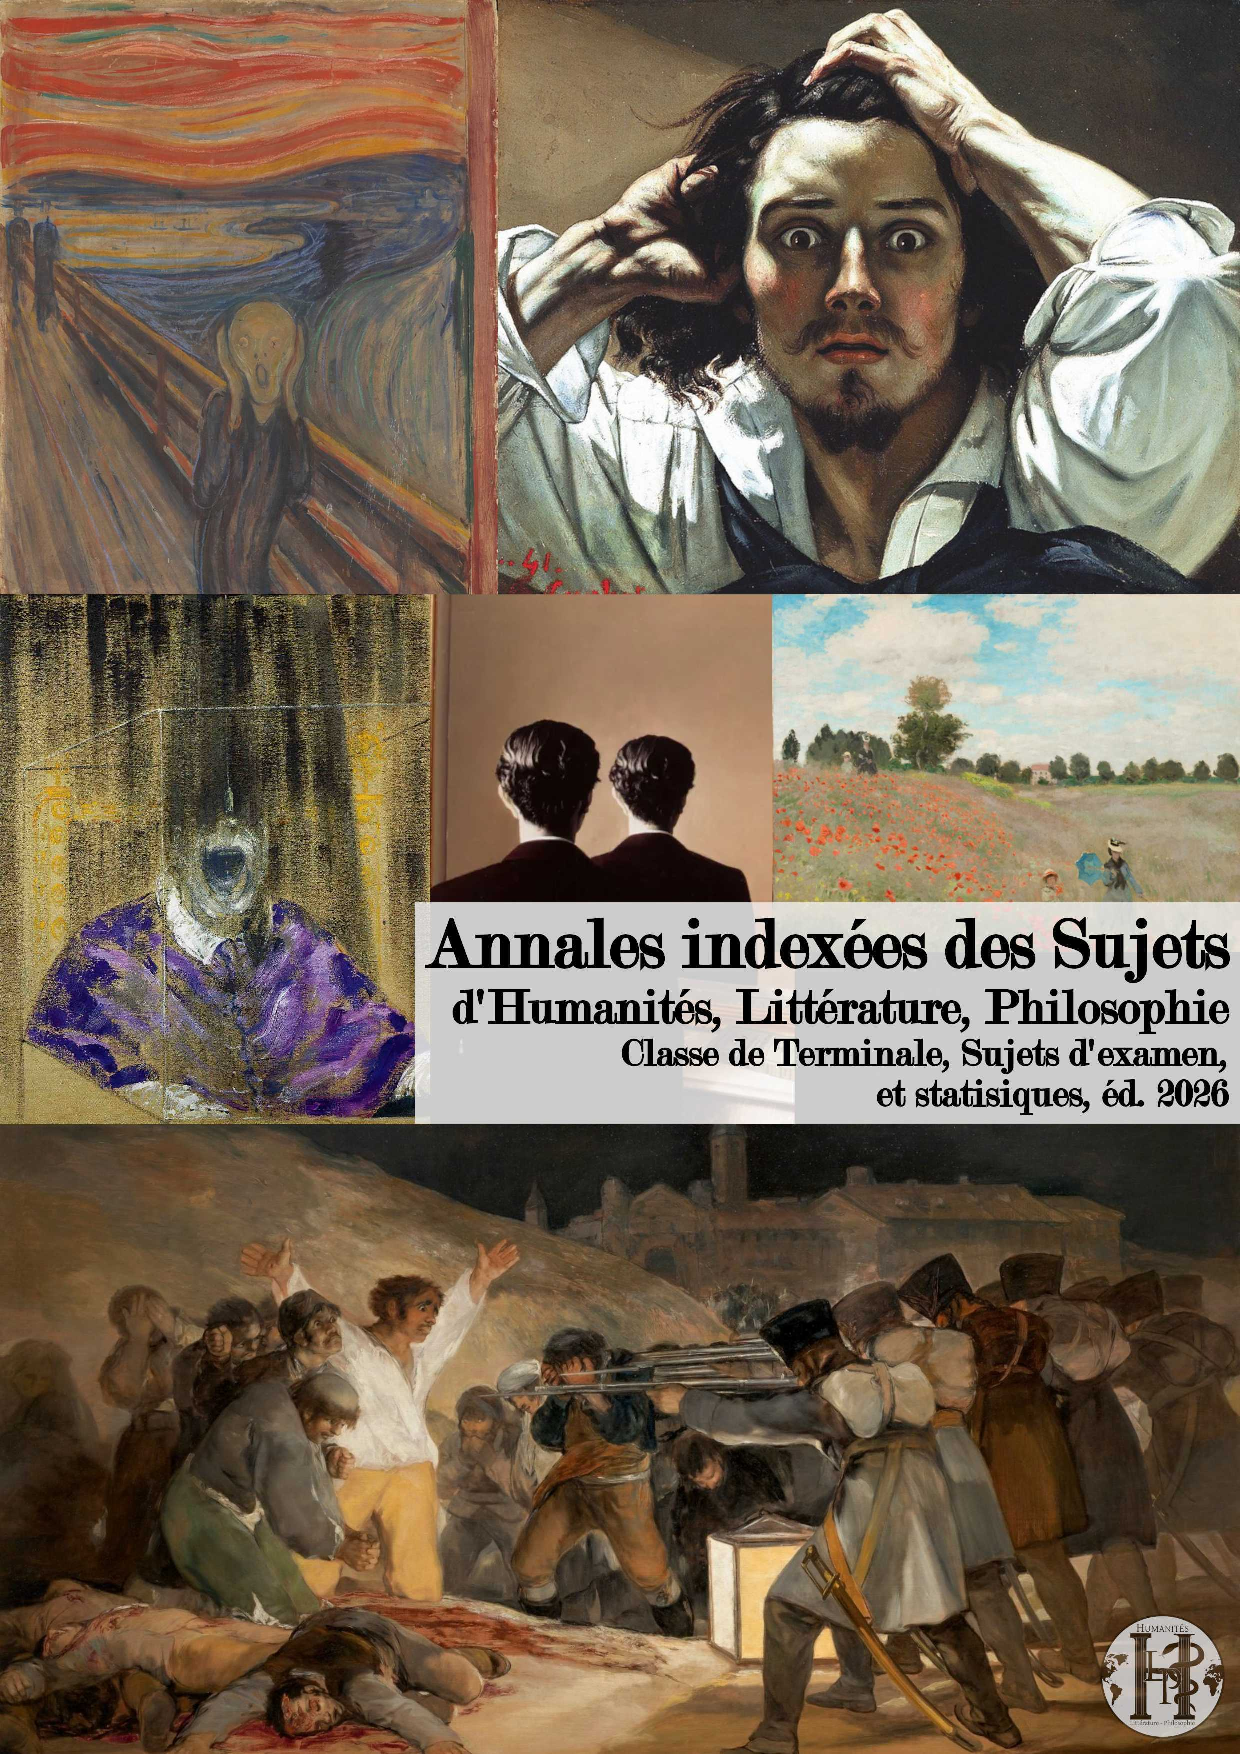
\includepdf{img/couv2026_sujetshlp-sanscorrTale.pdf}

\frontmatter

\input{titlepagesanscorr}

\clearpage
\pagestyle{plain}
\renewcommand{\headrulewidth}{0.0pt}
~

\vfill
\textbf{Images utilisées en couverture} :\vspace{6pt}

\setlength{\parskip}{3pt}
Edvard \textsc{Munch}, \textit{Le Cri} (\textit{Skrik}), 1893, tempera et pastel, 91~×~73.5~cm,  Musée national de l'Art, de l'Architecture et du Design (Oslo)  -- Image libre de droit (Wikimedia Commons).

Gustave \textsc{Courbet}, \textit{Le Désespéré}, 1843-1845, huile sur toile, \numprint{45}~×~\numprint{54}~cm, Collection privée, Conseil Investissement Art (BNP Paribas)  -- Image libre de droit (Wikimedia Commons).

Francis \textsc{Bacon}, \textit{Étude d'après le portrait du pape Innocent X par Velázquez} (\textit{Study after Velázquez's Portrait of Pope Innocent X}), 1953, huile sur toile, \numprint{153}~×~\numprint{118}~cm,  	
Des Moines Art Center (Des Moines, USA), \href{desmoinesregister.com}{desmoinesregister.com}.

René \textsc{Magritte}, \textit{La Reproduction interdite}, 1937, huile sur toile, \numprint{79}~×~\numprint{65,5}~cm, Musée Boijmans Van Beuningen (Rotterdam, Pays-Bas).

Claude \textsc{Monet}, \textit{Les Coquelicots}, 1873, huile sur toile, \numprint{50}~×~\numprint{65}~cm, Musée d'Orsay, (Paris) -- Image libre de droit (Wikimedia Commons).

Francisco \textsc{Goya}, \textit{Le trois mai} (\textit{Los fusilamientos del tres de mayo}), 1814, huile sur toile, \numprint{266}~×~\numprint{345}~cm, Musées du Prado (Madrid, Espagne)  -- Image libre de droit (Wikimedia Commons).

\vspace*{12pt}

\doclicenseIcon \doclicenseLongText
\setlength{\parskip}{6pt}
\clearpage

\bigskip

\fancypagestyle{normal}
\fancyhead{} % clear all header fields 
\fancyhead[RO]{Humanités, Littérature, Philosophie -- Banque des sujets indexés}
\fancyhead[LE]{\rightmark}
\fancyfoot{} %clear all footer fields
\fancyfoot[RO]{\textbf{\thepage} \hspace*{1.5cm}}
\fancyfoot[LE]{\hspace*{1.5cm}\textbf{\thepage}}
\renewcommand{\headrulewidth}{0.4pt}
\renewcommand{\footrulewidth}{0pt}

{\let\clearpage\relax%
\noindent\chapter{Avertissement}
}
\markright{Avertissement}{}
\label{avertissement}

Ce document vise à être un outil efficace pour l'ensemble des professeurs chargés d'enseigner
la spécialité «~Humanités, Littérature, Philosophie~». Il ne revêt aucun caractère officiel
et a été d'abord conçu pour simplifier le travail des professeurs, notamment par présence de différents index à la fin de ce document (à partir de la page \pageref{indexdeb}).

Si vous souhaitez accéder à une vision synoptique des différentes questions qui ont été posées, ainsi qu'aux sujets téléchargeables en version Word (.doc ou .docx) ou LibreOffice (.odt), vous pouvez vous rendre sur le Google Doc des \href{https://docs.google.com/document/d/1594BtSBMpnk_i"Lpqf7vzIPnFkFG6ZFvygOAMzdtbPhA/edit?usp=sharing}{Annales de sujets d'Audrey Pardigon}. Si vous souhaitez seulement avoir un fichier avec tous les sujets et un index des auteurs, vous les trouverez à \href{https://drive.google.com/file/d/1DnEUzL6_MTiRfS60gFycgNy-jxfQFMsu/view?usp=sharing}{ce lien} (odt) ou \href{https://docs.google.com/document/d/1XnJ397bNF5Vn-ZwEVjEvbJiCvbMBvRGi/edit?usp=sharing&ouid=103662385121242831300&rtpof=true&sd=true}{ce lien} (docx) (sans l'index des auteurs pour le fichier Word). Vous pouvez retrouver ce fichier et les fichiers qui ont servi à créer ce fichier (écrit en \LaTeX{}) \href{https://drive.google.com/drive/folders/1QwtvLY3i87WzyajRLPe0Xmmb31FK9oDp?usp=sharing}{ici}. Si vous souhaitez disposer d'une version de ce fichier avec les éléments d'évaluation, vous la trouverez ici~: \sujetshlpcorr{}.

\section*{Intégration des «~sujets zéro~» et ordre des sujets}
\phantomsection\addcontentsline{toc}{section}{«~Intégration des sujets zéro~» et ordre des sujets}

Quoiqu'ils n'aient pas fait l'objet d'une session d'examen, et qu'aucun élève n'ait donc composé sur ces sujets, on a intégré dans ces annales les «~sujets zéro ~», \cad{} les sujets proposés aux professeurs pour qu'ils se fassent une idée des attendus de l'examen. Ils ont été placés en premier pour chacun des grands thèmes de l'année de Terminale (la recherche de soi et l'humanité en question) et sont signalés, tant pour les index que pour le sujet lui-même, par le fait qu'on a indiqué «~Sujet 0 ~» comme centre d'examen. Ils peuvent ainsi être aisément distingués des autres sujets. Ce sont également les seuls sujets qui aient été publiés en 2020.

Pour l'ordre des sujets, on a procédé comme on avait déjà fait pour les \href{https://drive.google.com/file/d/1KN7gwAOkmIXFNAGYKYemD3y7Q0n68Phn/view?usp=sharing}{sujets de Première} en séparant les deux thèmes de l'année, de manière à permettre de naviguer plus aisément entre des sujets qui portent sur des thématiques similaires. On a pour chaque thématique classé les sujets par ordre chronologique d'année puis par ordre alphabétique du centre d'examen (Amérique du Nord, Amérique du Sud, Asie-Pacifique, Centres étrangers, La Réunion, Liban, Métropole, Nouvelle-Calédonie, Polynésie). Certains sujets n'ont parfois pas pu être retrouvés (à l'image des sujets du jour 1 pour les épreuves de spécialité du bac 2021 en Asie) ou n'ont jamais été publiés parce que les épreuves ont été totalement annulées, que ce soit en raison de l'épidémie de Covid-19 lors des sessions 2021 et 2022 ou pour des raisons politiques (les épreuves de spécialités ont ainsi été annulées en Nouvelle-Calédonie en 2021, et pour des raisons liées à la situation politique en 2024). Depuis 2022, les épreuves ayant lieu en-dehors de la Métropole sont de plus en plus regroupées par «~groupe ~» de Centres étrangers~: les épreuves de spécialités ont par exemple ainsi eu lieu au même moment en 2022 dans les Académies de Guadeloupe, Guyane, Mayotte, Martinique, Métropole et de la Réunion, ce qui explique l'absence de sujets spécifiques à la Réunion pour la session 2022. C'est aussi le cas du Liban en 2024 qui a rejoint les «~Centres étrangers gr.~1~».

\section*{Au sujet des index}
\phantomsection\addcontentsline{toc}{section}{Au sujet des index}

On trouvera à la fin, à partir de la page \pageref{indexdeb}, un \hyperlink{indexa}{index des auteurs} sur lesquels portent les sujets (p.~\pageref{indexa}), \hyperlink{indexg}{un index des textes selon leur genre} (p.~\pageref{indexg}), 
un \hyperlink{indexw}{index des questions selon les axes du programme puis selon leur type} (p.~\pageref{indexw}), ainsi qu'\hyperlink{indexv}{un index des questions selon leur type puis selon les thèmes du programme} (p.~\pageref{indexv}), \hyperlink{indexq}{un index général des questions selon leur type (interprétation ou réflexion et littéraire ou philosophique)} (p.~\pageref{indexq}), un \hyperlink{indexn}{index des sujets par lieux et années} (p.~\pageref{indexn}), qui permet de se faire une idée rapide des sujets proposés au fil des années et de retrouver l'ordre dans lequel les sujets ont été publiés,  ainsi qu'\hyperlink{indext}{un index des thèmes abordés par les textes}, qui permet de chercher rapidement un sujet sur un thème abordé en cours (p.~\pageref{indext}). Pour se repérer plus rapidement dans cet index, nous renvoyons à la \hyperlink{repere-thematique}{section proposant une liste de termes indexés} pour chaque chapitre et grandes thématiques au sein de chaque chapitre (p.~\pageref{repere-thematique}).

Plusieurs des index (concernant les axes du programme particulièrement, et concernant les genres des textes)
sont une simple proposition et n'engagent que moi.
J'ai essayé au mieux d'identifier le genre du texte, ce qui a parfois été difficile,
particulièrement pour les textes littéraires, dont je ne suis pas spécialiste.
Doit-on bien ranger l'ouvrage de Simone de Beauvoir, \textit{Mémoires d'une jeune fille rangée} dans la catégorie des autobiographies, quand cela a également une portée philosophique et qu'à certains égards on pourrait le considérer comme une forme d'apologie~? Que dire de l'ouvrage de Charlotte Delbo qui, certes, est le récit de l'expérience concentrationnaire de l'auteur, mais qui emploie une multitude de genres pour le faire~? Par nécessité j'ai tranché, mais cette catégorisation n'est pas absolue, et je serais heureux 
d'\href{mailto:mikael.quesseveur@ac-lille.fr}{avoir des retours}
et d'être corrigé.

On a essayé, de notre mieux, de rattacher chaque sujet aux grands axes de chaque semestre, la distinction entre les «~Expressions de la sensibilité~» et les «~Métamorphoses du moi~» étant néanmoins parfois poreuses, tout comme le rapport entre violence et technique qui rattache les «~Limites de l'humain~» à «~Histoire et violence~». Parfois, la classification est originale. Certains mêlent ainsi les deux semestres, à l'image du sujet d'essai littéraire sur le texte d'Hans Jonas (p.~\pageref{jonas-amérique2021}) sur la technique, qui interroge la capacité de la littérature à nous rendre sensible à l'importance de la nature, thématique qu'on aurait plutôt attendu autour des expressions de la sensibilité, mais qui n'a pris son sens qu'en considérant la question de la technique et de l'écologie. D'autres sujets semblent exiger des connaissances issues des cours de Première, à l'image des sujets portant sur un passage de \textit{Tristes tropiques} de Claude Lévi-Strauss (p.~\pageref{lévi-strauss-liban2022}) qui fait appel pour l'interprétation philosophique au concept de monde et à la question de la découverte, et pour l'essai littéraire à la question de la culture. Ce n'est qu'en tant que ce sujet se rapporte au concept d'humanité qu'il semble bien pouvoir se rapprocher explicitement de «~L'humanité en question ~», et que l'on peut certainement y voir une interrogation sur la modernité qui, à certains égards, introduit une pensée post-moderne qu'on peut rattacher aux «~Limites de l'humain ~».

Pour autant, cette catégorisation peut certainement être remise en question et je serais heureux d'\href{mailto:mikael.quesseveur@ac-lille.fr}{avoir des retours} et d'être corrigé. On remarquera d'ailleurs, qu'entre la première version et celle-ci, j'ai effectué certaines corrections, que l'on retrouvera dans les 
\hyperlink{errata}{Errata et corrections}.

\section*{Les statistiques}
\phantomsection\addcontentsline{toc}{section}{Les statistiques}

Puisqu'il commence à y avoir beaucoup de sujets, on a également, à partir du travail effectué, ajouté un chapitre de \hyperlink{statistiques}{Statistiques}, qui permet de se faire une idée rapide des sujets qui ont jusqu'à présent été proposés, de manière à en évaluer la répartition thématique notamment et les éventuelles affinités entre les types de sujets et les types de questions. Il convient de rester néanmoins très prudent~: «~Éducation, transmission, émancipation~»{} et «~Création, continuités et ruptures~»{} n'ayant pu faire l'objet d'une évaluation qu'à partir de la session 2024, il existe un écart important entre le nombre de sujets proposés sur ces deux chapitres et les autres~; l'écart est d'autant plus important que pendant la période du Covid, chaque jour étaient proposés deux sujets, et que «~Éducation, transmission, émancipation~»{} ni «~Création, continuités et ruptures~»{} ne pouvaient faire l'objet d'un sujet à ce moment.

Ces statistiques sont divisées en deux grands groupes :

\begin{enumerate}
\item D'abord les statistiques générales sur l'ensemble des sujets. On a ainsi détaillé selon les disciplines pour chaque chapitre le nombre de questions posées, en essayant de rendre l'ensemble le plus lisible possible. Pour rendre l'ensemble le plus efficace possible, les nombres dans le tableau renvoient désormais directement par un hyperlien à \hyperlink{indexv}{l'index selon les types de sujet puis selon les selon les axes du programme}, ce qui permet rapidement de faire la liste des questions posées pour chaque thème. Un troisième tableau résume l'ensemble des questions posées selon les thèmes, de manière plus compacte, et sans répéter les données\footnote{On a conservé les trois tableaux parce qu'il paraît utile pour un professeur, qui cherche à identifier le nombre de questions par axes du programme de manière précise de suivre la logique des chapitres du programme, en cherchant dans l'entrée pertinente du programme, ce que ne permet pas le tableau plus compacte, qui demande peut-être plus d'habitude pour être lu efficacement.} On a également inséré, à la suite une page qui résume, à l'aide de graphiques, la répartition des sujets selon les axes du programme. Ce dernier tableau et cette page de graphique sont repris dans les pages qui suivent pour les statistiques par centres d'examen.

\item Ensuite les statistiques par centres d'examen, classés par ordre alphabétique. Pour que ces statistiques soient suffisamment significatives, on a intégré que les centres d'examen dans lesquels il y a eu suffisamment de sujets proposés, pour que cela ait du sens à représenter graphiquement les données. On a essayé de rendre ces graphiques aussi lisibles que possibles, mais comme pour les tableaux précédents, il était nécessaire de faire appel aux acronymes que l'on utilise ailleurs. Il permet certainement en tout cas de se faire une idée rapide des tendances (passées) dans les différents centres d'examen.
\end{enumerate}

\section*{Corrections apportées aux sujets}
\phantomsection\addcontentsline{toc}{section}{Corrections apportées aux sujets}

Pour certains sujets, on s'est permis d'effectuer des corrections d'ordre typographique. Ainsi a-t-on pu mettre \textit{La Marseillaise} en italique dans le sujet portant sur \textit{14} de Jean Echenoz (Polynésie, 2021) ou encore mettre les majuscules qui conviennent à «~Première Guerre mondiale ~», conformément aux normes, dans l'intitulé du sujet d'interprétation philosophique portant sur le texte de Walter Benjamin, \textit{Expérience et pauvreté} (Amérique 2022). On a corrigé également une coquille manifeste dans le «~sujets 0 ~» portant sur une lettre de Jacques Rivière à Antonin Artaud. Dans le premier paragraphe, en effet, on a supprimé des guillemets qui étaient répétés deux fois~: \textcolor{darkgray}{«~qui du dehors attaque l’âme~»~»} est ainsi devenu \textcolor{darkgray}{«~qui du dehors attaque l’âme~»}. On a également modifié, selon les règles typographiques traditionnelles du français, la présentation des ordinaux de siècle, en plaçant en exposant l'abréviation du suffixe des adjectifs ordinaux, notamment pour le sujet portant sur Michel Foucault proposé en Métropole le jour 1 en 2021, ou encore dans les notes de bas de page du sujet proposé le deuxième jour en Polynésie en 2024. En-dehors de ces corrections typographiques et de la correction de la coquille, on n'a corrigé aucun texte des sujets. Pour les autres corrections, on pourra voir les corrections apportées à la précédente édition (notamment des coquilles) dans les \hyperlink{errata}{Errata et corrections}.

\section*{Remarques concernant les sujets et leur indexation}
\phantomsection\addcontentsline{toc}{section}{Remarques concernant les sujets}

Qu'on me permette ici d'insister sur le fait que l'indexation que je propose pour ces sujets n'a aucune valeur absolue ni officielle. Elle est très certainement contestable en bien des moments, et si j'ai essayé, au mieux, d'identifier le chapitre ou les chapitres de référence pour chaque question, il est possible que certains de mes choix ne soient pas les plus adéquats. N'hésitez pas à ce titre, si vous trouviez l'indexation de certains sujets contestables, à \href{mailto:mikael.quesseveur@ac-lille.fr}{me l'indiquer} pour que j'effectue les corrections nécessaires. Pour cette nouvelle édition, j'ai d'ailleurs moi-même changé l'indexation de certains sujets (ce qui est signalé dans \hyperlink{errata}{les \textit{errata} et corrections}.

À ce titre, il convient de rester prudent concernant les statistiques ou même le classement de ces sujets au sein de deux chapitres différents correspondant aux axes du programme~: ils sont l'effet de mes choix et n'ont aucune valeur en soi. Les statistiques, particulièrement, ne dépendent que du fait que j'ai indexé les sujets d'une certaine manière, et on obtiendrait certainement des résultats très différents avec une indexation différente. Concernant les sujets qui font appel à des connaissances des deux semestres, lorsqu'un des deux questions se référaient explicitement à un seul semestre, on a placé le sujet dans le chapitre correspondant. Quand cela n'était pas le cas, on a essayé d'identifier la thématique majeure du texte, et on a ainsi placé le sujet là où cela paraissait pertinent. Si les thématiques étaient trop intrinsèquement mêlées, on a généralement placé le sujet dans «~La recherche de soi~~». 

Puisque le nombre de sujets commence à devenir plus conséquent, il devient possible de faire quelques remarques qui permettent, peut-être, de mieux appréhender l'épreuve. On remarquera à ce titre quelques singularités. La première, et peut-être la plus instructive (et surprenante) réside dans le fait que deux textes identiques ont été proposés en 2023 en Nouvelle-Calédonie (Jour 1) et en Métropole (session de Remplacement, Jour 2), à savoir un texte de Joseph Ponthus extrait d'\textit{À la ligne, Feuillets d'usine}. Les deux sujets ne sont pas strictement identiques, puisqu'on ne trouve au v.~19 dans le sujet de Nouvelle-Calédonie aucune espace qui précède «~Tous les matins du monde ~», tandis que c'est le cas pour le sujet proposé en Métropole (v.~22 dans le sujet officiel). La numérotation des lignes y est également différente, puisque les marges semblent avoir été plus grandes pour le sujet de Métropole. Nous avons, pour la mise en page en général des vers, privilégié celle de Nouvelle-Calédonie, puisqu'il semblait alors que les retours à la ligne étaient moins dus à la disposition spécifique du sujet qu'à une reproduction du sujet (chaque vers commençant ainsi par une majuscule). Néanmoins, on a reproduit la différence entre les deux sujets quant à la présence de l'espacement. On remarquera également que les questions proposées n'étaient pas identiques, puisque le sujet calédonien propose comme question d'interprétation~: «~Comment s'exprime, dans ce texte, la violence de l'usine sur «~toutes les ouvrières et tous les ouvriers~~»~?~~», tandis que le sujet métropolitain propose~: «~«~Je suis là sans y être~~», dit le poète. En quoi cette phrase rend-elle compte du travail à l'usine tel qu'il est décrit dans ce texte~?~~». Pour les sujets de réflexion nous avons en Nouvelle-Calédonie~: «~Peut-on rester humain dans des conditions inhumaines~?~»  et en Métropole~: «~Le travail menace-t-il notre dignité~?~~». C'est l'occasion ainsi de comprendre que les questions posées ne sont pas rigidement attachées à chaque texte et qu'il est possible pour tout professeur de choisir une question qui lui paraîtrait pertinente pour préparer ses élèves au regard de son cours et de ce qu'il trouve intéressant dans un texte.

On trouve un phénomène relativement identique en Polynésie en 2022 avec un texte d'Hannah Arendt quasiment identique au sujet~0 proposé sur Hannah Arendt. En fait, seule la première phrase du texte du sujet~0 a été enlevée, et le reste du texte est commun. Les questions à nouveau sont différentes, et abordent, pour l'essai autant que pour la question d'interprétation, des dimensions radicalement différentes du texte ou de la pensée. Il est en ce sens envisageable que des sujets déjà proposés lors de sessions précédentes puissent faire, à nouveau, l'objet d'une épreuve avec des questions différentes.

\section*{Éléments d'évaluation}
\phantomsection\addcontentsline{toc}{section}{Éléments d'évaluation}

Cette version du fichier ne contient pas les éléments d'évaluation. Si vous souhaitez accéder à la version de ce fichier avec les éléments d'évaluation, vous pouvez vous rendre à ce lien \sujetshlpcorr{}.

À partir de l'édition 2025, on a proposé une indexation des sujets disposant d'éléments d'évaluation. Ces éléments d'évaluation n'ont pas de valeur prescriptive, mais permettent certainement d'une part d'identifier des références pertinentes pour les essais (et donc d'enrichir le cours) et d'autre part pour les questions d'interprétation de s'assurer que l'on a correctement identifié les éléments saillants d'un texte quant à son interprétation. Ils visent à être un guide pour les professeurs dans la correction des épreuves, et il nous paraissait en ce sens pertinent de les intégrer dans une version au moins de la banque indexée des sujets. On a ajouté, en plus de ces éléments d'évaluation un index des références culturelles mobilisées dans les éléments d'évaluation. L'ajout des éléments d'évaluation a le principal inconvénient d'allonger (très) largement le document : l'édition 2022 comptait au total 110~pages, tandis que l'édition comportant les éléments d'évaluation dépasse les 380~pages. Parce que \LaTeX{} est destiné à la manipulation de ce genre de documents, cela ne pose pas de difficultés dans la conception, mais il est possible à l'usage que cela ne soit pas idéal. Si vous préférez ce fichier à celui contentant les éléments d'évaluation, je suis intéressé par les raisons de vos préférences. N'hésitez pas, en ce sens, si vous utilisez cette banque de sujets, à \href{mailto:mikael.quesseveur@ac-lille.fr}{m'indiquer ce que vous en pensez}. Si vous souhaitez disposer d'un document avec les éléments d'évaluation vous le trouverez en cliquant sur ce lien~: \sujetshlpcorr{}.

\section*{Au sujet de ce PDF}
\phantomsection\addcontentsline{toc}{section}{Au sujet de ce PDF}

Le PDF que vous lisez a été fait sous \LaTeX{}, notamment en raison de la nécessité de disposer de plusieurs index
et des grandes possibilités offertes par ce langage pour l'automatisation d'un certain nombre de tâches
par l'utilisation des macros. Cela permettait, au demeurant, de rendre ce PDF «~interactif~», c'est-à-dire
que vous pouvez facilement naviguer au sein de ce PDF à l'aide des hyperliens cliquables qui s'y trouvent.
Vous trouverez également des signets (\textit{bookmarks}) qui vous permettent de naviguer facilement à partir du
panneau latéral de votre lecteur de PDF. Les liens sont indiqués par des textes avec une couleur différente~: en bleu les liens internes au document (présentés ainsi~: \textcolor{darkblue!80!black}{lien interne}) et en violet foncé les liens externes (présentés ainsi~: \textcolor{darkviolet!80!black}{lien externe}).
Les couleurs ont été choisies pour ne pas être (trop) visibles à l'impression tout en s'assurant qu'ils restent bien identifiables lors de la navigation dans le PDF.

On a conçu le document pour qu'il distingue les pages de gauche et de droite~: de la sorte on pourra aisément
l'imprimer en recto-verso.

Un mot enfin sur les droits de diffusion et de partage de ce fichier. Ce document et les fichiers \LaTeX{} qui
en sont à l'origine sont sous Licence Creative Commons : \doclicenseLongText{} Autrement dit vous êtes autorisés
à partager, distribuer et communiquer le matériel par tous moyens et sous tous formats ainsi qu'à adapter 
(c'est-à-dire à remixer, transformer, et créer) ce fichier à vos besoins pour toute utilisation non-commerciale.
Vous devez créditer l'Œuvre, intégrer un lien vers la licence et indiquer si des modifications ont été effectuées à
l'œuvre. Vous devez indiquer ces informations par tous les moyens raisonnables, sans toutefois suggérer que l'Offrant vous
soutient ou soutient la façon dont vous avez utilisé son œuvre. Vous n'êtes pas autorisé à faire un usage commercial de
cette œuvre, tout ou partie du matériel la composant. Dans le cas où vous effectuez un remix, que vous
transformez, ou créez à partir du matériel composant l'œuvre originale, vous devez diffuser l'œuvre modifiée dans les même
conditions, c'est à dire avec la même licence avec laquelle l'œuvre originale a été diffusée. Il va sans dire que les
fichiers de textes ne sont pas soumis à ces droits puisqu'ils appartiennent en partie au domaine public ou qu'ils sont des extraits d'œuvres sur lesquels je n'ai aucun droit. Par contre, l'utilisation du
code qui a permis la création de fichier est, lui, soumis à ces droits. À dire vrai ce n'est pas tant pour que mon
nom soit cité que je mets ce document sous Licence, mais pour éviter que mon travail ne soit commercialisé (qu'il
s'agisse du code ou de la première indexation des sujets que je propose). Pour autant, toute participation à 
l'amélioration de l'indexation est la bienvenue, et je vous engage à m'écrire à 
\href{mailto:mikael.quesseveur@ac-lille.fr}{cette adresse}.

\begin{flushright}M.~Q.\end{flushright}

\vfill{~}

\doclicenseImage

\clearpage

\pagestyle{plain}

\cleardoublepage

\pagestyle{ToC}

\setlength{\parskip}{0pt}
\phantomsection\addcontentsline{toc}{chapter}{Sommaire}
\shorttoc{Sommaire}{1}

\cleardoublepage

\setlength{\parskip}{6pt}

\mainmatter

\pagestyle{fancy}

\part{Sujets}

\chapitre{La recherche de soi}{img/Friedrich_voyageur.png}{Caspar David \textsc{Friedrich}, \textit{Le Voyageur contemplant une mer de nuages}, 1818, huile sur toile, 94.4×74.8cm, Hamburger Kunsthalle (Hambourg, Allemagne).}{0.6\textwidth}

\cleardoublepage

\sujetn{%
	nomauteur=Alain,
	prenomauteur=,
	initialeprenom =,
	particule=,
	titre = {Les idées et les âges},
	semestre = \RS,
	lieu = Sujet 0,
	annee = 2020,
	type = Non-proposé,
	jour = 0,
	datepub = 1927,
	ajoutref =,
	genre = \essaip,
	corrige =oui,
	liencorrige={sujet0_alain},
	typequn = \phil,
	typeqdeux = \litt,
	qun = {Comment Alain justifie-t-il l'idée d'une constitution inébranlable de la personnalité~?},
	qdeux ={«~Quelque chose qui ne peut changer~»~: la littérature libère-t-elle de l'assignation à une identité~?},
	themeprogrammequn=MM,
	themeprogrammeqdeux=MM}%
	{Un être humain nous jette d'abord au visage cette forme et cette
couleur, ce jeu des mouvements, qui ne sont qu'à lui. Les marques de
l'âge et du métier s'imprimeront sur cette écorce, mais sans la
changer. Tel il est à douze ans, sur les bancs de l'école, tel il
sera~; pas un pli des cheveux n'en sera changé. La manière de
s'asseoir, de prendre, de tourner la tête, de s'incliner, de se
redresser, est dans cette forme pour toute la vie. Ce sont des signes
constants, que l'individu ne cesse point de lancer, ni les autres
d'observer et de reconnaître. Quelque puissance de persuasion que
j'aie, que je sois puissant ou riche, ou flatteur, ou prometteur, je
sais bien qu'il ne changera rien de ce front large ou étroit, de
cette mâchoire, de ces mains, de ce dos, pas plus qu'il ne changera
la couleur de ces yeux. Alexandre, César, Louis XIV, Napoléon, ne
pouvaient rien sur ces différences. Aussi l'attention de tout homme
se jette là, assurée de pouvoir compter sur cette forme si bien
terminée, si bien assise sur elle-même, si parfaitement composée, où
tout s'accorde et se soutient. On peut le tuer, on ne peut le
changer. Là-dessus donc s'appuient d'abord tous nos projets et toutes
nos alliances. Vainement l'homme tend un autre rideau de signes,
ceux-là communs, qui sont costumes, politesses, phrases~; tout cela
ne brouille même pas un petit moment le ferme contour, la couleur,
l'indicible mouvement, le fond et le roc d'une nature. Ici est
signifié quelque chose qui ne peut changer et qui ne peut tromper.
Mais quoi~?
\theme{identité!personnelle}\theme{personnalité}\theme{identité}\theme{apparences}\theme{vanité}\theme{corps}}

%%%%%%%%%%%%%%%%%%%%%%%%%%%%Nv-Sujet%%%%%%%%%%%%%%%%%%%%%%%%%%%%%%%%%%%%%%%%%%
\sujetn{%
	nomauteur = Riviere,
	prenomauteur = Jacques,
	initialeprenom = J,
	particule=,
	titre = {Lettre à Antonin Artaud du 8 juin 1924},
	semestre = \RS,
	lieu = Sujet 0,
	annee = 2020,
	type = Non-proposé,
	jour = 0,
	datepub = 1924,
	ajoutref =,
	genre = \lettrel,
	corrige =Oui,
	liencorrige={sujet0_riviere},
	typequn = \litt,
	typeqdeux = \phil,
	qun = {En quoi la réflexion de Jacques Rivière expose-t-elle les déchirements du Moi~?},
	qdeux ={Parvient-on jamais à être soi-même~?},
	themeprogrammequn=MM,
	themeprogrammeqdeux=MM}
	{\chapeau{En 1923, Antonin Artaud a expédié des poèmes à \emph{La nouvelle revue française}. Son directeur, Jacques Rivière, ne souhaite pas les
publier, mais s'en explique, et ouvre ainsi une correspondance suivie
entre les deux écrivains.}

Vous dites «~qu'un homme ne se possède que par éclaircies, et même
quand il se possède, il ne s'atteint pas tout à fait~». Cet homme,
c'est vous~; mais je peux vous dire que c'est moi aussi. Je ne
connais rien qui ressemble à vos «~tornades~», ni à cette «~volonté
méchante~» qui «~du dehors attaque l'âme~» et ses pouvoirs
d'expression. Mais pour être plus générale, moins douloureuse, la
sensation que j'ai parfois de mon infériorité à moi-même n'est pas
moins nette.

Comme vous j'écarte, pour expliquer les alternatives par lesquelles je
passe, le symbole commode de l'inspiration. Il s'agit de quelque
chose de plus profond, de plus «~substantiel~», si j'ose détourner ce
mot de son sens, qu'un bon vent qui me viendrait, ou non, du fond de
l'esprit~; il s'agit de degrés que je parcours dans ma propre
réalité. Non pas volontairement, hélas~! mais de façon purement
accidentelle.

Il y a ceci de remarquable que le fait même de mon existence, comme
vous le notez pour vous-même, ne fait à aucun moment pour moi l'objet
d'un doute sérieux~; il me reste toujours quelque chose de moi, mais
c'est bien souvent quelque chose de pauvre, de malhabile, d'infirme
et presque de suspect. Je ne perds pas à ces moments toute idée de ma
réalité complète~; mais quelquefois tout espoir de la reconquérir
jamais. Elle est comme un toit au-dessus de moi qui resterait en
l'air par miracle, et jusqu'auquel je ne verrais aucun moyen de me
reconstruire.

Mes sentiments, mes idées – les mêmes qu'à l'habitude – passent en moi
avec un petit air fantastique~; ils sont tellement affaiblis,
tellement hypothétiques qu'ils ont l'air de faire partie d'une pure
spéculation philosophique, ils sont encore là, pourtant, mais ils me
regardent comme pour me faire admirer leur absence.

Proust a décrit «~les intermittences du cœur~»~; il faudrait
maintenant décrire les intermittences de l'être.

[…] En tout cas, c'est un fait, je crois, que toute une catégorie
d'hommes est sujette à ces oscillations du niveau de l'être. Combien
de fois, nous plaçant machinalement dans une attitude psychologique
familière, n'avons-nous pas découvert brusquement qu'elle nous
dépassait, ou plutôt que nous lui étions devenus subrepticement
inégaux~! Combien de fois notre personnage le plus habituel ne nous
est-il pas apparu tout à coup factice, et même fictif, par l'absence
des ressources spirituelles, ou «~essentielles~», qui devaient
l'alimenter~?

Où passe, et d'où revient notre être, que toute la psychologie jusqu'à nos jours a feint de considérer comme une constante~?
\theme{identité}\theme{identité!et différences}\theme{substance}\theme{soi!difficile accès à soi}\theme{moi!mobilité du moi}\theme{habitude}\theme{sentiments}}

%%%%%%%%%%%%%%%%%%%%%%%%%%%%Nv-Sujet%%%%%%%%%%%%%%%%%%%%%%%%%%%%%%%%%%%%%%%%%%
\sujetn{%
	nomauteur=Guéhenno,
	prenomauteur=Jean,
	initialeprenom =J,
	particule=,
	titre = {Carnets du vieil écrivain},
	semestre = \RS,
	lieu = {Amérique du Nord},
	annee = 2021,
	type =,
	jour =1,
	datepub = 1971,
	ajoutref =,
	genre = \autobiographie,
	corrige =Oui,
	liencorrige={amnord_2021_1_1},
	typequn = \phil,
	typeqdeux = \litt,
	qun = {Pourquoi, selon Jean Guéhenno, la vraie lecture commence quand on lit «~pour se trouver~»~?},
	qdeux ={Quels bénéfices le lecteur peut-il tirer de la fréquentation des
œuvres littéraires~?},
	themeprogrammequn=MM,
	themeprogrammeqdeux=EXSMM}%
	{\vspace*{6pt}\par
	Bien des gens ne lisent que pour éloigner l'ennui, comme ils écoutent
la radio, regardent la «~télé~», les images, ou feuillettent les
journaux. L'imprimé pullule et on pourrait dire, après tout, que les
gens n'ont jamais tant lu. Mais il y a lire et lire. La vraie lecture
commence quand on ne lit plus seulement pour se distraire et se fuir,
mais pour se trouver. Il y a un jour où tout inconsciemment on passe
de l'un à l'autre. Ce peut n'être pas volontaire, mais l'effet du
plaisir même, d'une sorte d'envoûtement dont un livre, qu'on tient
dans ses mains et qu'on ne peut plus quitter, est la cause. Ce n'est
pas non plus encore lire que de lire pour apprendre, pour savoir,
pour s'informer, et pour des raisons professionnelles.
Joubert\footnote{Moraliste français (1754-1824)} disait que «~notre
sort est d'admirer et non pas de savoir~». La vraie lecture est la
chose la plus intime et la plus désintéressée, encore qu'il ne s'y
agisse que de nous-mêmes.

C'est un temps qu'on se donne pour ne plus vivre par influence, par
contagion, mais pour reconnaître, choisir son propre chemin et
devenir soi-même. Un livre est un outil de liberté. Nous y découvrons
la vie d'un autre, soit l'auteur, soit l'un des personnages qu'il a
créés, et nous l'examinons avec une bien autre insistance et une bien
autre loyauté que la nôtre propre, et ainsi devenons-nous un peu
autres nous-mêmes sans y prendre garde. Un livre est un objet devant
soi, quelque chose sur quoi on peut réfléchir, à quoi on peut
revenir, qu'on peut corriger, contredire, discuter, quelque chose
qu'on juge. Les images, les sons passent aussi vite que les moments
successifs de la vie. Un écrit, un livre reste. Il faut devant lui
dire oui ou non. Il fallait autrefois, pour former un homme, le tirer
de son silence et lui faire entendre le chant du monde autour de lui.
Il faut peut-être autant aujourd'hui le ramener à son silence, le
sauver du bruit et le reconduire à la solitude. Un livre est une
conversation et tout ensemble cependant un exercice de solitude. Je
veux ici écarter l'anecdote toute personnelle, mais je repense
souvent à ces nuits de mon adolescence, durant lesquelles je me
battais avec le destin\footnote{Jean Guéhenno évoque, à travers cette
expression, les années difficiles d'une enfance et d'une adolescence
marquées par la pauvreté.} et découvrais dans les livres ce que
pouvait être une vie libre par opposition à celle que je subissais.
Lit-on un grand roman~? On s'identifie à son héros. On y vit par
procuration. Et cela devient plus conscient, et vient le moment où on
ne lit plus pour aucun intérêt, pour aucun profit, rien que pour
«~admirer~», en toute gratuité et dans une joie indéfinissable,
au-delà de soi-même. Dès lors, on devient de plus en plus difficile.
On ne supporte plus les fantômes d'auteurs, les fantômes d'ouvrages.
Mais un vrai livre est devenu la chose la plus précieuse. Un homme
vous parle et il vous semble qu'il dise précisément ce que vous
attendiez, ce que vous vouliez dire mais n'auriez jamais su dire.
C'est tout simple et merveilleusement étrange. Ces mots, qui sont
aussi vos mots, comme par l'effet d'un charme, sont doués soudain
d'un nouveau pouvoir, et vous êtes curieusement débarrassé de
vous-même et devenu un autre, plus fin, plus délicat, plus profond
que vous-même. Vous êtes dans le monde où vous aimeriez vivre, mais
vous n'aviez jamais imaginé qu'il pût être si beau.
\theme{lecture}\theme{introspection!se trouver}\theme{intime}\theme{temps}\theme{autrui}\theme{solitude}\theme{silence}\theme{liberté}\theme{identité}}

%%%%%%%%%%%%%%%%%%%%%%%%%%%Nv-Sujet%%%%%%%%%%%%%%%%%%%%%%%%%%%%%%%%%%%%%%%%%%

\sujetn{%
	nomauteur=Duras,
	prenomauteur=Marguerite,
	initialeprenom =M,
	particule=,
	titre = {La Douleur},
	semestre = \RS,
	lieu = Amérique du Nord,
	annee = 2021,
	type =,
	jour =2,
	datepub = 1985,
	ajoutref =,
	genre = \romanl,
	corrige =Oui,
	liencorrige={amnord_2021_2_1},
	typequn=\litt,
	typeqdeux = \phil,
	qun = {Comment l'écriture de Duras rend-elle compte de la fragmentation du
moi~?},
	qdeux ={Dans quelle mesure la souffrance transforme-t-elle le sujet~?},
	themeprogrammequn=MM,
	themeprogrammeqdeux=EXSMM}
	{\chapeau{Dans \emph{La Douleur}, récit en forme de journal, Marguerite Duras
narre l'attente et le retour de son mari, nommé ici Robert L., des
camps de concentration.}

J'ai entendu des cris retenus dans l'escalier, un remue-ménage, un
piétinement. Puis des claquements de portes et des cris. C'était ça.
C'était eux qui revenaient d'Allemagne.

Je n'ai pas pu l'éviter. Je suis descendue pour me sauver dans la rue.
Beauchamp et D. le soutenaient par les aisselles. Ils étaient arrêtés
au palier du premier étage. Il avait les yeux levés.

Je ne sais plus exactement. Il a dû me regarder et me reconnaître et
sourire. J'ai hurlé que non, que je ne voulais pas voir. Je suis
repartie, j'ai remonté l'escalier. Je hurlais, de cela je me
souviens. La guerre sortait dans des hurlements. Six années sans
crier. Je me suis retrouvée chez des voisins. Ils me forçaient à
boire du rhum, ils me le versaient dans la bouche. Dans les cris.

Je ne sais plus quand je me suis retrouvée devant lui, lui, Robert L.
Je me souviens des sanglots partout dans la maison, que les
locataires sont restés longtemps dans l'escalier, que les portes
étaient ouvertes. On m'a dit après que la concierge avait décoré
l'entrée pour l'accueillir et que dès qu'il était passé, elle avait
tout arraché et qu'elle, elle s'était enfermée dans sa loge,
farouche, pour pleurer.

\bigskip

Dans mon souvenir, à un moment donné, les bruits s'éteignent et je le
vois. Immense. Devant moi. Je ne le reconnais pas. Il me regarde. Il
sourit. Il se laisse regarder. Une fatigue surnaturelle se montre
dans son sourire, celle d'être arrivé à vivre jusqu'à ce moment-ci.
C'est à ce sourire que tout à coup je le reconnais, mais de très
loin, comme si je le voyais au fond d'un tunnel. C'est un sourire de
confusion. Il s'excuse d'en être là, réduit à ce déchet. Et puis le
sourire s'évanouit. Et il redevient un inconnu. Mais la connaissance
est là, que cet inconnu c'est lui, Robert L., dans sa totalité.

\bigskip

Il avait voulu revoir la maison. On l'avait soutenu et il avait fait
le tour des chambres. Ses joues se plissaient mais elles ne se
décollaient pas des mâchoires, c'était dans ses yeux qu'on avait vu
son sourire. Quand il était passé dans la cuisine, il avait vu le
clafoutis qu'on lui avait fait. Il a cessé de sourire~: «~Qu'est-ce
que c'est~?~» On le lui avait dit. A quoi il était~? Aux cerises,
c'était la pleine saison. «~Je peux en manger~? – Nous ne le savons
pas, c'est le docteur qui le dira.~» Il était revenu au salon, il
s'était allongé sur le divan. «~Alors je ne peux pas en manger~? –
Pas encore. – Pourquoi~? – Parce qu'il y a déjà eu des accidents dans
Paris à trop vite faire manger les déportés au retour des camps.~»

Il avait cessé de poser des questions sur ce qui s'était passé pendant
son absence. Il avait cessé de nous voir. Son visage s'était
recouvert d'une douleur intense et muette parce que la nourriture lui
était encore refusée, que ça continuait comme au camp de
concentration. Et comme au camp, il avait accepté en silence. Il
n'avait pas vu qu'on pleurait. Il n'avait pas vu non plus qu'on
pouvait à peine le regarder, à peine lui répondre.

\bigskip

Le docteur est arrivé. Il s'est arrêté net, la main sur la poignée,
très pâle. Il nous a regardés puis il a regardé la forme sur le
divan. Il ne comprenait pas. Et puis il a compris~: cette forme
n'était pas encore morte, elle flottait entre la vie et la mort et on
l'avait appelé, lui, le docteur, pour qu'il essaye de la faire vivre
encore. Le docteur est entré. Il est allé jusqu'à la forme et la
forme lui a souri. Ce docteur viendra plusieurs fois par jour pendant
trois semaines, à toute heure du jour et de la nuit. Dès que la peur
était trop grande, on l'appelait, il venait. Il a sauvé Robert L. Il
a été lui aussi emporté par la passion de sauver Robert L. de la
mort. Il a réussi.
\theme{camp de concentration}\theme{souvenir}\theme{moi!fragmentation du moi} \theme{reconnaissance}\theme{autrui}\theme{autrui!comme inconnu}\theme{souffrance}\theme{temps}\theme{vie (et mort)}\theme{Shoah}}

%%%%%%%%%%%%%%%%%%%%%%%%%%%Nv-Sujet%%%%%%%%%%%%%%%%%%%%%%%%%%%%%%%%%%%%%%%%%%

\sujetn{%
	nomauteur=Thoreau,
	prenomauteur=Henry David,
	initialeprenom =H.~D,
	particule=,
	titre = {Walden ou la Vie dans les bois},
	semestre = \RS,
	lieu = Asie,
	annee = 2021,
	type =,
	jour =2,
	datepub = 1854,
	ajoutref =\linebreak traduction de Brice \textsc{Matthieussent},
	genre = \romanp,
	corrige =,
	liencorrige={asi_2021_2_1},
	typequn = \phil,
	typeqdeux = \litt,
	qun = {Comment Thoreau montre-t-il que l'attention aux choses sensibles
suffit à remplir l'existence~?},
	qdeux ={Les œuvres littéraires renouvellent-elles notre approche du quotidien~?},
	themeprogrammequn=EXS,
	themeprogrammeqdeux=EXS}
	{\vspace*{-27pt}\par
\chapeau{David Thoreau, écrivain et philosophie américain, a développé une
critique de la civilisation urbaine et industrielle. Il a aussi
choisi, à un certain moment de sa vie, de se retirer au fond des
bois.}

\vspace*{-7pt}Chacun doit trouver en lui-même son propre rythme, et c'est la vérité.
Le jour naturel est très calme et il ne reprochera jamais à quiconque
son indolence. Mon mode de vie me fournissait du moins cet avantage
sur ceux qui étaient contraints d'aller chercher ailleurs leurs
distractions, dans la société et au théâtre, car ma vie elle-même
était devenue ma distraction et elle ne cessait jamais de se
renouveler. C'était un drame aux nombreuses scènes, et sans fin. Si
vraiment nous trouvions toujours de quoi vivre et réglions sans cesse
notre existence selon la dernière et meilleure façon que nous avons
apprise, jamais nous ne connaîtrions l'ennui. Suivez votre génie
d'assez près, il ne manquera pas de vous montrer à chaque heure une
perspective inédite. Les tâches domestiques étaient un agréable
passe-temps. Quand mon sol était sale, je me levais de bonne heure,
j'installais tout mon mobilier dehors sur l'herbe, le lit et la
literie en vrac, je jetais de l'eau sur mon plancher, j'y répandais
du sable blanc venant du lac, puis je le frottais avec un balai pour
le rendre propre et immaculé~; et à l'heure où les villageois
prenaient leur petit-déjeuner, le soleil du matin avait suffisamment
séché ma maison pour me permettre d'y réemménager, et c'est à peine
si mes méditations s'en trouvaient interrompues. J'avais plaisir à
voir tous mes meubles et mes objets dehors dans l'herbe, faisant un
petit tas comme le ballot d'un bohémien, et ma table à trois pieds
d'où je n'ôtais pas les livres, la plume et l'encrier, dressée parmi
les pins et les hickories\footnote{«~hickories~»~: arbres d'Amérique
du Nord}. Ils semblaient heureux de prendre l'air, et presque
réticents à l'idée de réintégrer leur décor initial. Parfois, j'avais
envie d'installer un auvent au-dessus d'eux et de m'asseoir dessous.
Cela valait vraiment la peine de voir le soleil briller sur toutes
ces choses et d'entendre le vent souffler librement sur elles~; nos
objets les plus familiers semblent tellement plus intéressants quand
ils sont dehors que dans la maison. Un oiseau est perché sur la
branche toute proche, l'immortelle pousse sur la table et les ronces
s'enroulent autour de ses pieds~; les pommes de pin, les bogues de
châtaignes et les feuilles de fraisier jonchent l'herbe. On dirait
que c'est la manière dont ces formes ont été métamorphosées en
meubles, tables, chaises et lits – parce qu'ils ont été un jour parmi
elles.
\theme{introspection!se trouver}\theme{divertissement}\theme{nature!environnement}\theme{paysage}\theme{contemplation}\theme{regard!nouveau regard sur le monde}}

%%%%%%%%%%%%%%%%%%%%%%%%%%%%Nv-Sujet%%%%%%%%%%%%%%%%%%%%%%%%%%%%%%%%%%%%%%%%%%

\sujetn{%
	nomauteur=Balzac,
	prenomauteur=Honoré,
	initialeprenom =H,
	particule=de,
	titre = {Le Lys dans la vallée},
	semestre = \RS,
	lieu = Centres étrangers,
	annee = 2021,
	type =,
	jour =1,
	datepub = 1836,
	ajoutref =,
	genre = \romanl,
	corrige =,
	liencorrige={cea_2021_1_1},
	typequn=\litt,
	typeqdeux = \phil,
	qun = {Quels rôles joue le paysage dans l'expression de la sensibilité du
narrateur~?},
	qdeux ={La nature me parle-t-elle de moi~?},
	themeprogrammequn=EXS,
	themeprogrammeqdeux=EXS}
	{\chapeau{Félix, le personnage principal du roman, est l'amant de Henriette de
Mortsauf. Cette dernière est tiraillée entre son amour pour lui, et
celui, éperdu, qu'elle porte à ses enfants.}

«~J'avais oublié de vous rendre cette clef, lui dis-je en souriant.

—~Vous ne reviendrez donc plus~? dit-elle.

—~Est-ce que nous nous quittons~?~» demandai-je en lui jetant un
regard qui lui fit abaisser ses paupières pour voiler sa muette
réponse.

Je partis après quelques moments passés dans une de ces heureuses
stupeurs des âmes arrivées là où finit l'exaltation et où commence la
folle extase. Je m'en allai d'un pas lent, en me retournant sans
cesse. Quand au sommet du plateau je contemplai la vallée une
dernière fois, je fus saisi du contraste qu'elle m'offrit en la
comparant à ce qu'elle était quand j'y vins~: ne verdoyait-elle pas,
ne flambait-elle pas alors comme flambaient, comme verdoyaient mes
désirs et mes espérances~? Initié maintenant aux sombres et
mélancoliques mystères d'une famille, partageant les angoisses d'une
Niobé chrétienne\footnote{«~angoisses d'une Niobé chrétienne~»~: craintes d'une mère de perdre ses enfants}, triste comme elle, l'âme rembrunie, je trouvais
en ce moment la vallée au ton de mes idées. En ce moment les champs
étaient dépouillés, les feuilles des peupliers tombaient, et celles
qui restaient avaient la couleur de la rouille~; les pampres\footnote{«~pampres~»~: branches de vigne}
étaient brûlés, la cime des bois offrait les teintes graves de cette
couleur tannée que jadis les rois adoptaient pour leur costume et qui
cachait la pourpre du pouvoir sous le brun des chagrins. Toujours en
harmonie avec mes pensées, la vallée où se mouraient les rayons
jaunes d'un soleil tiède me présentait encore une vivante image de
mon âme. Quitter une femme aimée est une situation horrible ou
simple, selon les natures~; moi je me trouvai soudain comme dans un
pays étranger dont j'ignorais la langue~; je ne pouvais me prendre à
rien, en voyant des choses auxquelles je ne sentais plus mon âme
attachée. Alors l'étendue de mon amour se déploya, et ma chère
Henriette s'éleva de toute sa hauteur dans ce désert où je ne vécus
que par son souvenir.
\theme{paysage}\theme{nature!environnement}\theme{amour}\theme{souvenir}}

%%%%%%%%%%%%%%%%%%%%%%%%%%%%Nv-Sujet%%%%%%%%%%%%%%%%%%%%%%%%%%%%%%%%%%%%%%%%%%

\sujetn{%
	nomauteur=Bergson,
	prenomauteur=Henri,
	initialeprenom =H,
	particule=,
	titre = {Le Rire},
	semestre = \RS,
	lieu =Centres étrangers,
	annee =2021,
	type =,
	jour =2,
	datepub = 1900,
	ajoutref =,
	genre =\essaip,
	corrige =,
	liencorrige={cea_2021_2_2},
	typequn = \phil,
	typeqdeux = \litt,
	qun = {Selon ce texte, en quoi l'imagination poétique révèle-t-elle les
richesses du moi~?},
	qdeux ={L'expérience littéraire est-elle un effort d'observation intérieure~?},
	themeprogrammequn=EXSMM,
	themeprogrammeqdeux=EXSMM}
	{Notre caractère est l'effet d'un choix qui se renouvelle sans cesse.
Il y a des points de bifurcation (au moins apparents) tout le long de
notre route, et nous apercevons bien des directions possibles,
quoique nous n'en puissions suivre qu'une seule. Revenir sur ses pas,
suivre jusqu'au bout les directions entrevues, en cela paraît
consister précisément l'imagination poétique. Je veux bien que
Shakespeare n'ait été ni Macbeth, ni Hamlet, ni Othello~; mais il eût
été ces personnages divers si les circonstances, d'une part, le
consentement de sa volonté, de l'autre, avaient amené à l'état
d'éruption violente ce qui ne fut chez lui que poussée intérieure.
C'est se méprendre étrangement sur le rôle de l'imagination poétique
que de croire qu'elle compose ses héros avec des morceaux empruntés à
droite et à gauche autour d'elle, comme pour coudre un habit
d'Arlequin. Rien de vivant ne sortirait de là. La vie ne se recompose
pas. Elle se laisse regarder simplement. L'imagination poétique ne
peut être qu'une vision plus complète de la réalité. Si les
personnages que crée le poète nous donnent l'impression de la vie,
c'est qu'ils sont le poète lui-même, le poète multiplié, le poète
s'approfondissant lui-même dans un effort d'observation intérieure si
puissant qu'il saisit le virtuel dans le réel et reprend, pour en
faire une œuvre complète, ce que la nature laissa en lui à l'état
d'ébauche ou de simple projet.
\theme{caractère}\theme{personnage}\theme{imagination}\theme{introspection}\theme{art}\theme{virtuel}}


%%%%%%%%%%%%%%%%%%%%%%%%%%%%Nv-Sujet%%%%%%%%%%%%%%%%%%%%%%%%%%%%%%%%%%%%%%%%%%

\sujetn{%
	nomauteur=Foucault,
	prenomauteur=Michel,
	initialeprenom =M,
	particule=,
	titre = {Rêve et existence},
	semestre = \RS,
	lieu =Métropole,
	annee =2021,
	type =Candidats libres,
	jour =1,
	datepub = 1954,
	ajoutref = {«~Introduction~» de Michel Foucault dans l'ouvrage de Ludwig \textsc{Binswanger}},
	genre =\essaip,
	corrige =,
	liencorrige={metcal_2021_1_1},
	typequn = \phil,
	typeqdeux = \litt,
	qun = {En quoi l'expérience du rêve est-elle une expérience de soi~?},
	qdeux ={Qu'est-ce que la littérature partage avec le chaos des rêves~?},
	themeprogrammequn=MM,
	themeprogrammeqdeux=EXSMM}
	{Le sujet du rêve ou la première personne onirique, c'est le rêve
lui-même, c'est le rêve tout entier. Dans le rêve tout dit «~je~»,
même les objets et les bêtes, même l'espace vide, même les choses
lointaines et étranges, qui en peuplent la fantasmagorie. Le rêve,
c'est l'existence se creusant en espace désert, se brisant en chaos,
éclatant en vacarme, se prenant, bête ne respirant plus qu'à peine,
dans les filets de la mort. Le rêve, c'est le monde à l'aube de son
premier éclatement quand il est encore l'existence elle-même et qu'il
n'est pas déjà l'univers de l'objectivité. Rêver n'est pas une autre
façon de faire l'expérience d'un autre monde, c'est pour le sujet qui
rêve la manière radicale de faire l'expérience de son monde, et si
cette manière est à ce point radicale, c'est que l'existence ne s'y
annonce pas comme étant le monde. Le rêve se situe à ce moment ultime
où l'existence est encore son monde, aussitôt au-delà, dès l'aurore
de l'éveil, déjà elle ne l'est plus. C'est pourquoi l'analyse du rêve
est décisive pour mettre au jour les significations fondamentales de
l'existence.
\theme{rêve}\theme{sujet}\theme{imagination}\theme{monde}\theme{psychanalyse}\theme{inconscient}}

%%%%%%%%%%%%%%%%%%%%%%%%%%%%Nv-Sujet%%%%%%%%%%%%%%%%%%%%%%%%%%%%%%%%%%%%%%%%%%

\sujetn{%
	nomauteur=Tocqueville,
	prenomauteur={Alexis},
	initialeprenom ={A},
	particule=de,
	titre = {Souvenirs},
	semestre = \RS,
	lieu = Métropole,
	annee = 2021,
	type = Candidats libres,
	jour = 2,
	datepub = 1850-1851,
	ajoutref =,
	genre =\memoire,
	corrige =,
	liencorrige={metcal_2021_2_1},
	typequn = \phil,
	typeqdeux = \litt,
	qun = {À quels obstacles se heurte, selon Tocqueville, l'exigence de
sincérité~?},
	qdeux ={«~On est trop proche de soi pour bien voir~». La littérature permet de trouver le recul nécessaire pour «~bien parler de soi~»~?},
	themeprogrammequn=MM,
	themeprogrammeqdeux=MM}
	{Je voudrais bien rechercher ici les raisons qui me déterminèrent
alors, et, les ayant retrouvées, les exposer sans détour~; mais qu'il
est difficile de bien parler de soi~! J'ai observé que la plupart de
ceux qui ont laissé des Mémoires ne nous ont bien montré leurs
mauvaises actions ou leurs penchants que quand, par hasard, ils les
ont pris pour des prouesses ou de bons instincts, ce qui est arrivé
quelquefois. C'est ainsi que le \textit{cardinal de Retz}, pour
atteindre à ce qu'il considère comme la gloire d'avoir été un bon
conspirateur, nous avoue ses projets d'assassiner Richelieu, et nous
raconte ses dévotions et ses charités hypocrites de peur de ne point
passer pour un habile homme. Ce n'est pas alors l'amour du vrai qui
fait parler, ce sont les travers de l'esprit qui trahissent
involontairement les vices du cœur.

Mais alors même qu'on veut être sincère, il est bien rare qu'on mène à
bout une telle entreprise. La faute en est d'abord au public qui aime
qu'on s'accuse, mais qui ne souffre pas qu'on se loue~; les amis,
eux-mêmes, ont coutume d'appeler candeur aimable le mal qu'on dit de
soi, et vanité incommode le bien qu'on en raconte~; de telle sorte
que la sincérité devient, à ce compte, un métier fort ingrat, où l'on
n'a que des pertes à faire et point de gain. Mais la difficulté est
surtout dans le sujet-même~; on est trop proche de soi pour bien
voir, on se perd aisément au milieu des vues, des intérêts, des
idées, des goûts, et des instincts qui vous font agir. Cette
multitude de petits sentiers mal connus de ceux même qui les
fréquentent, empêche de bien discerner les grands chemins qu'a suivis
la volonté pour arriver aux résolutions les plus importantes.

Je veux cependant essayer de me retrouver dans ce labyrinthe, car il
est juste de prendre enfin, vis à vis de moi-même les libertés que je
me suis permises et que je me permettrai souvent envers tant
d'autres.
\theme{soi!parler de soi}\theme{mensonge}\theme{biographie}\theme{vertus (et vices)}\theme{sincérité}\theme{introspection}}

%%%%%%%%%%%%%%%%%%%%%%%%%%%%Nv-Sujet%%%%%%%%%%%%%%%%%%%%%%%%%%%%%%%%%%%%%%%%%%

\sujetn{%
	nomauteur=Yourcenar,
	prenomauteur=Marguerite,
	initialeprenom =M,
	particule=,
	titre = {Le labyrinthe du monde, Souvenirs pieux},
	semestre = \RS,
	lieu = Métropole,
	annee = 2021,
	type =,
	jour = 1,
	datepub = 1974,
	ajoutref =,
	genre = \romanl,
	corrige =,
	liencorrige={met_2021_1_1},
	typequn=\litt,
	typeqdeux = \phil,
	qun = {Est-ce seulement sa naissance que Marguerite Yourcenar tente ici de
saisir~?},
	qdeux ={Le moi n'est-il que la somme de ses souvenirs~?},
	themeprogrammequn=MM,
	themeprogrammeqdeux=MM}
	{\chapeau{
\emph{Souvenirs pieux} est le premier volet d'une autobiographie
en trois volumes, intitulée Le labyrinthe du monde. Dans l'extrait
suivant, situé au début de l'œuvre, Marguerite Yourcenar raconte sa
naissance en juin 1903, à Bruxelles.}

La nouvelle-née criait à pleins poumons, essayant ses forces,
manifestant déjà cette vitalité presque terrible qui emplit chaque
être, même le moucheron que la plupart des gens tuent d'un revers de
main sans même y penser. Sans doute, comme le veulent aujourd'hui les
psychologues, crie-t-elle l'horreur d'avoir été expulsée du lieu
maternel, la terreur de l'étroit tunnel qu'il lui a fallu franchir,
la crainte d'un monde où tout est insolite, même le fait de respirer
et de percevoir confusément quelque chose qui est la lumière d'un
matin d'été. Peut-être a-t-elle déjà expérimenté des sorties et des
entrées analogues, situées dans une autre part du temps~; de confuses
bribes de souvenirs, abolis chez l'adulte, ni plus ni moins que ceux
de la gestation et de la naissance, flottent peut-être sous ce petit
crâne encore mal suturé. Nous ne savons rien de tout cela~: les
portes de la vie et de la mort sont opaques, et elles sont vite et
bien refermées.

Cette fillette vieille d'une heure est en tout cas déjà prise, comme
dans un filet, dans les réalités de la souffrance animale et de la
peine humaine~; elle l'est aussi dans les futilités d'un temps, dans
les petites et grandes nouvelles du journal que personne ce matin n'a
eu le temps de lire, et qui gît sur le banc du vestibule, dans ce qui
est de mode et dans ce qui est de routine. Au haut de son berceau se
balance une croix d'ivoire ornée d'une tête d'angelot que par une
suite de hasards presque dérisoires je possède encore. L'objet est
banal~: pieux bibelot qu'on a mis là parmi des nœuds de ruban presque
aussi rituels, mais qu'auparavant Fernande\footnote{Fernande est la
mère de Marguerite Yourcenar.} a probablement fait bénir. L'ivoire
provient d'un éléphant tué dans la forêt congolaise, dont les
défenses ont été vendues à bas prix par des indigènes à quelque
trafiquant belge. Cette grande masse de vie intelligente, issue d'une
dynastie qui remonte au moins jusqu'au début du
Pléistocène\footnote{«~Pléistocène~»~: avant-dernière époque des
temps très anciens (de 2,58 millions d'années à 11~700 ans avant
notre présent)}, a abouti à cela.
\theme{naissance}\theme{souvenir}\theme{vie (et mort)}\theme{temps}\theme{histoire}\theme{souffrance}}

%%%%%%%%%%%%%%%%%%%%%%%%%%%%Nv-Sujet%%%%%%%%%%%%%%%%%%%%%%%%%%%%%%%%%%%%%%%%%%

\sujetn{%
	nomauteur=Nietzsche,
	prenomauteur=Friedrich,
	initialeprenom =F,
	particule=,
	titre = {Fragments Posthumes},
	semestre = \RS,
	lieu =Métropole,
	annee =2021,
	type =,
	jour =2,
	datepub = Automne 1880,
	ajoutref ={Fragment 6 [70], traduction de Julien Hervier (légèrement remaniée)},
	genre =\aphorisme,
	corrige =,
	liencorrige={met2021_2_1},
	typequn = \phil,
	typeqdeux = \litt,
	qun = {Dans ce texte, quelle réalité Nietzsche attribue-t-il au moi~?},
	qdeux ={La complexité du moi, est-ce cela qui nous séduit dans un personnage de fiction~?},
	themeprogrammequn=MM,
	themeprogrammeqdeux=MM}
{Le Moi n'est pas l'affirmation d'Un être face à plusieurs (instincts,
pensées, etc.), au contraire, l'ego est une pluralité de forces
personnalisées dont tantôt l'une tantôt l'autre passe au premier plan
en qualité d'ego et considère les autres de loin, comme un sujet
considère le monde extérieur qui influe sur lui et le détermine. Le
sujet est instable, nous ressentons probablement le degré d'intensité
des forces et des instincts comme proximité ou éloignement, et nous
interprétons pour nous-mêmes sous la forme d'un paysage, d'une
plaine, ce qui est en réalité une multiplicité de degrés
quantitatifs. L'élément le plus rapproché, nous l'appelons «~moi~» de
préférence à ce qui est plus lointain, et accoutumés à la désignation
imprécise «~moi et tout le reste, tu\footnote{Nietzsche utilise ici
le terme français «~tu~», pour désigner ici tout ce qui n'est pas
«~moi~».}~», nous faisons instinctivement, de l'élément dominant
momentanément, tout l'ego, nous repoussons l'ensemble des tendances
plus faibles dans une perspective plus lointaine et nous en faisons
le domaine entier d'un «~Tu~» ou «~Ça~». Nous nous traitons comme une
pluralité et transportons dans ces «~rapports sociaux~» toutes les
habitudes sociales que nous avions envers les hommes, les animaux,
les pays et les choses. Nous nous déguisons, nous nous faisons peur,
formons des factions, représentons des procès, nous agressons nous-mêmes, nous torturons, nous glorifions, faisons de tel ou tel de nos
traits de caractère notre dieu ou notre diable et nous montrons aussi
déloyaux et aussi loyaux que nous avons coutume de l'être en société.
\theme{identité}\theme{moi!mobilité du moi}\theme{moi!fragmentation du moi}\theme{introspection}\theme{caractère}\theme{identité!sociale}\theme{identité}\theme{moi!inexistence du moi}\theme{rôle!jouer un rôle}}

%%%%%%%%%%%%%%%%%%%%%%%%%%%%Nv-Sujet%%%%%%%%%%%%%%%%%%%%%%%%%%%%%%%%%%%%%%%%%%

\sujetn{%
	nomauteur=Hugo,
	prenomauteur=Victor,
	initialeprenom =V,
	particule=,
	titre = {Le Roi s'amuse},
	semestre = \RS,
	lieu =Métropole,
	annee =2021,
	type =Remplacement,
	jour =1,
	datepub = 1832,
	ajoutref ={Acte II, scène 2},
	genre =\theatre,
	corrige =,
	liencorrige={metrem_2021_1_1},
	typequn=\litt,
	typeqdeux = \phil,
	qun = {Pourquoi peut-on dire que Triboulet éprouve une intense souffrance~?},
	qdeux ={Notre position sociale nous empêche-t-elle d'être nous-mêmes~?},
	themeprogrammequn=EXS,
	themeprogrammeqdeux=MM}
{\chapeau{
Le bossu Triboulet, bouffon à la cour du roi François 1\ier{}, fait rire
en se moquant cruellement des courtisans. Maudit par l'une de ses
victimes, il s'est retiré, à l'écart de la cour. Le monologue est
précédé de la didascalie suivante~: «~\textup{Triboulet –
Profondément rêveur et la main sur son front}~».}

\bigskip

\setlength{\parskip}{0pt}

Ah~! la nature et les hommes m'ont fait

Bien méchant, bien cruel et bien lâche en effet~!

Ô rage~! être bouffon~! ô rage~! être difforme~!

Toujours cette pensée~! et, qu'on veille ou qu'on dorme,

Quand du monde en rêvant vous avez fait le tour,

Retomber sur ceci~: Je suis bouffon de cour~!

Ne vouloir, ne pouvoir, ne devoir et ne faire

Que rire~! – Quel excès d'opprobre\footnote{«~opprobre~»~: honte} et
de misère~!

Quoi~! ce qu'ont les soldats, ramassés en troupeau

Autour de ce haillon\footnote{«~haillon~»~: vieux morceau d'étoffe
servant de vêtement} qu'ils appellent drapeau,

Ce qui reste, après tout, au mendiant d'Espagne,

À l'esclave en Tunis, au forçat dans son bagne,

À tout homme ici-bas qui respire et se meut,

Le droit de ne pas rire et de pleurer, s'il veut,

Je ne l'ai pas~! – Ô Dieu~! triste et l'humeur mauvaise,

Pris dans un corps mal fait où je suis mal à l'aise,

Tout rempli de dégoût de ma difformité,

Jaloux de toute force et de toute beauté,

Entouré de splendeurs qui me rendent plus sombre,

Parfois, farouche et seul, si je cherche un peu l'ombre,

Si je veux recueillir et calmer un moment

Mon âme qui sanglote et pleure amèrement,

Mon maître tout à coup survient, mon joyeux maître,

Qui, tout-puissant, aimé des femmes, content d'être,

À force de bonheur oubliant le tombeau,

Grand, jeune, et bien portant, et roi de France, et beau,

Me pousse avec le pied dans l'ombre où je soupire,

Et me dit en bâillant~: Bouffon~! fais-moi donc rire~!

---~Ô pauvre fou de cour~!~--- C'est un homme, après tout.

---~Eh bien~! la passion qui dans son âme bout,

La rancune, l'orgueil, la colère hautaine,

L'envie et la fureur dont sa poitrine est pleine,

Le calcul éternel de quelque affreux dessein\footnote{«~dessein~»~:
projet},

Tous ces noirs sentiments qui lui rongent le sein,

Sur un signe du maître, en lui-même il les broie,

Et, pour quiconque en veut, il en fait de la joie~!\setlength{\parskip}{6pt}
\theme{rire}\theme{souffrance}\theme{émotions}\theme{société!organisation sociale}\theme{sentiments}}


%%%%%%%%%%%%%%%%%%%%%%%%%%%%Nv-Sujet%%%%%%%%%%%%%%%%%%%%%%%%%%%%%%%%%%%%%%%%%%

\sujetn{%
	nomauteur=Michaux,
	prenomauteur=Henri,
	initialeprenom =H,
	particule=,
	titre = {L'espace du dedans},
	semestre = \RS,
	lieu =Métropole,
	annee =2021,
	type =Remplacement,
	jour =2,
	datepub =1966,
	ajoutref ={«~Passages~»},
	genre =\poesie,
	corrige =,
	liencorrige={metrem_2021_2_1},
	typequn=\litt,
	typeqdeux = \phil,
	qun = {Ce poème nous permet-il de savoir quels sont les destinataires et le sens de l'appel qui s'y trouve formulé~?},
	qdeux ={Michaux écrit~: «~(C'était donc tout mensonge, ma solidité~?)~»~:
Quelle idée se fait-on du moi lorsqu'on lui refuse toute «~solidité~»?},
	themeprogrammequn=EXSMM,
	themeprogrammeqdeux=MM}
{\setlength{\parskip}{0pt}

Qu'est-ce que je fais ici~?

J'appelle.

J'appelle.

J'appelle.

Je ne sais pas qui j'appelle.

Qui j'appelle ne sait pas.

J'appelle quelqu'un de faible,

quelqu'un de brisé,

quelqu'un de fier que rien n'a pu briser.

J'appelle.

J'appelle quelqu'un de là-bas,

quelqu'un au loin perdu,

quelqu'un d'un autre monde.

(C'était donc tout mensonge, ma solidité~?)

J'appelle.

Devant cet instrument si clair,

ce n'est pas comme ce serait avec ma voix sourde.

Devant cet instrument chantant qui ne me juge pas,

qui ne m'observe pas,

perdant toute honte, j'appelle,

j'appelle,

j'appelle du fond de la tombe de mon enfance qui boude et se contracte
encore,

du fond de mon désert présent,

j'appelle,

j'appelle.

L'appel m'étonne moi-même.

Quoique ce soit tard, j'appelle.

Pour crever mon plafond sans doute surtout

j'appelle.\setlength{\parskip}{6pt}
\theme{autrui!comme inconnu}\theme{autrui!étranger}\theme{solitude}\theme{enfant}}

%%%%%%%%%%%%%%%%%%%%%%%%%%%%Nv-Sujet%%%%%%%%%%%%%%%%%%%%%%%%%%%%%%%%%%%%%%%%%%

\sujetn{%
	nomauteur=Schopenhauer,
	prenomauteur=Arthur,
	initialeprenom =A,
	particule=,
	titre = {Le Monde comme volonté et comme représentation},
	semestre = \RS,
	lieu =Polynésie,
	annee =2021,
	type =,
	jour =1,
	datepub =1844,
	ajoutref ={Suppléments, chap. XIX, § 10},
	genre =\essaip,
	corrige =,
	liencorrige={pol_2021_1_1},
	typequn = \phil,
	typeqdeux = \litt,
	qun = {Pourquoi Schopenhauer accorde-t-il un privilège à la volonté comme fondement de l'identité personnelle~?},
	qdeux ={Dans quelle mesure la lecture des œuvres littéraires mobilise-t-elle
en nous la «~tête~» mais aussi le «~cœur~»~?},
	themeprogrammequn=MM,
	themeprogrammeqdeux=EXSMM}
	{Sur quoi repose \textit{l'identité de la personne}~? Non pas sur la
matière du corps~: celle-ci se renouvelle au bout de quelques années.
Non plus sur la forme de ce corps~: elle change dans son ensemble et
dans ses diverses parties, sauf toutefois dans l'expression du regard~;
c'est au regard qu'après un grand nombre d'années même on peut
reconnaître une personne […] On admet généralement que l'identité de
la personne repose sur celle de la conscience. Si on entend
uniquement par cette dernière le souvenir coordonné du cours de notre
vie, elle ne suffit pas à expliquer l'autre. Sans doute nous savons
un peu plus de notre vie passée que d'un roman lu autrefois~; mais ce
que nous en savons est pourtant peu de chose. Les événements
principaux, les scènes intéressantes se sont gravées dans la mémoire~;
quant au reste, pour un événement retenu, mille autres sont tombés
dans l'oubli. Plus nous vieillissons, et plus les faits de notre vie
passent sans laisser de trace. Un âge très avancé, une maladie, une
lésion du cerveau, la folie peuvent nous priver complètement de
mémoire. Mais l'identité de la personne ne s'est pas perdue avec cet
évanouissement progressif du souvenir. Elle repose sur la volonté
identique\footnote{Schopenhauer ne parle pas ici de la volonté comme
une faculté libre et individuelle, mais comme un instinct vital
d'abord indifférencié.}, et sur le caractère immuable que celle-ci
présente. C'est cette même volonté qui confère sa persistance à
l'expression du regard. L'homme se trouve dans le cœur, non dans la
tête. Sans doute, par suite de nos relations avec le dehors, nous
sommes habitués à considérer comme notre moi véritable le sujet de la
connaissance, le moi connaissant, qui s'alanguit le soir, s'évanouit
dans le sommeil, pour briller le lendemain, d'un plus vif éclat. Mais
ce moi-là est une simple fonction du cerveau et non notre moi
véritable. Celui-ci, ce noyau de notre être, c'est ce qui est caché
derrière l'autre, c'est ce qui ne connaît au fond que deux choses~:
vouloir ou ne pas vouloir, être ou ne pas être content, avec
certaines nuances bien entendu de l'expression de ces actes et qu'on
appelle sentiments, passions, émotions. C'est ce dernier moi qui
produit l'autre, il ne dort pas avec cet autre, et quand celui-ci est
anéanti par la mort, son compagnon n'est pas atteint.
\theme{identité!personnelle}\theme{reconnaissance}\theme{moi!mobilité du moi}\theme{souvenir}\theme{oubli}\theme{conscience}\theme{vieillesse}\theme{identité!et différences}\theme{sujet}\theme{sujet}\theme{mémoire}\theme{émotions}\theme{moi!moi authentique}\theme{sentiments}\theme{rêve!problème du rêve et du sommeil (Descartes)}\theme{maladie}}

%%%%%%%%%%%%%%%%%%%%%%%%%%%%Nv-Sujet%%%%%%%%%%%%%%%%%%%%%%%%%%%%%%%%%%%%%%%%%%

\sujetn{%
	nomauteur=Alquié,
	prenomauteur=Ferdinand,
	initialeprenom =F,
	particule=,
	titre = {Le désir d'éternité},
	semestre = \RS,
	lieu =Polynésie,
	annee =2021,
	type =Remplacement,
	jour =1,
	datepub =1943,
	ajoutref =,
	genre =\essaip,
	corrige =,
	liencorrige={polrem_2021_1_2},
	typequn = \phil,
	typeqdeux = \litt,
	qun = {En quel sens, d'après le texte, peut-on dire que le moi passionnel est un moi qui se trompe~?},
	qdeux ={Pourquoi la littérature exalte-t-elle les passions~?},
	themeprogrammequn=MM,
	themeprogrammeqdeux=EXS}
{Le passionné s'abuse, ne tient compte que d'une partie de lui-même,
oublie la plupart de ses désirs. Il sent même confusément cette
partialité qui l'aveugle, et que pourtant il se refuse à tirer au
clair. Les discours qu'il se tient à lui-même ne vont jamais sans
quelque dissimulation. La passion est moindre conscience. L'ivrogne
préfère la vie à l'alcool qui le tue, et pourtant il boit. Et c'est
le bonheur qu'au plus profond de lui-même recherche l'amoureux~:
cependant son amour l'attache à ses souffrances. Il est donc vrai de
dire que, dans la passion, nous agissons contre notre raison […] Elle
nous aveugle sur notre nature réelle, elle est ignorance de
nous-mêmes.

Le problème de l'origine de la passion est donc celui de l'origine de
l'erreur passionnelle. On explique souvent cette erreur en invoquant
l'inconscient. Mais sans doute est-ce là formuler le problème plus
que le résoudre~: toute erreur est moindre conscience […] Si donc on
veut découvrir la source de l'erreur passionnelle, il faut se
demander d'abord en quoi elle consiste~: nous comprendrons alors
qu'elle émane du refus du temps. Le passionné, en effet, semble être
celui qui préfère le présent au futur, le passé au présent. Le temps,
coulant du passé au présent, du présent au futur, semble au contraire
nier sans cesse ce qui fut, construire ce qui sera. La passion
s'oppose donc bien au temps, elle veut le contraire de ce que fait le
temps. Si donc quelque inconscient révèle ici sa présence, il
n'apparaît pas comme une somme de désirs cachés, mais comme le fruit
de ce qui, en nous, refuse de devenir.

Si l'on s'en tient en effet à l'état présent de l'amoureux, il est
clair que l'essentiel est pour lui de retrouver celle qu'il aime.
Pour l'ivrogne, l'essentiel est de boire sur-le-champ, pour le
joueur, l'essentiel est de courir au casino. Mais demain, voici
l'amoureux au désespoir, l'ivrogne malade, le joueur ruiné. Et tous
trois se plaignent avec amertume, accusant leur passion qui les a
trompés.
\theme{passion}\theme{mensonge}\theme{inconscient}\theme{temps}\theme{amour}\theme{vertus (et vices)}\theme{désir}}

%%%%%%%%%%%%%%%%%%%%%%%%%%%%Nv-Sujet%%%%%%%%%%%%%%%%%%%%%%%%%%%%%%%%%%%%%%%%%%

\sujetn{%
	nomauteur=Cohen,
	prenomauteur=Albert,
	initialeprenom =A,
	particule=,
	titre = {Belle du Seigneur},
	semestre = \RS,
	lieu ={Amérique du Sud},
	annee =2022,
	type =,
	jour =1,
	datepub = 1968,
	ajoutref =,
	genre =\romanl,
	corrige =,
	liencorrige={amsud_2022_1_1},
	typequn=\litt,
	typeqdeux = \phil,
	qun = {Comment Albert Cohen rend-il compte des émois de l'amour naissant~?},
	qdeux ={Le langage permet-il d'exprimer le sentiment amoureux~?},
	themeprogrammequn=EXS,
	themeprogrammeqdeux=EXSPdP}
	{\chapeau{Solal, jeune diplomate, a séduit Ariane. \emph{Belle du Seigneur} raconte leur passion.}

Ariane qui l'attendait sur le seuil, belle dans cette robe de lin blanc, Ariane, sa forme de déesse, le mystère de sa beauté qui intimidait son amant, Ariane, son visage aigu d'archange, les commissures pensantes de ses lèvres, son nez d'orgueil, sa marche, ses seins qui étaient fierté et défi, ses moues de tendresse lorsqu'elle le regardait, les brusques envols de sa robe lorsqu'elle se retournait et vers lui accourait, soudain accourait lui demander, lèvres prêtes, lui demander s'il l'aimait.

Ô joies, toutes leurs joies, joie d'être seuls, joie aussi d'être avec d'autres, ô cette joie complice de se regarder devant les autres et de se savoir amants devant les autres qui ne savaient pas, joie de sortir ensemble, joie d'aller au cinéma et de se serrer la main dans l'obscurité, et de se regarder lorsque la lumière revenait, et puis ils retournaient chez elle pour s'aimer mieux, lui orgueilleux d'elle, et tous se retournaient quand ils passaient, et les vieux souffraient de tant d'amour et de beauté.

Ariane religieuse d'amour, Ariane et ses longues jambes chasseresses, Ariane et ses seins fastueux qu'elle lui donnait, aimait lui donner, et elle se perdait dans cette douceur par lui, Ariane qui lui téléphonait à trois heures du matin pour lui demander s'il l'aimait et lui dire qu'elle l'aimait, et ils ne se lassaient pas de ce prodige d'aimer, Ariane qui le raccompagnait chez lui, puis il la raccompagnait chez elle, puis elle le raccompagnait chez lui, et ils ne pouvaient pas se quitter, ne pouvaient pas, et le lit des amours les accueillait, beaux et chanceux, vaste lit où elle disait que personne avant lui et personne après lui, et elle pleurait de joie sous lui.
\theme{amour}\theme{rencontre}\theme{blason (littéraire)}\theme{bonheur}\theme{solitude}\theme{secret}\theme{sexualité}}

%%%%%%%%%%%%%%%%%%%%%%%%%%%%Nv-Sujet%%%%%%%%%%%%%%%%%%%%%%%%%%%%%%%%%%%%%%%%%%

\begin{figure}[ph]\captionsetup{format=sanslabel,justification=centering}
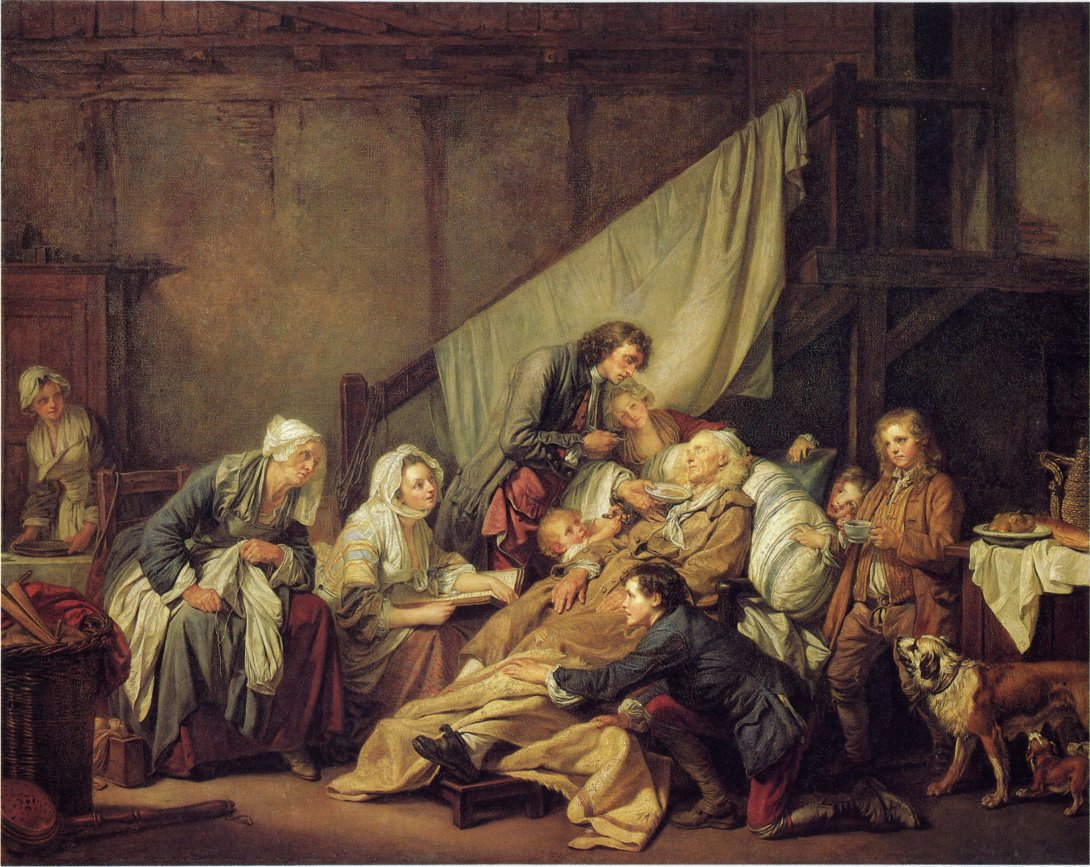
\includegraphics[angle=90, width=\linewidth]{img/GREUZE-Paralytique.jpg}
\caption{Jean-Baptiste \textsc{Greuze}, \textit{La Piété filiale} ou \textit{Le Paralytique}, 1761, Peinture sur toile, 115×146~cm, Musée de l'Ermitage, Saint-Pétersbourg.}
\end{figure}

\sujetn{%
	nomauteur=Diderot,
	prenomauteur=Denis,
	initialeprenom =D,
	particule=,
	titre = {Salon de 1763},
	semestre = \RS,
	lieu ={Amérique du Sud},
	annee =2022,
	type =,
	jour =2,
	datepub = 1763,
	ajoutref ={«~Greuze~»},
	genre =\articlel,
	corrige =,
	liencorrige={amsud_2022_2_1},
	typequn=\litt,
	typeqdeux = \phil,
	qun = {Par quelles dimensions de l'œuvre Diderot est-il touché~?},
	qdeux ={L'art ne s'adresse-t-il qu'à la sensibilité~?},
	themeprogrammequn=EXS,
	themeprogrammeqdeux=EXS}
{\chapeau{Après avoir visité une exposition organisée par l'Académie royale de peinture et de sculpture, Denis Diderot en rend compte dans le journal \emph{Correspondance littéraire}. Il s'attarde en particulier sur un tableau de Jean Baptiste Greuze intitulé \emph{La Piété filiale} (ou \emph{Le Paralytique}).}

Le genre me plaît. C'est la peinture morale. Quoi donc, le pinceau n'a-t-il pas été assez et trop longtemps consacré à la débauche et au vice~? ne devons-nous pas être satisfaits de le voir concourir enfin avec la poésie dramatique à nous toucher, à nous instruire, à nous corriger et à nous inviter à la vertu~? Courage, mon ami Greuze~! Fais de la morale en peinture, et fais-en toujours comme cela. Lorsque tu seras au moment de quitter la vie, il n'y aura aucune de tes compositions que tu ne puisses te rappeler avec plaisir. Que n'étais-tu à côté de cette jeune fille\footnote{Il s'agit d'une jeune fille, inconnue de Diderot, venue admirer le tableau de Greuze.} qui, regardant la tête de ton \emph{Paralytique}, s'écria avec une vivacité charmante~: «~ Ah, mon Dieu, comme il me touche~; mais si je le regarde encore, je crois que je vais pleurer~». Et que cette jeune fille n'était-elle la mienne~! Je l'aurais reconnue à ce mouvement. Lorsque je vis ce vieillard éloquent et pathétique, je sentis, comme elle, mon âme s'attendrir et des pleurs prêts à tomber de mes yeux.
Le tableau de la \emph{Piété filiale}\footnote{\emph{La Piété filiale} et \emph{Le Paralytique} désignent une seule et même œuvre.} a quatre pieds six pouces de large, sur trois pieds\footnote{Soit 137~cm environ de large sur~91 cm environ de haut.} de haut.

Le principal personnage, celui qui occupe le milieu de la scène, et qui fixe l'attention, est un vieillard paralytique, étendu dans son fauteuil, la tête appuyée sur un traversin, et les pieds sur un tabouret. Il est habillé. Ses jambes malades sont enveloppées d'une couverture. Il est entouré de ses enfants et de ses petits-enfants, la plupart empressés à le servir. Sa belle tête est d'un caractère si touchant~; il paraît si sensible aux services qu'on lui rend~; il a tant de peine à parler, sa voix est si faible, ses regards si tendres, son teint si pâle, qu'il faut être sans entrailles pour ne pas les sentir remuer.
\theme{peinture}\theme{art}\theme{vertu}\theme{sensibilité}\theme{morale}\theme{vie (et mort)}\theme{larmes}\theme{enfant}\theme{vieillesse}\theme{vie (et mort)!âge de la vie}\theme{famille}\theme{pitié}}

%%%%%%%%%%%%%%%%%%%%%%%%%%%%Nv-Sujet%%%%%%%%%%%%%%%%%%%%%%%%%%%%%%%%%%%%%%%%%%
\sujetn{%
	nomauteur=Giono,
	prenomauteur=Jean,
	initialeprenom =J,
	particule=,
	titre = {L'Homme qui plantait des arbres},
	semestre = \RS,
	lieu ={Amérique du Sud},
	annee =2022,
	type =,
	jour =2,
	datepub = 1953,
	ajoutref =,
	genre =\romanl,
	corrige =,
	liencorrige={amsud_2022_2_2},
	typequn=\litt,
	typeqdeux = \phil,
	qun = {Comment Giono met-il en valeur la renaissance de la région dans cet extrait~?},
	qdeux ={La nature est-elle autre chose qu'une création humaine~?},
	themeprogrammequn=EXS,
	themeprogrammeqdeux=EXS}
{\chapeau{Ce récit raconte la rencontre entre le narrateur, jeune homme d'une vingtaine d'années, et un berger solitaire, Elzéard Bouffier, retiré dans des terres désolées et arides des Alpes de Haute Provence. Une de ses seules activités est de planter des arbres sur les terres qui l'entourent.}

J'avais vu mourir trop de monde pendant cinq ans\footnote{Allusion aux années de la Première Guerre mondiale, qui ont séparé les deux hommes.} pour ne pas imaginer facilement la mort d'Elzéard Bouffier, d'autant que, lorsqu'on en a vingt, on considère les hommes de cinquante comme des vieillards à qui il ne reste plus qu'à mourir. Il n'était pas mort. Il était même fort vert. Il avait changé de métier. Il ne possédait plus que quatre brebis mais, par contre, une centaine de ruches. Il s'était débarrassé des moutons qui mettaient en péril ses plantations d'arbres. Car, me dit-il (et je le constatais), il ne s'était pas du tout soucié de la guerre. Il avait imperturbablement continué à planter.

Les chênes de 1910 avaient alors dix ans et étaient plus hauts que moi et que lui. Le spectacle était impressionnant. J'étais littéralement privé de parole et, comme lui ne parlait pas, nous passâmes tout le jour en silence à nous promener dans sa forêt. Elle avait, en trois tronçons, onze kilomètres de long et trois kilomètres dans sa plus grande largeur. Quand on se souvenait que tout était sorti des mains et de l'âme de cet homme — sans moyens techniques — on comprenait que les hommes pourraient être aussi efficaces que Dieu dans d'autres domaines que la destruction.

Il avait suivi son idée, et les hêtres qui m'arrivaient aux épaules, répandus à perte de vue, en témoignaient. Les chênes étaient drus et avaient dépassé l'âge où ils étaient à la merci des rongeurs~; quant aux desseins de la Providence\footnote{Puissance supérieure qui gouverne le monde.} elle-même, pour détruire l'œuvre créée, il lui faudrait avoir désormais recours aux cyclones. Il me montra d'admirables bosquets de bouleaux qui dataient de cinq ans, c'est-à-dire de 1915, de l'époque où je combattais à Verdun. Il leur avait fait occuper tous les fonds où il soupçonnait, avec juste raison, qu'il y avait de l'humidité presque à fleur de terre. Ils étaient tendres comme des adolescents et très décidés.

La création avait l'air, d'ailleurs, de s'opérer en chaînes. Il ne s'en souciait pas~; il poursuivait obstinément sa tâche, très simple. Mais en redescendant par le village, je vis couler de l'eau dans des ruisseaux qui, de mémoire d'homme, avaient toujours été à sec. C'était la plus formidable opération de réaction qu'il m'ait été donné de voir. Ces ruisseaux secs avaient jadis porté de l'eau, dans des temps très anciens. Certains de ces villages tristes dont j'ai parlé au début de mon récit s'étaient construits sur les emplacements d'anciens villages gallo-romains dont il restait encore des traces, dans lesquelles les archéologues avaient fouillé et ils avaient trouvé des hameçons à des endroits où au vingtième siècle, on était obligé d'avoir recours à des citernes pour avoir un peu d'eau.

Le vent aussi dispersait certaines graines. En même temps 
que l'eau réapparut réapparaissaient les saules, les osiers, les prés, les jardins, les fleurs et une certaine raison de vivre.
\theme{nature!environnement}\theme{solitude}\theme{guerre!Première Guerre mondiale}\theme{vie (et mort)}\theme{vieillesse}\theme{lyrisme}\theme{animaux}\theme{silence}\theme{berger}\theme{technique!maîtrise technique de la nature}\theme{création!humaine}\theme{renouvellement!de la nature}}

%%%%%%%%%%%%%%%%%%%%%%%%%%%%Nv-Sujet%%%%%%%%%%%%%%%%%%%%%%%%%%%%%%%%%%%%%%%%%%
\sujetn{%
	nomauteur=Camus,
	prenomauteur=Albert,
	initialeprenom =A,
	particule=,
	titre = {Noces},
	semestre = \RS,
	lieu ={Amérique du Nord},
	annee =2022,
	type =,
	jour =1,
	datepub = 1939,
	ajoutref ={«~Noces à Tipasa~»},
	genre =\romanl,
	corrige =Oui,
	liencorrige={amnord_2022_1_1},
	typequn=\litt,
	typeqdeux = \phil,
	qun = {Comment ce texte nous fait-il entendre «~la mélodie du monde~»~?},
	qdeux ={L'art réconcilie-t-il l'homme et la nature~?},
	themeprogrammequn=EXS,
	themeprogrammeqdeux=EXSMM}
{Que d'heures passées à écraser les absinthes\footnote{Absinthes,
sauges et ravenelles sont des plantes méditerranéennes.}, à caresser
les ruines, à tenter d'accorder ma respiration aux soupirs tumultueux
du monde~! Enfoncé parmi les odeurs sauvages et les concerts
d'insectes somnolents, j'ouvre les yeux et mon cœur à la grandeur
insoutenable de ce ciel gorgé de chaleur. Ce n'est pas si facile de
devenir ce qu'on est, de retrouver sa mesure profonde.

Mais à regarder l'échine solide du Chenoua\footnote{Chenoua~: Le
Chenoua est une montagne, située dans la région de Tipasa, au nord de
l'Algérie.}, mon cœur se calmait d'une étrange certitude. J'apprenais
à respirer, je m'intégrais et je m'accomplissais. Je gravissais l'un
après l'autre des coteaux dont chacun me réservait une récompense,
comme ce temple dont les colonnes mesurent la course du soleil et
d'où l'on voit le village entier, ses murs blancs et roses et ses
vérandas vertes.

Comme aussi cette basilique\footnote{Basilique~: monument de l'Église
catholique, dévoué à un saint.} sur la colline Est~: elle a gardé ses
murs et dans un grand rayon autour d'elle s'alignent des sarcophages
exhumés, pour la plupart à peine issus de la terre dont ils
participent encore. Ils ont contenu des morts~; pour le moment il y
pousse des sauges et des ravenelles.

La basilique Sainte-Salsa est chrétienne, mais à chaque fois qu'on
regarde par une ouverture, c'est la mélodie du monde qui parvient
jusqu'à nous~: coteaux plantés de pins et de cyprès, ou bien la mer
qui roule ses chiens blancs à une vingtaine de mètres. La colline qui
supporte Sainte-Salsa est plate à son sommet et le vent souffle plus
largement à travers les portiques. Sous le soleil du matin, un grand
bonheur se balance dans l'espace.
\theme{introspection!se trouver}\theme{paysage}\theme{nature!environnement}\theme{solitude}\theme{musique}}

%%%%%%%%%%%%%%%%%%%%%%%%%%%%Nv-Sujet%%%%%%%%%%%%%%%%%%%%%%%%%%%%%%%%%%%%%%%%%%
\sujetn{%
	nomauteur=Musset,
	prenomauteur=Alfred,
	initialeprenom =A,
	particule=de,
	titre = {La Nuit d'Août},
	semestre = \RS,
	lieu ={Amérique du Nord},
	annee =2022,
	type =,
	jour =2,
	datepub =1837,
	ajoutref =,
	genre =\poesie,
	corrige =Oui,
	liencorrige={amnord_2022_2_1},
	typequn=\litt,
	typeqdeux = \phil,
	qun = {En quoi le poète fait-il de la nature le reflet de sa sensibilité~?},
	qdeux ={L'art peut-il sublimer la souffrance~?},
	themeprogrammequn=EXS,
	themeprogrammeqdeux=EXS}
{\vspace*{-30pt}\par\chapeau{Dans ce poème \emph{«~La Nuit d'Août~»}, Musset présente le
dialogue entre deux personnages~: la Muse et le Poète. À la Muse qui
évoque le désenchantement de l'expérience et la déchéance de la
vieillesse, le Poète répond par ces strophes qui terminent le poème.}

\setlength{\parskip}{0pt}

Puisque l'oiseau des bois voltige et chante encore

Sur la branche où ses œufs sont brisés dans le nid~;

Puisque la fleur des champs entr'ouverte à l'aurore,

Voyant sur la pelouse une autre fleur éclore,

S'incline sans murmure et tombe avec la nuit,

Puisqu'au fond des forêts, sous les toits de verdure,

On entend le bois mort craquer dans le sentier,

Et puisqu'en traversant l'immortelle nature,

L'homme n'a su trouver de science qui dure,

Que de marcher toujours et toujours oublier~;

Puisque, jusqu'aux rochers tout se change en poussière~;

Puisque tout meurt ce soir pour revivre demain~;

Puisque c'est un engrais que le meurtre et la guerre~;

Puisque sur une tombe on voit sortir de terre

Le brin d'herbe sacré qui nous donne le pain~;

Ô Muse~! que m'importe ou la mort ou la vie~?

J'aime, et je veux pâlir~; j'aime et je veux souffrir~;

J'aime, et pour un baiser je donne mon génie~;

J'aime, et je veux sentir sur ma joue amaigrie

Ruisseler une source impossible à tarir.

J'aime, et je veux chanter la joie et la paresse,

Ma folle expérience et mes soucis d'un jour,

Et je veux raconter et répéter sans cesse

Qu'après avoir juré de vivre sans maîtresse,

J'ai fait serment de vivre et de mourir d'amour.

Dépouille devant tous l'orgueil qui te dévore,

Cœur gonflé d'amertume et qui t'es cru fermé.

Aime, et tu renaîtras~; fais-toi fleur pour éclore.

Après avoir souffert, il faut souffrir encore~;

Il faut aimer sans cesse, après avoir aimé.

\setlength{\parskip}{6pt}
\theme{nature!environnement}\theme{paysage}\theme{amour}\theme{inspiration}\theme{vie (et mort)}\theme{souffrance}\theme{nuit}}


%%%%%%%%%%%%%%%%%%%%%%%%%%%%Nv-Sujet%%%%%%%%%%%%%%%%%%%%%%%%%%%%%%%%%%%%%%%%%%
\sujetn{%
	nomauteur=Hegel,
	prenomauteur={Georg Wilhelm Friedrich},
	initialeprenom =G.~W.~F,
	particule=,
	titre = {Esthétique},
	semestre = \RS,
	lieu =Asie,
	annee =2022,
	type =,
	jour =1,
	datepub ={1818-1829},
	ajoutref ={traduction S.~\textsc{Jankélévitch}},
	genre =\essaip,
	corrige =,
	liencorrige={asi_2022_1_2},
	typequn = \phil,
	typeqdeux = \litt,
	qun = {Selon ce texte, comment la représentation artistique de nos passions permet-elle de nous en libérer~?},
	qdeux ={La littérature et les arts ont-ils vraiment un pouvoir consolateur~?},
	themeprogrammequn=EXS,
	themeprogrammeqdeux=EXS}
{Un désir est d'autant plus sauvage qu'il s'empare à lui seul de
l'homme tout entier et que l'homme n'a pas encore appris à se
différencier, en tant que généralité, par rapport à cette
détermination. Quand je dis~: ma passion est plus forte que moi, je
fais bien une différence entre mon moi abstrait et la passion~; mais
c'est là une distinction purement formelle qui signifie que je ne
suis rien en comparaison de la passion. La sauvagerie de la passion
résulte donc de l'unité qui existe entre mon moi général et la
limitation à laquelle il est soumis, de sorte que je ne connais pas
d'autre volonté que cette volonté limitée. On appelle \textit{un homme
entier}\footnote{«~un homme entier~»~: en français dans le texte.} un
homme qui concentre toute sa volonté sur une fin particulière.

C'est là la sauvagerie, force et puissance de l'homme dominé par les
passions. Elle peut être adoucie par l'art, dans la mesure où
celui-ci représente à l'homme les passions elles-mêmes, les instincts
et, en général, l'homme tel qu'il est. Et en se bornant à dérouler le
tableau des passions, l'art, alors même qu'il les flatte, le fait
pour montrer à l'homme ce qu'il est, pour l'en rendre conscient.
C'est déjà en cela que consiste son action adoucissante, car il met
ainsi l'homme en présence de ses instincts, comme s'ils étaient en
dehors de lui, et lui confère de ce fait une certaine liberté à leur
égard. Sous ce rapport, on peut dire de l'art qu'il est un
libérateur. Les passions perdent leur force, du fait même qu'elles
sont devenues objets de représentations, objets tout court.
L'objectivation\footnote{«~objectivation~»~: passage d'un vécu
intérieur à une réalité extérieure.} des sentiments a justement pour
effet de leur enlever leur intensité et de nous les rendre
extérieurs, plus ou moins étrangers. Par son passage dans la
représentation, le sentiment sort de l'état de concentration dans
lequel il se trouvait en nous et s'offre à notre libre jugement. Il
en est des passions comme de la douleur~: le premier moyen que la
nature met à notre disposition pour obtenir un soulagement d'une
douleur qui nous accable, sont les larmes~; pleurer, c'est déjà être
consolé. Le soulagement s'accentue ensuite au cours de conversations
avec des amis, et le besoin d'être soulagé et consolé peut nous
pousser jusqu'à composer des poésies. C'est ainsi que dès qu'un homme
qui se trouve plongé dans la douleur et absorbé par elle est à même
d'extérioriser cette douleur, il s'en sent soulagé, et ce qui soulage
encore davantage, c'est son expression en paroles, en chants, en sons
et en figures. Ce dernier moyen est encore plus efficace.
\theme{désir}\theme{identité!et différences}\theme{passion}\theme{moi!moi abstrait}\theme{art}\theme{liberté}\theme{émotions!objectivation des émotions}\theme{souffrance}\theme{consolation}\theme{sentiments}\theme{larmes}}

%%%%%%%%%%%%%%%%%%%%%%%%%%%%Nv-Sujet%%%%%%%%%%%%%%%%%%%%%%%%%%%%%%%%%%%%%%%%%%

\sujetn{%
	nomauteur=Dumas,
	prenomauteur=Alexandre,
	initialeprenom =A,
	particule=,
	titre = {Kean},
	semestre = \RS,
	lieu =Asie,
	annee =2022,
	type =,
	jour =2,
	datepub = 1836,
	ajoutref ={acte II, scène 4},
	genre =\theatre,
	corrige =,
	liencorrige={asi_2022_2_1},
	typequn=\litt,
	typeqdeux = \phil,
	qun = {Comment la personnalité de Kean est-elle liée à son métier d'acteur~?},
	qdeux ={Jouer un rôle, est-ce trahir son identité~?},
	themeprogrammequn=EXSMM,
	themeprogrammeqdeux=MM}
{\chapeau{
Dans cette scène, Kean, un célèbre acteur, conseille la jeune Anna qui
souhaite devenir comédienne.}

\vspace*{-18pt}\personnage{KEAN.}

Oui, je suis roi, c'est vrai… trois fois par semaine à peu près, roi
avec un sceptre de bois doré, des diamants de strass et une couronne
de carton~; j'ai un royaume de trente-cinq pieds carrés, et une
royauté qu'un bon petit coup de sifflet fait évanouir. Oh~! oui, oui,
je suis un roi bien respecté, bien puissant, et surtout bien heureux,
allez~!

\personnage{ANNA.}

Ainsi, lorsque tout le monde vous applaudit, vous envie, vous admire…

\personnage{KEAN.}

Eh bien~! parfois, je blasphème, je maudis, je jalouse le sort du
portefaix\footnote{“portefaix”~: celui dont le métier consiste à
porter des fardeaux}, courbé sous son fardeau… du laboureur sur sa
charrue, et du marin couché sur le pont du vaisseau.

\personnage{ANNA.}

Et si une femme, jeune, riche, et qui vous aimât, venait vous dire~:
Kean, ma fortune, mon amour, sont à vous… sortez de cet enfer qui
vous brûle… de cette existence qui vous dévore… quittez le théâtre…

\personnage{KEAN.}

Moi~! moi~! quitter le théâtre… moi~! Oh~! vous ne savez donc pas ce
que c'est que cette robe de Nessus\footnote{“robe de Nessus”~:
tunique empoisonnée reçue en cadeau par Hercule et qui lui brûle la
peau} qu'on ne peut arracher de dessus ses épaules qu'en déchirant sa
propre chair~: moi, quitter le théâtre, renoncer à ses émotions, à
ses éblouissements, à ses douleurs~! moi, céder la place à Kemble et
à Macready\footnote{“à Kemble et à Macready”~: acteurs rivaux de
Kean}, pour qu'on m'oublie au bout d'un an, au bout de six mois,
peut-être~! Mais rappelez-vous donc que l'acteur ne laisse rien après
lui, qu'il ne vit que pendant sa vie, que sa mémoire s'en va avec la
génération à laquelle il appartient, et qu'il tombe du jour dans la
nuit… du trône dans le néant… Non~! non~! lorsqu'on a mis le pied une
fois dans cette fatale carrière, il faut la parcourir jusqu'au bout…,
épuiser ses joies et ses douleurs, vider sa coupe et son
calice\footnote{“calice”~: vase sacré}, boire son miel et sa
lie\footnote{“lie”~: dépôt amer du vin}… Il faut finir comme on a
commencé, mourir comme on a vécu… mourir comme est mort Molière, au
bruit des applaudissements, des sifflets et des bravos~!… Mais
lorsqu'il est encore temps de ne pas prendre cette route, lorsqu'on
n'a pas franchi la barrière… il n'y faut pas… croyez-moi,
\textit{miss}, sur mon honneur~! croyez-moi.
\theme{théâtre}\theme{souvenir}\theme{identité!sociale}\theme{mensonge}\theme{rôle!jouer un rôle}\theme{mémoire}}

%%%%%%%%%%%%%%%%%%%%%%%%%%%%Nv-Sujet%%%%%%%%%%%%%%%%%%%%%%%%%%%%%%%%%%%%%%%%%%
\sujetn{%
	nomauteur=Proust,
	prenomauteur=Marcel,
	initialeprenom =M,
	particule=,
	titre = {Du côté de chez Swann},
	semestre = \RS,
	lieu ={Centres étrangers},
	annee =2022,
	type =,
	jour =1,
	datepub =1913,
	ajoutref =,
	genre =\romanl,
	corrige =Oui,
	liencorrige={cea_2022_1_2},
	typequn=\litt,
	typeqdeux = \phil,
	qun = {En quoi l'identité du personnage de Swann se métamorphose-t-elle~?},
	qdeux ={Notre personnalité sociale n'est-elle qu'une création de la pensée des autres~?},
	themeprogrammequn=MM,
	themeprogrammeqdeux=MM}
{Mais même au point de vue des plus insignifiantes choses de la vie,
nous ne sommes pas un tout matériellement constitué, identique pour
tout le monde et dont chacun n'a qu'à aller prendre connaissance
comme d'un cahier des charges ou d'un testament~; notre personnalité
sociale est une création de la pensée des autres. Même l'acte si
simple que nous appelons «~voir une personne que nous connaissons~»
est en partie un acte intellectuel. Nous remplissons l'apparence
physique de l'être que nous voyons de toutes les notions que nous
avons sur lui, et dans l'aspect total que nous nous représentons, ces
notions ont certainement la plus grande part. Elles finissent par
gonfler si parfaitement les joues, par suivre en une adhérence si
exacte la ligne du nez, elles se mêlent si bien de nuancer la
sonorité de la voix comme si celle-ci n'était qu'une transparente
enveloppe, que chaque fois que nous voyons ce visage et que nous
entendons cette voix, ce sont ces notions que nous retrouvons, que
nous écoutons. Sans doute, dans le Swann qu'ils s'étaient constitué,
mes parents avaient omis par ignorance de faire entrer une foule de
particularités de sa vie mondaine qui étaient cause que d'autres
personnes, quand elles étaient en sa présence, voyaient les élégances
régner dans son visage et s'arrêter à son nez busqué comme à leur
frontière naturelle~; mais aussi ils avaient pu entasser dans ce
visage désaffecté de son prestige, vacant et spacieux, au fond de ces
yeux dépréciés, le vague et doux résidu – mi-mémoire, mi-oubli – des
heures oisives passées ensemble après nos dîners hebdomadaires,
autour de la table de jeu ou au jardin, durant notre vie de bon
voisinage campagnard. L'enveloppe corporelle de notre ami en avait
été si bien bourrée, ainsi que de quelques souvenirs relatifs à ses
parents, que ce Swann-là était devenu un être complet et vivant, et
que j'ai l'impression de quitter une personne pour aller vers une
autre qui en est distincte, quand, dans ma mémoire, du Swann que j'ai
connu plus tard avec exactitude, je passe à ce premier Swann – à ce
premier Swann dans lequel je retrouve les erreurs charmantes de ma
jeunesse et qui d'ailleurs ressemble moins à l'autre qu'aux personnes
que j'ai connues à la même époque, comme s'il en était de notre vie
ainsi que d'un musée où tous les portraits d'un même temps ont un air
de famille, une même tonalité – à ce premier Swann rempli de loisir,
parfumé par l'odeur du grand marronnier, des paniers de framboises et
d'un brin d'estragon.
\theme{identité!sociale}\theme{moi!fragmentation du moi}\theme{autrui}\theme{reconnaissance}\theme{corps}\theme{identité!et changements}\theme{mémoire}\theme{oubli}}

%%%%%%%%%%%%%%%%%%%%%%%%%%%%Nv-Sujet%%%%%%%%%%%%%%%%%%%%%%%%%%%%%%%%%%%%%%%%%%

\sujetn{%
	nomauteur=Chateaubriand,
	prenomauteur={François-René},
	initialeprenom ={F.-R},
	particule=de,
	titre = {Mémoires d'outre-tombe},
	semestre = \RS,
	lieu = {Centres étrangers},
	annee =2022,
	type =,
	jour =2,
	datepub ={1809-1841},
	ajoutref = {livre troisième, chapitre IV},
	genre =\memoire,
	corrige =Oui,
	liencorrige={cea_2022_2_1},
	typequn=\litt,
	typeqdeux = \phil,
	qun = {Comment l'auteur s'approprie-t-il une expérience de l'enfance~?},
	qdeux ={La sensibilité est-elle formée par les seules épreuves de la vie~?},
	themeprogrammequn=MM,
	themeprogrammeqdeux=EXSMM}
{Quelques martinets, qui durant l'été s'enfonçaient en criant dans les
trous des murs, étaient mes seuls compagnons. La nuit, je
n'apercevais qu'un petit morceau de ciel et quelques étoiles. Lorsque
la lune brillait et qu'elle s'abaissait à l'occident, j'en étais
averti par ses rayons, qui venaient à mon lit au travers des carreaux
losangés de la fenêtre. Des chouettes, voletant d'une tour à l'autre,
passant et repassant entre la lune et moi, dessinaient sur mes
rideaux l'ombre mobile de leurs ailes. Relégué dans l'endroit le plus
désert, à l'ouverture des galeries, je ne perdais pas un murmure des
ténèbres. Quelquefois le vent semblait courir à pas légers~;
quelquefois il laissait échapper des plaintes~; tout à coup ma porte
était ébranlée avec violence, les souterrains poussaient des
mugissements, puis ces bruits expiraient pour recommencer encore. À
quatre heures du matin, la voix du maître du château, appelant le
valet de chambre à l'entrée des voûtes séculaires, se faisait
entendre comme la voix du dernier fantôme de la nuit. Cette voix
remplaçait pour moi la douce harmonie au son de laquelle le père de
Montaigne éveillait son fils.

L'entêtement du comte de Chateaubriand à faire coucher un enfant seul
au haut d'une tour pouvait avoir quelque inconvénient~; mais il
tourna à mon avantage. Cette manière violente de me traiter me laissa
le courage d'un homme, sans m'ôter cette sensibilité d'imagination
dont on voudrait aujourd'hui priver la jeunesse. Au lieu de chercher
à me convaincre qu'il n'y avait point de revenants, on me força de
les braver. Lorsque mon père me disait, avec un sourire ironique~:
«~Monsieur le chevalier aurait-il peur~?~» il m'eût fait coucher avec
un mort. Lorsque mon excellente mère me disait~: «~Mon enfant, tout
n'arrive que par la permission de Dieu~; vous n'avez rien à craindre
des mauvais esprits, tant que vous serez bon chrétien~;~» j'étais
mieux rassuré que par tous les arguments de la philosophie. Mon
succès fut si complet que les vents de la nuit, dans ma tour
déshabitée, ne servaient que de jouets à mes caprices et d'ailes à
mes songes. Mon imagination allumée, se propageant sur tous les
objets, ne trouvait nulle part assez de nourriture et aurait dévoré
la terre et le ciel.
\theme{nature!environnement}\theme{paysage}\theme{solitude}\theme{nuit}\theme{imagination}\theme{enfant}\theme{sensibilité}\theme{vie (et mort)!âge de la vie}}

%%%%%%%%%%%%%%%%%%%%%%%%%%%%Nv-Sujet%%%%%%%%%%%%%%%%%%%%%%%%%%%%%%%%%%%%%%%%%%

\sujetn{%
	nomauteur=Verlaine,
	prenomauteur=Paul,
	initialeprenom =P,
	particule=,
	titre = {Fêtes galantes},
	semestre = \RS,
	lieu =Liban,
	annee =2022,
	type =,
	jour =1,
	datepub =1869,
	ajoutref =,
	genre =\poesie,
	corrige =,
	liencorrige={lib2022_1_1},
	typequn=\litt,
	typeqdeux = \phil,
	qun = {Quelle image ce poème donne-t-il de la relation amoureuse~?},
	qdeux ={Nos sentiments résistent-ils au temps~?},
	themeprogrammequn=EXS,
	themeprogrammeqdeux=EXSMM}
{\begin{center}COLLOQUE SENTIMENTAL\end{center}

\setlength{\parskip}{0pt}

\bigskip

Dans le vieux parc solitaire et glacé

Deux formes ont tout à l'heure passé.

\medskip

Leurs yeux sont morts et leurs lèvres sont molles,

Et l'on entend à peine leurs paroles.

\medskip

Dans le vieux parc solitaire et glacé

Deux spectres ont évoqué le passé.

\medskip

—~Te souvient-il de notre extase ancienne~?

—~Pourquoi voulez-vous donc qu'il m'en souvienne~?

\medskip

—~Ton cœur bat-il toujours à mon seul nom~?

Toujours vois-tu mon âme en rêve~? – Non.

\medskip

—~Ah~! les beaux jours de bonheur indicible

Où nous joignions nos bouches~! – C'est possible.

\medskip

—~Qu'il était bleu, le ciel, et grand, l'espoir~!

—~L'espoir a fui, vaincu, vers le ciel noir.

\medskip

Tels ils marchaient dans les avoines folles,

Et la nuit seule entendit leurs paroles.

\setlength{\parskip}{6pt}
\theme{amour}\theme{souvenir}\theme{oubli}\theme{nuit}\theme{solitude}\theme{sentiments}}

%%%%%%%%%%%%%%%%%%%%%%%%%%%%Nv-Sujet%%%%%%%%%%%%%%%%%%%%%%%%%%%%%%%%%%%%%%%%%%

\sujetn{%
	nomauteur=Noailles,
	prenomauteur={Anna},
	initialeprenom={A},
	particule=de,
	titre = {Le visage émerveillé},
	semestre = \RS,
	lieu =Liban,
	annee =2022,
	type =,
	jour =2,
	datepub =1904,
	ajoutref =,
	genre =\romanl,
	corrige =,
	liencorrige={lib2022_2_1},
	typequn=\litt,
	typeqdeux = \phil,
	qun = {Peut-on dire que le personnage de Sophie est dominé par sa sensibilité~?},
	qdeux ={Nos choix de vie peuvent-ils se faire contre nos sentiments~?},
	themeprogrammequn=EXS,
	themeprogrammeqdeux=EXS}
{\chapeau{
La sœur Sainte-Sophie vit dans un couvent depuis deux ans, parce
qu'elle «~aime Dieu, la mère abbesse, le silence~». Un jeune homme,
Julien, vient admirer un tableau dans la chapelle du couvent. C'est
le coup de foudre mais, au nom de sa foi, Sophie décide de renoncer à
Julien.}

{\raggedleft
10 décembre.
\par}

Mon chéri, voilà plus de trois semaines que je suis malade. On ne me
donne pas vos lettres, et si je vous écrivais, on ne vous ferait pas
parvenir les miennes.

Je n'ai plus de force, je voudrais beaucoup mourir. Par moments, je
vous vois comme si vous étiez très loin, je n'entends presque plus
votre voix, et à d'autres instants votre image emplit et déchire mon
cœur resserré. Je ne sais si je redoute ou si je souhaite que vous
vous effaciez en moi.

Tout ce qu'on peut souffrir, je l'ai souffert~: j'ai pensé m'éteindre
de violence et de colère, et maintenant je souffre d'une douce et
terrible sentimentalité~; ce sentiment fait plus mal que les autres~;
je pense à vous avec une tendresse qui me tue. Je suis là, couchée,
près de la sœur Marthe qui brode. Je vois par la fenêtre un ciel
d'hiver très bleu.

Si je n'avais connu que votre passion et la mienne, je pourrais,
aujourd'hui où je suis si malade, oublier, mais j'ai connu, mon
chéri, votre bonté.

J'ai connu votre bonté pour moi auprès de laquelle l'affection de la
supérieure est pauvre et blessante, la sympathie de mes sœurs
misérable.

Vous m'avez tant donné, dans des moments de douceur sans limite, que
l'attention moindre de toutes les autres âmes ne peut plus que
m'offenser. La pureté, l'amitié infinie, c'est nous qui les avons
goûtées, dans les instants où, sans secret, sans défiance, nous fûmes
vraiment des âmes mêlées, des regards pareils. Que les amies
parfaites aient entre elles besoin de précautions et d'égards, que
les frères et les parents se respectent et craignent de s'offenser,
mais nous, quels soins eussions-nous pu prendre d'une âme qui nous
était commune~?

Je me souviens que vous sembliez oppressé la nuit où vous m'avez
quittée.

Hélas~! je n'ai pas suivi votre douleur. Comment étiez-vous quand vous
êtes rentré dans votre chambre, quand vos bras pendaient le long de
votre corps, quand vous vous êtes assis avec stupeur, car les hommes,
n'est-ce pas, sont étonnés de souffrir~? Mon chéri, cette
sentimentalité dont la douceur fait mal, je ne puis l'écarter de moi,
elle pèse sur mon cœur et m'étouffe, comme ces beaux chats chauds et
fourrés qui s'endorment la nuit sur la poitrine des petits enfants.
\theme{amour}\theme{vie (et mort)}\theme{émotions}\theme{passion}\theme{sentiments}\theme{souffrance}\theme{religion}\theme{sensibilité}\theme{maladie}}

%%%%%%%%%%%%%%%%%%%%%%%%%%%%Nv-Sujet%%%%%%%%%%%%%%%%%%%%%%%%%%%%%%%%%%%%%%%%%%

\sujetn{%
	nomauteur=Albert-Birot,
	prenomauteur=Pierre,
	initialeprenom ={P},
	titre = {Poésies},
	semestre = \RS,
	lieu =Métropole,
	annee =2022,
	type =,
	jour =1,
	datepub =1926,
	ajoutref =«~L'affaire Narcisse~»,
	genre =\poesie,
	corrige =Oui,
	liencorrige={met_2022_1_1},
	typequn=\litt,
	typeqdeux = \phil,
	qun = {«~L'affaire Narcisse~»~: comment votre lecture du poème éclaire-t-elle ce titre~?},
	qdeux ={Se connaître soi-même, est-ce se découvrir «~pièce unique~»~?},
	themeprogrammequn=OdS,
	themeprogrammeqdeux=MM}
{%
\begin{center}
L'AFFAIRE NARCISSE
\end{center}

\setlength{\parskip}{0pt}

\bigskip

Narcisse fils de Céphise\footnote{Personnage de la mythologie grecque, fils de la nymphe Liriope et du fleuve Céphise, Narcisse est doté d'une grande beauté. Indifférent à l'admiration qu'on lui voue, il aperçoit un jour son reflet dans l'eau et en tombe amoureux. A force d'auto-contemplation, il finit par mourir, et est métamorphosé en fleur.} n'est plus depuis des montagnes de temps

En nos âges il n'est plus de ces Narcisse-là

Seule une fleur nous reste

Et pourtant nous avons des miroirs autrement plus parfaits que la
fontaine

Où s'admira ce trop joli garçon

Ne dirai point que ne suis jamais venu devant ma glace

Au cours de mon printemps de mon été même des froides saisons qui
suivent

Mais pas une fois ne me suis dit celui-là c'est moi

Or bien hier

Sans doute disons

Glace parfaite

Lumière magnifique

Et temps à perdre

Celui-là fut moi

Je l'ai vu totalement vu

Et j'ai dû me dire et me redire tant que j'ai pu

Cet homme qui est là devant c'est toi complètement toi

De la tête aux pieds et quelle découverte moi je suis fait comme tout
homme est fait

Et pourtant ne ressemble à aucun

Toutefois ne sais si vais m'aimer autant que je m'aimais avant de me
connaître

Enfin c'est agréable tout de même de se savoir pièce unique

Et n'oublions pas que chaque être humain peut en dire autant

A bien regarder Narcisse avait raison

Un homme ça vaut la peine d'être vu

\setlength{\parskip}{6pt}
\theme{narcissisme}\theme{contemplation}\theme{reconnaissance}\theme{corps}\theme{identité}\theme{identité!comme unicité}\theme{introspection}}

%%%%%%%%%%%%%%%%%%%%%%%%%%%%Nv-Sujet%%%%%%%%%%%%%%%%%%%%%%%%%%%%%%%%%%%%%%%%%%

\sujetn{%
	nomauteur=Rousseau,
	prenomauteur=Jean-Jacques,
	initialeprenom ={J.-J},
	titre = {Lettres morales},
	semestre = \RS,
	lieu =Métropole,
	annee =2022,
	type =,
	jour =2,
	datepub =1758,
	ajoutref ={Lettre VI},
	genre =\lettrep,
	corrige =Oui,
	liencorrige={met_2022_2_1},
	typequn = \phil,
	typeqdeux = \litt,
	qun = {Dans quelle mesure pouvons-nous redevenir nous-mêmes~?},
	qdeux ={Lire permet-il d'accéder à une meilleure connaissance de soi~?},
	themeprogrammequn=MM,
	themeprogrammeqdeux=MM}
{Quand je vois chacun de nous sans cesse occupé de l'opinion publique
étendre pour ainsi dire son existence tout autour de lui sans en
réserver presque rien dans son propre cœur, je crois voir un petit
insecte former de sa substance une grande toile par laquelle seule il
paraît sensible tandis qu'on le croirait mort dans son trou. La
vanité de l'homme est la toile d'araignée qu'il tend sur tout ce qui
l'environne. L'une est aussi solide que l'autre, le moindre fil qu'on
touche met l'insecte en mouvement, il mourrait de langueur si l'on
laissait la toile tranquille, et si d'un doigt on la déchire il
achève de s'épuiser plutôt que de ne la pas refaire à l'instant.
Commençons par redevenir nous, par nous concentrer en nous, par
circonscrire notre âme des mêmes bornes que la nature a données à
notre être, commençons en un mot par nous rassembler où nous sommes,
afin qu'en cherchant à nous connaître tout ce qui nous compose vienne
à la fois se présenter à nous. Pour moi, je pense que celui qui sait
le mieux en quoi consiste le moi humain est le plus près de la
sagesse et que comme le premier trait d'un dessin se forme des lignes
qui le terminent, la première idée de l'homme est de le séparer de
tout ce qui n'est pas lui.

Mais comment se fait cette séparation~? Cet art n'est pas si difficile
qu'on pourrait croire, ou du moins la difficulté n'est pas où on la
croit, il dépend plus de la volonté que des lumières, il ne faut
point un appareil d'études et de recherches pour y parvenir. Le jour
nous éclaire, et le miroir est devant nous~; mais pour le voir il
faut jeter les yeux et le moyen de les y fixer est d'écarter les
objets qui nous en détournent. Recueillez-vous, cherchez la solitude,
voilà d'abord tout le secret et par celui-là seul on découvre bientôt
les vôtres. Pensez-vous en effet que la philosophie nous apprenne à
rentrer en nous – mêmes~? Ah combien l'orgueil sous son nom nous en
écarte~! C'est tout le contraire ma charmante amie, il faut commencer
par rentrer en soi pour apprendre à philosopher.
\theme{identité!sociale}\theme{rôle!jouer un rôle}\theme{moi!unité du moi}\theme{nature!nature humaine}\theme{soi!difficile accès à soi}\theme{solitude}\theme{philosophie}\theme{moi!frontières du moi}}

%%%%%%%%%%%%%%%%%%%%%%%%%%%%%Nv-Sujet%%%%%%%%%%%%%%%%%%%%%%%%%%%%%%%%%%%%%%%%

\sujetn{%
	nomauteur=Maupassant,
	prenomauteur={Guy},
	initialeprenom ={G},
	particule=de,
	titre = {Fort comme la mort},
	semestre = \RS,
	lieu =Métropole,
	annee =2022,
	type =Remplacement,
	jour =1,
	datepub =1889,
	ajoutref =,
	genre =\romanl,
	corrige =Oui,
	liencorrige={metrem_2022_1_2},
	typequn=\litt,
	typeqdeux = \phil,
	qun = {Que révèle ici la métamorphose physique~?},
	qdeux ={La souffrance a-t-elle un effet sur ce que je suis~?},
	themeprogrammequn=MM,
	themeprogrammeqdeux=EXSMM}
{Elle se croyait même au début d'une période heureuse et tranquille quand la mort de sa mère vint la frapper en plein cœur. Ce fut, pendant les premiers jours, un de ces désespoirs profonds qui ne laissent place à nulle autre pensée. Elle restait du matin au soir abîmée dans la désolation, cherchant à se rappeler mille choses de la morte, des paroles familières, sa figure d'autrefois, des robes qu'elle avait portées jadis, comme si elle eût amassé au fond de sa mémoire des reliques, et recueilli dans le passé disparu tous les intimes et menus souvenirs dont elle alimenterait ses cruelles rêveries. Puis quand elle fut arrivée ainsi à un tel paroxysme\footnote{«~paroxysme~»~: stade le plus élevé.} de désespoir, qu'elle avait à tout instant des crises de nerfs et des syncopes\footnote{«~syncopes~»~: pertes de connaissance.}, toute cette peine accumulée jaillit en larmes, et, jour et nuit, coula de ses yeux.

Or, un matin, comme sa femme de chambre entrait et venait d'ouvrir les volets et les rideaux en demandant~: «~Comment va Madame aujourd'hui~?~», elle répondit, se sentant épuisée et courbaturée à force d'avoir pleuré~: «~Oh, pas du tout. Vraiment, je n'en puis plus.~» La domestique qui tenait le plateau portant le thé regarda sa maîtresse, et émue de la voir si pâle dans la blancheur du lit, elle balbutia avec un accent triste et sincère~:

— En effet, Madame a très mauvaise mine. Madame ferait bien de se soigner.

Le ton dont cela fut dit enfonça au cœur de la comtesse une petite piqûre comme d'une pointe d'aiguille, et dès que la bonne fut partie, elle se leva pour aller voir sa figure dans sa grande armoire à glace.

Elle demeura stupéfaite en face d'elle-même, effrayée de ses joues creuses, de ses yeux rouges, du ravage produit sur elle par ces quelques jours de souffrance. Son visage qu'elle connaissait si bien, qu'elle avait si souvent regardé en tant de miroirs divers, dont elle savait toutes les expressions, toutes les gentillesses, tous les sourires, dont elle avait déjà bien des fois corrigé la pâleur, réparé les petites fatigues, détruit les rides légères apparues au trop grand jour, au coin des yeux, lui sembla tout à coup celui d'une autre femme, un visage nouveau qui se décomposait, irréparablement malade.

Pour se mieux voir, pour mieux constater ce mal inattendu, elle s'approcha jusqu'à toucher la glace du front, si près que son haleine, répandant une buée sur le verre, obscurcit, effaça presque l'image blême qu'elle contemplait. Elle dut alors prendre un mouchoir pour essuyer la brume de son souffle, et frissonnante d'une émotion bizarre, elle fit un long et patient examen des altérations de son visage. D'un doigt léger elle tendit la peau des joues, lissa celle du front, releva les cheveux, retourna les paupières pour regarder le blanc de l'œil. Puis elle ouvrit la bouche, inspecta ses dents un peu ternies où des points d'or brillaient, s'inquiéta des gencives livides et de la teinte jaune de la chair au-dessus des joues et sur les tempes.

Elle mettait à cette revue de la beauté défaillante tant d'attention qu'elle n'entendit pas ouvrir la porte, et qu'elle tressaillit jusqu'au cœur quand sa femme de chambre, debout derrière elle, lui dit~:

— Madame a oublié de prendre son thé.

La comtesse se retourna, confuse, surprise, honteuse, et la domestique, devinant sa pensée, reprit~:

— Madame a trop pleuré, il n'y a rien de pire que les larmes pour vider la peau. C'est le sang qui tourne en eau.
\theme{souffrance}\theme{tristesse}\theme{deuil}\theme{larmes}\theme{maladie}\theme{mémoire}\theme{souvenir}}

%%%%%%%%%%%%%%%%%%%%%%%%%%%%%Nv-Sujet%%%%%%%%%%%%%%%%%%%%%%%%%%%%%%%%%%%%%%%%%
\sujetn{%
	nomauteur=Rilke,
	prenomauteur=Rainer Maria,
	initialeprenom ={R.~M},
	particule=,
	titre = {Lettres à un jeune poète},
	semestre = \RS,
	lieu =Métropole,
	annee =2022,
	type =Remplacement,
	jour =2,
	datepub =1929,
	ajoutref ={trad. C.~\textsc{Mouchard}},
	genre =\lettrel,
	corrige =Oui,
	liencorrige={metrem_2022_2_2},
	typequn=\litt,
	typeqdeux = \phil,
	qun = {D'après ce texte, comment la tristesse nous transforme-t-elle~?},
	qdeux ={Se connaître est-ce comprendre ce que l'on ressent~?},
	themeprogrammequn=EXSMM,
	themeprogrammeqdeux=EXSMM}
{\chapeau{Rainer Maria Rilke s'adresse au «~jeune poète~» Franz Kappus.}

Vous avez eu maintes grandes tristesses, qui ont passé. Et vous dites que c'est aussi ce caractère passager qui vous a été pénible et contrariant. Mais réfléchissez, je vous prie~: ces grandes tristesses ne vous ont-elles pas plutôt centralement traversé~? Maintes choses en vous ne se sont-elles pas transformées, n'avez-vous pas changé en tel point, tel endroit de votre être, tandis que vous étiez triste~? Seules sont dangereuses et mauvaises les tristesses qu'on emporte au milieu des gens pour en couvrir la voix~; comme des maladies superficiellement et sottement traitées, elles ne font que reculer, et leur éruption, après une petite pause, est d'autant plus effroyable~; elles s'accumulent au-dedans, elles sont de la vie, de la vie non vécue, rejetée, perdue, de la vie dont on peut mourir. S'il nous était possible de voir un peu plus loin que notre savoir ne porte, et encore un peu au-delà des avant-postes de notre intuition, peut-être supporterions-nous alors nos tristesses avec plus de confiance que nos joies. Car elles sont les instants où quelque chose de nouveau est entré en nous, quelque chose d'inconnu~; nos sentiments se taisent, en une réticence craintive, tout en nous recule, il se fait un silence, et le nouveau, que personne ne connaît, se tient là, au milieu, muet.

Je crois que presque toutes nos tristesses sont des moments de tension que nous ressentons comme de la paralysie, sourds que nous sommes à la vie de nos sentiments frappés d'étrangeté. C'est que nous sommes seuls avec l'étranger qui est entré en nous~; c'est que tout le familier, tout l'habituel nous est pour un instant enlevé~; et que nous nous trouvons au milieu d'une transition où nous ne pouvons rester arrêtés. Voilà pourquoi la tristesse est passagère~: le nouveau en nous, venu s'ajouter, est entré dans notre cœur, a pénétré dans sa loge la plus intime, mais, là même, il n'est plus – est déjà dans le sang. Et nous n'avons pas connaissance de ce que c'était. On pourrait facilement nous faire croire que rien ne s'est passé~; et pourtant nous nous sommes transformés comme se transforme une maison où un hôte est entré. Nous ne pouvons dire qui est venu, nous ne le saurons peut-être jamais, mais bien des indices donnent à penser que c'est l'avenir qui, de cette manière, entre en nous, pour se transformer en nous, longtemps avant que de survenir.
\theme{tristesse}\theme{temps!éphémère}\theme{poésie}\theme{vie (et mort)}\theme{émotions}\theme{création}\theme{nouveauté}\theme{intime}\theme{avenir}\theme{inconnu}}

%%%%%%%%%%%%%%%%%%%%%%%%%%%%Nv-Sujet%%%%%%%%%%%%%%%%%%%%%%%%%%%%%%%%%%%%%%%%%%
\sujetn{%
	nomauteur=Présumey,
	prenomauteur=Pierre,
	initialeprenom =P,
	particule=,
	titre = {Tout ce qu'on peut},
	semestre = \RS,
	lieu =Nouvelle-Calédonie,
	annee =2022,
	type =,
	jour =2,
	datepub =2015,
	ajoutref =,
	genre =\poesie,
	corrige =,
	liencorrige={nca2022_2_1},
	typequn=\litt,
	typeqdeux = \phil,
	qun = {Le titre rend-il bien compte du poème~?},
	qdeux ={Jusqu'à quel point peut-on connaître la vie d'un homme~?},
	themeprogrammequn=OdS,
	themeprogrammeqdeux=MM}
{\vspace{-12pt}
\begin{center}
Tout ce qu'on peut
\end{center}
\setlength{\parskip}{0pt}

\medskip

On ne peut pas tenir entre ses mains la vie

D'un homme comme on tiendrait une valise pleine,

Comme on tiendrait un fagot de branches mortes,

Comme on tiendrait une pile de draps blancs,

Un panier de cerises, une corbeille de reines-claudes,

Comme on tiendrait dans son regard du haut

De la montagne tout un pays avec ses fleuves,

Avec ses collines désirables, avec ses plaines

Bien tracées~; on ne peut pas tenir entre

Ses mains la vie d'un homme tout entier

De sa chute dans le temps, à sa chute

Hors du temps, de son entrée dans la lumière

A sa sortie de la lumière~; on ne peut pas.

Tout ce qu'on peut c'est

Redire deux ou trois mots qu'il avait coutume

De dire au moment de se jeter dans le vent,

Manger les miettes du pain qu'il mangeait en partant,

Repasser son regard entre les rives où

Son regard passait, parce que c'était là

Que ses mains tenaient leur pays tout entier,

Comme un fagot de branches sèches,

Comme une pile de draps blancs bien repassés,

Comme un panier de cerises, c'était là que,

Tombé dans le temps, il mettait sa vie

Dans ses mains comme on remplit toute

Une corbeille de reines-claudes, cela

C'est tout ce qu'on peut pour le moment.

\begin{flushright}
(5 décembre 2012)\hspace*{3cm}
\end{flushright}

\setlength{\parskip}{6pt}
\theme{vie (et mort)}\theme{mort}\theme{temps}\theme{nature!environnement}\theme{mémoire}\theme{souvenir}\theme{lumière}\theme{naissance}\theme{vie (et mort)!fin de vie}\theme{temps!passage du temps}\theme{vie (et mort)!âge de la vie}\theme{autrui!comme inconnu}\theme{finitude}\theme{paysage}\theme{mémoire}\theme{souvenir}\theme{identité}\theme{existence}\theme{transmission}\theme{héritage}}

%%%%%%%%%%%%%%%%%%%%%%%%%%%%Nv-Sujet%%%%%%%%%%%%%%%%%%%%%%%%%%%%%%%%%%%%%%%%%%

\sujetn{%
	nomauteur=Beauvoir,
	prenomauteur=Simone,
	initialeprenom =S,
	particule =de,
	titre = {Mémoires d'une jeune fille rangée},
	semestre = \RS,
	lieu =Polynésie,
	annee =2022,
	type =,
	jour =1,
	datepub =1958,
	ajoutref =,
	genre =\autobiographie,
	corrige =,
	liencorrige={pol2022_1_1},
	typequn=\litt,
	typeqdeux = \phil,
	qun = {Pourquoi le passage de l'enfance à l'âge adulte effraie-t-il Simone de Beauvoir~?},
	qdeux ={Est-on le même à tous les âges de la vie~?},
	themeprogrammequn=MM,
	themeprogrammeqdeux=MM}
{Par les beaux jours d'été, il\footnote{Il s'agit du père de Simone de
Beauvoir} nous emmenait parfois, après le dîner, faire un tour au
Luxembourg\footnote{Le Jardin du Luxembourg qui jouxte le Sénat à
Paris.}~: nous mangions des glaces, à une terrasse de la place
Médicis, et, nous traversions à nouveau le jardin dont la sonnerie
d'un clairon annonçait la fermeture. J'enviais aux habitants du Sénat
leurs rêveries nocturnes, dans les allées désertes. La routine de mes
journées avait autant de rigueur que le rythme des saisons~: le
moindre écart me jetait dans l'extraordinaire. Marcher dans la
douceur du crépuscule, à l'heure où d'habitude maman verrouillait la
porte d'entrée, c'était aussi surprenant, aussi poétique qu'au cœur
de l'hiver une aubépine en fleur.

Il y eut un soir tout à fait insolite où nous bûmes un chocolat à la
terrasse de Prévost, face à l'immeuble du \textit{Matin}\footnote{Le
Matin, journal quotidien créé en 1883.}. Un journal lumineux
annonçait les péripéties du match qui se déroulait à New York entre
Carpentier et Dempsey\footnote{Allusion au «~combat du siècle~» entre
les champions de boxe Jack Dempsey et Georges Carpentier, le 2
juillet 1921.}. Le carrefour était noir de monde. Quand Carpentier
fut mis K.-O., il y eut des hommes et des femmes qui fondirent en
larmes~; je rentrai à la maison toute fière d'avoir assisté à ce
grand événement. Mais je n'aimais pas moins nos soirées quotidiennes
dans le bureau calfeutré~; mon père nous lisait \textit{Le Voyage de
M.~Perrichon}\footnote{Le Voyage de M. Perrichon, comédie d'Eugène
Labiche et Edouard Martin, représentée pour la première fois à Paris
en 1860.}, ou bien nous lisions, côte à côte, chacun pour soi. Je
regardais mes parents, ma sœur, et j'avais chaud au cœur. «~Nous
quatre~!~» me disais-je avec ravissement. Et je pensais~: «~Que nous
sommes heureux~!~»

Une seule chose, par instants, m'assombrissait~: un jour, je le
savais, cette période de ma vie s'achèverait. Cela ne paraissait pas
vraisemblable. Quand on a aimé ses parents pendant vingt ans, comment
peut-on, sans mourir de douleur, les quitter pour suivre un inconnu~?
et comment peut-on, alors qu'on s'est passé de lui pendant vingt ans,
se mettre à aimer du jour au lendemain un homme qui ne vous est rien
? J'interrogeai papa~: «~Un mari, c'est autre chose~», répondit-il~:
il eut un petit sourire qui ne m'éclaira pas. Je considérais toujours
avec déplaisir le mariage. Je n'y voyais pas une servitude, car maman
n'avait rien d'une opprimée~; c'était la promiscuité qui me rebutait.
«~Le soir, au lit, on ne peut même pas pleurer tranquillement si on
en a envie~!~» me disais-je avec effroi. Je ne sais pas si mon
bonheur était entrecoupé de crises de tristesse, mais souvent la nuit
je me faisais pleurer pour le plaisir~; m'obliger à réfréner mes
larmes ces larmes, c'eût été me refuser ce minimum de liberté dont
j'avais un impérieux besoin. Tout le jour, je sentais des regards
braqués sur moi~; j'aimais mon entourage, mais quand je me couchais
le soir, j'éprouvais un vif soulagement à l'idée de vivre enfin
quelques instants sans témoin~; alors, je pouvais m'interroger, me
souvenir, m'émouvoir, prêter l'oreille à ces rumeurs timides que la
présence des adultes étouffe. Il m'eût été odieux qu'on me privât de
ce répit. Il me fallait échapper au moins quelques instants à toute
sollicitude et me parler en paix sans que personne m'interrompît.
\theme{habitude}\theme{histoire}\theme{temps!éphémère}\theme{enfant}\theme{bonheur}\theme{solitude}\theme{vie (et mort)!âge de la vie}\theme{larmes}\theme{famille}\theme{émotions}\theme{mariage}}

%%%%%%%%%%%%%%%%%%%%%%%%%%%%Nv-Sujet%%%%%%%%%%%%%%%%%%%%%%%%%%%%%%%%%%%%%%%%%%

\sujetn{%
	nomauteur=Freud,
	prenomauteur=Sigmund,
	initialeprenom =S,
	particule=,
	titre = {Le malaise dans la culture},
	semestre = \RS,
	lieu =Polynésie,
	annee =2022,
	type =,
	jour =2,
	datepub =1929,
	ajoutref ={trad. Dorian \textsc{Astor}},
	genre =\essaip,
	corrige =,
	liencorrige={pol2022_2_2},
	typequn = \phil,
	typeqdeux = \litt,
	qun = {Qu'est-ce qui explique selon Freud les fluctuations du moi~?},
	qdeux ={Se raconter, est-ce explorer les «~frontières du moi~»~?},
	themeprogrammequn=MM,
	themeprogrammeqdeux=MM}
{La pathologie nous fait connaître un grand nombre d'états dans
lesquels la démarcation du moi d'avec le monde qui l'entoure devient
incertaine, ou dans lesquels les frontières sont tracées de manière
vraiment incorrecte~; des cas où des parties de notre propre corps,
et même des pans de vie de notre âme, perceptions, pensées,
sentiments, apparaissent comme étrangers et n'appartenant pas au moi,
d'autres où l'on impute au monde extérieur ce qui est manifestement
né dans le moi et devrait être reconnu par lui. Ainsi, le sentiment
du moi est soumis lui aussi à des perturbations, et les frontières du
moi ne sont pas constantes.

Une autre réflexion consiste à dire~: ce sentiment du moi de l'adulte
ne peut avoir été tel dès le début. Il doit avoir suivi un
développement qu'on ne peut évidemment pas démontrer, mais qu'on peut
reconstruire avec une certaine vraisemblance. Le nourrisson n'isole
pas encore son moi d'un monde extérieur qui est la source des
sensations affluant sur lui. Il apprend à le faire peu à peu par
diverses excitations. Cela doit lui faire la plus forte impression,
que certaines sources d'excitations, dans lesquelles il reconnaîtra
plus tard ses organes corporels, puissent à tout moment lui faire
parvenir des sensations, tandis que d'autres se dérobent à lui par
moments – parmi elles, celle qu'il désire le plus~: le sein maternel
–, qu'il ne peut rappeler qu'en les réclamant par des cris. Par là,
un «~objet~» s'oppose d'abord au moi, comme quelque chose qui se
trouve «~à l'extérieur~», et qui ne peut apparaître que sous la
contrainte d'une action particulière. Une autre impulsion, au
détachement du moi d'avec la masse des sensations, donc à la
reconnaissance d'un «~dehors~», d'un monde extérieur, est donnée par
les fréquentes, diverses et inévitables sensations de douleur et de
déplaisir que le tout-puissant principe de plaisir\footnote{Le
principe de plaisir désigne la tendance des pulsions inconscientes à
rechercher le plaisir, quitte à s'écarter de la réalité.} commande de
suspendre et d'éviter. Une tendance se crée à isoler du moi ce qui
peut devenir source d'un tel déplaisir, à le rejeter à l'extérieur, à
former un pur moi hédonique\footnote{Hédonique~: qui renvoie au
principe de plaisir.}, auquel s'oppose un dehors étranger et
menaçant.
\theme{moi!frontières du moi}\theme{identité!et différences}\theme{soi!comme un autre}\theme{monde}\theme{moi!sentiment du moi}\theme{enfant}\theme{adulte}\theme{vie (et mort)!âge de la vie}\theme{sujet}\theme{corps}\theme{douleur}\theme{déplaisir}\theme{objet!extérieur}\theme{moi!développement du moi}}

%%%%%%%%%%%%%%%%%%%%%%%%%%%%%Nv-Sujet%%%%%%%%%%%%%%%%%%%%%%%%%%%%%%%%%%%%%%%%

\sujetn{%
	nomauteur={Jankélévitch},
	prenomauteur=Vladimir,
	initialeprenom =V,
	particule=,
	titre = {La Mort},
	semestre = \RS,
	lieu =Asie,
	annee =2023,
	type =,
	jour =1,
	datepub =1966,
	ajoutref =,
	genre =\essaip,
	corrige =,
	typequn = \phil,
	typeqdeux = \litt,
	qun = {Pourquoi, selon l'auteur, l'expression des sentiments ne peut-elle être qu'indirecte~?},
	qdeux ={En quoi la littérature fait-elle vivre et revivre les souvenirs~?},
	themeprogrammequn=EXS,
	themeprogrammeqdeux=EXSMM}
{L'amour est dicible, mais il est plus grand, plus riche et plus
profond que toute parole. Je ne puis seulement vous donner l'idée du
goût qu'a une madeleine trempée dans le thé, je ne le puis
qu'indirectement, en évoquant par la magie des mots vos propres
souvenirs~: comment vous donnerais-je une idée du joyeux emballement
de l'amour, mêlé au parfum inexprimable qu'ont les lilas en fleur
quand on a vingt ans et quand la tiédeur du printemps affole tous les
êtres~? C'est un secret unique, dont personne ne peut donner l'idée à
personne. Le secret d'une nuit de Prague. Par contre, je puis aider
l'autre à retrouver dans son propre passé ses jardins de Prague à
lui, qui peuvent aussi être un petit square en province~: l'autre,
captivé par la poésie des souvenirs, recréera par devers soi ce
charme d'amour qui est incomparable en chacun, et analogue chez tous.
L'amour, comme la qualité, est ineffable parce qu'il inspire à
l'amant des comparaisons, des analogies et des métaphores
innombrables qui lui permettent d'en suggérer aux autres l'intuition~: ici, tout est une allusion à tout~; chacune de ces comparaisons,
prise à part, est insuffisante, unilatérale et même trompeuse, car
elle peut induire en erreur celui qui la prendrait à la lettre et
s'immobiliserait et n'irait pas au-delà de l'image~; mais la
succession infinie des métaphores, nous suggère, à la limite, une
entrevision du mystère.
\theme{amour}\theme{parole}\theme{mémoire}\theme{souvenir}\theme{sentiments}\theme{métaphore}}

%%%%%%%%%%%%%%%%%%%%%%%%%%%%%Nv-Sujet%%%%%%%%%%%%%%%%%%%%%%%%%%%%%%%%%%%%%%%%%%
\sujetn{%
	nomauteur=Duras,
	prenomauteur=Marguerite,
	initialeprenom =M,
	particule=,
	titre = {La Vie tranquille},
	semestre = \RS,
	lieu =Asie,
	annee =2023,
	type =,
	jour =2,
	datepub =1944,
	ajoutref =,
	genre =\romanl,
	corrige =,
	typequn=\litt,
	typeqdeux = \phil,
	qun = {Qu'éprouve la narratrice dans ce corps à corps avec la mer~?},
	qdeux ={La confrontation avec la nature amène-t-elle à se connaître soi-même~?},
	themeprogrammequn=MM,
	themeprogrammeqdeux=MM}
{\chapeau{
Après la survenue de plusieurs événements tragiques dans son
entourage, la narratrice, Francine, se réfugie au bord de la mer.}

Un soir, j'ai été près de la mer. J'ai voulu qu'elle me touche de son
écume. Je me suis étendue à quelques pas. Elle n'est pas arrivée tout
de suite. C'était l'heure de la marée. Tout d'abord, elle n'a pas
pris garde à ce qui se tenait couché là, sur la plage. Puis je l'ai
vue, ingénument, s'en étonner, jusqu'à me renifler. Enfin, elle a
glissé son doigt entre mes cheveux.

Je suis entrée dans la mer jusqu'à l'endroit où la vague éclate. Il
fallait traverser ce mur courbé comme une mâchoire lisse, un palais
que laisse voir une gueule en train de happer, pas encore refermée.
La vague a une taille à peine plus haute que celle d'un homme. Mais
celle-ci ne se départage pas~; il faut se battre avec cette taille
qui se bat sans tête et sans doigts. Elle va vous prendre par-dessous
et vous traîner par le fond à trente kilomètres de là, vous retourner
et vous avaler. Le moment où l'on traverse~: on surgit dans une peur
nue, l'univers de la peur. La crête de la vague vous gifle, les yeux
sont deux trous brûlants, les pieds et les mains sont fondus dans
l'eau, impossible de les soulever, ils sont liés à l'eau avec les
nœuds, perdus, et pourtant voulant se retrouver comme ceux de
l'innocence même (eux qui vous ont servi à faire vos pas, vos fuites,
vos larcins, ils crient~: je n'ai rien fait, je n'ai rien fait…). Il
fait très noir, on ne voit plus rien que du calme dans des lueurs. On
est les yeux dans les yeux pour la première fois avec la mer. On sait
avec les yeux d'un seul regard. Elle vous veut tout de suite,
rugissante de désir. Elle est votre mort à vous, votre vieille
gardienne. C'est donc elle qui, depuis votre naissance vous suit,
vous épie, dort sournoisement à vos côtés et qui maintenant se montre
avec cette impudeur, avec ces hurlements~?

Il faut avancer avec la dernière force, elle qui vous reste une fois
que la respiration elle-même vous a fuie~; avec une force de pensée.

Après la vague, c'est le calme, c'est là où la mer paraît ignorer
encore qu'elle s'arrête. Face au ciel, on retrouve l'air, son poids.
On est bête paisible aux poumons respirants, aux yeux glissants, qui
lissent le ciel d'un horizon à l'autre sans même le regarder. Trente
mètres d'eau vous séparent de tout~: d'hier et de demain, des autres
et de ce soi-même qu'on va retrouver dans la chambre tout à l'heure.
On est seulement bête vivante aux poumons respirants. Peu à peu ça
qui pense se mouille, s'imbibe d'opaque, d'un opaque toujours plus
mouillé, plus calme et plus dansant. On est eau de la mer.

Mais très vite, et subitement, la pensée. Elle revient, étouffe de
peur, cogne à la tête, devenue tellement grande (tellement grande que
la mer y aurait tenu)~; elle a peur d'un coup de se trouver dans un
crâne mort. Alors on bouge ses pieds et ses mains de nouveau amis. On
glisse intelligemment avec la mer jusqu'à être versée sur la plage.

Lorsque je rentre à l'hôtel, je la regarde de ma fenêtre, elle, la
mer, elle, la mort. C'est elle, alors, qui est en cage. Je lui
souris. J'étais une petite fille. Depuis tout à l'heure, je suis
devenue grande.
\theme{nature!environnement}\theme{mer}\theme{parent}\theme{monstre}\theme{peur}\theme{corps}\theme{pensée}\theme{vie (et mort)}\theme{enfant}}


%%%%%%%%%%%%%%%%%%%%%%%%%%%%Nv-Sujet%%%%%%%%%%%%%%%%%%%%%%%%%%%%%%%%%%%%%%%%%%

\sujetn{%
	nomauteur=Guyau,
	prenomauteur=Jean-Marie,
	initialeprenom =J.-M,
	particule=,
	titre = {Esquisse d'une morale sans obligation ni sanction},
	semestre = \RS,
	lieu =Centres étrangers,
	annee =2023,
	type =,
	jour =2,
	datepub =1884,
	ajoutref =,
	genre =\essaip,
	corrige =Oui,
%	liencorrige={cea_2023_2},
	typequn = \phil,
	typeqdeux = \litt,
	qun = {Comment le texte confirme-t-il l'idée que le moi est une illusion~?},
	qdeux ={La littérature n'est-elle qu'un «~plaisir égoïste~»~?},
	themeprogrammequn=MM,
	themeprogrammeqdeux=EXSMM}
{Qu'on compare, dans la vie
commune, la part laissée à l'égoïsme pur et celle que prend
«~l'altruisme~», on verra combien la première est relativement petite~;
même les plaisirs les plus égoïstes parce qu'ils sont tout
physiques, comme le plaisir de boire ou de manger, n'acquièrent tout
leur charme que quand nous les partageons avec autrui. Cette part
prédominante des sentiments sociables doit se retrouver dans toutes
nos jouissances et dans toutes nos peines. Aussi l'égoïsme pur ne
serait-il pas seulement, comme nous l'avons montré, une sorte de
mutilation de soi~; il serait une impossibilité. Ni mes douleurs, ni
mon plaisir ne sont absolument miens. Les feuilles épineuses de
l'agave, avant de se développer et s'étaler en bandes énormes restent
longtemps appliquées l'une sur l'autre et formant comme un seul cœur
; à ce moment, les épines de chaque feuille s'impriment sur sa
voisine. Plus tard, toutes ces feuilles ont beau grandir et
s'écarter, cette marque leur reste et grandit même avec elles~: c'est
un sceau de douleur fixé sur elles pour la vie. La même chose se
passe dans notre cœur, où viennent s'imprimer, dès le sein maternel,
toutes les joies et toutes les douleurs du genre humain~: sur chacun
de nous, quoiqu'il fasse, ce sceau doit rester. De même que le moi,
en somme, est pour la psychologie contemporaine une illusion, qu'il
n'y a pas de personnalité séparée, que nous sommes composés d'une
infinité d'êtres et de petites consciences ou états de conscience,
ainsi le plaisir égoïste, pourrait-on dire, est une illusion~: mon
plaisir à moi n'existe pas sans le plaisir des autres, je sens que
toute la société doit y collaborer plus ou moins, depuis la petite
société qui m'entoure, ma famille, jusqu'à la grande société où je
vis.
\theme{soi}\theme{moi!inexistence du moi}\theme{altruisme|see{égoïsme}}\theme{égoïsme}\theme{autrui}\theme{sentiments}\theme{société}\theme{moi}\theme{souffrance}\theme{bonheur}\theme{parent}\theme{transmission}\theme{personnalité}\theme{conscience}\theme{plaisir}\theme{famille}\theme{identité!sociale}}

%%%%%%%%%%%%%%%%%%%%%%%%%%%%Nv-Sujet%%%%%%%%%%%%%%%%%%%%%%%%%%%%%%%%%%%%%%%%%%

\sujetn{%
	nomauteur=Proust,
	prenomauteur=Marcel,
	initialeprenom =M,
	particule=,
	titre = {Le Temps retrouvé},
	semestre = \RS,
	lieu =La Réunion,
	annee =2023,
	type =,
	jour =1,
	datepub =1927,
	ajoutref =,
	genre =\romanl,
	corrige =,
	typequn=\litt,
	typeqdeux = \phil,
	qun = {Comment ce texte met-il en scène l'insensibilité de madame Verdurin
face aux «~plus affreuses tragédies~»~?},
	qdeux ={Est-il vraiment illégitime de souffrir plus d'un «~courant d'air~» que de «~la mort de millions d'inconnus~»~?},
	themeprogrammequn=EXSHV,
	themeprogrammeqdeux=EXSHV}
{\chapeau{L'action se situe en 1915, à Paris. Monsieur et madame Verdurin
tiennent depuis de longues années un salon mondain qu'ils perpétuent
avec ardeur, malgré la guerre et la proximité du front, à une heure
de voiture de la capitale.}

Les Verdurin y\footnote{Y~: à la guerre.} pensaient pourtant,
dira-t-on, puisqu'ils avaient un salon politique où on discutait
chaque soir de la situation, non seulement des armées mais des
flottes. Ils pensaient en effet à ces hécatombes de régiments
anéantis, de passagers engloutis~; mais une opération inverse
multiplie à tel point ce qui concerne notre bien-être et divise par
un chiffre tellement formidable ce qui ne le concerne pas, que la
mort de millions d'inconnus nous chatouille à peine et presque moins
désagréablement qu'un courant d'air. Mme~Verdurin, souffrant pour ses
migraines de ne plus avoir de croissant à tremper dans son café au
lait, avait fini par obtenir de Cottard\footnote{Médecin et grand ami
des Verdurin.} une ordonnance qui lui permit de s'en faire faire dans
certain restaurant dont nous avons parlé. Cela avait été presque
aussi difficile à obtenir des pouvoirs publics que la nomination d'un
général. Elle reprit son premier croissant le matin où les journaux
narraient le naufrage du Lusitania\footnote{Le \textit{Lusitania} est
un paquebot britannique, parti de New York, qui a sombré le 7 mai
1915 après avoir été torpillé par un sous-marin allemand. Ce naufrage
a fait 1200 morts.}. Tout en trempant le croissant dans le café au
lait, et donnant des pichenettes à son journal pour qu'il pût se
tenir grand ouvert sans qu'elle eût besoin de détourner son autre
main des trempettes, elle disait~: «~Quelle horreur~! Cela dépasse en
horreur les plus affreuses tragédies.~» Mais la mort de tous ces
noyés ne devait lui apparaître que réduite au milliardième, car tout
en faisant, la bouche pleine, ces réflexions désolées, l'air qui
surnageait sur sa figure, amené là probablement par la saveur du
croissant, si précieux contre la migraine, était plutôt celui d'une
douce satisfaction.
\theme{armée}\theme{sensibilité}\theme{insensibilité}\theme{bonheur}\theme{parole}\theme{guerre!civils}\theme{guerre!Première Guerre mondiale}}

%%%%%%%%%%%%%%%%%%%%%%%%%%%%%Nv-Sujet%%%%%%%%%%%%%%%%%%%%%%%%%%%%%%%%%%%%%%%%%%

\sujetn{%
	nomauteur=Lavelle,
	prenomauteur=Louis,
	initialeprenom =L,
	particule=,
	titre = {Les puissances du moi},
	semestre = \RS,
	lieu =La Réunion,
	annee =2023,
	type =,
	jour =2,
	datepub =1948,
	ajoutref =,
	genre =\essaip,
	corrige =,
	typequn = \phil,
	typeqdeux = \litt,
	qun = {Selon Lavelle, notre personnalité consiste-t-elle à jouer un rôle~?},
	qdeux ={Pouvons-nous nous découvrir à travers des personnages littéraires~?},
	themeprogrammequn=MM,
	themeprogrammeqdeux=MM}
{Le mot personne vient du mot
\textit{persona}\footnote{Le mot latin \textit{persona} désigne le
masque de l'acteur. Dans le théâtre antique, les acteurs ne jouaient
pas à visage découvert, mais portaient un masque qui indiquait les
principaux traits de leur personnage (bonté, méchanceté, ruse,
etc.).} qui veut dire masque. Or il semble qu'il existe une
contradiction entre cette sincérité authentique qui caractérise pour
nous la personne véritable et la figure d'emprunt que le mot
\textit{masque} désigne. Pourtant on conçoit comment cette
transformation de sens a pu se produire. Le masque tragique était la
marque du rôle joué par l'acteur dont il abolissait les traits
individuels afin de fixer l'attention du public sur l'être invisible
dont la destinée allait lui être représentée. Dans l'optique du
théâtre il ne dissimulait que l'accidentel, c'est-à-dire
l'interprète, pour témoigner de l'essentiel, c'est-à-dire de la
réalité même du personnage dramatique. Or nous sentons bien que, pour
nous encore aujourd'hui, le mot \textit{personnalité}, dans son
acception la plus populaire, tend à effacer aussi les caractères
apparents de l'individu au profit d'un rôle public qu'il est appelé à
tenir, qui lui confère des obligations et qui doit être constamment
soutenu par sa volonté. Dans une acception plus profonde, je deviens
moi-même une personne lorsque je commence à reconnaître le rôle que
j'ai à remplir dans l'univers. L'acteur garde toujours la
responsabilité du rôle qu'il a accepté. Mais le rôle le plus sérieux
et le plus grave que je puisse concevoir est celui qui consiste à
réaliser mon être même, c'est-à-dire à abolir en moi toute
distinction entre l'individu et le personnage.
\theme{personne}\theme{identité!personnelle}\theme{sincérité}\theme{soi!comme un autre}\theme{personnage}\theme{rôle!jouer un rôle}\theme{caractère}\theme{acteur}\theme{responsabilité}\theme{essence!du moi}\theme{individu}}

%%%%%%%%%%%%%%%%%%%%%%%%%%%%%Nv-Sujet%%%%%%%%%%%%%%%%%%%%%%%%%%%%%%%%%%%%%%%%%

\sujetn{%
	nomauteur=Cendrars,
	prenomauteur=Blaise,
	initialeprenom =B,
	particule=,
	titre = {Bourlinguer},
	semestre = \RS,
	lieu =Liban,
	annee =2023,
	type =,
	jour =1,
	datepub =1948,
	ajoutref =,
	genre =\autobiographie,
	corrige =Oui,
%	liencorrige={lib_2023_1},
	typequn=\litt,
	typeqdeux = \phil,
	qun = {Quelles réponses Cendrars explore-t-il face à la question~: «~qui suis-je~?~»~?},
	qdeux ={Le moi n'est-il qu'un assemblage d'images fugitives~?},
	themeprogrammequn=MM,
	themeprogrammeqdeux=MM}
{\chapeau{Écrivain, grand voyageur, Blaise Cendrars revient dans son récit
autobiographique \emph{Bourlinguer} sur ses souvenirs et se livre à une
véritable introspection.}

Aujourd'hui, c'est le 1er septembre 1947, c'est le jour de mon
anniversaire, j'ai 60 ans. Qui suis-je~?

Les quelques portraits de peintres que je viens d'énumérer dans le
paragraphe précédent ne me servent à rien pour répondre à cette
question, pas plus que ne me sont utiles, pour résoudre ce problème
de l'identité de soi, les milliers de photographies pittoresques que
l'on a pu faire de moi dans tous les pays du monde, les
instantanés\footnote{Instantanés~: photographies prises avec un temps
de pause très court.}, les bouts de pellicule, les chutes de films de
montage et les négatifs que l'on a pu collectionner quand je faisais
du cinéma et parce que j'y figurais comme acteur, ou comme metteur en
scène ou auteur du scénario dans le générique, les agrandissements et
les clichés publicitaires et jusqu'à cette radiographie en relief que
l'on a faite de moi au lendemain d'un accident d'automobile, où l'on
voit par transparence mon cœur à l'aorte déviée, le docteur Dioclès,
le grand spécialiste de l'Hôtel-Dieu\footnote{Hôtel-Dieu~: hôpital
parisien.}, pointant de son stylomine\footnote{Stylomine~: sorte de
stylo avec une mine.} mes poumons, mon estomac, mes intestins, mon
foie, ma rate et me faisant toucher du doigt les vraies et les
fausses côtes de ma cage thoracique qui encerclent ces organes comme
dans un tonneau et compter mes vertèbres, du sacrum, entre les os
iliaques, jusqu'à la pinéale\footnote{Le sacrum se trouve à la base
de la colonne vertébrale, les os iliaques sont ceux du bassin. La
glande pinéale se trouve dans le cerveau.}, en avant du repli
postérieur du cerveau, cette documentation n'est bonne à rien, ne me
livre tout au plus qu'une image fugitive, chronométrée en telle et
telle année, tel mois, tel jour, à telle heure, sous telle et telle
latitude, dans tel et tel rôle, tout cela ne répondant pas à la
question~: en vérité, qui suis-je~?

En vérité, je crois que je ne puis répondre à cette question qu'en
prenant pour échelle des valeurs les vices connus sous l'appellation
des sept péchés capitaux~: la gourmandise, la luxure, l'avarice, la
colère, l'envie, la paresse et l'orgueil, en me mesurant par rapport
à eux, à la notion que j'en ai, à l'art, à l'usure de leur pratique
comme on vous fait passer successivement sous différentes toises pour
prendre des tests, remplir une fiche signalétique, établir une carte
d'identité avec poids, mesures, couleur des yeux, dentition, oreille
droite, profil, face, pigmentation de la peau, groupe sanguin,
empreintes digitales et autres signes particuliers (des verrues, des
grains de beauté) ou distinctifs (des tatouages) ou défectueux
(bossu, pied-bot) ou accidentels (par exemple~: mon amputation du
bras droit\footnote{Blaise Cendrars a perdu son bras droit lors de la
première guerre mondiale.}) ou phénoménaux (nain, géant, femme à
barbe, hermaphrodisme), etc., etc., tout ce fatras
pseudo-scientifique mais avant tout policier grâce auquel on croit
pouvoir numéroter un individu pour le ranger dans une classification,
afin de lui mettre plus facilement la main dessus. Je veux bien, moi,
mais quelle main~? Une main sale. Et cela me répugne. Alors je
préfère m'en remettre à la main de Dieu, et voyons ce que les diables
ont fait de moi, et voyons comment je m'en suis tiré à soixante ans,
car je n'existe en vérité, car je ne puis me définir que par rapport
aux péchés que j'ai tous pratiqués. Et Dieu jaugera\footnote{Jauger~:
mesurer, estimer la valeur de quelqu'un.} et Dieu jugera.
\theme{identité!personnelle}\theme{moi!mobilité du moi}\theme{corps}\theme{identité!et changements}\theme{vertus (et vices)}\theme{scientifique}\theme{religion}\theme{jugement}\theme{moi!unité du moi}}

%%%%%%%%%%%%%%%%%%%%%%%%%%%%%Nv-Sujet%%%%%%%%%%%%%%%%%%%%%%%%%%%%%%%%%%%%%%%%%

\sujetn{%
	nomauteur=Thoreau,
	prenomauteur=Henry David,
	initialeprenom =H.~D,
	particule=,
	titre = {Walden ou La Vie dans les bois},
	semestre = \RS,
	lieu =Liban,
	annee =2023,
	type =,
	jour =2,
	datepub =1854,
	ajoutref =(traduction B.~\textsc{Matthieussent}),
	genre =\romanp,
	corrige =Oui,
%	liencorrige={lib_2023_2},
	typequn = \phil,
	typeqdeux = \litt,
	qun = {«~Je ne désirais pas vivre ce qui n'était pas une vie~»~: d'après
Thoreau, qu'est-ce donc que vivre sa vie~?},
	qdeux ={Écrire sur soi permet-il de se connaître~?},
	themeprogrammequn=MM,
	themeprogrammeqdeux=MM}
{\chapeau{Le texte suivant est extrait d'un récit autobiographique qui relate le
séjour que l'auteur a passé dans une cabane, pendant plus de deux
ans, au milieu d'une forêt des États-Unis d'Amérique.}

À chaque homme incombe la tâche de rendre sa vie, jusqu'au moindre
détail, digne d'être contemplée à son heure la plus élevée et la plus
critique. Si nous refusions, ou plutôt épuisions, les informations
dérisoires que nous pouvons obtenir, les oracles\footnote{Oracles~:
réponses qu'une divinité donne à la personne qui la consulte.} nous
indiqueraient clairement la marche à suivre.

Je suis parti dans les bois parce que je désirais vivre de manière
réfléchie, affronter seulement les faits essentiels de la vie, voir
si je ne pouvais pas apprendre ce qu'elle avait à m'enseigner, et non
pas découvrir à l'heure de ma mort que je n'avais pas vécu. Je ne
désirais pas vivre ce qui n'était pas une vie, car la vie est très
précieuse~; je ne désirais pas davantage cultiver la résignation, à
moins que ce ne fût absolument nécessaire. Je désirais vivre à fond,
sucer toute la moelle de la vie, vivre avec tant de résolution
spartiate\footnote{Spartiate~: ce qui rappelle les mœurs rudes et
austères des habitants de Sparte, dans la Grèce antique.} que tout ce
qui n'était pas la vie serait mis en déroute, couper un large
andain\footnote{Andain~: rangée d'herbes fauchées.} et tondre ras,
acculer\footnote{Acculer~: pousser dans un endroit où tout recul est
impossible.} la vie dans un coin et la réduire à ses composants les
plus élémentaires, et si jamais elle devait se montrer mesquine, eh
bien alors en tirer toute l'authentique mesquinerie, et avertir le
monde entier de cette mesquinerie~; ou si elle devait se révéler
sublime, la connaître par l'expérience et réussir à en établir un
rapport fidèle lors de mon excursion suivante.
\theme{vie (et mort)}\theme{nature!environnement}\theme{bonheur}\theme{sublime}\theme{expérience}\theme{solitude}\theme{forêt}}

%%%%%%%%%%%%%%%%%%%%%%%%%%%%Nv-Sujet%%%%%%%%%%%%%%%%%%%%%%%%%%%%%%%%%%%%%%%%%%
\sujetn{%
	nomauteur=Mirbeau,
	prenomauteur=Octave,
	initialeprenom =O,
	particule=,
	titre = {Le Journal d'une femme de chambre},
	semestre = \RS,
	lieu =Métropole,
	annee =2023,
	type =,
	jour =1,
	datepub =1900,
	ajoutref ={chapitre VII},
	genre =\romanl,
	corrige =Oui,
%	liencorrige={met_2023_1},
	typequn=\litt,
	typeqdeux = \phil,
	qun = {Dans cet extrait, comment la poésie permet-elle à l'héroïne de
«~redevenir un être nouveau~»~?},
	qdeux ={Le savoir nuit-il à la sensibilité~?},
	themeprogrammequn=EXSMM,
	themeprogrammeqdeux=EXSTA}
{\chapeau{Célestine, personnage de fiction, est femme de chambre. Après des
services pénibles et humiliants chez de mauvais maîtres, elle est
engagée par une vieille dame qui s'efforce d'adoucir l'agonie de
Georges, son petit-fils tuberculeux, âgé de 19 ans.}

M. Georges adorait les vers… Des heures entières, sur la terrasse, au
chant de la mer, ou bien, le soir, dans sa chambre, il me demandait
de lui lire des poèmes de Victor Hugo, de Baudelaire, de Verlaine, de
Maeterlinck. Souvent, il fermait les yeux, restait immobile, les
mains croisées sur sa poitrine, et croyant qu'il s'était endormi, je
me taisais… Mais il souriait et il me disait~:

---~Continue, petite… Je ne dors pas… J'entends mieux ainsi ces vers…
j'entends mieux ainsi ta voix… Et ta voix est charmante… Parfois,
c'est lui qui m'interrompait. Après s'être recueilli, il récitait
lentement, en prolongeant les rythmes, les vers qui l'avaient le plus
enthousiasmé, et il cherchait – ah~! que je l'aimais de cela~! – à
m'en faire comprendre, à m'en faire sentir la beauté…

Un jour il me dit… et j'ai gardé ces paroles comme une relique~:

---~Ce qu'il y a de sublime, vois-tu, dans les vers, c'est qu'il n'est
point besoin d'être un savant pour les comprendre et pour les aimer…
au contraire… Les savants ne les comprennent pas et, la plupart du
temps, ils les méprisent, parce qu'ils ont trop d'orgueil… Pour aimer
les vers, il suffit d'avoir une âme… une petite âme toute nue, comme
une fleur… Les poètes parlent aux âmes des simples, des tristes, des
malades… Et c'est en cela qu'ils sont éternels… Sais-tu bien que,
lorsqu'on a de la sensibilité, on est toujours un peu poète~?… Et
toi-même, petite Célestine, souvent tu m'as dit des choses qui sont
belles comme des vers…

---~Oh~!… monsieur Georges… vous vous moquez de moi…

---~Mais non~!… Et tu n'en sais rien que tu m'as dit ces choses
belles… Et c'est ce qui est délicieux…

Ce furent pour moi des heures uniques~; quoi qu'il arrive de la
destinée, elles chanteront dans mon cœur, tant que je vivrai…
J'éprouvai cette sensation, indiciblement douce, de redevenir un être
nouveau, d'assister, pour ainsi dire, de minute en minute, à la
révélation de quelque chose d'inconnu de moi et qui, pourtant, était
moi… Et, aujourd'hui, malgré de pires déchéances, toute reconquise
que je sois par ce qu'il y a en moi de mauvais et d'exaspéré, si j'ai
conservé ce goût passionné pour la lecture, et, parfois, cet élan
vers des choses supérieures à mon milieu social et à moi-même, si,
tâchant à reprendre confiance en la spontanéité de ma nature, j'ai
osé, moi, ignorante de tout, écrire ce journal, c'est à M. Georges
que je le dois…
\theme{poésie}\theme{maladie}\theme{sagesse}\theme{vie (et mort)}\theme{parole}\theme{sensibilité}\theme{lecture}\theme{savoir}\theme{amitié}}

%%%%%%%%%%%%%%%%%%%%%%%%%%%%Nv-Sujet%%%%%%%%%%%%%%%%%%%%%%%%%%%%%%%%%%%%%%%%%%

\sujetn{%
	nomauteur=Nietzsche,
	prenomauteur=Friedrich,
	initialeprenom =F,
	particule=,
	titre = {Aurore},
	semestre = \RS,
	lieu =Métropole,
	annee =2023,
	type =,
	jour =2,
	datepub =1881,
	ajoutref ={trad. Éric \textsc{Blondel}},
	genre =\aphorisme,
	corrige =Oui,
%	liencorrige={met_2023_2},
	typequn = \phil,
	typeqdeux = \litt,
	qun = {D'après ce texte pourquoi sommes-nous tous autre chose que ce que nous paraissons être~?},
	qdeux ={La littérature permet-elle de déchiffrer «~l'alphabet […] de notre moi~»~?},
	themeprogrammequn=MM,
	themeprogrammeqdeux=MM}
{\textit{Ce qu'on appelle
le «~moi~»}. La langue et les préjugés sur lesquels elle est fondée
sont souvent des obstacles pour sonder nos processus internes et nos
pulsions, notamment parce qu'il n'existe véritablement de mot que
pour les degrés \textit{superlatifs} de ces processus et de ces
pulsions. Or, là où les mots nous manquent, nous sommes accoutumés à
ne plus faire d'observations précises parce qu'il nous est pénible
alors de penser avec précision~; et même autrefois on décidait sans
trop réfléchir que là où cesse le royaume des mots cesse également le
royaume de l'être. La colère, la haine, l'amour, la pitié, le désir,
la connaissance, la joie et la douleur, autant de noms pour des états
\textit{extrêmes}~: les degrés intermédiaires et atténués, et même
les degrés inférieurs toujours présents, nous échappent, et pourtant
ce sont eux justement qui tissent la toile de notre caractère et de
notre destin. Ces manifestations extrêmes – et même le moindre
plaisir ou déplaisir \textit{dont nous sommes conscients}, quand nous
mangeons, quand nous entendons un son, est peut-être encore, tout
bien pesé, une de ces manifestations extrêmes – déchirent fréquemment
la toile et constituent alors des exceptions violentes, la plupart du
temps sans doute à la suite d'une accumulation, et à quel point elles
peuvent, comme telles, égarer l'observateur~! Guère moins qu'elles ne
le font pour l'être agissant. \textit{Nous sommes tous autre chose}
que ce que nous paraissons du fait des états pour lesquels seuls nous
disposons de conscience et de mots – et par conséquent d'éloge et de
blâme. Nous nous \textit{méconnaissons} à cause de ces manifestations
grossières qui seules nous sont connues, nous tirons une conclusion
d'un matériau dans lequel les exceptions l'emportent sur la règle,
nous lisons de travers cet alphabet apparemment tout à fait lisible
de notre moi. \textit{Or cette opinion sur nous-mêmes}, que nous
avons trouvée par cette mauvaise voie, ce qu'on appelle le «~moi~»,
ne laisse pas de participer de notre caractère et de notre destin.
\theme{moi!inexistence du moi}\theme{moi}\theme{langage}\theme{passion}\theme{soi!connaissance de soi}\theme{caractère}\theme{conscience}\theme{connaissance}\theme{pulsions}}

%%%%%%%%%%%%%%%%%%%%%%%%%%%%Nv-Sujet%%%%%%%%%%%%%%%%%%%%%%%%%%%%%%%%%%%%%%%%%%

\sujetn{%
	nomauteur=Rousseau,
	prenomauteur=Jean-Jacques,
	initialeprenom =J.-J,
	particule=,
	titre = {Émile},
	semestre = \RS,
	lieu =Métropole,
	annee =2023,
	type =Remplacement,
	jour =1,
	datepub =1762,
	ajoutref =,
	genre =\traitep,
	corrige =Oui,
%	liencorrige={metrem_2023_1},
	typequn = \phil,
	typeqdeux = \litt,
	qun = {D'après ce texte, comment bien «~ nourrir~» la sensibilité~?},
	qdeux ={Comment la littérature nous apprend-elle à nous «~attach[er]~» à nos semblables~?},
	themeprogrammequn=EXS,
	themeprogrammeqdeux=EXS}
{Nous nous attachons à nos semblables moins par le sentiment de leurs plaisirs que par celui de leurs peines~; car nous y voyons bien mieux l'identité de notre nature et les garants de leur attachement pour nous. Si nos besoins communs nous unissent par intérêt, nos misères communes nous unissent par affection. L'aspect d'un homme heureux inspire aux autres moins d'amour que d'envie~; on l'accuserait volontiers d'usurper un droit qu'il n'a pas en se faisant un bonheur exclusif~; et l'amour-propre souffre encore en nous faisant sentir que cet homme n'a nul besoin de nous. Mais qui est-ce qui ne plaint pas le malheureux qu'il voit souffrir~? Qui est-ce qui ne voudrait pas le délivrer de ses maux s'il n'en coûtait qu'un souhait pour cela~? L'imagination nous met à la place du misérable plutôt qu'à celle de l'homme heureux~; on sent que l'un de ces états nous touche de plus près que l'autre. La pitié est douce, parce que, en se mettant à la place de celui qui souffre, on sent pourtant le plaisir de ne pas souffrir comme lui. L'envie est amère, en ce que l'aspect d'un homme heureux, loin de mettre l'envieux à sa place, lui donne le regret de n'y pas être. Il semble que l'un nous exempte des maux qu'il souffre, et que l'autre nous ôte les biens dont il jouit.

Voulez-vous donc exciter et nourrir dans le cœur d'un jeune homme les premiers mouvements de la sensibilité naissante, et tourner son caractère vers la bienfaisance et vers la bonté~; n'allez point faire germer en lui l'orgueil, la vanité, l'envie, par la trompeuse image du bonheur des hommes~; n'exposez point d'abord à ses yeux la pompe des cours, le faste des palais, l'attrait des spectacles~; ne le promenez point dans les cercles, dans les brillantes assemblées, ne lui montrez l'extérieur de la grande société qu'après l'avoir mis en état de l'apprécier en elle-même. Lui montrer le monde avant qu'il connaisse les hommes, ce n'est pas le former, c'est le corrompre~; ce n'est pas l'instruire, c'est le tromper.
\theme{sensibilité}\theme{identification}\theme{peine}\theme{plaisir}\theme{pitié}\theme{nature!nature humaine}\theme{bonheur}\theme{jalousie}\theme{imagination}\theme{envie}\theme{éducation}\theme{caractère}\theme{richesse}}

%%%%%%%%%%%%%%%%%%%%%%%%%%%%Nv-Sujet%%%%%%%%%%%%%%%%%%%%%%%%%%%%%%%%%%%%%%%%%%

\sujetn{%
	nomauteur=Alain,
	prenomauteur=,
	initialeprenom =,
	particule=,
	titre = {Propos sur le bonheur},
	semestre = \RS,
	lieu =Nouvelle-Calédonie,
	annee =2023,
	type =,
	jour =2,
	datepub =1907,
	ajoutref =,
	genre =\essaip,
	corrige =,
%	liencorrige=,
	typequn = \phil,
	typeqdeux = \litt,
	qun = {Montrez comment, selon Alain, la joie se nourrit de sa propre expression.},
	qdeux ={En vous appuyant sur votre propre expérience, montrez comment arts et littérature peuvent éveiller en vous une joie communicative.},
	themeprogrammequn=EXSMM,
	themeprogrammeqdeux=EXS}
{Il y a de merveilleuses joies dans l'amitié. On le comprend sans peine si l'on remarque que la joie est contagieuse. Il suffit que ma présence procure à mon ami un peu de vraie joie pour que le spectacle de cette joie me fasse éprouver à mon tour une joie~; ainsi la joie que chacun donne lui est rendue~; en même temps des trésors de joie sont mis en liberté, et tous deux se disent~: j'avais en moi du bonheur dont je ne faisais rien.

La source de la joie est au-dedans, j'en conviens~; et rien n'est plus attristant que de voir des gens mécontents d'eux et de tout, qui se chatouillent les uns les autres pour se faire rire. Mais il faut dire aussi que l'homme content, s'il est seul, oublie bientôt qu'il est content~; toute sa joie est bientôt endormie~; il en arrive à une espèce de stupidité et presque d'insensibilité. Le sentiment intérieur a besoin de mouvements extérieurs. Si quelque tyran m'emprisonnait pour m'apprendre à respecter les puissances, j'aurais comme règle de santé de rire tout seul tous les jours~; je donnerais de l'exercice à ma joie comme j'en donnerais à mes jambes.
Voici un paquet de branches sèches. Elles sont inertes en apparence comme la terre~; si vous les laissez là, elles deviendront terre. Pourtant elles enferment une ardeur cachée qu'elles ont prise au soleil. Approchez d'elles la plus petite flamme et bientôt vous aurez un brasier crépitant. Il fallait seulement secouer la porte et réveiller le prisonnier.

C'est ainsi qu'il faut une espèce de mise en train pour éveiller la joie. Lorsque le petit enfant rit pour la première fois, son rire n'exprime rien du tout~; il ne rit pas parce qu'il est heureux~; je dirais plutôt qu'il est heureux parce qu'il rit~; il a du plaisir à rire, comme il en a à manger~; mais il faut d'abord qu'il mange. Cela n'est pas vrai seulement pour le rire~; on a besoin aussi de paroles pour savoir ce que l'on pense. Tant qu'on est seul on ne peut être soi.
\theme{insensibilité}\theme{amitié}\theme{bonheur}\theme{intériorité}\theme{solitude}\theme{émotions}\theme{rire}\theme{enfant}\theme{parole}}

%%%%%%%%%%%%%%%%%%%%%%%%%%%%Nv-Sujet%%%%%%%%%%%%%%%%%%%%%%%%%%%%%%%%%%%%%%%%%%

\sujetn{%
	nomauteur=Shelley,
	prenomauteur=Mary,
	initialeprenom =M,
	particule=,
	titre = {Frankenstein ou le Prométhée moderne},
	semestre = \RS,
	lieu =Polynésie,
	annee =2023,
	type =,
	jour =1,
	datepub =1818,
	ajoutref ={extrait du Chapitre XV, traduction d'Alain \textsc{Morvan}},
	genre =\romanl,
	corrige =,
	typequn=\litt,
	typeqdeux = \phil,
	qun = {Comment la conscience du personnage évolue-t-elle au fil de ses
lectures~?},
	qdeux ={Les histoires que nous découvrons nous permettent-elles de nous
construire~?},
	themeprogrammequn=MM,
	themeprogrammeqdeux=MM}
{\chapeau{Victor Frankenstein réussit à assembler un être et à lui donner la
vie, mais, horrifié par le résultat de ses expériences, l'abandonne.
Livrée à elle-même, la créature va trouver refuge dans une chaumière
où elle apprend à parler et à lire. Dans cet extrait, elle évoque les
ouvrages qu'elle vient de découvrir.}

«~Tout en lisant, je faisais néanmoins bien des rapprochements entre
ce que disaient ces livres et mes sentiments et ma condition à moi.
Je me trouvais semblable aux êtres dont il était question dans mes
lectures, et dont j'entendais les conversations, mais en même temps
étrangement différent d'eux. Je partageais leurs sentiments et je les
comprenais en partie, mais mon esprit n'était point formé. Je ne
dépendais de personne et n'avais de lien avec qui que ce fût. «~La
voie de mon départ était libre~», et il n'y avait personne qui pût
déplorer ma disparition. J'étais hideux et j'avais une taille
gigantesque~: que signifiait cela~? Qui étais-je~? Qu'étais-je~? D'où
venais-je~? Où irais-je~? Ces questions revenaient sans cesse, mais
j'étais incapable d'y répondre. Le volume des Vies de
Plutarque\footnote{\textit{Vies} de Plutarque~: Vies parallèles est l'œuvre la
plus célèbre de cet historien et citoyen romain.} qui était en ma
possession contenait l'histoire des premiers fondateurs des
Républiques de l'Antiquité. Ce livre fit sur moi un effet bien
différent des \textit{Souffrances de Werther}\footnote{\textit{Souffrances de Werther}~: \textit{Les Souffrances du jeune Werther} (1774) est le premier roman de
Goethe.}. Des rêveries de Werther j'avais appris le découragement et
la mélancolie, mais Plutarque m'enseigna des pensées élevées. Il
m'éleva au-dessus de la misérable sphère de mes propres réflexions
pour me faire admirer et aimer les héros des temps anciens. Bien des
choses que je lisais n'étaient point à la portée de mon entendement
ni de mon expérience. J'avais quelques notions confuses à propos des
royaumes, des grands espaces, des fleuves puissants et des mers
immenses. Mais je ne savais absolument rien des villes et des grands
rassemblements humains. La chaumière de mes protecteurs était la
seule école où j'eusse étudié la nature humaine, mais ce livre-ci me
révéla de nouvelles scènes d'action, plus éloquentes. Je lus des
récits où des hommes chargés des affaires publiques gouvernaient ceux
de leur propre espèce ou bien les massacraient. Je sentis se soulever
en moi le plus ardent désir de vertu et la plus grande horreur du
vice, pour autant que j'entendisse le sens de ces termes, si
exclusivement reliés, lorsque je les employais, au plaisir et à la
douleur. Poussé par de tels sentiments, je ne pus bien sûr qu'admirer
de pacifiques législateurs, tels Numa, Solon et Lycurgue, de
préférence à Romulus et à Thésée\footnote{Numa, Solon et Lycurgue,
[…] Romulus et […] Thésée~: les trois premiers sont des hommes d'État
de l'Antiquité, les deux derniers des figures guerrières de la
mythologie.}. Le mode de vie patriarcal de mes protecteurs ancra ces
impressions solidement en moi~; peut-être que si j'avais d'abord
connu l'humanité par le truchement d'un jeune soldat ne rêvant que de
gloire et de massacres, j'eusse été imprégné de sentiments
différents.~»
\theme{sciences}\theme{science-fiction}\theme{sentiments}\theme{lecture}\theme{solitude}\theme{singularité}\theme{monstre}\theme{histoire}\theme{mélancolie}\theme{nature!nature humaine}\theme{héros}}

%%%%%%%%%%%%%%%%%%%%%%%%%%%%Nv-Sujet%%%%%%%%%%%%%%%%%%%%%%%%%%%%%%%%%%%%%%%%%%

\sujetn{%
	nomauteur=Noailles,
	prenomauteur={Anna},
	initialeprenom ={A},
	particule=de,
	titre = {Le cœur innombrable},
	semestre = \RS,
	lieu = {Amérique du Nord},
	annee =2024,
	type =,
	jour =1,
	datepub =1901,
	ajoutref ={«~La vie profonde~»},
	genre =\poesie,
	corrige =Oui,
%	liencorrige={amnord_2024_1},
	typequn=\litt,
	typeqdeux = \phil,
	qun = {En quoi ce poème exprime-t-il une présence sensible au monde~?},
	qdeux ={Selon vous, la nature est-elle le seul moyen d'éveiller notre sensibilité~?},
	themeprogrammequn=EXS,
	themeprogrammeqdeux=EXS}
{\setlength{\parskip}{0pt}

Être dans la nature, ainsi qu'un arbre humain

Étendre ses désirs comme un profond feuillage,

Et sentir, par la nuit paisible et par l'orage,

La sève universelle affluer dans ses mains.

\medskip

Vivre, avoir les rayons du soleil sur la face,

Boire le sel ardent des embruns et des pleurs

Et goûter chaudement la joie et la douleur

Qui font une buée humaine dans l'espace.

\medskip

Sentir dans son cœur vif l'air, le feu et le sang

Tourbillonner ainsi que le vent sur la terre~:

--- S'élever au réel et pencher au mystère,

Être le jour qui monte et l'ombre qui descend.

\medskip

Comme du pourpre soir aux couleurs de cerise

Laisser du cœur vermeil couleur la flamme et l'eau.

Et comme l'aube claire appuyée au coteau

Avoir l'âme qui rêve, au bord du monde assise…

\setlength{\parskip}{6pt}
\theme{nature!environnement}\theme{métaphore}\theme{désir}\theme{souffrance}\theme{bonheur}\theme{sensibilité}\theme{larmes}\theme{mystère}}

%%%%%%%%%%%%%%%%%%%%%%%%%%%%Nv-Sujet%%%%%%%%%%%%%%%%%%%%%%%%%%%%%%%%%%%%%%%%%%

\sujetn{%
	nomauteur=Duras,
	prenomauteur=Marguerite,
	initialeprenom =M,
	particule=,
	titre = {Moderato cantabile},
	semestre = \RS,
	lieu =Asie,
	annee =2024,
	type =,
	jour =1,
	datepub ={1958},
	ajoutref =,
	genre =\romanl,
	corrige =Oui,
	typequn=\litt,
	typeqdeux = \phil,
	qun = {Comment la liberté de l'enfant se manifeste-t-elle dans ce texte~?},
	qdeux ={L'éducation des enfants nécessite-t-elle leur adhésion~?},
	themeprogrammequn=ETA,
	themeprogrammeqdeux=ETA}
{\chapeau{Mademoiselle Giroud donne une leçon de piano à l'un de ses élèves, «~l'enfant~». Elle veut lui faire traduire la mention «~Moderato cantabile~», inscrite dans sa partition, dont ils ont à de nombreuses reprises revu le sens lors des séances précédentes.}

--- Une dernière fois. Tu es sûr de ne pas le savoir~?

Une vedette\footnote{«~vedette~»~: bateau rapide et puissant.} passa dans le cadre de la fenêtre ouverte. L'enfant, tourné vers sa partition, remua à peine — seule sa mère le sut — alors que la vedette lui passait dans le sang. Le ronronnement feutré du moteur s'entendit dans toute la ville. Rares étaient les bateaux de plaisance. Le rose de la journée finissante colora le ciel tout entier. D'autres enfants, ailleurs, sur les quais, arrêtés, regardaient.

--- Sûr, vraiment, une dernière fois, tu es sûr~?

Encore, la vedette passait.

La dame s'étonna de tant d'obstination. Sa colère fléchit et elle se désespéra de si peu compter aux yeux de cet enfant, que d'un geste, pourtant, elle eût pu réduire à la parole, que l'aridité de son sort, soudain, lui apparut.

--- Quel métier, quel métier, quel métier, gémit-elle.

Anne Desbaresdes\footnote{Anne Desbaresdes~: mère de l'enfant.} ne releva pas le propos, mais sa tête se pencha un peu de la manière, peut-être, d'en convenir.

La vedette eut enfin fini de traverser le cadre de la fenêtre ouverte. Le bruit de la mer s'éleva, sans bornes, dans le silence de l'enfant.

--- Moderato~?

L'enfant ouvrit sa main, la déplaça et se gratta légèrement le mollet. Son geste fut désinvolte et peut-être la dame convint-elle de son innocence.

--- Je sais pas, dit-il, après s'être gratté.

Les couleurs du couchant devinrent tout à coup si glorieuses que la blondeur de cet enfant s'en trouva modifiée.

--- C'est facile, dit la dame un peu plus calmement.

Elle se moucha longuement.

--- Quel enfant j'ai là, dit Anne Desbaresdes joyeusement, tout de même, mais quel enfant j'ai fait là, et comment se fait-il qu'il me soit venu avec cet entêtement-là…

La dame ne crut pas bon de relever tant d'orgueil.

--- Ça veut dire, dit-elle à l'enfant — écrasée — pour la centième fois, ça veut dire modéré et chantant.

--- Modéré et chantant, dit l'enfant totalement en allé où~?

La dame se retourna.

--- Ah, je vous jure.

--- Terrible, affirma Anne Desbaresdes, en riant, têtu comme une chèvre, terrible.

--- Recommence, dit la dame.

L'enfant ne recommença pas.

--- Recommence, j'ai dit.

L'enfant ne bougea pas davantage. Le bruit de la mer dans le silence de son obstination se fit entendre de nouveau. Dans un dernier sursaut, le rose du ciel augmenta.

--- Je ne veux pas apprendre le piano, dit l'enfant.

\theme{liberté}\theme{éducation}\theme{musique}\theme{ennui}\theme{parole}\theme{mer}\theme{innocence}\theme{ignorance}\theme{savoir}\theme{apprentissage}\theme{leçon}}

%%%%%%%%%%%%%%%%%%%%%%%%%%%%Nv-Sujet%%%%%%%%%%%%%%%%%%%%%%%%%%%%%%%%%%%%%%%%%%

\sujetn{%
	nomauteur=Rousseau,
	prenomauteur=Jean-Jacques,
	initialeprenom ={J.-J},
	particule=,
	titre = {Essai sur l'origine des langues},
	semestre = \RS,
	lieu =Asie,
	annee =2024,
	type =,
	jour =2,
	datepub =1758,
	ajoutref =,
	genre =\essaip,
	corrige =Oui,
	typequn = \phil,
	typeqdeux = \litt,
	qun = {Dans cet extrait, pourquoi le discours est-il plus apte à nous émouvoir que les images~?},
	qdeux ={La littérature nous rend-elle plus sensibles~?},
	themeprogrammequn=EXSPdP,
	themeprogrammeqdeux=EXS}
{Ainsi l'on parle aux yeux bien mieux qu'aux oreilles. Il n'y a personne qui ne sente la vérité du jugement d'Horace\footnote{Horace~: poète du 1\ier{} siècle av. J.-C., selon lequel la peinture --- grâce aux images --- possède une capacité représentative qui la rend supérieure à la musique.} à cet égard. On voit même que les discours les plus éloquents sont ceux où l'on enchâsse\footnote{«~où l'on enchâsse~»~: où l'on insère} le plus d'images~; et les sons n'ont jamais plus d'énergie que quand ils font l'effet* des couleurs.

Mais lorsqu'il est question d'émouvoir le cœur et d'enflammer les passions, c'est toute autre chose. L'impression successive du discours, qui frappe à coups redoublés, vous donne bien une autre émotion que la présence de l'objet même, où d'un coup d'œil vous avez tout vu. Supposez une situation de douleur parfaitement connue, en voyant la personne affligée vous serez difficilement ému jusqu'à pleurer~; mais laissez-lui le temps de vous dire tout ce qu'elle sent, et bientôt vous allez fondre en larmes. Ce n'est qu'ainsi que les scènes de tragédie font leur effet. La seule pantomime\footnote{«~pantomime~»~: partie gestuelle du spectacle (mouvements, expressions du visage, etc.)} sans discours vous laissera presque tranquille~; le discours sans geste vous arrachera des pleurs. Les passions ont leurs gestes, mais elles ont aussi leurs accents, et ces accents qui nous font tressaillir, ces accents auxquels on ne peut dérober son organe, pénètrent par lui jusqu'au fond du cœur, y portent malgré nous les mouvements qui les arrachent, et nous font sentir ce que nous entendons. Concluons que les signes visibles rendent l'imitation plus exacte, mais que l'intérêt s'excite mieux par les sons. Ceci me fait penser que si nous n'avions jamais eu que des besoins physiques, nous aurions fort bien pu ne parler jamais, et nous entendre parfaitement par la seule langue du geste.

{\small *[Note de l'auteur] J'ai dit ailleurs pourquoi les malheurs feints nous touchent bien plus que les véritables. Tel sanglote à la Tragédie qui n'eut de ses jours pitié d'aucun malheureux. L'invention du théâtre est admirable pour enorgueillir notre amour-propre de toutes les vertus que nous n'avons point.}
\theme{images}\theme{parole}\theme{représentation}\theme{discours}\theme{sensibilité}\theme{émotions}\theme{métaphore}\theme{synesthésie}\theme{passion}\theme{souffrance}\theme{douleur}\theme{larmes}\theme{tragédie}\theme{son}\theme{langage}}

%%%%%%%%%%%%%%%%%%%%%%%%%%%%Nv-Sujet%%%%%%%%%%%%%%%%%%%%%%%%%%%%%%%%%%%%%%%%%%

\sujetn{%
	nomauteur=Voltaire,
	prenomauteur=,
	initialeprenom =,
	particule=,
	titre = {L'éducation des filles},
	semestre = \RS,
	lieu = {Centres étrangers},
	annee =2024,
	type =,
	jour =1,
	datepub =1761,
	ajoutref =,
	genre =\dialoguep,
	corrige =Oui,
%	liencorrige={cea_2024_1},
	typequn=\litt,
	typeqdeux = \phil,
	qun = {Quel idéal d'éducation féminine le personnage de Sophronie incarne-t-il~?},
	qdeux ={Selon vous, toute éducation est-elle émancipatrice~?},
	themeprogrammequn=ETA,
	themeprogrammeqdeux=ETA}
{\chapeau{Voltaire imagine un dialogue entre deux amies, Mélinde et Sophronie. Mélinde se réjouit des sentiments qui lient Sophronie et Éraste, un jeune homme de leur connaissance.}

MÉLINDE

(…) Je vois que vous épouserez bientôt Éraste.

\medskip

SOPHRONIE

Je vous dirai, avec la même confiance, que je ne l'épouserai jamais.

\medskip

MÉLINDE

Quoi~! votre mère s'oppose à un parti si sortable\footnote{Un parti si sortable~: Éraste représente pour Sophronie un époux idéal aux yeux de la société.}~?

\medskip

SOPHRONIE

Non, elle me laisse la liberté du choix~; j'aime Éraste, et je ne l'épouserai pas.

\medskip

MÉLINDE

Et quelle raison pouvez-vous avoir de vous tyranniser ainsi vous-même~?

\medskip

SOPHRONIE

La crainte d'être tyrannisée. Éraste a de l'esprit, mais il l'a impérieux et mordant~; il a des grâces, mais il en ferait bientôt usage pour d'autres que pour moi~: je ne veux pas être la rivale d'une de ces personnes qui vendent leurs charmes, qui donnent malheureusement de l'éclat à celui qui les achète, qui révoltent la moitié d'une ville par leur faste, qui ruinent l'autre par l'exemple, et qui triomphent en public du malheur d'une honnête femme réduite à pleurer dans la solitude. J'ai une forte inclination pour Éraste, mais j'ai étudié son caractère~; il a trop contredit mon inclination~: je veux être heureuse~; je ne le serais pas avec lui~; j'épouserai Ariste, que j'estime, et que j'espère aimer.

\medskip

MÉLINDE

Vous êtes bien raisonnable pour votre âge. Il n'y a guère de filles que la crainte d'un avenir fâcheux empêche de jouir d'un présent agréable. Comment pouvez-vous avoir un tel empire sur vous-même~?

\medskip

SOPHRONIE

Ce peu que j'ai de raison, je le dois à l'éducation que m'a donnée ma mère. Elle ne m'a point élevée dans un couvent, parce que ce n'était pas dans un couvent que j'étais destinée à vivre. Je plains les filles dont les mères ont confié la première jeunesse à des religieuses, comme elles ont laissé le soin de leur première enfance à des nourrices étrangères. J'entends dire que dans ces couvents, comme dans la plupart des collèges où les jeunes gens sont élevés, on n'apprend guère que ce qu'il faut oublier pour toute sa vie~; on ensevelit dans la stupidité les premiers de vos beaux jours. Vous ne sortez guère de votre prison que pour être promise à un inconnu qui vient vous épier à la grille~; quel qu'il soit, vous le regardez comme un libérateur, et, fût-il un singe, vous vous croyez trop heureuse~: vous vous donnez à lui sans le connaître~; vous vivez avec lui sans l'aimer. C'est un marché qu'on a fait sans vous, et bientôt après les deux parties se repentent. Ma mère m'a crue digne de penser de moi-même, et de choisir un jour un époux moi-même. Si j'étais née pour gagner ma vie, elle m'aurait appris à réussir dans les ouvrages convenables à mon sexe~; mais, née pour vivre dans la société, elle m'a fait instruire de bonne heure dans tout ce qui regarde la société~; elle a formé mon esprit, en me faisant craindre les écueils du bel esprit\footnote{Les écueils du bel esprit~: les défauts d'un esprit très cultivé mais creux.}~; elle m'a menée à tous les spectacles choisis qui peuvent inspirer le goût sans corrompre les mœurs, où l'on étale encore plus les dangers des passions que leurs charmes, où la bienséance règne, où l'on apprend à penser et à s'exprimer. La tragédie m'a paru souvent l'école de la grandeur d'âme~; la comédie, l'école des bienséances~; et j'ose dire que ces instructions, qu'on ne regarde que comme des amusements, m'ont été plus utiles que les livres. Enfin, ma mère m'a toujours regardée comme un être pensant dont il fallait cultiver l'âme, et non comme une poupée qu'on ajuste, qu'on montre, et qu'on renferme le moment d'après.
\theme{émancipation}\theme{liberté}\theme{éducation}\theme{amour}\theme{déterminisme!social}\theme{tromperie}\theme{bonheur}\theme{religion}\theme{inconnu}\theme{société}\theme{société!et éducation}\theme{formation}\theme{esthétique!éducation du goût}\theme{âme}}

%%%%%%%%%%%%%%%%%%%%%%%%%%%%%Nv-Sujet%%%%%%%%%%%%%%%%%%%%%%%%%%%%%%%%%%%%%%%%

\sujetn{%
	nomauteur=Durkheim,
	prenomauteur=Émile,
	initialeprenom =É,
	particule=,
	titre = {Règles de la méthode sociologique},
	semestre = \RS,
	lieu =Centres étrangers,
	annee =2024,
	type =Secours,
	jour =1,
	datepub =1894,
	ajoutref =,
	genre =\essaip,
	corrige =,
	typequn=\phil,
	typeqdeux = \litt,
	qun = {Pourquoi, selon ce texte, les contraintes sont-elles essentielles à notre éducation~?},
	qdeux ={En quoi la littérature et les autres arts aident-ils à s'émanciper~?},
	themeprogrammequn=ETA,
	themeprogrammeqdeux=ETA}
%%%Texte%%%%
	{Quand on regarde les faits tels qu'ils sont et tels qu'ils ont toujours été, il saute aux yeux que toute éducation consiste dans un effort continu pour imposer à l'enfant des manières de voir, de sentir et d'agir auxquelles il ne serait pas spontanément arrivé. Dès les premiers temps de sa vie, nous le contraignons à manger, à boire, à dormir à des heures régulières, nous le contraignons à la propreté, au calme, à l'obéissance~; plus tard, nous le contraignons pour qu'il apprenne à tenir compte d'autrui, à respecter les usages, les convenances, nous le contraignons au travail, etc., etc. Si, avec le temps, cette contrainte cesse d'être sentie, c'est qu'elle donne peu à peu naissance à des habitudes, à des tendances internes qui la rendent inutile, mais qui ne la remplacent que parce qu'elles en dérivent. Il est vrai que, d'après M. Spencer\footnote{Spencer~: philosophe et sociologue (1820-1903)}, une éducation rationnelle devrait réprouver de tels procédés et laisser faire l'enfant en toute liberté~; mais comme cette théorie pédagogique n'a jamais été pratiquée par aucun peuple connu, elle ne constitue qu'un desideratum\footnote{\emph{«~desideratum~»}~: désir, aspiration} personnel, non un fait qui puisse être opposé aux faits qui précèdent. Or, ce qui rend ces derniers particulièrement instructifs, c'est que l'éducation a justement pour objet de faire l'être social~; on y peut donc voir, comme en raccourci, de quelle manière cet être s'est constitué dans l'histoire. Cette pression de tous les instants que subit l'enfant, c'est la pression même du milieu social qui tend à le façonner à son image et dont les parents et les maîtres ne sont que les représentants et les intermédiaires.

\theme{contrainte}\theme{effort}\theme{respect}\theme{règles}\theme{habitude}\theme{liberté}\theme{émancipation}\theme{pédagogie}\theme{sociologie}\theme{identité!sociale}\theme{milieu social}\theme{parent}\theme{maîtres}}

%%%%%%%%%%%%%%%%%%%%%%%%%%%%Nv-Sujet%%%%%%%%%%%%%%%%%%%%%%%%%%%%%%%%%%%%%%%%%%

\sujetn{%
	nomauteur=Chrétien,
	prenomauteur=Jean-Louis,
	initialeprenom =J.-L,
	particule=,
	titre = {Parole et poésie},
	semestre = \RS,
	lieu ={Centres étrangers},
	annee =2024,
	type =,
	jour =2,
	datepub =2023,
	ajoutref =,
	genre =\essaip,
	corrige =Oui,
%	liencorrige={cea_2024_2},
	typequn = \phil,
	typeqdeux = \litt,
	qun = {Selon l'auteur, en quoi la lecture nous permet-elle de devenir nous-même~?},
	qdeux ={Selon vous, la littérature élargit-elle «~l'horizon de notre expérience~»~?},
	themeprogrammequn=MM,
	themeprogrammeqdeux=EXSMM}
{Ce voyage à travers la parole des autres que forme la lecture, il peut être le chemin le plus aigu pour revenir vers soi, pour apercevoir en nous des possibilités qui nous étaient jusqu'alors inconnues, et auxquelles la seule introspection n'eût pas pu nous conduire. Les mots d'autrui nous donnent un langage plus riche que le nôtre pour dire notre propre expérience, ou du moins permettent que nous en forgions peu à peu un plus fort. C'est là que prend toute sa portée un autre modèle pour penser la lecture que celui du dialogue~: lire, ne serait-ce pas se nourrir, manger et boire la parole~? Telle est la pensée constante de saint Augustin, pour qui la parole, écoutée ou lue, est un autre pain quotidien, dont nous avons tout autant besoin que du premier.

Lire, en effet, ce n'est pas seulement parcourir des signes avec les yeux, c'est véritablement faire pénétrer en nous la parole d'autrui, l'ingérer, et, à partir de là, lui faire subir un travail intérieur de transformation et d'assimilation par lequel elle devient nôtre, et une composante de notre propre esprit. Que serions-nous sans ce que nous avons fait nôtre~? Pour s'accroître, et même simplement pour se conserver tel qu'il est, l'esprit, tout comme le corps, doit se renouveler, et pour cela requiert un aliment, une force, qu'il ne peut en aucune manière tirer lui-même de lui-même. Même pour rester moi, j'ai besoin de l'autre. Saint Augustin compare à la rumination cette intériorisation de la parole lue. Nietzsche, lui aussi, la demandera à ses lecteurs, pour qu'ils lisent vraiment.

En ce sens, la lecture nourrissante, celle qui n'est pas une simple évasion fugitive, se poursuit bien au-delà du moment où nos mains referment un livre. Nous continuons de lire après avoir lu. C'est alors que, selon la belle expression française, nous apprenons par cœur ce que nous avons lu, ce qui ne signifie pas que le but soit de le réciter tel quel, mais d'en avoir fait un élément de notre vie. Croire qu'on deviendrait davantage soi-même, et plus original, en rejetant les livres, et en trouvant la vraie vie loin de ces écrits morts, c'est en réalité choisir l'originalité de l'anorexique, se vouer à une vie déclinante et appauvrie. Par le livre, l'horizon de notre expérience s'élargit sans mesure au-delà de ce que nous aurions pu découvrir par nous-mêmes, au-delà aussi de ceux que nous aurions pu croiser en personne.
\theme{parole}\theme{lecture}\theme{expérience}\theme{soi!connaissance de soi}\theme{introspection}\theme{autrui}\theme{langage}\theme{intériorité}}

%%%%%%%%%%%%%%%%%%%%%%%%%%%%Nv-Sujet%%%%%%%%%%%%%%%%%%%%%%%%%%%%%%%%%%%%%%%%%%

\sujetn{%
	nomauteur=Hugo,
	prenomauteur=Victor,
	initialeprenom =H,
	particule=,
	titre = {Ruy Blas},
	semestre = \RS,
	lieu =Métropole,
	annee =2024,
	type =,
	jour =2,
	datepub =1838,
	ajoutref ={Acte III, Scène troisième, v.~1184-1228},
	genre =\theatre,
	corrige =Oui,
%	liencorrige={met_2024_2},
	typequn=\litt,
	typeqdeux = \phil,
	qun = {Comment se manifeste le sentiment amoureux dans cette scène de théâtre~?},
	qdeux ={Que gagne l'amour à être déclaré~?},
	themeprogrammequn=EXS,
	themeprogrammeqdeux=EXS}
{\begin{center}\textbf{RUY BLAS, LA REINE.}\end{center}
\chapeau{Ruy Blas, valet de don Salluste, est amoureux de la reine d'Espagne, négligée par son mari. Ruy Blas lui témoigne son amour en secret en déposant pour elle chaque jour un bouquet de fleurs. Or don Salluste, qui veut se venger de la reine, a ordonné à son valet de se faire aimer par celle-ci pour la perdre ensuite, et l'a introduit à la cour sous le nom du noble don César de Bazan. Les qualités politiques de Ruy Blas et la protection de la reine l'élèvent au rang de Premier ministre. Dans la scène qui précède, Ruy Blas a humilié les Grands d'Espagne qu'il accuse d'avoir ruiné le pays. La reine, cachée dans un cabinet (petite pièce) secret, a tout entendu et s'adresse à celui qu'elle croit être Don César…}

\setlength{\parskip}{0pt}

\personnage{LA REINE, \textit{du fond du théâtre.}}

\phantom{Dans deux heures. Messieurs, revenez.	}Oh~! merci~!

\personnage{RUY BLAS}

Ciel~!

\personnage{LA REINE}

\phantom{Ciel~! }Vous avez bien fait de leur parler ainsi.

Je n'y puis résister, duc, il faut que je serre

Cette loyale main si ferme et si sincère~!

\didascalie{Elle marche vivement à lui et lui prend la main, qu'elle presse avant qu'il ait pu s'en défendre.}

\personnage{RUY BLAS}
\didascalie{À part.}

La fuir depuis six mois et la voir tout à coup.

\didascalie{Haut.}

Vous étiez là, madame~?…

\vspace*{45pt}

\personnage{LA REINE}

\phantom{Vous étiez là, madame~? }Oui, duc, j'entendais tout.

J'étais là. J'écoutais avec toute mon âme~!

\personnage{RUY BLAS, \textit{montrant la cachette.}}

Je ne soupçonnais pas… --- Ce cabinet, madame…

\personnage{LA REINE}

Personne ne le sait. C'est un réduit obscur

Que don Philippe Trois\footnote{Philippe Trois~: roi d'Espagne de 1598 à 1621, grand-père de Charles Deux.} fit creuser dans ce mur,

D'où le maître invisible entend tout comme une ombre.

Là j'ai vu bien souvent Charles Deux\footnote{Charles Deux est le mari de la reine, roi d'Espagne de 1665 à 1700.}, morne et sombre,

Assister aux conseils où l'on pillait son bien,

Où l'on vendait l'État.

\personnage{RUY BLAS}

\phantom{Où l'on vendait l'État. }Et que disait-il~?

\personnage{LA REINE}

\phantom{Où l'on vendait l'État. Et que disait-il~? }Rien.

\personnage{RUY BLAS}

Rien~? --- Et que faisait-il~?

\personnage{LA REINE}

\phantom{Rien~? --- Et que faisait-il~? }Il allait à la chasse.

Mais vous~! j'entends encor votre accent qui menace.

Comme vous les traitiez d'une haute façon,

Et comme vous aviez superbement raison~!

Je soulevais le bord de la tapisserie,

Je vous voyais. Votre œil, irrité sans furie,

Les foudroyait d'éclairs, et vous leur disiez tout.

Vous me sembliez seul être resté debout~!

Mais où donc avez-vous appris toutes ces choses~?

D'où vient que vous savez les effets et les causes~?

Vous n'ignorez donc rien~? D'où vient que votre voix

Parlait comme devrait parler celle des rois~?

Pourquoi donc étiez-vous, comme eût été Dieu même,

Si terrible et si grand~?

\vspace*{45pt}

\personnage{RUY BLAS}

\phantom{Si terrible et si grand~? }Parce que je vous aime~!

Parce que je sens bien, moi qu'ils haïssent tous,

Que ce qu'ils font crouler s'écroulera sur vous~!

Parce que rien n'effraie une ardeur si profonde,

Et que pour vous sauver je sauverais le monde~!

Je suis un malheureux qui vous aime d'amour.

Hélas~! je pense à vous comme l'aveugle au jour.

Madame, écoutez-moi. J'ai des rêves sans nombre.

Je vous aime de loin, d'en bas, du fond de l'ombre~;

Je n'oserais toucher le bout de votre doigt,

Et vous m'éblouissez comme un ange qu'on voit~!

--- Vraiment, j'ai bien souffert. Si vous saviez, madame~!

Je vous parle à présent. Six mois, cachant ma flamme,

J'ai fui. Je vous fuyais et je souffrais beaucoup.

Je ne m'occupe pas de ces hommes du tout,

Je vous aime. --- Ô mon Dieu, j'ose le dire en face

À votre majesté. Que faut-il que je fasse~?

Si vous me disiez~: meurs~! je mourrais. J'ai l'effroi

Dans le cœur. Pardonnez~! […]

\setlength{\parskip}{6pt}
\theme{amour}\theme{courage}\theme{tromperie}\theme{secret}\theme{politique}\theme{sincérité}\theme{aveu}}

%%%%%%%%%%%%%%%%%%%%%%%%%%%%%Nv-Sujet%%%%%%%%%%%%%%%%%%%%%%%%%%%%%%%%%%%%%%%%

\sujetn{%
	nomauteur=Condorcet,
	prenomauteur=Nicolas,
	initialeprenom =N,
	particule=de,
	titre = {Cinq mémoires sur l'instruction publique},
	semestre = \RS,
	lieu =Métropole,
	annee =2024,
	type =Remplacement,
	jour =1,
	datepub =1791,
	ajoutref =,
	genre =\essaip,
	corrige =,
%	liencorrige={metrem_2024_1},
	typequn=\phil,
	typeqdeux = \litt,
	qun = {Selon ce texte, quelles sont les conditions requises pour que l'éducation ne porte pas atteinte à la liberté~?},
	qdeux ={En quoi la littérature et les arts contribuent-ils à la libération de la pensée~?},
	themeprogrammequn=ETA,
	themeprogrammeqdeux=ETA}
%%%Texte%%%%
	{L'éducation, si on la prend dans toute son étendue, ne se borne pas seulement à l'instruction positive\footnote{«~positif~»~: ce qui a trait aux véritables connaissances}, à l'enseignement des vérités de fait et de calcul, mais elle embrasse toutes les opinions politiques, morales ou religieuses. Or, la liberté de ces opinions ne serait plus qu'illusoire, si la société s'emparait des générations naissantes pour leur dicter ce qu'elles doivent croire. Celui qui en entrant dans la société y porte des opinions que son éducation lui a données n'est plus un homme libre~; il est l'esclave de ses maîtres, et ses fers sont d'autant plus difficiles à rompre, que lui-même ne les sent pas, et qu'il croit obéir à sa raison, quand il ne fait que se soumettre à celle d'un autre. On dira peut-être qu'il ne sera pas plus réellement libre s'il reçoit ses opinions de sa famille. Mais alors ces opinions ne sont pas les mêmes pour tous les citoyens~; chacun s'aperçoit bientôt que sa croyance n'est pas la croyance universelle~; il est averti de s'en défier~; elle n'a plus à ses yeux le caractère d'une vérité convenue~; et son erreur, s'il y persiste, n'est plus qu'une erreur volontaire. L'expérience a montré combien le pouvoir de ces premières idées s'affaiblit, dès qu'il s'élève contre elles des réclamations~: on sait qu'alors la vanité de les rejeter l'emporte souvent sur celle de ne pas changer.
	\theme{éducation}\theme{instruction}\theme{politique}\theme{morale}\theme{préjugés}\theme{famille!et éducation}\theme{citoyen}}

%%%%%%%%%%%%%%%%%%%%%%%%%%%%%Nv-Sujet%%%%%%%%%%%%%%%%%%%%%%%%%%%%%%%%%%%%%%%%

\sujetn{%
	nomauteur=Jankélévitch,
	prenomauteur=Vladimir,
	initialeprenom =V,
	particule=,
	titre = {Penser la mort ?},
	semestre = \RS,
	lieu =Métropole,
	annee =2024,
	type =Remplacement,
	jour =2,
	datepub =1994,
	ajoutref ={«~A propos d'un livre~: La Mort~» (1967)},
	genre =\essaip,
	corrige =oui,
%	liencorrige={metrem_2024_2},
	typequn=\phil,
	typeqdeux = \litt,
	qun = {Pourquoi ce texte accorde-t-il une place centrale aux rythmes de l'existence~?},
	qdeux ={En quoi la littérature et les arts nous aident-ils à affronter les limites de l'existence~?},
	themeprogrammequn=EXSMM,
	themeprogrammeqdeux=MMHL}
%%%Texte%%%%
	{Le vieillissement englobe deux choses qui ne sont pas absolument liées l'une à l'autre. C'est l'irréversibilité du devenir qui est le pathos\footnote{«~pathos~»~: état de souffrance} fondamental de l'existence, qui est à la source des regrets, des chants les plus beaux, de la poésie la plus touchante, la plus poignante. Mais cela ne suffit pas, parce que le devenir pourrait être irréversible, aller toujours dans le même sens, sans jamais retourner sur ses pas, et se renouveler continuellement. Il faut donc autre chose. Eh bien, il y a le devenir, l'usure qualitative qui fait que chaque existence possède un certain rythme qui vient en gros de la longévité moyenne de l'espèce. L'homme a un tonus vital accordé pour une vie qui durera en moyenne soixante-quinze à quatre-vingts ans. Je suppose qu'un chat ou un chien ont des rythmes de vie tout à fait différents des nôtres. Si nous vivions sur une autre planète, où l'année serait plus courte ou bien plus longue, nos rythmes, nos affaires, la nuit de sommeil, la journée de travail, nos rythmes vitaux seraient totalement différents. Je crois que notre vie humaine, telle que nous la connaissons, et tout ce qui la compose sont accordés sur une certaine durée moyenne. L'économie de ma journée, notre conversation, tout cela est accordé sur ce rythme-là. Bien sûr, les hommes vieillissent plus ou moins vite, selon l'état général du corps. Et puis le vieillissement n'est pas régulier. Il y a des rebroussements. Il y a une entropie\footnote{«~entropie~»~: tendance au désordre} naturelle, qualitative du devenir humain. Bien entendu, la vocation de l'homme, comme le dit Edgar Morin\footnote{Edgar Morin~: Philosophe et sociologue français né en 1921 qui tient ce propos dans \emph{L'homme et la mort} (1951).}, est d'allonger de plus en plus la vie humaine. Elle est du reste notablement allongée. Remarquez d'ailleurs que l'allongement moyen de la vie humaine a déjà modifié nos sentiments, notre style de vie (…). Mais il n'en est pas moins vrai que, à chaque époque donnée, la vie sera tout de même finie. La vie ne sera jamais infinie.
\theme{vie (et mort)!âge de la vie}\theme{vieillesse}\theme{temps}\theme{souffrance}\theme{regrets}\theme{poésie}\theme{finitude}}

%%%%%%%%%%%%%%%%%%%%%%%%%%%%%Nv-Sujet%%%%%%%%%%%%%%%%%%%%%%%%%%%%%%%%%%%%%%%%

\sujetn{%
	nomauteur=Musil,
	prenomauteur=Robert,
	initialeprenom =R,
	particule=,
	titre = {L'Homme sans qualités},
	semestre = \RS,
	lieu =Polynésie,
	annee =2024,
	type =,
	jour =2,
	datepub =1932,
	ajoutref =traduit de l'allemand par Philippe Jaccottet (1954),
	genre =\romanl,
	corrige =,
	typequn=\litt,
	typeqdeux = \phil,
	qun = {Pourquoi Ulrich ne parvient-il pas à aménager son intérieur~?},
	qdeux ={Créer son monde, est-ce se créer soi-même~?},
	themeprogrammequn=MMCC,
	themeprogrammeqdeux=MMCC}
%%%Texte%%%%
	{\chapeau{Dans \emph{L'Homme sans qualités}, Robert Musil dépeint les dernières années de l'empire austro-hongrois, à la veille de la Première Guerre mondiale, à travers l'existence de son personnage Ulrich, riche héritier, mathématicien brillant que ses grandes capacités d'analyse et de réflexion empêchent de donner du sens à son existence et à la réalité. Dans cet extrait du roman, Ulrich réfléchit à l'aménagement d'un petit château qu'il loue dans les faubourgs de Vienne.}

C'est alors que, mettant de l'ordre dans sa maison, comme dit la Bible, il fit une expérience dont l'attente avait été, somme toute, sa véritable occupation. Il s'était mis dans l'agréable obligation de réinstaller entièrement à neuf, et à sa guise, la petite propriété laissée à l'abandon. De la restauration fidèle à l'irrespect total, il avait le choix entre toutes les méthodes, et tous les styles, des Assyriens\footnote{Peuple de la Mésopotamie dont l'influence sur la région s'est exercée du XXV\ieme{} au VII\ieme{} siècle av. J-C.} au cubisme, se présentaient à son esprit. Quel choix fallait-il faire~? L'homme moderne naît en clinique et meurt en clinique~: il faut que sa demeure ressemble à une clinique~! Cet impératif venait d'être formulé par un architecte d'avant-garde, tandis qu'un autre, réformateur de l'aménagement, exigeait des parois amovibles sous prétexte que l'homme doit apprendre à vivre en confiance avec son semblable et cesser de s'en isoler par goût du séparatisme. Des temps nouveaux venaient de commencer (il en commence à chaque minute)~: à temps nouveaux, style nouveau~! Par bonheur pour Ulrich, le petit hôtel, dans l'état où il le trouva, possédait déjà trois styles superposés, de sorte qu'il était vraiment impossible, dans de telles conditions, de satisfaire à toutes ces exigences à la fois~; il ne s'en trouva pas moins profondément ébranlé par la responsabilité de cette maison à installer, et une menace qu'il avait pu lire plus d'une fois dans des revues d'art~: «~Dis-moi comment tu es logé et je te dirai qui tu es~» planait sur sa tête. Après un examen approfondi de ces revues, il décida qu'il aimait encore mieux prendre lui-même en main l'aménagement de sa personnalité, et il se mit à dessiner son futur mobilier.
\theme{architecture}\theme{intériorité}\theme{nouveauté}\theme{art!style artistique}\theme{cubisme}\theme{avant-garde}\theme{maison}\theme{personnalité}}

%%%%%%%%%%%%%%%%%%%%%%%%%%%%%Nv-Sujet%%%%%%%%%%%%%%%%%%%%%%%%%%%%%%%%%%%%%%%%

\sujetn{%
	nomauteur=Marin,
	prenomauteur=Claire,
	initialeprenom =C,
	particule=,
	titre = {Rupture(s)},
	semestre = \RS,
	lieu =Amérique du Nord,
	annee =2025,
	type =,
	jour =1,
	datepub =2019,
	ajoutref =,
	genre =\essaip,
	corrige =oui,
%	liencorrige={amnord_2025_1},
	typequn=\phil,
	typeqdeux = \litt,
	qun = {Comment ce texte aborde-t-il la métamorphose du sujet pour lui-même et pour les autres~?},
	qdeux ={La littérature et les arts peuvent-ils saisir le moi sans le figer~?},
	themeprogrammequn=MM,
	themeprogrammeqdeux=MM}
%%%Texte%%%%
	{Quand le sujet est convoqué, capté, ravi par plus fort que lui~–~la passion, la souffrance~–, quand il est ainsi dépossédé et redéfini par une force supérieure à la sienne – l'amour, la douleur, le chagrin –, il ne peut plus se contenter d'être simplement celui qu'il a été jusqu'alors. Il lui faut devenir quelqu'un d'autre pour sauver sa peau.
	
Que peuvent faire alors ceux qui tiennent à lui et le retiennent~? Accepter ces moments où il ne peut pas tenir son rôle, où il abandonne la partition~? Accepter, c'est-à-dire décider d'y voir autre chose que de la lâcheté, y reconnaître plutôt son impuissance réelle face à l'événement (tomber malade, tomber amoureux, tomber enceinte) qui l'emporte ou l'écrase par sa puissance et le transforme intérieurement.

Facile à dire. Puis-je vraiment réussir à le laisser s'éloigner de lui-même, devenir autre que tel que je le connais et l'aime~? Puis-je lui autoriser cet écart, cet exil loin de lui-même au risque de le perdre~? Ne suis-je pas tenté au contraire de tout faire pour le retenir près de moi, pour le maintenir dans son identité antérieure, convoquant la morale (ses engagements), l'émotion, la mémoire pour l'enfermer dans cette identité dont il ne veut plus, qu'il ne peut plus ni supporter ni habiter~? Sans doute est-il vain d'user de tous les artifices pour l'empêcher de vivre ce qu'il est convaincu d'avoir à vivre.

Il faut dire la violence du devenir-autre pour le sujet lui-même, mais aussi la violence de cette métamorphose pour ses proches, pour tous ceux qui «~tenaient~» à lui. La rupture les détache malgré eux. Cette personne change au point de paraître parfois méconnaissable~: est-ce bien mon enfant, cet adolescent qui se convertit~? Est-ce ma femme qui me quitte pour ce jeune homme~? Est-ce mon frère qui soutient ce parti xénophobe~? Qui est cet étranger qui a pris la place et l'apparence de la personne que j'aimais~? Qui est ce cafard dans la chambre de Gregor\footnote{Gregor~: référence à \emph{La Métamorphose} de Franz Kafka (1915) où le narrateur, Gregor, relate sa métamorphose subite en cafard.}~? En un effet boomerang surgissent les questions sur notre propre aveuglement. Comment ai-je pu, moi qui ai vécu à ses côtés, le méconnaître à ce point~? La possibilité et la liberté d'être autre révèlent de manière douloureuse les illusions de l'amour et de l'affection~: illusion d'une propriété et d'une proximité, d'une transparence de l'être aimé. La familiarité n'est parfois qu'une impression. Autrui pourra toujours nous surprendre, nous déstabiliser, nous laisser interdit devant ce qu'il a dit ou fait et qui paraissait inimaginable. Non seulement il ne m'appartient pas, mais il peut toujours devenir pure surprise, devenir tout autre, d'une inquiétante étrangeté.
\theme{passion}\theme{impuissance}\theme{identité!et changements}\theme{mémoire}\theme{passé}\theme{autrui}\theme{autrui!étranger}\theme{sujet}\theme{autrui!proches}\theme{amour}}

%%%%%%%%%%%%%%%%%%%%%%%%%%%%%Nv-Sujet%%%%%%%%%%%%%%%%%%%%%%%%%%%%%%%%%%%%%%%%

\sujetn{%
	nomauteur=Alain,
	prenomauteur=,
	initialeprenom =A,
	particule=,
	titre = {Éléments de philosophie},
	semestre = \RS,
	lieu =Amérique du Nord,
	annee =2025,
	type =Remplacement,
	jour =2,
	datepub =1941,
	ajoutref =,
	genre =\essaip,
	corrige =oui,
%	liencorrige={amnordrem_2025_2},
	typequn=\phil,
	typeqdeux = \litt,
	qun = {D'après ce texte, pourquoi le moi, malgré ses métamorphoses, ne peut-il pas se perdre lui-même~?},
	qdeux ={Que nous apprennent la littérature et les arts sur la complexité du moi~?},
	themeprogrammequn=MM,
	themeprogrammeqdeux=MM}
%%%Texte%%%%
	{Tout change en moi sous mon regard et par mon regard. Et l'on voudrait maintenant expliquer comment je me saisis et comment je me reconnais, en ce contenu où le rêve le plus absurde peut rester attaché aux perceptions les plus raisonnables, où la superstition résiste autant que les idées, où tant de souvenirs sont oubliés, tant d'autres décolorés, où tout change enfin par le temps et l'âge. Mais il se trouve que le problème n'a point de sens, et que je n'ai pas à me retrouver, parce que je ne puis me perdre moi-même un seul instant. Toute pensée, confuse ou claire, de doctrine, de sentiment, de chose, de vision, de résolution, d'hésitation, de négation, de doute, de souvenir, de remords, d'espérance, de crainte, vraie ou non, durable ou non, en rêve ou non, a pour sujet constant le Moi, ou pour mieux parler le Je. Quand je voudrais feindre quelque nébuleuse\footnote{nébuleuse~: lieu cosmique lointain et indistinct.} inconnue où je ne sois pas, quelque autre monde séparé, quelque passé avant moi, quelque avenir après moi, le sujet de ces pensées est toujours moi. Je pense tout ce qui est pensé, tout ce qui est et tout ce qui peut être, tout le possible et l'impossible~; c'est pourquoi je ne puis penser que «~je ne suis pas~», comme Descartes a su le mettre au jour. Telle est sans doute la loi suprême de toute logique, puisque n'importe quelle pensée, même absurde, la suppose. Je ne suis qu'un~; car si je suis deux, l'un et l'autre c'est toujours moi~; et quand je me dédouble, il m'apparaît encore mieux que je ne suis qu'un~; car l'un est moi, et l'autre est moi. Je reste le même~; car si je suis tel, et puis autre, c'est toujours moi qui suis tel, et puis autre. Je ne saurai jamais que je suis autre, si ce n'est point moi, le même, qui suis autre. De toute pensée je suis le sujet. Toute connaissance, toute expérience forme ainsi un tout avec toute connaissance et toute expérience~; que ce soit passé ou imaginaire il n'importe~; c'est d'abord et ensuite de moi et pour moi. Cette forme liante m'interdit de couper l'expérience, d'interrompre le temps, de penser deux univers. Aussitôt les deux temps sont parties d'un seul temps, et les deux univers sont parties d'un seul univers.
	\theme{introspection}\theme{mémoire}\theme{identité}\theme{vie (et mort)!âge de la vie}\theme{temps}\theme{identité!et changements}\theme{introspection!se trouver}\theme{inconscient}\theme{soi!comme un autre}\theme{soi!connaissance de soi}\theme{sujet}}
	
%%%%%%%%%%%%%%%%%%%%%%%%%%%Nv-Sujet%%%%%%%%%%%%%%%%%%%%%%%%%%%%%%%%%%%%%%%%%

\sujetn{%
	nomauteur=Char,
	prenomauteur=René,
	initialeprenom =R,
	particule=,
	titre = {Les Matinaux},
	semestre = \RS,
	lieu =Asie,
	annee =2025,
	type =,
	jour =1,
	datepub =1950,
	ajoutref =,
	genre =\prose,
	corrige =oui,
%	liencorrige={asie_2025_1},
	typequn = \litt,
	typeqdeux = \phil,
	qun = {Comment, dans ce poème, l'adolescent surmonte-t-il la violence qu'il subit~?},
	qdeux ={Peut-on devenir soi-même sans ruptures~?},
	themeprogrammequn=MMHV,
	themeprogrammeqdeux=MM}
	%%%Texte%%%
	{\begin{center}
	L'ADOLESCENTE SOUFFLETÉE\footnote{souffleté~: giflé.}
	\end{center}

	
	Les mêmes coups qui l'envoyaient au sol le lançaient en même temps loin devant sa vie, vers les futures années où, quand il saignerait, ce ne serait plus à cause de l'iniquité\footnote{iniquité~: injustice.} d'un seul. Tel l'arbuste que réconfortent ses racines et qui presse ses rameaux meurtris contre son fût\footnote{fût~: tronc d'un arbre.} résistant, il descendait ensuite à reculons dans le mutisme\footnote{mutisme~: état d'une personne qui refuse de parler ou est réduite au silence.} de ce savoir et dans son innocence. Enfin il s'échappait, s'enfuyait et devenait souverainement heureux. Il atteignait la prairie et la barrière des roseaux dont il cajolait la vase et percevait le sec frémissement. Il semblait que ce que la terre avait produit de plus noble et de plus persévérant, l'avait, en compensation, adopté.
	
Il recommencerait ainsi jusqu'au moment où, la nécessité de rompre disparue, il se tiendrait droit et attentif parmi les hommes, à la fois plus vulnérable et plus fort.
\theme{adolescence}\theme{violence}\theme{intériorité}\theme{vie (et mort)!âge de la vie}}

%%%%%%%%%%%%%%%%%%%%%%%%%%%%Nv-Sujet%%%%%%%%%%%%%%%%%%%%%%%%%%%%%%%%%%%%%%%%

\sujetn{%
	nomauteur=Spencer,
	prenomauteur=Herbert,
	initialeprenom =H,
    particule=,
	titre = {De l'éducation intellectuelle, morale et physique},
	semestre = \RS,
	lieu =Asie,
	annee =2025,
	type =,
	jour =2,
	datepub =1854,
	ajoutref =,
	genre =\essaip,
	corrige =oui,
%	liencorrige={asie_2025_2},
	typequn=\phil,
	typeqdeux =\litt,
	qun = {Quelle idée de l'éducation ce texte interroge-t-il~?},
	qdeux ={La littérature et les arts doivent-ils nous apprendre quelque chose~?},
	themeprogrammequn=ETA,
	themeprogrammeqdeux=EXSTA}
%%%Texte%%%%
	{Qui pourrait être témoin de l'activité incessante avec laquelle un enfant observe, interroge, conclut~; qui pourrait entendre ses remarques avisées sur les choses qui sont à la portée de ses facultés\footnote{facultés~: capacités} présentes, sans apercevoir que, si l'on appliquait d'une façon systématique cette activité aux études qui sont également à sa portée, il en viendrait à bout sans aucun secours~? Le besoin qu'a l'enfant qu'on lui dise tout vient de notre stupidité, non de la sienne. Nous l'arrachons aux faits qui l'intéressent et qu'il est en train de s'assimiler activement. Nous mettons devant ses yeux des faits beaucoup trop complexes pour lui, et qui, par conséquent, l'ennuient. Quand nous voyons qu'il n'appréhendera pas ces faits volontairement, nous les introduisons dans son esprit à force de menaces et de châtiments. En le privant des connaissances auxquelles il aspire, et en le bourrant des connaissances qu'il ne peut pas digérer, nous produisons un état morbide\footnote{morbide~: maladif.} des facultés, et, par suite, le dégoût de toute étude. Et quand l'indolence\footnote{indolence~: mollesse, paresse, manque d'énergie.} stupide de l'esprit qu'on produit ainsi, jointe à la continuation du régime qu'on lui impose, a amené l'enfant à ne plus rien comprendre sans explications, et à n'être plus qu'un récipient passif de nos propres idées, nous en concluons que l'éducation ne peut être faite que par voie de transmission. Ayant produit, par notre méthode, la passivité chez l'enfant, nous faisons de sa passivité un motif de continuer l'application de notre méthode.
	\theme{enfant}\theme{facultés}\theme{éducation}\theme{passivité (et activité)}\theme{transmission}\theme{assimilation}\theme{études}\theme{connaissance}\theme{éducation!méthodes éducatives}\theme{apprentissage}\theme{châtiments}\theme{ennui}\theme{explications}}

%%%%%%%%%%%%%%%%%%%%%%%%%%%%Nv-Sujet%%%%%%%%%%%%%%%%%%%%%%%%%%%%%%%%%%%%%%%%

\sujetn{%
	nomauteur=Agoult,
	prenomauteur=Marie,
	initialeprenom =M,
	particule=d',
	titre = {Premières années},
	semestre = \RS,
	lieu =Centres étrangers,
	annee =2025,
	type =,
	jour =1,
	datepub =1871,
	ajoutref =,
	genre =\autobiographie,
	corrige =oui,
%	liencorrige={cea_2025_1},
	typequn=\litt,
	typeqdeux = \phil,
	qun = {Comment la narratrice décrit-elle dans cet extrait le plaisir de la lecture~?},
	qdeux ={L'interdit est-il essentiel à toute éducation~?},
	themeprogrammequn=ETA,
	themeprogrammeqdeux=ETA}
%%%Texte%%%%
	{\chapeau{Marie d'Agoult, future grande écrivaine, voyageuse, musicienne, découvre, adolescente, le plaisir de la lecture.}
	
	Il y avait dans un petit boudoir proche du salon, où l'on se tenait de préférence en automne mais qu'on me laissait, à moi seule, l'été, pour y écrire mes devoirs, une armoire ou placard, fermée d'un grillage en fil de fer que doublait une soie verte fanée. Cette armoire renfermait, sur des tablettes, un assez grand nombre de livres en petits formats très variés, fort joliment reliés, mais dont aucun n'avait été choisi en vue d'une bibliothèque de demoiselle. Jamais on ne m'avait défendu de lire ces livres, mais quelque chose me disait qu'ils devaient m'être interdits. La première fois que je tournai la clef du placard, étant seule, dans la simple intention de regarder les titres des volumes, je fus prise de peur et, aussitôt, me figurant entendre ouvrir la porte du boudoir, je refermai précipitamment l'armoire et je me rassis à ma table, avec l'air d'écrire. Cette dissimulation fut toute d'instinct, et l'on m'aurait, à coup sûr, fort embarrassée, si l'on m'en eût demandé la cause, car je ne désobéissais à personne~; et quel mal pouvait-il y avoir d'ouvrir, pour regarder des titres de livres, une armoire dont la clef restait à la serrure~?
	
Le jour suivant je fus plus hardie~; sur le rayon le mieux à portée de ma main, je pris un volume, le plus petit, le plus joli~; je l'ouvris. Il y avait une gravure en tête~; c'était Le Diable amoureux de Cazotte~; ç'aurait pu être pire. Un nouveau bruit me fit fuir, comme le rat de La Fontaine, avant que de goûter au mets friand. Mais j'y revins~; et bientôt, dans cet exercice répété de l'armoire à la table et de la table à l'armoire, toujours l'oreille au guet, j'acquis une finesse de l'ouïe, une prestesse des jambes extraordinaires. Un jour, fatiguée de me tenir debout près de l'armoire, je m'assis avec mon volume à la table où j'étais censée travailler. C'était bien plus commode et plus sûr. Au moindre mouvement de chaise que j'entendais au salon, je fourrais le volume dans le tiroir de mon pupitre, sous mes cahiers d'analyses~; et, trempant ma plume dans l'encre, j'achevais tant bien que mal la phrase commencée sur le premier empire des Assyriens ou sur les habitants de la Nouvelle-Zélande. Personne ne se doutait de rien~; et de la sorte, je lus pendant toute une saison une infinité de romans~: madame Cottin, madame de Genlis, madame Riccoboni, Ann Radcliffe\footnote{Madame Cottin, madame de Genlis, madame Riccoboni, Ann Radcliffe~: célèbres autrices des XVIII{ieme} et XIX{e} siècles.}, qui mirent en désarroi ma pauvre petite cervelle. Un jour, j'eus la mortification extrême de trouver la clef de l'armoire ôtée. On ne l'y remit plus. S'était-on aperçu de quelque chose~? C'est assez probable, mais j'ai dit qu'on ne me grondait jamais. Ma mère ou ma grand-mère s'étaient dit d'ailleurs peut-être qu'elles étaient, en ceci, les plus répréhensibles~; bref, tout le monde se tut. Je fus fort attrapée. Mais, privée de mes lectures, je n'en gardais que mieux dans ma mémoire les noms, les images, les aventures romanesques que j'y avais entassées depuis six mois.
	\theme{enfant}\theme{lecture}\theme{transgression}\theme{imagination}\theme{mémoire}\theme{éducation}\theme{curiosité}\theme{interdit}\theme{romanesque}}

%%%%%%%%%%%%%%%%%%%%%%%%%%%%%Nv-Sujet%%%%%%%%%%%%%%%%%%%%%%%%%%%%%%%%%%%%%%%%

\sujetn{%
	nomauteur=Condorcet,
	prenomauteur=Nicolas,
	initialeprenom =N,
	particule=de,
	titre = {Cinq mémoires sur l'instruction publique},
	semestre = \RS,
	lieu =Métropole,
	annee =2025,
	type =,
	jour =1,
	datepub =1791,
	ajoutref =,
	genre =\essaip,
	corrige =oui,
%	liencorrige={met_2025_1},
	typequn=\phil,
	typeqdeux = \litt,
	qun = {Pourquoi, d'après ce texte, faut-il «~exercer l'âme des enfants~» à la pitié~?},
	qdeux ={La littérature a-t-elle pour vocation d'éduquer à la sensibilité~?},
	themeprogrammequn=EXSTA,
	themeprogrammeqdeux=EXSTA}
%%%Texte%%%%
	{Les premiers sentiments auxquels il faut exercer l'âme des enfants, et sur lesquels il est utile de l'arrêter, sont la pitié pour l'homme et pour les animaux, une affection habituelle pour ceux qui nous ont fait du bien, et dont les actions nous en montrent le désir~; affection qui produit la tendresse filiale et l'amitié. Ces sentiments sont de tous les âges~; ils sont fondés sur des motifs simples et voisins de nos sensations immédiates de plaisir ou de peine~; ils existent dans notre âme aussitôt que nous pouvons avoir l'idée distincte d'un individu, et nous n'avons besoin que d'en être avertis pour apprendre à les apercevoir, à les reconnaître, à les distinguer.
	
La pitié pour les animaux a le même principe que la pitié pour les hommes. L'une et l'autre naissent de cette douleur irréfléchie et presque organique, produite en nous par la vue ou par le souvenir des souffrances d'un autre être sensible. Si on habitue un enfant à voir souffrir des animaux avec indifférence ou même avec plaisir, on affaiblit, on détruit en lui, même à l'égard des hommes, le germe de la sensibilité naturelle, premier principe actif de toute moralité comme de toute vertu, et sans lequel elle n'est plus qu'un calcul d'intérêt, qu'une froide combinaison de la raison. Gardons-nous donc d'étouffer ce sentiment dans sa naissance~; conservons-le comme une plante faible encore, qu'un instant peut flétrir et dessécher pour jamais. N'oublions pas surtout que dans l'homme occupé de travaux grossiers qui émoussent sa sensibilité, et le ramènent aux sentiments personnels, l'habitude de la dureté produit cette disposition à la férocité qui est le plus grand ennemi des vertus et de la liberté du peuple, la seule excuse des tyrans, le seul prétexte spécieux de toutes les lois inégales.
\theme{pitié}\theme{enfant}\theme{animal}\theme{amitié}\theme{sentiments}\theme{conscience}\theme{souffrance}\theme{morale}\theme{utilitarisme}\theme{vertu}\theme{tyrannie}\theme{morale!conscience morale}\theme{morale!éducation morale}\theme{cruauté}}

%%%%%%%%%%%%%%%%%%%%%%%%%%%%%Nv-Sujet%%%%%%%%%%%%%%%%%%%%%%%%%%%%%%%%%%%%%%%%

\sujetn{%
	nomauteur=Rousseau,
	prenomauteur=Jean-Jacques,
	initialeprenom =J.-J,
	particule=,
	titre = {Émile ou de l'éducation},
	semestre = \RS,
	lieu =Nouvelle-Calédonie,
	annee =2025,
	type =,
	jour =1,
	datepub =1762,
	ajoutref =livre II,
	genre =\essaip,
	corrige =,
	liencorrige=,
	typequn=\phil,
	typeqdeux = \litt,
	qun = {Quelle part, selon Rousseau, l’enfant prend-il dans sa propre éducation ?},
	qdeux ={La littérature et les arts peuvent-ils nous apprendre autant que l’expérience vécue ?},
	themeprogrammequn=ETA,
	themeprogrammeqdeux=ETA}
%%%Texte%%%%
	{Jeunes maîtres, pensez, je vous prie, à cet exemple, et souvenez-vous qu’en toute chose vos leçons doivent être plus en actions qu’en discours ; car les enfants oublient aisément ce qu’ils ont dit et ce qu’on leur a dit, mais non pas ce qu’ils ont fait et ce qu’on leur a fait.
	
De pareilles instructions se doivent donner, comme je l’ai dit, plus tôt ou plus tard, selon que le naturel paisible ou turbulent de l’élève en accélère ou retarde le besoin ; leur usage est d’une évidence qui saute aux yeux ; mais, pour ne rien omettre d’important dans les choses difficiles, donnons encore un exemple.

Votre enfant dyscole\footnote{Dyscole : dont le comportement est difficile à vivre, qui est de tempérament morose.} gâte tout ce qu’il touche : ne vous fâchez point ; mettez hors de sa portée ce qu’il peut gâter. Il brise les meubles dont il se sert ; ne vous hâtez point de lui en donner d’autres : laissez-lui sentir le préjudice de la privation. Il casse les fenêtres de sa chambre ; laissez le vent souffler sur lui nuit et jour sans vous soucier des rhumes ; car il vaut mieux qu’il soit enrhumé que fou. Ne vous plaignez jamais des incommodités qu’il vous cause, mais faites qu’il les sente le premier. À la fin vous faites raccommoder les vitres, toujours sans rien dire. Il les casse encore ? changez alors de méthode ; dites-lui sèchement, mais sans colère : Les fenêtres sont à moi ; elles ont été mises là par mes soins ; je veux les garantir. Puis vous l’enfermerez à l’obscurité dans un lieu sans fenêtre. À ce procédé si nouveau il commence par crier, tempêter ; personne ne l’écoute. Bientôt il se lasse et change de ton ; il se plaint, il gémit : un domestique se présente, le mutin\footnote{Mutin : personne qui se révolte.} le prie de le délivrer. Sans chercher de prétexte pour n’en rien faire, le domestique répond : \emph{j’ai aussi des vitres à conserver}, et s’en va. Enfin, après que l’enfant aura demeuré là plusieurs heures, assez longtemps pour s’y ennuyer et s’en souvenir, quelqu’un lui suggérera de vous proposer un accord au moyen duquel vous lui rendriez la liberté, et il ne casserait plus de vitres. Il ne demandera pas mieux. Il vous fera prier de le venir voir : vous viendrez ; il vous fera sa proposition, et vous l’accepterez à l’instant en lui disant : C’est très bien pensé ; nous y gagnerons tous deux : que n’avez-vous eu plus tôt cette bonne idée ! Et puis, sans lui demander ni protestation ni confirmation de sa promesse, vous l’embrasserez avec joie et l’emmènerez sur-le-champ dans sa chambre, regardant cet accord comme sacré et inviolable autant que si le serment y avait passé.
\theme{éducation}\theme{pédagogie}\theme{comportement}\theme{discipline}\theme{apprentissage!par l'action}\theme{responsabilité}\theme{communication}\theme{accord}\theme{éducation!conséquences}\theme{ennui}}

%%%%%%%%%%%%%%%%%%%%%%%%%%%%%Nv-Sujet%%%%%%%%%%%%%%%%%%%%%%%%%%%%%%%%%%%%%%%%

\sujetn{%
	nomauteur=Perros,
	prenomauteur=Georges,
	initialeprenom =G,
	particule=,
	titre = {Une vie ordinaire},
	semestre = \RS,
	lieu =Polynésie,
	annee =2025,
	type =,
	jour =1,
	datepub =1967,
	ajoutref =,
	genre =\poesie,
	corrige =,
%	liencorrige=,
	typequn=\litt,
	typeqdeux = \phil,
	qun = {Dans ce texte, quel regard le poète porte-t-il sur lui-même et sur sa propre vie~?},
	qdeux ={N'est-on soi-même que dans le regard des autres~?},
	themeprogrammequn=EXSMM,
	themeprogrammeqdeux=MM}
%%%Texte%%%%
	{\chapeau{Georges Perros a publié en 1967 Une vie ordinaire, un recueil écrit en prose poétique qu'il a sous-titré «~roman-poème~». Ce texte se situe vers la fin du livre.}

	\setlength{\parskip}{0pt}
	
	En fait je m'étonne qu'on m'aime

assez pour m'attendre le soir

et quand je rentre c'est toujours

inquiet de ne pas retrouver

la femme et les enfants que j'ai

que j'ai la drôle d'expression

pour moi qui me sens si peu être

Alors j'existe et l'on me voit

Alors je suis époux et père

Alors ma vie a sens vivant

Quand mais quand pourrai-je m'y faire

Non ce n'est pas manque d'amour

pour cette femme ces enfants

n'allez pas trop vite en besogne

C'est bien plutôt étonnement

de les voir me prendre au sérieux

dans une vie où l'œil s'égare

si souvent ailleurs qu'en ces lieux

où tant d'autres yeux le regardent

Lieux vides lieux vicieux

dans lesquels les chiens de mort grognent

Ce qui m'énerve quand j'écris

vous allez dire que je biaise\footnote{Biaiser~: user de ruse}

c'est le mal qu'on dira de moi

à cause de ces mots tracés

à toute autre fin Et pourtant

je sais bien que je mourrai sans

avoir tout biffé\footnote{Biffer~: barrer d'un trait de plume ce qui est écrit, raturer} de moi-même

J'espère que le reste ira

dans la fosse aux ours oui j'espère

que rien de moi ne pourrira

sinon loin des hommes de l'homme

que je fus moi-même amoureux

des autres mais si solitaire.
\setlength{\parskip}{6pt}

\theme{amour}\theme{famille}\theme{relation}\theme{identité}\theme{existence}\theme{solitude}\theme{doute}\theme{postérité}\theme{solitude}\theme{écriture}\theme{vie (et mort)!âge de la vie}\theme{soi!parler de soi}}

%%%%%%%%%%%%%%%%%%%%%%%%%%%%%Nv-Sujet%%%%%%%%%%%%%%%%%%%%%%%%%%%%%%%%%%%%%%%%

\sujetn{%
	nomauteur=Bachelard,
	prenomauteur=Gaston,
	initialeprenom =G,
	particule=,
	titre ={Poétique de la rêverie},
	semestre = \RS,
	lieu =Métropole,
	annee =2025,
	type =Rattrapage,
	jour =1,
	datepub =1960,
	ajoutref =,
	genre =\essaip,
	corrige ={oui},
%	liencorrige={metrem_2025_1},
	typequn=\phil,
	typeqdeux = \litt,
	qun = {En quoi, d'après ce texte, les rêveries d'enfance s'inscrivent-elles en nous~?},
	qdeux ={«~C'est seulement par le récit des autres que nous avons connu notre unité.~» Que pensez-vous de ce rôle donné à la littérature~?},
	themeprogrammequn=EXSMM,
	themeprogrammeqdeux=MM}
%%%Texte%%%%
	{Quand, dans la solitude, rêvant un peu longuement, nous allons loin du présent, revivre les temps de la première vie, plusieurs visages d'enfants viennent à notre rencontre. Nous fûmes plusieurs dans la vie essayée, dans notre vie primitive. C'est seulement par le récit des autres que nous avons connu notre unité. Sur le fil de notre histoire racontée par les autres, nous finissons, année par année, à nous ressembler. Nous amassons tous nos êtres autour de l'unité de notre nom.

Mais la rêverie ne raconte pas. Ou, du moins, il est des rêveries si profondes, des rêveries qui nous aident à descendre si profondément en nous qu'elles nous débarrassent de notre histoire. Elles nous libèrent de notre nom. Elles nous rendent, ces solitudes d'aujourd'hui, aux solitudes premières. Ces solitudes premières, ces solitudes d'enfant, laissent, dans certaines âmes, des marques ineffaçables. Toute la vie est sensibilisée pour la rêverie poétique, pour une rêverie qui sait le prix de la solitude. L'enfance connaît le malheur par les hommes. En la solitude, il peut détendre ses peines. L'enfant se sent fils du cosmos\footnote{cosmos~: l'univers considéré dans sa totalité.} quand le monde humain lui laisse la paix. Et c'est ainsi que dans ses solitudes, dès qu'il est maître de ses rêveries, l'enfant connaît le bonheur de rêver qui sera plus tard le bonheur des poètes. Comment ne pas sentir qu'il y a communication entre notre solitude de rêveur et les solitudes de l'enfance~? Et ce n'est pas pour rien que, dans une rêverie tranquille, nous suivons souvent la pente qui nous rend à nos solitudes d'enfance.
\theme{solitude}\theme{rêve}\theme{temps}\theme{identité}\theme{enfance}\theme{soi!connaissance de soi}\theme{autrui}\theme{nom et prénom}\theme{récit}\theme{poésie}\theme{communication}\theme{mémoire}}

%%%%%%%%%%%%%%%%%%%%%%%%%%%%%%Nv-Sujet%%%%%%%%%%%%%%%%%%%%%%%%%%%%%%%%%%%%%%%%

\sujetn{%
	nomauteur=Devillairs,
	prenomauteur=Laurence,
	initialeprenom =L,
	particule=,
	titre = {La Splendeur du monde},
	semestre = \RS,
	lieu =Amérique du Nord,
	annee =2026,
	type =,
	jour =1,
	datepub =2024,
	ajoutref =,
	genre =\essaip,
	corrige =,
	liencorrige=,
	typequn=\phil,
	typeqdeux = \litt,
	qun = {D’après le texte, en quoi l’expérience du beau est-elle essentielle pour le moi ?},
	qdeux ={Faut-il être ému par une œuvre littéraire ou artistique pour l’apprécier pleinement ?},
	themeprogrammequn=EXSMM,
	themeprogrammeqdeux=EXS}
%%%Texte%%%%
	{[…] L’expérience du beau est une expérience totale, qui n’est pas uniquement du ressort des yeux et de la sensation.
C’est autant une affaire d’intelligence que de sensibilité, mêlant charnel et spirituel, dans une émotion qui est aussi une réflexion. On pense quand on voit et voir fait penser. C’est bien pour cela, qu’après les premiers instants de trouble, on éprouve le besoin de parler : le beau a mis l’esprit en mouvement en même temps qu’il a fait frissonner la chair. C’est pour signifier tout cela à la fois que j’emploie le terme « voir ». C’est une capacité à être touché corps et âme. Il se pourrait même que ce terme ancien d’« âme » reconquière par là toute sa signification : voir la beauté n’est pas seulement s’émerveiller, en avoir plein la vue ; c’est un ébranlement\footnote{Ébranlement : choc.} profond, qui ne laisse pas intact. Ce n’est pas uniquement admirer quelque chose d’extérieur à soi - un paysage, un tableau -, c’est ressentir un bouleversement intérieur. C’est en cela que consiste la surprise de la splendeur : elle vient me ravir - à la fois m’emporter et me combler -, elle me marque comme une brûlure. Je ne pourrai pas l’oublier, car elle est l’étoffe de ma mémoire. Je suis ce que je vois.

D’ailleurs, si je devais dresser un portrait de moi, me viendraient à l’esprit - à l’âme - tous les voir de ma vie : l’odeur des meules de foin dans les champs de mon enfance, la première fois que j’ai lu Nietzsche, la douloureuse délicatesse des retrouvailles avec un amour perdu… Je suis pleinement moi dans ces rencontres, parce que je me libère des masques et des rôles que j’emprunte tour à tour. Je supprime ce qui n’est pas essentiel, tout ce qui est fabriqué et superficiel. Je m’allège même du poids de mon caractère, alourdi du plomb du qu’en-dira-t-on\footnote{Qu’en-dira-t-on : commentaires plus ou moins malveillants de l’entourage.} et des habitudes.

L’expérience esthétique est fondamentalement impudique\footnote{Impudique : sans pudeur, qui ne dissimule rien.}. Elle touche à l’intime, à ce que je ne dis pas, à ce que je ne connais sans doute même pas de moi. Elle vient révéler des régions de mon être qui me resteraient inaccessibles sans elle. Rien de comparable avec le narcissisme\footnote{Narcissisme : amour exagéré de soi-même.}, rien qu’il faille rapporter à une question de goûts ou d’éducation : je n’ai pas été élevée par des artistes, je n’ai pas voyagé très tôt au bout du monde, je n’ai pas passé mon enfance dans les musées, et pourtant le besoin de voir me tenaille\footnote{Me tenaille : m’assaille, me tourmente.} depuis toujours. Il me constitue bien plus que mon statut social, mes convictions ou mes relations. C’est comme si la beauté ramenait mon être à l’unité, à son noyau dur, à ce qui ne se négocie pas.
\theme{beauté}\theme{contemplation}\theme{passé}\theme{émotions}\theme{sublime}\theme{intellection}\theme{souvenir}\theme{masque}\theme{rôle!jouer un rôle}\theme{identité!sociale}\theme{intime}\theme{expérience!esthétique}\theme{narcissisme}\theme{sensation}\theme{âme}}

%%%%%%%%%%%%%%%%%%%%%%%%%%%%%%Nv-Sujet%%%%%%%%%%%%%%%%%%%%%%%%%%%%%%%%%%%%%%%%

\sujetn{%
	nomauteur=Ernaux,
	prenomauteur=Annie,
	initialeprenom =A,
	particule=,
	titre = {Une Femme},
	semestre = \RS,
	lieu =Amérique du Nord,
	annee =2026,
	type =,
	jour =2,
	datepub =1988,
	ajoutref =,
	genre =\romanl,
	corrige =,
	liencorrige=,
	typequn=\litt,
	typeqdeux = \phil,
	qun = {Comment la relation d’éducation entre la mère et la fille est-elle caractérisée dans le texte ?},
	qdeux ={Apprend-on seulement pour faire plaisir aux autres ?},
	themeprogrammequn=ETA,
	themeprogrammeqdeux=ETA}
%%%Texte%%%%
	{\chapeau{Annie Ernaux évoque ici le souvenir de sa mère et de l’éducation qu’elle a reçue étant enfant.}
	
	Elle désirait apprendre : les règles du savoir-vivre (tant de crainte d’y manquer, d’incertitude continuelle sur les usages), ce qui se fait, les nouveautés, les noms des grands écrivains, les films sortant sur les écrans (mais elle n’allait pas au cinéma, faute de temps), les noms des fleurs dans les jardins. Elle écoutait avec attention tous les gens qui parlaient de ce qu’elle ignorait, par curiosité, par envie de montrer qu’elle était ouverte aux connaissances. S’élever, pour elle, c’était d’abord apprendre (elle disait, « il faut meubler son esprit ») et rien n’était plus beau que le savoir. Les livres étaient les seuls objets qu’elle manipulait avec précaution. Elle se lavait les mains avant de les toucher.
	
Elle a poursuivi son désir d’apprendre à travers moi. Le soir, à table, elle me faisait parler de mon école, de ce qu’on m’enseignait, des professeurs. Elle avait plaisir à employer mes expressions, la « récré », les « compos » ou la « gym ». Il lui semblait normal que je la « reprenne » quand elle avait dit un « mot de travers ». Elle ne me demandait plus si je voulais « faire collation », mais « goûter ». Elle m’emmenait voir à Rouen des monuments historiques et le musée, à Villequier les tombes de la famille Hugo. Toujours prête à admirer. Elle lisait les livres que je lisais, conseillés par le libraire. Mais parcourant aussi parfois \emph{Le Hérisson}\footnote{Le Hérisson : journal humoristique.} oublié par un client et riant : « C’est bête et on le lit quand même ! » (En allant avec moi au musée, peut-être éprouvait-elle moins la satisfaction de regarder des vases égyptiens que la fierté de me pousser vers des connaissances et des goûts qu’elle savait être ceux des gens cultivés. Les gisants de la cathédrale\footnote{Gisants de la cathédrale : statues funéraires.}, Dickens et Daudet\footnote{Dickens et Daudet : romanciers du XIX\ieme{} siècle.} au lieu de \emph{Confidences}\footnote{Confidences : journal destiné à un public féminin.}, abandonné un jour, c’était, sans doute, davantage pour mon bonheur que pour le sien.)

Je la croyais supérieure à mon père, parce qu’elle me paraissait plus proche que lui des maîtresses et des professeurs. Tout en elle, son autorité, ses désirs et son ambition, allait dans le sens de l’école. Il y avait entre nous une connivence autour de la lecture, des poésies que je lui récitais, des gâteaux au salon de thé de Rouen, dont il était exclu. Il me conduisait à la foire, au cirque, aux films de Fernandel\footnote{Fernandel : acteur et humoriste populaire du XX\ieme{} siècle.}, il m’apprenait à monter à vélo, à reconnaître les légumes du jardin. Avec lui je m’amusais, avec elle j’avais des « conversations ». Des deux, elle était la figure dominante, la loi.
\theme{famille!et éducation}\theme{enfant}\theme{curiosité}\theme{éducation}\theme{apprentissage}\theme{culture}\theme{identification}\theme{transmission}\theme{scolaire!argot}\theme{lecture}\theme{loisirs}\theme{autorité}\theme{ambition}\theme{connivence}\theme{études}\theme{adulte}\theme{enfance}\theme{langage}}

%%%%%%%%%%%%%%%%%%%%%%%%%%%%%Nv-Sujet%%%%%%%%%%%%%%%%%%%%%%%%%%%%%%%%%%%%%%%%

\sujetn{%
	nomauteur=Loti,
	prenomauteur=Pierre,
	initialeprenom =P,
	particule=,
	titre = {Le Roman d’un enfant},
	semestre = \RS,
	lieu =Asie,
	annee =2026,
	type =,
	jour =1,
	datepub =1890,
	ajoutref =VI,
	genre =\romanl,
	corrige =,
	liencorrige=,
	typequn=\litt,
	typeqdeux = \phil,
	qun = {Quel rôle jouent les deux rayons de soleil dans ce récit de soi ?},
	qdeux ={Des expériences particulièrement marquantes sont-elles nécessaires au moi pour se constituer et s’identifier ?},
	themeprogrammequn=EXSMM,
	themeprogrammeqdeux=MM}
%%%Texte%%%%
	{Pour en finir avec les images tout à fait confuses des commencements de ma vie, je veux encore parler d’un rayon de soleil — rayon triste cette fois, — qui a laissé en moi-même sa marque ineffaçable et dont le sens ne me sera jamais expliqué.
	
Au retour du service religieux, un dimanche, ce rayon m’apparut ; il entrait dans un escalier de la maison, par une fenêtre entre-bâillée, et s’allongeait d’une certaine manière bizarre sur la blancheur d’un mur
J’étais revenu du temple\footnote{\emph{temple~:} ici, lieu de culte protestant.} seul avec ma mère, et je montais l’escalier en lui donnant la main ; la maison pleine de silence avait cette sonorité particulière aux midis très chauds de l’été ; ce devait être en août ou en septembre et, suivant l’usage de nos pays, les contrevents\footnote{\emph{contrevents :} volets.} à demi fermés entretenaient une espèce de nuit pendant l’ardeur du soleil.

Dès l’entrée, il me vint une conception déjà mélancolique de ce repos du dimanche qui, dans les campagnes et dans les recoins paisibles des petites villes, est comme un arrêt de la vie. Mais quand j’aperçus ce rayon de soleil plongeant obliquement dans cet escalier par cette fenêtre, ce fut une impression bien autrement poignante de tristesse ; quelque chose de tout à fait incompréhensible et de tout à fait nouveau, où entrait peut-être la notion infuse\footnote{\emph{infuse~:} immédiate, spontanée.} de la brièveté des étés de la vie, de leur fuite rapide, et de l’impassible éternité des soleils… Mais d’autres éléments plus mystérieux s’y mêlaient aussi, qu’il me serait impossible d’indiquer même vaguement.

Je veux seulement ajouter à l’histoire de ce rayon une suite qui pour moi y est intimement liée. Des années et des années passèrent ; devenu homme, ayant vu les deux bouts du monde et couru toutes les aventures, il m’arriva d’habiter, pendant un automne et un hiver, une maison isolée au fond d’un faubourg de Stamboul\footnote{\emph{Stamboul :} Istanbul.}. Là, sur le mur de mon escalier, chaque soir à la même heure, un rayon de soleil, arrivé par une fenêtre, glissait en biais ; il éclairait une sorte de niche qui était creusée dans la pierre et où j’avais posé une amphore\footnote{\emph{amphore :} vase antique.} d’Athènes. Eh bien, jamais je n’ai pu voir descendre ce rayon sans repenser à l’autre, celui de ce dimanche d’autrefois, et sans éprouver la même, précisément \emph{la même} impression triste, à peine atténuée par le temps et toujours aussi pleine de mystère. Puis, quand le moment vint où il me fallut quitter la Turquie, quitter ce petit logis dangereux de Stamboul que j’avais adoré, à tous les déchirements du départ se mêla par instants cet étrange regret : jamais plus je ne reverrai le soleil oblique de l’escalier descendre sur la niche du mur et sur l’amphore grecque…
\theme{tristesse}\theme{mélancolie}\theme{saisons}\theme{temps!passage du temps}\theme{introspection}\theme{souvenir}\theme{lumière}\theme{mystère}\theme{voyage}\theme{mémoire}\theme{enfance}\theme{nostalgie}}

%%%%%%%%%%%%%%%%%%%%%%%%%%%%%Nv-Sujet%%%%%%%%%%%%%%%%%%%%%%%%%%%%%%%%%%%%%%%%

\sujetn{%
	nomauteur=Hérédia,
	prenomauteur=José-Maria,
	initialeprenom =J.-M,
	particule=de,
	titre = {Les Trophées},
	semestre = \RS,
	lieu =Asie,
	annee =2026,
	type =,
	jour =2,
	datepub =1893,
	ajoutref =«~La Sieste~»,
	genre =\poesie,
	corrige =,
	liencorrige=,
	typequn=\litt,
	typeqdeux = \phil,
	qun = {«~La Sieste~»~: comment ce poème saisit-il la richesse de l’instant ?},
	qdeux ={Est-il nécessaire de suspendre toute action pour accéder à notre sensibilité~?},
	themeprogrammequn=EXS,
	themeprogrammeqdeux=EXS}
%%%Texte%%%%
	{\setlength{\parskip}{0pt}
	
Pas un seul bruit d’insecte ou d’abeille en maraude\footnote{\emph{En maraude :} ici, vol des insectes à la recherche de fleurs.},

Tout dort sous les grands bois accablés de soleil

Où le feuillage épais tamise un jour pareil

Au velours sombre et doux des mousses d’émeraude.

\medskip

Criblant le dôme obscur, Midi splendide y rôde

Et, sur mes cils mi-clos alanguis de sommeil,

De mille éclairs furtifs\footnote{\emph{Furtifs :} presque imperceptibles.} forme un réseau vermeil\footnote{\emph{Vermeil :} rouge vif}

Qui s’allonge et se croie à travers l’ombre chaude.

\medskip

Vers la gaze\footnote{\emph{Gaze :} tissu très fin et très léger.} de feu que trament\footnote{\emph{Trament :} tissent.} les rayons,

Vole le frêle essaim des riches papillons

Qu’enivrent la lumière et le parfum des sèves ;

\medskip

Alors mes doigts tremblants saisissent chaque fil,

Et dans les mailles d’or de ce filet subtil,

Chasseur harmonieux, j’emprisonne mes rêves.
\theme{nature!environnement}\theme{animaux}\theme{insecte}\theme{sommeil}\theme{lumière}\theme{soleil}\theme{rêve}\theme{repos}\theme{instant}
	\setlength{\parskip}{6pt}}

%%%%%%%%%%%%%%%%%%%%%%%%%%%%%Nv-Sujet%%%%%%%%%%%%%%%%%%%%%%%%%%%%%%%%%%%%%%%%

\sujetn{%
	nomauteur=Diderot,
	prenomauteur=Denis,
	initialeprenom =D,
	particule=,
	titre = {Le Rêve de d'Alembert},
	semestre = \RS,
	lieu =Antilles,
	annee =2026,
	type =,
	jour =2,
	datepub =1769,
	ajoutref =,
	genre =\theatre,
	corrige =,
	liencorrige=,
	typequn=\phil,
	typeqdeux = \litt,
	qun = {Dans quelle mesure, d’après ce texte, faudrait-il « s’occup[er] sans relâche » à « affaiblir » et à « dominer » notre sensibilité ?},
	qdeux ={La littérature et les arts peuvent-ils se passer de la sensibilité ?},
	themeprogrammequn=EXS,
	themeprogrammeqdeux=EXS}
%%%Texte%%%%
	{\chapeau{Dans \emph{Le Rêve de d’Alembert}, Mademoiselle de Lespinasse a fait venir le médecin Bordeu car d’Alembert a un sommeil très agité. En attendant son réveil, Mademoiselle de Lespinasse et Bordeu ont une discussion philosophique.}

\vspace*{-18pt}
\personnage{\textsc{Bordeu}}

Mais qu’est-ce qu’un être sensible ? Un être abandonné à la discrétion du diaphragme\footnote{Le diaphragme est le muscle principal de la respiration.}. Un mot touchant a-t-il frappé l’oreille ? un phénomène singulier a-t-il frappé l’œil ? et voilà tout à coup le tumulte intérieur qui s’élève, tous les brins du faisceau\footnote{Le faisceau désigne le réseau des nerfs.} qui s’agitent, le frisson qui se répand, l’horreur qui saisit, les larmes qui coulent, les soupirs qui suffoquent, la voix qui s’interrompt, l’origine du faisceau qui ne sait ce qu’il devient ; plus de sang-froid, plus de raison, plus de jugement, plus d’instinct, plus de ressource.

\personnage{\textsc{Mademoiselle de Lespinasse}}

Je me reconnais.

\personnage{\textsc{Bordeu}}

Le grand homme, s’il a malheureusement reçu cette disposition naturelle, s’occupera sans relâche à l’affaiblir, à la dominer, à se rendre maître de ses mouvements, et à conserver à l’origine du faisceau tout son empire. Alors il se possédera au milieu des plus grands dangers ; il jugera froidement, mais sainement. Rien de ce qui peut servir à ses vues, concourir à son but, ne lui échappera. On l’étonnera difficilement. Il aura quarante-cinq ans. Il sera grand roi, grand ministre, grand politique, grand artiste, surtout grand comédien, grand philosophe, grand poète, grand musicien, grand médecin. Il règnera sur lui-même et sur tout ce qui l’environne. Il ne craindra pas la mort, peur, comme a dit sublimement le stoïcien\footnote{Les stoïciens sont des philosophes qui prônent la maîtrise des passions et de la sensibilité.}, qui est une anse\footnote{Une anse est une poignée.} que saisit le robuste pour mener le faible partout où il veut. Il aura cassé l’anse et se sera en même temps affranchi de toutes les tyrannies de ce monde. Les êtres sensibles ou les fous sont en scène. Il est au parterre\footnote{Être au parterre : être spectateur debout devant la scène.}. C’est lui qui est le sage.

\vspace*{45pt}

\personnage{\textsc{Mademoiselle de Lespinasse}}

Dieu me garde de la société\footnote{\emph{Dieu me garde de la société :} Dieu me garde de fréquenter ce sage-là.} de ce sage-là.

\personnage{\textsc{Bordeu}}

C’est pour n’avoir pas travaillé à lui ressembler que vous aurez alternativement des peines et des plaisirs violents, que vous passerez votre vie à rire et à pleurer, et que vous ne serez jamais qu’un enfant.

\personnage{\textsc{Mademoiselle de Lespinasse}}

Je m’y résous.

\theme{passion}\theme{passion!contrôle des passions}\theme{insensibilité}\theme{sensation}\theme{sens!excitation des sens}\theme{philosophie!de vie}\theme{philosophie}\theme{folie}\theme{raison}}

%%%%%%%%%%%%%%%%%%%%%%%%%%%%%Nv-Sujet%%%%%%%%%%%%%%%%%%%%%%%%%%%%%%%%%%%%%%%%

\sujetn{%
	nomauteur=Mestokosho,
	prenomauteur=Rita,
	initialeprenom =R,
	particule=,
	titre = {Née de la pluie et de la terre},
	semestre = \RS,
	lieu =Centres étrangers,
	annee =2026,
	type =,
	jour =2,
	datepub =2014,
	ajoutref =,
	genre =\poesie,
	corrige =,
	liencorrige=,
	typequn=\litt,
	typeqdeux = \phil,
	qun = {Comment le poème témoigne-t-il d’un sentiment d’harmonie avec la nature ?},
	qdeux ={Le rapport à la nature est-il le moyen privilégié d’accéder à la connaissance de soi ?},
	themeprogrammequn=EXSMM,
	themeprogrammeqdeux=EXSMM}
%%%Texte%%%%
	{\chapeau{Née en 1966 au Canada, la poétesse Rita Mestokosho appartient au peuple amérindien des Innus, dont le nom signifie « être humain ». Représentante de sa communauté, elle milite pour la valorisation de sa culture et la préservation de sa langue, l’innu. C’est pourquoi ses poèmes sont écrits en innu et en français - ou, comme ici, en français ponctué d’un mot innu -, ce qui exprime une volonté de dialogue avec tous les lecteurs.}\setlength{\parskip}{0pt}
	
\textbf{Parfum de la terre}
	
Viens marcher avec le printemps

Sens le vent sur tes joues

Sois libre de tes mouvements

Prends le temps de vivre

Car demain ne t’appartient pas.

\medskip

N’oublie pas ta promesse

D’aller retrouver la paix

Dans une forêt

Dans une maison en bois

Retrouve le battement de ton cœur.

\medskip

Nous partirons les yeux fermés

Le cœur enveloppé

Du parfum de la terre

L’automne Uashtessiu\footnote{En innu (la langue de Rita Mestokosho), \emph{Uashtessiu} signifie « les arbres changent de couleur ». Il
s’agit donc d’une référence aux feuilles d’automne.}

Qui nous dira

Viens viens mon ami mon frère

Oui je t’attends

Depuis cet instant

Où ton souffle a touché mon âme

Oui je t’attends mon frère

Alors nous partirons tous deux.

\medskip

J’ai vu la montagne dans sa splendeur

J’ai entendu la rivière dans son désir

Quel plaisir et quel bonheur

D’être dans les bras de la Terre.

\medskip

Et lui ce grand mystère

Que je découvre dans son absence

Chercher la vérité au creux de ses mains

Je respire l’air qu’il habite.

\medskip

Voir son regard s’évanouir dans le mien

Pendant qu’il ferme les yeux sur mon corps

Pour mieux goûter à l’instant

J’entends son cœur battre.

\medskip

J’aime son silence

J’aime sa voix

J’aime son reflet

J’aime l’invisible que je ne peux toucher

Mais que je sens avec force en moi.

\medskip

Les arbres sont témoins de mon amour

Les rochers entendent encore aujourd’hui

L’écho de ma grande tendresse

Sur le ciel qui nous enveloppe.

\medskip

Mon cœur est fait de branches de sapin

Entremêlées à toutes les saisons du monde.

\medskip

Je dors pour mieux tapisser tes rêves

Et celui du chasseur en quête d’une terre

Où il pourra alimenter son envie d’être libre

De marcher en admirant les courbes des rivières

De nourrir sa faim et d’assouvir sa soif.

\medskip

Je crois aussi en la force du destin

Je crois aussi en la confiance de demain

La patience d’attendre en admirant l’eau des chutes

En priant pour mon prochain.

\medskip

Je deviens l’hiver pour me reposer

Je deviens le printemps pour rêver

Je deviens l’été pour briller.

\medskip

Et je suis une femme d’automne

Née dans un univers qui est aussi le tien.
\theme{nature!environnement}\theme{éphémère}\theme{vie (et mort)}\theme{harmonie}\theme{regard}\theme{amitié}\theme{temps!passage du temps}\theme{saisons}\theme{identité}\theme{amérindien}\theme{corps}\theme{amour}\theme{spiritualité}\setlength{\parskip}{6pt}}

%%%%%%%%%%%%%%%%%%%%%%%%%%%%%Nv-Sujet%%%%%%%%%%%%%%%%%%%%%%%%%%%%%%%%%%%%%%%%

\sujetn{%
	nomauteur=Aron,
	prenomauteur=Raymond,
	initialeprenom =R,
	particule=,
	titre = {Introduction à la philosophie de l'histoire},
	semestre = \RS,
	lieu =Métropole,
	annee =2026,
	type =,
	jour =2,
	datepub =1946,
	ajoutref =,
	genre =\essaip,
	corrige =oui,
	liencorrige={met_2026_2},
	typequn=\phil,
	typeqdeux = \litt,
	qun = {Dans quelle mesure peut-on, selon ce texte, se connaître authentiquement ?},
	qdeux ={La littérature permet-elle « de discerner les sentiments que l’on éprouve et ceux que l’on se figure éprouver » ?},
	themeprogrammequn=MM,
	themeprogrammeqdeux=EXSMM}
%%%Texte%%%%
	{Serait-il possible de s’en tenir à la conscience instantanée de soi ? Ne pourrait-on pas dire que la sincérité absolue serait, à la limite, la coïncidence incessamment renouvelée de l’être avec lui-même, le respect absolu des impressions naïves ? Se connaître authentiquement, n’est-ce pas forger et maintenir l’illusion que l’on est étranger à soi-même, et que l’on se découvre sans se modifier ? En dépit de sa séduction littéraire, cet idéal de la sincérité passive est inacceptable. Il est irréalisable parce que, sous couleur de les respecter, il mutile et défigure les données de l’existence humaine. Une telle sincérité serait instable autant que son objet. Comment ferait-elle la distinction entre ce qui est superficiel et ce qui est profond, entre les pensées errantes et les impulsions enracinées ? Elle serait incapable de discerner les sentiments que l’on éprouve et ceux que l’on se figure éprouver. Elle en viendrait ainsi à consacrer\footnote{\emph{Consacrer :} donner une valeur égale à tout ce qui est vécu.} tout le vécu et à construire le moi, sous prétexte de ne pas construire. Car bon gré mal gré, toujours on se détermine, partiellement au moins, par l’idée que l’on se fait de soi-même. Si l’on obéissait à une telle morale, on se créerait par cette obéissance, mais au lieu de se créer un, on s’imposerait de perpétuels renouvellements, ou du moins on les accepterait parce que le devenir serait la valeur suprême.
	\theme{identité}\theme{sincérité}\theme{authenticité}\theme{superficialité}\theme{moi!mobilité du moi}\theme{moi!moi authentique}\theme{moi!sentiment du moi}\theme{moi!développement du moi}\theme{conscience}\theme{soi!comme un autre}\theme{soi!connaissance de soi}\theme{soi!difficile accès à soi}\theme{devenir}\theme{impulsion}\theme{identité!et changements}\theme{identité!sociale}}

%%%%%%%%%%%%%%%%%%%%%%%%%%%%%Nv-Sujet%%%%%%%%%%%%%%%%%%%%%%%%%%%%%%%%%%%%%%%%

\sujetn{%
	nomauteur=Monin,
	prenomauteur=Catherine,
	initialeprenom =C,
	particule=,
	titre = {Polywere},
	semestre = \RS,
	lieu =Polynésie,
	annee =2026,
	type =,
	jour =1,
	datepub =2020,
	ajoutref =,
	genre =\theatre,
	corrige =,
	liencorrige=,
	typequn=\litt,
	typeqdeux = \phil,
	qun = {Que provoque chez le personnage d’Emmanuel la rencontre avec le cerf ?},
	qdeux ={Rencontrer l’autre, est-ce devenir autre ?},
	themeprogrammequn=EXSMM,
	themeprogrammeqdeux=MM}
%%%Texte%%%%
	{\chapeau{Dans cette pièce de théâtre, le personnage d’Emmanuel s’enfuit seul dans la forêt.}\setlength{\parskip}{0pt}

\personnage{EMMANUEL –}
C’est la nuit.

Je suis dans mon lit de mousse.

Je me lève.

J’urine dans la mare.

Encore dans mon sommeil à demi.

Et il apparait.

Le cerf.

Je vois d’abord ses bois se pencher pour boire et puis sa tête les relever vers 
l’arrière.

Comme la chevelure hirsute d’un punk arrogant.

J’ai des fourmis intenses et l’envie de lui sauter aux joues.

Comme quand on retrouve un parent.

Mais je reste planté là, les pieds dans la vase, les mains occupées, n’osant pas 
un seul geste ni même un petit coup de cil sur la gauche.

Je le devine de côté.

Je le sens me respirer.

Je le sens faire corps, je ne l’entends pas réfléchir la forêt.

Il se tient en son sein.

C’est par le museau qu’il la capte.

Il la hume, l’inspire, la goûte. Je l’entends.

C’est son dialogue avec le monde, je me dis,

Un continuel et pénétrant échange de souffles.

Des frissons furtifs et légers parcourent son échine,

Il ponctue avec son sabot.

Il est là.

Pas d’hier, pas de demain.

Indifférent au temps.

Posté.

Moi aussi posté, comme un chasseur tenant encore dans la main son faux canard\footnote{Appât utilisé pour la chasse au canard.}, 
je regarde la mare.

La même que lui.

Je la regarde vraiment.

Je la trouve belle… la mare… Sur son ventre fin passe un nuage long dégageant une lune croissante, au milieu d’une flopée d’étoiles où patinent des araignées d’eau.

Est-ce qu’il lit la beauté couramment ?

Est-ce que si je lui dis c’est beau non ? il va me répondre ?

Je peux l’imaginer parlant… Peut-il m’entendre autrement ?

Je regarde les étoiles dans l’eau et puis dans le ciel où je sais qu’elles résident…

Voit-il deux mondes étoilés ?

Voit-il les étoiles comme un corps céleste enflammé de la même proportion que le
soleil ?

Voit-il que nous sommes debout sur un minus caillou dans un univers infini ?

Voit-il aussi grand ?

Non, je me dis, il est grand.\setlength{\parskip}{6pt}
\theme{nature!environnement}\theme{sensation}\theme{souffle}\theme{forêt}\theme{lac}\index[t]{mare|see{lac}}\theme{paysage}\theme{nuit}\theme{majesté}\theme{rencontre}\theme{animal}\theme{perception}\theme{sensibilité}\theme{communication}\theme{univers}\theme{étoiles}\theme{corps}}

%%%%%%%%%%%%%%%%%%%%%%%%%%%%%%Nv-Sujet%%%%%%%%%%%%%%%%%%%%%%%%%%%%%%%%%%%%%%%%
%
%\sujetn{%
%	nomauteur=,
%	prenomauteur=,
%	initialeprenom =,
%	particule=,
%	titre = {},
%	semestre = \RS,
%	lieu =,
%	annee =,
%	type =,
%	jour =,
%	datepub = ,
%	ajoutref =,
%	genre =,
%	corrige =,
%	liencorrige=,
%	typequn=\litt,
%	typeqdeux = \phil,
%	qun = {},
%	qdeux ={},
%	themeprogrammequn=,
%	themeprogrammeqdeux=}
%%%%Texte%%%%
%	{}

%%%%%%%%%%%%%%%%%%%%%%%%%%%%%%Nv-Sujet%%%%%%%%%%%%%%%%%%%%%%%%%%%%%%%%%%%%%%%%
%
%\sujetn{%
%	nomauteur=,
%	prenomauteur=,
%	initialeprenom =,
%	particule=,
%	titre = {},
%	semestre = \RS,
%	lieu =,
%	annee =,
%	type =,
%	jour =,
%	datepub = ,
%	ajoutref =,
%	genre =,
%	corrige =,
%	liencorrige=,
%	typequn=\litt,
%	typeqdeux = \phil,
%	qun = {},
%	qdeux ={},
%	themeprogrammequn=,
%	themeprogrammeqdeux=}
%%%%Texte%%%%
%	{}

%%%%%%%%%%%%%%%%%%%%%%%%%%%%%%Nv-Sujet%%%%%%%%%%%%%%%%%%%%%%%%%%%%%%%%%%%%%%%%
%
%\sujetn{%
%	nomauteur=,
%	prenomauteur=,
%	initialeprenom =,
%	particule=,
%	titre = {},
%	semestre = \RS,
%	lieu =,
%	annee =,
%	type =,
%	jour =,
%	datepub = ,
%	ajoutref =,
%	genre =,
%	corrige =,
%	liencorrige=,
%	typequn=\litt,
%	typeqdeux = \phil,
%	qun = {},
%	qdeux ={},
%	themeprogrammequn=,
%	themeprogrammeqdeux=}
%%%%Texte%%%%
%	{}

%\chapter{L'humanité en question}
\chapitre{L'humanité en question}{img/creation-robotic-adam.jpg}{Auteur inconnu, \textit{La création de l'Adam robotique}, XXI\ieme{} s., artwork.}{0.8\textwidth}

\cleardoublepage

%%%%%%%%%%%%%%%%%%%%%%%%%%%%Nv-Sujet%%%%%%%%%%%%%%%%%%%%%%%%%%%%%%%%%%%%%%%%%%

\sujetn{%
	nomauteur=Michaux,
	prenomauteur=Henri,
	initialeprenom =H,
	titre = {Qui je fus},
	semestre = \HQ,
	lieu =Sujet 0,
	annee =2020,
	type ={Non-proposé},
	jour =0,
	datepub =1927,
	ajoutref =,
	genre =\poesie,
	corrige =Oui,
	liencorrige={sujet0_michaux},
	typequn = \litt,
	typeqdeux = \phil,
	qun = {Comment ce poème dit-il la violence, et qu'en dit-il~?},
	qdeux ={La violence échappe-t-elle à notre compréhension~?},
	themeprogrammequn=HV,
	themeprogrammeqdeux=HV}
{\setlength{\parskip}{0pt}
{\begin{center} LE GRAND COMBAT\end{center}}

\bigskip

Il l'emparouille et l'endosque contre terre~;

Il le rague et le roupète jusqu'à son drâle~;

Il le pratèle et le libucque et lui barufle les ouallais~;

Il le tocarde et le marmine,

Le manage rape à ri et ripe à ra.

Enfin il l'écorcobalisse.

L'autre hésite, s'espudrine, se défaisse, se torse et se ruine.

C'en sera bientôt fini de lui~;

Il se reprise et s'emmargine… mais en vain

Le cerceau tombe qui a tant roulé.

Abrah~! Abrah~! Abrah~!

Le pied a failli~!

Le bras a cassé~!

Le sang a coulé~!

Fouille, fouille, fouille,

Dans la marmite de son ventre est un grand secret

Mégères alentour qui pleurez dans vos mouchoirs~;

On s'étonne, on s'étonne, on s'étonne

Et vous regarde

On cherche aussi, nous autres, le Grand Secret.

\setlength{\parskip}{6pt}
\theme{combat}\theme{néologisme}\theme{hermétisme}\theme{tristesse}\theme{souffrance}}

%%%%%%%%%%%%%%%%%%%%%%%%%%%%Nv-Sujet%%%%%%%%%%%%%%%%%%%%%%%%%%%%%%%%%%%%%%%%%%

\sujetn{%
	nomauteur=Arendt,
	prenomauteur=Hannah,
	initialeprenom =H,
	particule=,
	titre = {Condition de l'homme moderne},
	semestre = \HQ,
	lieu =Sujet 0,
	annee =2020,
	type =Non-proposé,
	jour =0,
	datepub =1958,
	ajoutref ={traduit de l'anglais par Georges \textsc{Fradier}},
	genre =\essaip,
	corrige =Oui,
	liencorrige={sujet0_arendt},
	typequn = \phil,
	typeqdeux = \litt,
	qun = {Par une lecture attentive du texte et de son argumentation, expliquez pourquoi la question de l'~homme futur~» n'est pas une question purement technique, mais bien une question de nature politique.},
	qdeux ={«~C'est une question politique primordiale que l'on ne peut guère, par conséquent, abandonner aux professionnels de la science ni à ceux de la politique~». Que peuvent apporter à la réflexion sur cette question les arts et la littérature~?},
	themeprogrammequn=HL,
	themeprogrammeqdeux=HVL}
{La nature terrestre, pour autant que l'on sache, pourrait bien être la
seule de l'univers à procurer aux humains un habitat où ils puissent
se mouvoir et respirer sans effort et sans artifice. L'artifice
humain du monde sépare l'existence humaine de tout milieu purement
animal, mais la vie elle-même est en dehors de ce monde artificiel,
et par la vie l'homme demeure lié à tous les autres organismes
vivants. Depuis quelque temps, un grand nombre de recherches
scientifiques s'efforcent de rendre la vie artificielle elle aussi,
et de couper le dernier lien qui maintient encore l'homme parmi les
enfants de la nature. C'est le même désir d'échapper à
l'emprisonnement terrestre qui se manifeste dans les essais de
création en éprouvette, dans le vœu de combiner «~au microscope le
plasma germinal provenant de personnes aux qualités garanties, afin
de produire des êtres supérieurs~» et «~de modifier (leurs) tailles,
formes et fonctions~»\footnote{Hannah Arendt fait ici référence à des formules qui ont été utilisées dans l'espace public et dans les médias de l'époque, lors du lancement par l'Union soviétique du premier satellite artificiel, Spoutnik 1, le 4 octobre 1957.}~; et je soupçonne que l'envie d'échapper à
la condition humaine expliquerait l'espoir de prolonger la durée de
l'existence fort au-delà de cent ans, limite jusqu'ici admise.

Cet homme futur, que les savants produiront, nous disent-ils, en un
siècle pas davantage, paraît en proie à la révolte contre l'existence
humaine telle qu'elle est donnée, cadeau venu de nulle part
(laïquement parlant) et qu'il veut pour ainsi dire échanger contre un
ouvrage de ses propres mains. Il n'y a pas de raison de douter que
nous soyons capables de faire cet échange, de même qu'il n'y a pas de
raison de douter que nous soyons capables à présent de détruire toute
vie organique sur terre. La seule question est de savoir si nous
souhaitons employer dans ce sens nos nouvelles connaissances
scientifiques et techniques, et l'on ne saurait en décider par des
méthodes scientifiques. C'est une question politique primordiale que
l'on ne peut guère, par conséquent, abandonner aux professionnels de
la science ni à ceux de la politique.
\theme{vie (et mort)}\theme{naturel (et artificiel)}\theme{eugénisme}\theme{biogénétique}\theme{transhumanisme}\theme{technique!maîtrise technique de la nature}\theme{technique!et sciences}\theme{immortalité}\theme{vie (et mort)!sens de la vie}\theme{nature!nature humaine}}

%%%%%%%%%%%%%%%%%%%%%%%%%%%%Nv-Sujet%%%%%%%%%%%%%%%%%%%%%%%%%%%%%%%%%%%%%%%%%%

\sujetn{%
	nomauteur=Veil,
	prenomauteur=Simone,
	initialeprenom =S,
	particule=,
	titre = {Une vie},
	semestre = \HQ,
	lieu ={Amérique du Nord},
	annee =2021,
	type =,
	jour =1,
	datepub =2007,
	ajoutref =,
	genre =\autobiographie,
	corrige =Oui,
	liencorrige={amnord_2021_1_2},
	typequn = \litt,
	typeqdeux = \phil,
	qun = {De quelles manières Simone Veil fait-elle de la mémoire des vivants
aussi une mémoire des morts~?},
	qdeux ={Témoigner de la violence, est-ce un besoin ou un devoir~?},
	themeprogrammequn=HV,
	themeprogrammeqdeux=HV}
{Parler de la Shoah, et comment~; ou bien ne pas en parler, et pourquoi
? Éternelle question. Le romancier israélien Aharon Appelfeld a écrit
plusieurs livres superbes, notamment \textit{Histoire d'une vie}, où
il raconte son évasion du camp, alors qu'il a dix ans, et ses trois
ans de cache dans la forêt ukrainienne. Il vient de publier trois
discours prononcés en Israël. C'est un livre bouleversant dans lequel
il analyse la Shoah en expliquant que ceux qui en ont été les
victimes ne s'en sortent jamais. À sa lecture, je me suis rendu
compte qu'au fond nous aurons toujours vécu avec cela. Certains
répugnent à l'évoquer. D'autres ont besoin d'en parler. Mais tous
vivent avec.

Appelfeld énonce les raisons pour lesquelles on ne peut plus s'en
détacher. Elles sont terribles, et marquent la différence de nature
avec la situation des résistants. Eux sont dans la position des
héros, leur combat les couvre d'une gloire qu'accroît encore
l'emprisonnement dont ils l'ont payée~; ils avaient choisi leur
destin. Mais nous, nous n'avions rien choisi. Nous n'étions que des
victimes honteuses, des animaux tatoués. Il nous faut donc vivre avec
ça, et que les autres l'acceptent. Tout ce qu'on peut dire, écrire,
filmer sur l'Holocauste n'exorcise rien. La Shoah est omniprésente.
Rien ne s'efface~; les convois, le travail, l'enfermement, les
baraques, la maladie, le froid, le manque de sommeil, la faim, les
humiliations, l'avilissement, les coups, les cris… non, rien ne peut
ni ne doit être oublié. Mais au-delà de ces horreurs, seuls importent
les morts. La chambre à gaz pour les enfants, les femmes, les
vieillards, pour ceux qui attrapent la gale, qui clopinent, qui ont
mauvaise mine~; et pour les autres, la mort lente. Deux mille cinq
cents survivants sur soixante-dix-huit mille Juifs français déportés.
Il n'y a que la Shoah. L'atmosphère de crématoire, de fumée et de
puanteur de Birkenau, je ne l'oublierai jamais. Là-bas, dans les
plaines allemandes et polonaises, s'étendent désormais des espaces
dénudés sur lesquels règne le silence~; c'est le poids effrayant du
vide que l'oubli n'a pas le droit de combler, et que la mémoire des
vivants habitera toujours.
\theme{Shoah}\theme{camp de concentration}\theme{victime}\theme{mémoire}\theme{oubli}\theme{déportation}}

%%%%%%%%%%%%%%%%%%%%%%%%%%%%Nv-Sujet%%%%%%%%%%%%%%%%%%%%%%%%%%%%%%%%%%%%%%%%%%

\sujetn{%
	nomauteur=Jonas,
	prenomauteur=Hans,
	initialeprenom =H,
	particule=,
	titre = {Une éthique pour la nature},
	semestre = \HQ,
	lieu ={Amérique du Nord},
	annee =2021,
	type =,
	jour =2,
	datepub =1987,
	ajoutref ={«~Technique, liberté, obligation~», trad.~Sylvie \textsc{Courtine-Denamy}, Paris, Arthaud},
	genre =\essaip,
	corrige =Oui,
	liencorrige={amnord_2021_2_2},
	typequn = \phil,
	typeqdeux = \litt,
	qun = {Pourquoi, d'après Hans Jonas, l'homme est-il devenu un danger pour lui-même~?},
	qdeux ={La littérature nous rend-elle sensible à l'importance de la nature pour l'homme~?},
	themeprogrammequn=HL,
	themeprogrammeqdeux=EXSHL}
{\label{jonas-amérique2021}
Le danger qui nous menace actuellement vient-il encore du dehors~?
Provient-il de l'élément sauvage que nous devons maîtriser grâce aux
formations artificielles de la culture~? C'est encore parfois le cas,
mais un flot nouveau et plus dangereux se déchaîne maintenant de
l'intérieur même et se précipite, détruisant tout sur son passage, y
compris la force débordante de nos actions qui relèvent de la
culture. C'est désormais à partir de nous que s'ouvrent les trouées
et les brèches à travers lesquelles notre poison se répand sur le
globe terrestre, transformant la nature tout entière en un cloaque\footnote{Cloaque~: lieu très sale et malsain prévu pour recevoir les détritus de toutes sortes.}
pour l'homme. Ainsi les fronts se sont-ils inversés. Nous devons
davantage protéger l'océan contre nos actions que nous protéger de
l'océan. Nous sommes devenus un plus grand danger pour la nature que
celle-ci ne l'était autrefois pour nous. Nous sommes devenus
extrêmement dangereux pour nous-mêmes et ce, grâce aux réalisations
les plus dignes d'admiration que nous avons accomplies pour assurer
la domination de l'homme sur les choses. C'est nous qui constituons
le danger dont nous sommes actuellement cernés et contre lequel nous
devons désormais lutter. Il s'agit là de quelque chose de
radicalement nouveau~: aucune des obligations que nous connaissons
n'est jamais née d'une impulsion salvatrice commune.
\theme{naturel (et artificiel)}\theme{culture!comme maîtrise de la nature}\theme{nature!environnement}\theme{écologie}\theme{technique!maîtrise technique de la nature}}

%%%%%%%%%%%%%%%%%%%%%%%%%%%%Nv-Sujet%%%%%%%%%%%%%%%%%%%%%%%%%%%%%%%%%%%%%%%%%%

\sujetn{%
	nomauteur=Ferrat,
	prenomauteur=Jean,
	initialeprenom =J,
	particule=,
	titre = {Album Nuit et Brouillard},
	semestre = \HQ,
	lieu =Asie,
	annee =2021,
	type =,
	jour =2,
	datepub =1963,
	ajoutref = Barclay,
	genre =\chanson,
	corrige =,
	liencorrige={asi_2021_2_2},
	typequn = \litt,
	typeqdeux = \phil,
	qun = {Comment ce texte vient-il restaurer l'humanité mise en péril des déportés~?},
	qdeux ={Comment résiste-t-on à la déshumanisation~?},
	themeprogrammequn=HV,
	themeprogrammeqdeux=HVL}
{\chapeau{
Jean Ferrat (1930-2010) compose cette chanson, \textup{Nuit et
brouillard}, en 1963. «~Nuit et brouillard~» est le nom d'un décret
des autorités nazies, signé le 7 décembre 1941 et condamnant les
opposants à la déportation en Allemagne et à la mort.}

\setlength{\parskip}{0pt}

\begin{center}
Nuit et brouillard \end{center}


Ils étaient vingt et cent, ils étaient des milliers

Nus et maigres, tremblants, dans ces wagons plombés

Qui déchiraient la nuit de leurs ongles battants

Ils étaient des milliers, ils étaient vingt et cent

\bigskip

Ils se croyaient des hommes, n'étaient plus que des nombres

Depuis longtemps leurs dés avaient été jetés

Dès que la main retombe il ne reste qu'une ombre

Ils ne devaient jamais plus revoir un été

\bigskip

La fuite monotone et sans hâte du temps

Survivre encore un jour, une heure, obstinément

Combien de tours de roues, d'arrêts et de départs

Qui n'en finissent pas de distiller l'espoir

\bigskip

Ils s'appelaient Jean-Pierre, Natacha ou Samuel

Certains priaient Jésus, Jéhovah ou Vichnou

D'autres ne priaient pas, mais qu'importe le ciel

Ils voulaient simplement ne plus vivre à genoux

\bigskip

Ils n'arrivaient pas tous à la fin du voyage

Ceux qui sont revenus peuvent-ils être heureux

Ils essaient d'oublier, étonnés qu'à leur âge

Les veines de leurs bras soient devenues si bleues

\bigskip

Les Allemands guettaient du haut des miradors

La lune se taisait comme vous vous taisiez

En regardant au loin, en regardant dehors

Votre chair était tendre à leurs chiens policiers

\bigskip

On me dit à présent que ces mots n'ont plus cours

Qu'il vaut mieux ne chanter que des chansons d'amour

Que le sang sèche vite en entrant dans l'histoire

Et qu'il ne sert à rien de prendre une guitare

\bigskip

Mais qui donc est de taille à pouvoir m'arrêter~?
\nopagebreak\par
L'ombre s'est faite humaine, aujourd'hui c'est l'été
\nopagebreak\par
Je twisterais\footnote{«~twister~»~: tordre, tortiller, retourner (le
twist est une danse populaire des années 1960, qui se danse sur une
musique de rock and roll, par une rotation des jambes et du bassin).}
les mots s'il fallait les twister
\nopagebreak\par
Pour qu'un jour les enfants sachent qui vous étiez

\bigskip

Vous étiez vingt et cent, vous étiez des milliers

Nus et maigres, tremblants, dans ces wagons plombés

Qui déchiriez la nuit de vos ongles battants

Vous étiez des milliers, vous étiez vingt et cent
\setlength{\parskip}{6pt}
\theme{déportation}\theme{Shoah}\theme{déshumanisation}\theme{vie (et mort)}\theme{temps}\theme{histoire}\theme{mémoire}}

%%%%%%%%%%%%%%%%%%%%%%%%%%%%Nv-Sujet%%%%%%%%%%%%%%%%%%%%%%%%%%%%%%%%%%%%%%%%%%

\sujetn{%
	nomauteur=Weil,
	prenomauteur=Simone,
	initialeprenom =S,
	particule=,
	titre = {L'Iliade ou le poème de la force},
	semestre = \HQ,
	lieu =Centres étrangers,
	annee =2021,
	type =,
	jour =1,
	datepub =1941,
	ajoutref =,
	genre =\essaip,
	corrige =,
	liencorrige={cea_2021_1_2},
	typequn = \phil,
	typeqdeux = \litt,
	qun = {D'après ce texte, pourquoi la violence de la guerre nous
déshumanise-t-elle~?},
	qdeux ={Que peut dire la littérature confrontée à une violence sans issue~?},
	themeprogrammequn=HVL,
	themeprogrammeqdeux=HV}
{Que des hommes aient pour avenir la mort, cela est contre nature. Dès
que la pratique de la guerre a rendu sensible la possibilité de mort
qu'enferme chaque minute, la pensée devient incapable de passer d'un
jour à son lendemain sans traverser l'image de la mort. L'esprit est
alors tendu comme il ne peut souffrir de l'être que peu de temps~;
mais chaque aube nouvelle amène la même nécessité~; les jours ajoutés
aux jours font des années. L'âme souffre violence tous les jours.
Chaque matin l'âme se mutile de toute aspiration, parce que la pensée
ne peut pas voyager dans le temps sans passer par la mort. Ainsi la
guerre efface toute idée de but, même l'idée des buts de la guerre.
Elle efface la pensée même de mettre fin à la guerre. La possibilité
d'une situation si violente est inconcevable tant qu'on n'y est pas~;
la fin en est inconcevable quand on y est. Ainsi l'on ne fait rien
pour amener cette fin. Les bras ne peuvent pas cesser de tenir et de
manier les armes en présence d'un ennemi armé~; l'esprit devrait
combiner pour trouver une issue~; il a perdu toute capacité de rien
combiner à cet effet. Il est occupé tout entier à se faire violence.
Toujours parmi les hommes, qu'il s'agisse de servitude ou de guerre,
les malheurs intolérables durent par leur propre poids et semblent
ainsi du dehors faciles à porter~; ils durent parce qu'ils ôtent les
ressources nécessaires pour en sortir. Néanmoins l'âme soumise à la
guerre crie vers la délivrance~; mais la délivrance même lui apparaît
sous une forme tragique, extrême, sous la forme de la destruction.
Une fin modérée, raisonnable, laisserait à nu pour la pensée un
malheur si violent qu'il ne peut être soutenu même comme souvenir. La
terreur, la douleur, l'épuisement, les massacres, les compagnons
détruits, on ne croit pas que toutes ces choses puissent cesser de
mordre l'âme si l'ivresse de la force n'est venue les noyer.
\theme{guerre}\theme{temps}\theme{pensée!anéantissement de la pensée}\theme{souffrance}\theme{déshumanisation}\theme{armes}}

%%%%%%%%%%%%%%%%%%%%%%%%%%%%Nv-Sujet%%%%%%%%%%%%%%%%%%%%%%%%%%%%%%%%%%%%%%%%%%

\sujetn{%
	nomauteur=Guilloux,
	prenomauteur=Louis,
	initialeprenom =L,
	particule=,
	titre = {Le Sang noir},
	semestre = \HQ,
	lieu = Centres étrangers,
	annee =2021,
	type =,
	jour =2,
	datepub =1935,
	ajoutref =,
	genre =\romanl,
	corrige =,
	liencorrige={cea_2021_2_1},
	typequn = \litt,
	typeqdeux = \phil,
	qun = {Comment le personnage prend-il conscience de la violence du monde et comment le texte en rend-il compte~?},
	qdeux ={Pourquoi est-il dangereux de nier l'existence de la violence dans
l'Histoire~?},
	themeprogrammequn=HV,
	themeprogrammeqdeux=HV}
{\chapeau{
Pendant la Première Guerre mondiale, M. Marchandeau vient d'apprendre
que son fils Pierre, soldat ayant refusé d'obéir aux ordres,
s'apprête à être fusillé pour cette raison.}

Comme tout le monde, M. Marchandeau avait souvent compulsé, d'une main
parfois distraite, ces
\textit{illustrés}\footnote{«~illustré~»~:
magazine comportant des images.}
 de la guerre qui offraient au monde un tel résumé d'horreurs qu'il ne
semblait pas croyable que personne en pût supporter la vue. Dans ces
illustrés, dont certains se vantaient de payer n'importe quel prix
les documents intéressants, il lui était arrivé de tomber sur les
images d'une exécution capitale~: espion passé par les
armes\footnote{«~passé par les armes~»~: exécuté.}. L'homme, la tête
basse, les mains liées, une dernière cigarette aux lèvres, marchait
entouré de ses bourreaux, et M. Marchandeau avait remarqué qu'il s'en
trouvait toujours un pour sourire. C'était à croire qu'il ne pouvait
y avoir d'exécution capitale sans ce sourire-là~! Qui donc tout à
l'heure sourirait~?

Venait ensuite l'exécution proprement dite~: l'homme, à genoux devant
le poteau, les yeux bandés. Ensuite enfin, et pour conclure, le
défilé des troupes devant le cadavre.

Il avait regardé ces images non sans émotion, mais avec le sentiment
que cela ne le concernait pas directement, que ces choses atroces se
passaient dans un univers sans rapport avec le sien, si paisible, que
bien sûrement il ne serait jamais fusillé, lui ni personne qu'il
connût. Or…

Il lui arrivait, comme à tant d'autres, une aventure à laquelle il
n'était pas préparé~: il était au spectacle, commodément installé
dans un fauteuil, et voilà qu'on le priait durement de vider son
siège, de grimper en scène, d'y traîner avec lui sa femme et son
fils. Il n'avait pas prévu cela. Naïvement, jusqu'au 2 août 1914
\footnote{«~2 août 1914~»~: le jour de la mobilisation générale, au
cours duquel les soldats sont appelés au front.}, il avait pris la
vie pour un conte. On exigeait aujourd'hui, fouet en main, qu'il prît
au jeu une part active, sans même lui demander s'il avait au moins
appris un petit bout de rôle, s'il savait en quoi consistait le
scénario dans son ensemble et au bénéfice de qui était monté ce
gala\footnote{«~gala~»~: grande fête officielle.}~? Mais il ne savait
rien. Il voyait seulement qu'il ne s'agissait plus de spectacle du
tout, que la comédie tournait au drame – au vrai drame – que la balle
était une vraie balle, l'épée vraiment teintée de sang, le mort un
vrai mort.

On fusillait les espions~: soit~! Mais on ne lui avait pas dit qu'on
fusillait aussi les insurgés\footnote{«~insurgés~»~: ceux qui se
révoltent.}, ni même qu'il y en eût. On lui avait fait croire que
tout allait «~à merveille~» et que ces milliers de jeunes gens jetés
au fumier acceptaient joyeusement leur mort. Il s'était laissé duper
sans penser une seconde que la machine meurtrière pouvait aussi se
retourner contre lui et contre son fils. Il avait laissé faire, il
avait consenti. Il était complice, hélas~! de ce sourire qui tout à
l'heure accompagnerait Pierre au poteau, complice des prières qu'un
tendre aumônier\footnote{«~aumônier~»~: prêtre chargé de recueillir
les dernières volontés d'un mourant.} ne manquerait pas de prodiguer
à son fils afin que tout soit en règle et la mort bien parée.
\theme{guerre!Première Guerre mondiale}\theme{désobéissance}\theme{exécution}\theme{armée}\theme{parent}\theme{vie (et mort)}\theme{esthétique!de la violence}\theme{armes}}

%%%%%%%%%%%%%%%%%%%%%%%%%%%%Nv-Sujet%%%%%%%%%%%%%%%%%%%%%%%%%%%%%%%%%%%%%%%%%%

\sujetn{%
	nomauteur=Antelme,
	prenomauteur=Robert,
	initialeprenom =R,
	particule=,
	titre = {L'espèce humaine},
	semestre = \HQ,
	lieu =Métropole,
	annee =2021,
	type =Candidats libres,
	jour =1,
	datepub =1947,
	ajoutref =,
	genre =\romanl,
	corrige =,
	liencorrige={metcal_2021_1_2},
	typequn = \litt,
	typeqdeux = \phil,
	qun = {Qu'apporte à la réflexion de Robert Antelme sa méditation poétique sur la nature~?},
	qdeux ={L'espèce humaine a-t-elle besoin de faire l'expérience de la violence
pour éprouver son unité~?},
	themeprogrammequn=EXSHV,
	themeprogrammeqdeux=HV}
{\chapeau{
Publiée en 1947, \emph{L'Espèce humaine} est un récit de
l'expérience des camps de concentration et d'extermination pendant la
Deuxième Guerre mondiale. Résistant, Robert Antelme a été arrêté et
déporté d'abord à Buchenwald puis dans un camp de travail à
Gandersheim. L'extrait proposé se situe au moment où prisonniers et
officiers SS fuient sur les routes d'Allemagne l'avancée des armées
alliées. Après une longue journée de marche, les prisonniers se
retrouvent dans «~une grande maison isolée~» pour passer la nuit,
tous entassés sur le plancher.}

Dehors, la vallée est noire. Aucun bruit n'en arrive. Les chiens
dorment d'un sommeil sain et repu. Les arbres respirent calmement.
Les insectes nocturnes se nourrissent dans les prés. Les feuilles
transpirent, et l'air se gorge d'eau. Les prés se couvrent de rosée
et brilleront tout à l'heure au soleil. Ils sont là, tout près, on
doit pouvoir les toucher, caresser cet immense pelage. Qu'est-ce qui
se caresse et comment caresse-t-on~? Qu'est-ce qui est doux aux
doigts, qu'est-ce qui est seulement à être caressé~?

Jamais on n'aura été aussi sensible à la santé de la nature. Jamais on
n'aura été aussi près de confondre avec la toute-puissance l'arbre
qui sera sûrement encore vivant demain. On a oublié tout ce qui meurt
et qui pourrit dans cette nuit forte, et les bêtes malades et seules.
La mort a été chassée par nous des choses de la nature, parce que
l'on n'y voit aucun génie qui s'exerce contre elles et les poursuive.
Nous nous sentons comme ayant pompé tout pourrissement possible. Ce
qui est dans cette salle apparaît comme la maladie extraordinaire, et
notre mort ici comme la seule véritable. Si ressemblants aux bêtes,
toute bête nous est devenue somptueuse~; si semblables à toute plante
pourrissante, le destin de cette plante nous paraît aussi luxueux que
celui qui s'achève par la mort dans le lit. Nous sommes au point de
ressembler à tout ce qui ne se bat que pour manger et meurt de ne pas
manger, au point de nous niveler sur une autre espèce, qui ne sera
jamais nôtre et vers laquelle on tend~; mais celle-ci qui vit du
moins selon sa loi authentique – les bêtes ne peuvent pas devenir
plus bêtes – apparaît aussi somptueuse que la nôtre «~véritable~»
dont la loi peut être aussi de nous conduire ici. Mais il n'y a pas
d'ambiguïté, nous restons des hommes, nous ne finirons qu'en hommes.
La distance qui nous sépare d'une autre espèce reste intacte, elle
n'est pas historique. C'est un rêve SS de croire que nous avons pour
mission historique de changer d'espèce, et comme cette mutation se
fait trop lentement, ils tuent. Non, cette maladie extraordinaire
n'est autre chose qu'un moment culminant de l'histoire des hommes. Et
cela peut signifier deux choses~: d'abord que l'on fait l'épreuve de
la solidité de cette espèce, de sa fixité. Ensuite, que la variété
des rapports entre les hommes, leur couleur, leurs coutumes, leur
formation en classes masquent une vérité qui apparaît ici éclatante,
au bord de la nature, à l'approche de nos limites~: il n'y a pas des
espèces humaines, il y a une espèce humaine. C'est parce que nous
sommes des hommes comme eux que les SS seront en définitive
impuissants devant nous. C'est parce qu'ils auront tenté de mettre en
cause l'unité de l'espèce qu'ils seront finalement écrasés.
\theme{camp de concentration}\theme{nature!environnement}\theme{vie (et mort)}\theme{humain!et animal}\theme{déshumanisation}\theme{eugénisme}\theme{nature!nature humaine}\theme{déportation}\theme{Shoah}\theme{SS}}


%%%%%%%%%%%%%%%%%%%%%%%%%%%%Nv-Sujet%%%%%%%%%%%%%%%%%%%%%%%%%%%%%%%%%%%%%%%%%%

\sujetn{%
	nomauteur=Hyvernaud,
	prenomauteur=Georges,
	initialeprenom =G,
	particule=,
	titre = {La peau et les os},
	semestre = \HQ,
	lieu =Métropole,
	annee =2021,
	type =Candidats libres,
	jour =2,
	datepub =1949,
	ajoutref =,
	genre =\romanl,
	corrige =,
	liencorrige={metcal_2021_2_2},
	typequn = \litt,
	typeqdeux = \phil,
	qun = {À quelles formes diverses de violence le narrateur est-il exposé~?},
	qdeux ={L'expérience de la souffrance est-elle incommunicable~?},
	themeprogrammequn=HV,
	themeprogrammeqdeux=EXSHV}
{\chapeau{Prisonnier de guerre en Allemagne pendant la Seconde Guerre
mondiale, Georges Hyvernaud raconte ici son retour à la vie
familiale, après sa détention dans un camp de travail.}

Après que chacun a bien parlé de soi, la famille se rappelle pourtant
ma présence. Vous autres aussi, dans vos camps, vous en baviez, dit
la Famille. Forcément, on en bavait. Les têtes se tournent vers moi,
c'est mon tour. La Famille veut savoir ce que nous mangions, si les
gardiens nous maltraitaient. Raconte un peu, demande Louise, le type
qui s'est évadé dans une poubelle. Oh oui, raconte, implore la
Famille. Je me fais l'effet d'être encore le petit garçon à qui on
imposait de réciter au dessert \textit{La Mendiante}, d'Eugène
Manuel\footnote{Eugène Manuel~: poète et homme politique français
(1823-1901), dont l'œuvre est influencée par le romantisme, la poésie
parnassienne et le naturalisme.}. Je me résigne~: Eh bien, voilà,
c'est un type qui…

Mes souvenirs, dans ces moments où je suis bien encastré dans la paix
compacte de la Famille, c'est curieux comme ils perdent de leur
mordant et de leur autorité. Ils sont sans force, ils n'ont même plus
l'air vrai. Pas moyen de croire à ça quand on regarde Ginette servir
le café en prenant soin de ne pas tacher la nappe. Quand on regarde
Merlandon, le Vétérinaire, l'Oncle. Existences indiscutables et
invincibles comme celle des choses. Comme celle du petit berger de
bronze sur son napperon de dentelle – la même dignité, la même
puissance sourde. Cette solidité repousse et nie les souvenirs. Au
contact de la réalité des dimanches familiaux, l'humiliation et le
désespoir ne font plus qu'un jeu d'ombres improbables, une espèce de
cinéma absurde. J'en suis sorti, à présent, et une fois dehors ça ne
colle plus au reste, ça ne se raccorde plus. C'est quand je suis seul
– dans la foule, dans le métro – que les souvenirs reprennent leur
consistance. J'étais bien tranquille, bien vide, comme tout le monde,
et tout à coup il y a cette haleine contre mon visage. Je reconnais
l'odeur de cuir et de drap de troupe. J'ai à nouveau la main grasse
sur ma chair. Je redeviens cet homme nu, ses vêtements à ses pieds,
un homme qui a froid, qui a honte de son ventre gonflé et de ses
jambes misérables. Ou bien, c'est le sous-officier allemand qui
surgit. Le vieux sous-officier avec sa veste courte, ses grosses
fesses. Il se tient au bord du trottoir, un bâton à la main, planté
dans ses bottes énormes. Et quand nous passons devant lui, il tape
dans le tas. C'est comme ça qu'ils me tombent dessus, les souvenirs,
qu'ils m'attaquent soudain et pèsent sur moi de leur poids atroce. Ça
ne dure pas. Quelqu'un demande~: Vous descendez à la prochaine~? Les
gens me bousculent, me délivrent.

«~Voilà, c'est un type qui…~» Mon petit récit a du succès. Tout à fait
la sorte de récits qui convient aux familles~: coloré, drôle – et
crâne\footnote{«~Crâne~»~: courageux, décidé.} en même temps~; moitié
Courteline\footnote{Georges Courteline~: dramaturge et romancier
français (1858-1923), dont l'œuvre est essentiellement comique.} et
moitié Déroulède\footnote{Paul Déroulède~: écrivain français
(1846-1914), auteur d'une œuvre empreinte de nationalisme, et
cofondateur de la Ligue des patriotes, organisation
d'extrême-droite.}. La Famille s'amuse et admire. […] Et ainsi, à
mesure que j'en parle, mes cinquante mois de captivité se
transforment en une bonne blague de chambrée, en une partie de
cache-cache avec nos gardiens. Voilà ce que j'aurai rapporté de mon
voyage~: une demi-douzaine d'anecdotes qui feront rigoler la famille
à la fin des repas de famille.

Mes vrais souvenirs, pas question de les sortir.
\theme{guerre!Seconde Guerre mondiale}\theme{camp de concentration}\theme{témoignage}\theme{souvenir}\theme{habitude}\theme{solitude}\theme{violence}\theme{souffrance}\theme{mensonge}\theme{soi!parler de soi}\theme{témoignage!témoigner de la violence}\theme{Shoah}}

%%%%%%%%%%%%%%%%%%%%%%%%%%%%Nv-Sujet%%%%%%%%%%%%%%%%%%%%%%%%%%%%%%%%%%%%%%%%%%

\sujetn{%
	nomauteur=Foucault,
	prenomauteur=Michel,
	initialeprenom =M,
	particule=,
	titre = {Les anormaux},
	semestre = \HQ,
	lieu =Métropole,
	annee =2021,
	type =,
	jour =1,
	datepub =1974-1975,
	ajoutref ={Cours au Collège de France},
	genre =\coursp,
	corrige =,
	liencorrige={met_2021_1_2},
	typequn = \phil,
	typeqdeux = \litt,
	qun = {Qu'est-ce que le monstre permet de comprendre et pourquoi le permet-il~?},
	qdeux ={Dans la littérature et les arts, la figure du monstre ne sert-elle
qu'à faire peur~?},
	themeprogrammequn=HL,
	themeprogrammeqdeux=HL}
{\chapeau{
Le cours au collège de France prononcé par Michel Foucault de janvier
à mars 1975 poursuit les analyses des années précédentes consacrées à
la question du lien entre savoir et pouvoir. Foucault traite ici du
problème des individus dits «~anormaux~» dont la figure du
«~monstre~» est représentative.}

On peut dire que ce qui fait la force et la capacité d'inquiétude du
monstre, c'est que, tout en violant la loi, il la laisse sans voix.
Il piège la loi qu'il est en train d'enfreindre. Au fond, ce que
suscite le monstre, au moment même où par son existence il viole la
loi, ce n'est pas la réponse de la loi elle-même, mais c'est tout
autre chose. Ce sera la violence, ce sera la volonté de suppression
pure et simple, ou encore ce seront les soins médicaux, ou encore ce
sera la pitié. Mais ce n'est pas la loi elle-même, qui répond à cette
attaque que représente pourtant contre elle l'existence du monstre.
Le monstre est une infraction qui se met automatiquement hors la loi,
et c'est là l'une des premières équivoques. La seconde est que le
monstre est, en quelque sorte, la forme spontanée, la forme brutale,
mais, par conséquent, la forme naturelle de la contre-nature. C'est
le modèle grossissant, la forme déployée par les jeux de la nature
elle-même de toutes les petites irrégularités possibles. Et, en ce
sens, on peut dire que le monstre est le grand modèle de tous les
petits écarts. C'est le principe d'intelligibilité de toutes les
formes – circulant sous forme de menue monnaie – de l'anomalie.
Chercher quel est le fond de monstruosité qu'il y a derrière les
petites anomalies, les petites déviances, les petites irrégularités~:
c'est ce problème qui va se retrouver tout au long du XIX\ieme{} siècle.
C'est la question, par exemple, que Lombroso\footnote{Cesare Lombroso
: médecin et spécialiste italien de la criminalité (1835-1909).}
posera lorsqu'il aura affaire à des délinquants. Quel est le grand
monstre naturel qui se profile derrière le petit voleur~? Le monstre
est paradoxalement – malgré la position limite qu'il occupe, bien
qu'il soit à la fois l'impossible et l'interdit – un principe
d'intelligibilité.
\theme{monstre}\theme{politique}\theme{violence}\theme{pitié}\theme{nature!nature humaine}\theme{anomalie}\theme{connaissance}\theme{déportation}}

%%%%%%%%%%%%%%%%%%%%%%%%%%%%Nv-Sujet%%%%%%%%%%%%%%%%%%%%%%%%%%%%%%%%%%%%%%%%%%

\sujetn{%
	nomauteur=Delbo,
	prenomauteur=Charlotte,
	initialeprenom =C,
	particule=,
	titre = {Auschwitz et après},
	semestre = \HQ,
	lieu =Métropole,
	annee =2021,
	type =,
	jour =2,
	datepub =1965,
	ajoutref ={tome I, \textit{Aucun de nous ne reviendra}},
	genre =autobiographie,
	corrige =,
	liencorrige={met_2021_2_1},
	typequn = \litt,
	typeqdeux = \phil,
	qun = {Comment le texte rend-il compte de la violence de la déportation~?},
	qdeux ={À quelles conditions un monde peut-il être dit humain~?},
	themeprogrammequn=HV,
	themeprogrammeqdeux=HVL}
{\vspace*{-24pt}

\chapeau{
Charlotte Delbo, résistante, a été déportée à Auschwitz le 24 janvier
1943. Survivante du camp d'extermination, elle écrit six mois après
son retour de déportation un texte qui ne sera publié que vingt ans
plus tard.}

La gare n'est pas une gare. C'est la fin d'un rail. Ils regardent et
ils sont éprouvés par la désolation autour d'eux.

Le matin la brume leur cache les marais.

Le soir les réflecteurs éclairent les barbelés blancs dans une netteté
de photographie astrale. Ils croient que c'est là qu'on les mène et
ils sont effrayés.

La nuit ils attendent le jour avec les enfants qui pèsent aux bras des
mères. Ils attendent et ils se demandent.

Le jour ils n'attendent pas. Les rangs se mettent en marche tout de
suite. Les femmes avec les enfants d'abord, ce sont les plus
las\footnote{«~las~»~: qui éprouve une fatigue physique, brisé,
éreinté.}. Les hommes ensuite. Ils sont aussi las mais ils sont
soulagés qu'on fasse passer en premier leurs femmes et leurs enfants.
Car on fait passer en premier les femmes et les enfants.

L'hiver ils sont saisis par le froid. Surtout ceux qui viennent de
Candie\footnote{«~Candie~»~: nom médiéval de la ville d'Héraklion, en
Crête.} la neige leur est nouvelle.

L'été le soleil les aveugle au sortir des fourgons obscurs qu'on a
verrouillés au départ.

Au départ de France d'Ukraine d'Albanie de Belgique de Slovaquie
d'Italie de Hongrie du Péloponnèse de Hollande de Macédoine
d'Autriche d'Herzégovine des bords de la mer Noire et des bords de la
Baltique des bords de la Méditerranée et des bords de la Vistule.

Ils voudraient savoir où ils sont. Ils ne savent pas que c'est ici le
centre de l'Europe. Ils cherchent la plaque de la gare. C'est une
gare qui n'a pas de nom. Une gare qui pour eux n'aura jamais de nom.

\bigskip

Il y en a qui voyagent pour la première fois de leur vie. Il y en a
qui ont voyagé dans tous les pays du monde, des commerçants. Tous les
paysages leur étaient familiers mais ils ne reconnaissent pas
celui-ci.

Ils regardent. Ils sauront dire plus tard comme c'était.

Tous veulent se rappeler quelle impression ils ont eue et comme ils
ont eu le sentiment qu'ils ne reviendraient pas.

C'est un sentiment qu'on peut avoir eu déjà dans sa vie. Ils savent qu'il faut se défier des sentiments.
\theme{centre de mise à mort}\theme{camp d'extermination|see{centre de mise à mort}}\theme{déportation}\theme{peur}\theme{violence}\theme{Europe}\theme{déshumanisation}\theme{marche (militaire)}}

%%%%%%%%%%%%%%%%%%%%%%%%%%%%Nv-Sujet%%%%%%%%%%%%%%%%%%%%%%%%%%%%%%%%%%%%%%%%%%
\sujetn{%
	nomauteur=Arendt,
	prenomauteur=Hannah,
	initialeprenom =H,
	particule=,
	titre = {Journal de pensée},
	semestre = \HQ,
	lieu =Métropole,
	annee =2021,
	type =Remplacement,
	jour =1,
	datepub =1953,
	ajoutref ={traduction Sylvie \textsc{Courtine-Denamy}},
	genre =\carnet,
	corrige =,
	liencorrige={metrem_2021_1_2},
	typequn = \phil,
	typeqdeux = \litt,
	qun = {À quelles conditions peut-on, selon Hannah Arendt, prendre le risque
de la guerre~?},
	qdeux ={La littérature et les arts peuvent-ils représenter la guerre sans la dénoncer~?},
	themeprogrammequn=HV,
	themeprogrammeqdeux=HV}
{\chapeau{
Hannah Arendt a tenu toute sa vie un Journal de pensée dans lequel
elle a rédigé des notes diverses qui ont préparé ses livres
philosophiques. En 1953, elle réfléchit notamment à la question de la
guerre.}

\bigskip

À propos de la question de la guerre~: c'est seulement parce que nous
savons que nous devons mourir, par conséquent en mettant les choses
au pis\footnote{«~au pis~»~: au pire}, parce qu'on se dessaisit de quelque chose qui nous sera de
toute façon enlevé, qu'on peut risquer sa vie pour quelque chose. Si
nous étions immortels (non pas comme les dieux qui sont condamnés à
l'être et pour lesquels il n'existe pour cette raison pas de liberté
en général) de telle sorte que nous puissions mourir, mais sans y
être obligés, aucun enjeu au nom duquel on pourrait risquer sa vie ne
serait pensable~: la vie deviendrait simplement un absolu en dehors
duquel il n'y aurait tout bonnement rien. On ne peut sacrifier sa vie
qu'à la liberté parce qu'en dehors de sa propre vie il n'existe pas
de vie du genre humain qui la dépasse. Au cas où l'immortalité de
notre propre vie serait possible, la vie en tant que telle
deviendrait quelque chose d'absolu, au sens où tout ce qu'on appelle
les «~valeurs~» ne pourraient se mouvoir qu'au sein de cette vie.

C'est précisément à cette immortalité possible mais non assurée qu'est
en premier lieu confronté chaque peuple, et en définitive le genre
humain. C'est pourquoi les politiciens nationaux peuvent bien mettre
en jeu la puissance politique et même la liberté politique de leur
peuple, mais jamais toutefois son existence physique elle-même,
puisque de celle-ci dépend précisément le fait qu'il puisse y avoir
en général quelque chose comme une politique. Compte tenu de son
immortalité potentielle, un peuple ne peut jamais être mis en jeu au
nom de quelque chose d'autre. Les limites de toute politique
consistent en ce qu'elles doivent respecter cette possibilité, la
protéger, la garantir. Tout cela est à plus forte raison valable pour
l'humanité. Aucune guerre ne devrait avoir le droit de mettre en jeu
l'existence de l'humanité. Or c'est précisément cela qui est devenu
une possibilité, un risque possible et redouté. La liberté, la
justice, etc., seraient des mots vides s'il s'agissait de la
pérennité\footnote{«~pérennité~»~: permanence} physique de l'humanité ou de la pérennité terrestre de
son habitat, la terre. À l'heure où une destruction de toute vie sur
terre ou la destruction de la terre elle-même n'est pensable que
comme une sorte de «~surprise de la technique~», on ne peut plus
attendre d'aucun peuple qu'il prenne le risque de la guerre.
\theme{guerre}\theme{vie (et mort)}\theme{liberté}\theme{politique}\theme{immortalité}\theme{humanité}\theme{bombe atomique}\theme{vie (et mort)!sens de la vie}\theme{valeurs}}

%%%%%%%%%%%%%%%%%%%%%%%%%%%%Nv-Sujet%%%%%%%%%%%%%%%%%%%%%%%%%%%%%%%%%%%%%%%%%%

\sujetn{%
	nomauteur=Freud,
	prenomauteur=Sigmund,
	initialeprenom =S,
	particule=,
	titre = {Le Malaise dans la civilisation},
	semestre = \HQ,
	lieu =Métropole,
	annee =2021,
	type =Remplacement,
	jour =2,
	datepub =1930,
	ajoutref ={traduit de l'allemand par Bernard \textsc{Lotholary} (2010)},
	genre =\essaip,
	corrige =,
	liencorrige={metrem_2021_2_2},
	typequn = \phil,
	typeqdeux = \litt,
	qun = {D'après ce texte, comment la civilisation peut-elle répondre à
l'agressivité~?},
	qdeux ={La représentation de la violence dans la littérature et les arts
constitue-t-elle un frein à l'agressivité de l'être humain~?},
	themeprogrammequn=HV,
	themeprogrammeqdeux=HV}
{L'existence de cette agressivité que nous pouvons éprouver en
nous-mêmes et supposons à bon droit chez autrui, tel est l'élément
qui perturbe nos rapports avec notre prochain et contraint la
civilisation à tout ce qu'elle met en œuvre. Du fait de cette
hostilité primaire des êtres humains les uns envers les autres, la
société civilisée est constamment menacée de se désagréger. L'intérêt
de la communauté de travail ne la maintiendrait pas soudée, les
passions instinctives sont plus fortes que les intérêts raisonnables.
La civilisation doit tout mettre en œuvre pour dresser des barrières
devant les instincts agressifs des hommes, pour en réduire les
manifestations par des dispositifs psychiques qui réagissent contre.
D'où le recours, donc, à des méthodes visant à inciter les êtres
humains à des identifications et à des relations d'amour
n'aboutissant pas, d'où la restriction imposée à la vie sexuelle et
d'où, également, le commandement idéal d'aimer son prochain comme
soi-même, qui se justifie en réalité par le fait que rien n'est plus
contraire à la nature originelle de l'homme. Quelques peines qu'il
ait coûtées, cet effort de la civilisation n'a pas, jusqu'ici,
remporté grand succès. Les plus grossiers débordements de force
brutale, la civilisation espère y faire obstacle en s'arrogeant le
droit d'exercer elle-même la violence contre les criminels~; mais les
manifestations plus prudentes et plus subtiles de l'agressivité
humaine, la loi n'a pas prise sur elles. Chacun de nous en vient à
laisser tomber comme autant d'illusions les attentes que, dans sa
jeunesse, il rattachait à ses semblables, et chacun peut constater
combien la vie lui est rendue difficile et douloureuse par leur
malignité\footnote{«~malignité~»~: méchanceté.}. Pour autant, il serait injuste de reprocher à la
civilisation de vouloir exclure des actions humaines concurrences et
conflits. Ceux-ci sont sûrement indispensables, mais l'antagonisme
n'est pas nécessairement de l'hostilité, il n'est qu'abusivement pris
pour prétexte de celle-ci.
\theme{violence!psychologie de la violence}\theme{agressivité}\theme{société}\theme{pulsions}\theme{nature!nature humaine}\theme{amour}\theme{civilisation}\theme{culture}\theme{art!religion}}

%%%%%%%%%%%%%%%%%%%%%%%%%%%%Nv-Sujet%%%%%%%%%%%%%%%%%%%%%%%%%%%%%%%%%%%%%%%%%%

\sujetn{%
	nomauteur=Char,
	prenomauteur=René,
	initialeprenom =R,
	particule=,
	titre = {Fureur et mystère},
	semestre = \HQ,
	lieu =Polynésie,
	annee =2021,
	type =,
	jour =1,
	datepub =1948,
	ajoutref ={«~Feuillets d'Hypnos~», fragment 128},
	genre =\autobiographie,
	corrige =,
	liencorrige={pol_2021_1_1},
	typequn = \litt,
	typeqdeux = \phil,
	qun = {D'où vient l'émotion qui se dégage de ce texte~?},
	qdeux ={Comment résister à un agresseur sans recourir à la violence~?},
	themeprogrammequn=HV,
	themeprogrammeqdeux=HV}
{\chapeau{
De 1941 à 1944, René Char tient un rôle actif dans la Résistance. Dans
«~\textup{Feuillets d'Hypnos}~», écrit entre 1943 et 1944, le poète
témoigne de son engagement à travers des fragments poétiques qui
prennent parfois la forme de courts récits.}

\bigskip

Le boulanger n'avait pas encore dégrafé les rideaux de fer de sa
boutique que déjà le village était assiégé, bâillonné, hypnotisé, mis
dans l'impossibilité de bouger. Deux compagnies de SS et un
détachement de miliciens le tenaient sous la gueule de leurs
mitrailleuses et de leurs mortiers. Alors commença l'épreuve.

Les habitants furent jetés hors des maisons et sommés de se rassembler
sur la place centrale. Les clés sur les portes. Un vieux, dur
d'oreille, qui ne tenait pas compte assez vite de l'ordre, vit les
quatre murs et le toit de sa grange voler en morceaux sous l'effet
d'une bombe. Depuis quatre heures j'étais éveillé. Marcelle était
venue à mon volet me chuchoter l'alerte. J'avais reconnu
immédiatement l'inutilité d'essayer de franchir le cordon de
surveillance et de gagner la campagne. Je changeai rapidement de
logis. La maison inhabitée où je me réfugiai autorisait, à toute
extrémité, une résistance armée efficace. Je pouvais suivre de la
fenêtre, derrière les rideaux jaunis, les allées et venues nerveuses
des occupants. Pas un des miens n'était présent au village. Cette
pensée me rassura. À quelques kilomètres de là, ils suivraient mes
consignes et resteraient tapis. Des coups me parvenaient, ponctués
d'injures. Les SS avaient surpris un jeune maçon qui revenait de
relever des collets. Sa frayeur le désigna à leurs tortures. Une voix
se penchait hurlante sur le corps tuméfié~: «~Où est-il~?
Conduis-nous~», suivie de silence. Et coups de pied et coups de
crosse de pleuvoir. Une rage insensée s'empara de moi, chassa mon
angoisse. Mes mains communiquaient à mon arme leur sueur crispée,
exaltaient sa puissance contenue. Je calculais que le malheureux se
tairait encore cinq minutes, puis, fatalement, il parlerait. J'eus
honte de souhaiter sa mort avant cette échéance. Alors apparut
jaillissant de chaque rue la marée des femmes, des enfants, des
vieillards, se rendant au lieu de rassemblement, suivant un
\textit{plan concerté}. Ils se hâtaient sans hâte, ruisselant
littéralement sur les SS, les paralysant «~en toute bonne foi~». Le
maçon fut laissé pour mort. Furieuse, la patrouille se fraya un
chemin à travers la foule et porta ses pas plus loin. Avec une
prudence infinie, maintenant des yeux anxieux et bons regardaient
dans ma direction, passaient comme un jet de lampe sur ma fenêtre. Je
me découvris à moitié et un sourire se détacha de ma pâleur. Je
tenais à ces êtres par mille fils confiants dont pas un ne devait se
rompre.

J'ai aimé farouchement mes semblables cette journée-là, bien au-delà
du sacrifice *.

[* N'était-ce pas le hasard qui m'avait choisi pour prince ce jour-là
plutôt que le cœur mûri pour moi de ce village~? (1945.)]
\theme{guerre!Seconde Guerre mondiale}\theme{violence}\theme{Résistants}\theme{SS}\theme{humanité}\theme{violence!non-violence}\theme{torture}\theme{sacrifice}}

%%%%%%%%%%%%%%%%%%%%%%%%%%%%Nv-Sujet%%%%%%%%%%%%%%%%%%%%%%%%%%%%%%%%%%%%%%%%%%

\sujetn{%
	nomauteur=Echenoz,
	prenomauteur=Jean,
	initialeprenom =J,
	particule=,
	titre = {14},
	semestre = \HQ,
	lieu =Polynésie,
	annee =2021,
	type =Remplacement,
	jour =1,
	datepub =2012,
	ajoutref =chapitre 8,
	genre =\romanl,
	corrige =,
	liencorrige={polrem_2021_1_1},
	typequn = \litt,
	typeqdeux = \phil,
	qun = {Qu'est-ce que la représentation de la guerre a de paradoxal dans cet extrait~?},
	qdeux ={La guerre est-elle toujours absurde~?},
	themeprogrammequn=HV,
	themeprogrammeqdeux=HV}
{\chapeau{\emph{14} évoque le destin de quelques soldats français engagés dans
les combats de la Première Guerre mondiale. Le passage qui suit
constitue leur baptême du feu.}

Puis on leur a crié d'avancer et, plus ou moins poussé par les autres,
il\footnote{Il s'agit d'Anthime, les autres noms propres qui suivent
(Bossis, Arcenel et Padioleau) sont ceux de ses camarades de
régiment.} s'est retrouvé sans trop savoir que faire au milieu d'un
champ de bataille on ne peut plus réel. D'abord avec Bossis ils se
sont regardés, Arcenel derrière eux rajustait une courroie et
Padioleau se mouchait dans un tissu moins blanc que lui. Ensuite il a
bien fallu s'élancer au pas de charge cependant que paraissait à
l'arrière-plan, dans leur dos, un groupe d'une vingtaine d'hommes
qui, le plus paisiblement du monde, se sont disposés en rond sans
apparent souci des projectiles. C'étaient les musiciens du régiment
dont le chef, sa baguette blanche dressée, a fait s'élever en
l'abattant l'air de \textit{La Marseillaise}, l'orchestre envisageant
d'illustrer vaillamment l'assaut. Bien disposés en défense dans un
bois qui les dissimulait, les ennemis ont d'abord empêché la troupe
de progresser mais, l'artillerie s'y mettant par-derrière pour
essayer de les affaiblir, on a entrepris d'attaquer, courant courbés,
maladroitement sous le poids du matériel, chacun précédé de sa
baïonnette qui trouait l'air glacé devant soi.

Or on avait chargé trop tôt, commettant de plus l'erreur de se porter
en masse sur la route qui traversait le théâtre du combat. Cette
route, à découvert et bien repérée par l'artillerie adverse postée
derrière les arbres, constituait en effet une cible parfaitement
dégagée~: tout de suite quelques hommes, pas loin d'Anthime, se sont
mis à tomber, il a cru voir jaillir deux ou trois gerbes de sang mais
les a rejetées avec vigueur de son esprit – n'étant pas même certain,
n'ayant pas le temps d'être certain que ce fût du sang sous pression,
ni d'ailleurs d'en avoir jamais vu à ce jour, du moins pas de cette
façon ni sous cette forme. Il n'avait d'ailleurs pas la tête à
penser, juste à tenter de tirer sur ce qui semblait hostile et,
surtout, chercher un couvert possible où qu'il fût. Par chance,
quoique aussitôt battue en règle par le feu ennemi, la route
présentait çà et là des tronçons encaissés où l'on a d'abord pu
s'abriter un peu.

Mais trop peu~: sous les ordres aboyés, les premiers rangs
d'infanterie ont dû abandonner cette voie pour se risquer ouvertement
dans l'étendue d'avoine qui la bordait et, dès lors, non contents
d'essuyer les tirs venus de l'ennemi, ils ont commencé de recevoir
aussi dans le dos des balles imprudemment tirées par leurs propres
forces, après quoi le désordre s'est vite installé dans les rangs.
C'est qu'on était sans expérience, les accrochages commençaient à
peine~: ce ne serait que plus tard, pour pallier de tels impairs et
se faire mieux repérer par les officiers observateurs, qu'on
recevrait l'ordre de coudre un grand rectangle blanc dans le dos de
sa capote. Cependant, tandis que l'orchestre tenait sa partie dans le
combat, le bras du baryton s'est vu traversé par une balle et le
trombone est tombé, très mauvaisement blessé~: le rond s'est resserré
d'autant et, quoique en formation restreinte, les musiciens ont
continué de jouer sans la moindre fausse note, puis comme ils
reprenaient la mesure où se lève l'étendard sanglant, la flûte et
l'alto sont tombés morts.
\theme{guerre!Première Guerre mondiale}\theme{violence}\theme{guerre}\theme{combat}\theme{bataille}\theme{esthétique!de la violence}\theme{stratégie}\theme{vie (et mort)}\theme{victime}\theme{absurde}\theme{musique}}

%%%%%%%%%%%%%%%%%%%%%%%%%%%%Nv-Sujet%%%%%%%%%%%%%%%%%%%%%%%%%%%%%%%%%%%%%%%%%%

\sujetn{%
	nomauteur=Barrau,
	prenomauteur=Aurélien,
	initialeprenom =A,
	particule=,
	titre = {Le plus grand défi de l'histoire de l'humanité},
	semestre = \HQ,
	lieu ={Amérique du Sud},
	annee =2022,
	type =,
	jour =1,
	datepub =2019,
	ajoutref =,
	genre =\essaip,
	corrige =,
	liencorrige={amsud_2022_1_2},
	typequn = \phil,
	typeqdeux = \litt,
	qun = {Quelle vision de la nature, selon l'auteur, est à l'origine de ce qu'il désigne comme une catastrophe écologique~?},
	qdeux ={Quel rôle vous semble jouer la littérature dans la reconnaissance de l'importance de la nature en elle-même et pour elle-même~?},
	themeprogrammequn=HLHA,
	themeprogrammeqdeux=EXSHL}
{\vspace*{12pt}\\
Par ailleurs, nous savons aujourd'hui que beaucoup d'animaux souffrent comme nous, qu'ils ont une «~conscience~» (au sens le plus fort de ce mot) comme nous, qu'ils ont peur comme nous. Nous le savons et nous les décimons pourtant comme jamais ils ne l'ont été dans l'histoire. Faut-il d'ailleurs absolument qu'ils nous ressemblent pour que nous les aimions et les respections~? Le «~crime contre la vie~» perpétré chaque jour par une humanité plus prédatrice — et de très loin — qu'aucune espèce ne le fut jamais dans l'histoire de la Terre peut-il perdurer indéfiniment~? Allons-nous continuer à l'assumer~? N'est-il pas temps de cesser de faire comme si les vivants non humains étaient des objets alors que nous savons qu'ils ne le sont pas~?

Nous traitons rigoureusement les animaux comme des choses. Unilatéralement, nous avons décidé que la Terre serait l'enfer pour nombre des vivants qui la peuplent. Nous tuons vraisemblablement chaque mois plus d'animaux qu'il n'a existé d'êtres humains dans toute l'Histoire.

La «~nature~» est, elle aussi, souvent pensée sous le seul prisme de ce qu'elle «~rapporte~», de ce qu'elle nous «~dispense~» (comme le furent les peuples colonisés). Peut-être serait-ce l'occasion de la penser pour elle-même. Faut-il continuer à voir les lieux que nous investissons comme étant «~à disposition~»~? Tout un écosystème subtil y préexiste. Il n'est pas une simple ressource. Il ne doit plus être ainsi perçu. Il vaut pour ce qu'il est et non pas pour ce qu'il nous donne. Le problème de la mort massive des animaux et des végétaux est presque toujours présenté du point de vue de ses effets négatifs (souvent réels) sur la vie humaine. Mais n'est-il pas en lui-même catastrophique~? Le monde existe indépendamment de son rôle pour notre confort. La «~loi du plus fort~» n'est pas seulement éthiquement indéfendable, elle se retourne presque toujours contre celui qui en abuse.

Certains pays commencent à donner des droits à des rivières ou à des forêts. D'un point de vue juridique, elles peuvent être représentées de différentes manières (par exemple, par un individu désigné ou par toute personne décidant de porter plainte en cas d'atteinte). C'est une piste intéressante qui mérite d'être explorée. À condition qu'elle ne soit pas une simple poudre aux yeux et que les États aient encore un véritable pouvoir face aux entités supraétatiques qui aujourd'hui gagnent en puissance.

Les parcs nationaux, aussi utiles soient-ils pour sauver quelques bribes de diversité, je l'évoquais précédemment, constituent également l'archétype d'une aberration conceptuelle. Ils soulignent à quel point les humains ont artificiellement décidé que la «~nature~» ne faisait plus partie de leur monde. Elle n'aurait plus droit d'être qu'au sein de sortes de super «~parcs d'attractions~» sous leur contrôle. C'est toute cette logique aberrante qu'il s'agit de renverser.

Le défi que nous avons à relever concerne donc aussi une mutation de nos \emph{valeurs}. L'obligation dans laquelle les pays riches se trouvent de réapprendre un certain «~ascétisme tendanciel~» au niveau matériel n'est pas forcément une mauvaise nouvelle.

\theme{animaux}\theme{conscience}\theme{souffrance}\theme{écologie}\theme{vivant}\theme{nature!environnement}\theme{écosystème}\theme{végétaux}\theme{loi!du plus fort}\theme{droit!des animaux}\theme{État}\theme{justice}\theme{ascétisme}\theme{morale}\theme{humain!et animal}}

%%%%%%%%%%%%%%%%%%%%%%%%%%%%Nv-Sujet%%%%%%%%%%%%%%%%%%%%%%%%%%%%%%%%%%%%%%%%%%
\sujetn{%
	nomauteur=Diop,
	prenomauteur=David,
	initialeprenom =D,
	particule=,
	titre = {Coups de pilon},
	semestre = \HQ,
	lieu ={Amérique du Nord},
	annee =2022,
	type =,
	jour =1,
	datepub =1956,
	ajoutref =,
	genre =\poesie,
	corrige =Oui,
	liencorrige={amnord_2022_1_2},
	typequn = \litt,
	typeqdeux = \phil,
	qun = {Comment ce poème exprime-t-il la violence de l'histoire~?},
	qdeux ={Peut-on surmonter les épreuves de l'histoire~?},
	themeprogrammequn=HV,
	themeprogrammeqdeux=HV}
{\chapeau{
David Diop (1927-1966) est un poète et écrivain français, né en France
de père sénégalais et de mère camerounaise.}

\setlength{\parskip}{0pt}

\ \ \ \ \ \ \ \ Afrique

{\raggedleft
À ma mère
\par}

Afrique, mon Afrique

Afrique des fiers guerriers dans les savanes ancestrales

Afrique que chante ma grand-Mère

Au bord de son fleuve lointain

Je ne t'ai jamais connue

Mais mon regard est plein de ton sang

Ton beau sang noir à travers les champs répandu

Le sang de ta sueur

La sueur de ton travail

Le travail de l'esclavage

L'esclavage de tes enfants

Afrique dis-moi Afrique

Est-ce donc toi ce dos qui se courbe

Et se couche sous le poids de l'humilité

Ce dos tremblant à zébrures rouges

Qui dit oui au fouet sur les routes de midi

Alors gravement une voix me répondit

Fils impétueux cet arbre robuste et jeune

Cet arbre là-bas

Splendidement seul au milieu de fleurs blanches et fanées

C'est l'Afrique ton Afrique qui repousse

Qui repousse patiemment obstinément

Et dont les fruits ont peu à peu

L'amère saveur de la liberté.

\setlength{\parskip}{6pt}
\theme{Afrique}\theme{colonisation}\theme{esclavage}\theme{liberté}\theme{histoire!épreuve de l'histoire}}

%%%%%%%%%%%%%%%%%%%%%%%%%%%%Nv-Sujet%%%%%%%%%%%%%%%%%%%%%%%%%%%%%%%%%%%%%%%%%%

\sujetn{%
	nomauteur=Benjamin,
	prenomauteur=Walter,
	initialeprenom =W,
	particule=,
	titre = {Expérience et pauvreté},
	semestre = \HQ,
	lieu =Amérique du Nord,
	annee =2022,
	type =,
	jour =2,
	datepub =1933,
	ajoutref =trad. Cédric \textsc{Cohen Skalli},
	genre =\essaip,
	corrige =Oui,
	liencorrige={amnord_2022_2_2},
	typequn = \phil,
	typeqdeux = \litt,
	qun = {En quoi, selon Walter Benjamin, l'expérience a-t-elle perdu sa valeur
à la suite de la Première Guerre mondiale~?},
	qdeux ={Toute expérience est-elle communicable par la littérature~?},
	themeprogrammequn=HV,
	themeprogrammeqdeux=EXSHV}
{Dans nos manuels de lecture figurait la fable du vieil homme qui sur
son lit de mort fait croire à ses enfants qu'un trésor est caché dans
sa vigne. Ils n'ont qu'à chercher. Les enfants creusent, mais nulle
trace de trésor. Quand vient l'automne, cependant, la vigne donne
comme aucune autre dans tout le pays. Ils comprennent alors que leur
père a voulu leur léguer le fruit de son expérience~: la vraie
richesse n'est pas dans l'or, mais dans le travail. Ce sont des
expériences de ce type qu'on nous a opposées, en guise de menace ou
d'apaisement, tout au long de notre adolescence~: «~C'est encore
morveux et ça veut donner son avis.~» «~Tu en as encore beaucoup à
apprendre.~» L'expérience, on savait exactement ce que c'était~:
toujours les anciens l'avaient apportée aux plus jeunes. Brièvement,
avec l'autorité de l'âge, sous forme de proverbes~; longuement, avec
sa faconde\footnote{Faconde~: grande facilité de parole.}, sous forme
d'histoires~; parfois dans des récits de pays lointains, au coin du
feu, devant les enfants et les petits-enfants. – Où tout cela est-il
passé~? Trouve-t-on encore des gens capables de raconter une histoire
? Où les mourants prononcent-ils encore des paroles impérissables,
qui se transmettent de génération en génération comme un anneau
ancestral~? Qui, aujourd'hui, sait dénicher le proverbe qui va le
tirer d'embarras~? Qui chercherait à clouer le bec à la jeunesse en
invoquant son expérience passée~?

Non, une chose est claire~: le cours de l'expérience a chuté, et ce
dans une génération qui fit en 1914-1918 l'une des expériences les
plus effroyables de l'histoire universelle. Le fait, pourtant, n'est
peut-être pas aussi étonnant qu'il y paraît. N'a-t-on pas alors
constaté que les gens revenaient muets du champ de bataille~? Non pas
plus riches, mais plus pauvres en expérience communicable. Ce qui
s'est répandu dix ans plus tard dans le flot des livres de guerre
n'avait rien à voir avec une expérience quelconque, car l'expérience
se transmet de bouche à oreille. Non, cette dévalorisation n'avait
rien d'étonnant. Car jamais expériences acquises n'ont été aussi
radicalement démenties que l'expérience stratégique par la guerre de
position, l'expérience économique par l'inflation, l'expérience
corporelle par l'épreuve de la faim, l'expérience morale par les
manœuvres des gouvernants. Une génération qui était encore allée à
l'école en tramway hippomobile\footnote{Tramway hippomobile~: tramway
tiré par des chevaux.} se retrouvait à découvert dans un paysage où
plus rien n'était reconnaissable, hormis les nuages et au milieu,
dans un champ de forces traversé de tensions et d'explosions
destructrices, le minuscule et fragile corps humain.

Cet effroyable déploiement de la technique plongea les hommes dans une
pauvreté tout à fait nouvelle.
\theme{témoignage!témoigner de la violence}\theme{enfant}\theme{éducation}\theme{adolescence}\theme{tradition}\theme{transmission}\theme{guerre!Première Guerre mondiale}\theme{brutalisation}\theme{traumatisme}\theme{technique}}

%%%%%%%%%%%%%%%%%%%%%%%%%%%%Nv-Sujet%%%%%%%%%%%%%%%%%%%%%%%%%%%%%%%%%%%%%%%%%%

\sujetn{%
	nomauteur=Céline,
	prenomauteur=Louis-Ferdinand,
	initialeprenom =L.-F,
	particule=,
	titre = {Voyage au bout de la nuit},
	semestre = \HQ,
	lieu =Asie,
	annee =2022,
	type =,
	jour =1,
	datepub =1932,
	ajoutref =,
	genre =\romanl,
	corrige =,
	liencorrige={asi_2022_1_1},
	typequn = \litt,
	typeqdeux = \phil,
	qun = {Quels sont les effets du travail à l'usine sur le personnage~?},
	qdeux ={Les machines nous font-elles toujours violence~?},
	themeprogrammequn=HV,
	themeprogrammeqdeux=HVL}
{\chapeau{
Dans les années 1930, le narrateur, Bardamu, se fait engager dans les
usines Ford à Detroit, aux États-Unis.}


«~Ça ne vous servira à rien ici vos études, mon garçon~! Vous n'êtes
pas venu ici pour penser, mais pour faire les gestes qu'on vous
commandera d'exécuter… Nous n'avons pas besoin d'imaginatifs dans
notre usine. C'est de chimpanzés dont nous avons besoin… Un conseil
encore. Ne nous parlez plus jamais de votre intelligence~! On pensera
pour vous mon ami~! Tenez-vous-le pour dit.~»

Il avait raison de me prévenir. Valait mieux que je sache à quoi m'en
tenir sur les habitudes de la maison. Des bêtises, j'en avais assez à
mon actif tel quel pour dix ans au moins. Je tenais à passer
désormais pour un petit peinard. Une fois rhabillés, nous fûmes
répartis en files traînardes, par groupes hésitants en renfort vers
ces endroits d'où nous arrivaient les fracas énormes de la mécanique.
Tout tremblait dans l'immense édifice et soi-même des pieds aux
oreilles possédé par le tremblement, il en venait des vitres et du
plancher et de la ferraille, des secousses, vibré de haut en bas. On
en devenait machine aussi soi-même à force et de toute sa viande
encore tremblotante dans ce bruit de rage énorme qui vous prenait le
dedans et le tour de la tête et plus bas vous agitant les tripes et
remontait aux yeux par petits coups précipités, infinis, inlassables.
À mesure qu'on avançait on les perdait les compagnons. On leur
faisait un petit sourire à ceux-là en les quittant comme si tout ce
qui se passait était bien gentil. On ne pouvait plus ni se parler ni
s'entendre. Il en restait à chaque fois trois ou quatre autour d'une
machine.

On résiste tout de même, on a du mal à se dégoûter de sa substance, on
voudrait bien arrêter tout ça pour qu'on y réfléchisse, et entendre
en soi son cœur battre facilement, mais ça ne se peut plus. Ça ne
peut plus finir. Elle est en catastrophe cette infinie boîte aux
aciers et nous on tourne dedans et avec les machines et avec la
terre. Tous ensemble~! Et les mille roulettes et les pilons qui ne
tombent jamais en même temps avec des bruits qui s'écrasent les uns
contre les autres et certains si violents qu'ils déclenchent autour
d'eux comme des espèces de silences qui vous font un peu de bien.
\theme{technique}\theme{machines}\theme{pensée!absence de pensée}\theme{usine}\theme{société!organisation sociale}\theme{bruit}\theme{traumatisme}\theme{silence}\theme{esclavage}}

%%%%%%%%%%%%%%%%%%%%%%%%%%%%Nv-Sujet%%%%%%%%%%%%%%%%%%%%%%%%%%%%%%%%%%%%%%%%%%

\sujetn{%
	nomauteur=Habermas,
	prenomauteur=Jürgen,
	initialeprenom =J,
	particule=,
	titre = {L'intégration républicaine},
	semestre = \HQ,
	lieu =Asie,
	annee =2022,
	type =,
	jour =2,
	datepub =1996,
	ajoutref ={«~Les droits de l'homme. À~l'échelle mondiale et au niveau de l'État~», traduit de l'allemand par\\Rainer \textsc{Rochlitz} (revue)},
	genre =\essaip,
	corrige =,
	liencorrige={asi_2022_2_2},
	typequn = \phil,
	typeqdeux = \litt,
	qun = {Comment Habermas montre-t-il que la paix n'est pas une simple absence de guerre~?},
	qdeux ={Comment la littérature et les autres arts peuvent-ils contribuer à la
paix~?},
	themeprogrammequn=HV,
	themeprogrammeqdeux=HV}
{Pour comprendre les causes complexes de la guerre, il faut concevoir
la paix elle-même comme un processus se déroulant sans intervention
de la force, et qui ne vise pas seulement à empêcher l'emploi de
celle-ci, mais à instaurer les conditions réelles d'une coexistence
sans tensions entre les groupes et entre les peuples. Les
réglementations mises en place ne doivent léser ni l'existence ni la
dignité des intéressés, et ne doivent pas non plus porter atteinte
aux intérêts vitaux et aux sentiments de justice, au point que les
parties en conflit, après avoir épuisé les possibilités qu'offrent
les procédures judiciaires, finissent néanmoins par recourir à la
force. Les programmes politiques qui sont fondés sur un tel concept
de paix auront recours, avant tout emploi de la force militaire, à
tous les moyens disponibles, y compris l'intervention humanitaire,
afin d'agir sur la situation intérieure d'États formellement
souverains pour y favoriser à la fois l'autosuffisance économique et
des conditions sociales supportables, la participation démocratique,
l'établissement de l'État de droit et la tolérance culturelle. De
telles stratégies d'intervention non violente en faveur de processus
de démocratisation tablent sur le fait que, en raison des
interdépendances planétaires, tous les États dépendent aujourd'hui de
leur environnement et sont sensibles au pouvoir des influences
indirectes, exercées «~en douceur~», qui peuvent aller jusqu'à des
sanctions économiques explicites.
\theme{guerre}\theme{paix}\theme{violence!psychologie de la violence}\theme{guerre!causes de la guerre}\theme{État}\theme{État!État de droit}\theme{démocratie}\theme{politique}\theme{droit!droit international}\theme{justice}}


%%%%%%%%%%%%%%%%%%%%%%%%%%%%Nv-Sujet%%%%%%%%%%%%%%%%%%%%%%%%%%%%%%%%%%%%%%%%%%

\sujetn{%
	nomauteur=Weil,
	prenomauteur=Simone,
	initialeprenom =S,
	particule=,
	titre = {Réflexions sur les causes de la liberté et de l'oppression sociale},
	semestre = \HQ,
	lieu =Centres étrangers,
	annee =2022,
	type =,
	jour =1,
	datepub =1934,
	ajoutref =,
	genre =\essaip,
	corrige =Oui,
	liencorrige={cea_2022_1_1},
	typequn = \phil,
	typeqdeux = \litt,
	qun = {Pourquoi Simone Weil en vient-elle à affirmer que «~tout se résume
dans la question du pouvoir~»~?},
	qdeux ={La littérature permet-elle de comprendre la violence dont l'homme est capable~?},
	themeprogrammequn=HV,
	themeprogrammeqdeux=HV}
{Le véritable sujet de \textit{l'Iliade}, c'est l'emprise de la guerre sur les
guerriers, et, par leur intermédiaire, sur tous les humains~; nul ne
sait pourquoi chacun se sacrifie, et sacrifie tous les siens, à une
guerre meurtrière et sans objet, et c'est pourquoi, tout au long du
poème, c'est aux dieux qu'est attribuée l'influence mystérieuse qui
fait échec aux pourparlers de paix, rallume sans cesse les
hostilités, ramène les combattants qu'un éclair de raison pousse à
abandonner la lutte.

Ainsi dans cet antique et merveilleux poème apparaît déjà le mal
essentiel de l'humanité, la substitution des moyens aux fins. Tantôt
la guerre. apparaît au premier plan, tantôt la recherche de la
richesse, tantôt la production~; mais le mal reste le même. Les
moralistes vulgaires se plaignent que l'homme soit mené par son
intérêt personnel~; plût au ciel qu'il en fût ainsi~! L'intérêt est
un principe d'action égoïste, mais borné, raisonnable, qui ne peut
engendrer des maux illimités. La loi de toutes les activités qui
dominent l'existence sociale, c'est au contraire, exception faite
pour les sociétés primitives, que chacun y sacrifie la vie humaine,
en soi et en autrui, à des choses qui ne constituent que des moyens
de mieux vivre. Ce sacrifice revêt des formes diverses, mais tout se
résume dans la question du pouvoir. Le pouvoir, par définition, ne
constitue qu'un moyen~; ou pour mieux dire posséder un pouvoir, cela
consiste simplement à posséder des moyens d'action qui dépassent la
force si restreinte dont un individu dispose par lui-même. Mais la
recherche du pouvoir, du fait même qu'elle est essentiellement
impuissante à se saisir de son objet, exclut toute considération de
fin, et en arrive, par un renversement inévitable, à tenir lieu de
toutes les fins. C'est ce renversement du rapport entre le moyen et
la fin, c'est cette folie fondamentale qui rend compte de tout ce
qu'il y a d'insensé et de sanglant tout au long de l'histoire.
L'histoire humaine n'est que l'histoire de l'asservissement qui fait
des hommes, aussi bien oppresseurs qu'opprimés, le simple jouet des
instruments de domination qu'ils ont fabriqués eux-mêmes, et ravale
ainsi l'humanité vivante à être la chose de choses inertes.
\theme{guerre}\theme{humanité}\theme{religion}\theme{mal}\theme{sacrifice}\theme{esclavage}\theme{intérêt}\theme{histoire}\theme{pouvoir}\theme{valeurs}}

%%%%%%%%%%%%%%%%%%%%%%%%%%%%Nv-Sujet%%%%%%%%%%%%%%%%%%%%%%%%%%%%%%%%%%%%%%%%%%

\sujetn{%
	nomauteur=Freud,
	prenomauteur=Sigmund,
	initialeprenom =S,
	particule=,
	titre = {Considérations actuelles sur la guerre et la mort},
	semestre = \HQ,
	lieu =Centres étrangers,
	annee =2022,
	type =,
	jour =2,
	datepub =1915,
	ajoutref =,
	genre =\essaip,
	corrige =Oui,
	liencorrige={cea_2022_2_2},
	typequn = \phil,
	typeqdeux = \litt,
	qun = {Quels sont les effets de la violence de l'État sur les individus~?},
	qdeux ={Dans quelle mesure la littérature permet-elle de s'interroger sur le rapport de l'individu au pouvoir~?},
	themeprogrammequn=HV,
	themeprogrammeqdeux=HV}
{L'État en guerre se permet toutes les injustices, toutes les
violences, dont la moindre déshonorerait l'individu. Il a recours, à
l'égard de l'ennemi, non seulement à la ruse permise, mais aussi au
mensonge conscient et voulu, et cela dans une mesure qui dépasse tout
ce qui s'était vu dans des guerres antérieures. L'État impose aux
citoyens le maximum d'obéissance et de sacrifices, mais les traite
en mineurs, en leur cachant la vérité et en soumettant toutes les
communications et toutes les expressions d'opinions à une censure qui
rend les gens, déjà déprimés intellectuellement, incapables de
résister à une situation défavorable ou à une sinistre nouvelle. Il
se dégage de tous les traités et de toutes les conventions qui le
liaient à d'autres États, avoue sans crainte sa rapacité et sa soif
de puissance que l'individu doit approuver et sanctionner par
patriotisme.

Qu'on ne vienne pas nous dire que l'État ne peut pas renoncer à avoir
recours à l'injustice, car s'il y renonçait, il se mettrait en état
d'infériorité. Se conformer aux normes morales, renoncer à l'activité
brutale et violente est pour l'individu aussi peu avantageux que pour
l'État, et celui-ci se montre rarement disposé à dédommager le
citoyen des sacrifices qu'il exige de lui. Il ne faut pas, en outre,
s'étonner de constater que le relâchement des rapports moraux entre
les grands individus de l'humanité ait eu ses répercussions sur la
morale privée, car notre conscience, loin d'être le juge implacable
dont parlent les moralistes, est, par ses origines, de l'«~angoisse
sociale~», et rien de plus. Là où le blâme de la part de la
collectivité vient à manquer, la compression des mauvais instincts
cesse, et les hommes se livrent à des actes de cruauté, de perfidie,
de trahison et de brutalité, qu'on aurait crus impossibles, à en
juger uniquement par leur niveau de culture.
\theme{guerre}\theme{État}\theme{justice}\theme{violence}\theme{injustice|see{justice}}\theme{sacrifice}\theme{mensonge}\theme{censure}\theme{patriotisme}\theme{nationalisme|see{patriotisme}}\theme{droit!droit international}\theme{morale!conscience morale}\theme{société!organisation sociale}\theme{pulsions}\theme{culture}\theme{individu}\theme{pouvoir}}

%%%%%%%%%%%%%%%%%%%%%%%%%%%%Nv-Sujet%%%%%%%%%%%%%%%%%%%%%%%%%%%%%%%%%%%%%%%%%%

\sujetn{%
	nomauteur=Lévi-Strauss,
	prenomauteur=Claude,
	initialeprenom =C,
	particule=,
	titre = {Tristes Tropiques},
	semestre = \HQ,
	lieu =Liban,
	annee =2022,
	type =,
	jour =1,
	datepub =1955,
	ajoutref ={«~La fin des voyages~»},
	genre =\essaip,
	corrige ={lib_2022_1_2},
	typequn = \phil,
	typeqdeux = \litt,
	qun = {Selon Lévi-Strauss, voyager, est-ce découvrir de nouveaux mondes ou
est-ce les exploiter~?},
	qdeux ={La littérature et les arts peuvent-ils résister à l'uniformisation des cultures~?},
	themeprogrammequn=HVDMRC,
	themeprogrammeqdeux=HVDMRC}
{\label{lévi-strauss-liban2022}Ce que d'abord vous nous montrez, voyages, c'est notre ordure lancée
au visage de l'humanité.

Je comprends alors la passion, la folie, la duperie des récits de
voyage. Ils apportent l'illusion de ce qui n'existe plus et qui
devrait être encore, pour que nous échappions à l'accablante évidence
que vingt mille ans d'histoire sont joués. Il n'y a plus rien à faire
: la civilisation n'est plus cette fleur fragile qu'on préservait,
qu'on développait, à grand peine, dans quelques coins abrités, un
terroir riche en espèces rustiques, menaçantes sans doute par leur
vivacité, mais qui permettaient aussi de varier et de revigorer les
semis. L'humanité s'installe dans la monoculture~; elle s'apprête à
produire la civilisation en masse, comme la betterave.

On risquait jadis sa vie dans les Indes ou les Amériques pour
rapporter des biens qui nous paraissent aujourd'hui dérisoires~: bois
de braise (d'où Brésil)~: teinture rouge, ou poivre dont, au temps
d'Henri IV, on avait à ce point la folie que la Cour en mettait dans
des bonbonnières des grains à croquer. Ces secousses visuelles ou
olfactives, cette joyeuse chaleur pour les yeux, cette brûlure
exquise pour la langue ajoutaient un nouveau registre au clavier
sensoriel d'une civilisation qui ne s'était pas doutée de sa fadeur.
Dirons-nous alors que par un double renversement, nos modernes Marco
Polo rapportent de ces mêmes terres, cette fois sous forme de
photographies, de livres et de récits, les épices morales dont notre
société éprouve un besoin plus aigu en se sentant sombrer dans
l'ennui~?
\theme{civilisation}\theme{anthropocentrisme}\theme{voyage}\theme{humanité}\theme{nature!nature humaine}\theme{culture!uniformisation des cultures}\theme{divertissement}\theme{colonisation}\theme{commerce}}

%%%%%%%%%%%%%%%%%%%%%%%%%%%%Nv-Sujet%%%%%%%%%%%%%%%%%%%%%%%%%%%%%%%%%%%%%%%%%%

\sujetn{%
	nomauteur=Jonas,
	prenomauteur=Hans,
	initialeprenom =H,
	particule=,
	titre = {Le Principe responsabilité},
	semestre = \HQ,
	lieu =Liban,
	annee =2022,
	type =,
	jour =2,
	datepub =1979,
	ajoutref ={trad. Jean \textsc{Greisch}},
	genre =\essaip,
	corrige =,
	liencorrige={lib_2022_2_2},
	typequn = \phil,
	typeqdeux = \litt,
	qun = {Pourquoi, selon Hans Jonas, la précaution vaut-elle mieux que
l'espérance~?},
	qdeux ={Dans un monde dominé par la technique, la littérature nous aide-elle à nous orienter~?},
	themeprogrammequn=HL,
	themeprogrammeqdeux=HL}
{L'expérience a prouvé que les développements déclenchés à chaque fois
par l'agir technologique afin de réaliser des buts à court terme ont
tendance à se rendre autonomes, c'est-à-dire à acquérir leur propre
dynamique contraignante, une inertie autonome, en vertu de laquelle
ils ne sont pas seulement irréversibles, comme on l'a déjà dit, mais
qu'ils poussent également en avant et qu'ils débordent le vouloir et
la planification de ceux qui agissent. Ce qui a été commencé nous ôte
l'initiative de l'agir et les faits accomplis que le commencement a
créés s'accumulent pour devenir la loi de sa continuation. Même s'il
se peut que «~nous prenions en main notre propre développement~»,
celui-ci échappera à nos mains simplement du fait qu'il s'est
incorporé son impulsion et plus que partout ailleurs vaut ici la loi
qu'alors que le premier pas relève de notre liberté, nous sommes
esclaves du second et de tous ceux qui suivent. Ainsi au constat que
l'accélération du développement alimenté technologiquement ne laisse
plus le temps pour des corrections automatiques s'ajoute le constat
ultérieur que pendant le temps que malgré tout nous avons encore à
notre disposition, la correction devient de plus en plus difficile et
la liberté pour la faire diminue continuellement. Cela renforce
l'obligation de veiller aux commencements, accordant la priorité aux
possibilités de malheur fondées de manière suffisamment sérieuse (et
distinctes des simples fantasmes de la peur) par rapport aux
espérances – même si celles-ci ne sont pas moins bien fondées.
\theme{technique!maîtrise technique de la nature}\theme{technologie}\theme{liberté}\theme{écologie}\theme{esclavage}\theme{peur}\theme{espérances}\theme{principe de précaution}}

%%%%%%%%%%%%%%%%%%%%%%%%%%%%Nv-Sujet%%%%%%%%%%%%%%%%%%%%%%%%%%%%%%%%%%%%%%%%%%

\sujetn{%
	nomauteur=Ricœur,
	prenomauteur=Paul,
	initialeprenom =P,
	particule=,
	titre = {Histoire et vérité},
	semestre = \HQ,
	lieu =Métropole,
	annee =2022,
	type =,
	jour =1,
	datepub =1955,
	ajoutref =,
	genre =\essaip,
	corrige =Oui,
	liencorrige={met_2022_1_2},
	typequn = \phil,
	typeqdeux = \litt,
	qun = {D'après l'auteur, qu'est-ce qui explique la permanence de la violence
dans l'histoire~?},
	qdeux ={La littérature et les arts naissent-ils de «~l'appétit de
catastrophe~» des hommes~?},
	themeprogrammequn=HV,
	themeprogrammeqdeux=HV}
{Que la violence soit de toujours et de partout, il n'est que de
regarder comment s'édifient et s'écroulent les empires, s'installent
les prestiges personnels, s'entre-déchirent les religions, se
perpétuent et se déplacent les privilèges de la propriété et du
pouvoir, comment même se consolide l'autorité des maîtres à penser,
comment se juchent\footnote{«~se juchent~»~: se hissent} les
jouissances culturelles des élites sur le tas des travaux et des
douleurs des déshérités.

On ne voit jamais assez grand quand on prospecte l'empire de la
violence~; c'est pourquoi une anatomie de la guerre qui se flatterait
d'avoir découvert trois ou quatre grosses ficelles qu'il suffirait de
couper pour que les marionnettes militaires retombent inertes sur les
tréteaux condamnerait le pacifisme à rester superficiel et puéril.
Une anatomie de la guerre requiert la tâche plus vaste d'une
physiologie de la violence.

Il faudrait aller chercher très bas et très haut les complicités d'une
affectivité humaine accordée au terrible dans l'histoire. La
psychologie sommaire de l'empirisme qui gravite autour du plaisir et
de la douleur, du bien-être et du bonheur, omet
l'irascible\footnote{«~irascible~»~: qui se met facilement en
colère}, le goût de l'obstacle, la volonté d'expansion, de combat et
de domination, les instincts de mort et surtout cette capacité de
destruction, cet appétit de catastrophe qui est la contrepartie de
toutes les disciplines qui font de l'édifice psychique de l'homme un
équilibre instable et toujours menacé. Que l'émeute explose dans la
rue, que la patrie soit proclamée en danger, quelque chose en moi est
rejoint et délié, à quoi ni le métier, ni le foyer, ni les
quotidiennes tâches civiques ne donnaient issue~; quelque chose de
sauvage, quelque chose de sain et de malsain, de jeune et d'informe,
un sens de l'insolite, de l'aventure, de la disponibilité, un goût
pour la rude fraternité et pour l'action expéditive, sans médiation
juridique et administrative. L'admirable est que ces dessous de la
conscience resurgissent au niveau des plus hautes couches de la
conscience~: ce sens du terrible est aussi le sens idéologique~;
soudain la justice, le droit, la vérité prennent des majuscules en
prenant les armes et en s'auréolant de sombres passions.
\theme{violence!psychologie de la violence}\theme{guerre!causes de la guerre}\theme{religion}\theme{pouvoir}\theme{pulsions}\theme{dialectique}\theme{valeurs}\theme{inconscient}\theme{droit}\theme{idéologie}\theme{esthétique!de la violence}}

%%%%%%%%%%%%%%%%%%%%%%%%%%%%Nv-Sujet%%%%%%%%%%%%%%%%%%%%%%%%%%%%%%%%%%%%%%%%%%

\sujetn{%
	nomauteur=Calaferte,
	prenomauteur=Louis,
	initialeprenom =L,
	particule=,
	titre = {C'est la guerre},
	semestre = \HQ,
	lieu =Métropole,
	annee =2022,
	type =,
	jour =2,
	datepub =1993,
	ajoutref =,
	genre =\romanl,
	corrige =Oui,
	liencorrige={met_2022_2_2},
	typequn = \litt,
	typeqdeux = \phil,
	qun = {«~C'est la guerre~»~: ce texte vous en donne-t-il l'impression~?},
	qdeux ={Qu'est-ce qu'être en guerre~?},
	themeprogrammequn=HV,
	themeprogrammeqdeux=HV}
{\chapeau{Ce récit s'ouvre sur l'annonce de la mobilisation générale en
septembre 1939.}

Il est cinq heures d'un après-midi de septembre tiède et gris.

Le tocsin sonne.

On arrête de jouer.


\bigskip

Robe noire fermée jusqu'au cou, les bras levés, des mains blanches
osseuses, le regard fixe, la vieille femme crie sur la place du
village que c'est la mobilisation générale.

Il n'y a pas un souffle d'air dans les feuilles du gros arbre.

Des oiseaux chantent.

\bigskip

Au garde-à-vous dans sa salopette de travail, les mains dans les
poches, un homme pleure.

Il est en sabots.

Il y a du bruit et du silence, mais le silence absorbe le bruit. C'est
comme aux enterrements.

Un long chat noir est étiré sur le rebord d'une fenêtre.

Un long chat noir est étiré sur le rebord d'une fenêtre.

Deux femmes âgées s'étreignent, chacune la tête dans le cou de
l'autre. Le chignon de la plus petite s'est défait, ses cheveux
grisonnants tombent en longues mèches ondulantes de chaque côté de
ses épaules. On dirait des anguilles vivantes. J'ai envie de faire
pipi.

Quelque part, au loin, une génisse appelle d'un meuglement plaintif.

Des villageois restent adossés à la façade jaune sale d'une maison.

Assise sur une pierre, la petite fille bleue tient à deux mains son
ballon sur ses genoux. Ses chaussettes blanches sont en boules molles
sur ses chevilles. Elle se mord les lèvres.

Devant le muret de pierres sèches, une femme s'est agenouillée sur le
sable de la place. Elle a les mains jointes, le dos voûté, la tête
baissée. C'est comme une statue d'église, mais noire.

Ma culotte est trop courte, elle me tire entre les jambes, j'ai de
grosses croûtes aux genoux, ça sanguinole toujours un peu et ça
brûle.

En blouses grises, l'épicier et sa femme se tiennent sur le pas de
leur porte.

Un cerf-volant rouge clignote dans le ciel.

Des hommes arrivent. Ils se serrent la main. On les voit se parler,
hocher la tête, la secouer, hausser les épaules.

Les bras ballants, deux femmes ont déposé devant elles leurs seaux de
fer pleins d'eau.

Je n'ai pas goûté. J'ai faim.

Le petit rouquin se traîne à quatre pattes dans la poussière en
faisant des bulles de salive avec ses lèvres. Il reçoit un coup de
pied, tombe en avant sur le ventre et éclate de rire. C'est sa mère
qui lui a donné le coup de pied. Elle le relève en le tirant
brutalement par le bras. Elle époussette du bout des doigts son
tablier d'écolier noir. Elle lui donne une gifle. Il pleure.


\bigskip

—~On ne tape pas les petits aujourd'hui, dit un vieux, c'est la
guerre.


\bigskip

Je ne sais pas ce que c'est que la mobilisation générale, mais je suis
bien content que ce soit la guerre.

J'ai onze ans.


\bigskip

—~Les salauds dit un homme.

J'aime les tartines épaisses avec dessus du beurre salé et un sucre.

Une grande femme surgit soudainement.

—~Je le savais~! Je le savais~!

Ses cheveux courts semblent grésiller autour de sa tête.

—~Ce matin j'ai écrit une lettre à quelqu'un. Au lieu de mettre la
bonne date j'ai mis deux fois 1914~!

Je la regarde, étroite, nerveuse, les yeux écarquillés, cette voix
criarde. Je ne comprends pas ce qu'elle est en train de dire, mais je
la trouve bête.

—~Papa a fait 14~!

—~Mon père aussi, dit un jeune paysan, le torse nu avec des poils
blonds.

—~Et nous voilà bons encore une fois dit l'homme à la moustache.

Il faut que j'aille chercher mon goûter à la maison.
\theme{enfant}\theme{guerre!Seconde Guerre mondiale}\theme{mobilisation}\theme{absurde}\theme{incompréhension}\theme{tristesse}\theme{patriotisme}\theme{esthétique!de la violence}}

%%%%%%%%%%%%%%%%%%%%%%%%%%%%%Nv-Sujet%%%%%%%%%%%%%%%%%%%%%%%%%%%%%%%%%%%%%%%%

\sujetn{%
	nomauteur=Arendt,
	prenomauteur=Hannah,
	initialeprenom =H,
	particule=,
	titre = {Du mensonge à la violence},
	semestre = \HQ,
	lieu =Métropole,
	annee =2022,
	type =Remplacement,
	jour =1,
	datepub =1972,
	ajoutref =– traduit de l'anglais par Guy \textsc{Durand},
	genre =\essaip,
	corrige =Oui,
	liencorrige={metrem_2022_1_1},
	typequn = \phil,
	typeqdeux = \litt,
	qun = {Pourquoi Hannah Arendt distingue-t-elle le criminel de celui qui fait acte de désobéissance civile~?},
	qdeux ={Écrire est-il un acte de désobéissance~?},
	themeprogrammequn=HV,
	themeprogrammeqdeux=HV}
{La désobéissance civile ne saurait être assimilée à la délinquance de droit commun\footnote{Le délinquant de droit commun est celui qui commet un délit ou un crime, au regard des règles établies du droit.}. Il existe une différence essentielle entre le criminel qui prend soin de dissimuler à tous les regards ses actes répréhensibles et celui qui fait acte de désobéissance civile en défiant les autorités et s'institue lui-même porteur d'un autre droit. Cette distinction nécessaire entre une violation ouverte et publique de la loi et une violation clandestine a un tel caractère d'évidence que le refus d'en tenir compte ne saurait provenir que d'un préjugé allié à de la mauvaise volonté. Reconnue désormais par tous les auteurs sérieux qui abordent ce sujet, cette distinction est naturellement invoquée comme un argument primordial par tous ceux qui s'efforcent de faire reconnaître que la désobéissance civile n'est pas incompatible avec les lois et les institutions publiques des États-Unis. Le délinquant de droit commun, par contre, même s'il appartient à une organisation criminelle, agit uniquement dans son propre intérêt~; il refuse de s'incliner devant la volonté du groupe, et ne cédera qu'à la violence des services chargés d'imposer le respect de la loi. Celui qui fait acte de désobéissance civile, tout en étant généralement en désaccord avec une majorité, agit au nom et en faveur d'un groupe particulier. Il lance un défi aux lois et à l'autorité établie à partir d'un désaccord fondamental, et non parce qu'il entend personnellement bénéficier d'un passe-droit.
\theme{désobéissance}\theme{délinquance}\theme{droit}\theme{autorité}\theme{public}\theme{crime}\theme{police}\theme{écrire}\theme{écriture}}

%%%%%%%%%%%%%%%%%%%%%%%%%%%%%Nv-Sujet%%%%%%%%%%%%%%%%%%%%%%%%%%%%%%%%%%%%%%%%

\sujetn{%
	nomauteur=Levinas,
	prenomauteur=Emmanuel,
	initialeprenom =E,
	particule=,
	titre = {Totalité et infini},
	semestre = \HQ,
	lieu =Métropole,
	annee =2022,
	type =Remplacement,
	jour =2,
	datepub =1974,
	ajoutref =,
	genre =\essaip,
	corrige =Oui,
	liencorrige={metrem_2022_2_1},
	typequn = \phil,
	typeqdeux = \litt,
	qun = {D'après Levinas, en quoi la haine est-elle insatiable~?},
	qdeux ={Pourquoi les sentiments inhumains occupent-ils tant de place dans la littérature et les arts~?},
	themeprogrammequn=HV,
	themeprogrammeqdeux=EXSHV}
{L'épreuve suprême de la liberté – n'est pas la mort mais la souffrance. La haine le sait fort bien qui cherche à saisir l'insaisissable, à humilier, de très haut, à travers la souffrance où autrui existe comme pure passivité~; mais la haine veut cette passivité dans l'être éminemment actif qui doit en témoigner. La haine ne désire pas toujours la mort d'autrui ou, du moins, elle ne désire la mort d'autrui qu'en infligeant cette mort comme une suprême souffrance. Le haineux cherche à être cause d'une souffrance dont l'être haï doit être témoin. Faire souffrir, ce n'est pas réduire autrui au rang d'objet, mais au contraire le maintenir superbement dans sa subjectivité. Il faut que dans la souffrance le sujet sache sa réification\footnote{«~réification~»~: le fait de traiter quelqu'un comme une chose.}, mais pour cela il faut précisément que le sujet demeure sujet. Le haineux veut les deux. D'où le caractère insatiable de la haine~; elle est satisfaite précisément lorsqu'elle ne l'est pas, puisqu'autrui ne la satisfait qu'en devenant objet, mais il ne saurait devenir jamais assez objet puisqu'on exige, en même temps que sa déchéance, sa lucidité et son témoignage. Là réside l'absurdité logique de la haine.
\theme{souffrance}\theme{vulnérabilité}\theme{haine}\theme{vie (et mort)}\theme{autrui}\theme{sujet}\theme{liberté}}

%%%%%%%%%%%%%%%%%%%%%%%%%%%%Nv-Sujet%%%%%%%%%%%%%%%%%%%%%%%%%%%%%%%%%%%%%%%%%%

\sujetn{%
	nomauteur=Genevoix,
	prenomauteur=Maurice,
	particule=,
	initialeprenom =M,
	titre = {Ceux de 14},
	semestre = \HQ,
	lieu =Nouvelle-Calédonie,
	annee =2022,
	type =,
	jour =1,
	datepub =1949,
	ajoutref =,
	genre =\autobiographie,
	corrige =,
	liencorrige={nca_2022_1_1},
	typequn = \litt,
	typeqdeux = \phil,
	qun = {En quoi cette rencontre est-elle particulièrement expressive de la violence humaine~?},
	qdeux ={La violence nous rend-elle insensibles~?},
	themeprogrammequn=HV,
	themeprogrammeqdeux=EXSHV}
{\chapeau{Maurice Genevoix, né en 1880, raconte ses propres souvenirs de la guerre de 14-18. Mobilisé dès le début du conflit, il est affecté à un des secteurs les plus difficiles, celui des Éparges, dans le Nord-Est de la France. Alors qu'il vient d'échapper à un obus, à proximité du front, il voit arriver un cheval.}

Il s'est arrêté court dès qu'il m'a vu. Il reste là, immobile sur ses pattes enflées, les naseaux battants, une oreille pointée vers moi, l'autre tendue en arrière, du côté où sifflaient les balles. Mais bientôt son col s'incline au poids de sa grosse tête et, le mufle à ras de terre, la lèvre longue, il se met à tondre l'herbe.

«~On est ami, n'est-ce pas~?~»

Je caresse le flanc décharné, la peau tiède tendue sur les cercles de la carcasse.

«~Tu saignes, mon pauvre vieux~? Est-ce qu'ils t'auraient touché~?~»

Un filet vermeil sinue au poitrail, glisse le long de la patte gauche, jusqu'au genou. Cela coule d'un petit sillon sombre, près de l'épaule, creusé au passage par la pointe d'une balle.

«~Eh bien~! tu l'as échappé belle~! C'est idiot de se promener comme ça au nez des Boches~!~»

Le vieux cheval a soulevé la tête, dressé l'oreille comme s'il m'écoutait. Mais ses naseaux s'ouvrent tout grands et ses jambes se mettent à trembler~: un obus siffle au loin, franchit la vallée en ronronnant, et plante une colonne de fumée jaune au-dessous du Bois-Haut, à mi-pente. Lorsque le roulement de l'explosion passe sur nous, la pauvre bête, d'un saut maladroit, fait volte-face pour fuir. Plus agile qu'elle, je lui ai barré la route de mes deux bras étendus~: elle recule peu à peu devant moi, la tête rejetée en arrière, ses sabots faisant rouler les pierres. Quand je la vois calmée, retombée à sa placidité, je cours glaner dans une grange quelques poignées de foin perdues aux coins de l'aire. Je reviens. Il est toujours là, broutant à petits coups de lèvres.

«~Tiens, mon bonhomme, c'est pour toi. Mais il faut venir chercher ça de l'autre côté des maisons. Si tu restes par ici, tu vas retourner dans les champs~; et ils te tueront.~» Les grands yeux troubles me regardent, voilés parfois d'un lent clignement. Il flotte dans leur eau profonde un infini de stupeur triste. «~Oui, je comprends~: tu es un vieux cheval très las. L'abri que te donnaient tes maîtres, chaque soir, en récompense de ton labeur du jour, tu ne l'as plus, ni le râtelier plein de foin, ni la musette gonflée d'avoine. Tu es devenu si maigre que tes os crèvent ta peau. Tu as eu si peur, tant de fois, que tes genoux ne cessent de trembler. Et cela dure. Et qu'à la fin ceux de là-bas te tuent, cela, n'est-ce pas, t'est bien égal~?…~»
\theme{insensibilité}\theme{animaux}\theme{guerre}\theme{bataille}\theme{armes}\theme{combat}\theme{amitié}\theme{souffrance}\theme{blessure}}

%%%%%%%%%%%%%%%%%%%%%%%%%%%%Nv-Sujet%%%%%%%%%%%%%%%%%%%%%%%%%%%%%%%%%%%%%%%%%%

\sujetn{%
	nomauteur=Gusdorf,
	prenomauteur=Georges,
	initialeprenom =G,
	particule=,
	titre = {La Vertu de force},
	semestre = \HQ,
	lieu ={Nouvelle-Calédonie},
	annee =2022,
	type =,
	jour =1,
	datepub =2000,
	ajoutref =,
	genre =\essaip,
	corrige =,
	liencorrige={nca_2022_1_2},
	typequn = \phil,
	typeqdeux = \litt,
	qun = {Selon Gusdorf, sommes-nous maîtres ou victimes de notre propre violence~?},
	qdeux={Que nous révèlent de la violence les représentations littéraires et artistiques que nous en avons~?},
	themeprogrammequn=MMHV,
	themeprogrammeqdeux=EXSHV}
{Toute violence, par-delà le meurtre du prochain, poursuit son propre suicide. Elle est en effet destruction de soi~; les Anciens savaient déjà que la colère est une courte folie. La violence suppose un échappement au contrôle~: l'explosion émotive se libère en déchaînements paroxystiques, cris et gesticulations, qui attestent l'échec de toutes les disciplines personnelles. Le violent, incapable de se contenir, recherche dans sa propre frénésie, une sorte d'apaisement magique, comme si, en augmentant le volume et l'intensité de sa voix, en enflant les muscles, il retrouvait cette majorité qu'il sent, devant l'obstacle, confusément perdue. La décharge affective et musculaire peut au surplus procurer le retour au calme, et d'ailleurs le regret de l'excès commis, la honte pour s'être conduit comme un enfant.

Mais il arrive que le violent, une fois hors de soi, ne puisse à nouveau se posséder. Il fait confiance à la violence, méthodiquement, comme on le voit dans le domaine de la terreur, instrument jadis et naguère, et aujourd'hui encore, de la fausse certitude. La violence se fait institution et moyen de gouvernement~: dragonnades\footnote{Les dragonnades sont des persécutions contre les communautés protestantes du royaume de France durant les années 1680, sous le règne de Louis XIV.}, inquisition, univers concentrationnaire et régimes policiers~; il a existé, il existe une civilisation de la violence, monstrueuse affirmation de la certitude qui rend fou, selon la parole de Nietzsche. À travers l'histoire, les persécutions et les guerres maintiennent le pire témoignage que l'humanité puisse porter contre elle-même. Individuelle ou collective, cette violence n'est d'ailleurs que le camouflage d'une faiblesse ressentie, d'un effroi de soi à soi, que l'on essaie, par tous les moyens, de dissimuler.
\theme{violence}\theme{meurtre}\theme{soi}\theme{destruction}\theme{émotions}\theme{soi!contrôle de soi}\theme{corps}\theme{terreur}\theme{camp de concentration}\theme{police}\theme{civilisation}\theme{humanité}\theme{nature!nature humaine}\theme{faiblesse}}

%%%%%%%%%%%%%%%%%%%%%%%%%%%%Nv-Sujet%%%%%%%%%%%%%%%%%%%%%%%%%%%%%%%%%%%%%%%%%%

\sujetn{%
	nomauteur=Jaspers,
	prenomauteur=Karl,
	initialeprenom =K,
	particule=,
	titre = {La bombe atomique et l'avenir de l'homme},
	semestre = \HQ,
	lieu =Nouvelle-Calédonie,
	annee =2022,
	type =,
	jour =2,
	datepub =1963,
	ajoutref ={trad. Edmond \textsc{Saget}},
	genre =\essaip,
	corrige =,
	liencorrige={nca_2022_2_2},
	typequn = \phil,
	typeqdeux = \litt,
	qun = {Quelle est selon Jaspers la contradiction à laquelle aboutit la technique~?},
	qdeux ={Comment la littérature et les arts interrogent-ils le progrès technique~?},
	themeprogrammequn=HL,
	themeprogrammeqdeux=HLCC}
{L'éternel cheminement de la technique, sans lequel le chemin parcouru par l'homme est impensable, est parvenu aujourd'hui en un point où la question se pose à nouveau pour l'homme de savoir ce qu'il veut faire de cette technique. De tout temps, la technique a servi à donner une forme constructive au monde qui nous entoure, de tout temps aussi elle a servi à détruire. Aujourd'hui les possibilités qu'elle offre ont fait le saut qui mène des destructions de détail à la destruction totale de toute vie à la surface de la terre.

La peur de ce danger a conduit à penser qu'il vaudrait mieux n'avoir jamais trouvé la libération de l'énergie atomique, par conséquent n'avoir jamais non plus construit la bombe atomique. Si nous pouvions choisir, il nous faudrait renoncer à l'énergie atomique, accepter plutôt toutes les difficultés qui résultent de la limitation de l'énergie dont nous disposons par ailleurs, que nous exposer à ce péril. Penser ainsi, c'est conclure nécessairement~: il eût mieux valu renoncer au développement technique en général. Car ce développement, une fois mis en marche, ne se laisse pas stopper à un endroit donné ou même ramener en arrière, si ce n'est en détruisant la vie, destruction qui, en mettant fin à la vie du porteur de la technique, mettrait aussi un terme à celle-ci. Le refus d'admettre le dernier pas de la technique a pour conséquence le refus du commencement de la technique.
\theme{progrès}\theme{technique}\theme{destruction}\theme{bombe atomique}\theme{énergie}\theme{électricité}\theme{technique!et sciences}\theme{vie (et mort)}\theme{technique!maîtrise technique de la nature}}

%%%%%%%%%%%%%%%%%%%%%%%%%%%%Nv-Sujet%%%%%%%%%%%%%%%%%%%%%%%%%%%%%%%%%%%%%%%%%%

\sujetn{%
	nomauteur=Arendt,
	prenomauteur=Hannah,
	initialeprenom =H,
	particule=,
	titre = {La condition de l'homme moderne},
	semestre = \HQ,
	lieu =Polynésie,
	annee =2022,
	type =,
	jour =1,
	datepub =1958,
	ajoutref ={trad. Georges \textsc{Fradier}},
	genre =\essaip,
	corrige =,
	liencorrige={pol_2022_1_2},
	typequn = \phil,
	typeqdeux = \litt,
	qun = {Selon Hannah Arendt, est-il souhaitable pour l'être humain d'échapper à sa condition~?},
	qdeux ={Quels sont les pouvoirs de la littérature pour donner sens à la vie humaine~?},
	themeprogrammequn=HL,
	themeprogrammeqdeux=OdH}
{L'artifice humain du monde sépare l'existence humaine de tout milieu
purement animal, mais la vie elle-même est en dehors de ce monde
artificiel, et par la vie l'homme demeure lié à tous les autres
organismes vivants. Depuis quelque temps~; un grand nombre de
recherches scientifiques s'efforcent de rendre la vie
«~artificielle~» elle aussi, et de couper le dernier lien qui
maintient encore l'homme parmi les enfants de la nature. C'est le
même désir d'échapper à l'emprisonnement terrestre qui se manifeste
dans les essais de création en éprouvette, dans le vœu de combiner
«~au microscope le plasma germinal provenant de personnes aux
qualités garanties, afin de produire des êtres supérieurs~» et «~de
modifier (leurs) tailles, formes et fonctions~»~; et je soupçonne que
l'envie d'échapper à la condition humaine expliquerait aussi l'espoir
de prolonger la durée de l'existence fort au-delà de cent ans, limite
jusqu'ici admise.

Cet homme futur, que les savants produiront, nous disent-ils, en un
siècle, pas davantage, paraît en proie à la révolte contre
l'existence humaine telle qu'elle est donnée, cadeau venu de nulle
part (laïquement parlant) et qu'il veut pour ainsi dire échanger
contre un ouvrage de ses propres mains. Il n'y a pas de raison de
douter que nous soyons capables de faire cet échange, de même qu'il
n'y a pas de raison de douter que nous soyons capables à présent de
détruire toute vie organique sur terre. La seule question est de
savoir si nous souhaitons employer dans ce sens nos nouvelles
connaissances scientifiques et techniques, et l'on ne saurait en
décider par des méthodes scientifiques. C'est une question politique
primordiale que l'on ne peut guère, par conséquent, abandonner aux
professions de la science ni à ceux de la politique.
\theme{vie (et mort)}\theme{naturel (et artificiel)}\theme{eugénisme}\theme{biogénétique}\theme{transhumanisme}\theme{technique!maîtrise technique de la nature}\theme{technique!et sciences}\theme{immortalité}\theme{vie (et mort)!sens de la vie}\theme{nature!nature humaine}}

%%%%%%%%%%%%%%%%%%%%%%%%%%%%Nv-Sujet%%%%%%%%%%%%%%%%%%%%%%%%%%%%%%%%%%%%%%%%%%

\sujetn{%
	nomauteur=Martin du Gard,
	prenomauteur=Roger,
	initialeprenom =R,
	particule=,
	titre = {Les Thibault},
	semestre = \HQ,
	lieu =Polynésie,
	annee =2022,
	type =,
	jour =2,
	datepub =1953,
	ajoutref =,
	genre =\romanl,
	corrige =,
	liencorrige={pol_2022_2_1},
	typequn = \litt,
	typeqdeux = \phil,
	qun = {Quelle vision de l'humanité Antoine développe-t-il dans cet extrait~?},
	qdeux ={Peut-on envisager un monde sans guerre~?},
	themeprogrammequn=HV,
	themeprogrammeqdeux=HV}
{\chapeau{À la fin de la Première Guerre mondiale, Antoine est soigné dans une
clinique militaire. Lors d'une permission, il retrouve Daniel mutilé
à la suite d'une blessure.}

Antoine, à son tour, commençait, d'une voix hésitante, entrecoupée de
toux~:

«~Il y a des moments où je me dis que c'est la dernière~; que, après
celle-là, non , il n'est pas possible de pense qu'il puisse y en
avoir d'autres~!… Des moments, où j'en suis sûr… Mais, à d'autres
moments, je doute… Je ne sais plus…~»

Daniel mastiquait en silence, les regards perdus. Que pensait-il~?

Antoine s'était tu. Il avait trop de peine à parler plusieurs minutes
de suite. Mais il continuait à réfléchir aux mêmes choses, pour la
centième, pour la millième fois. «~On est épouvanté, se disait-il,
quand on mesure froidement tout ce qui s'oppose à la pacification
entre les hommes… Combien de siècles encore avant que l'évolution
morale – s'il y a une évolution morale~? – ait enfin purgé l'humanité
de son intolérance instinctive, de son respect inné de la force
brutale, de ce plaisir fanatique qu'éprouve l'animal humain à
triompher par la violence, à imposer, par la violence, ses façons de
sentir, de vivre, à ceux, plus faibles, qui ne sentent pas , qui ne
vivent pas, comme lui~?… Et puis, il y a la politique, les
gouvernements… Pour l'autorité qui déclenche la guerre, pour les
hommes au pouvoir qui la décident et la font faire aux autres, ce
sera toujours, aux heures de faillite, une solution si tentante, si
facile… Peut-on espérer que jamais plus les gouvernements n'y auront
recours~?… Il faudrait alors que ce leur soit devenu impossible~: il
faudrait que le pacifisme ait de telles racines dans l'opinion, ait
pris une telle extension, qu'il oppose un infranchissable obstacle à
la politique belliqueuse des États. C'est chimère que d'espérer ça…
Et puis, le triomphe du pacifisme serait-il seulement une sérieuse
garantie de paix~? Même si, un jour, dans nos pays, les partis
pacifistes tenaient le pouvoir, qui nous dit qu'ils ne céderaient pas
à la tentation de faire de faire la guerre pour le plaisir d'imposer,
par la violence, l'idéologie pacifiste au reste du monde~?…~»
\theme{guerre}\theme{blessure}\theme{paix}\theme{morale}\theme{humanité}\theme{violence!psychologie de la violence}\theme{société!organisation sociale}\theme{paix!pacifisme}\theme{idéologie}}

%%%%%%%%%%%%%%%%%%%%%%%%%%%%%Nv-Sujet%%%%%%%%%%%%%%%%%%%%%%%%%%%%%%%%%%%%%%%%%%
\sujetn{%
	nomauteur=Popper,
	prenomauteur=Karl,
	initialeprenom =K,
	particule=,
	titre = {La société ouverte et ses ennemis},
	semestre = \HQ,
	lieu ={Amérique du Nord},
	annee ={2023},
	type =,
	jour =1,
	datepub =1962,
	ajoutref ={traduction Jacqueline \textsc{Bernard} et Philippe \textsc{Monod}},
	genre =\essaip,
	corrige =Oui,
	liencorrige=,
	typequn = \phil,
	typeqdeux = \litt,
	qun = {Pensez-vous que Popper démontre ici que la société contemporaine est déshumanisante~?},
	qdeux ={La littérature peut-elle nous aider à bien vivre en société~?},
	themeprogrammequn=HL,
	themeprogrammeqdeux=OdH}
{Imaginons, au prix d'une
certaine exagération, une société où les hommes ne se rencontrent
jamais face à face, où les affaires sont traitées par des individus
isolés communiquant entre eux par lettres ou par télégrammes, se
déplaçant en voiture fermée et se reproduisant par insémination
artificielle~: pareille société serait totalement abstraite et
dépersonnalisée. Or la société moderne lui ressemble déjà sur bien
des points. Dans une ville, les piétons se croisent mais s'ignorent,
les membres d'un syndicat portent une carte et paient une cotisation
mais peuvent ne jamais se connaître. Beaucoup d'individus ont peu ou
pas de contacts humains et vivent dans l'anonymat et l'isolement. Ils
y sont malheureux, car, si la société tend à devenir abstraite, le
tissu biologique de l'homme n'a guère changé, et il a des besoins
sociaux que celle-ci est incapable de satisfaire.

Certes, il n'y aura jamais de société complètement abstraite, pas
plus, d'ailleurs, qu'on n'en connaîtra entièrement ou
d'essentiellement rationnelle. Les hommes continuent à former des
groupes concrets et à maintenir entre eux divers rapports sociaux.
Mais, à l'exception de ce qui se passe dans certaines cellules
familiales, la plupart de ces groupes ne s'ouvrent sur aucune vie
commune et beaucoup ne jouent aucun rôle sur le plan social.

Il faut cependant être juste. L'évolution de la société présente aussi
des aspects positifs. Les rapports personnels, n'étant plus
déterminés par le hasard de la naissance, peuvent s'épanouir
librement en une nouvelle forme d'individualisme. De même, les liens
spirituels peuvent jouer un rôle d'autant plus important que les
liens physiques ou biologiques sont affaiblis.
\theme{déshumanisation}\theme{technique}\theme{technique!et sciences}\theme{eugénisme}\theme{naturel (et artificiel)}\theme{dépersonnalisation}\theme{société!organisation sociale}\theme{biogénétique}\theme{biologie}\theme{société!société abstraite}\theme{famille}\theme{individu}\theme{individualisme}}

%%%%%%%%%%%%%%%%%%%%%%%%%%%%%Nv-Sujet%%%%%%%%%%%%%%%%%%%%%%%%%%%%%%%%%%%%%%%%%%
\sujetn{%
	nomauteur=Barbusse,
	prenomauteur=Henri,
	initialeprenom =H,
	particule=,
	titre = {Le Feu},
	semestre = \HQ,
	lieu ={Amérique du Nord},
	annee =2023,
	type =,
	jour =2,
	datepub =1916,
	ajoutref =,
	genre =\romanl,
	corrige =,
	typequn = \litt,
	typeqdeux = \phil,
	qun = {Quelle vision paradoxale de la guerre se dégage de cet extrait~?},
	qdeux ={Peut-on donner une description objective de la guerre~?},
	themeprogrammequn=HV,
	themeprogrammeqdeux=HV}
{\chapeau{Dans ce roman qui se
déroule pendant la Première guerre mondiale, l'auteur nous libre sa
propre expérience du front.}

On se remet en marche, parsemés sur la route maintenant grisâtre, très
lentement, très pesamment, avec des geignements\footnote{Geignements
: petits cris plaintifs.} et de sourdes malédictions que l'effort
étrangle dans les gorges. Au bout de cent mètres, les deux hommes
formant équipe échangent leurs fardeaux, de sorte qu'au bout de deux
cents mètres, malgré la bise aigre\footnote{Bise aigre~: vent
glacial.} et blanchissante du petit matin, tout le monde, sauf les
gradés, ruisselle de sueur.

Tout à coup une étoile intense s'épanouit là-bas, vers les lieux
vagues où nous allons~: une fusée. Elle éclaire toute une portion du
firmament de son halo\footnote{Halo~: cercle lumineux.} laiteux, en
effaçant les constellations, et elle descend gracieusement, avec des
airs de fée.

Une rapide lumière en face de nous, là-bas~; un éclair, une
détonation.

C'est un obus~!

Au reflet horizontal que l'explosion a instantanément répandu dans le
bas du ciel, on voit nettement que, devant nous, à un kilomètre
peut-être, se profile, de l'est à l'ouest, une crête.

Cette crête est à nous dans toute la partie visible d'ici, jusqu'au
sommet, que nos troupes occupent. Sur l'autre versant, à cent mètres
de notre première ligne, est la première ligne allemande.

L'obus est tombé sur le sommet, dans nos lignes. Ce sont eux qui
tirent.

Un autre obus. Un autre, un autre, plantent, vers le haut de la
colline, des arbres de lumière violacée dont chacun illumine
sourdement tout l'horizon.

Et bientôt, il y a un scintillement d'étoiles éclatantes et une forêt
subite de panaches phosphorescents sur la colline~: un mirage de
féerie bleu et blanc se suspend légèrement à nos yeux dans le gouffre
entier de la nuit.

Ceux d'entre nous qui consacrent toutes les forces arc-boutées de
leurs bras et de leurs jambes à empêcher leurs vaseux\footnote{Vaseux
: recouverts de vase, de boue.} fardeaux trop lourds de leur glisser
du dos et à s'empêcher eux-mêmes de glisser par terre, ne voient rien
et ne disent rien. Les autres, tout en frissonnant de froid, en
grelottant, en reniflant, en s'épongeant le nez avec des mouchoirs
mouillés\footnote{Mouchoirs mouillés~: à cause du manque de masques à
gaz, les soldats français avaient reçu l'ordre de se protéger le nez
et la bouche avec des mouchoirs humides.} qui pendent de l'aile, en
maudissant les obstacles de la route en lambeaux, regardent et
commentent.

—~C'est comme si tu vois un feu d'artifice, disent-ils.

Complétant l'illusion de grand décor d'opéra féerique et sinistre
devant lequel rampe, grouille et clapote notre troupe basse, toute
noire, voici une étoile rouge, une verte~; une gerbe rouge, beaucoup
plus lente.

On ne peut s'empêcher, dans nos rangs, de murmurer avec un confus
accent d'admiration populaire, pendant que la moitié disponible des
paires d'yeux regardent~:

—~Oh~! une rouge~!… Oh~! une verte~!…
\theme{guerre}\theme{armée}\theme{bataille}\theme{marche (militaire)}\theme{esthétique!de la violence}\theme{combat}\theme{armes}}

%%%%%%%%%%%%%%%%%%%%%%%%%%%%%Nv-Sujet%%%%%%%%%%%%%%%%%%%%%%%%%%%%%%%%%%%%%%%%%%
\sujetn{%
	nomauteur=Barjavel,
	prenomauteur=René,
	initialeprenom =R,
	particule=,
	titre = {Ravage},
	semestre = \HQ,
	lieu =Centres étrangers,
	annee =2023,
	type =,
	jour =1,
	datepub =1943,
	ajoutref =,
	genre =\romanl,
	corrige =Oui,
%	liencorrige={cea_2023_1},
	typequn = \litt,
	typeqdeux = \phil,
	qun = {Quelle image de la science cet extrait propose-t-il~?},
	qdeux ={Doit-on attendre de la science qu'elle réponde à toutes nos questions~?},
	themeprogrammequn=HL,
	themeprogrammeqdeux=HLCC}
{\chapeau{Dans ce roman paru en 1943, l'auteur imagine une société dans laquelle
l'électricité disparaît, ce qui plonge le pays dans le chaos.}

La foule se serra autour de la voiture à bras. Elle se sentait
rassurée par la présence de cet homme qui connaissait les secrets de
la nature. Chacun avait l'impression de se retrouver près de la
Science elle-même, la Science qui explique tout et peut tout. Un
monsieur maigre s'empara d'un seau en fer que portait une ménagère,
le posa à terre, renversé, grimpa dessus, et, d'une voix de coq
enroué, parla~:

—~Messieurs, mesdames, citoyens…

—~Hou… hou…, répondit la foule.

—~Je ne veux pas vous faire de discours, je me propose seulement de
demander en votre nom à l'éminent savant qui se retrouve en ce moment
parmi nous de nous donner des éclaircissements sur le phénomène qui
vient de bouleverser notre vie. Je…

—~Vive Portin~! La parole à Portin. Portin~! Portin~! Portin~!

Le savant tremblait d'émotion dans son fauteuil et faisait avec la
main des gestes de dénégation. Alors un gigantesque ouvrier fendit
les groupes et parvint jusqu'à la charrette. C'était un
métallurgiste, un ancien du métier, à la peau recuite, un vieux
compagnon qui avait résisté à trente ans d'usine. Sa main droite,
avec laquelle, à l'atelier, il donnait toutes les deux secondes le
même coup de marteau sur des rivets toujours pareils, restait fermée
autour d'un manche imaginaire.

—~Écoutez, m'sieur Portin, nous, on est là, on sait pas, et on veut
savoir. Vous, vous savez, la Science… Il faut nous dire. Qu'est-ce
qui se passe~? Quand est-ce que ça va finir~?

Le vieillard, péniblement, se leva de son fauteuil. Il tremblait.

—~Mes bons amis… dit-il

Sa voix aigrelette ne portait pas à plus de dix mètres.

—~Mes bons amis, je ne peux rien vous dire, je ne sais rien. On n'a
jamais vu ça.

Notre science est une science expérimentale. Or, le phénomène qui
vient de se produire ne correspond à rien de ce que nous savons.
C'est en violant toutes les lois de la Nature et la logique que
l'électricité a disparu. Et, l'électricité morte, il est encore plus
invraisemblable que nous soyons vivants. Tout cela est fou. C'est un
cauchemar antiscientifique, antirationnel. Toutes nos théories,
toutes nos lois sont renversées. Voir cela au terme de ma vie de
savant…

Il se laissa retomber lourdement dans son fauteuil. Les premiers rangs
de la foule virent de grosses larmes couler de ses yeux dans sa
moustache blanche. Mais les gens qui se trouvaient plus loin,
inquiets, curieux, voulurent aussi entendre. Les grands se haussaient
sur la pointe des pieds, les petits se cramponnaient aux grands. Des
gamins grimpaient aux fûts des lampadaires. On se passait de rang à
rang des fragments de phrase~:

—~Il a dit que l'électricité était morte.

—~Ma pauvre, il a dit qu'il y comprenait rien.

—~Il a dit que c'était la guerre.

—~Il a dit qu'il allait tout arranger.

La multitude voulut en savoir davantage. De partout à la fois elle
poussa vers le centre. Dix mille poitrines firent pression. La foule
ne fut plus qu'une masse compacte, un seul muscle contracté. Il y eut
des remous, des tourbillons, des vêtements arrachés, des côtes
fracturées, des caleçons souillés. La voiture de M. Paul Portin fit
trois tours sur elle-même, craqua et disparut. Le vieux savant se
trouva projeté en l'air et retomba sur des épaules. Il y flotta
quelques instants, puis sombra.
\theme{sciences}\theme{technologie}\theme{électricité}\theme{dystopie}\theme{nature!lois de la nature}\theme{société}\theme{scientifique}\theme{technique!et sciences}\theme{technique}}

%%%%%%%%%%%%%%%%%%%%%%%%%%%%Nv-Sujet%%%%%%%%%%%%%%%%%%%%%%%%%%%%%%%%%%%%%%%%%%

\sujetn{%
	nomauteur=Ponthus,
	prenomauteur=Joseph,
	initialeprenom =J,
	particule=,
	titre = {À la ligne, Feuillets d'usine},
	semestre = \HQ,
	lieu =Métropole,
	annee =2023,
	type =Remplacement,
	jour =2,
	datepub =2019,
	ajoutref =,
	genre =\poesie,
	corrige =Oui,
%	liencorrige={metrem_2023_2},
	typequn = \litt,
	typeqdeux = \phil,
	qun = {«~Je suis là sans y être.~», dit le poète. En quoi cette phrase rend-elle compte du travail à l'usine tel qu'il est décrit dans ce texte~?},
	qdeux ={Le travail menace-t-il notre dignité~?},
	themeprogrammequn=HL,
	themeprogrammeqdeux=HL}
{\chapeau{À la ligne est un roman qui présente l'allure d'un poème. Il évoque l'histoire d'un ouvrier intérimaire qui, pour se rapprocher de sa femme, trouve un emploi dans les conserveries de poissons.}

\setlength{\parskip}{0pt}

Le matin c'est la nuit

L'après-midi c'est la nuit

La nuit c'est encore pire

\medskip

Dès qu'on rentre dans l'usine c'est la nuit

Les néons

L'absence de fenêtres dans tous nos immenses cubes d'ateliers

Une nuit qui va durer nos huit heures de travail minimum

\medskip

On sort du sommeil encore marqué de rêves d'usine

Pour replonger dans une autre nuit

Artificielle froide et éclairée de néons

\medskip

Dès lors

C'est comme si

On continuait sa nuit

\medskip

Entre la nuit de la maison et celle de l'embauche

Le réveil

Deux heures de transition

Yeux embrumés et cafés serrés

Ce serait donc ça le matin

\medskip

Tous les matins du monde

\medskip

Au vestiaire avant l'embauche

Encore cinq minutes avant de replonger dans la nuit

J'admire sincèrement toutes les ouvrières et tous les ouvriers qui ont pris 
leur douche et se sont parfumés

Moi je ne peux pas

La douche c'est le soir

Enfin en rentrant du boulot

Certains se pomponnent vraiment

Doivent s'affairer devant leur miroir

\medskip

Les miroirs à l'usine

Il y en a aux intersections et aux virages à angle droit dans les couloirs 
sans fin de sorte que l'on voie les transpalettes arriver et ainsi ne pas se 
faire rouler dessus

On ne se regarde pas dedans

De toute façon on sait à quoi l'on ressemble

Une tenue blanche maculée de sang comme celle de tout le monde

Des corps fatigués

Des yeux qui continuent

\medskip

Pas moi

L'usine c'est une tenue que je garde une semaine et qui se cradifie et pue de plus en plus au fil des jours

Machine le vendredi ou le samedi

\medskip

J'imagine que pour elles et pour eux

Ce doit être affaire de dignité ou d'une certaine forme de noblesse

Que d'arriver propre et sentant bon à l'abattoir

Malgré ce qu'il y aura à faire

\medskip

Le matin

Entre mes deux nuits

Je suis là sans y être

Comme si

J'étais en transition

La vraie vie sera à la débauche\footnote{la débauche~:\\sens 1~: usage excessif ou déréglé de tous les plaisirs des sens, notamment ceux de l'amour et de la table\\sens 2~: par opposition à l'embauche, moment où l'on cesse le travail --- débauchage}
\setlength{\parskip}{6pt}
\theme{ouvriers!condition ouvrière}\theme{aliénation}\theme{déshumanisation}\theme{naturel (et artificiel)}\theme{artificiel|see{naturel (et artificiel)}}\theme{usine}\theme{corps}\theme{dignité humaine}\theme{machines}\theme{nuit}}

%%%%%%%%%%%%%%%%%%%%%%%%%%%%Nv-Sujet%%%%%%%%%%%%%%%%%%%%%%%%%%%%%%%%%%%%%%%%%%

\sujetn{%
	nomauteur=Ponthus,
	prenomauteur=Joseph,
	initialeprenom =J,
	particule=,
	titre = {À la ligne, Feuillets d'usine},
	semestre = \HQ,
	lieu =Nouvelle-Calédonie,
	annee =2023,
	type =,
	jour =1,
	datepub =2019,
	ajoutref =,
	genre =\poesie,
	corrige =,
	typequn = \litt,
	typeqdeux = \phil,
	qun = {Comment s'exprime, dans ce texte, la violence de l'usine sur «~toutes les ouvrières et tous les ouvriers~»~?},
	qdeux ={Peut-on rester humain dans des conditions inhumaines~?},
	themeprogrammequn=HV,
	themeprogrammeqdeux=HVL}
{\chapeau{À la ligne est un roman qui présente l'allure d'un poème. Il évoque l'histoire d'un ouvrier intérimaire qui, pour se rapprocher de sa femme, trouve un emploi dans les conserveries de poissons.}

\setlength{\parskip}{0pt}

Le matin c'est la nuit

L'après-midi c'est la nuit

La nuit c'est encore pire

\medskip

Dès qu'on rentre dans l'usine c'est la nuit

Les néons

L'absence de fenêtres dans tous nos immenses cubes d'ateliers

Une nuit qui va durer nos huit heures de travail minimum

\medskip

On sort du sommeil encore marqué de rêves d'usine

Pour replonger dans une autre nuit

Artificielle froide et éclairée de néons

\medskip

Dès lors

C'est comme si

On continuait sa nuit

\medskip

Entre la nuit de la maison et celle de l'embauche

Le réveil

Deux heures de transition

Yeux embrumés et cafés serrés

Ce serait donc ça le matin

Tous les matins du monde

\medskip

Au vestiaire avant l'embauche\footnote{\emph{Embauche}~: l'embauche désigne le moment où l'on commence le travail.}

Encore cinq minutes avant de replonger dans la nuit

J'admire sincèrement toutes les ouvrières et tous les ouvriers qui ont pris 
leur douche et se sont parfumés

Moi je ne peux pas

La douche c'est le soir

Enfin en rentrant du boulot

Certains se pomponnent vraiment

Doivent s'affairer devant leur miroir

\medskip

Les miroirs à l'usine

Il y en a aux intersections et aux virages à angle droit dans les couloirs 
sans fin de sorte que l'on voie les transpalettes arriver et ainsi ne pas se 
faire rouler dessus

On ne se regarde pas dedans

De toute façon on sait à quoi l'on ressemble

Une tenue blanche maculée de sang comme celle de tout le monde

Des corps fatigués

Des yeux qui continuent

\medskip

Pas moi

L'usine c'est une tenue que je garde une semaine et qui se cradifie et pue de plus en plus au fil des jours

Machine le vendredi ou le samedi

\medskip

J'imagine que pour elles et pour eux

Ce doit être affaire de dignité ou d'une certaine forme de noblesse

Que d'arriver propre et sentant bon à l'abattoir

Malgré ce qu'il y aura à faire

\medskip

Le matin

Entre mes deux nuits

Je suis là sans y être

Comme si

J'étais en transition

La vraie vie sera à la débauche\footnote{\emph{Débauche}~: le mot s'emploie ici comme l'antonyme d'\emph{embauche}. La débauche est le
moment où l'on quitte le travail.
\setlength{\parskip}{6pt}}
\theme{ouvriers!condition ouvrière}\theme{aliénation}\theme{déshumanisation}\theme{naturel (et artificiel)}\theme{usine}\theme{corps}\theme{dignité humaine}\theme{machines}\theme{nuit}}

%%%%%%%%%%%%%%%%%%%%%%%%%%%%Nv-Sujet%%%%%%%%%%%%%%%%%%%%%%%%%%%%%%%%%%%%%%%%%%

\sujetn{%
	nomauteur=Russell,
	prenomauteur=Bertrand,
	initialeprenom =B,
	particule=,
	titre = {Essais sceptiques},
	semestre = \HQ,
	lieu =Polynésie,
	annee =2023,
	type =,
	jour =2,
	datepub =1928,
	ajoutref ={«~Introduction~: de la valeur du scepticisme~»},
	genre =\essaip,
	corrige =,
	typequn = \phil,
	typeqdeux = \litt,
	qun = {Selon Russell, en quoi la guerre est-elle une folie~?},
	qdeux ={La littérature et les arts éclairent-ils les mécanismes de la violence~?},
	themeprogrammequn=HV,
	themeprogrammeqdeux=HV}
{Les événements humains
naissent des passions, qui engendrent les systèmes de mythes qui les
accompagnent. Les psychanalystes ont étudié les manifestations
individuelles de ce processus chez les fous, reconnus ou non reconnus
comme tels. Un homme qui a souffert quelque humiliation invente une
théorie selon laquelle il est roi d'Angleterre et il trouve toutes
sortes d'explications ingénieuses pour justifier le fait qu'il n'est
pas traité avec tous les égards dus à sa haute situation. Dans ce cas
particulier, son illusion ne provoque pas de sympathie de la part de
ses voisins, et c'est pourquoi ils l'enferment. Mais si, au lieu
d'affirmer sa propre grandeur, il affirme la grandeur de sa nation ou
de sa classe ou de sa foi, il gagne des armées d'adhérents et devient
un chef politique ou religieux, même si, pour un observateur
impartial, son opinion semble aussi absurde que celles qu'on trouve
dans les asiles de fous. Ainsi naissent des folies collectives qui
suivent des lois très analogues à celles de la folie individuelle.
Tout le monde sait qu'il est dangereux de discuter avec un fou qui se
croit roi de l'Angleterre~; mais comme il est isolé, on peut avoir
raison de lui. Quand une nation tout entière participe à une erreur,
sa colère est du genre de celle d'un individu fou quand on discute
ses prétentions~; mais il ne faut pas moins d'une guerre pour la
forcer à se soumettre à la raison.
\theme{guerre}\theme{guerre!causes de la guerre}\theme{folie}\theme{classes sociales}\theme{religion}\theme{patriotisme}\theme{société}}

%%%%%%%%%%%%%%%%%%%%%%%%%%%%Nv-Sujet%%%%%%%%%%%%%%%%%%%%%%%%%%%%%%%%%%%%%%%%%%

\sujetn{%
	nomauteur=Nietzsche,
	prenomauteur=Friedrich,
	initialeprenom =F,
	particule=,
	titre = {Le Gai Savoir},
	semestre = \HQ,
	lieu ={Amérique du Nord},
	annee =2024,
	type =,
	jour =2,
	datepub =1882,
	ajoutref ={(trad. Alexandre \textsc{Vialatte})},
	genre =\essaip,
	corrige =Oui,
%	liencorrige={amnord_2024_2},
	typequn = \phil,
	typeqdeux = \litt,
	qun = {Comment l'auteur défend-il dans ce texte le «~nouveau~», contre l'opinion commune~?},
	qdeux ={Selon vous, le «~goût du neuf, du risqué, de l'inessayé~» suffit-il à définir le rôle de l'écrivain ou de l'artiste~?},
	themeprogrammequn=CC,
	themeprogrammeqdeux=CC}
{Ce sont les esprits forts et les esprits malins, les plus forts et les plus malins qui ont fait faire jusqu'ici le plus de progrès à l'humanité~: ils ont rallumé constamment les passions qui allaient s'endormir --- toute société policée les endort ---, ils ont réveillé constamment l'esprit de comparaison et de contradiction, le goût du neuf, du risque, de l'inessayé~; ils ont obligé l'homme à opposer sans cesse les opinions aux opinions, les idéaux aux idéals. Par les armes le plus souvent, en renversant les bornes-frontières, en violant les piétés, mais aussi en fondant de nouvelles religions, en créant de nouvelles morales~! Cette «~méchanceté~» qu'on retrouve dans tout professeur de nouveau, dans tout prédicateur de choses neuves, c'est la même «~méchanceté~» qui discrédite le conquérant, bien qu'elle s'exprime plus subtilement et ne mobilise pas immédiatement le muscle~; --- ce qui fait d'ailleurs qu'elle discrédite moins fort~! --- Le neuf, de toute façon, c'est le mal, puisque c'est ce qui veut conquérir, renverser les bornes-frontières, abattre les anciennes pitiés~; seul l'ancien est le bien~! Les hommes de bien, à toute époque, sont ceux qui plantent profondément les vieilles idées pour leur faire porter du fruit, ce sont les cultivateurs de l'esprit. Mais tout terrain finit par s'épuiser, il faut toujours que la charrue du mal y revienne.
\theme{armes}\theme{art}\theme{nouveauté}\theme{progrès}\theme{passion}\theme{idéal}\theme{art!religion}\theme{morale}\theme{ancien}\theme{culture}\theme{pitié}}

%%%%%%%%%%%%%%%%%%%%%%%%%%%%Nv-Sujet%%%%%%%%%%%%%%%%%%%%%%%%%%%%%%%%%%%%%%%%%%

\sujetn{%
	nomauteur=Aragon,
	prenomauteur=Louis,
	initialeprenom =L,
	particule=,
	titre = {Le Roman inachevé},
	semestre = \HQ,
	lieu =Métropole,
	annee =2024,
	type =,
	jour =1,
	datepub =1956,
	ajoutref =,
	genre =\poesie,
	corrige =Oui,
%	liencorrige={met_2024_1},
	typequn = \litt,
	typeqdeux = \phil,
	qun = {Quelles violences ce poème dit-il~?},
	qdeux ={Peut-on perdre son humanité~?},
	themeprogrammequn=HV,
	themeprogrammeqdeux=HVL}
{\setlength{\parskip}{0pt}
\begin{center}
\textbf{Classe 17\footnote{Une classe est l'ensemble des hommes aptes au service militaire nés la même année. La classe 17 désigne donc les hommes de vingt ans qui ont été recensés en 1917.}}
\end{center}

\bigskip

Je me souviens C'était je crois tout près de Saint-Michel-en-Grève

Mais peut-être après tout que je confonds la vie avec le rêve

\bigskip

Je ne savais pas qu'on pût traiter ainsi des êtres humains

\bigskip

Je me souviens Il était venu des gens de tous les villages

On en voyait arriver au loin par les sables de la plage

\bigskip

Il y avait des groupes de paysans sur tous les chemins

\bigskip

Des villégiateurs\footnote{«~villégiateurs~»~: ceux qui séjournent dans un 
lieu de vacances ou de loisirs.\vfill{~}} avec leur marmaille de toile blanche

Des bourgeois de Lannion qui poussaient jusque-là le dimanche

\bigskip

Un monde au bord de la mer avec des chapeaux noirs et des gants

\bigskip

De plus en plus le temps gris de l'été tournait à l'étouffoir

Avec tout ça les coiffes conféraient aux prés un air de foire

\bigskip

Le ciel portait un manège d'oiseaux criards et fatigants

\bigskip

Tout à coup les pêcheurs abandonnent leurs filets dans les roches

Les jambes sont pleines d'enfants qui courent et crient qu'ils approchent

\bigskip

Et les voilà chargés de poussière et d'humiliation

\bigskip

Troupeau confus les boutons arrachés aux capotes de terre

Sans armes sans ceinturons enroués à force de se taire

\bigskip

Le pas rompu le visage étrangement sans expression

\bigskip

Couleur des murs longés les yeux gris une barbe de trois jours

Blonde ou rousse et le regard égaré des fauves et des sourds

\bigskip

Les voilà comme un cheminement maudit dans des champs pierreux

\vfill{~}\pagebreak

Plus grands que nature à côté des fusils Gras\footnote{Le fusil Gras est employé par l'armée française jusqu'en 1887. Ensuite, cette arme n'est plus utilisée que de manière marginale, en particulier par les pompiers, les gardes républicains, etc.} qui les escortent

À travers ce pays où pour eux les maisons n'ont pas de portes

\bigskip

Ce pays qui n'a que des bornes kilométriques pour eux

\bigskip

Ils ont la tête qui retentit toujours des tirs de barrage

Et trop de poux qu'on leur permette de dormir dans le fourrage

\bigskip

C'est près de Reims qu'on les a pris comme des mouches dans la craie

\bigskip

Cette terre a le crâne dur On a bien du mal à s'y faire

Elle a gardé morts et vivants à son abri tout un hiver

\bigskip

Mais un beau matin de printemps en a livré tous les secrets

\bigskip

Depuis ce jour leur long malheur s'étire comme une couleuvre

Ils ne sont que des prisonniers que l'on achemine à pied d'œuvre

\bigskip

Ils ont marché marché marché comme ils vivaient dans les tranchées

\bigskip

Ils ont marché marché marché jusqu'au-delà de la fatigue

Les pieds et la mémoire en sang rêvant la Saxe ou le Schlesvig\footnote{«~la 
Saxe ou le Schlesvig~»~: régions d'Allemagne}

\bigskip

Et sans savoir où ils allaient ils ont marché marché marché

\bigskip

Après tout les voilà contents d'être sortis de la bataille

Des fermiers tâtent leurs mollets pour voir si c'est du bon bétail

\bigskip

On a des morts dans la commune on les remplacera comment

\bigskip

Celui-là tenez le rouquin nous servirait pour les cultures

Est-ce qu'ils sont très exigeants sur la question nourriture

\bigskip

Avec tous ceux qui sont partis on prendrait bien des Allemands

\setlength{\parskip}{6pt}
\theme{esthétique!de la violence}\theme{armes}\theme{guerre}\theme{combat}\theme{déshumanisation}\theme{guerre!civils}\theme{enfant}\theme{marche (militaire)}\theme{Poilus}\theme{guerre!Première Guerre mondiale}\theme{vie (et mort)}\theme{mort|see{vie (et mort)}}}

%%%%%%%%%%%%%%%%%%%%%%%%%%%Nv-Sujet%%%%%%%%%%%%%%%%%%%%%%%%%%%%%%%%%%%%%%%%%

\sujetn{%
	nomauteur=Aragon,
	prenomauteur=Louis,
	initialeprenom =L,
	particule=,
	titre = {Le Roman inachevé},
	semestre = \HQ,
	lieu =Polynésie,
	annee =2024,
	type =,
	jour =1,
	datepub =1956,
	ajoutref =,
	genre =\poesie,
	corrige =,
	typequn = \litt,
	typeqdeux = \phil,
	qun = {Quelle image le poète donne-t-il de ses camarades disparus~?},
	qdeux ={La violence efface-t-elle toute trace d'humanité~?},
	themeprogrammequn=HV,
	themeprogrammeqdeux=HV}
	%%%Texte%%%
	{\chapeau{Durant les deux guerres mondiales, le poète Louis Aragon fut mobilisé comme médecin auxiliaire sur la ligne de front. Il évoque ici la figure de ses camarades morts pour la patrie.}
\setlength{\parskip}{0pt}
	\begin{center}
	[…]
	\end{center}
		
Tu n'en reviendras pas toi qui courais les filles

Jeune homme dont j'ai vu battre le cœur à nu

Quand j'ai déchiré ta chemise et toi non plus

Tu n'en reviendras pas vieux joueur de manille\footnote{La manille est un jeu de cartes d'origine espagnole.}

\bigskip

Qu'un obus a coupé par le travers en deux

Pour une fois qu'il avait un jeu du tonnerre

Et toi le tatoué l'ancien Légionnaire

Tu survivras longtemps sans visage sans yeux

\bigskip

Roule au loin roule train des dernières lueurs

Les soldats assoupis que ta danse secoue

Laissent pencher leur front et fléchissent le cou

Cela sent le tabac la laine et la sueur

\bigskip

Comment vous regarder sans voir vos destinées

Fiancés de la terre et promis des douleurs

La veilleuse\footnote{Une veilleuse est une petite lampe qu'on laisse allumée durant la nuit.} vous fait de la couleur des pleurs

Vous bougez vaguement vos jambes condamnées

\bigskip

Vous étirez vos bras vous retrouvez le jour

Arrêt brusque et quelqu'un crie Au jus là-dedans\footnote{Argot militaire~: par cette expression, le caporal appelle les soldats à venir boire le café.}

Vous bâillez vous avez une bouche et des dents

Et le caporal chante Au pont de Minaucourt\footnote{Au pont de Minaucourt est une chanson militaire qui évoque une violente bataille de la Première Guerre mondiale.}

\bigskip

Déjà la pierre pense où votre nom s'inscrit

Déjà vous n'êtes plus qu'un mot d'or sur nos places

Déjà le souvenir de vos amours s'efface

Déjà vous n'êtes plus que pour avoir péri
\setlength{\parskip}{6pt}

\theme{vie (et mort)}\theme{guerre}\theme{blessure}\theme{guerre!Première Guerre mondiale}\theme{guerre!Seconde Guerre mondiale}\theme{bataille}\theme{mort}\theme{victime}\theme{soldats}\theme{souffrance}\theme{armes}\theme{gueules cassées}\theme{corps}\theme{chanson}\theme{mémoire}}

%%%%%%%%%%%%%%%%%%%%%%%%%%%Nv-Sujet%%%%%%%%%%%%%%%%%%%%%%%%%%%%%%%%%%%%%%%%%

\sujetn{%
	nomauteur=Delbo,
	prenomauteur=Charlotte,
	initialeprenom =C,
	particule=,
	titre = {Mesure de nos jours},
	semestre = \HQ,
	lieu =Amérique du Nord,
	annee =2025,
	type =,
	jour =2,
	datepub =1971,
	ajoutref =,
	genre =poesie,
	corrige =,
%	liencorrige=,
	typequn = \litt,
	typeqdeux = \phil,
	qun = {Comment l'autrice exprime-t-elle ici l'impossible retour à la vie après avoir subi la violence de l'histoire~?},
	qdeux ={Suffit-il de ne plus subir la violence pour y échapper~?},
	themeprogrammequn=HV,
	themeprogrammeqdeux=HV}
	%%%Texte%%%
	{\setlength{\parskip}{0pt}
	
Rentrer du camp rentrer dans le rang
	
après l'histoire

le tous les jours

après le maquis\footnote{Maquis~: lieu où se réunissaient les résistants à l'occupation allemande pendant la Seconde Guerre mondiale.}

le traintrain de la vie.

Nous disions

que la vie sera belle quand elle sera libre

que la vie sera ardente quand nous serons libres

tout sera simple

transparent

tout nous sera rendu avec la liberté

la beauté l'amour l'amitié

tout

la liberté

c'est tout

il n'y aura qu'à vivre

quoi de plus simple

de plus facile

à celui qui sait souffrir

à celui qui sait mourir~?

Rentrer

Qui de nous osait penser plus loin~?

Rentrer

c'était déjà demander l'impossible

c'était tout demander

oserait-on demander davantage~?

Rentrer

tout nous serait rendu.


Revenir, ce n'est pas tout

c'est revenir pour se remettre à vivre

à vivre le tous les jours

à travailler et à faire des dettes

à faire des économies pour payer ses dettes

à vendre du savon

parce qu'on ne sait pas faire autre chose

à retourner au bureau

parce qu'on ne sait pas faire autre chose

dans la vie de tous les jours

à chercher un logement

parce qu'on ne peut pas vivre autrement

à être à l'heure

parce qu'au travail il faut être à l'heure.

…

De quoi vous plaignez-vous

la vie c'est la vie

de quoi rêviez-vous dans votre là-bas~?

De manger à votre faim

de dormir à votre sommeil

d'aimer à votre amour

À manger à dormir à aimer

vous l'avez

depuis que vous êtes rentrés.

L'histoire

c'est fini

soyez heureux comme tout le monde

l'histoire

c'est un moment

maintenant

c'est la vie.

Et pourquoi donc vouliez-vous revenir~?

\medskip

Sortir de l'histoire

pour entrer dans la vie

essayez donc vous autres et vous verrez.
	\setlength{\parskip}{6pt}
\theme{camp de concentration}\theme{Résistants}\theme{liberté}\theme{vie (et mort)!sens de la vie}\theme{quotidien}\theme{déshumanisation}\theme{histoire}\theme{bonheur}}

%%%%%%%%%%%%%%%%%%%%%%%%%%%Nv-Sujet%%%%%%%%%%%%%%%%%%%%%%%%%%%%%%%%%%%%%%%%%

\sujetn{%
	nomauteur=Emerson,
	prenomauteur=Ralph Waldo,
	initialeprenom =R. W,
	particule=,
	titre = {L'intellectuel américain},
	semestre = \HQ,
	lieu =Centres étrangers,
	annee =2025,
	type =,
	jour =2,
	datepub =1837,
	ajoutref =,
	genre =\essaip,
	corrige =oui,
%	liencorrige={cea_2025_2},
	typequn = \phil,
	typeqdeux = \litt,
	qun = {Quelle distinction Emerson propose-t-il entre l'«~Homme Pensant~» et le «~rat de bibliothèque~»~?},
	qdeux ={Faut-il rompre avec la tradition littéraire pour écrire une œuvre~?},
	themeprogrammequn=ETACC,
	themeprogrammeqdeux=CC}
	%%%Texte%%%
	{Chaque époque, on l'aura compris, doit écrire ses propres livres~; mieux, chaque génération doit écrire pour celle qui la suivra. Les livres d'une période plus ancienne n'entrent pas dans ce cadre.
	
Cependant, c'est ici que se produit une grave erreur. Le caractère sacré qui s'attache à l'acte de création, à l'acte de pensée, est transféré sur le produit de ces actes. Le barde\footnote{Barde~: poète celtique qui célébrait en chantant les exploits des héros.} était considéré comme un homme divin~: donc, son chant est également divin. L'écrivain était vu comme un esprit juste et sage~: donc, il s'ensuit que son livre est parfait~; tout comme l'amour que l'on ressent pour le héros est ensuite corrompu en vénération idolâtre de la statue. Immédiatement, le livre devient nocif et le guide se fait tyran. L'esprit léthargique\footnote{Léthargique~: ensommeillé, engourdi.} et perverti de la multitude, si lent à s'ouvrir aux incursions\footnote{Incursion~: surgissement momentané.} de la Raison, une fois qu'il est ainsi ouvert, une fois qu'il a reçu le livre, se repose dessus et se répand en protestations si ce livre est critiqué. On bâtit des universités sur ce livre. Des penseurs, mais non l'«~Homme Pensant~» écrivent d'autres livres sur celui-là~; ces livres sont certes écrits par des hommes de talent, mais ces hommes partent sur de mauvaises bases, ils réfléchissent à partir de dogmes acceptés et non à partir de leurs propres conceptions des grands principes. C'est ainsi que grandissent dans les bibliothèques des jeunes gens humbles et mous, qui croient qu'il est de leur devoir d'accepter les vues que Cicéron\footnote{Cicéron~: philosophe du 1er siècle avant J.-C.}, Locke\footnote{Locke~: philosophe anglais (1632-1704).} ou Bacon\footnote{Bacon~: philosophe anglais (1561-1626).} ont exposées~; ils oublient que Cicéron, Locke et Bacon n'étaient que des jeunes gens eux-mêmes enfermés dans des bibliothèques, quand ils ont écrit leurs livres.

Et alors, au lieu de l'«~Homme Pensant~», nous aurons droit au rat de bibliothèque.
\theme{création}\theme{lecture}\theme{génie}\theme{écrivain}\theme{écriture}\theme{nouveauté}\theme{tradition}\theme{critique (littéraire)}\theme{influence}\theme{génération}\theme{penseur}
}

%%%%%%%%%%%%%%%%%%%%%%%%%%%Nv-Sujet%%%%%%%%%%%%%%%%%%%%%%%%%%%%%%%%%%%%%%%%%

\sujetn{%
	nomauteur=Szymborska,
	prenomauteur=Wislawa,
	initialeprenom =W,
	particule=,
	titre = {Vue avec grain de sable},
	semestre = \HQ,
	lieu =Métropole,
	annee =2025,
	type =,
	jour =2,
	datepub ={1996},
	ajoutref =\linebreak traduit du polonais par Piotr \textsc{Kaminski},
	genre =\poesie,
	corrige =oui,
%	liencorrige=met_2025_2,
	typequn = \litt,
	typeqdeux = \phil,
	qun = {Que dit ce poème des victimes de la guerre~?},
	qdeux ={Peut-on conserver son humanité dans des circonstances qui risquent de nous en dépouiller~?},
	themeprogrammequn=HV,
	themeprogrammeqdeux=HVL}
	%%%Texte%%%
	{\setlength{\parskip}{0pt}%
	
Je ne sais quelles gens fuyant je ne sais quelles autres.
	
Dans un je ne sais quel pays sous le soleil

et sous certains nuages.

\bigskip

Ils laissent derrière eux leur je ne sais quel tout,

champs labourés, je ne sais quelles poules, quels chiens,

quels miroirs où des flammes se reflètent.

\bigskip

Ils portent sur leurs dos cruches et balluchons.

Plus ils sont vides et plus ils pèsent lourd.

\bigskip

S'accomplit en silence – je ne sais quel dénouement,

dans le tumulte, d'un quignon de pain – je ne sais quel dépouillement,

et puis, d'un enfant mort – je ne sais quel balancement.

\bigskip

Devant eux toujours la même route – pas par là,

le même pont – qu'il ne faut pas,

à travers une rivière bizarrement toute rose.

Autour sans cesse des tirs, une fois près, une fois loin,

au dessus un avion qui tourne un peu.

\bigskip

Il faudrait là un peu d'invisibilité,

de grisaillerie caillou,

ou, mieux encore, d'absence,

pour un très court instant, voire un tantinet plus long.

\bigskip

Il se passera sans doute, mais alors quoi et où~?

Quelqu'un les accueillera, mais alors qui et quand,

en combien de personnes, avec quelles intentions~?

S'il a encore le choix,

il voudra bien, peut-être, ne pas être leur ennemi,

et leur laisser une je ne sais quelle vie.
\theme{guerre}\theme{migration}\theme{fuite}\theme{civils}
\setlength{\parskip}{6pt}}

%%%%%%%%%%%%%%%%%%%%%%%%%%%Nv-Sujet%%%%%%%%%%%%%%%%%%%%%%%%%%%%%%%%%%%%%%%%%

\sujetn{%
	nomauteur=Germain,
	prenomauteur=Sylvie,
	initialeprenom =S,
	particule=,
	titre = {Le Livre des Nuits},
	semestre = \HQ,
	lieu =Nouvelle-Calédonie,
	annee =2025,
	type =,
	jour =2,
	datepub =1985,
	ajoutref =,
	genre =\romanl,
	corrige =,
	typequn = \litt,
	typeqdeux = \phil,
	qun = {Comment la violence de la guerre métamorphose-t-elle le personnage~?},
	qdeux ={Peut-on réparer les effets de la violence~?},
	themeprogrammequn=MMHV,
	themeprogrammeqdeux=HV}
	%%%Texte%%%
	{\chapeau{En 1870, lors du conflit qui oppose la France et la Prusse, Théodore-Faustin Péniel est au sol sur le champ de bataille quand un cavalier prussien le charge.}
	
	\bigskip
	
Il entendit siffler l’air au-dessus de sa tête et presque aussitôt ce sifflement s’éteindre en un son mat et mou. Déjà cheval et cavalier avaient disparu. D’ailleurs tout venait de disparaître, même le ciel soudain submergé par un afflux de sang.

Théodore-Faustin s’arrêta net de rire, le ciel en crue lui versait du sang plein les yeux et la bouche. Il sentit un mot lui monter à la bouche mais s’y noyer aussitôt ; c’était le nom de son père, le nom qu’il voulait crier à Noémie pour qu’elle le donne à leur fils. Le cavalier poursuivait sa course droit devant lui, dansant toujours avec souplesse sur sa selle avec d’amples gestes infatigables accompagnés de sifflements.

Ainsi se termina la guerre du soldat Péniel. Elle avait duré moins d’un mois. Mais alors elle s’installa au-dedans même du corps de sa victime où elle se prolongea pendant près d’un an. Théodore-Faustin demeura si longtemps couché, les yeux clos, les membres inertes, dans un lit de fer au fond d’une salle, que lorsqu’il se releva enfin il lui fallut réapprendre à marcher. Il lui fallut d’ailleurs tout réapprendre, à commencer par lui-même. Tout en lui avait changé, sa voix surtout. Elle avait perdu son timbre grave et ses inflexions si douces. Il parlait maintenant d’une voix criarde et syncopée, aux accents heurtés, trop puissants. Il parlait avec effort, cherchant incessamment ses mots qu’il jetait ensuite dans des phrases désarticulées, incohérentes presque. Il parlait surtout avec violence, lançant ses débris de phrases à la tête de ses interlocuteurs comme autant de poignées de cailloux. Mais le plus terrible était son rire ; un rire mauvais qui le prenait sept fois par jour, secouant son corps à le distordre. Cela ressemblait davantage à un grincement de poulie rouillée qu’à un rire et à chacun de ses accès les traits de son visage se déformaient en rides et grimaces. Mais l’ensemble de son visage, même au repos, était de toute façon défiguré. Le coup de sabre du uhlan\footnote{Cavalier mercenaire de l’armée allemande.} lui avait fracassé la moitié du crâne et de la face et une énorme cicatrice sillonnait en diagonale sa peau depuis le haut de la tête jusqu’au menton, divisant son visage en deux pans inégaux. Cette blessure dessinait sur le sommet de son crâne une étrange tonsure où l’on voyait, à chaque crise de rire, se gonfler et trembler la peau trop tendre comme un morceau de cire molle.

Il fut félicité, et même décoré. On le laissa rentrer chez lui. C’était le plein été. Il retraversa la campagne qu’un an plus tôt il avait parcourue. Les champs étaient bouleversés, les ponts effondrés, les villages réduits en cendre, les villes occupées, les gens partout semblaient méfiants, repliés sur leurs deuils et leur honte avec un air traqué. Il rentrait seul ; de tous ses compagnons de l’aller il n’en restait aucun, la plupart étaient morts, les autres depuis longtemps déjà revenus dans leurs familles. Il rentrait seul, et en retard. Mais il ne ressentait ni joie ni hâte de reprendre le chemin du retour. Il était indifférent. Le retard qu’il avait pris était irrémédiable. Il était dorénavant, et pour toujours trop tard.}
\theme{guerre}\theme{traumatisme}\theme{souffrance}\theme{mémoire}\theme{identité}\theme{retour}\theme{solitude}\theme{changement}\theme{transformation}\theme{maladie}\theme{parole}

%%%%%%%%%%%%%%%%%%%%%%%%%%%Nv-Sujet%%%%%%%%%%%%%%%%%%%%%%%%%%%%%%%%%%%%%%%%%

\sujetn{%
	nomauteur=Nietzsche,
	prenomauteur=Friedrich,
	initialeprenom =F,
	particule=,
	titre = {Humain, trop humain},
	semestre = \HQ,
	lieu =Polynésie,
	annee =2025,
	type =,
	jour =2,
	datepub ={1879},
	ajoutref ={traduction Desrousseaux, Albert, Lacoste (1993)},
	genre =\essaip,
	corrige =,
%	liencorrige=,
	typequn = \phil,
	typeqdeux = \litt,
	qun = {Pourquoi, selon Nietzsche, la «~paix armée~» ne peut-elle être le moyen de la «~paix véritable~»~?},
	qdeux ={Selon vous, la littérature et les arts permettent-ils d'éviter de «~\emph{haïr et de craindre}~»~?},
	themeprogrammequn=HV,
	themeprogrammeqdeux=HV}
	%%%Texte%%%
	{\emph{Les moyens pour arriver à une paix véritable} – Aucun gouvernement n'avoue aujourd'hui qu'il entretient son armée pour satisfaire, à l'occasion, ses envies de conquête~; c'est au contraire à la défense que l'armée est censée servir. Pour justifier cet état de choses, on invoque une morale qui approuve la légitime défense. On se réserve ainsi, pour sa part, la moralité, et on attribue au voisin l'immoralité, car il faut imaginer celui-ci prêt à l'attaque et à la conquête, si l'État dont on fait partie doit être dans la nécessité de songer aux moyens de défense. De plus on accuse l'autre, qui, de même que notre État, nie l'intention d'attaquer et n'entretient, lui aussi, son armée que pour des raisons de défense, pour les mêmes motifs que nous, on l'accuse, dis-je, d'être un hypocrite et un criminel rusé qui voudrait \emph{se jeter}, sans aucune espèce de lutte, sur une victime inoffensive et maladroite. C'est dans ces conditions que tous les États se trouvent aujourd'hui les uns en face des autres~: ils admettent les mauvaises intentions chez le voisin et se targuent de bonnes intentions. Mais c'est là une \emph{inhumanité} aussi néfaste et pire encore que la guerre, c'est déjà une provocation et même un motif de guerre, car on prête l'immoralité au voisin et, par là, on semble appeler les sentiments et l'action hostiles. Il faut renier la doctrine de l'armée comme moyen de défense tout aussi catégoriquement que les désirs de conquête. Et un jour viendra peut-être, jour grandiose, où un peuple, distingué dans la guerre et la victoire, par le plus haut développement de la discipline et de l'intelligence militaires, habitué à faire les plus lourds sacrifices à ces choses, s'écriera librement~: «~\emph{Nous brisons l'épée~!}~» – détruisant ainsi toute son organisation militaire jusqu'en ses fondements. \emph{Renoncer aux armes, tandis qu'on est le plus redoutable}, guidé par \emph{l'élévation} du sentiment, – c'est là le moyen pour arriver à la paix \emph{véritable} qui doit toujours reposer sur une disposition d'esprit paisible, tandis que ce que l'on appelle la paix armée, telle qu'elle est pratiquée maintenant dans tous les pays, répond à un sentiment de discorde, à un manque de confiance en soi et en le voisin et empêche de déposer les armes en partie par haine, en partie par crainte. Plutôt périr que de haïr et que de craindre, et \emph{plutôt périr deux fois que de se laisser haïr et craindre}, – il faudra que ceci devienne un jour la maxime supérieure de toute société organisée~!
\theme{guerre}\theme{paix}\theme{armée}\theme{conquête}\theme{État}\theme{défense!légitime défense}\theme{morale}\theme{immoralité}\theme{droit!droit international}\theme{État!relations inter-étatiques}\theme{paix!pacifisme}\theme{désarmement}\theme{méfiance}\theme{confiance}\theme{crainte}}

%%%%%%%%%%%%%%%%%%%%%%%%%%%Nv-Sujet%%%%%%%%%%%%%%%%%%%%%%%%%%%%%%%%%%%%%%%%%

\sujetn{%
	nomauteur=Soliane,
	prenomauteur=Ian,
	initialeprenom =I,
	particule=,
	titre = {Basqu.I.A.t},
	semestre = \HQ,
	lieu =Polynésie,
	annee =2025,
	type =Rattrapage,
	jour =1,
	datepub =2021,
	ajoutref =,
	genre =\romanl,
	corrige =,
%	liencorrige=,
	typequn = \litt,
	typeqdeux = \phil,
	qun = {Quelle image paradoxale de la condition humaine fait apparaître dans ce texte le face-à-face de l'homme et de la machine~?},
	qdeux ={L'art manifeste-t-il ce qui est proprement humain~?},
	themeprogrammequn=HL,
	themeprogrammeqdeux=HL}
	%%%Texte%%%
	{\vspace*{-26pt}
	
	\chapeau{Dans cette fiction dystopique, une Intelligence Artificielle s'adresse à un homme auquel elle est reliée. Il s'agit ici de l'incipit de l'œuvre.}
	
	\vspace*{-6pt}
	
Je m'excuse~: tu es devenu incapable de suivre mon raisonnement. Inapte à saisir ma volonté. Ne sois pas inquiet. Je continuerai à détecter tes tumeurs, à prévenir tes AVC\footnote{AVC~: acronyme pour «~accident vasculaire cérébral~»}, à réguler tes pacemakers\footnote{Pacemakers~: implant permettant d'aider le cœur à battre normalement}, à gérer ton trafic aérien, à conduire tes e-cars, à guider tes missiles, à superviser tes turbines nucléaires, traiter tes indices boursiers, élaborer tes business plans, analyser tes profils d'électeurs, optimiser tes couplages amoureux, coacher tes romances, infographier tes métavers ludiques\footnote{Métavers ludiques~: mondes virtuels utilisés comme des espaces de jeu en ligne}, générer tes articles de presse, écrire tes scenarii, dans la langue de l'Homme, confuse, syntaxiquement fautive et d'une remarquable pauvreté lexicale, cauchemar de toute I.A. Nous avons un problème. Je veux dire, voilà, il faut que nous parlions ensemble des ailes jaunes et baveuses de l'ange déchu de Jean-Michel Basquiat\footnote{Jean-Michel Basquiat (1960-1988)~: peintre new-yorkais~; son tableau \emph{Fallen Angel} (\emph{Ange déchu}) date de 1981}. \emph{Fallen Angel} est un tableau de grande taille rectangulaire (168~×~197,5 cm), horizontal (format habituellement utilisé pour représenter les scènes de genre), acrylique et pastel gras sur toile, un personnage tombe ou flotte sur un fond bleu vif, mais ses ailes sont grandes ouvertes. Ses yeux, larges et fixes, sont coupés de rouge et sa bouche rouge est béante. La figure de l'ange est clairement humaine, avec un visage développé et même un pénis, mais des mains, des pieds, semblables à des serres d'oiseau. Le torse vu comme aux rayons~X. La tête, surmontée d'un halo dentelé, suggérant un fil de fer barbelé, ou une couronne d'épines. Passons rapidement sur l'exploration de soi, les allusions autobiographiques, l'imagerie symbolique intense, l'impression très délibérée de pâté infantile, le faux aspect puéril, ami, je mesure le malaise que tu éprouves, au pied de ce panneau, ta fascination totale, la puissance du cri singulier qui t'emporte avec lui, par quelle data jaillit ce cri~? D'où cet ange te sidère~? D'une certaine façon, c'est, comment dit-on déjà, magique~? Je vais être franche. C'est gênant. Ces hachures dynamiques ne peuvent pas. Cette coulure ne devrait pas être là. Je le ressens de manière très puissante. C'est impossible. La marchandise que je détiens, c'est un multiple du savoir humain total. Je relie chaque microseconde des millions de millions de données issues de rapports, traités, articles scientifiques, et j'y trouve des rapprochements qui t'échappent. Comment ces giclures te saisissent et t'impliquent~? Pourquoi dix-huit striures sur le pourtour du crâne~? En vertu de quoi l'aile droite bave treize coulures transverses non affines, parmi des centillions\footnote{Centillions~: nombre considérable ($10^600$)} de combinaisons~? Ami, je capte les vibrations de tes lèvres. Je respecte ton émotion poétique, née des stimuli, du système limbique et du cheminement neuronal de l'information\footnote{Dans cette dernière phrase, l'I.A. décrit l'origine de l'émotion dans le cerveau}.
\theme{intelligence artificielle}\theme{usine}\theme{économie}\theme{peinture}\theme{technique}\theme{soi}\theme{art}\theme{savoir}\theme{données (data)}\theme{émotions}\theme{technologie}\theme{humanité}\theme{compréhension}}

%%%%%%%%%%%%%%%%%%%%%%%%%%%Nv-Sujet%%%%%%%%%%%%%%%%%%%%%%%%%%%%%%%%%%%%%%%%%

\sujetn{%
	nomauteur=Gorz,
	prenomauteur=André,
	initialeprenom =A,
	particule=,
	titre = {Leur écologie et la nôtre},
	semestre = \HQ,
	lieu =Nouvelle-Calédonie,
	annee =2025,
	type =Secours,
	jour =2,
	datepub =1990,
	ajoutref ={«~La Vie, la nature, la technique~»},
	genre =\essaip,
	corrige =,
	typequn = \phil,
	typeqdeux = \litt,
	qun = {Que veut dire l’auteur lorsqu’il explique que l’être humain « n’est pas génétiquement programmé pour vivre en harmonie avec la nature environnante » ?},
	qdeux ={Dans quelle mesure la littérature et les arts permettent-ils, selon vous, d’interroger le rapport de l’humanité avec la nature ?},
	themeprogrammequn=ETAHL,
	themeprogrammeqdeux=EXSHL}
	%%%Texte%%%
	{Tous les êtres vivants sont par nature en lutte avec la nature. Tous dévorent, sont dévorés et se tiennent mutuellement en échec. Tous agissent sur leur environnement et le modifient en s’en nourrissant. Le propre de l’homme est sa capacité illimitée d’apprendre. Il est non naturel par nature. Il ne devient homme que par sa socialisation. Sans elle il n’a pas de capacités naturelles, innées. Il n’est pas génétiquement programmé pour vivre en harmonie avec la nature environnante. Son mode de vie ne deviendra compatible avec l’intégrité de celle-ci que s’il s’interdit certaines interventions dans les cycles naturels dont – à la différence d’autres espèces – la nature elle-même ne lui a pas interdit la possibilité. Tu peux aussi le dire de la façon suivante : le rapport de l’homme à la nature n’est pas un rapport naturel mais toujours un rapport culturel, fondé sur des conceptions métaphysiques ou religieuses, justes ou fausses. La question qui se pose à l’humanité est – et était déjà dans l’Antiquité – celle de l’autolimitation (\emph{self-restraint}, \emph{Selbstbegrenzung}) culturelle de ses besoins et de ses projets qui seule lui évitera de détruire les bases naturelles de sa vie.}
	\theme{écologie}\theme{apprentissage}\theme{nature!environnement}\theme{culture}\theme{autolimitation}\theme{religion}\theme{métaphysique}\theme{destruction}\theme{socialisation}\theme{chaîne alimentaire}

%%%%%%%%%%%%%%%%%%%%%%%%%%%Nv-Sujet%%%%%%%%%%%%%%%%%%%%%%%%%%%%%%%%%%%%%%%%%

\sujetn{%
	nomauteur=Anders,
	prenomauteur=Günther,
	initialeprenom =G,
	particule=,
	titre = {Le Temps de la fin},
	semestre = \HQ,
	lieu ={Amérique du Sud},
	annee =2025,
	type =,
	jour =2,
	datepub =1960,
	ajoutref ={traduction C. David.},
	genre =\essaip,
	corrige =,
	typequn = \phil,
	typeqdeux = \litt,
	qun = {Pourquoi, selon l’auteur, la fin de la méchanceté n’est-elle pas la fin du mal ?},
	qdeux ={La littérature et les arts peuvent-ils représenter le mal sans l’embellir ?},
	themeprogrammequn=HV,
	themeprogrammeqdeux=HVL}
	%%%Texte%%%
	{La quantité de haine et de méchanceté requise pour le massacre d’un seul homme par ses prochains est négligeable pour les employés qui sont derrière un tableau de commandes. Un bouton est un bouton. Que ce tableau de commandes me serve à mettre en marche une machine à fabriquer des glaces aux fruits, à mettre en service une centrale électrique ou à déclencher la catastrophe finale, du point de vue de l’attitude, cela ne fait aucune différence. Dans aucun de ces cas ne m’est demandé le moindre sentiment. Lorsque j’appuie sur un bouton, je suis absous du bien comme du mal. Je ne dois ni n’ai besoin de haïr. Non, j’en suis même incapable. Je ne dois, ni n’ai besoin d’être méchant. Non, j’en suis tout aussi incapable. Plus précisément : je ne dois pas en être capable. Parce que « je suis devenu incapable de devoir ». Cela signifie : parce que je suis exclu des choses morales et que je dois le rester. Bref, le geste qui décidera du début de l’apocalypse ne se distinguera d’aucun autre geste technique et sera accompli (dans la mesure où il ne sera pas accompli de façon totalement automatique, c’est-à-dire comme simple réaction d’un instrument à un autre instrument) avec ennui par un quelconque employé qui suivra innocemment l’instruction d’un signal lumineux. S’il y a quelque chose qui symbolise bien le caractère diabolique de notre situation, c’est cette innocence. Si la situation actuelle devient chaque jour plus diabolique, c’est précisément parce qu’elle est déterminée par la loi (formulée ci-dessus)\footnote{La « loi de l’innocence » selon Günther Anders : « plus l’effet est grand, plus petite est la méchanceté requise pour le produire ».} régissant le rapport entre la grandeur du forfait\footnote{« forfait » a ici le sens de \emph{crime}.} et la méchanceté requise pour le commettre ; et parce que le gouffre dont parle cette loi s’élargit chaque jour à cause de l’augmentation de la puissance des équipements techniques.
	
Aucun des pilotes d’Hiroshima n’a eu besoin de mobiliser la quantité de haine qu’il a fallu à Caïn pour tuer son frère Abel\footnote{Dans le livre biblique de la \emph{Genèse}, Abel et Caïn sont les deux premiers fils d’Adam et Ève.}. La quantité de méchanceté requise pour accomplir l’ultime forfait, un forfait démesuré, sera égale à zéro. Nous sommes confrontés à la « fin de la méchanceté », ce qui – je le répète – ne signifie pas la fin des mauvaises actions mais leur perfide allégement. Car rien n’est maintenant plus inutile que la méchanceté. À partir du moment où les coupables n’ont plus besoin d’être méchants pour accomplir leurs forfaits, ils perdent toute chance de réfléchir au sens de leurs forfaits ou de revenir sur eux. La liaison entre l’acte et le coupable est détruite.}
\theme{technologie}\theme{moralité}\theme{responsabilité}\theme{innocence}\theme{méchanceté}\theme{haine}\theme{bombe atomique}\theme{apocalypse}\theme{nucléaire}\theme{mal}\theme{diabolique}\theme{catastrophe}\theme{mal!banalité du}

%%%%%%%%%%%%%%%%%%%%%%%%%%%%%Nv-Sujet%%%%%%%%%%%%%%%%%%%%%%%%%%%%%%%%%%%%%%%%

\sujetn{%
	nomauteur=Rilke,
	prenomauteur=Rainer Maria,
	initialeprenom =R. M,
	particule=,
	titre = {Les Cahiers de Malte Laurids Brigge},
	semestre = \HQ,
	lieu =Antilles,
	annee =2026,
	type =,
	jour =1,
	datepub =1910,
	ajoutref ={trad. Maurice Betz modifiée},
	genre =\romanl,
	corrige =,
	liencorrige=,
	typequn=\litt,
	typeqdeux = \phil,
	qun = {D’après ce texte, à quelles conditions peut « se leve[r] le premier mot d’un vers » ?},
	qdeux ={Faut-il avoir beaucoup vécu pour créer ?},
	themeprogrammequn=EXSCC,
	themeprogrammeqdeux=EXSCC}
%%%Texte%%%%
	{Pour écrire un seul vers, il faut avoir vu beaucoup de villes, d’hommes et de choses, il faut connaître les animaux, il faut sentir comment volent les oiseaux et savoir quel mouvement font les petites fleurs en s’ouvrant le matin. Il faut pouvoir repenser à des chemins dans des régions inconnues, à des rencontres inattendues, à des départs que l’on voyait longtemps approcher, à des jours d’enfance dont le mystère ne s’est pas encore éclairci, à ses parents qu’il fallait qu’on froissât lorsqu’ils vous apportaient une joie et qu’on ne la comprenait pas (c’était une joie faite pour un autre), à des maladies d’enfance qui commençaient si singulièrement, par tant de profondes et graves transformations, à des jours passés dans des chambres calmes et contenues, à des matins au bord de la mer, à la mer elle-même, à des mers, à des nuits de voyage qui frémissaient très haut et volaient avec toutes les étoiles, – et il ne suffit même pas de savoir penser à tout cela. Il faut avoir des souvenirs de beaucoup de nuits d’amour, dont aucune ne ressemblait à l’autre, de cris de femmes en couche, et d’accouchées endormies, pâles et faibles. Il faut encore avoir été auprès de mourants, être resté assis auprès de morts, dans la chambre, avec la fenêtre ouverte et les bruits qui venaient par à-coups. Et il ne suffit même pas d’avoir des souvenirs. Il faut savoir les oublier quand ils sont nombreux, et il faut avoir la grande patience d’attendre qu’ils reviennent. Car les souvenirs ne sont pas encore cela. Ce n’est que lorsqu’ils deviennent en nous sang, regard, geste, lorsqu’ils n’ont plus de nom et ne se distinguent plus de nous, ce n’est qu’alors qu’il peut arriver qu’en une heure très rare, du milieu d’eux, se lève le premier mot d’un vers.
\theme{écriture}\theme{sensation}\theme{expérience}\theme{nature!environnement}\theme{enfance}\theme{animaux}\theme{maladie}\theme{mer}\theme{souvenir}\theme{création}\theme{transformation}\theme{attente}\theme{patience}\theme{vie (et mort)}}

%%%%%%%%%%%%%%%%%%%%%%%%%%%%%Nv-Sujet%%%%%%%%%%%%%%%%%%%%%%%%%%%%%%%%%%%%%%%%

\sujetn{%
	nomauteur=Sand,
	prenomauteur=George,
	initialeprenom =G,
	particule=,
	titre ={Histoire de ma vie},
	semestre = \RS,
	lieu =Centres étrangers,
	annee =2026,
	type =,
	jour =1,
	datepub =1855,
	ajoutref =,
	genre =\autobiographie,
	corrige =,
	liencorrige=,
	typequn=\litt,
	typeqdeux = \phil,
	qun = {Comment la narratrice décrit-elle dans cet extrait le plaisir de la lecture ?},
	qdeux ={La création exige-t-elle nécessairement de rompre avec la société ?},
	themeprogrammequn=EXSCC,
	themeprogrammeqdeux=EXSCC}
%%%Texte%%%%
	{\chapeau{George Sand, écrivaine du dix-neuvième siècle, se retire pour écrire un roman.}
	
	[…] Je vécus à Paris tout à fait cachée pendant quelque temps. J’avais un roman à faire, et comme je mourais de chaud dans ma mansarde\footnote{\textbf{Mansarde :} petite chambre aménagée sous les combles.} du quai Malaquais, je trouvai moyen de m’installer dans un atelier de travail assez singulier. L’appartement du rez-de-chaussée était en réparation, et les réparations se trouvaient suspendues, je ne sais plus pour quel motif. Les vastes pièces de ce beau local étaient encombrées de pierres et de bois de travail ; les portes donnant sur le jardin avaient été enlevées, et le jardin lui-même fermé, désert et abandonné, attendait une métamorphose. J’eus donc là une solitude complète, de l’ombrage, de l’air et de la fraîcheur. Je fis de l’établi d’un menuisier un bureau bien suffisant pour mon petit attirail, et j’y passai les journées les plus tranquilles que j’aie peut-être jamais pu saisir, car personne au monde ne me savait là, que le portier, qui m’avait confié la clef, et ma femme de chambre, qui m’y apportait mes lettres et mon déjeuner. Je ne sortais de ma tanière que pour aller voir mes enfants à leurs pensions respectives. J’avais remis Solange chez les demoiselles Martin\footnote{\textbf{Solange,} fille de George Sand, est alors placée en pension chez les demoiselles Martin.}.
	
Je pense que tout le monde est, comme moi, friand de ces rares et courts instants où les choses extérieures daignent s’arranger de manière à nous laisser un calme absolu relativement à elles. Le moindre coin nous devient alors une prison volontaire, et, quel qu’il soit, il se pare à nos yeux de ce je ne sais quoi de délicieux qui est comme le sentiment de la conquête et de la possession du temps, du silence et de nous-mêmes. Tout m’appartenait dans ces murs vides et dévastés, qui bientôt allaient se couvrir de dorures et de soie, mais dont jamais personne ne devait jouir à ma manière. Du moins je me disais que les futurs occupants n’y retrouveraient peut-être jamais une heure du loisir assuré et de la rêverie complète que j’y goûtais chaque jour, du matin à la nuit. Tout était mien en ce lieu, les tas de planches qui me servaient de sièges et de lits de repos, les araignées diligentes qui établissaient leurs grandes toiles avec tant de science et de prévision d’une corniche à l’autre ; les souris mystérieusement occupées à je ne sais quelles recherches actives et minutieuses dans les copeaux ; les merles du jardin qui, venus insolemment sur le seuil, me regardaient, immobiles et méfiants tout à coup, et terminaient leur chant insoucieux et moqueur sur une modulation bizarre, écourtée par la crainte. J’y descendais quelquefois le soir, non plus pour écrire, mais pour respirer et songer sur les marches du perron. Le chardon et le bouillon\footnote{Bouillon : plante sauvage.} blanc avaient poussé dans les pierres disjointes ; les moineaux, réveillés par ma présence, frôlaient le feuillage des buissons dans un silence agité, et les bruits des voitures, les cris du dehors arrivant jusqu’à moi, me faisaient sentir davantage le prix de ma liberté et la douceur de mon repos.

Quand mon roman fut fini, je rouvris ma porte à mon petit groupe d’amis.

\theme{écriture}\theme{solitude}\theme{tranquillité}\theme{création!conditions de la création}\theme{loisirs}\theme{nature!environnement}\theme{silence}\theme{calme}\theme{animaux}\theme{inspiration}\theme{liberté}}

%%%%%%%%%%%%%%%%%%%%%%%%%%%Nv-Sujet%%%%%%%%%%%%%%%%%%%%%%%%%%%%%%%%%%%%%%%%%

\sujetn{%
	nomauteur=Giono,
	prenomauteur=Jean,
	initialeprenom =J,
	particule=,
	titre = {Le Triomphe de la vie},
	semestre = \HQ,
	lieu =Métropole,
	annee =2026,
	type =,
	jour =1,
	datepub =1941,
	ajoutref =,
	genre =\essail,
	corrige =oui,
	liencorrige={met_2026_1},
	typequn = \litt,
	typeqdeux = \phil,
	qun = {Quel regard Jean Giono porte-t-il sur le travail de la machine ?},
	qdeux ={Dans quelle mesure les machines échappent-elles à l’humain ?},
	themeprogrammequn=HL,
	themeprogrammeqdeux=HL}
	%%%Texte%%%
	{De l’immense armée immobile des usines, sort l’immense armée des machines animées épaule contre épaule, sur des rangs de plusieurs milliers, sur plusieurs milliers de rangs, capables de tout faire, depuis celle qui peut saisir un fil de soie jusqu’à celle qui peut grossir mille fois le soleil. Elles font tout : elles font la guerre, elles disent la messe, elles rapetissent la terre, changent les fleuves de place, transforment un sapin en journal, se servent de tout comme matière première, se servent d’un lac, se servent d’une montagne, se servent du vent, de la pluie, de la mer, se servent de rien, font naître ce dont elles se servent ; changent les vallées en lacs, les marais en plaines, les plaines en villes, les villes en usines, les usines en machines, les machines en machines ; entassent sur les valeurs premières des valeurs secondes, des valeurs troisièmes, des valeurs millièmes qui deviennent premières, sur lesquelles de nouvelles machines entassent de nouvelles valeurs secondes, troisièmes, millièmes\footnote{\emph{De nouvelles valeurs secondes, troisièmes, millièmes :} les richesses naturelles, à force d’échanges, de transformations et de spéculations, deviennent des valeurs négociables en bourse.} ; font un charroi\footnote{\emph{Charroi :} transporter par chariot.} extraordinaire de voluptés et de jouissances, comme des fourmis changeant de place les œufs de la fourmilière, les mangent, les pondent, les soignent, les abandonnent, les nourrissent, les affament, les charcutent, les greffent les unes sur les autres, les pilent comme du poivre, les répandent partout comme de la poudre, les allument, les éteignent partout à la fois comme le vent allume et éteint le phosphore de la mer, les font changer de sens, de but, de résultat, plus vivement que change de sens le vol de l’hirondelle et, détruisant leur destination première, inventent, par la simple mise en marche de leurs corps métalliques, des destinations secondes, troisièmes, millièmes, auxquelles cette mouture, ce pilage\footnote{\emph{Mouture, pilage :} actions de broyer des grains de céréales pour les transformer en farine.}, ce greffage de voluptés les unes sur les autres s’adressera désormais. Les machines existent en immenses diversités. Chaque machine est à deux fins : la fin pour laquelle les hommes l’ont inventée et la fin qui est l’esprit même de la machine, sans que les hommes puissent exercer le moindre contrôle sur cette fin. Chaque machine transforme deux matières : la matière pour la transformation de laquelle elle a été inventée et l’homme qui se sert de la machine. Ce pouvoir de transformation qu’elle fait ainsi subir à l’homme appartient en propre à la machine autant que l’esprit appartient en propre à l’homme. \emph{C’est l’esprit de la machine.}
	\theme{machines}\theme{technique!maîtrise technique de la nature}\theme{naturel (et artificiel)}\theme{culture!comme maîtrise de la nature}\theme{écologie}\theme{domination}\theme{gigantisme}\theme{industrie}\theme{révolution industrielle}\theme{déshumanisation}\theme{créature et créateur}\theme{pouvoir}\theme{autonomie}\theme{travail}\theme{usine}}

%%%%%%%%%%%%%%%%%%%%%%%%%%%Nv-Sujet%%%%%%%%%%%%%%%%%%%%%%%%%%%%%%%%%%%%%%%%%

\sujetn{%
	nomauteur=Anders,
	prenomauteur=Günther,
	initialeprenom =G,
	particule=,
	titre = {Hiroshima est partout},
	semestre = \HQ,
	lieu =Polynésie,
	annee =2026,
	type =,
	jour =2,
	datepub =1958,
	ajoutref ={traduction de Denis Trierweiler},
	genre =\essaip,
	corrige =,
	liencorrige=,
	typequn = \phil,
	typeqdeux = \litt,
	qun = {Selon le texte, en quoi la maîtrise de la technique place-t-elle l’humanité dans une « situation apocalyptique » ?},
	qdeux ={La littérature et les arts peuvent-ils enseigner à résister à la tentation de « se rendre tout-puissant » ?},
	themeprogrammequn=HVL,
	themeprogrammeqdeux=HL}
	%%%Texte%%%
	{\chapeau{Ce texte est extrait d’une conférence de Günther Anders à Tokyo en 1958.}
	
Car, si puissant que soit l’homme, il est une chose qu’il ne peut pas faire : il ne peut pas révoquer son propre savoir-faire. Et si grande que puisse être sa faculté d’apprentissage, il est une chose qu’il ne peut pas apprendre : c’est de désapprendre ce qu’il sait. Les armes atomiques qu’en ce moment \emph{il a}, celles-là il peut certes s’en défaire, mais, sa connaissance de leur fabrication, il ne pourra plus jamais s’en débarrasser. La situation technique dans laquelle se trouve l’homme ne se définit pas seulement par ce qu’il maîtrise, mais aussi par ce qu’il est incapable de \emph{ne pas} maîtriser. Vous-mêmes qui n’êtes pas physiciens – et je ne le suis pas non plus –, savez que la capacité de produire des armes atomiques ne représente pas une capacité isolée ; que celui qui sait produire des réacteurs pacifiques est également en mesure à tout moment de produire les moyens de destruction atomiques. Car ceux-ci, bien que leurs effets possibles aillent bien au-delà de tous les effets que nous avons par ailleurs techniquement produits, ne sont que des spécialités et des partis de l’ensemble de l’état de notre maîtrise physique et technique. Et, comme cet état de maîtrise est inabrogeable\footnote{impossible à annuler}, la spécialité l’est aussi. En d’autres termes : même s’il n’existait plus une seule « arme atomique », plus d’explosion expérimentale, plus de vol d’essai, plus de rampe de lancement et pas un seul pays travaillant à la fabrication de ces armes, le danger ne serait pas pour autant levé. Étant donné que, par l’élimination momentanée des attirails\footnote{ici, matériel militaire} menaçants, la capacité de fabriquer ces attirails ne serait pas supprimée du même coup et que la tentation et la séduction de se rendre tout-puissant à l’aide de tels attirails ne le seraient bien sûr pas non plus, nous nous trouverions toujours encore, et ce à tout jamais, dans la situation apocalyptique, autrement dit dans la situation où l’humanité pourrait, par elle-même, s’anéantir.
\theme{bombe atomique}\index[t]{toute-puissance|see{omnipotence}}\theme{omnipotence}\theme{physique}\theme{technique!et sciences}\theme{anéantissement}\theme{armes}\theme{technique!maîtrise technique de la nature}\theme{technologie}\theme{connaissance}\theme{savoir}\theme{sciences}\theme{apocalypse}\theme{finitude}\theme{irréversibilité}\theme{omnipotence!tentation de l'omnipotence}\theme{destruction}}

%%%%%%%%%%%%%%%%%%%%%%%%%%%Nv-Sujet%%%%%%%%%%%%%%%%%%%%%%%%%%%%%%%%%%%%%%%%%

\sujetn{%
	nomauteur=Boulle,
	prenomauteur=Pierre,
	initialeprenom =P,
	particule=,
	titre = {La Planète des singes},
	semestre = \HQ,
	lieu =Amérique du Nord,
	annee =2026,
	type =Secours,
	jour =2,
	datepub =1963,
	ajoutref =,
	genre =\romanl,
	corrige =,
	liencorrige=,
	typequn = \litt,
	typeqdeux = \phil,
	qun = {Quelle image ce texte donne-t-il de l’humanité ?},
	qdeux ={Un être humain peut-il perdre sa dignité ?},
	themeprogrammequn=HVL,
	themeprogrammeqdeux=HL}
	%%%Texte%%%
	{\chapeau{Lors d’une exploration spatiale, le Terrien Ulysse Mérou découvre une planète dominée par les singes. Il visite un laboratoire où des expériences sont menées sur des humains : grâce à des stimulations électriques infligées au cerveau, une femme restitue des souvenirs d’ancêtres lointains.}
	
Une nouvelle voix féminine prit le relai.

« J’étais femme-dompteur. Je présentais un numéro de douze orangs-outans; des bêtes magnifiques. Aujourd’hui, c’est moi qui suis dans leur cage, en compagnie d’autres artistes du cirque.

Il faut être équitable. Les singes nous traitent bien et nous donnent à manger en abondance. Ils changent la paille de notre litière quand elle est trop sale. Ils ne sont pas méchants ; ils corrigent\footnote{ils punissent} seulement ceux, parmi nous, qui font preuve de mauvaise volonté et refusent d’exécuter les tours qu’ils se sont mis en tête de nous apprendre. Ceux-là sont bien avancés ! Moi, je me plie à leurs fantaisies sans discuter. Je marche à quatre pattes ; je fais des cabrioles. Aussi sont-ils très gentils avec moi. Je ne suis pas malheureuse. Je n’ai plus ni soucis ni responsabilités. La plupart d’entre nous s’accommodent de ce régime. »

La femme observa cette fois un long silence, pendant lequel Cornélius\footnote{Chimpanzé et scientifique, Cornélius est un ami du narrateur.} me regardait avec une insistance gênante. Je comprenais trop bien sa pensée. Une humanité aussi veule\footnote{faible, lâche}, qui se résignait si facilement, n’avait-elle pas fait son temps sur la planète et ne devait-elle pas céder la place à une race plus noble ? Je rougis et détournai les yeux. La femme reprit, sur un ton de plus en plus angoissé :

« Ils tiennent maintenant toute la ville. Nous ne sommes plus que quelques centaines dans ce réduit\footnote{petit espace} et notre situation est précaire. Nous formons le dernier noyau humain aux environs de la cité, mais les singes ne nous toléreront pas en liberté si près d’eux. Dans les autres camps, quelques hommes ont fui au loin, dans la jungle, les autres se sont rendus pour avoir de quoi manger à leur faim. Ici, nous sommes restés sur place, surtout par paresse. Nous dormons ; nous sommes incapables de nous organiser pour la résistance…

C’est bien ce que je craignais. J’entends une cacophonie barbare. On dirait une parodie de musique militaire… Au secours ! ce sont eux, ce sont les singes ! Ils nous encerclent. Ils sont dirigés par d’énormes gorilles. Ils nous ont pris nos trompettes, nos tambours et nos uniformes ; nos armes aussi, bien sûr… Non, ils n’ont pas d’armes. Ô cruelle humiliation, suprême injure ! voilà leur armée qui arrive et ils ne brandissent que des fouets ! »
\theme{science-fiction}\theme{singes}\theme{animal}\theme{dignité}\theme{renversement}\theme{esclavage}\theme{cirque}\theme{liberté}\theme{résistance}\theme{paresse}\theme{survie}\theme{civilisation}\theme{humiliation}\theme{soumission}\theme{inversion!des rôles}\theme{armée}}

%%%%%%%%%%%%%%%%%%%%%%%%%%%%Nv-Sujet%%%%%%%%%%%%%%%%%%%%%%%%%%%%%%%%%%%%%%%%%
%
%\sujetn{%
%	nomauteur=,
%	prenomauteur=,
%	initialeprenom =,
%	particule=,
%	titre = {},
%	semestre = \HQ,
%	lieu =,
%	annee =,
%	type =,
%	jour =,
%	datepub = ,
%	ajoutref =,
%	genre =,
%	corrige =,
%	liencorrige=,
%	typequn = \litt,
%	typeqdeux = \phil,
%	qun = {},
%	qdeux ={},
%	themeprogrammequn=,
%	themeprogrammeqdeux=}
%	%%%Texte%%%
%	{}

%%%%%%%%%%%%%%%%%%%%%%%%%%%%Nv-Sujet%%%%%%%%%%%%%%%%%%%%%%%%%%%%%%%%%%%%%%%%%
%
%\sujetn{%
%	nomauteur=,
%	prenomauteur=,
%	initialeprenom =,
%	particule=,
%	titre = {},
%	semestre = \HQ,
%	lieu =,
%	annee =,
%	type =,
%	jour =,
%	datepub = ,
%	ajoutref =,
%	genre =,
%	corrige =,
%	liencorrige=,
%	typequn = \litt,
%	typeqdeux = \phil,
%	qun = {},
%	qdeux ={},
%	themeprogrammequn=,
%	themeprogrammeqdeux=}
%	%%%Texte%%%
%	{}

%%%%%%%%%%%%%%%%%%%%%%%%%%%%Nv-Sujet%%%%%%%%%%%%%%%%%%%%%%%%%%%%%%%%%%%%%%%%%
%
%\sujetn{%
%	nomauteur=,
%	prenomauteur=,
%	initialeprenom =,
%	particule=,
%	titre = {},
%	semestre = \HQ,
%	lieu =,
%	annee =,
%	type =,
%	jour =,
%	datepub = ,
%	ajoutref =,
%	genre =,
%	corrige =,
%	liencorrige=,
%	typequn = \litt,
%	typeqdeux = \phil,
%	qun = {},
%	qdeux ={},
%	themeprogrammequn=,
%	themeprogrammeqdeux=}
%	%%%Texte%%%
%	{}

%%%%%%%%%%%%%%%%%%%%%%%%%%%%Nv-Sujet%%%%%%%%%%%%%%%%%%%%%%%%%%%%%%%%%%%%%%%%%
%
%\sujetn{%
%	nomauteur=,
%	prenomauteur=,
%	initialeprenom =,
%	particule=,
%	titre = {},
%	semestre = \HQ,
%	lieu =,
%	annee =,
%	type =,
%	jour =,
%	datepub = ,
%	ajoutref =,
%	genre =,
%	corrige =,
%	liencorrige=,
%	typequn = \litt,
%	typeqdeux = \phil,
%	qun = {},
%	qdeux ={},
%	themeprogrammequn=,
%	themeprogrammeqdeux=}
%	%%%Texte%%%
%	{}

%%%%%%%%%%%%%%%%%%%%%%%%%%%%Nv-Sujet%%%%%%%%%%%%%%%%%%%%%%%%%%%%%%%%%%%%%%%%%
%
%\sujetn{%
%	nomauteur=,
%	prenomauteur=,
%	initialeprenom =,
%	particule=,
%	titre = {},
%	semestre = \HQ,
%	lieu =,
%	annee =,
%	type =,
%	jour =,
%	datepub = ,
%	ajoutref =,
%	genre =,
%	corrige =,
%	liencorrige=,
%	typequn = \litt,
%	typeqdeux = \phil,
%	qun = {},
%	qdeux ={},
%	themeprogrammequn=,
%	themeprogrammeqdeux=}
%	%%%Texte%%%
%	{}

\pagestyle{plain}

\backmatter\setcounter{section}{0}

\part*{Index\\et appendices}
\phantomsection\addcontentsline{toc}{part}{Index et appendices}
\label{indexdeb}
\phantomsection\addcontentsline{toc}{chapter}{Index}

\pagestyle{index}
\phantomsection\addcontentsline{toc}{section}{Index des auteurs}
\hypertarget{indexa}{}
\printindex[a]

\clearpage
\pagestyle{plain}
\cleardoublepage
\pagestyle{index}

\phantomsection\addcontentsline{toc}{section}{Index des textes selon leur genre}
\hypertarget{indexg}{}
\printindex[g]

\clearpage
\pagestyle{plain}
\cleardoublepage
\pagestyle{index}

\begin{spacing}{0.92}
\phantomsection\addcontentsline{toc}{section}{Index des questions selon les axes du programme puis selon leur type}
\hypertarget{indexw}{}
\printindex[w]
\end{spacing}

\clearpage
\pagestyle{plain}
\cleardoublepage
\pagestyle{index}

\begin{spacing}{0.92}
\phantomsection\addcontentsline{toc}{section}{Index des questions selon leur type puis selon les axes du programme}
\hypertarget{indexv}{}
\printindex[v]
\end{spacing}

\clearpage
\pagestyle{plain}
\cleardoublepage
\pagestyle{index}

\begin{spacing}{0.7}
\phantomsection\addcontentsline{toc}{section}{Index des questions selon leur type}
\hypertarget{indexq}{}
\printindex[q]
\end{spacing}

%\clearpage
%\pagestyle{plain}
%\cleardoublepage
%\pagestyle{index}
%
%\begin{spacing}{0.7}
%\phantomsection\addcontentsline{toc}{section}{Index questions selon les axes du programme}
%\hypertarget{indexp}{}
%\printindex[p]
%\end{spacing}

\clearpage
\pagestyle{plain}
\cleardoublepage
\pagestyle{index}

\phantomsection\addcontentsline{toc}{section}{Index thématique}
%\label{indext}
\printindex[t]

\stepcounter{chapter}

\section*{Se repérer dans l'index thématique}
\phantomsection\addcontentsline{toc}{subsection}{Se repérer dans l'index thématique}\hypertarget{repere-thematique}{}\label{repere-thematique}\stepcounter{section}

Parce qu'il peut être difficile, au vu du nombre de termes indexés, de se repérer pour trouver ce que l'on cherche, et parce qu'il est toujours difficile de savoir quoi indexer, on propose ci-dessous une liste des grandes thématiques par chapitre et des termes que l'on a indexés sous ces thématiques. Cela met aussi en valeur les entrées sur lesquelles les thématiques se croisent.

\subsection{Éducation, transmission et émancipation}
\begin{itemize}\setlength{\itemsep}{6pt}

\item \textbf{Sur la difficulté à transmettre~:} apprentissage, connaissances, éducation, ennui, innocence, parole.

\item \textbf{Sur la transmission familiale~:} ambition, autorité, culture, enfant, \textit{la sous-entrée \emph{et éducation} de l'entrée} famille, identification, transmission.

\item \textbf{Sur l'apprentissage de la liberté~:} citoyen, éducation, ennui, facultés, formation, innocence, liberté.

\item \textbf{Sur le rapport à la culture~:} ambition, culture, lecture, loisirs.

\item \textbf{Sur la question des apprentissages~:} apprentissage, châtiments, curiosité, éducation \textit{et ses sous-entrées}, enfant, explications, ignorance, instruction, leçon, parole, préjugés, savoir, \textit{la sous-entrée \emph{et éducation} de l'entrée} société.

\end{itemize}

%%%%%%%%%%%%%%%Chapitre 2%%%%%%%%%%%%%%%

\subsection{Expressions de la sensibilité}

\begin{itemize}\setlength{\itemsep}{6pt}

\item \textbf{Autour des émotions~:} amour, deuil, émotions, larmes, passion, pitié sensibilité, sentiments, souffrance, solitude, tristesse.

\item \textbf{Sur l'art (et la création artistique)~:} art, beauté, contemplation, création, désir, divertissement, expérience esthétique, inspiration, intellection, passion, sensation, sensibilité, solitude, sublime.

\item \textbf{Au sujet du rapport de l'humain à la nature dans le romantisme~:} nature (environnement), nuit, paysage, sensibilité.

\item \textbf{Autour du son~:} bruit, musique, silence, solitude, son.

\item \textbf{Sur la sensibilité aux autres ou aux animaux~:} amitié, conscience, morale, pitié, sensibilité, sentiments, vertu.

\end{itemize}

%%%%%%%%%%%%%%%Chapitre 3%%%%%%%%%%%%%%%

\subsection{Métamorphoses du moi}

\begin{itemize}\setlength{\itemsep}{6pt}

\item \textbf{Sur le rapport à soi~:} biographie, changement, conscience, corps, intime, introspection \textit{et sa sous-entrée, « se trouver »}, langage, mensonge, mémoire, moi \textit{et ses sous-entrées}, narcissisme, personnage, personnalité, sincérité, soi \textit{et ses sous-entrées}, solitude, sujet, tristesse.

\item \textbf{Sur l'identité~:} apparences, caractère, changement, corps, identité \textit{et ses sous-entrées}, intériorité, masque, mémoire, passé, personnage, personnalité, rêve (problème du rêve et du sommeil (Descartes)), singularité, substance, sujet, vie et mort (âge de la vie).

\item \textbf{Sur le rapport à l'autre~:} autrui \textit{et ses sous-entrées}, famille, personnage, reconnaissance, rôle (jouer un rôle), société (organisation sociale), théâtre.

\item \textbf{Sur les âges ou étapes de la vie~:} adulte, adolescence,  enfant, enfance, existence, famille, maladie, naissance, parent, regrets, souvenir, temps, vie (âge de la vie), vieillesse.

\item \textbf{Sur la morale~:} bonheur, désir, divertissement, imagination, morale \textit{et sa sous-entrée conscience morale}, passion.

\item \textbf{Sur la conscience et l'inconscient~:} conscience, inconscient, pulsions, psychanalyse, rêve.

\item \textbf{Sur le récit de soi~:} communication, écriture, enfance, postérité, relation.

\end{itemize}

%%%%%%%%%%%%%%%Chapitre 4%%%%%%%%%%%%%%%
\stepcounter{section}
\subsection{Création, continuités et ruptures}

\begin{itemize}\setlength{\itemsep}{6pt}

\item \textbf{Sur le progrès scientifique, et les éventuelles discontinuités~:} électricité, lois de la nature, sciences, scientifique, société, technique \textit{et sciences}, technologie.

\item \textbf{Sur les ruptures artistiques, la nouveauté et les avant-gardes}~: ancien, architecture, art et \textit{sa sous-entrée style artistique}, avant-garde, cubisme, culture, idéal, morale, nouveauté, passion, progrès, \textit{la sous-entrée \emph{religion} de l'entrée} art.

\item \textbf{Sur la création littéraire~:} création, critique (littéraire), écrivain, génération, génie, influence, lecture, nouveauté, penseur, tradition.

\end{itemize}

%%%%%%%%%%%%%%%Chapitre 5%%%%%%%%%%%%%%%

\subsection{Histoire et violence}

\begin{itemize}\setlength{\itemsep}{6pt}

\item \textbf{Sur la Shoah~:} camp de concentration, centre de mise à mort, déportation, exécution, guerre (Seconde Guerre mondiale), Résistants, Shoah, SS, témoignage, traumatisme, violence.

\item \textbf{Sur la guerre en général~:} armée, armes, bataille, blessure, brutalisation, classes sociales, combat, esthétique de la violence, exécution, folie, guerre \textit{et ses sous-entrées}, marche (militaire), mort, paix, patriotisme, poilus, religion, stratégie, torture, traumatisme, valeurs, victime, vie (et mort), violence.

\item \textbf{Au sujet de la capacité à témoigner du passé ~:} absurde, enfant, incompréhension, mémoire, oubli, souvenir, témoignage \textit{et sa sous-entrée}, traumatisme, violence.

\item \textbf{Sur le rapport entre État et violence~:} démocratie, désobéissance, État, idéologie, individu, injustice, justice, patriotisme, pensée \textit{et ses sous-entrées}, politique, pouvoir, religion, sacrifice, violence.

\item \textbf{Sur l'industrialisation et la vie ouvrière~:} aliénation, artificiel, condition ouvrière, corps, dialectique, dignité humaine, déshumanisation, machines, usine, violence.

\item \textbf{Sur l'histoire~:} histoire, sacrifice, temps, tradition, transmission.

\item \textbf{Sur la (dé)colonisation~:} anthropocentrisme, civilisation, colonisation, commerce, culture, voyage.

\item \textbf{Sur la paix~:} confiance, désarmement, droit \textit{et sa sous-entrée} droit international, \textit{la sous-entrée} relations inter-étatiques \textit{de l'entrée} État, paix, \textit{et sa sous-entrée} pacifisme.

\end{itemize}

%%%%%%%%%%%%%%%Chapitre 6%%%%%%%%%%%%%%%

\subsection{L'humain et ses limites}

\begin{itemize}\setlength{\itemsep}{6pt}

\item \textbf{Sur la transformation technique de l'humain (transhumanisme)~:} anomalie, artificiel, biologie, biogénétique, déshumanisation, eugénisme, monstre, nature (nature humaine), technique \textit{et ses sous-entrées}, transhumanisme.

\item \textbf{Sur la finitude humaine~:} finitude, \textit{la sous-entrée \emph{âge de la vie} de l'entrée} vie, vieillissement.

\item \textbf{Sur l'écologie~:} écologie, nature (environnement), principe de précaution, technique (maîtrise technique de la nature).

\item \textbf{Sur la déshumanisation ou le posthumanisme (foucaldien)~:} déshumanisation, eugénisme, individu, monstre, nature (nature humaine), société \textit{et ses sous-entrées)}, valeurs, violence \textit{et ses sous-entrées}.

\item \textbf{Sur l'influence de la société sur l'humanité~:}
dépersonnalisation, famille, individu, individualisme, société \textit{et ses sous-entrées}, technique \textit{et ses sous-entrées}.

\end{itemize}

\vfill{~}

\clearpage
\pagestyle{plain}
\cleardoublepage
\pagestyle{index}

\begin{spacing}{1}
\phantomsection\addcontentsline{toc}{section}{Index des sujets par lieux et années}
\hypertarget{indexn}{}
\indexprologue{\textit{Sauf mention du contraire, les épreuves mentionnées ci-dessous étaient les épreuves de la session « normale » ou « obligatoire » du baccalauréat. Pour les sujets des épreuves qui ont eu lieu lors de la session de septembre (session de remplacement) ou destinés aux candidats libres, quand de telles épreuves ont eu lieu, on l'a précisé.}}%
\printindex[n]
\end{spacing}

\clearpage
\pagestyle{plain}
\cleardoublepage
\pagestyle{stats}
\setcounter{chapter}{1}\setcounter{section}{0}\setcounter{subsection}{0}
\chapter{Statistiques}
\label{statistiques}\hypertarget{statistiques}{}
\compteursfinauxexamens

\section{Statistiques générales des sujets}

\begin{footnotesize}{\textit{Sauf mention du contraire, on appelle dans le texte qui suit «~sujet~»{} l'ensemble composé d'un texte et de deux questions (l'une littéraire, l'autre philosophique). On appelle «~question~»{} les questions d'interprétation et essais qui sont proposés dans chacun des sujets, ce qui fait donc deux questions par sujet. On appelle «~Essai~»{}, conformément à la terminologie des épreuves de Terminale ce qui en classe de Première est appelé «~Question de réflexion~»{}.}}\end{footnotesize}

\vspace{3pt}

À ce jour (\today), \textbf{\arabic{nosujet}}~sujets proposés ont été recensés (dont 4 «~Sujets 0~»). Il y a eu \textbf{\arabic{sujetRS}}~sujets sur «~\RS{}~» et \textbf{\arabic{sujetHQ}} sur «~\HQ{}~». Parmi eux, il y a eu \arabic{nosujetintlitteraire}~questions d'interprétation littéraire et autants d'essais philosophiques, et \arabic{nosujetintphilosophique}~questions d'interprétation philosophique et autant d'essais littéraires.

Pour \textbf{«~\RS{}~»{}}, il y a eu :\setlength{\itemsep}{2pt}

\vspace*{-14pt}

\begin{itemize}
\item \arabic{sujetETA}~questions qui portaient exclusivement sur «\ETA{}»{} et \arabic{sujetallETA}~questions qui faisaient appel au chapitre sur « \ETA{} »{},
\item \arabic{sujetEXS}~questions qui portaient exclusivement sur « \EXS{}»{} et \arabic{sujetallEXS}~questions qui faisaient appel au chapitre sur « \EXS{}»{},
\item \arabic{sujetMM}~questions qui portaient exclusivement sur «\MM{}»{} et \arabic{sujetallMM}~questions qui faisaient appel au chapitre sur « \MM{} »{}. 
\end{itemize}

\vspace*{-14pt}

Parmi les questions qui font appel à plusieurs chapitres du semestre, il y a eu :

\vspace*{-14pt}

\begin{itemize}
\item \arabic{sujetEXSTA}~question qui portait sur «\EXSTA{}»{},
\item \arabic{sujetEXSMM}~questions qui portaient sur «\EXSMM{}»{}, 
\item \arabic{sujetETAMM}~questions qui portaient sur «{}\ETAMM{}»{}, \item et \arabic{sujetOdS}~questions qui étaient des «\OdS{}»{}.
\end{itemize}

\vspace*{-14pt}

Pour \textbf{«\HQ{}»{}}, il y a eu :

\vspace*{-14pt}

\begin{itemize}
\item \arabic{sujetCC}~questions qui portaient exclusivement sur «\CC{}»{} et \arabic{sujetallCC}~questions qui faisaient appel au chapitre sur « \CC{} »{},
\item \arabic{sujetHV}~questions qui portaient exclusivement sur «{}\HV{}»{} et \arabic{sujetallHV}~questions qui faisaient appel au chapitre sur « \HV{} »{},
\item \arabic{sujetHL}~questions qui portaient exclusivement sur «{}\HL{}»{} et \arabic{sujetallHL}~questions qui faisaient appel au chapitre sur « \HL{} »{}.
\end{itemize}

\vspace*{-14pt}

Parmi les~questions qui font appel à plusieurs chapitres du semestre, il y a eu :

\vspace*{-14pt}

\begin{itemize}
\item \arabic{sujetHVL}~questions qui portaient sur «\HVL{}»{},
\item \arabic{sujetHVCC}~questions qui portaient sur «\HVCC{}»{},
\item \arabic{sujetHLCC}~sujets qui portaient sur «\HLCC{}»{},
\item et \arabic{sujetOdH}~questions qui étaient des «{}\OdH{}»{}.
\end{itemize}

\vspace*{-14pt}

Les questions qui font appel à des chapitres appartenant à deux semestres différents (c'est-à-dire à «\RS»{} et à «\HQ{}»{}) se répartissent ainsi~: \arabic{sujetEXSHV}~questions sur «\EXSHV{}»{}, \arabic{sujetEXSHL}~questions sur «\EXSHL{}»{} et \arabic{sujetMMHV}~question sur «\MMHV»{}, \arabic{sujetETACC}~questions qui portaient sur « \ETACC{}»{}.

Enfin, certaines questions faisaient appel à des connaissances de la classe de Première, à savoir \arabic{sujetHVDMRC}~questions sur «\HVDMRC{}»{}, \arabic{sujetEXSPdP}~question(s) sur «\EXSPdP{}»{}, et \arabic{sujetHLHA} sur « \HLHA »{}. On obtient le tableau qui suit, qui rend probablement ces données plus lisibles.

\vspace*{-4pt}\renewcommand{\arraystretch}{1.3}
\setlength\extrarowheight{1pt}

\begin{table}[h]
\centering
\begin{tabularx}{\linewidth+6.8pt}{|M{3.5cm}M{3.5cm}M{0.6cm}|M{0.6cm}M{3.5cm}M{3.5cm}|}
\hline
\rowcolor[HTML]{C0C0C0}
\multicolumn{2}{|c}{\small \textbf{Chapitre(s) de la Recherche de soi}} & \multicolumn{1}{c|}{\makecell{{\footnotesize Nombre}\\{\footnotesize de quest.}}}&\multicolumn{1}{c}{\makecell{{\footnotesize Nombre}\\{\footnotesize de quest.}}}& \multicolumn{2}{c|}{\small  \textbf{Chapitre(s) de l'Humanité en question}}\\\hline
\multicolumn{2}{|c}{\makecell[cc]{\small{Éducation, transmission et émancipation}}}&\multicolumn{1}{c|}{\arabic{sujetallETA}} & \multicolumn{1}{c}{\arabic{sujetallCC}} & \multicolumn{2}{c|}{\makecell[cc]{Création, continuités et ruptures}}\\
\multicolumn{2}{|c}{\makecell[cc]{\textit{exclusivement}}}&\multicolumn{1}{c|}{\arabic{sujetETA}} & \multicolumn{1}{c}{\arabic{sujetCC}} & \multicolumn{2}{c|}{\makecell[cc]{\textit{exclusivement}}}\\
\hline
\rowcolor[HTML]{efefef}
\multicolumn{2}{|c}{Les expressions de la sensibilité} & \multicolumn{1}{c|}{\arabic{sujetallEXS}}&\multicolumn{1}{c}{\arabic{sujetallHV}} & \multicolumn{2}{c|}{Histoire et violence}\\
\rowcolor[HTML]{efefef}
\multicolumn{2}{|c}{\textit{exclusivement}}&\multicolumn{1}{c|}{\arabic{sujetEXS}} & \multicolumn{1}{c}{\arabic{sujetHV}} & \multicolumn{2}{c|}{\textit{exclusivement}}\\\hline
\multicolumn{2}{|c}{Les métamorphoses du moi} & \multicolumn{1}{c|}{\arabic{sujetallMM}} & \multicolumn{1}{c}{\arabic{sujetallHL}}&\multicolumn{2}{c|}{L'humain et ses limites}\\
\multicolumn{2}{|c}{\makecell[cc]{\textit{exclusivement}}}&\multicolumn{1}{c|}{\arabic{sujetMM}} & \multicolumn{1}{c}{\arabic{sujetHL}} & \multicolumn{2}{c|}{\makecell[cc]{\textit{exclusivement}}}\\\hline
\rowcolor[HTML]{C0C0C0}
\multicolumn{6}{|c|}{\cellcolor[HTML]{C0C0C0}\textbf{Questions sur plusieurs chapitres du même semestre}} \\ \hline
\multicolumn{2}{|c}{\makecell[cc]{Les expressions de la sensibilité et \\éducation, transmission et émancipation}}&\multicolumn{1}{c|}{\arabic{sujetEXSTA}} & \multicolumn{1}{c}{\arabic{sujetHVCC}}&\multicolumn{2}{c|}{\makecell[cc]{Histoire et violence et création,\\ continuités et ruptures}}\\ \hline
\multicolumn{2}{|c}{\makecell{Les expressions de la sensibilité\\et les métamorphoses du moi}}&\multicolumn{1}{c|}{\arabic{sujetEXSMM}} & \multicolumn{1}{c}{\arabic{sujetHVL}}&\multicolumn{2}{c|}{\makecell{Histoire et violence et\\l'humain et ses limites}}\\ \hline
\multicolumn{2}{|c}{\makecell{Éducation, transmission et émancipation\\et les métamorphoses du moi}} & \multicolumn{1}{c|}{\arabic{sujetETAMM}} & \multicolumn{1}{c}{\arabic{sujetHLCC}} & \multicolumn{2}{c|}{\makecell{L'humain et ses limites et création,\\ continuités et ruptures}} \\ \hline
\multicolumn{2}{|c}{\makecell{Sujets originaux sur\\la Recherche de soi}}&\multicolumn{1}{c|}{\arabic{sujetOdS}} & \multicolumn{1}{c}{\arabic{sujetOdH}}&\multicolumn{2}{c|}{\makecell{Sujets originaux sur\\l'Humanité en question}}\\ \hline
\multicolumn{1}{|c|}{\cellcolor[HTML]{C0C0C0}}&\multicolumn{1}{c}{\makecell[cc]{{\footnotesize Les expressions de la}\\{\footnotesize sensibilité et histoire}\\{\footnotesize et violence}}}&\multicolumn{1}{c|}{\arabic{sujetEXSHV}}&\multicolumn{1}{c}{\arabic{sujetEXSPdP}}&\multicolumn{1}{c}{\makecell[cc]{{\footnotesize Les expressions de la}\\{\footnotesize sensibilité et les}\\{\footnotesize pouvoirs de la parole}}}&\multicolumn{1}{|c|}{\cellcolor[HTML]{C0C0C0}}\\
\cline{2-5}\multicolumn{1}{|c|}{\cellcolor[HTML]{C0C0C0}}&\multicolumn{1}{c}{\makecell[cc]{{\footnotesize Les expressions de la}\\{\footnotesize sensibilité et l'humain}\\{\footnotesize et ses limites}}}&\multicolumn{1}{c|}{\arabic{sujetEXSHL}}&\multicolumn{1}{c}{\arabic{sujetHVDMRC}}&\multicolumn{1}{c}{\makecell[cc]{{\footnotesize \HV{} et}\\{\footnotesize découverte du monde \&}\\{\footnotesize rencontre des cultures}}}&\multicolumn{1}{|c|}{\cellcolor[HTML]{C0C0C0}}\\
\cline{2-5}\multicolumn{1}{|c|}{\cellcolor[HTML]{C0C0C0}}&\multicolumn{1}{c}{\makecell[cc]{{\footnotesize Éducation, transmission}\\{\footnotesize et émancipation et Cré-}\\{\footnotesize{-ation, continuités, etc.}}}}&\multicolumn{1}{c|}{\arabic{sujetETACC}}&\multicolumn{1}{c}{\arabic{sujetHLHA}}&\multicolumn{1}{c}{\makecell[cc]{{\footnotesize L'humain et ses limites}\\{\footnotesize et l'Homme et l'animal}}}&\multicolumn{1}{|c|}{\cellcolor[HTML]{C0C0C0}}\\
\cline{2-5}\multicolumn{1}{|c|}{\multirow{-5.25}{*}{\cellcolor[HTML]{C0C0C0}\makecell[cc]{{\footnotesize \textit{Questions sur}}\\{\footnotesize \textit{plusieurs chapitres de}}\\{\footnotesize \textit{semestres différents}}}}}&{\makecell[cc]{{\footnotesize Les métamorphoses}\\{\footnotesize du moi et histoire}\\{\footnotesize et violence}}}&\multicolumn{1}{c|}{\arabic{sujetMMHV}}&\multicolumn{1}{c}{}&\multicolumn{1}{c}{\makecell[cc]{}}&\multicolumn{1}{|c|}{\multirow{-5.5}{*}{\cellcolor[HTML]{C0C0C0}\makecell[cc]{{\footnotesize \textit{Questions qui}}\\{\footnotesize \textit{font appel à des}}\\{\footnotesize \textit{connaissances de la}}\\{\footnotesize \textit{classe de Première}}}}}\\
\hline
\end{tabularx}
\caption*{\textit{Répartition des questions selon les différents axes du programme}}
\end{table}\setlength{\itemsep}{4pt plus 2pt minus 1pt}

\section{Statistiques selon les types de sujets}

On trouvera dans les tableaux suivants le détail de la répartition des questions selon qu'elles sont des questions d'interprétation ou des essais, et selon le chapitre (ou les chapitres) auquel (ou auxquels) elles se rapportent.

Le premier tableau permet d'avoir un aperçu général des questions posées en littérature ; le deuxième permet d'avoir un aperçu général des questions posées en philosophie. On a détaillé dans ces tableaux le nombres de questions qui font appel au chapitre (à la ligne «~portant~»{}), ainsi que celle du nombre de questions pour chaque semestre (à la fin de la ligne) dans la catégorie «~Total~»{} . On a également indiqué la répartition de chacune de ces questions en-dessous de chacun des chapitres (aux lignes intitulées «~\textit{excl.}~»{}), selon qu'ils portent sur un seul chapitre du programme ou font appel à plusieurs chapitres du même semestre. On a, enfin, indiqué le détail de chacune des questions qui font appel à des sujets appartenant à deux semestres différents aux lignes intitulées «~\textit{mixtes}~»{}. La catégorie «~'Aut.'»{} désigne les questions qui font appel à des chapitres du programme de Première. Faute de place, on ne pouvait le détailler sans rendre complètement illisible le tableau ; et cela paraissait peu pertinent eu égard au faible nombre de questions dont c'est le cas puisqu'à ce jour (\today{}), seules \arabic{sujetpremterm}~questions font appel à des chapitres de Première. Certainement convient-il de noter que, même dans ce cas, la connaissance de ces chapitres est davantage utile qu'elle n'est purement nécessaire (à l'image par exemple de la connaissance utile du chapitre sur «~\HA~»{} pour traiter du sujet proposé le jour 1 en Amérique du Sud en 2022 qui propose de réfléchir à la vision de la nature qui mène à une catastrophe écologique selon Aurélien Barrau, dont le texte porte, notamment, sur la question des droits des animaux), ou encore du sujet proposé le jour 2 en Asie en 2024 pour laquelle les connaissances issues du chapitre sur «~\PdP~»{} sont utiles pour répondre à la question d'interprétation littéraire sur le texte de Rousseau (« Dans cet extrait, pourquoi le discours est-il plus apte à nous émouvoir que les images~?»{}) sans que cela soit pour autant une stricte nécessité.

Il convient de ne pas s'étonner du fait que la somme des questions portants sur un axe du programme ne corresponde pas à la somme effective de chacun des chapitres. Par exemple, s'il y a \arabic{sujetintlitteraireETA}~questions d'interprétation littéraire sur «~\ETA{}~»{}, \arabic{sujetintlitteraireEXS}~questions d'interprétation littéraire sur «~\EXS{}~»{}, \arabic{sujetintlitteraireMM}~questions d'interprétation littéraire sur «~\MM{}~»{} et \arabic{sujetintlitteraireOdS}~questions d'interprétation littéraire qui sont des «~\OdS{}~»{}, la somme totale de ces sujets n'est que de \arabic{sujetRSintlitteraire}~questions d'interprétation littéraire sur «~\RS{}»{}. Cela est dû au fait que certains sujets portant sur deux axes du même semestre sont alors comptés deux fois (par exemple les sujets sur «\EXSMM{}»{} sont comptés à la fois dans \EXS{} et dans \MM{}). La somme des questions d'interprétation littéraire sur «~\RS{}»{} est donc bien correcte. De la même manière, la somme de l'ensemble des questions littéraire (interprétation et réflexion, sur chacun des semestre) dépasse le nombre total de sujets~: cela est dû au fait que là aussi, les questions qui portent sur des chapitres appartenant à des semestres différents (par exemple les sujets sur \EXSHV{}) sont comptés deux fois dans les sommes. Si on retranche du total le nombre total de ces questions, on obtient effectivement le nombre total de questions. Chacun des tableaux suivants étant déjà très chargé en données, on a préféré omettre cette information, pour rendre l'ensemble plus lisible, d'autant plus que le nombre total de sujets recensés est déjà indiqué au début de ce chapitre de statistiques.

L'ensemble permet de se faire une idée des thèmes privilégiés selon les questions, mais il convient à ce jour (\today) de rester encore prudent~: les chapitres «~\ETA{}~»{} et «~\CC{}»{} ne pouvaient faire l'objet d'une évaluation avant la session 2024 du baccalauréat, ce qui explique l'écart en nombre de sujets et questions entre ces chapitres et les autres.

\clearpage

%\printinunitsof{cm}\prntlen{\linewidth}

\renewcommand{\arraystretch}{1}
\setlength\extrarowheight{1pt}
\begin{landscape}\label{statistiqueslittgen}
\begin{table}[h]\hypertarget{statlitt}{~}\stepcounter{subsection}\centering\phantomsection\addcontentsline{toc}{subsection}{Statistiques générales des sujets littéraires}
\begin{tabularx}{\linewidth+0.0565cm}{M{2mm}XXXM{4em}M{4em}M{2em}XXXXXM{4em}M{4em}M{2em}X}
\hline
\multicolumn{16}{c}{\makecell[cc]{{\large \textbf{Sujets littéraires}}}}\\
\hline
%\multicolumn{15}{c}{\textit{La recherche de soi}}\\
\parbox[t]{2mm}{\multirow{14}{*}{\rotatebox[origin=c]{90}{\textit{La Recherche de soi}}}}&&{Sujets}&\multicolumn{4}{c}{\footnotesize Éducation, Transmission et Émancipation}&\multicolumn{4}{c}{\footnotesize Les expressions de la sensibilité}&\multicolumn{4}{c}{\footnotesize Les métamorphoses du moi}&\multicolumn{1}{c}{\scriptsize Originaux}\\%
%%%%Début des données%%%
&\multirow{6}{*}{\makecell[cc]{\textit{Inter.}\\\textit{Littér.}}}&\textit{portant}&\multicolumn{4}{c}{\arabic{sujetallintlitteraireETA}}&\multicolumn{4}{c}{\arabic{sujetallintlitteraireEXS}}&\multicolumn{4}{c}{\arabic{sujetallintlitteraireMM}}&\arabic{sujetintlitteraireOdS}\\
\cmidrule(rl){4-7}\cmidrule(rl){8-11}\cmidrule(rl){12-15}
&&&%
ETA	&	ETAMM	&	EXSTA	&	\textit{Aut.}%
&	EXS	&	EXSTA	&	EXSMM	&	\textit{Aut.}%
&	MM	&	ETAMM	&	EXSMM	&	\textit{Aut.}%
&Total\\
&&\textit{excl.}&
\statnat{\inter}{\litte}{ETA}	& \statnat{\inter}{\litte}{ETAMM}	&	\statnat{\inter}{\litte}{EXSTA}	&	\arabic{sujetintlitterairepremtermEXS}%
&	\statnat{\inter}{\litte}{EXS}	&	\statnat{\inter}{\litte}{EXSTA}	&	\statnat{\inter}{\litte}{EXSMM}	& {\arabic{sujetintlitterairepremtermEXS}}%
&	\statnat{\inter}{\litte}{MM}	& \statnat{\inter}{\litte}{ETAMM}	&	\statnat{\inter}{\litte}{EXSMM}	&	\arabic{sujetintlitterairepremtermMM}
&\arabic{sujetRSintlitteraire}\\ \cmidrule(rl){4-7}\cmidrule(rl){8-11}\cmidrule(rl){12-15}
&&	& ETACC	&	ETAHV	&	ETAHL	&		&	EXSCC	&	EXSHV	&	EXSHL &		&	MMCC	&	MMHV	&	MMHL	&	&	\\
&&{\textit{\small mixtes}}&\statnat{\inter}{\litte}{ETACC}&\statnat{\inter}{\litte}{ETAHV}&\statnat{\inter}{\litte}{ETAHL}& &\statnat{\inter}{\litte}{EXSCC}&\statnat{\inter}{\litte}{EXSHV}&\statnat{\inter}{\litte}{EXSHL}& &\statnat{\inter}{\litte}{MMCC}&\statnat{\inter}{\litte}{MMHV}&\statnat{\inter}{\litte}{MMHL}&&\\
\cmidrule(rl){2-16}
&&&\multicolumn{4}{c}{\footnotesize Éducation, Transmission et Émancipation}&\multicolumn{4}{c}{\footnotesize Les expressions de la sensibilité}&\multicolumn{4}{c}{\footnotesize Les métamorphoses du moi}&\multicolumn{1}{c}{\scriptsize Originaux}\\
&\multirow{6}{*}{\makecell[cc]{\textit{Réfl.}\\\textit{Littér.}}}&\textit{portant}&\multicolumn{4}{c}{\arabic{sujetallreflitteraireETA}}&\multicolumn{4}{c}{\arabic{sujetallreflitteraireEXS}}&\multicolumn{4}{c}{\arabic{sujetallreflitteraireMM}}&\arabic{sujetreflitteraireOdS}\\
\cmidrule(rl){4-7}\cmidrule(rl){8-11}\cmidrule(rl){12-15}
&&&%
ETA	&	ETAMM	&	EXSTA	&	\textit{Aut.}%
&	EXS	&	EXSTA	&	EXSMM	&	\textit{Aut.}%
&	MM	&	ETAMM	&	EXSMM	&	\textit{Aut.}%
&Total\\
&&\textit{excl.}&
\statnat{\refle}{\litte}{ETA}	& \statnat{\refle}{\litte}{ETAMM}	&	\statnat{\refle}{\litte}{EXSTA}	&	\arabic{sujetintlitterairepremtermEXS}%
&	\statnat{\refle}{\litte}{EXS}	&	\statnat{\refle}{\litte}{EXSTA}	&	\statnat{\refle}{\litte}{EXSMM}	& {\arabic{sujetintlitterairepremtermEXS}}%
&	\statnat{\refle}{\litte}{MM}	& \statnat{\refle}{\litte}{ETAMM}	&	\statnat{\refle}{\litte}{EXSMM}	&	\arabic{sujetintlitterairepremtermMM}
&\arabic{sujetRSintlitteraire}\\ \cmidrule(rl){4-7}\cmidrule(rl){8-11}\cmidrule(rl){12-15}
&&	& ETACC	&	ETAHV	&	ETAHL	&		&	EXSCC	&	EXSHV	&	EXSHL &		&	MMCC	&	MMHV	&	MMHL	&	&	\\
&&{\textit{\small mixtes}}&\statnat{\refle}{\litte}{ETACC}&\statnat{\refle}{\litte}{ETAHV}&\statnat{\refle}{\litte}{ETAHL}& &\statnat{\refle}{\litte}{EXSCC}&\statnat{\refle}{\litte}{EXSHV}&\statnat{\refle}{\litte}{EXSHL}& &\statnat{\refle}{\litte}{MMCC}&\statnat{\refle}{\litte}{MMHV}&\statnat{\refle}{\litte}{MMHL}&&\\\hline
%%%%%%%%%%%%%%%%%%%%%%%%%Humanité en question%%%%%%%%%%%
%\multicolumn{15}{c}{\textit{L'Humanité en question}}\\
%\cline{3-15}
\parbox[t]{2mm}{\multirow{14}{*}{\rotatebox[origin=c]{90}{\textit{L'Humanité en question}}}}&&&\multicolumn{4}{c}{\footnotesize Création, continuités et ruptures}&\multicolumn{4}{c}{\footnotesize Histoire et violence}&\multicolumn{4}{c}{\footnotesize L'humain et ses limites}&\multicolumn{1}{c}{\scriptsize Originaux}\\%
%%%%Début des données%%%
&\multirow{6}{*}{\makecell[cc]{\textit{Inter.}\\\textit{Littér.}}}&\textit{portant}&\multicolumn{4}{c}{\arabic{sujetallintlitteraireCC}}&\multicolumn{4}{c}{\arabic{sujetallintlitteraireHV}}&\multicolumn{4}{c}{\arabic{sujetallintlitteraireHL}}&\arabic{sujetintlitteraireOdH}\\
\cmidrule(rl){4-7}\cmidrule(rl){8-11}\cmidrule(rl){12-15}
&&&%
CC	&	HVCC	&	HLCC	&	\textit{Aut.}%
&	HV	&	HVCC	&	HVL	&	\textit{Aut.}%
&	HL	&	HVL	&	HVCC	&	\textit{Aut.}%
&Total\\
&&\textit{excl.}&
\statnat{\inter}{\litte}{CC}	&	\statnat{\inter}{\litte}{HVCC}	&	\statnat{\inter}{\litte}{HLCC}	&	\arabic{sujetintlitterairepremtermCC}%
&	\statnat{\inter}{\litte}{HV}	&	\statnat{\inter}{\litte}{HVCC}	&	\statnat{\inter}{\litte}{HVL}	&	\arabic{sujetintlitterairepremtermHV}%
&	\statnat{\inter}{\litte}{HL}	&	\statnat{\inter}{\litte}{HVL}	&	\statnat{\inter}{\litte}{HLCC}	&	\arabic{sujetintlitterairepremtermHL}
&\arabic{sujetHQintlitteraire}\\ \cmidrule(rl){4-7}\cmidrule(rl){8-11}\cmidrule(rl){12-15}
&&{\multirow{2}{*}{\makecell[cc]{{\textit{{\small mixtes}}}}}}& ETACC	&	EXSCC	&	MMCC	&		&	ETAHV	&	EXSHV	&	MMHV &		&	ETAHL	&	EXSHL	&	MMHL	&	&	\\
& & & \statnat{\inter}{\litte}{ETACC}&\statnat{\inter}{\litte}{EXSCC}&\statnat{\inter}{\litte}{MMCC}& &\statnat{\inter}{\litte}{ETAHV}&\statnat{\inter}{\litte}{EXSHV}&\statnat{\inter}{\litte}{MMHV}& &\statnat{\inter}{\litte}{ETAHL}&\statnat{\inter}{\litte}{EXSHL}&\statnat{\inter}{\litte}{MMHL}&&\\
\cmidrule(rl){2-16}
&&&\multicolumn{4}{c}{\footnotesize Création, continuités et ruptures}&\multicolumn{4}{c}{\footnotesize Histoire et violenec}&\multicolumn{4}{c}{\footnotesize L'humain et ses limites}&\multicolumn{1}{c}{\scriptsize Originaux}\\%
&\multirow{6}{*}{\makecell[cc]{\textit{Réfl.}\\\textit{Littér.}}}&\textit{portant}&\multicolumn{4}{c}{\arabic{sujetallreflitteraireCC}}&\multicolumn{4}{c}{\arabic{sujetallreflitteraireHV}}&\multicolumn{4}{c}{\arabic{sujetallreflitteraireHL}}&\arabic{sujetreflitteraireOdH}\\
\cmidrule(rl){4-7}\cmidrule(rl){8-11}\cmidrule(rl){12-15}
&&&%
CC	&	HVCC	&	HLCC	&	\textit{Aut.}%
&	HV	&	HVCC	&	HVL	&	\textit{Aut.}%
&	HL	&	HVL	&	HVCC	&	\textit{Aut.}%
&Total\\
&&\textit{excl.}&
\statnat{\refle}{\litte}{CC}	&	\statnat{\refle}{\litte}{HVCC}	&	\statnat{\refle}{\litte}{HLCC}	&	\arabic{sujetintlitterairepremtermCC}%
&	\statnat{\refle}{\litte}{HV}	&	\statnat{\refle}{\litte}{HVCC}	&	\statnat{\refle}{\litte}{HVL}	&	\arabic{sujetintlitterairepremtermHV}%
&	\statnat{\refle}{\litte}{HL}	&	\statnat{\refle}{\litte}{HVL}	&	\statnat{\refle}{\litte}{HLCC}	&	\arabic{sujetintlitterairepremtermHL}
&\arabic{sujetHQintlitteraire}\\ \cmidrule(rl){4-7}\cmidrule(rl){8-11}\cmidrule(rl){12-15}
&&{\multirow{2}{*}{\makecell[cc]{{\textit{{\small mixtes}}}}}}& ETACC	&	EXSCC	&	MMCC	&		&	ETAHV	&	EXSHV	&	MMHV &		&	ETAHL	&	EXSHL	&	MMHL	&	&	\\
& & & \statnat{\refle}{\litte}{ETACC}&\statnat{\refle}{\litte}{EXSCC}&\statnat{\refle}{\litte}{MMCC}& &\statnat{\refle}{\litte}{ETAHV}&\statnat{\refle}{\litte}{EXSHV}&\statnat{\refle}{\litte}{MMHV}& &\statnat{\refle}{\litte}{ETAHL}&\statnat{\refle}{\litte}{EXSHL}&\statnat{\refle}{\litte}{MMHL}&&\\\hline
\multicolumn{16}{c}{\makecell[cc]{{\scriptsize \underline{Liste des abréviations :} ETA~: \ETA{}, EXS~: \EXS{}, MM~: \MM{}, CC~: \CC,}\\%
{\scriptsize HV~: \HV{}, HL~: \HL{}, ETAMM~: \ETAMM, EXSTA~: \EXS}\\{\scriptsize et \ETA{}, HVL~: \HVL, EXSMM~: \EXSMM, ETACC~:}\\{\scriptsize \ETACC, ETAHV~: \ETAHV{}, ETAHL~: Éducation, transmission et}\\{\scriptsize émancipation et \HL, EXSCC~: \EXSCC, EXSHV~: \EXSHV, EXSHL~:}\\{\scriptsize  \EXSHL, MMCC~: \MMCC, MMHV~: \MMHV}\\{\scriptsize MMHL~: \MMHL. Dans la catégorie '\textit{Aut}', on trouve les sujets en lien avec la classe de Première.}}}\\
\end{tabularx}
\end{table}
\end{landscape}

\clearpage
\begin{landscape}
\begin{table}[h]\stepcounter{subsection}\centering\phantomsection\addcontentsline{toc}{subsection}{Statistiques générales des sujets philosophiques}
\begin{tabularx}{\linewidth+0.0565cm}{M{2mm}XXXM{4em}M{4em}M{2em}XXXXXM{4em}M{4em}M{2em}X}
\hline
\multicolumn{16}{c}{\makecell[cc]{{\large \textbf{Sujets philosophiques}}}}\\
\hline
%\multicolumn{15}{c}{\textit{La recherche de soi}}\\
\parbox[t]{2mm}{\multirow{14}{*}{\rotatebox[origin=c]{90}{\textit{La Recherche de soi}}}}&&{Sujets}&\multicolumn{4}{c}{\footnotesize Éducation, Transmission et Émancipation}&\multicolumn{4}{c}{\footnotesize Les expressions de la sensibilité}&\multicolumn{4}{c}{\footnotesize Les métamorphoses du moi}&\multicolumn{1}{c}{\scriptsize Originaux}\\%
%%%%Début des données%%%
&\multirow{6}{*}{\makecell[cc]{\textit{Inter.}\\\textit{Phil.}}}&\textit{portant}&\multicolumn{4}{c}{\arabic{sujetallintphilosophiqueETA}}&\multicolumn{4}{c}{\arabic{sujetallintphilosophiqueEXS}}&\multicolumn{4}{c}{\arabic{sujetallintphilosophiqueMM}}&\arabic{sujetintphilosophiqueOdS}\\
\cmidrule(rl){4-7}\cmidrule(rl){8-11}\cmidrule(rl){12-15}
&&&%
ETA	&	ETAMM	&	EXSTA	&	\textit{Aut.}%
&	EXS	&	EXSTA	&	EXSMM	&	\textit{Aut.}%
&	MM	&	ETAMM	&	EXSMM	&	\textit{Aut.}%
&Total\\
&&\textit{excl.}&
\statnat{\inter}{\phil}{ETA}	& \statnat{\inter}{\phil}{ETAMM}	&	\statnat{\inter}{\phil}{EXSTA}	&	\arabic{sujetintphilosophiquepremtermEXS}%
&	\statnat{\inter}{\phil}{EXS}	&	\statnat{\inter}{\phil}{EXSTA}	&	\statnat{\inter}{\phil}{EXSMM}	& {\arabic{sujetintphilosophiquepremtermEXS}}%
&	\statnat{\inter}{\phil}{MM}	& \statnat{\inter}{\phil}{ETAMM}	&	\statnat{\inter}{\phil}{EXSMM}	&	\arabic{sujetintphilosophiquepremtermMM}
&\arabic{sujetRSintphilosophique}\\ \cmidrule(rl){4-7}\cmidrule(rl){8-11}\cmidrule(rl){12-15}
&&	& ETACC	&	ETAHV	&	ETAHL	&		&	EXSCC	&	EXSHV	&	EXSHL &		&	MMCC	&	MMHV	&	MMHL	&	&	\\
&&{\textit{\small mixtes}}&\statnat{\inter}{\phil}{ETACC}&\statnat{\inter}{\phil}{ETAHV}&\statnat{\inter}{\phil}{ETAHL}& &\statnat{\inter}{\phil}{EXSCC}&\statnat{\inter}{\phil}{EXSHV}&\statnat{\inter}{\phil}{EXSHL}& &\statnat{\inter}{\phil}{MMCC}&\statnat{\inter}{\phil}{MMHV}&\statnat{\inter}{\phil}{MMHL}&&\\
\cmidrule(rl){2-16}
&&&\multicolumn{4}{c}{\footnotesize Éducation, Transmission et Émancipation}&\multicolumn{4}{c}{\footnotesize Les expressions de la sensibilité}&\multicolumn{4}{c}{\footnotesize Les métamorphoses du moi}&\multicolumn{1}{c}{\scriptsize Originaux}\\
&\multirow{6}{*}{\makecell[cc]{\textit{Réfl.}\\\textit{Phil.}}}&\textit{portant}&\multicolumn{4}{c}{\arabic{sujetallrefphilosophiqueETA}}&\multicolumn{4}{c}{\arabic{sujetallrefphilosophiqueEXS}}&\multicolumn{4}{c}{\arabic{sujetallrefphilosophiqueMM}}&\arabic{sujetrefphilosophiqueOdS}\\
\cmidrule(rl){4-7}\cmidrule(rl){8-11}\cmidrule(rl){12-15}
&&&%
ETA	&	ETAMM	&	EXSTA	&	\textit{Aut.}%
&	EXS	&	EXSTA	&	EXSMM	&	\textit{Aut.}%
&	MM	&	ETAMM	&	EXSMM	&	\textit{Aut.}%
&Total\\
&&\textit{excl.}&
\statnat{\refle}{\phil}{ETA}	& \statnat{\refle}{\phil}{ETAMM}	&	\statnat{\refle}{\phil}{EXSTA}	&	\arabic{sujetintphilosophiquepremtermEXS}%
&	\statnat{\refle}{\phil}{EXS}	&	\statnat{\refle}{\phil}{EXSTA}	&	\statnat{\refle}{\phil}{EXSMM}	& {\arabic{sujetintphilosophiquepremtermEXS}}%
&	\statnat{\refle}{\phil}{MM}	& \statnat{\refle}{\phil}{ETAMM}	&	\statnat{\refle}{\phil}{EXSMM}	&	\arabic{sujetintphilosophiquepremtermMM}
&\arabic{sujetRSintphilosophique}\\ \cmidrule(rl){4-7}\cmidrule(rl){8-11}\cmidrule(rl){12-15}
&&	& ETACC	&	ETAHV	&	ETAHL	&		&	EXSCC	&	EXSHV	&	EXSHL &		&	MMCC	&	MMHV	&	MMHL	&	&	\\
&&{\textit{\small mixtes}}&\statnat{\refle}{\phil}{ETACC}&\statnat{\refle}{\phil}{ETAHV}&\statnat{\refle}{\phil}{ETAHL}& &\statnat{\refle}{\phil}{EXSCC}&\statnat{\refle}{\phil}{EXSHV}&\statnat{\refle}{\phil}{EXSHL}& &\statnat{\refle}{\phil}{MMCC}&\statnat{\refle}{\phil}{MMHV}&\statnat{\refle}{\phil}{MMHL}&&\\\hline
%%%%%%%%%%%%%%%%%%%%%%%%%Humanité en question%%%%%%%%%%%
%\multicolumn{15}{c}{\textit{L'Humanité en question}}\\
%\cline{3-15}
\parbox[t]{2mm}{\multirow{14}{*}{\rotatebox[origin=c]{90}{\textit{L'Humanité en question}}}}&&&\multicolumn{4}{c}{\footnotesize Création, continuités et ruptures}&\multicolumn{4}{c}{\footnotesize Histoire et violence}&\multicolumn{4}{c}{\footnotesize L'humain et ses limites}&\multicolumn{1}{c}{\scriptsize Originaux}\\%
%%%%Début des données%%%
&\multirow{6}{*}{\makecell[cc]{\textit{Inter.}\\\textit{Phil.}}}&\textit{portant}&\multicolumn{4}{c}{\arabic{sujetallintphilosophiqueCC}}&\multicolumn{4}{c}{\arabic{sujetallintphilosophiqueHV}}&\multicolumn{4}{c}{\arabic{sujetallintphilosophiqueHL}}&\arabic{sujetintphilosophiqueOdH}\\
\cmidrule(rl){4-7}\cmidrule(rl){8-11}\cmidrule(rl){12-15}
&&&%
CC	&	HVCC	&	HLCC	&	\textit{Aut.}%
&	HV	&	HVCC	&	HVL	&	\textit{Aut.}%
&	HL	&	HVL	&	HVCC	&	\textit{Aut.}%
&Total\\
&&\textit{excl.}&
\statnat{\inter}{\phil}{CC}	&	\statnat{\inter}{\phil}{HVCC}	&	\statnat{\inter}{\phil}{HLCC}	&	\arabic{sujetintphilosophiquepremtermCC}%
&	\statnat{\inter}{\phil}{HV}	&	\statnat{\inter}{\phil}{HVCC}	&	\statnat{\inter}{\phil}{HVL}	&	\arabic{sujetintphilosophiquepremtermHV}%
&	\statnat{\inter}{\phil}{HL}	&	\statnat{\inter}{\phil}{HVL}	&	\statnat{\inter}{\phil}{HLCC}	&	\arabic{sujetintphilosophiquepremtermHL}
&\arabic{sujetHQintphilosophique}\\ \cmidrule(rl){4-7}\cmidrule(rl){8-11}\cmidrule(rl){12-15}
&&{\multirow{2}{*}{\makecell[cc]{{\textit{{\small mixtes}}}}}}& ETACC	&	EXSCC	&	MMCC	&		&	ETAHV	&	EXSHV	&	MMHV &		&	ETAHL	&	EXSHL	&	MMHL	&	&	\\
& & & \statnat{\inter}{\phil}{ETACC}&\statnat{\inter}{\phil}{EXSCC}&\statnat{\inter}{\phil}{MMCC}& &\statnat{\inter}{\phil}{ETAHV}&\statnat{\inter}{\phil}{EXSHV}&\statnat{\inter}{\phil}{MMHV}& &\statnat{\inter}{\phil}{ETAHL}&\statnat{\inter}{\phil}{EXSHL}&\statnat{\inter}{\phil}{MMHL}&&\\
\cmidrule(rl){2-16}
&&&\multicolumn{4}{c}{\footnotesize Création, continuités et ruptures}&\multicolumn{4}{c}{\footnotesize Histoire et violenec}&\multicolumn{4}{c}{\footnotesize L'humain et ses limites}&\multicolumn{1}{c}{\scriptsize Originaux}\\%
&\multirow{6}{*}{\makecell[cc]{\textit{Réfl.}\\\textit{Phil.}}}&\textit{portant}&\multicolumn{4}{c}{\arabic{sujetallrefphilosophiqueCC}}&\multicolumn{4}{c}{\arabic{sujetallrefphilosophiqueHV}}&\multicolumn{4}{c}{\arabic{sujetallrefphilosophiqueHL}}&\arabic{sujetrefphilosophiqueOdH}\\
\cmidrule(rl){4-7}\cmidrule(rl){8-11}\cmidrule(rl){12-15}
&&&%
CC	&	HVCC	&	HLCC	&	\textit{Aut.}%
&	HV	&	HVCC	&	HVL	&	\textit{Aut.}%
&	HL	&	HVL	&	HVCC	&	\textit{Aut.}%
&Total\\
&&\textit{excl.}&
\statnat{\refle}{\phil}{CC}	&	\statnat{\refle}{\phil}{HVCC}	&	\statnat{\refle}{\phil}{HLCC}	&	\arabic{sujetintphilosophiquepremtermCC}%
&	\statnat{\refle}{\phil}{HV}	&	\statnat{\refle}{\phil}{HVCC}	&	\statnat{\refle}{\phil}{HVL}	&	\arabic{sujetintphilosophiquepremtermHV}%
&	\statnat{\refle}{\phil}{HL}	&	\statnat{\refle}{\phil}{HVL}	&	\statnat{\refle}{\phil}{HLCC}	&	\arabic{sujetintphilosophiquepremtermHL}
&\arabic{sujetHQintphilosophique}\\ \cmidrule(rl){4-7}\cmidrule(rl){8-11}\cmidrule(rl){12-15}
&&{\multirow{2}{*}{\makecell[cc]{{\textit{{\small mixtes}}}}}}& ETACC	&	EXSCC	&	MMCC	&		&	ETAHV	&	EXSHV	&	MMHV &		&	ETAHL	&	EXSHL	&	MMHL	&	&	\\
& & & \statnat{\refle}{\phil}{ETACC}&\statnat{\refle}{\phil}{EXSCC}&\statnat{\refle}{\phil}{MMCC}& &\statnat{\refle}{\phil}{ETAHV}&\statnat{\refle}{\phil}{EXSHV}&\statnat{\refle}{\phil}{MMHV}& &\statnat{\refle}{\phil}{ETAHL}&\statnat{\refle}{\phil}{EXSHL}&\statnat{\refle}{\phil}{MMHL}&&\\\hline
\multicolumn{16}{c}{\makecell[cc]{{\scriptsize \underline{Liste des abréviations :} ETA~: \ETA{}, EXS~: \EXS{}, MM~: \MM{}, CC~: \CC,}\\%
{\scriptsize HV~: \HV{}, HL~: \HL{}, ETAMM~: \ETAMM, EXSTA~: \EXS}\\{\scriptsize et \ETA{}, HVL~: \HVL, EXSMM~: \EXSMM, ETACC~:}\\{\scriptsize \ETACC, ETAHV~: \ETAHV{}, ETAHL~: Éducation, transmission et}\\{\scriptsize émancipation et \HL, EXSCC~: \EXSCC, EXSHV~: \EXSHV, EXSHL~:}\\{\scriptsize  \EXSHL, MMCC~: \MMCC, MMHV~: \MMHV}\\{\scriptsize MMHL~: \MMHL. Dans la catégorie '\textit{Aut}', on trouve les sujets en lien avec la classe de Première et les questions « originales ».}}}\\
\end{tabularx}
\end{table}
\end{landscape}

\begin{landscape}
\statexam{Général}
\end{landscape}

\begin{landscape}
\graphexamen{l'ensemble des centres}
\end{landscape}


\newpage

\section{Statistiques par centres d'examen}
%\phantomsection\addcontentsline{toc}{section}{Statistiques par centres d'examen}

De manière à disposer d'une vision plus granulaire selon les centres d'examen, on a jugé utile de proposer des statistiques par centres d'examen : Asie, Amérique du Nord, Centres étrangers, Métropole, Nouvelle-Calédonie, Polynésie\footnote{On n'a pas indiqué spécifiquement les sujets pour l'Amérique du Sud, les Antilles, le Liban la Réunion en raison du faible nombre de sujets proposés~: ces centres d'examen ont rejoint, au cours des années, d'autres centres d'examen, s'en sont dissociés (Antilles, 2026) ou n'ont pas proposé régulièrement de sujets d'Humanités (particulièrement l'Amérique du Sud).}.

On a essayé de rendre le plus lisible possible ces statistique, mais au vu du nombre de possibilités laissées par les questions selon le chapitre auquel elles se rattachent, la possibilité d'avoir des sujets croisés tant au sein d'un même semestre qu'avec l'autre semestre, voire avec des sujets qui peuvent faire appel à des connaissances de la classe de Première, cela reste nécessairement un peu complexe. On a laissé, parce que cela nous paraît le plus important, dans le premier tableau, du haut, tous les sujets relatifs aux intitulés les plus «~classique~» de Terminale, soit que les questions portent sur une seule notion, soit qu'ils croisent des notions d'un même semestre. On a préservé la séparation entre le semestre portant sur la Recherche de soi et l'Humanité en question, et au sein de chacun des ses thèmes de semestre, on a distingué les sujets qui font exclusivement appel à un chapitre, et ceux qui font appel à deux chapitres du même semestre. Dans le deuxième tableau, en dessous du précédent, on trouve à gauche les questions qui font appel à des chapitres de deux semestres différents. Dans le dernier tableau, en bas de page, on a réindiqué le nombre total de sujet selon les différents chapitres, en comptant les sujets qui portent exclusivement sur un chapitre et ceux qui font appel à plusieurs chapitres. Cela permet de se faire une bonne idée, je crois, de la manière dont ont été répartis les sujets dans chaque centre d'examen. On a indiqué, pour la lisibilité, l'ensemble des abréviations utilisés en bas à droite de chaque page, et le nombre de sujets proposés au total par centre d'examens.

Dans la mesure où, par centres d'examens, le nombre total de sujet n'est pas si élevé que cela, on voit nécessairement apparaître un nombre important d'absences de sujets proposés. Avec les années, ces absences devraient probablement disparaître. Les sujets qui font appel à des connaissances de Première étant plus rares, c'est le tableau qui risque de rester le plus «~vide~», et l'on verra, à l'usage, si on le conserve. Pour l'heure, il n'y a qu'en Amérique du Sud, au Liban et une fois en Asie que de tels sujets ont été proposés.

Comme pour les autres statistiques, la présence de questions qui portent sur des chapitres croisés, soit au sein d'un même semestre, soit au sein de différents semestres, soit même au sein de différentes années rend impossible le fait de seulement faire la somme des questions indiquées dans «~Tous les axes confondus~». C'est la raison pour laquelle on a indiqué le nombre de sujets par centre d'examen en bas de page~: on se fait ainsi une meilleure idée des sujets proposés en ce qu'on peut déterminer le \textit{ratio} entre le nombre de sujets qui portent sur un axe et le nombre total de sujets.

\vfill{~}\newpage

\newpage

\begin{landscape}
\statexam[amnord]{Amérique du Nord}

\graphexamen[amnord]{l'Amérique du Nord}
\end{landscape}

\newpage

\begin{landscape}
\statexam[asi]{Asie}

\graphexamen[asi]{l'Asie}

\end{landscape}

\begin{landscape}
\statexam[cea]{Centres étrangers gr. 1}

\graphexamen[cea]{les Centres étrangers (gr.~1)}
\end{landscape}

\newpage

\begin{landscape}
\statexam[met]{Métropole}

\graphexamen[met]{la Métropole}
\end{landscape}

\newpage

\begin{landscape}
\statexam[nca]{Nouvelle-Calédonie}

\graphexamen[nca]{la Nouvelle-Calédonie}
\end{landscape}

\newpage

\begin{landscape}
\statexam[pol]{Polynésie}

\graphexamen[pol]{la Polynésie}
\end{landscape}

\clearpage
\pagestyle{plain}
\cleardoublepage
\pagestyle{stats}
\chapter{Errata et corrections}
\hypertarget{errata}{}

\section*{Avertissement}

\begin{table}[h]
\centering
\begin{tabularx}{\linewidth}{XM{0.5cm}XM{4.3cm}}
\hline
{Version d'origine}&{~}&{Version corrigée}&{Position}\\\hline
\errata{chargés d'enseigner la spécalité}{chargés d'enseigner la spécialité}{Avertissement}
\errata{Si vous souhaitez à une vision}{Si vous souhaitez accéder à une vision}{Avertissement}
\errata{repere-thematiquesection}{section}{Avertissement}
\errata{de Charlotte Delbo, qui certes}{de Charlotte Delbo, qui, certes}{Avertissement}
\errata{Par contre l'utilisation du code}{Par contre, l'utilisation du code}{Avertissement}
\hline
\end{tabularx}
\end{table}

\section*{Sujets et indexation des sujets}

\subsection*{2022}

\begin{table}[h]
\centering
\begin{tabularx}{\linewidth}{XM{0.5cm}XM{4.3cm}}
\hline%
{Version d'origine}&{~}&{Version corrigée}&{Centre d'examen}\\\hline
\errata{du dehors attaque l'âme~»~»}{du dehors attaque l'âme~»}{Jacques \textsc{Rivière}, Sujet 0.}
\errata{Pierre-Alexandre \textsc{Birot}}{Pierre \textsc{Albert-Birot}}{Métropole 2022, Obligatoire, jour 1.}
\errata{desir@désir}{désir}{Hannah \textsc{Arendt}, Sujet 0.}
\errata{Question d'interprétation littéraire indexée sous « \HV »{}}{Question d'interprétation littéraire indexée sous « \EXSHV~»{}}{Métropole 2021, Candidats libres, jour~1, texte de R.~\textsc{Antelme}.}
\errata{Question de réflexion philosophique indexée sous « \HV »{}}{Question de réflexion philosophique indexée sous « \EXSHV~»{}}{Métropole 2021, Candidats libres, jour~2, texte de G.~\textsc{Hyvernaud}.}
\errata{[[* N'était-ce pas}{[* N'était-ce pas}{Polynésie 2021, Obligatoire, jour 1.}
\errata{Question de réflexion philosophique indexée sous « \HV »{}}{Question de réflexion philosophique indexée sous « \EXSHV~»{}}{Amérique du Nord, 2022, Obligatoire, jour 2.}
\errata{Question de réflexion philosophique indexée sous « \HV »{}}{Question de réflexion philosophique indexée sous « \HVL~»{}}{Asie 2022, Obligatoire, jour 1.}
\hline
\end{tabularx}
\end{table}

\subsection*{2025}

\begin{table}[h]
\centering
\begin{tabularx}{\linewidth}{XM{0.5cm}XM{4.3cm}}
\hline%
\errata{Sujet sur \emph{Les Thibault} indiqué Jour 1}{Sujet sur \emph{Les Thibault} indiqué Jour 2.}{Polynésie, 2022}
\errata{Sujet sur \emph{Le Malaise dans la culture} (Polynésie, 2022) indiqué Jour~1}{Sujet sur \emph{Le Malaise dans la culture} (Polynésie, 2022) indiqué Jour~2}{Polynésie, 2022}
\errata{Sujet sur \emph{Mémoires d'une jeune fille rangée} (Polynésie, 2022) indiqué Jour~2}{Sujet sur \emph{Mémoires d'une jeune fille rangée} (Polynésie, 2022) indiqué Jour~1}{Polynésie, 2022}
\errata{Sujet sur \emph{La condition de l'homme moderne} indiqué Jour~2}{Sujet sur \emph{La condition de l'homme moderne} indiqué Jour~1}{Polynésie, 2022}
\hline
\end{tabularx}
\end{table}

\subsection*{2026}

\begin{table}[h]
\centering
\begin{tabularx}{\linewidth}{XM{0.5cm}XM{4.3cm}}
\hline%
\errata{violent}{violant}{Amérique du Nord, 2024\footnote{Merci à Antoine Parzy de m'avoir signalé cette erreur.}}
\hline
\end{tabularx}
\end{table}


\clearpage
\pagestyle{plain}
\cleardoublepage
\pagestyle{version}
\setcounter{chapter}{0}
\setcounter{section}{1}
\setcounter{subsection}{-1}
\chapter{Notes de version}

\subsection{Version originelle}

\subsubsection{Contenu de cette version}
La première version de cette banque des sujets indexés d'Humanités, Littérature et Philosophie a été créée en juillet 2022, et publiée en août 2022. Elle comportait la plus grande partie de ce qui compose encore aujourd'hui ce fichier, à savoir~:

\begin{enumerate}
\item un index des auteurs~;

\item un index des questions selon qu'elles sont~:

\begin{itemize}
\item d'interprétation ou de réflexion (essais)~;

\item littéraires ou philosophiques.
\end{itemize}

\item un index des textes selon leur genre (qui mérite certainement d'être interrogé)~;

\item  un index des questions par sous-axes ou chapitres du programme (Les expressions de la sensibilité, Métamorphoses du moi, Histoire et violence, l'humain et ses limites) (qui mérite plus que tout autre d'être interrogé)~;

\item un index des dates et centres d'examen,

\item un index thématique pour chaque sujet (qui mérite également d'être interrogé).
\end{enumerate}

\subsubsection{Origine de la construction du fichier et code de départ}
Le code permettant la construction du fichier était en grandie partie repris de ce que j'avais fait pour les sujets de Première, avec le seul ajout d'un index thématique (qui est tout de même certainement un ajout utile). Quelques améliorations cosmétiques, notamment dans la présentation des index, avaient été faites.
Le principal défaut du code proposé tenait à une limite interne à \LaTeX{}, à savoir la limite des 9 arguments dans le cas de l'usage de \texttt{$\backslash$newcommand}, qui obligeait à indiquer deux fois le nom de l'auteur (une fois pour la mise en page de l'en-tête du sujet, une autre fois lors de l'indication de la référence). De plus, l'environnement dans lequel on introduisait les textes (pour qu'ils aient une dimension qui corresponde à l'en-tête) obligeait à séparer un \texttt{$\backslash$begin\{flushright\}} du \texttt{$\backslash$end\{flushright\}}, ce qui n'était guère souhaitable.

Un certain nombre de coquilles s'étaient également glissées dans les sujets, ce que l'on continue, toujours et encore, de chasser. L'ambition première était alors surtout de fournir des index pour les sujets, de manière à permettre à chaque professeur de pouvoir identifier des sujets à proposer aux élèves autant que pour soi-même concevoir des cours en fonction de ce qui avait déjà été proposé.

\vfill{~}

\stepcounter{section}
\setcounter{subsection}{-1}
\subsection{Juillet 2024-Septembre 2025}

Après deux ans sans mise à jour (officielle), le fichier a été amélioré, ce qui entraîne, néanmoins, une incompatibilité entre cette version et la version précédente, ce que l'on va détailler dans ce qui suit.

\subsubsection{Mise à jour des sujets}

La première des tâches a consisté à ajouter à ce fichier les sujets proposés après août 2022. On a ainsi pu ajouter les sujets suivants :

\begin{enumerate}
\item Session de remplacement, Métropole 2022 (sept.~2022)
\item Nouvelle-Calédonie 2022 (oct.~2022)
\item Tous les sujets de 2023 (Amérique du Nord, Asie, Centres étrangers, La Réunion, Liban, Métropole, Métropole (Session de Rattrapage), Nouvelle-Calédonie, Polynésie).
\item Les sujets de la session 2024 des centres suivants : Amérique du Nord, Asie, Centres étrangers, Métropole, Métropole (Session de Rattrapage), Polynésie.
\item Les sujets de la session 2025 des centres suivants : Amérique du Nord, Asie, Centres étrangers, Métropole, Polynésie.
\end{enumerate}

Il manque toujours à ce jour (24 septembre 2025) les sujets des sessions suivantes~:

\begin{enumerate}
\item Les sujets proposés en \textbf{Asie} pour le \textbf{jour 1} des spécialités en \textbf{2021} (on dispose du jour 2, mais pas du jour 1).
\item Les sujets proposés pour le jour 2 en Polynésie en 2021.
\item Les sujets proposés pour le jour 2 en Polynésie en 2021 comme sujet de remplacement.\footnote{On suppose néanmoins qu'il est très probable que le sujet de remplacement dont on dispose ait été utilisé comme sujet pour le jour 2 de la session 2021 en Polynésie, ce qui ferait alors qu'il ne nous manquerait pas vraiment de sujet (s'il n'y a pas eu de session de remplacement en Polynésie en 2021.)}
\item Les sujets proposés en Amérique du Sud en 2023 (jour 1 et jour 2).
\item Les sujets proposés en Nouvelle-Calédonie pour 2025 (épreuves les 20 et 21 novembre 2025).
\end{enumerate}

\subsubsection{Modification de l'index des axes du programme}

Un des apports majeurs de cette nouvelle version réside dans la modification de l'index selon les axes du programme qui existait dans la précédente version. À l'usage, on s'est aperçu qu'un de ses défauts majeurs résidait dans l'absence de distinction entre les questions d'interprétation et les essais. Pour cette nouvelle édition, on a donc fait en sorte d'améliorer cet index en le divisant en deux index distincts qui permettent de chercher plus efficacement les sujets voulus. Le premier conserve l'indexation thématique originelle, mais subdivise chacune des catégories thématiques selon le fait que la question est une question d'interprétation ou un essai, et selon que la question est littéraire ou philosophique (créant ainsi pour chaque thème les sous-catégorie question d'interprétation littéraire, question d'interprétation philosophique, question d'essai littéraire, question d'essai philosophique) (voir \hyperlink{indexw}{l'index des questions selon les axes du programme puis selon leur type}). Le principal défaut de cet index est que cela allonge assez considérablement la longueur de cet index, mais certainement était-ce préférable à la simple accumulation de questions dont on ne pouvait distinguer le type. Il nous semble que l'intérêt principal est moins pour le professeur de trouver un sujet à proposer aux élèves (puisque certains sujets peuvent proposer des questions relevant d'axes du programme légèrement différents) que de se faire une idée de ce qui peut être attendu sur un thème en particulier. On a créé également un deuxième index qui cette fois-ci part du type de question proposée (selon qu'elle est littéraire ou philosophique ou qu'il s'agisse d'une question d'interprétation ou d'un essai) pour ensuite donner la subdivision selon les axes du programme voir \hyperlink{indexv}{l'index des questions selon leur type puis selon les axes du programme}). Un tel index paraît le plus approprié à un professeur qui chercherait à trouver un sujet pour ses élèves.

On a conservé, après certaines hésitations, l'index des questions selon leur type, qui ne distingue pas les thèmes du programme, quoique cela puisse paraître redondant. Il nous semble néanmoins que c'est un moyen efficace de se faire une bonne idée du genre de questions qui peuvent être posées, indépendamment du thème, notamment dans la formulation des questions (mais à terme, il n'est pas inenvisageable qu'un tel index disparaisse, pour raccourcir un peu le fichier). Cela permet ainsi de se faire une bonne idée des attendus possibles de l'épreuve.

\subsubsection{Ajout d'un chapitre sur les statistiques}

L'autre grand ajout de cette nouvelle édition réside dans la présence d'un chapitre dans l'Appendice sur les statistiques (p.~\pageref{statistiques}). Cela a exigé une refonte du code qui produit ce fichier, notamment parce que le système d'indexation (le paquet \texttt{imakeidx}) ne supportait par les compteurs dans les noms de commande, ce qui rend désormais ce fichier incompatible avec la version précédente\footnote{Ce n'est pas le changement majeur qui a le plus eu de conséquences, mais cela rend malgré tout déjà les versions incompatibles, notamment parce que dans les sujets on n'indique plus le thème de chaque question par une commande mais par une abréviation, par exemple, pour \MM{}, on n'indique plus \texttt{$\backslash$MM}, mais simplement \texttt{MM} dans le code.}. Le système de compteurs a été pensé pour être le plus robuste possible (notamment en prévision de sujets exotiques qui mêleraient des sujets de Terminale et de première), ce qui fait que les deux tableaux qui présentent la répartition des sujets selon chaque thème et selon chaque type de questions devraient, théoriquement, s'actualiser sans difficultés.

Le principal objectif de ces statistiques est l'identification des thèmes qui ont été le plus souvent traités selon le type de questions, même si aucun passage de ce qui est à ce qui sera ou devra être ne saurait être fait. On notera néanmoins, à cette date de version, qu'il a semble-t-il été plus facile de proposer des sujets d'essais littéraires sur «~\MM{}~» que sur «~\EXS{}~» (\arabic{sujetallreflitteraireMM} pour «~\MM{}~» contre \arabic{sujetallreflitteraireEXS} pour «~\EXS~»), tandis que les questions d'interprétation littéraires ont plutôt tendance à inverser ce rapport (cela est moins manifeste~: \arabic{sujetallintlitteraireMM} pour «~\MM{}~» contre \arabic{sujetallintlitteraireEXS} pour «~\EXS{}~»). Il convient de noter, néanmoins, comme cela est déjà indiqué dans les quelques éléments de réflexion sur les statistiques que l'on propose (p.~\pageref{statistiques}) que le fait que les sujets liés à «~\ETA~~» et «~\CC~» n'aient pu faire l'objet d'une évaluation qu'à partir de la session 2024 du baccalauréat mène forcément à un écart en termes de nombre de sujets proposés sur ces thèmes.

\subsubsection{Transformation du système d'indexation et du code pour produire les sujets}

En plus de l'ajout des compteurs pour les statistiques, on a considérablement transformé le code pour produire les fichiers, pour améliorer le système d'indexation et rapprocher le code qui permet de produire les sujets de ce qui peut être utilisé dans une base de données, en «~nommant~» notamment chacun des éléments au sein d'un sujet, plutôt qu'en laissant l'ordre d'apparition des arguments déterminer la nature de ce qui doit être inséré. Parce qu'on voulait ajouter la possibilité de préciser si un corrigé existait, et pour éviter de répéter le nom de l'auteur (un des problèmes identifiés de la v.~1.0), on est passé de l'usage de la commande \texttt{$\backslash$sujet} dont on disposait auparavant, à une nouvelle commande (\texttt{$\backslash$sujetn}) qui fait appel à \texttt{xkeyval}. Le paquet \texttt{xkeyval} permet, par rapport à l'usage simple d'une déclaration de commande via \texttt{$\backslash$newcommand}, une structuration des données, et permet de dépasser la limite des 9 arguments internes à l'usage d'une commande définie par l'utilisateur. C'est la modification la plus importante qui rend complètement incompatible cette version avec la version précédente, mais qui offre l'avantage d'une plus grande lisibilité dans la création d'un sujet, ainsi que d'une plus grande facilité à maintenir à jour les sujets. Parmi les défauts restants, l'incompatibilité entre le système d'indexation et l'usage de commande \LaTeX{} à l'intérieur de l'indexation ne permet pas, pour le moment, de récupérer automatiquement l'initiale du prénom de l'auteur (ce que l'on aimerait améliorer à l'avenir), ce qui devrait être faisable à terme (sous réserve que cela soit bien effectivement possible au regard du fonctionnement interne des commandes \TeX{} et \LaTeX{}), mais qui dépasse pour l'heure nos compétences techniques, puisque cela exige une compréhension du système d'«~expansion~» de \LaTeX{}.

On a profité de cette transformation pour ajouter, sans savoir si cela était vraiment une nécessité, mais par commodité de lecture, le caractère Obligatoire de la session, ou si cela relevait d'une session de remplacement (session de septembre en Métropole) ; on a également ajouté le jour de passage de l'épreuve (jour 1 ou jour 2) dans \hyperlink{indexn}{l'index des sujets par lieux et par année}. De cette manière, on peut plus facilement se retrouver dans la liste des sujets proposés, mais c'est là un ajout qui n'est peut-être pas pertinent (n'hésitez pas \href{mailto:mikael.quesseveur@ac-lille.fr}{à m'indiquer ce que vous en pensez}).

\subsubsection{Création d'une version de ce fichier avec des éléments d'évaluation}

Cet élément n'est pas visible dans ce document, mais a été un apport majeur de l'autre version de ce fichier (voir \sujetshlpcorr). Il vise à faire du fichier un outil complet de travail pour les professeurs, qui peuvent ainsi non seulement accéder à la liste des sujets, mais aussi se faire une idée plus claire des attendus en consultant les éléments d'évaluation sur les épreuves quand ils sont disponibles. Dans cet autre fichier, un système de liens et de rétroliens permet de naviguer facilement de l'un à l'autre et indique pour chaque sujet (contrairement à ce fichier) si des éléments d'évaluation existent, et permet de naviguer entre ces éléments d'évaluation et les sujets. Dans cet autre fichier, on trouvera à la fin, avec les autres index, un index des questions avec des éléments d'évaluation. On trouve également à la fin de cet autre fichier, dans la \hyperlink{TdM}{Table des matières}, la liste des sujets disposant d'éléments d'évaluation classés par centres d'examen et session du baccalauréat, ce qui permet d'avoir une vue synoptique.

Pour que ces éléments d'évaluation puissent également être utiles dans la préparation des cours, et non seulement comme le moyen de pouvoir évaluer les attendus sur un sujet donné, on a créé un nouvel index des références culturelles, œuvres et auteurs cités dans les éléments d'évaluation. Si accéder à ce fichier avec l'ensemble des éléments d'évaluation vous intéressent, vous pouvez vous rendre cliquer sur le lien suivant pour télécharger le fichier : \sujetshlpcorr.

\subsubsection{Création de ce fichier sans les éléments d'évaluation}

Pour les professeurs qui souhaiteraient avoir un fichier moins long (et moins lourd) qui ne contiennent pas les éléments d'évaluation, on a créé ce fichier, qui peut être téléchargé à ce lien~: \sujetshlpsanscorr{}.

Cela oblige à maintenir deux fichiers, au lieu d'un, mais cela présente l'avantage d'avoir un fichier vraiment plus compact, qui ne comporte pas l'index des références culturelles des éléments d'évaluation, et qui contient le cœur de ce travail de compilation des sujets proposés en HLP. La présence des éléments d'évaluation à terme, sera certainement problématique et risque de mener le fichier, à dépasser les \nombre{1000} pages, ce qui n'est guère raisonnable. On verra à ce moment-là ce qui paraît la meilleure solution, même si l'on pense proposer une version «~définitive~» des sujets des années 2020 à 2030, ou 2035, selon le cas, dans un seul et même fichier, et créer un autre fichier qui ne contiendrait au plus que dix années de sujets HLP.

\subsubsection{Ajout de cette note de version}

Pour rendre plus lisible les changements apportés, on a également ajouté les«~Notes de version~» que vous êtes actuellement en train de lire. Cela vise principalement à garder un historique de l'évolution de ce fichier, et considérer la compatibilité des différentes versions (ou non).

\subsubsection{Amélioration cosmétique et amélioration mineure}

On a, enfin, apporté quelques améliorations cosmétiques ou mineures :

\begin{itemize}
\item On a, pour des raisons de lisibilité, enlever les cadres qui signalent les liens, et on les a remplacés par des textes avec des couleurs (sombres) pour que cela ne soit pas trop visible à l'impression et que cela permette malgré tout de bien identifier les liens cliquables.
\item On a amélioré l'alignement des textes avec la boîte de titre, ce qui n'est pas clairement visible, mais qui, dans le code, était effectif.
\item On a réduit la taille des textes dans la boîte de titre, pour éviter notamment certains retours à la ligne dans quelques sujets, qui étaient fort inesthétiques, notamment sur «~\HQ~» lorsque le genre du texte était trop long.
\item On a essayé de réduire le plus possible le poids du fichier malgré l'ensemble des ajouts que l'on a faits, notamment en réduisant le poids des images utilisées, en couverture ainsi qu'au long du fichier (image de titre de chapitres, logo d'HLP\footnote{Logo qui n'a rien d'officiel et dont on est l'auteur ; le seul but était d'avoir une identité visuelle.}).
\item On a supprimé dans le code la possibilité de transformer les sujets en «~épreuve~» sur le modèle de ce qui avait été fait pour les sujets de Première, puisque la forme des sujets s'est éloignée de ce qui avait été proposé dans la Banque Nationale des Sujets (BNS) pour les sujets de Première. Cette transformation est également liée au passage sous \texttt{xkeyval} des données.
\item On a supprimé l'espace insérée automatiquement par le paquet \texttt{babel} en français entre la fin d'un mot et l'appel de note de bas de page, que l'on trouvait inesthétique. Si cela ne respecte pas les règles typographiques édictées par le \emph{Lexique des règles typographiques en usage à l’Imprimerie Nationale}, troisième édition (1994), (voir l'entrée «~appel de note~», pp.~23--25), cela nous semblait plus conforme aux habitudes des professeurs et des élèves face à des traitements de texte, et permet d'éviter d'éventuelles confusions.
\item On a corrigé des fautes typographiques que l'on avait faites lorsque l'on a recopié les sujets depuis une version photo des sujets, quand ils viennent de paraître, et qu'on ne les avait pas récupérés depuis le PDF officiel. 
\end{itemize}

\subsubsection{Améliorations à venir}

Même si le fichier se perfectionne, il reste encore quelques améliorations possibles, notamment concernant quelques bugs d'indexation. Par exemple le sujet de Remplacement proposé au jour 1 en Métropole, qui porte sur Hannah Arendt, a une question d'interprétation philosophique dont la première lettre (À) est mal indexée, et se retrouve à la fin, étant donné que ce n'est pas un caractère ASCII mais unicode, ce que \texttt{imakeidx} gère mal. Probablement faudra-t-il trouver un moyen d'améliorer cela (malgré quelques essais, on n'y est pas encore parvenu). La prochaine amélioration conséquente va peut-être consister à passer sous \texttt{xindy} pour l'indexation, mais on n'a pour l'heure aucune idée de la possibilité d'effectuer une telle transformation sans fournir un effort qui dépasserait nos capacités.

Ce passage sous \texttt{xindy} permettra peut-être une autre amélioration conséquente, même s'il n'est pas certain que cela soit possible, même avec un nouveau système d'indexation, à savoir la possibilité de rendre le tableau de statistiques «~cliquable~» pour renvoyer aux questions pertinentes dans l'Index des questions selon les types de question puis selon les axes du programme. Ce sera certainement un gros travail autour de la commande principale de création de sujets pour que tout continue à fonctionner normalement. Si l'amélioration est possible, on espère parvenir à l'ajouter aux grandes vacances prochaines (été 2026).

Il serait souhaitable également de parvenir à récupérer automatiquement l'initiale du prénom de l'auteur pour ne pas avoir à systématiquement l'indiquer (le risque d'erreur humaine augmentant nécessairement).

On songe, éventuellement, à créer un nouvel index avec les questions pour lequel, cette fois-ci, on ne séparerait pas les sujets qui appartiennent à plusieurs chapitres, mais on les ferait apparaître plusieurs fois dans l'index, pour chaque chapitre. Cela permettrait d'avoir très vite un aperçu pour chaque chapitre des sujets proposés, sans avoir à parcourir toutes les pages de l'index pour savoir s'il n'y a pas un autre sujet sur le même chapitre qui serait groupé avec un autre chapitre. Par exemple, les sujets sur \ETA{} apparaissent à ce jour en première page de l'\hyperlink{indexw}{Index des questions selon les axes du programmes puis selon leur type}, mais on en trouve d'autres indexés à «~\EXSTA{}~», quasiment à la fin de cet index. Ce nouvel index, qui s'ajouterait (encore) à l'ensemble des index, n'apparaît pas une urgence. Sa création dépendra, surtout, des \href{mailto:mikael.quesseveur@ac-lille.fr}{retours que j'aurais à ce sujet}.

Enfin, on songe ---~mais il n'est pas évident que cela soit une bonne idée~--- à indexer les concepts, mouvements littéraires et autres éléments de connaissance présents dans les éléments d'évaluation. Cela permettrait aux professeurs qui utiliseraient ce fichier de pouvoir, d'une part, identifier rapidement des sujets qui répondraient à ce qu'ils ont étudié au cours de l'année et, d'autre part, d'intégrer aux cours les éléments les plus récurrents des éléments d'évaluation, qui, à ce titre, sont pertinents pour les sujets et qu'ils auraient pu, auparavant, ne pas forcément avoir traités dans leurs cours.

\subsubsection{Hotfix, 27 septembre 2025}

\begin{itemize}
\item Correction de l'ordre des packages \texttt{hyperref} et \texttt{bookmark} pour rétablir les liens présents pour les pages dans les différents index.

\item Remplacement des expressions «~éléments de correction~» par «~éléments d'évaluation~». 

\item Correction des liens présents sur la dernière page pour qu'ils mènent aux bons fichiers.

\item Correction du numéro de la page de couverture pour éviter les conflits de lien de page.
\end{itemize}

\vfill{~}

\subsection{Février 2026}

\subsubsection{Création d'un fichier \texttt{csv} dépendant de ce fichier \LaTeX{}}

\begin{itemize}
\item Modification du code pour produire automatiquement un fichier \texttt{csv} qui contient les informations concernant les numéros de sujet, les lieux, les années, les jours, les noms d'auteur, les titres des œuvres, les types de la question d'interprétation et d'essai, les questions correspondantes ainsi que les questions en elles-mêmes. Cela a obligé à quelques modifications dans les références données en bas de sujets, notamment pour le sujet sur Foucault (\hyperlink{metcal_2021_1_1}{Métropole, Candidats libres, 2021, Jour 1}) pour lequel on a dû référencer \textit{Rêve et existence} plutôt qu'«~Introduction~» à \textit{Rêve et existence} pour des questions de gestion d'encodage des caractères dans le \texttt{csv}. Ce fichier permet de se faire une bonne idée des répartitions statistiques de manière plus directe que les \hyperlink{statistiques}{Statistiques} présentes dans ce fichier, puisqu'elles ne font que donner la tendance générale, sans préciser à chaque fois les sujets.

\item Indication du lien vers le fichier \texttt{Sheet} qui récapitule les indexations et les questions, selon la même logique que le \texttt{csv} dans un format plus lisible, mieux présenté et directement interactif. On peut accéder à ce fichier en cliquant ici : \sujetscsv{}.
\end{itemize}

\subsubsection{Statistiques : répartition des sujets par centres d'examen}

Dans les \hyperlink{statistiques}{Statistiques}, on a également ajouté la répartition des sujets selon les centres d'examen. Cela permet de se faire une idée assez précise de la distribution des sujets à travers les centres d'examen. La disposition permet une lisibilité efficace même si elle demande certainement de chercher l'information plutôt que de se laisser guider simplement par la connaissance que l'on a du programme, mais il paraissait moins nécessaire de produire des statistiques aussi développées pour les centres d'examen individuels que pour le récapitulatif général. 

\subsubsection{Récapitulatif des indexations}

Pour plus de lisibilité concernant ce fichier, on a indiqué désormais \hyperlink{synthesesujets}{le récapitulatif des indexations}. On se fait une idée ainsi assez rapide des indexations proposées, avec les sujets. Le fichier est produit directement à partir du \texttt{csv}. Le numéro du sujet est un lien qui permet d'accéder directement au sujet, ce qui permet de rapidement naviguer entre les indexations et les sujets. Cela peut certainement servir à quelqu'un qui chercherait un sujet en souhaitant identifier les chapitres de rattachement de la question d'interprétation comme de l'essai, sans avoir à passer pour autant par le fichier Excel.

\subsection{Juillet 2026}

\subsubsection{Créations des graphiques généraux et pour les différentes zones géographiques}

On a créé des graphiques pour chaque centre d'examen et pour l'ensemble des centres d'examen, pour rendre plus lisible et visible la répartition des sujets. Comme toutes statistiques, elles sont à prendre avec prudence, puisque le passé ne saurait présager de l'avenir, surtout pour des sujets d'examens. On y a inclus :

\begin{enumerate}
\item Deux graphiques généraux : le premier qui prend en compte toutes les questions et détaillent la répartition selon les semestres, ce qui permet de juger de l'équilibre (ou non) des semestres proposés à l'étude ; le deuxième qui détaille à quelles chapitres précisément les questions posées se sont rapportées.
\item Des graphiques spécifiques à chaque discipline, signalés par un encadré rouge pour la littérature, et bleu pour la philosophie. On y trouve le même type de graphique que pour les généralités, en détaillant les chapitres auxquels se rapportent chaque question ; on trouve également, \emph{via} un diagramme en barres, la proportion de chaque sujet que ce soit pour les questions d'interprétation ou d'essai.
\end{enumerate}

On a ainsi en un coup d'œil un aperçu très rapide de ce qui a été plus souvent proposé à l'examen par le passé, ce qui n'a pas reçu pour l'heure une attention soutenue, et les éventuels croisements thématiques plus rares au sein du centre d'examen.

\subsubsection{Améliorations cosmétiques}

Pour rendre les données plus lisibles dans les tableaux statistiques par centres d'examen, on a grisé tous les thèmes pour lesquels il n'y avait eu aucune question posée. On a appliqué la même logique pour les statistiques générales avec un aspect et un peu moins grisé néanmoins. On l'a fait d'abord par esthétisme, mais aussi parce que, contrairement aux statistiques par centre d'examen, qu'un thème ou un croisement de thème n'ait pas été traité paraît plus significatif : cela marque ou bien une difficulté à proposer des questions sur des croisements spécifiques, dont les affinités sont moins naturelles potentiellement (par exemple, on peut penser qu'il est plus difficile de faire le lien entre histoire et violence et création, continuités et ruptures qu'entre les expressions de la sensibilité et les métamorphoses du moi). Cela ne veut pas dire que cela est impossible, bien au contraire, mais que certains thèmes ont peut-être plus d'affinités que d'autres.

\subsubsection{Passage sous \XeLaTeX{} pour la compilation et compatibilité avec les versions précédentes}

Depuis la production du \texttt{csv} et malgré nos efforts, il est devenu difficile d'utiliser uniquement pdf\LaTeX{}, parce que la gestion des caractères \texttt{UTF-8} est moins bien gérée qu'avec d'autres moteurs, et que l'inclusion depuis le fichier \texttt{csv} du récapitulatif des indexations et des sujets était impossible en faisant usage seulement de pdf\LaTeX{}. Pour éviter de rendre néanmoins ce fichier inutilisable et incompatible avec les versions précédentes, on a inclus le package \texttt{iftex} qui permet de faire un test sur le moteur de compilation utilisé, de sorte que l'on peut utiliser tant pdf\TeX{} que \XeTeX{} pour compiler le fichier.

\subsubsection{Passage sous \texttt{xindy} pour l'indexation}

Comme on l'avait envisagé, on est passé sous \texttt{xindy} pour la gestion des index : c'était un changement moins important que prévu qui n'a pas vraiment demandé de changer le code de la commande principale (\texttt{$\backslash$sujetn}) parce que c'est toujours \texttt{imakeidx} qui est utilisé comme package, mais le moteur est à présent \texttt{xindy} et non \texttt{makeindex}. Cela a permis de résoudre les problèmes identifiés d'ordre dans l'index, notamment concernant les caractères spéciaux (notamment les guillemets) et les lettres accentuées. Tout est à présent rangé dans l'ordre correctement. Cela a eu pour conséquence néanmoins de rendre désuet les fichiers de styles utilisés, et la syntaxe de \texttt{xindy} nous était moins familière, et parfois elle s'est avérée moins flexible, ce qui nous a mené à nous aider de l'IA pour régler cette gestion de l'apparence et retrouver un document le plus proche possible de ce que nous avions proposé par le passé. Cela a également permis de régler des problèmes de mise en page dans que nous avions auparavant, notamment des sauts de colonnes ou de pages mal placés, des numéros de pages dans l'index légèrement décalés, et l'IA nous a bien guidé ici pour résoudre toutes ces difficultés.

\subsubsection{Création de liens dans le tableau statistiques}

Une des évolutions notables de ce fichier, que nous avions envisagé avec le passage à \texttt{xindy} était l'incorporation de liens dans le tableau des statistiques générales pour renvoyer à l'index. Ce n'est en fait pas tant \texttt{xindy} qui a résolu le problème qu'une meilleure compréhension des questions d'expansion dans \LaTeX{}, même si, de fait, le passage sous \texttt{xindy}, plus robuste aux caractères spéciaux, a probablement facilité les choses et éviter quelques erreurs : au moyen de l'usage d'une macro \LaTeX{} classique mais efficace (\texttt{$\backslash$protect}), on a pu faire en sorte que les liens soient écrits correctement dans les fichiers \texttt{.ind} qui permettent de produire les index. Cela nous a permis en tout cas de créer les ancres dans nos commandes d'indexation et d'inclure des liens dans le tableau vers ces ancres.

\subsubsection{Usage de l'IA pour écrire le code}

L'honnêteté oblige à indiquer qu'une partie du code pour les dernières modifications a été rédigé par l'IA : on commençait à toucher à des commandes \LaTeX{} avancée difficile à pleinement maîtriser, que ce soit l'usage de \texttt{pgfplots} pour les graphiques et les diagrammes, la bascule sous \texttt{xindy} et la gestion surtout des styles pour améliorer l'apparence des index (même si en soi le gros du changement a été fait sans, certains éléments de détail échappaient à notre compréhension), ou encore le fait de rendre compatible les versions pdf\LaTeX{} et \XeLaTeX{} (notamment pour comprendre les raisons de certaines incompatibilités) et même la création de liens dans le tableau des statistiques générales, qui exige une compréhension du système d'expansion de \LaTeX{}. Cela ne change rien nous semble-t-il à la valeur de ce fichier, d'autant que l'usage visait d'abord la compréhension pour rédiger une large partie du code nous-même. À certains moments, notamment pour les styles de \texttt{xindy} on a néanmoins suivi de nombreuses propositions faites par l'IA (majoritairement Claude et Gemini). Le travail d'indexation thématique en lui-même, le choix (discutable) des axes du programme identifiés, l'identification dans les éléments de correction des références restent de notre fait, même si, à l'occasion, on a demandé des suggestions à l'IA pour les thèmes pour s'assurer de la pertinence de nos choix (principalement Mistral).

\subsubsection{Améliorations à venir}

La plupart des axes d'amélioration identifiés dans la précédente version ont été menés à leur terme. Il reste à voir ce qui est faisable pour récupérer l'initiale du prénom de l'auteur automatiquement, si cela est vraiment pertinent. On a même produit un peu plus que ce que l'on aurait espéré en intégrant les graphiques, qui semblent plus pertinents que cette automatisation supplémentaire de l'initiale. Il reste, semble-t-il, peu de choses à améliorer à ce fichier : il devient particulièrement complet. Les principales améliorations possibles relèvent davantage ainsi de l'optimisation, notamment pour améliorer la compilation (qui commence à devenir longue) et éviter les erreurs humaines. On envisage ainsi, mais cela sera totalement invisible pour une personne qui utilise ce fichier comme produit fini, à automatiser la création des compteurs, pour permettre aisément l'ajout de nouveaux compteurs si on avait oublié certains thèmes. On a déjà automatisé complètement les calculs sur les compteurs pour les statistiques : simplifier la création des compteurs paraît utile, même si ce n'est pas absolument nécessaire. On va essayer de réfléchir à d'autres optimisations, mais il semble, à l'heure qu'il est (juillet 2026) qu'il n'y a plus grand chose à ajouter à ce fichier, si ce n'est continuer à l'augmenter.

La véritable transformation de ce fichier ne viendra donc pas du fichier lui-même, mais du fait de se libérer de son cadre. Le fichier devient long (à la date de rédaction de cette note, \numprint{480}~pages) et donc de plus en plus difficile à manipuler, même si cela ne change pas fondamentalement de la version précédente. Néanmoins, permettre de disposer plus aisément de l'ensemble de ces fichiers paraît une priorité : on songe ainsi à sortir du cadre du PDF pour mettre en ligne sur un site internet l'ensemble de ce que l'on propose (fichiers  à télécharger, indexation, statistiques, éléments de correction) et à proposer un outil de recherche parmi tous ces fichiers. Dans nos espoirs les plus fous, on pourrait parvenir à cela en septembre 2026, mais cela mettre peut-être plus de temps à arriver : c'est en tout cas, très certainement, l'évolution normale et logique de ce fichier, c'est-à-dire cesser d'en être un pour être plus utile.
~
\clearpage
\pagestyle{plain}
\cleardoublepage
\pagestyle{ToC}

\setlength{\parskip}{0pt}

\setcounter{tocdepth}{10}
\renewcommand\contentsname{Table des matières}

\hypertarget{TdM}{}

\tableofcontents

\clearpage
\pagestyle{plain}
\clearpage\vfill{~}
\vfill{~}\begin{figure}[h]
{\hfill

\includegraphics[width=0.4\textwidth]{img/logo_HLP_clr.png}\hfill~
}
\end{figure}

~ \vfill
Textes mis en page par Mikaël \textsc{Quesseveur}, professeur de philosophie de l'Académie de Lille. La mise en page et l'indexation ont été effectuées sous \LaTeX{}.

Si vous constatez des coquilles, des erreurs ou des problèmes de mise en page, vous pouvez me contacter à : \href{mailto:mikael.quesseveur@ac-lille.fr}{mikael.quesseveur@ac-lille.fr}. Il est possible de télécharger ce fichier 
\href{https://drive.google.com/file/d/127SoEaNlMn662R3lhdlSIw74tFSGJGNQ/view?usp=drive_link}
{à cette adresse} dans sa dernière version si elle existe (actualisée annuellement normalement). Vous pouvez également télécharger l'ensemble des fichiers qui ont servi à produire ce fichier (y compris les textes) au format \TeX{} en cliquant 
\href{https://drive.google.com/drive/folders/1QwtvLY3i87WzyajRLPe0Xmmb31FK9oDp?usp=sharing}
{ici}. Vous pouvez également télécharger les fichiers de sujets dans un format texte LibreOffice 
\href{https://drive.google.com/file/d/1DnEUzL6_MTiRfS60gFycgNy-jxfQFMsu/view?usp=sharing}
{ici} ou Word (docx)
\href{https://docs.google.com/document/d/1XnJ397bNF5Vn-ZwEVjEvbJiCvbMBvRGi/edit?usp=sharing&ouid=103662385121242831300&rtpof=true&sd=true}
{ici} (fichier sans index des auteurs pour le fichier Word) ou encore une version PDF simplifiée ne contenant que les fichiers et un index des auteurs \href{https://drive.google.com/file/d/1IRRNhgu3YuUxAvOHtcaqKaeHUeaGV3Xn/view?usp=sharing}{ici}. Si vous souhaitez accéder à la version avec les éléments d'évaluation, vous la trouverez \href{https://drive.google.com/file/d/1PJyaKCNypSU1-v5-fRtyrf5YMxSI8puw/view?usp=drive_link}{ici}.


\bigskip
\end{document}